% !TEX program = xelatex
\documentclass[UTF8,fontset=fandol,a4paper,11pt]{ctexart}
\usepackage[margin=21mm,top=23mm,bottom=22mm,headheight=16pt]{geometry}
\usepackage{amsmath,amssymb,mathtools,bm}
\usepackage{tikz}
\usetikzlibrary{arrows.meta,calc,angles,quotes,patterns}
\usepackage{xcolor,booktabs,array,longtable,enumitem,fancyhdr,needspace}
\usepackage[unicode,hidelinks]{hyperref}
\definecolor{ink}{HTML}{24343C}
\definecolor{accent}{HTML}{166A70}
\definecolor{muted}{HTML}{65747A}
\definecolor{rulegray}{HTML}{D4DDE0}
\definecolor{warm}{HTML}{966037}
\color{ink}
\setlength{\parindent}{2em}
\setlength{\parskip}{4pt}
\linespread{1.12}
\AtBeginDocument{\setlength{\abovedisplayskip}{6pt plus 2pt minus 1pt}
\setlength{\belowdisplayskip}{6pt plus 2pt minus 1pt}
\setlength{\abovedisplayshortskip}{0pt plus 1pt}
\setlength{\belowdisplayshortskip}{4pt plus 1pt}}
\setlist[enumerate]{label=(\arabic*),leftmargin=2.3em,itemsep=3pt,topsep=4pt}
\setlist[itemize]{leftmargin=2em,itemsep=2pt,topsep=4pt}
\allowdisplaybreaks[1]
\setlength{\emergencystretch}{2em}
\setcounter{secnumdepth}{0}
\providecommand{\tightlist}{\setlength{\itemsep}{0pt}\setlength{\parskip}{0pt}}
\ctexset{section={format=\Large\bfseries\color{accent},beforeskip=10pt,afterskip=9pt},
subsection={format=\normalsize\bfseries\color{accent},beforeskip=10pt,afterskip=4pt},
subsubsection={format=\normalsize\bfseries,beforeskip=8pt,afterskip=3pt}}
\pagestyle{fancy}
\fancyhf{}
\fancyhead[L]{\small\color{muted}物理学难题集萃}
% 页眉仅保留书名；版本名称只在封面显示。
\fancyfoot[L]{\small\color{muted}\chapterlabel}
\fancyfoot[R]{\small\thepage}
\renewcommand{\headrulewidth}{0.4pt}
\renewcommand{\footrulewidth}{0pt}
\newcommand{\dd}{\mathop{}\!\mathrm{d}}
\newcommand{\vect}[1]{\bm{#1}}
\newcommand{\tagline}[1]{\noindent{\small\color{muted}#1}\par}
\newcommand{\result}[1]{\begin{equation*}\boxed{#1}\end{equation*}}
\newcommand{\figcaption}[1]{\par\vspace{2pt}{\small\color{muted}#1}\par}
\newcommand{\teach}[2]{\Needspace{4\baselineskip}\subsection*{讲解要点与追问}#1\par\smallskip\noindent\textbf{追问：}#2\par}
\newcommand{\workarea}{\par\vspace{7mm}\noindent{\small\color{muted}作答区}\par\vspace{4mm}
\noindent\textcolor{rulegray}{\rule{\linewidth}{0.3pt}}\par\vspace{16mm}
\noindent\textcolor{rulegray}{\rule{\linewidth}{0.3pt}}\par\vspace{16mm}
\noindent\textcolor{rulegray}{\rule{\linewidth}{0.3pt}}\par\vspace{16mm}
\noindent\textcolor{rulegray}{\rule{\linewidth}{0.3pt}}}
\tikzset{axis/.style={-{Stealth[length=2mm]},thin,color=muted},
motion/.style={-{Stealth[length=2.3mm]},thick,color=accent},
force/.style={-{Stealth[length=2.3mm]},thick,color=warm},
traj/.style={thick,color=accent},guide/.style={dashed,thin,color=muted},
object/.style={thick,color=ink},every node/.style={font=\small}}\widowpenalty=10000\clubpenalty=10000\displaywidowpenalty=10000\newcommand{\chapterlabel}{近代物理第一章\quad 量子物理}







\hypersetup{pdftitle={近代物理第一章 量子物理·学生解答版},pdfauthor={}}

\begin{document}\pdfbookmark[0]{近代物理第一章 量子物理}{cover}

\thispagestyle{empty}\vspace*{22mm}

\noindent{\Huge\bfseries 物理学难题集萃}\par\vspace{10mm}

\noindent{\LARGE 近代物理第一章}\par\vspace{6mm}

\noindent{\LARGE 量子物理}\par\vspace{12mm}

\noindent{\Large\color{accent}学生解答版}\par\vspace{9mm}

\noindent\textcolor{accent}{\rule{\linewidth}{1pt}}\par\vspace{9mm}

\noindent 第1--20题\par\vfill\clearpage

\pdfbookmark[1]{题目目录}{contents}\section*{题目目录}

\begin{longtable}{@{}r p{113mm} r@{}}\toprule 题号 & 题目 & 页码\\\midrule

\hyperref[q:1]{1} & \hyperref[q:1]{斜入射光压与切向力} & \pageref{q:1} \\

\hyperref[q:2]{2} & \hyperref[q:2]{非均匀激光束中的微棱镜} & \pageref{q:2} \\

\hyperref[q:3]{3} & \hyperref[q:3]{圆偏振光驱动黑球的螺线运动} & \pageref{q:3} \\

\hyperref[q:4]{4} & \hyperref[q:4]{多层黑板间的辐射传热} & \pageref{q:4} \\

\hyperref[q:5]{5} & \hyperref[q:5]{真空包层下液氦的蒸发} & \pageref{q:5} \\

\hyperref[q:6]{6} & \hyperref[q:6]{黑体谱峰的温度标度} & \pageref{q:6} \\

\hyperref[q:7]{7} & \hyperref[q:7]{太阳照射下的卫星热平衡} & \pageref{q:7} \\

\hyperref[q:8]{8} & \hyperref[q:8]{由光电子磁轨道求逸出功} & \pageref{q:8} \\

\hyperref[q:9]{9} & \hyperref[q:9]{自由电子为何不能完整吸收单光子} & \pageref{q:9} \\

\hyperref[q:10]{10} & \hyperref[q:10]{已知散射波长的康普顿反冲} & \pageref{q:10} \\

\hyperref[q:11]{11} & \hyperref[q:11]{由电子反冲方向求能量} & \pageref{q:11} \\

\hyperref[q:12]{12} & \hyperref[q:12]{最大能量转移反求入射波长} & \pageref{q:12} \\

\hyperref[q:13]{13} & \hyperref[q:13]{光子与电子散射角的关系} & \pageref{q:13} \\

\hyperref[q:14]{14} & \hyperref[q:14]{氢氘谱线与核质量比} & \pageref{q:14} \\

\hyperref[q:15]{15} & \hyperref[q:15]{缪子类氢离子的半径与结合能} & \pageref{q:15} \\

\hyperref[q:16]{16} & \hyperref[q:16]{多普勒光谱测离子速度分布} & \pageref{q:16} \\

\hyperref[q:17]{17} & \hyperref[q:17]{钠原子束的激光减速} & \pageref{q:17} \\

\hyperref[q:18]{18} & \hyperref[q:18]{两次逆向康普顿过程与电子物质波} & \pageref{q:18} \\

\hyperref[q:19]{19} & \hyperref[q:19]{带电细丝的电子双棱镜} & \pageref{q:19} \\

\hyperref[q:20]{20} & \hyperref[q:20]{气体复合的不确定尺度模型} & \pageref{q:20} \\

\bottomrule\end{longtable}

\clearpage

\pdfbookmark[2]{第 1 题 斜入射光压与切向力}{q1}

\section*{第 1 题\quad 斜入射光压与切向力}\label{q:1}

光束以入射角$i$照到不透明的平面上，光束垂直截面的能流密度为$I$，表面的能量反射率为$R$。反射为镜面反射，其余入射光被吸收。求单位实际表面积受到的法向光压和切向力；忽略受热后的再辐射。

\begin{center}\begin{minipage}{.98\linewidth}\centering
\begin{tikzpicture}[scale=.9,transform shape]
\draw[object] (-3.00000,0.00000)--(3.00000,0.00000);\fill (0.00000,0.00000) circle(.035);\node[below left] at (0.00000,0.00000) {$O$};\draw[motion] (-2.00000,2.00000)--(0.00000,0.00000);
\draw[motion] (0.00000,0.00000)--(2.00000,2.00000);\draw[axis] (0.00000,0.00000)--(0.00000,-1.70000);\draw[axis] (0.00000,0.00000)--(3.00000,0.00000);\node[below] at (0.00000,-1.70000) {$\hat n$};\node[below right] at (3.00000,0.00000) {$\hat t$};\node[above] at (-0.40000,1.00000) {$i$};\node[above] at (2.00000,-1.15000) {实际表面 $\dd S$};\node[above] at (-2.30000,2.00000) {$I,\dd S_\perp$};
\end{tikzpicture}
\figcaption{图近1.1\quad 入射、镜面反射与两种面积定义。}
\end{minipage}\end{center}

\Needspace{6\baselineskip}\subsection*{解答}


图近1.1取指向物体内部的单位法线$\hat{\boldsymbol n}$，沿入射光在表面的投影取单位切向$\hat{\boldsymbol t}$。镜面反射保持切向方向、反转法向方向，因此两个传播单位矢量为
\[
\hat{\boldsymbol k}_i=\cos i\,\hat{\boldsymbol n}+\sin i\,\hat{\boldsymbol t},
\quad
\hat{\boldsymbol k}_r=-\cos i\,\hat{\boldsymbol n}+\sin i\,\hat{\boldsymbol t}.
\]
先求表面实际截获的能量。实际受照面积元$\dd S$在垂直于光束平面上的投影为$\dd S_\perp=\dd S\cos i$，故每秒照到该面的功率为$I\dd S\cos i$。解图近1.1B以单位出纸面宽度的条带画这一面积投影；入射越斜，同一实际表面截获的光束垂直截面越小。每个光子的能量为$h\nu$，所以光子命中率为
\[
\dot N=\frac{I\dd S\cos i}{h\nu}.
\]
\begin{center}\begin{minipage}{.98\linewidth}\centering
\begin{tikzpicture}[scale=.9,transform shape]
\draw[object] (0,0)--(4,0) node[midway,below] {$\dd S$};
\draw[thick,color=warm] (0,0)--(2,2) node[midway,above left] {$\dd S_\perp$};
\draw[guide] (4,0)--(2,2);
\draw[motion] (-1.5,1.5)--(-.1,.1);
\draw[motion] (.5,3.5)--(1.9,2.1);
\node[right] at (4.4,1) {$\dd S_\perp=\dd S\cos i$};
\node[above] at (1,3.8) {单位出纸面宽度的受照条带};
\end{tikzpicture}
\figcaption{解图近1.1B\quad 实际面积对光束垂直平面的投影}
\end{minipage}\end{center}
反射的光子给表面的动量等于自身初动量减去末动量，即$(h\nu/c)(\hat{\boldsymbol k}_i-\hat{\boldsymbol k}_r)$；吸收光子的末光子动量为零，给表面$(h\nu/c)\hat{\boldsymbol k}_i$。这两个过程的比例分别为$R$与$1-R$，故单位时间的动量转移为
\[
 \dd\boldsymbol F=\dot N\frac{h\nu}{c}
 \{R(\hat{\boldsymbol k}_i-\hat{\boldsymbol k}_r)
 +(1-R)\hat{\boldsymbol k}_i\}.
\]
两种事件的入射动量项相加为一份，代入$\dot N$后光子能量消去，得
\[
\frac{\dd\boldsymbol F}{\dd S}
=\frac{I\cos i}{c}(\hat{\boldsymbol k}_i-R\hat{\boldsymbol k}_r).
\]
解图近1.1A把入射、反射动量的起点重合，并从反射箭头末端指向入射箭头末端作差，所得箭头沿内法线。它的法向大小为$2(h\nu/c)\cos i$，切向差为零；吸收则同时转移原来的法向和切向动量。
\begin{center}\begin{minipage}{.98\linewidth}\centering
\begin{tikzpicture}[scale=.9,transform shape]
\draw[motion] (0,0)--(2,-2) node[below left] {$\boldsymbol p_i$};
\draw[force] (0,0)--(2,2) node[above left] {$\boldsymbol p_r$};
\draw[force,color=warm] (2,2)--(2,-2) node[midway,right] {$\boldsymbol p_i-\boldsymbol p_r$};
\draw[axis] (4,.5)--(4,-1.5) node[below] {$\hat{\boldsymbol n}$};
\node[below] at (1,-2.6) {镜面事件的切向差为零};
\end{tikzpicture}
\figcaption{解图近1.1A\quad 单个反射光子给表面的动量沿内法线}
\end{minipage}\end{center}
将单位矢量的两个分量代入，内法向系数为$\cos i-R(-\cos i)=(1+R)\cos i$，切向系数为$\sin i-R\sin i=(1-R)\sin i$，从而
\[
\boxed{p_n=\frac{I}{c}(1+R)\cos^2i},\qquad
\boxed{f_t=\frac{I}{c}(1-R)\sin i\cos i}.
\]
其中$p_n$是单位实际表面积的法向压力，$f_t$是相应的切向力密度。由$\sin2i=2\sin i\cos i$，还可写$f_t=I(1-R)\sin2i/(2c)$，固定$I,R$时由此读出解图近1.1D在45度的峰值。压力中的两个$\cos i$分别来自截获功率的面积投影和单光子法向动量投影；切向力中一个$\cos i$计数，另一个$\sin i$取切向动量。解图近1.1C、D分别画不同反射率的两种分量，反射增强法向压力，同时减少交给表面的切向动量。
\begin{center}\begin{minipage}{.98\linewidth}\centering
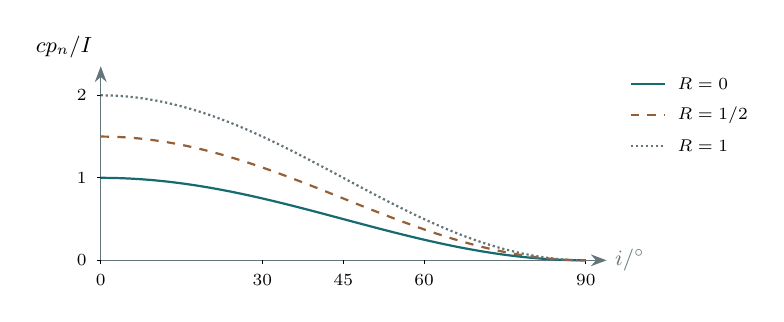
\begin{tikzpicture}[scale=.88,transform shape]
\draw[axis] (0,0.0)--(7.3,0.0) node[right] {$i/{}^\circ$};
\draw[axis] (0,0)--(0,2.8);
\node[above left] at (0,2.8) {$cp_n/I$};
\draw[thin] (0.000000,0.0)--(0.000000,-0.06);\node[below,font=\scriptsize] at (0.000000,-0.08) {$ 0 $};
\draw[thin] (2.333333,0.0)--(2.333333,-0.06);\node[below,font=\scriptsize] at (2.333333,-0.08) {$ 30 $};
\draw[thin] (3.500000,0.0)--(3.500000,-0.06);\node[below,font=\scriptsize] at (3.500000,-0.08) {$ 45 $};
\draw[thin] (4.666667,0.0)--(4.666667,-0.06);\node[below,font=\scriptsize] at (4.666667,-0.08) {$ 60 $};
\draw[thin] (7.000000,0.0)--(7.000000,-0.06);\node[below,font=\scriptsize] at (7.000000,-0.08) {$ 90 $};
\draw[thin] (0,0.000000)--(-.06,0.000000);\node[left,font=\scriptsize] at (-.08,0.000000) {$ 0 $};
\draw[thin] (0,1.190476)--(-.06,1.190476);\node[left,font=\scriptsize] at (-.08,1.190476) {$ 1 $};
\draw[thin] (0,2.380952)--(-.06,2.380952);\node[left,font=\scriptsize] at (-.08,2.380952) {$ 2 $};
\draw[thick,color=accent] plot coordinates {(0.0000000,1.1904762) (0.0291667,1.1904252) (0.0583333,1.1902722) (0.0875000,1.1900173) (0.1166667,1.1896604) (0.1458333,1.1892017) (0.1750000,1.1886413) (0.2041667,1.1879791) (0.2333333,1.1872154) (0.2625000,1.1863503) (0.2916667,1.1853838) (0.3208333,1.1843163) (0.3500000,1.1831478) (0.3791667,1.1818786) (0.4083333,1.1805089) (0.4375000,1.1790389) (0.4666667,1.1774688) (0.4958333,1.1757990) (0.5250000,1.1740297) (0.5541667,1.1721613) (0.5833333,1.1701939) (0.6125000,1.1681281) (0.6416667,1.1659641) (0.6708333,1.1637023) (0.7000000,1.1613432) (0.7291667,1.1588870) (0.7583333,1.1563342) (0.7875000,1.1536853) (0.8166667,1.1509407) (0.8458333,1.1481009) (0.8750000,1.1451664) (0.9041667,1.1421376) (0.9333333,1.1390152) (0.9625000,1.1357995) (0.9916667,1.1324912) (1.0208333,1.1290909) (1.0500000,1.1255991) (1.0791667,1.1220165) (1.1083333,1.1183435) (1.1375000,1.1145810) (1.1666667,1.1107294) (1.1958333,1.1067895) (1.2250000,1.1027620) (1.2541667,1.0986475) (1.2833333,1.0944468) (1.3125000,1.0901605) (1.3416667,1.0857894) (1.3708333,1.0813343) (1.4000000,1.0767958) (1.4291667,1.0721749) (1.4583333,1.0674722) (1.4875000,1.0626886) (1.5166667,1.0578250) (1.5458333,1.0528820) (1.5750000,1.0478607) (1.6041667,1.0427618) (1.6333333,1.0375862) (1.6625000,1.0323348) (1.6916667,1.0270086) (1.7208333,1.0216083) (1.7500000,1.0161350) (1.7791667,1.0105896) (1.8083333,1.0049730) (1.8375000,0.9992862) (1.8666667,0.9935301) (1.8958333,0.9877058) (1.9250000,0.9818143) (1.9541667,0.9758565) (1.9833333,0.9698336) (2.0125000,0.9637464) (2.0416667,0.9575961) (2.0708333,0.9513837) (2.1000000,0.9451103) (2.1291667,0.9387769) (2.1583333,0.9323847) (2.1875000,0.9259347) (2.2166667,0.9194280) (2.2458333,0.9128658) (2.2750000,0.9062491) (2.3041667,0.8995792) (2.3333333,0.8928571) (2.3625000,0.8860841) (2.3916667,0.8792612) (2.4208333,0.8723896) (2.4500000,0.8654705) (2.4791667,0.8585052) (2.5083333,0.8514947) (2.5375000,0.8444403) (2.5666667,0.8373432) (2.5958333,0.8302047) (2.6250000,0.8230259) (2.6541667,0.8158080) (2.6833333,0.8085524) (2.7125000,0.8012602) (2.7416667,0.7939327) (2.7708333,0.7865711) (2.8000000,0.7791768) (2.8291667,0.7717509) (2.8583333,0.7642948) (2.8875000,0.7568098) (2.9166667,0.7492971) (2.9458333,0.7417579) (2.9750000,0.7341937) (3.0041667,0.7266056) (3.0333333,0.7189951) (3.0625000,0.7113633) (3.0916667,0.7037116) (3.1208333,0.6960414) (3.1500000,0.6883538) (3.1791667,0.6806504) (3.2083333,0.6729323) (3.2375000,0.6652008) (3.2666667,0.6574574) (3.2958333,0.6497033) (3.3250000,0.6419399) (3.3541667,0.6341685) (3.3833333,0.6263905) (3.4125000,0.6186070) (3.4416667,0.6108196) (3.4708333,0.6030295) (3.5000000,0.5952381) (3.5291667,0.5874467) (3.5583333,0.5796566) (3.5875000,0.5718692) (3.6166667,0.5640857) (3.6458333,0.5563077) (3.6750000,0.5485363) (3.7041667,0.5407728) (3.7333333,0.5330188) (3.7625000,0.5252754) (3.7916667,0.5175439) (3.8208333,0.5098258) (3.8500000,0.5021223) (3.8791667,0.4944348) (3.9083333,0.4867646) (3.9375000,0.4791129) (3.9666667,0.4714811) (3.9958333,0.4638706) (4.0250000,0.4562825) (4.0541667,0.4487183) (4.0833333,0.4411791) (4.1125000,0.4336664) (4.1416667,0.4261813) (4.1708333,0.4187253) (4.2000000,0.4112994) (4.2291667,0.4039051) (4.2583333,0.3965435) (4.2875000,0.3892160) (4.3166667,0.3819238) (4.3458333,0.3746682) (4.3750000,0.3674503) (4.4041667,0.3602715) (4.4333333,0.3531330) (4.4625000,0.3460359) (4.4916667,0.3389815) (4.5208333,0.3319710) (4.5500000,0.3250057) (4.5791667,0.3180866) (4.6083333,0.3112150) (4.6375000,0.3043921) (4.6666667,0.2976190) (4.6958333,0.2908970) (4.7250000,0.2842270) (4.7541667,0.2776104) (4.7833333,0.2710482) (4.8125000,0.2645415) (4.8416667,0.2580915) (4.8708333,0.2516993) (4.9000000,0.2453659) (4.9291667,0.2390925) (4.9583333,0.2328801) (4.9875000,0.2267298) (5.0166667,0.2206426) (5.0458333,0.2146196) (5.0750000,0.2086619) (5.1041667,0.2027703) (5.1333333,0.1969461) (5.1625000,0.1911900) (5.1916667,0.1855032) (5.2208333,0.1798866) (5.2500000,0.1743412) (5.2791667,0.1688679) (5.3083333,0.1634676) (5.3375000,0.1581414) (5.3666667,0.1528900) (5.3958333,0.1477144) (5.4250000,0.1426155) (5.4541667,0.1375941) (5.4833333,0.1326512) (5.5125000,0.1277875) (5.5416667,0.1230040) (5.5708333,0.1183013) (5.6000000,0.1136804) (5.6291667,0.1091419) (5.6583333,0.1046868) (5.6875000,0.1003157) (5.7166667,0.0960294) (5.7458333,0.0918287) (5.7750000,0.0877142) (5.8041667,0.0836867) (5.8333333,0.0797468) (5.8625000,0.0758952) (5.8916667,0.0721327) (5.9208333,0.0684597) (5.9500000,0.0648771) (5.9791667,0.0613853) (6.0083333,0.0579849) (6.0375000,0.0546767) (6.0666667,0.0514610) (6.0958333,0.0483386) (6.1250000,0.0453098) (6.1541667,0.0423753) (6.1833333,0.0395355) (6.2125000,0.0367909) (6.2416667,0.0341420) (6.2708333,0.0315892) (6.3000000,0.0291330) (6.3291667,0.0267738) (6.3583333,0.0245121) (6.3875000,0.0223481) (6.4166667,0.0202822) (6.4458333,0.0183149) (6.4750000,0.0164465) (6.5041667,0.0146772) (6.5333333,0.0130074) (6.5625000,0.0114373) (6.5916667,0.0099673) (6.6208333,0.0085976) (6.6500000,0.0073284) (6.6791667,0.0061599) (6.7083333,0.0050923) (6.7375000,0.0041259) (6.7666667,0.0032608) (6.7958333,0.0024971) (6.8250000,0.0018349) (6.8541667,0.0012745) (6.8833333,0.0008158) (6.9125000,0.0004589) (6.9416667,0.0002040) (6.9708333,0.0000510) (7.0000000,0.0000000)};
\draw[thick,color=accent] (7.65,2.55)--(8.15,2.55);\node[right,font=\scriptsize] at (8.2,2.55) {$R=0$};
\draw[thick,dashed,color=warm] plot coordinates {(0.0000000,1.7857143) (0.0291667,1.7856378) (0.0583333,1.7854083) (0.0875000,1.7850259) (0.1166667,1.7844907) (0.1458333,1.7838026) (0.1750000,1.7829619) (0.2041667,1.7819687) (0.2333333,1.7808231) (0.2625000,1.7795254) (0.2916667,1.7780758) (0.3208333,1.7764745) (0.3500000,1.7747217) (0.3791667,1.7728179) (0.4083333,1.7707633) (0.4375000,1.7685583) (0.4666667,1.7662032) (0.4958333,1.7636985) (0.5250000,1.7610446) (0.5541667,1.7582419) (0.5833333,1.7552909) (0.6125000,1.7521922) (0.6416667,1.7489462) (0.6708333,1.7455535) (0.7000000,1.7420147) (0.7291667,1.7383305) (0.7583333,1.7345013) (0.7875000,1.7305280) (0.8166667,1.7264111) (0.8458333,1.7221514) (0.8750000,1.7177496) (0.9041667,1.7132064) (0.9333333,1.7085227) (0.9625000,1.7036993) (0.9916667,1.6987369) (1.0208333,1.6936364) (1.0500000,1.6883987) (1.0791667,1.6830247) (1.1083333,1.6775153) (1.1375000,1.6718714) (1.1666667,1.6660941) (1.1958333,1.6601843) (1.2250000,1.6541430) (1.2541667,1.6479713) (1.2833333,1.6416701) (1.3125000,1.6352407) (1.3416667,1.6286841) (1.3708333,1.6220014) (1.4000000,1.6151937) (1.4291667,1.6082623) (1.4583333,1.6012083) (1.4875000,1.5940330) (1.5166667,1.5867375) (1.5458333,1.5793231) (1.5750000,1.5717910) (1.6041667,1.5641427) (1.6333333,1.5563793) (1.6625000,1.5485022) (1.6916667,1.5405128) (1.7208333,1.5324124) (1.7500000,1.5242025) (1.7791667,1.5158843) (1.8083333,1.5074594) (1.8375000,1.4989292) (1.8666667,1.4902952) (1.8958333,1.4815588) (1.9250000,1.4727215) (1.9541667,1.4637848) (1.9833333,1.4547503) (2.0125000,1.4456196) (2.0416667,1.4363941) (2.0708333,1.4270755) (2.1000000,1.4176654) (2.1291667,1.4081653) (2.1583333,1.3985770) (2.1875000,1.3889020) (2.2166667,1.3791420) (2.2458333,1.3692987) (2.2750000,1.3593737) (2.3041667,1.3493688) (2.3333333,1.3392857) (2.3625000,1.3291261) (2.3916667,1.3188918) (2.4208333,1.3085844) (2.4500000,1.2982058) (2.4791667,1.2877578) (2.5083333,1.2772421) (2.5375000,1.2666605) (2.5666667,1.2560149) (2.5958333,1.2453070) (2.6250000,1.2345388) (2.6541667,1.2237120) (2.6833333,1.2128285) (2.7125000,1.2018902) (2.7416667,1.1908990) (2.7708333,1.1798567) (2.8000000,1.1687652) (2.8291667,1.1576264) (2.8583333,1.1464423) (2.8875000,1.1352147) (2.9166667,1.1239456) (2.9458333,1.1126369) (2.9750000,1.1012905) (3.0041667,1.0899084) (3.0333333,1.0784926) (3.0625000,1.0670449) (3.0916667,1.0555674) (3.1208333,1.0440621) (3.1500000,1.0325308) (3.1791667,1.0209756) (3.2083333,1.0093984) (3.2375000,0.9978012) (3.2666667,0.9861861) (3.2958333,0.9745550) (3.3250000,0.9629099) (3.3541667,0.9512528) (3.3833333,0.9395857) (3.4125000,0.9279105) (3.4416667,0.9162294) (3.4708333,0.9045443) (3.5000000,0.8928571) (3.5291667,0.8811700) (3.5583333,0.8694849) (3.5875000,0.8578037) (3.6166667,0.8461286) (3.6458333,0.8344615) (3.6750000,0.8228044) (3.7041667,0.8111593) (3.7333333,0.7995282) (3.7625000,0.7879130) (3.7916667,0.7763159) (3.8208333,0.7647387) (3.8500000,0.7531835) (3.8791667,0.7416522) (3.9083333,0.7301469) (3.9375000,0.7186694) (3.9666667,0.7072217) (3.9958333,0.6958059) (4.0250000,0.6844238) (4.0541667,0.6730774) (4.0833333,0.6617687) (4.1125000,0.6504996) (4.1416667,0.6392720) (4.1708333,0.6280879) (4.2000000,0.6169491) (4.2291667,0.6058576) (4.2583333,0.5948153) (4.2875000,0.5838241) (4.3166667,0.5728858) (4.3458333,0.5620023) (4.3750000,0.5511755) (4.4041667,0.5404073) (4.4333333,0.5296994) (4.4625000,0.5190538) (4.4916667,0.5084722) (4.5208333,0.4979565) (4.5500000,0.4875085) (4.5791667,0.4771299) (4.6083333,0.4668225) (4.6375000,0.4565882) (4.6666667,0.4464286) (4.6958333,0.4363455) (4.7250000,0.4263406) (4.7541667,0.4164156) (4.7833333,0.4065723) (4.8125000,0.3968123) (4.8416667,0.3871373) (4.8708333,0.3775489) (4.9000000,0.3680489) (4.9291667,0.3586387) (4.9583333,0.3493202) (4.9875000,0.3400947) (5.0166667,0.3309639) (5.0458333,0.3219295) (5.0750000,0.3129928) (5.1041667,0.3041555) (5.1333333,0.2954191) (5.1625000,0.2867850) (5.1916667,0.2782548) (5.2208333,0.2698299) (5.2500000,0.2615118) (5.2791667,0.2533018) (5.3083333,0.2452015) (5.3375000,0.2372120) (5.3666667,0.2293350) (5.3958333,0.2215716) (5.4250000,0.2139232) (5.4541667,0.2063912) (5.4833333,0.1989768) (5.5125000,0.1916813) (5.5416667,0.1845059) (5.5708333,0.1774520) (5.6000000,0.1705205) (5.6291667,0.1637129) (5.6583333,0.1570302) (5.6875000,0.1504736) (5.7166667,0.1440441) (5.7458333,0.1377430) (5.7750000,0.1315713) (5.8041667,0.1255300) (5.8333333,0.1196202) (5.8625000,0.1138429) (5.8916667,0.1081990) (5.9208333,0.1026896) (5.9500000,0.0973156) (5.9791667,0.0920779) (6.0083333,0.0869774) (6.0375000,0.0820150) (6.0666667,0.0771916) (6.0958333,0.0725078) (6.1250000,0.0679647) (6.1541667,0.0635629) (6.1833333,0.0593032) (6.2125000,0.0551863) (6.2416667,0.0512130) (6.2708333,0.0473838) (6.3000000,0.0436995) (6.3291667,0.0401608) (6.3583333,0.0367681) (6.3875000,0.0335221) (6.4166667,0.0304234) (6.4458333,0.0274724) (6.4750000,0.0246697) (6.5041667,0.0220158) (6.5333333,0.0195111) (6.5625000,0.0171560) (6.5916667,0.0149510) (6.6208333,0.0128964) (6.6500000,0.0109926) (6.6791667,0.0092398) (6.7083333,0.0076385) (6.7375000,0.0061889) (6.7666667,0.0048912) (6.7958333,0.0037456) (6.8250000,0.0027524) (6.8541667,0.0019117) (6.8833333,0.0012236) (6.9125000,0.0006884) (6.9416667,0.0003060) (6.9708333,0.0000765) (7.0000000,0.0000000)};
\draw[thick,dashed,color=warm] (7.65,2.0999999999999996)--(8.15,2.0999999999999996);\node[right,font=\scriptsize] at (8.2,2.0999999999999996) {$R=1/2$};
\draw[densely dotted,thick,color=muted] plot coordinates {(0.0000000,2.3809524) (0.0291667,2.3808504) (0.0583333,2.3805444) (0.0875000,2.3800346) (0.1166667,2.3793209) (0.1458333,2.3784035) (0.1750000,2.3772825) (0.2041667,2.3759582) (0.2333333,2.3744308) (0.2625000,2.3727005) (0.2916667,2.3707677) (0.3208333,2.3686326) (0.3500000,2.3662956) (0.3791667,2.3637572) (0.4083333,2.3610177) (0.4375000,2.3580777) (0.4666667,2.3549376) (0.4958333,2.3515980) (0.5250000,2.3480594) (0.5541667,2.3443225) (0.5833333,2.3403879) (0.6125000,2.3362562) (0.6416667,2.3319283) (0.6708333,2.3274047) (0.7000000,2.3226863) (0.7291667,2.3177740) (0.7583333,2.3126684) (0.7875000,2.3073706) (0.8166667,2.3018815) (0.8458333,2.2962018) (0.8750000,2.2903328) (0.9041667,2.2842753) (0.9333333,2.2780303) (0.9625000,2.2715990) (0.9916667,2.2649825) (1.0208333,2.2581818) (1.0500000,2.2511982) (1.0791667,2.2440329) (1.1083333,2.2366870) (1.1375000,2.2291619) (1.1666667,2.2214588) (1.1958333,2.2135791) (1.2250000,2.2055240) (1.2541667,2.1972950) (1.2833333,2.1888935) (1.3125000,2.1803210) (1.3416667,2.1715788) (1.3708333,2.1626685) (1.4000000,2.1535917) (1.4291667,2.1443498) (1.4583333,2.1349445) (1.4875000,2.1253773) (1.5166667,2.1156500) (1.5458333,2.1057641) (1.5750000,2.0957214) (1.6041667,2.0855236) (1.6333333,2.0751724) (1.6625000,2.0646697) (1.6916667,2.0540171) (1.7208333,2.0432166) (1.7500000,2.0322700) (1.7791667,2.0211791) (1.8083333,2.0099459) (1.8375000,1.9985723) (1.8666667,1.9870602) (1.8958333,1.9754117) (1.9250000,1.9636286) (1.9541667,1.9517131) (1.9833333,1.9396671) (2.0125000,1.9274928) (2.0416667,1.9151922) (2.0708333,1.9027674) (2.1000000,1.8902205) (2.1291667,1.8775538) (2.1583333,1.8647693) (2.1875000,1.8518693) (2.2166667,1.8388560) (2.2458333,1.8257316) (2.2750000,1.8124983) (2.3041667,1.7991584) (2.3333333,1.7857143) (2.3625000,1.7721681) (2.3916667,1.7585223) (2.4208333,1.7447792) (2.4500000,1.7309411) (2.4791667,1.7170103) (2.5083333,1.7029894) (2.5375000,1.6888806) (2.5666667,1.6746865) (2.5958333,1.6604094) (2.6250000,1.6460517) (2.6541667,1.6316160) (2.6833333,1.6171047) (2.7125000,1.6025203) (2.7416667,1.5878653) (2.7708333,1.5731422) (2.8000000,1.5583536) (2.8291667,1.5435019) (2.8583333,1.5285897) (2.8875000,1.5136196) (2.9166667,1.4985941) (2.9458333,1.4835158) (2.9750000,1.4683873) (3.0041667,1.4532112) (3.0333333,1.4379901) (3.0625000,1.4227266) (3.0916667,1.4074232) (3.1208333,1.3920827) (3.1500000,1.3767077) (3.1791667,1.3613007) (3.2083333,1.3458645) (3.2375000,1.3304017) (3.2666667,1.3149148) (3.2958333,1.2994067) (3.3250000,1.2838799) (3.3541667,1.2683371) (3.3833333,1.2527809) (3.4125000,1.2372141) (3.4416667,1.2216392) (3.4708333,1.2060590) (3.5000000,1.1904762) (3.5291667,1.1748933) (3.5583333,1.1593132) (3.5875000,1.1437383) (3.6166667,1.1281715) (3.6458333,1.1126153) (3.6750000,1.0970725) (3.7041667,1.0815457) (3.7333333,1.0660375) (3.7625000,1.0505507) (3.7916667,1.0350879) (3.8208333,1.0196516) (3.8500000,1.0042447) (3.8791667,0.9888696) (3.9083333,0.9735291) (3.9375000,0.9582258) (3.9666667,0.9429623) (3.9958333,0.9277411) (4.0250000,0.9125650) (4.0541667,0.8974366) (4.0833333,0.8823583) (4.1125000,0.8673328) (4.1416667,0.8523627) (4.1708333,0.8374505) (4.2000000,0.8225988) (4.2291667,0.8078102) (4.2583333,0.7930871) (4.2875000,0.7784321) (4.3166667,0.7638477) (4.3458333,0.7493364) (4.3750000,0.7349007) (4.4041667,0.7205430) (4.4333333,0.7062659) (4.4625000,0.6920717) (4.4916667,0.6779630) (4.5208333,0.6639420) (4.5500000,0.6500113) (4.5791667,0.6361732) (4.6083333,0.6224300) (4.6375000,0.6087842) (4.6666667,0.5952381) (4.6958333,0.5817939) (4.7250000,0.5684541) (4.7541667,0.5552208) (4.7833333,0.5420964) (4.8125000,0.5290831) (4.8416667,0.5161831) (4.8708333,0.5033986) (4.9000000,0.4907318) (4.9291667,0.4781850) (4.9583333,0.4657602) (4.9875000,0.4534596) (5.0166667,0.4412852) (5.0458333,0.4292393) (5.0750000,0.4173238) (5.1041667,0.4055407) (5.1333333,0.3938921) (5.1625000,0.3823801) (5.1916667,0.3710065) (5.2208333,0.3597733) (5.2500000,0.3486824) (5.2791667,0.3377358) (5.3083333,0.3269353) (5.3375000,0.3162827) (5.3666667,0.3057800) (5.3958333,0.2954288) (5.4250000,0.2852310) (5.4541667,0.2751883) (5.4833333,0.2653024) (5.5125000,0.2555751) (5.5416667,0.2460079) (5.5708333,0.2366026) (5.6000000,0.2273607) (5.6291667,0.2182839) (5.6583333,0.2093736) (5.6875000,0.2006314) (5.7166667,0.1920588) (5.7458333,0.1836574) (5.7750000,0.1754284) (5.8041667,0.1673733) (5.8333333,0.1594936) (5.8625000,0.1517905) (5.8916667,0.1442653) (5.9208333,0.1369195) (5.9500000,0.1297541) (5.9791667,0.1227705) (6.0083333,0.1159699) (6.0375000,0.1093534) (6.0666667,0.1029221) (6.0958333,0.0966771) (6.1250000,0.0906196) (6.1541667,0.0847505) (6.1833333,0.0790709) (6.2125000,0.0735817) (6.2416667,0.0682839) (6.2708333,0.0631784) (6.3000000,0.0582661) (6.3291667,0.0535477) (6.3583333,0.0490241) (6.3875000,0.0446961) (6.4166667,0.0405645) (6.4458333,0.0366299) (6.4750000,0.0328930) (6.5041667,0.0293544) (6.5333333,0.0260148) (6.5625000,0.0228747) (6.5916667,0.0199346) (6.6208333,0.0171952) (6.6500000,0.0146567) (6.6791667,0.0123198) (6.7083333,0.0101847) (6.7375000,0.0082518) (6.7666667,0.0065216) (6.7958333,0.0049941) (6.8250000,0.0036698) (6.8541667,0.0025489) (6.8833333,0.0016315) (6.9125000,0.0009178) (6.9416667,0.0004079) (6.9708333,0.0001020) (7.0000000,0.0000000)};
\draw[densely dotted,thick,color=muted] (7.65,1.65)--(8.15,1.65);\node[right,font=\scriptsize] at (8.2,1.65) {$R=1$};
\end{tikzpicture}
\figcaption{解图近1.1C\quad 镜面反射增强给表面的法向动量}
\end{minipage}\end{center}
\begin{center}\begin{minipage}{.98\linewidth}\centering
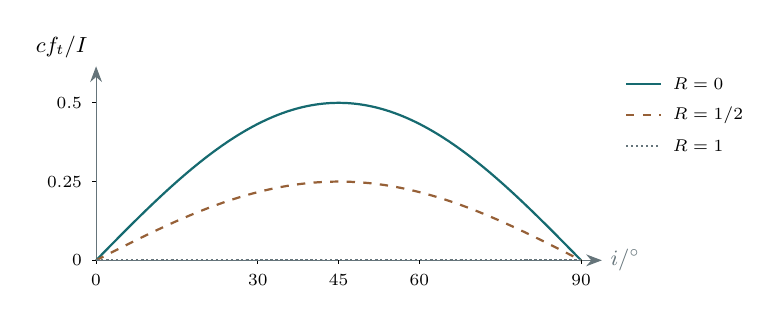
\begin{tikzpicture}[scale=.88,transform shape]
\draw[axis] (0,0.0)--(7.3,0.0) node[right] {$i/{}^\circ$};
\draw[axis] (0,0)--(0,2.8);
\node[above left] at (0,2.8) {$cf_t/I$};
\draw[thin] (0.000000,0.0)--(0.000000,-0.06);\node[below,font=\scriptsize] at (0.000000,-0.08) {$ 0 $};
\draw[thin] (2.333333,0.0)--(2.333333,-0.06);\node[below,font=\scriptsize] at (2.333333,-0.08) {$ 30 $};
\draw[thin] (3.500000,0.0)--(3.500000,-0.06);\node[below,font=\scriptsize] at (3.500000,-0.08) {$ 45 $};
\draw[thin] (4.666667,0.0)--(4.666667,-0.06);\node[below,font=\scriptsize] at (4.666667,-0.08) {$ 60 $};
\draw[thin] (7.000000,0.0)--(7.000000,-0.06);\node[below,font=\scriptsize] at (7.000000,-0.08) {$ 90 $};
\draw[thin] (0,0.000000)--(-.06,0.000000);\node[left,font=\scriptsize] at (-.08,0.000000) {$ 0 $};
\draw[thin] (0,1.136364)--(-.06,1.136364);\node[left,font=\scriptsize] at (-.08,1.136364) {$ 0.25 $};
\draw[thin] (0,2.272727)--(-.06,2.272727);\node[left,font=\scriptsize] at (-.08,2.272727) {$ 0.5 $};
\draw[thick,color=accent] plot coordinates {(0.0000000,0.0000000) (0.0291667,0.0297491) (0.0583333,0.0594931) (0.0875000,0.0892269) (0.1166667,0.1189454) (0.1458333,0.1486435) (0.1750000,0.1783161) (0.2041667,0.2079582) (0.2333333,0.2375647) (0.2625000,0.2671304) (0.2916667,0.2966504) (0.3208333,0.3261196) (0.3500000,0.3555329) (0.3791667,0.3848852) (0.4083333,0.4141716) (0.4375000,0.4433871) (0.4666667,0.4725266) (0.4958333,0.5015851) (0.5250000,0.5305576) (0.5541667,0.5594393) (0.5833333,0.5882251) (0.6125000,0.6169101) (0.6416667,0.6454894) (0.6708333,0.6739581) (0.7000000,0.7023114) (0.7291667,0.7305442) (0.7583333,0.7586520) (0.7875000,0.7866297) (0.8166667,0.8144726) (0.8458333,0.8421760) (0.8750000,0.8697351) (0.9041667,0.8971451) (0.9333333,0.9244015) (0.9625000,0.9514994) (0.9916667,0.9784343) (1.0208333,1.0052016) (1.0500000,1.0317966) (1.0791667,1.0582148) (1.1083333,1.0844517) (1.1375000,1.1105028) (1.1666667,1.1363636) (1.1958333,1.1620297) (1.2250000,1.1874967) (1.2541667,1.2127603) (1.2833333,1.2378160) (1.3125000,1.2626596) (1.3416667,1.2872869) (1.3708333,1.3116936) (1.4000000,1.3358756) (1.4291667,1.3598286) (1.4583333,1.3835487) (1.4875000,1.4070317) (1.5166667,1.4302736) (1.5458333,1.4532705) (1.5750000,1.4760183) (1.6041667,1.4985132) (1.6333333,1.5207514) (1.6625000,1.5427290) (1.6916667,1.5644422) (1.7208333,1.5858874) (1.7500000,1.6070609) (1.7791667,1.6279590) (1.8083333,1.6485781) (1.8375000,1.6689148) (1.8666667,1.6889655) (1.8958333,1.7087268) (1.9250000,1.7281954) (1.9541667,1.7473678) (1.9833333,1.7662408) (2.0125000,1.7848112) (2.0416667,1.8030758) (2.0708333,1.8210314) (2.1000000,1.8386750) (2.1291667,1.8560035) (2.1583333,1.8730141) (2.1875000,1.8897037) (2.2166667,1.9060695) (2.2458333,1.9221087) (2.2750000,1.9378186) (2.3041667,1.9531964) (2.3333333,1.9682396) (2.3625000,1.9829455) (2.3916667,1.9973116) (2.4208333,2.0113355) (2.4500000,2.0250148) (2.4791667,2.0383471) (2.5083333,2.0513302) (2.5375000,2.0639618) (2.5666667,2.0762397) (2.5958333,2.0881618) (2.6250000,2.0997262) (2.6541667,2.1109308) (2.6833333,2.1217737) (2.7125000,2.1322530) (2.7416667,2.1423670) (2.7708333,2.1521139) (2.8000000,2.1614921) (2.8291667,2.1704999) (2.8583333,2.1791358) (2.8875000,2.1873983) (2.9166667,2.1952860) (2.9458333,2.2027975) (2.9750000,2.2099316) (3.0041667,2.2166871) (3.0333333,2.2230627) (3.0625000,2.2290575) (3.0916667,2.2346702) (3.1208333,2.2399001) (3.1500000,2.2447462) (3.1791667,2.2492077) (3.2083333,2.2532838) (3.2375000,2.2569738) (3.2666667,2.2602770) (3.2958333,2.2631930) (3.3250000,2.2657212) (3.3541667,2.2678612) (3.3833333,2.2696126) (3.4125000,2.2709751) (3.4416667,2.2719485) (3.4708333,2.2725326) (3.5000000,2.2727273) (3.5291667,2.2725326) (3.5583333,2.2719485) (3.5875000,2.2709751) (3.6166667,2.2696126) (3.6458333,2.2678612) (3.6750000,2.2657212) (3.7041667,2.2631930) (3.7333333,2.2602770) (3.7625000,2.2569738) (3.7916667,2.2532838) (3.8208333,2.2492077) (3.8500000,2.2447462) (3.8791667,2.2399001) (3.9083333,2.2346702) (3.9375000,2.2290575) (3.9666667,2.2230627) (3.9958333,2.2166871) (4.0250000,2.2099316) (4.0541667,2.2027975) (4.0833333,2.1952860) (4.1125000,2.1873983) (4.1416667,2.1791358) (4.1708333,2.1704999) (4.2000000,2.1614921) (4.2291667,2.1521139) (4.2583333,2.1423670) (4.2875000,2.1322530) (4.3166667,2.1217737) (4.3458333,2.1109308) (4.3750000,2.0997262) (4.4041667,2.0881618) (4.4333333,2.0762397) (4.4625000,2.0639618) (4.4916667,2.0513302) (4.5208333,2.0383471) (4.5500000,2.0250148) (4.5791667,2.0113355) (4.6083333,1.9973116) (4.6375000,1.9829455) (4.6666667,1.9682396) (4.6958333,1.9531964) (4.7250000,1.9378186) (4.7541667,1.9221087) (4.7833333,1.9060695) (4.8125000,1.8897037) (4.8416667,1.8730141) (4.8708333,1.8560035) (4.9000000,1.8386750) (4.9291667,1.8210314) (4.9583333,1.8030758) (4.9875000,1.7848112) (5.0166667,1.7662408) (5.0458333,1.7473678) (5.0750000,1.7281954) (5.1041667,1.7087268) (5.1333333,1.6889655) (5.1625000,1.6689148) (5.1916667,1.6485781) (5.2208333,1.6279590) (5.2500000,1.6070609) (5.2791667,1.5858874) (5.3083333,1.5644422) (5.3375000,1.5427290) (5.3666667,1.5207514) (5.3958333,1.4985132) (5.4250000,1.4760183) (5.4541667,1.4532705) (5.4833333,1.4302736) (5.5125000,1.4070317) (5.5416667,1.3835487) (5.5708333,1.3598286) (5.6000000,1.3358756) (5.6291667,1.3116936) (5.6583333,1.2872869) (5.6875000,1.2626596) (5.7166667,1.2378160) (5.7458333,1.2127603) (5.7750000,1.1874967) (5.8041667,1.1620297) (5.8333333,1.1363636) (5.8625000,1.1105028) (5.8916667,1.0844517) (5.9208333,1.0582148) (5.9500000,1.0317966) (5.9791667,1.0052016) (6.0083333,0.9784343) (6.0375000,0.9514994) (6.0666667,0.9244015) (6.0958333,0.8971451) (6.1250000,0.8697351) (6.1541667,0.8421760) (6.1833333,0.8144726) (6.2125000,0.7866297) (6.2416667,0.7586520) (6.2708333,0.7305442) (6.3000000,0.7023114) (6.3291667,0.6739581) (6.3583333,0.6454894) (6.3875000,0.6169101) (6.4166667,0.5882251) (6.4458333,0.5594393) (6.4750000,0.5305576) (6.5041667,0.5015851) (6.5333333,0.4725266) (6.5625000,0.4433871) (6.5916667,0.4141716) (6.6208333,0.3848852) (6.6500000,0.3555329) (6.6791667,0.3261196) (6.7083333,0.2966504) (6.7375000,0.2671304) (6.7666667,0.2375647) (6.7958333,0.2079582) (6.8250000,0.1783161) (6.8541667,0.1486435) (6.8833333,0.1189454) (6.9125000,0.0892269) (6.9416667,0.0594931) (6.9708333,0.0297491) (7.0000000,0.0000000)};
\draw[thick,color=accent] (7.65,2.55)--(8.15,2.55);\node[right,font=\scriptsize] at (8.2,2.55) {$R=0$};
\draw[thick,dashed,color=warm] plot coordinates {(0.0000000,0.0000000) (0.0291667,0.0148745) (0.0583333,0.0297465) (0.0875000,0.0446134) (0.1166667,0.0594727) (0.1458333,0.0743217) (0.1750000,0.0891581) (0.2041667,0.1039791) (0.2333333,0.1187823) (0.2625000,0.1335652) (0.2916667,0.1483252) (0.3208333,0.1630598) (0.3500000,0.1777664) (0.3791667,0.1924426) (0.4083333,0.2070858) (0.4375000,0.2216935) (0.4666667,0.2362633) (0.4958333,0.2507925) (0.5250000,0.2652788) (0.5541667,0.2797197) (0.5833333,0.2941126) (0.6125000,0.3084551) (0.6416667,0.3227447) (0.6708333,0.3369791) (0.7000000,0.3511557) (0.7291667,0.3652721) (0.7583333,0.3793260) (0.7875000,0.3933148) (0.8166667,0.4072363) (0.8458333,0.4210880) (0.8750000,0.4348675) (0.9041667,0.4485726) (0.9333333,0.4622007) (0.9625000,0.4757497) (0.9916667,0.4892172) (1.0208333,0.5026008) (1.0500000,0.5158983) (1.0791667,0.5291074) (1.1083333,0.5422259) (1.1375000,0.5552514) (1.1666667,0.5681818) (1.1958333,0.5810149) (1.2250000,0.5937484) (1.2541667,0.6063801) (1.2833333,0.6189080) (1.3125000,0.6313298) (1.3416667,0.6436435) (1.3708333,0.6558468) (1.4000000,0.6679378) (1.4291667,0.6799143) (1.4583333,0.6917744) (1.4875000,0.7035159) (1.5166667,0.7151368) (1.5458333,0.7266352) (1.5750000,0.7380091) (1.6041667,0.7492566) (1.6333333,0.7603757) (1.6625000,0.7713645) (1.6916667,0.7822211) (1.7208333,0.7929437) (1.7500000,0.8035304) (1.7791667,0.8139795) (1.8083333,0.8242891) (1.8375000,0.8344574) (1.8666667,0.8444828) (1.8958333,0.8543634) (1.9250000,0.8640977) (1.9541667,0.8736839) (1.9833333,0.8831204) (2.0125000,0.8924056) (2.0416667,0.9015379) (2.0708333,0.9105157) (2.1000000,0.9193375) (2.1291667,0.9280018) (2.1583333,0.9365070) (2.1875000,0.9448518) (2.2166667,0.9530347) (2.2458333,0.9610543) (2.2750000,0.9689093) (2.3041667,0.9765982) (2.3333333,0.9841198) (2.3625000,0.9914727) (2.3916667,0.9986558) (2.4208333,1.0056678) (2.4500000,1.0125074) (2.4791667,1.0191736) (2.5083333,1.0256651) (2.5375000,1.0319809) (2.5666667,1.0381198) (2.5958333,1.0440809) (2.6250000,1.0498631) (2.6541667,1.0554654) (2.6833333,1.0608868) (2.7125000,1.0661265) (2.7416667,1.0711835) (2.7708333,1.0760570) (2.8000000,1.0807460) (2.8291667,1.0852499) (2.8583333,1.0895679) (2.8875000,1.0936991) (2.9166667,1.0976430) (2.9458333,1.1013988) (2.9750000,1.1049658) (3.0041667,1.1083435) (3.0333333,1.1115314) (3.0625000,1.1145287) (3.0916667,1.1173351) (3.1208333,1.1199501) (3.1500000,1.1223731) (3.1791667,1.1246038) (3.2083333,1.1266419) (3.2375000,1.1284869) (3.2666667,1.1301385) (3.2958333,1.1315965) (3.3250000,1.1328606) (3.3541667,1.1339306) (3.3833333,1.1348063) (3.4125000,1.1354875) (3.4416667,1.1359742) (3.4708333,1.1362663) (3.5000000,1.1363636) (3.5291667,1.1362663) (3.5583333,1.1359742) (3.5875000,1.1354875) (3.6166667,1.1348063) (3.6458333,1.1339306) (3.6750000,1.1328606) (3.7041667,1.1315965) (3.7333333,1.1301385) (3.7625000,1.1284869) (3.7916667,1.1266419) (3.8208333,1.1246038) (3.8500000,1.1223731) (3.8791667,1.1199501) (3.9083333,1.1173351) (3.9375000,1.1145287) (3.9666667,1.1115314) (3.9958333,1.1083435) (4.0250000,1.1049658) (4.0541667,1.1013988) (4.0833333,1.0976430) (4.1125000,1.0936991) (4.1416667,1.0895679) (4.1708333,1.0852499) (4.2000000,1.0807460) (4.2291667,1.0760570) (4.2583333,1.0711835) (4.2875000,1.0661265) (4.3166667,1.0608868) (4.3458333,1.0554654) (4.3750000,1.0498631) (4.4041667,1.0440809) (4.4333333,1.0381198) (4.4625000,1.0319809) (4.4916667,1.0256651) (4.5208333,1.0191736) (4.5500000,1.0125074) (4.5791667,1.0056678) (4.6083333,0.9986558) (4.6375000,0.9914727) (4.6666667,0.9841198) (4.6958333,0.9765982) (4.7250000,0.9689093) (4.7541667,0.9610543) (4.7833333,0.9530347) (4.8125000,0.9448518) (4.8416667,0.9365070) (4.8708333,0.9280018) (4.9000000,0.9193375) (4.9291667,0.9105157) (4.9583333,0.9015379) (4.9875000,0.8924056) (5.0166667,0.8831204) (5.0458333,0.8736839) (5.0750000,0.8640977) (5.1041667,0.8543634) (5.1333333,0.8444828) (5.1625000,0.8344574) (5.1916667,0.8242891) (5.2208333,0.8139795) (5.2500000,0.8035304) (5.2791667,0.7929437) (5.3083333,0.7822211) (5.3375000,0.7713645) (5.3666667,0.7603757) (5.3958333,0.7492566) (5.4250000,0.7380091) (5.4541667,0.7266352) (5.4833333,0.7151368) (5.5125000,0.7035159) (5.5416667,0.6917744) (5.5708333,0.6799143) (5.6000000,0.6679378) (5.6291667,0.6558468) (5.6583333,0.6436435) (5.6875000,0.6313298) (5.7166667,0.6189080) (5.7458333,0.6063801) (5.7750000,0.5937484) (5.8041667,0.5810149) (5.8333333,0.5681818) (5.8625000,0.5552514) (5.8916667,0.5422259) (5.9208333,0.5291074) (5.9500000,0.5158983) (5.9791667,0.5026008) (6.0083333,0.4892172) (6.0375000,0.4757497) (6.0666667,0.4622007) (6.0958333,0.4485726) (6.1250000,0.4348675) (6.1541667,0.4210880) (6.1833333,0.4072363) (6.2125000,0.3933148) (6.2416667,0.3793260) (6.2708333,0.3652721) (6.3000000,0.3511557) (6.3291667,0.3369791) (6.3583333,0.3227447) (6.3875000,0.3084551) (6.4166667,0.2941126) (6.4458333,0.2797197) (6.4750000,0.2652788) (6.5041667,0.2507925) (6.5333333,0.2362633) (6.5625000,0.2216935) (6.5916667,0.2070858) (6.6208333,0.1924426) (6.6500000,0.1777664) (6.6791667,0.1630598) (6.7083333,0.1483252) (6.7375000,0.1335652) (6.7666667,0.1187823) (6.7958333,0.1039791) (6.8250000,0.0891581) (6.8541667,0.0743217) (6.8833333,0.0594727) (6.9125000,0.0446134) (6.9416667,0.0297465) (6.9708333,0.0148745) (7.0000000,0.0000000)};
\draw[thick,dashed,color=warm] (7.65,2.0999999999999996)--(8.15,2.0999999999999996);\node[right,font=\scriptsize] at (8.2,2.0999999999999996) {$R=1/2$};
\draw[densely dotted,thick,color=muted] plot coordinates {(0.0000000,0.0000000) (0.0291667,0.0000000) (0.0583333,0.0000000) (0.0875000,0.0000000) (0.1166667,0.0000000) (0.1458333,0.0000000) (0.1750000,0.0000000) (0.2041667,0.0000000) (0.2333333,0.0000000) (0.2625000,0.0000000) (0.2916667,0.0000000) (0.3208333,0.0000000) (0.3500000,0.0000000) (0.3791667,0.0000000) (0.4083333,0.0000000) (0.4375000,0.0000000) (0.4666667,0.0000000) (0.4958333,0.0000000) (0.5250000,0.0000000) (0.5541667,0.0000000) (0.5833333,0.0000000) (0.6125000,0.0000000) (0.6416667,0.0000000) (0.6708333,0.0000000) (0.7000000,0.0000000) (0.7291667,0.0000000) (0.7583333,0.0000000) (0.7875000,0.0000000) (0.8166667,0.0000000) (0.8458333,0.0000000) (0.8750000,0.0000000) (0.9041667,0.0000000) (0.9333333,0.0000000) (0.9625000,0.0000000) (0.9916667,0.0000000) (1.0208333,0.0000000) (1.0500000,0.0000000) (1.0791667,0.0000000) (1.1083333,0.0000000) (1.1375000,0.0000000) (1.1666667,0.0000000) (1.1958333,0.0000000) (1.2250000,0.0000000) (1.2541667,0.0000000) (1.2833333,0.0000000) (1.3125000,0.0000000) (1.3416667,0.0000000) (1.3708333,0.0000000) (1.4000000,0.0000000) (1.4291667,0.0000000) (1.4583333,0.0000000) (1.4875000,0.0000000) (1.5166667,0.0000000) (1.5458333,0.0000000) (1.5750000,0.0000000) (1.6041667,0.0000000) (1.6333333,0.0000000) (1.6625000,0.0000000) (1.6916667,0.0000000) (1.7208333,0.0000000) (1.7500000,0.0000000) (1.7791667,0.0000000) (1.8083333,0.0000000) (1.8375000,0.0000000) (1.8666667,0.0000000) (1.8958333,0.0000000) (1.9250000,0.0000000) (1.9541667,0.0000000) (1.9833333,0.0000000) (2.0125000,0.0000000) (2.0416667,0.0000000) (2.0708333,0.0000000) (2.1000000,0.0000000) (2.1291667,0.0000000) (2.1583333,0.0000000) (2.1875000,0.0000000) (2.2166667,0.0000000) (2.2458333,0.0000000) (2.2750000,0.0000000) (2.3041667,0.0000000) (2.3333333,0.0000000) (2.3625000,0.0000000) (2.3916667,0.0000000) (2.4208333,0.0000000) (2.4500000,0.0000000) (2.4791667,0.0000000) (2.5083333,0.0000000) (2.5375000,0.0000000) (2.5666667,0.0000000) (2.5958333,0.0000000) (2.6250000,0.0000000) (2.6541667,0.0000000) (2.6833333,0.0000000) (2.7125000,0.0000000) (2.7416667,0.0000000) (2.7708333,0.0000000) (2.8000000,0.0000000) (2.8291667,0.0000000) (2.8583333,0.0000000) (2.8875000,0.0000000) (2.9166667,0.0000000) (2.9458333,0.0000000) (2.9750000,0.0000000) (3.0041667,0.0000000) (3.0333333,0.0000000) (3.0625000,0.0000000) (3.0916667,0.0000000) (3.1208333,0.0000000) (3.1500000,0.0000000) (3.1791667,0.0000000) (3.2083333,0.0000000) (3.2375000,0.0000000) (3.2666667,0.0000000) (3.2958333,0.0000000) (3.3250000,0.0000000) (3.3541667,0.0000000) (3.3833333,0.0000000) (3.4125000,0.0000000) (3.4416667,0.0000000) (3.4708333,0.0000000) (3.5000000,0.0000000) (3.5291667,0.0000000) (3.5583333,0.0000000) (3.5875000,0.0000000) (3.6166667,0.0000000) (3.6458333,0.0000000) (3.6750000,0.0000000) (3.7041667,0.0000000) (3.7333333,0.0000000) (3.7625000,0.0000000) (3.7916667,0.0000000) (3.8208333,0.0000000) (3.8500000,0.0000000) (3.8791667,0.0000000) (3.9083333,0.0000000) (3.9375000,0.0000000) (3.9666667,0.0000000) (3.9958333,0.0000000) (4.0250000,0.0000000) (4.0541667,0.0000000) (4.0833333,0.0000000) (4.1125000,0.0000000) (4.1416667,0.0000000) (4.1708333,0.0000000) (4.2000000,0.0000000) (4.2291667,0.0000000) (4.2583333,0.0000000) (4.2875000,0.0000000) (4.3166667,0.0000000) (4.3458333,0.0000000) (4.3750000,0.0000000) (4.4041667,0.0000000) (4.4333333,0.0000000) (4.4625000,0.0000000) (4.4916667,0.0000000) (4.5208333,0.0000000) (4.5500000,0.0000000) (4.5791667,0.0000000) (4.6083333,0.0000000) (4.6375000,0.0000000) (4.6666667,0.0000000) (4.6958333,0.0000000) (4.7250000,0.0000000) (4.7541667,0.0000000) (4.7833333,0.0000000) (4.8125000,0.0000000) (4.8416667,0.0000000) (4.8708333,0.0000000) (4.9000000,0.0000000) (4.9291667,0.0000000) (4.9583333,0.0000000) (4.9875000,0.0000000) (5.0166667,0.0000000) (5.0458333,0.0000000) (5.0750000,0.0000000) (5.1041667,0.0000000) (5.1333333,0.0000000) (5.1625000,0.0000000) (5.1916667,0.0000000) (5.2208333,0.0000000) (5.2500000,0.0000000) (5.2791667,0.0000000) (5.3083333,0.0000000) (5.3375000,0.0000000) (5.3666667,0.0000000) (5.3958333,0.0000000) (5.4250000,0.0000000) (5.4541667,0.0000000) (5.4833333,0.0000000) (5.5125000,0.0000000) (5.5416667,0.0000000) (5.5708333,0.0000000) (5.6000000,0.0000000) (5.6291667,0.0000000) (5.6583333,0.0000000) (5.6875000,0.0000000) (5.7166667,0.0000000) (5.7458333,0.0000000) (5.7750000,0.0000000) (5.8041667,0.0000000) (5.8333333,0.0000000) (5.8625000,0.0000000) (5.8916667,0.0000000) (5.9208333,0.0000000) (5.9500000,0.0000000) (5.9791667,0.0000000) (6.0083333,0.0000000) (6.0375000,0.0000000) (6.0666667,0.0000000) (6.0958333,0.0000000) (6.1250000,0.0000000) (6.1541667,0.0000000) (6.1833333,0.0000000) (6.2125000,0.0000000) (6.2416667,0.0000000) (6.2708333,0.0000000) (6.3000000,0.0000000) (6.3291667,0.0000000) (6.3583333,0.0000000) (6.3875000,0.0000000) (6.4166667,0.0000000) (6.4458333,0.0000000) (6.4750000,0.0000000) (6.5041667,0.0000000) (6.5333333,0.0000000) (6.5625000,0.0000000) (6.5916667,0.0000000) (6.6208333,0.0000000) (6.6500000,0.0000000) (6.6791667,0.0000000) (6.7083333,0.0000000) (6.7375000,0.0000000) (6.7666667,0.0000000) (6.7958333,0.0000000) (6.8250000,0.0000000) (6.8541667,0.0000000) (6.8833333,0.0000000) (6.9125000,0.0000000) (6.9416667,0.0000000) (6.9708333,0.0000000) (7.0000000,0.0000000)};
\draw[densely dotted,thick,color=muted] (7.65,1.65)--(8.15,1.65);\node[right,font=\scriptsize] at (8.2,1.65) {$R=1$};
\end{tikzpicture}
\figcaption{解图近1.1D\quad 切向转移由吸收事件留下，在45度达到最大}
\end{minipage}\end{center}
若另给的是单位实际表面积收到的功率密度$J=I\cos i$，公式可写$p_n=(1+R)J\cos i/c$、$f_t=(1-R)J\sin i/c$，面积投影已包含在$J$的定义中。两种强度定义使用同一命中功率，保持单位与实际受照面积对应。

正入射时$p_n=(1+R)I/c$、$f_t=0$。完全反射时每个光子的切向动量保持，故$f_t=0$、$p_n=2I\cos^2i/c$；完全吸收时力沿入射方向，$f_t/p_n=\tan i$。固定光束强度$I$时，掠入射极限$\cos i\to0$使同一实际表面截获功率趋零，两种力密度均趋零。完全吸收的两分量合成为$(I\cos i/c)\hat{\boldsymbol k}_i$，也与“吸收功率除以$c$”相符。

上述反射方向由镜面关系确定。若给出反射光的归一化出射分布$w(\Omega)$，则平均方向为$\langle\hat{\boldsymbol k}_{\rm out}\rangle=\int w(\Omega)\hat{\boldsymbol k}_{\rm out}\,\dd\Omega$，同一动量通量式写成$\boldsymbol f=J[\hat{\boldsymbol k}_i-R\langle\hat{\boldsymbol k}_{\rm out}\rangle]/c$。镜面反射的分布集中在$\hat{\boldsymbol k}_r$，便回到前面所得矢量式；角分布改变时，按实际出射平均求反冲。


\Needspace{13\baselineskip}

\pdfbookmark[2]{第 2 题 非均匀激光束中的微棱镜}{q2}

\section*{第 2 题\quad 非均匀激光束中的微棱镜}\label{q:2}

很小的等腰玻璃三棱镜顶角为$A=\pi-2\alpha$，竖直底边长$2h$，沿$z$的厚度为$w$，折射率$n$、密度$\rho$。顶点朝向从左沿$+x$传播的激光，三角形端面平行$xy$，底面平行$yz$，保持取向不转动；各面理想减反射。激光沿$z$均匀，沿$y$有
\[
I(y)=I_0\left(1-\frac{|y|}{4h}\right)\quad(|y|\leqslant4h),
\]
其他位置为零。棱镜尖端位于$y=y_0$，$|y_0|\leqslant3h$，忽略光强随$x$改变和运动的多普勒修正。
\begin{enumerate}[label=（\arabic*）]
\item 求进入上斜面、由竖直底面射出光线的向下偏转角$\theta$。
\item 计算光给棱镜的$F_x,F_y$，并画随$y_0$变化的曲线。
\item 取$\alpha=30^\circ,h=10\,\mu\mathrm m,n=1.5,w=1\,\mathrm{mm},\rho=2.5\times10^3\,\mathrm{kg/m^3}$。激光全宽为$80\,\mu\mathrm m$、$z$宽1mm，棱镜在$y_0=-h/2$，求使竖直光力平衡重力所需的光束总功率。取$g=9.8\,\mathrm{m/s^2},c=3.00\times10^8\,\mathrm{m/s}$，说明水平方向的条件。
\item 无重力时，取$I_0=10^8\,\mathrm{W/m^2}$，从$y_0=h/20$静止释放，求竖直小振动周期。水平光力另由约束平衡。
\end{enumerate}

\begin{center}\begin{minipage}{.98\linewidth}\centering
\begin{tikzpicture}[scale=.9,transform shape]
\draw[object] (0.00000,0.00000)--(0.98150,1.70000)--(0.98150,-1.70000)--(0.00000,0.00000);\draw[<->,thin,color=muted] (1.48150,-1.70000)--(1.48150,1.70000);\node[right] at (1.48150,0.00000) {$2h$};\node[left] at (-0.10000,0.20000) {$A$};\draw[motion] (-2.20000,-1.00000)--(0.57735,-1.00000);\draw[motion] (-2.20000,-0.50000)--(0.28868,-0.50000);\draw[motion] (-2.20000,0.50000)--(0.28868,0.50000);\draw[motion] (-2.20000,1.00000)--(0.57735,1.00000);\node[above] at (0.98150,2.05000) {$\alpha$};\node[below] at (0.00000,-2.20000) {$+x$ 向右，$y_0$为顶点高度};
\end{tikzpicture}
\figcaption{图近1.2\quad 固定取向的微棱镜及上下入射光束。}
\end{minipage}\end{center}

\Needspace{6\baselineskip}\subsection*{解答}


（1）图近1.2将棱镜顶点放在$(0,y_0)$，底边在其右方，半高为$h$。上斜面的内法线由$+x$方向向下转$\alpha$，故水平入射光与该法线的夹角为$\alpha$。第一次折射满足$\sin\alpha=n\sin\beta$，得到
\[
\beta=\arcsin\frac{\sin\alpha}{n}.
\]
棱镜内光线由$+x$向下转$\alpha-\beta$。竖直底面的法线沿$x$，这也是第二个界面的入射角；再用$n\sin(\alpha-\beta)=\sin\theta$，得
\[
\boxed{\theta=\arcsin\left[n\sin\left(\alpha-\arcsin\frac{\sin\alpha}{n}\right)\right]}.
\]
解图近1.2A按实际两次折射画上半光线，下半光线由关于顶点水平线的镜面对称给出。该出射路径采用$n\sin(\alpha-\beta)\le1$的实角条件，各面理想减反射；取向由外部保持，以下只求平动力。
\begin{center}\begin{minipage}{.98\linewidth}\centering
\begin{tikzpicture}[scale=.86,transform shape]
\filldraw[fill=accent!8,draw=accent] (0,0)--(1.7320508,3.0000000)--(1.7320508,-3.0000000)--cycle;
\draw[motion] (-2.0000000,1.8000000)--(1.0392305,1.8000000);
\draw[motion] (1.0392305,1.8000000)--(1.7320508,1.6712334);
\draw[force] (1.7320508,1.6712334)--(4.6171595,0.8489511);
\draw[guide] (1.0392305,1.8000000)--(1.6454483,1.4500000);
\draw[guide] (1.7320508,1.6712334)--(3.5320508,1.6712334);
\node[above] at (-.9,2) {入射};\node[right] at (4.7,.6) {出射向下};
\node[below left] at (.5,1.2) {$\beta$};\node[right] at (2.3,1.5) {$\theta$};
\node[below right] at (1.7,-2) {$n=1.5$};\node[below] at (0,-.3) {顶点};
\end{tikzpicture}
\figcaption{解图近1.2A\quad 上组光线在斜面入射、竖直底面出射的实际两次折射}
\end{minipage}\end{center}
（2）分别统计从上、下投影条带入射的光功率$P_u,P_l$。一个能量为$E$的上组光子，入射动量为$(E/c)\hat{\boldsymbol x}$，最终在空气中沿$(\cos\theta,-\sin\theta)$出射。因此它交给整个棱镜的冲量为$(E/c)[(1-\cos\theta)\hat{\boldsymbol x}+\sin\theta\hat{\boldsymbol y}]$。每秒光子数为$P_u/E$，乘上单事件冲量后$E$消去。下组出射向上，竖直冲量相反，得到
\[
\boldsymbol F_u=\frac{P_u}{c}[(1-\cos\theta)\hat{\boldsymbol x}+\sin\theta\hat{\boldsymbol y}],
\quad
\boldsymbol F_l=\frac{P_l}{c}[(1-\cos\theta)\hat{\boldsymbol x}-\sin\theta\hat{\boldsymbol y}].
\]
两组冲量相加，$F_x=(P_u+P_l)(1-\cos\theta)/c$、$F_y=(P_u-P_l)\sin\theta/c$。总入射功率决定前进方向的力，上下功率差决定竖直力。入口与最终出口都在空气中，直接比较这两处的光动量通量，便确定整块棱镜的外力。

上、下斜面在垂直于入射光的截面上都投影为$h\times w$的条带。设$I(y)=I_0[1-|y|/(4h)]$，在$|y|\le4h$内有效。解图近1.2B把$y_0=h/2$时的两条投影带涂在光强曲线上；条带面积积分给
\[
P_u=w\int_{y_0}^{y_0+h}I(y)\dd y,\qquad
P_l=w\int_{y_0-h}^{y_0}I(y)\dd y.
\]
\begin{center}\begin{minipage}{.98\linewidth}\centering
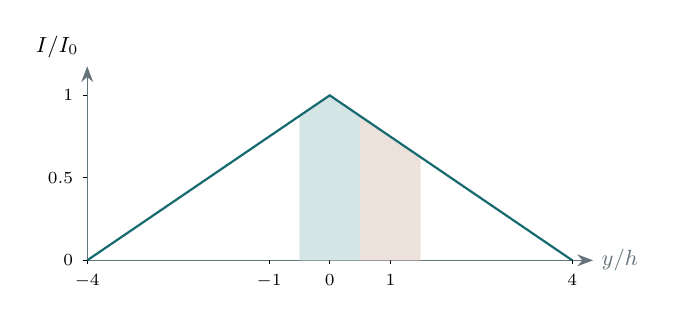
\begin{tikzpicture}[scale=.88,transform shape]
\draw[axis] (0,0.0)--(7.3,0.0) node[right] {$y/h$};
\draw[axis] (0,0)--(0,2.8);
\node[above left] at (0,2.8) {$I/I_0$};
\draw[thin] (0.000000,0.0)--(0.000000,-0.06);\node[below,font=\scriptsize] at (0.000000,-0.08) {$ -4 $};
\draw[thin] (2.625000,0.0)--(2.625000,-0.06);\node[below,font=\scriptsize] at (2.625000,-0.08) {$ -1 $};
\draw[thin] (3.500000,0.0)--(3.500000,-0.06);\node[below,font=\scriptsize] at (3.500000,-0.08) {$ 0 $};
\draw[thin] (4.375000,0.0)--(4.375000,-0.06);\node[below,font=\scriptsize] at (4.375000,-0.08) {$ 1 $};
\draw[thin] (7.000000,0.0)--(7.000000,-0.06);\node[below,font=\scriptsize] at (7.000000,-0.08) {$ 4 $};
\draw[thin] (0,0.000000)--(-.06,0.000000);\node[left,font=\scriptsize] at (-.08,0.000000) {$ 0 $};
\draw[thin] (0,1.190476)--(-.06,1.190476);\node[left,font=\scriptsize] at (-.08,1.190476) {$ 0.5 $};
\draw[thin] (0,2.380952)--(-.06,2.380952);\node[left,font=\scriptsize] at (-.08,2.380952) {$ 1 $};
\fill[accent!18] (3.0625000,0.0000000)--(3.0625000,2.0833333)--(3.5000000,2.3809524)--(3.9375000,2.0833333)--(3.9375000,0.0000000)--cycle;
\fill[warm!18] (3.9375000,0.0000000)--(3.9375000,2.0833333)--(4.8125000,1.4880952)--(4.8125000,0.0000000)--cycle;
\draw[thick,color=accent] plot coordinates {(0.0000000,0.0000000) (0.0291667,0.0198413) (0.0583333,0.0396825) (0.0875000,0.0595238) (0.1166667,0.0793651) (0.1458333,0.0992063) (0.1750000,0.1190476) (0.2041667,0.1388889) (0.2333333,0.1587302) (0.2625000,0.1785714) (0.2916667,0.1984127) (0.3208333,0.2182540) (0.3500000,0.2380952) (0.3791667,0.2579365) (0.4083333,0.2777778) (0.4375000,0.2976190) (0.4666667,0.3174603) (0.4958333,0.3373016) (0.5250000,0.3571429) (0.5541667,0.3769841) (0.5833333,0.3968254) (0.6125000,0.4166667) (0.6416667,0.4365079) (0.6708333,0.4563492) (0.7000000,0.4761905) (0.7291667,0.4960317) (0.7583333,0.5158730) (0.7875000,0.5357143) (0.8166667,0.5555556) (0.8458333,0.5753968) (0.8750000,0.5952381) (0.9041667,0.6150794) (0.9333333,0.6349206) (0.9625000,0.6547619) (0.9916667,0.6746032) (1.0208333,0.6944444) (1.0500000,0.7142857) (1.0791667,0.7341270) (1.1083333,0.7539683) (1.1375000,0.7738095) (1.1666667,0.7936508) (1.1958333,0.8134921) (1.2250000,0.8333333) (1.2541667,0.8531746) (1.2833333,0.8730159) (1.3125000,0.8928571) (1.3416667,0.9126984) (1.3708333,0.9325397) (1.4000000,0.9523810) (1.4291667,0.9722222) (1.4583333,0.9920635) (1.4875000,1.0119048) (1.5166667,1.0317460) (1.5458333,1.0515873) (1.5750000,1.0714286) (1.6041667,1.0912698) (1.6333333,1.1111111) (1.6625000,1.1309524) (1.6916667,1.1507937) (1.7208333,1.1706349) (1.7500000,1.1904762) (1.7791667,1.2103175) (1.8083333,1.2301587) (1.8375000,1.2500000) (1.8666667,1.2698413) (1.8958333,1.2896825) (1.9250000,1.3095238) (1.9541667,1.3293651) (1.9833333,1.3492063) (2.0125000,1.3690476) (2.0416667,1.3888889) (2.0708333,1.4087302) (2.1000000,1.4285714) (2.1291667,1.4484127) (2.1583333,1.4682540) (2.1875000,1.4880952) (2.2166667,1.5079365) (2.2458333,1.5277778) (2.2750000,1.5476190) (2.3041667,1.5674603) (2.3333333,1.5873016) (2.3625000,1.6071429) (2.3916667,1.6269841) (2.4208333,1.6468254) (2.4500000,1.6666667) (2.4791667,1.6865079) (2.5083333,1.7063492) (2.5375000,1.7261905) (2.5666667,1.7460317) (2.5958333,1.7658730) (2.6250000,1.7857143) (2.6541667,1.8055556) (2.6833333,1.8253968) (2.7125000,1.8452381) (2.7416667,1.8650794) (2.7708333,1.8849206) (2.8000000,1.9047619) (2.8291667,1.9246032) (2.8583333,1.9444444) (2.8875000,1.9642857) (2.9166667,1.9841270) (2.9458333,2.0039683) (2.9750000,2.0238095) (3.0041667,2.0436508) (3.0333333,2.0634921) (3.0625000,2.0833333) (3.0916667,2.1031746) (3.1208333,2.1230159) (3.1500000,2.1428571) (3.1791667,2.1626984) (3.2083333,2.1825397) (3.2375000,2.2023810) (3.2666667,2.2222222) (3.2958333,2.2420635) (3.3250000,2.2619048) (3.3541667,2.2817460) (3.3833333,2.3015873) (3.4125000,2.3214286) (3.4416667,2.3412698) (3.4708333,2.3611111) (3.5000000,2.3809524) (3.5291667,2.3611111) (3.5583333,2.3412698) (3.5875000,2.3214286) (3.6166667,2.3015873) (3.6458333,2.2817460) (3.6750000,2.2619048) (3.7041667,2.2420635) (3.7333333,2.2222222) (3.7625000,2.2023810) (3.7916667,2.1825397) (3.8208333,2.1626984) (3.8500000,2.1428571) (3.8791667,2.1230159) (3.9083333,2.1031746) (3.9375000,2.0833333) (3.9666667,2.0634921) (3.9958333,2.0436508) (4.0250000,2.0238095) (4.0541667,2.0039683) (4.0833333,1.9841270) (4.1125000,1.9642857) (4.1416667,1.9444444) (4.1708333,1.9246032) (4.2000000,1.9047619) (4.2291667,1.8849206) (4.2583333,1.8650794) (4.2875000,1.8452381) (4.3166667,1.8253968) (4.3458333,1.8055556) (4.3750000,1.7857143) (4.4041667,1.7658730) (4.4333333,1.7460317) (4.4625000,1.7261905) (4.4916667,1.7063492) (4.5208333,1.6865079) (4.5500000,1.6666667) (4.5791667,1.6468254) (4.6083333,1.6269841) (4.6375000,1.6071429) (4.6666667,1.5873016) (4.6958333,1.5674603) (4.7250000,1.5476190) (4.7541667,1.5277778) (4.7833333,1.5079365) (4.8125000,1.4880952) (4.8416667,1.4682540) (4.8708333,1.4484127) (4.9000000,1.4285714) (4.9291667,1.4087302) (4.9583333,1.3888889) (4.9875000,1.3690476) (5.0166667,1.3492063) (5.0458333,1.3293651) (5.0750000,1.3095238) (5.1041667,1.2896825) (5.1333333,1.2698413) (5.1625000,1.2500000) (5.1916667,1.2301587) (5.2208333,1.2103175) (5.2500000,1.1904762) (5.2791667,1.1706349) (5.3083333,1.1507937) (5.3375000,1.1309524) (5.3666667,1.1111111) (5.3958333,1.0912698) (5.4250000,1.0714286) (5.4541667,1.0515873) (5.4833333,1.0317460) (5.5125000,1.0119048) (5.5416667,0.9920635) (5.5708333,0.9722222) (5.6000000,0.9523810) (5.6291667,0.9325397) (5.6583333,0.9126984) (5.6875000,0.8928571) (5.7166667,0.8730159) (5.7458333,0.8531746) (5.7750000,0.8333333) (5.8041667,0.8134921) (5.8333333,0.7936508) (5.8625000,0.7738095) (5.8916667,0.7539683) (5.9208333,0.7341270) (5.9500000,0.7142857) (5.9791667,0.6944444) (6.0083333,0.6746032) (6.0375000,0.6547619) (6.0666667,0.6349206) (6.0958333,0.6150794) (6.1250000,0.5952381) (6.1541667,0.5753968) (6.1833333,0.5555556) (6.2125000,0.5357143) (6.2416667,0.5158730) (6.2708333,0.4960317) (6.3000000,0.4761905) (6.3291667,0.4563492) (6.3583333,0.4365079) (6.3875000,0.4166667) (6.4166667,0.3968254) (6.4458333,0.3769841) (6.4750000,0.3571429) (6.5041667,0.3373016) (6.5333333,0.3174603) (6.5625000,0.2976190) (6.5916667,0.2777778) (6.6208333,0.2579365) (6.6500000,0.2380952) (6.6791667,0.2182540) (6.7083333,0.1984127) (6.7375000,0.1785714) (6.7666667,0.1587302) (6.7958333,0.1388889) (6.8250000,0.1190476) (6.8541667,0.0992063) (6.8833333,0.0793651) (6.9125000,0.0595238) (6.9416667,0.0396825) (6.9708333,0.0198413) (7.0000000,0.0000000)};
\end{tikzpicture}
\figcaption{解图近1.2B\quad u等于1/2时，下条带负半到正半，上条带全在正半}
\end{minipage}\end{center}
令$u=y_0/h$，先计算正位移。$0\le u\le1$时，上条带全在正半轴，故
\[
 \frac{P_u}{hwI_0}=\int_u^{u+1}(1-v/4)\dd v
 =1-\frac{(u+1)^2-u^2}{8}=\frac78-\frac u4.
\]
下条带跨过光强尖点$v=0$，分别积分两侧线性函数：
\[
 \frac{P_l}{hwI_0}
 =\int_{u-1}^0(1+v/4)\dd v+\int_0^u(1-v/4)\dd v
 =\left(1-u-\frac{(1-u)^2}{8}\right)
  +\left(u-\frac{u^2}{8}\right).
\]
这两段也对应图中各自的平均照度：负半段长$h(1-u)$、中点为$-h(1-u)/2$，其平均光强为$I_0(7/8+u/8)$；正半段长$hu$、中点为$hu/2$，平均光强为$I_0(1-u/8)$。乘上各段投影面积后相加，即
\[
 P_l=hwI_0\left[(1-u)\left(\frac78+\frac u8\right)
 +u\left(1-\frac u8\right)\right].
\]
这正是上面积分中两个区间的面积，合并得到
\[
\frac{P_u}{hwI_0}=\frac78-\frac u4,\qquad
\frac{P_l}{hwI_0}=\frac78+\frac u4-\frac{u^2}4.
\]
这也可用两小段各自的中点光强乘长度，权重分别为$1-u$与$u$；整条跨零条带使用上面的两段平均。此时功率和为$hwI_0(7/4-u^2/4)$，功率差为$-hwI_0(u/2-u^2/4)$。

$1\le u\le3$时，两条带都在正半轴，每条带内光强均为线性函数，平均值等于各自中点值$I(y_0\pm h/2)$，因此
\[
\frac{P_u}{hwI_0}=\frac78-\frac u4,\quad
\frac{P_l}{hwI_0}=\frac98-\frac u4.
\]
功率和为$hwI_0(2-u/2)$，差为$-hwI_0/4$。两条相邻等宽带随棱镜一起平移，在线性光强段内，它们的平均值始终相差$I_0/4$，所以外段竖直力保持常量；两条带的总照度却随高度减小，水平力仍变化。关于$y=0$的光强对称使$P_u(-u)=P_l(u)$，所以水平方向力为偶函数、竖直方向力为奇函数。整个指定区间的结果为
\[
\boxed{\frac{cF_x}{hwI_0(1-\cos\theta)}
=\begin{cases}7/4-u^2/4,&|u|\leqslant1,\\2-|u|/2,&1\leqslant|u|\leqslant3,\end{cases}}
\]
\[
\boxed{\frac{cF_y}{hwI_0\sin\theta}
=\begin{cases}-\dfrac u2(1-\dfrac{|u|}2),&|u|\leqslant1,\\
-\dfrac{\operatorname{sgn}u}{4},&1\leqslant|u|\leqslant3.\end{cases}}
\]
解图近1.2C画两条分段函数。在$u=0$，水平系数为$7/4$、竖直力为零；在$|u|=1$，水平系数为$3/2$，竖直系数为$\mp1/4$，两段连续衔接；在$|u|=3$，水平系数仍为$1/2$。外段水平力随$|u|$线性下降，竖直力为回复方向的常量。它们由条带积分的区间变化给出。
\begin{center}\begin{minipage}{.98\linewidth}\centering
\begin{tikzpicture}[scale=.88,transform shape]
\draw[axis] (0,0.3488372093023256)--(7.3,0.3488372093023256) node[right] {$u=y_0/h$};
\draw[axis] (0,0)--(0,2.8);
\node[above left] at (0,2.8) {归一化光力};
\draw[thin] (0.000000,0.3488372093023256)--(0.000000,0.2888372093023256);\node[below,font=\scriptsize] at (0.000000,0.2688372093023256) {$ -3 $};
\draw[thin] (2.333333,0.3488372093023256)--(2.333333,0.2888372093023256);\node[below,font=\scriptsize] at (2.333333,0.2688372093023256) {$ -1 $};
\draw[thin] (3.500000,0.3488372093023256)--(3.500000,0.2888372093023256);\node[below,font=\scriptsize] at (3.500000,0.2688372093023256) {$ 0 $};
\draw[thin] (4.666667,0.3488372093023256)--(4.666667,0.2888372093023256);\node[below,font=\scriptsize] at (4.666667,0.2688372093023256) {$ 1 $};
\draw[thin] (7.000000,0.3488372093023256)--(7.000000,0.2888372093023256);\node[below,font=\scriptsize] at (7.000000,0.2688372093023256) {$ 3 $};
\draw[thin] (0,0.058140)--(-.06,0.058140);\node[left,font=\scriptsize] at (-.08,0.058140) {$ -0.25 $};
\draw[thin] (0,0.348837)--(-.06,0.348837);\node[left,font=\scriptsize] at (-.08,0.348837) {$ 0 $};
\draw[thin] (0,0.930233)--(-.06,0.930233);\node[left,font=\scriptsize] at (-.08,0.930233) {$ 0.5 $};
\draw[thin] (0,2.093023)--(-.06,2.093023);\node[left,font=\scriptsize] at (-.08,2.093023) {$ 1.5 $};
\draw[thin] (0,2.383721)--(-.06,2.383721);\node[left,font=\scriptsize] at (-.08,2.383721) {$ 1.75 $};
\draw[thick,color=accent] plot coordinates {(0.0000000,0.9302326) (0.0291667,0.9447674) (0.0583333,0.9593023) (0.0875000,0.9738372) (0.1166667,0.9883721) (0.1458333,1.0029070) (0.1750000,1.0174419) (0.2041667,1.0319767) (0.2333333,1.0465116) (0.2625000,1.0610465) (0.2916667,1.0755814) (0.3208333,1.0901163) (0.3500000,1.1046512) (0.3791667,1.1191860) (0.4083333,1.1337209) (0.4375000,1.1482558) (0.4666667,1.1627907) (0.4958333,1.1773256) (0.5250000,1.1918605) (0.5541667,1.2063953) (0.5833333,1.2209302) (0.6125000,1.2354651) (0.6416667,1.2500000) (0.6708333,1.2645349) (0.7000000,1.2790698) (0.7291667,1.2936047) (0.7583333,1.3081395) (0.7875000,1.3226744) (0.8166667,1.3372093) (0.8458333,1.3517442) (0.8750000,1.3662791) (0.9041667,1.3808140) (0.9333333,1.3953488) (0.9625000,1.4098837) (0.9916667,1.4244186) (1.0208333,1.4389535) (1.0500000,1.4534884) (1.0791667,1.4680233) (1.1083333,1.4825581) (1.1375000,1.4970930) (1.1666667,1.5116279) (1.1958333,1.5261628) (1.2250000,1.5406977) (1.2541667,1.5552326) (1.2833333,1.5697674) (1.3125000,1.5843023) (1.3416667,1.5988372) (1.3708333,1.6133721) (1.4000000,1.6279070) (1.4291667,1.6424419) (1.4583333,1.6569767) (1.4875000,1.6715116) (1.5166667,1.6860465) (1.5458333,1.7005814) (1.5750000,1.7151163) (1.6041667,1.7296512) (1.6333333,1.7441860) (1.6625000,1.7587209) (1.6916667,1.7732558) (1.7208333,1.7877907) (1.7500000,1.8023256) (1.7791667,1.8168605) (1.8083333,1.8313953) (1.8375000,1.8459302) (1.8666667,1.8604651) (1.8958333,1.8750000) (1.9250000,1.8895349) (1.9541667,1.9040698) (1.9833333,1.9186047) (2.0125000,1.9331395) (2.0416667,1.9476744) (2.0708333,1.9622093) (2.1000000,1.9767442) (2.1291667,1.9912791) (2.1583333,2.0058140) (2.1875000,2.0203488) (2.2166667,2.0348837) (2.2458333,2.0494186) (2.2750000,2.0639535) (2.3041667,2.0784884) (2.3333333,2.0930233) (2.3625000,2.1073765) (2.3916667,2.1213663) (2.4208333,2.1349927) (2.4500000,2.1482558) (2.4791667,2.1611555) (2.5083333,2.1736919) (2.5375000,2.1858648) (2.5666667,2.1976744) (2.5958333,2.2091206) (2.6250000,2.2202035) (2.6541667,2.2309230) (2.6833333,2.2412791) (2.7125000,2.2512718) (2.7416667,2.2609012) (2.7708333,2.2701672) (2.8000000,2.2790698) (2.8291667,2.2876090) (2.8583333,2.2957849) (2.8875000,2.3035974) (2.9166667,2.3110465) (2.9458333,2.3181323) (2.9750000,2.3248547) (3.0041667,2.3312137) (3.0333333,2.3372093) (3.0625000,2.3428416) (3.0916667,2.3481105) (3.1208333,2.3530160) (3.1500000,2.3575581) (3.1791667,2.3617369) (3.2083333,2.3655523) (3.2375000,2.3690044) (3.2666667,2.3720930) (3.2958333,2.3748183) (3.3250000,2.3771802) (3.3541667,2.3791788) (3.3833333,2.3808140) (3.4125000,2.3820858) (3.4416667,2.3829942) (3.4708333,2.3835392) (3.5000000,2.3837209) (3.5291667,2.3835392) (3.5583333,2.3829942) (3.5875000,2.3820858) (3.6166667,2.3808140) (3.6458333,2.3791788) (3.6750000,2.3771802) (3.7041667,2.3748183) (3.7333333,2.3720930) (3.7625000,2.3690044) (3.7916667,2.3655523) (3.8208333,2.3617369) (3.8500000,2.3575581) (3.8791667,2.3530160) (3.9083333,2.3481105) (3.9375000,2.3428416) (3.9666667,2.3372093) (3.9958333,2.3312137) (4.0250000,2.3248547) (4.0541667,2.3181323) (4.0833333,2.3110465) (4.1125000,2.3035974) (4.1416667,2.2957849) (4.1708333,2.2876090) (4.2000000,2.2790698) (4.2291667,2.2701672) (4.2583333,2.2609012) (4.2875000,2.2512718) (4.3166667,2.2412791) (4.3458333,2.2309230) (4.3750000,2.2202035) (4.4041667,2.2091206) (4.4333333,2.1976744) (4.4625000,2.1858648) (4.4916667,2.1736919) (4.5208333,2.1611555) (4.5500000,2.1482558) (4.5791667,2.1349927) (4.6083333,2.1213663) (4.6375000,2.1073765) (4.6666667,2.0930233) (4.6958333,2.0784884) (4.7250000,2.0639535) (4.7541667,2.0494186) (4.7833333,2.0348837) (4.8125000,2.0203488) (4.8416667,2.0058140) (4.8708333,1.9912791) (4.9000000,1.9767442) (4.9291667,1.9622093) (4.9583333,1.9476744) (4.9875000,1.9331395) (5.0166667,1.9186047) (5.0458333,1.9040698) (5.0750000,1.8895349) (5.1041667,1.8750000) (5.1333333,1.8604651) (5.1625000,1.8459302) (5.1916667,1.8313953) (5.2208333,1.8168605) (5.2500000,1.8023256) (5.2791667,1.7877907) (5.3083333,1.7732558) (5.3375000,1.7587209) (5.3666667,1.7441860) (5.3958333,1.7296512) (5.4250000,1.7151163) (5.4541667,1.7005814) (5.4833333,1.6860465) (5.5125000,1.6715116) (5.5416667,1.6569767) (5.5708333,1.6424419) (5.6000000,1.6279070) (5.6291667,1.6133721) (5.6583333,1.5988372) (5.6875000,1.5843023) (5.7166667,1.5697674) (5.7458333,1.5552326) (5.7750000,1.5406977) (5.8041667,1.5261628) (5.8333333,1.5116279) (5.8625000,1.4970930) (5.8916667,1.4825581) (5.9208333,1.4680233) (5.9500000,1.4534884) (5.9791667,1.4389535) (6.0083333,1.4244186) (6.0375000,1.4098837) (6.0666667,1.3953488) (6.0958333,1.3808140) (6.1250000,1.3662791) (6.1541667,1.3517442) (6.1833333,1.3372093) (6.2125000,1.3226744) (6.2416667,1.3081395) (6.2708333,1.2936047) (6.3000000,1.2790698) (6.3291667,1.2645349) (6.3583333,1.2500000) (6.3875000,1.2354651) (6.4166667,1.2209302) (6.4458333,1.2063953) (6.4750000,1.1918605) (6.5041667,1.1773256) (6.5333333,1.1627907) (6.5625000,1.1482558) (6.5916667,1.1337209) (6.6208333,1.1191860) (6.6500000,1.1046512) (6.6791667,1.0901163) (6.7083333,1.0755814) (6.7375000,1.0610465) (6.7666667,1.0465116) (6.7958333,1.0319767) (6.8250000,1.0174419) (6.8541667,1.0029070) (6.8833333,0.9883721) (6.9125000,0.9738372) (6.9416667,0.9593023) (6.9708333,0.9447674) (7.0000000,0.9302326)};
\draw[thick,color=accent] (7.65,2.55)--(8.15,2.55);\node[right,font=\scriptsize] at (8.2,2.55) {$cF_x/[hwI_0(1-\cos\theta)]$};
\draw[thick,dashed,color=warm] plot coordinates {(0.0000000,0.6395349) (0.0291667,0.6395349) (0.0583333,0.6395349) (0.0875000,0.6395349) (0.1166667,0.6395349) (0.1458333,0.6395349) (0.1750000,0.6395349) (0.2041667,0.6395349) (0.2333333,0.6395349) (0.2625000,0.6395349) (0.2916667,0.6395349) (0.3208333,0.6395349) (0.3500000,0.6395349) (0.3791667,0.6395349) (0.4083333,0.6395349) (0.4375000,0.6395349) (0.4666667,0.6395349) (0.4958333,0.6395349) (0.5250000,0.6395349) (0.5541667,0.6395349) (0.5833333,0.6395349) (0.6125000,0.6395349) (0.6416667,0.6395349) (0.6708333,0.6395349) (0.7000000,0.6395349) (0.7291667,0.6395349) (0.7583333,0.6395349) (0.7875000,0.6395349) (0.8166667,0.6395349) (0.8458333,0.6395349) (0.8750000,0.6395349) (0.9041667,0.6395349) (0.9333333,0.6395349) (0.9625000,0.6395349) (0.9916667,0.6395349) (1.0208333,0.6395349) (1.0500000,0.6395349) (1.0791667,0.6395349) (1.1083333,0.6395349) (1.1375000,0.6395349) (1.1666667,0.6395349) (1.1958333,0.6395349) (1.2250000,0.6395349) (1.2541667,0.6395349) (1.2833333,0.6395349) (1.3125000,0.6395349) (1.3416667,0.6395349) (1.3708333,0.6395349) (1.4000000,0.6395349) (1.4291667,0.6395349) (1.4583333,0.6395349) (1.4875000,0.6395349) (1.5166667,0.6395349) (1.5458333,0.6395349) (1.5750000,0.6395349) (1.6041667,0.6395349) (1.6333333,0.6395349) (1.6625000,0.6395349) (1.6916667,0.6395349) (1.7208333,0.6395349) (1.7500000,0.6395349) (1.7791667,0.6395349) (1.8083333,0.6395349) (1.8375000,0.6395349) (1.8666667,0.6395349) (1.8958333,0.6395349) (1.9250000,0.6395349) (1.9541667,0.6395349) (1.9833333,0.6395349) (2.0125000,0.6395349) (2.0416667,0.6395349) (2.0708333,0.6395349) (2.1000000,0.6395349) (2.1291667,0.6395349) (2.1583333,0.6395349) (2.1875000,0.6395349) (2.2166667,0.6395349) (2.2458333,0.6395349) (2.2750000,0.6395349) (2.3041667,0.6395349) (2.3333333,0.6395349) (2.3625000,0.6393532) (2.3916667,0.6388081) (2.4208333,0.6378997) (2.4500000,0.6366279) (2.4791667,0.6349927) (2.5083333,0.6329942) (2.5375000,0.6306323) (2.5666667,0.6279070) (2.5958333,0.6248183) (2.6250000,0.6213663) (2.6541667,0.6175509) (2.6833333,0.6133721) (2.7125000,0.6088299) (2.7416667,0.6039244) (2.7708333,0.5986555) (2.8000000,0.5930233) (2.8291667,0.5870276) (2.8583333,0.5806686) (2.8875000,0.5739462) (2.9166667,0.5668605) (2.9458333,0.5594113) (2.9750000,0.5515988) (3.0041667,0.5434230) (3.0333333,0.5348837) (3.0625000,0.5259811) (3.0916667,0.5167151) (3.1208333,0.5070858) (3.1500000,0.4970930) (3.1791667,0.4867369) (3.2083333,0.4760174) (3.2375000,0.4649346) (3.2666667,0.4534884) (3.2958333,0.4416788) (3.3250000,0.4295058) (3.3541667,0.4169695) (3.3833333,0.4040698) (3.4125000,0.3908067) (3.4416667,0.3771802) (3.4708333,0.3631904) (3.5000000,0.3488372) (3.5291667,0.3344840) (3.5583333,0.3204942) (3.5875000,0.3068677) (3.6166667,0.2936047) (3.6458333,0.2807049) (3.6750000,0.2681686) (3.7041667,0.2559956) (3.7333333,0.2441860) (3.7625000,0.2327398) (3.7916667,0.2216570) (3.8208333,0.2109375) (3.8500000,0.2005814) (3.8791667,0.1905887) (3.9083333,0.1809593) (3.9375000,0.1716933) (3.9666667,0.1627907) (3.9958333,0.1542515) (4.0250000,0.1460756) (4.0541667,0.1382631) (4.0833333,0.1308140) (4.1125000,0.1237282) (4.1416667,0.1170058) (4.1708333,0.1106468) (4.2000000,0.1046512) (4.2291667,0.0990189) (4.2583333,0.0937500) (4.2875000,0.0888445) (4.3166667,0.0843023) (4.3458333,0.0801235) (4.3750000,0.0763081) (4.4041667,0.0728561) (4.4333333,0.0697674) (4.4625000,0.0670422) (4.4916667,0.0646802) (4.5208333,0.0626817) (4.5500000,0.0610465) (4.5791667,0.0597747) (4.6083333,0.0588663) (4.6375000,0.0583212) (4.6666667,0.0581395) (4.6958333,0.0581395) (4.7250000,0.0581395) (4.7541667,0.0581395) (4.7833333,0.0581395) (4.8125000,0.0581395) (4.8416667,0.0581395) (4.8708333,0.0581395) (4.9000000,0.0581395) (4.9291667,0.0581395) (4.9583333,0.0581395) (4.9875000,0.0581395) (5.0166667,0.0581395) (5.0458333,0.0581395) (5.0750000,0.0581395) (5.1041667,0.0581395) (5.1333333,0.0581395) (5.1625000,0.0581395) (5.1916667,0.0581395) (5.2208333,0.0581395) (5.2500000,0.0581395) (5.2791667,0.0581395) (5.3083333,0.0581395) (5.3375000,0.0581395) (5.3666667,0.0581395) (5.3958333,0.0581395) (5.4250000,0.0581395) (5.4541667,0.0581395) (5.4833333,0.0581395) (5.5125000,0.0581395) (5.5416667,0.0581395) (5.5708333,0.0581395) (5.6000000,0.0581395) (5.6291667,0.0581395) (5.6583333,0.0581395) (5.6875000,0.0581395) (5.7166667,0.0581395) (5.7458333,0.0581395) (5.7750000,0.0581395) (5.8041667,0.0581395) (5.8333333,0.0581395) (5.8625000,0.0581395) (5.8916667,0.0581395) (5.9208333,0.0581395) (5.9500000,0.0581395) (5.9791667,0.0581395) (6.0083333,0.0581395) (6.0375000,0.0581395) (6.0666667,0.0581395) (6.0958333,0.0581395) (6.1250000,0.0581395) (6.1541667,0.0581395) (6.1833333,0.0581395) (6.2125000,0.0581395) (6.2416667,0.0581395) (6.2708333,0.0581395) (6.3000000,0.0581395) (6.3291667,0.0581395) (6.3583333,0.0581395) (6.3875000,0.0581395) (6.4166667,0.0581395) (6.4458333,0.0581395) (6.4750000,0.0581395) (6.5041667,0.0581395) (6.5333333,0.0581395) (6.5625000,0.0581395) (6.5916667,0.0581395) (6.6208333,0.0581395) (6.6500000,0.0581395) (6.6791667,0.0581395) (6.7083333,0.0581395) (6.7375000,0.0581395) (6.7666667,0.0581395) (6.7958333,0.0581395) (6.8250000,0.0581395) (6.8541667,0.0581395) (6.8833333,0.0581395) (6.9125000,0.0581395) (6.9416667,0.0581395) (6.9708333,0.0581395) (7.0000000,0.0581395)};
\draw[thick,dashed,color=warm] (7.65,2.0999999999999996)--(8.15,2.0999999999999996);\node[right,font=\scriptsize] at (8.2,2.0999999999999996) {$cF_y/(hwI_0\sin\theta)$};
\end{tikzpicture}
\figcaption{解图近1.2C\quad 完整分段光力在中央与外段连续衔接}
\end{minipage}\end{center}
（3）代$\alpha=30^\circ,n=1.5$，先得$\beta=19.4712^\circ$，内部光线对底面法线的夹角为$10.5288^\circ$，第二次折射得到$\theta=15.9080^\circ$。三角形横截面的底边为$2h$，沿$x$的高为$h\tan\alpha$，所以截面积为$h^2\tan\alpha$，乘厚度$w$后得到
\[
V=h^2w\tan\alpha,\quad m=\rho h^2w\tan\alpha=1.4434\times10^{-10}\,\mathrm{kg},
\quad \theta=15.9080^\circ.
\]
这里$h=10^{-5}\,\mathrm m,w=10^{-3}\,\mathrm m,\rho=2.5\times10^3\,\mathrm{kg/m^3}$，质量为$1.4434\times10^{-10}\,\mathrm{kg}$，取$g=9.8\,\mathrm{m/s^2}$时重力约$1.4145\times10^{-9}\,\mathrm N$。在$u=-1/2$处，竖直分段系数为$1/4-1/16=3/16$，因而$F_y=3hwI_0\sin\theta/(16c)$。令它与重力相等，
\[
I_0=\frac{16cmg}{3hw\sin\theta}\simeq8.26\times10^8\,\mathrm{W/m^2}.
\]
接下来求整束光功率。其宽度为$8h$，光强剖面的三角形面积为$\tfrac12(8h)I_0=4hI_0$，再乘沿$z$的宽度$w$，所以
\[
\boxed{P=w\int_{-4h}^{4h}I(y)\dd y=4hwI_0\simeq33.0\,\mathrm W}.
\]
棱镜仅截获其中一部分光，激光器总功率使用整个$-4h$到$4h$范围。上述等式给竖直平衡，水平方向的$F_x$仍为正。在该偏移处，水平分段系数为$7/4-(1/2)^2/4=27/16$，因此
\[
 \frac{F_x}{mg}=\frac{27(1-\cos\theta)}{3\sin\theta}
 =9\tan\frac{\theta}{2}.
\]
这项前进力与已平衡的竖直分量具有相同光功率尺度。要求棱镜整体静止时，另以水平约束或对向光束配平；若只释放竖直自由度，便在对应偏移处讨论竖直平衡。

（4）本问去掉重力，并取$I_0=10^8\,\mathrm{W/m^2}$，区别于上一问重力平衡所需的峰值。中心段的完整竖直力为
\[
 F_y=-\frac{wI_0\sin\theta}{2c}\,y
 \left(1-\frac{|y|}{2h}\right),\qquad |y|\le h.
\]
在$y=0$附近，线性项为$-Ky$，从质量和该系数得到
\[
K=\frac{wI_0\sin\theta}{2c},\quad
m\ddot y+Ky\simeq0,\quad
\boxed{T_0=2\pi\sqrt{\frac mK}
=2\pi\sqrt{\frac{2c\rho h^2\tan\alpha}{I_0\sin\theta}}
\simeq1.117\times10^{-2}\,\mathrm s}.
\]
解图近1.2D把实际回复势与线性抛物线放在一起。指定振幅$a=h/20$，全程$|y|/(2h)\le0.025$，故上式的非线性项是小修正，$T_0$为小振动周期。振动方向的能量由$\dd U/\dd y=-F_y$给出：对正$y$积分并按偶对称延伸，
\[
U(y)=\frac K2y^2-\frac{K}{6h}|y|^3,\qquad
T(a)=4\sqrt{\frac m2}\int_0^a\frac{\dd y}{\sqrt{U(a)-U(y)}}.
\]
其中$U(0)=0$，总竖直能量为$U(a)$，$m\dot y^2/2=U(a)-U(y)$。从中心积分到转折点的时间为一个周期的四分之一，因而得到上面的有限振幅周期式。解图近1.2D中$|y|^3$项使势能曲线低于抛物线，振幅增加时周期略长。令$y=a\sin\psi$，将转折点处的平方根因子提出，得
\[
 \frac{T(a)}{T_0}=\frac2\pi\int_0^{\pi/2}
 \left[1-\frac{a}{3h}\frac{1-\sin^3\psi}{1-\sin^2\psi}\right]^{-1/2}\dd\psi.
\]
括号内的比值写成$\sin\psi+1/(1+\sin\psi)$，在$\psi=\pi/2$处按连续值取$3/2$。利用
\[
 \int_0^{\pi/2}\sin\psi\,\dd\psi=1,\qquad
 \int_0^{\pi/2}\frac{\dd\psi}{1+\sin\psi}
 =\left[-\frac{\cos\psi}{1+\sin\psi}\right]_0^{\pi/2}=1,
\]
将被积式按$a/h$展开到一阶，便有
\[
 \frac{T(a)}{T_0}=1+\frac{2a}{3\pi h}
 +O\!\left(\frac{a^2}{h^2}\right).
\]
因此$a=h/20$时，首阶周期增加约$1.061\%$；完整能量积分给$T(a)/T_0\simeq1.01079$。线性周期与有限振幅周期都由同一条回复势得到，图中的软化项决定这项差别。
\begin{center}\begin{minipage}{.98\linewidth}\centering
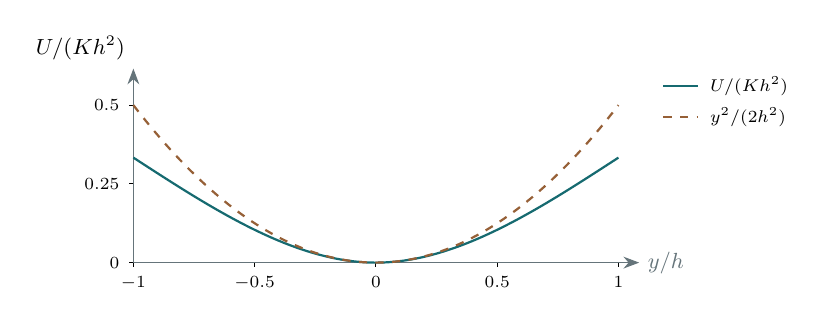
\begin{tikzpicture}[scale=.88,transform shape]
\draw[axis] (0,0.0)--(7.3,0.0) node[right] {$y/h$};
\draw[axis] (0,0)--(0,2.8);
\node[above left] at (0,2.8) {$U/(Kh^2)$};
\draw[thin] (0.000000,0.0)--(0.000000,-0.06);\node[below,font=\scriptsize] at (0.000000,-0.08) {$ -1 $};
\draw[thin] (1.750000,0.0)--(1.750000,-0.06);\node[below,font=\scriptsize] at (1.750000,-0.08) {$ -0.5 $};
\draw[thin] (3.500000,0.0)--(3.500000,-0.06);\node[below,font=\scriptsize] at (3.500000,-0.08) {$ 0 $};
\draw[thin] (5.250000,0.0)--(5.250000,-0.06);\node[below,font=\scriptsize] at (5.250000,-0.08) {$ 0.5 $};
\draw[thin] (7.000000,0.0)--(7.000000,-0.06);\node[below,font=\scriptsize] at (7.000000,-0.08) {$ 1 $};
\draw[thin] (0,0.000000)--(-.06,0.000000);\node[left,font=\scriptsize] at (-.08,0.000000) {$ 0 $};
\draw[thin] (0,1.136364)--(-.06,1.136364);\node[left,font=\scriptsize] at (-.08,1.136364) {$ 0.25 $};
\draw[thin] (0,2.272727)--(-.06,2.272727);\node[left,font=\scriptsize] at (-.08,2.272727) {$ 0.5 $};
\draw[thick,color=accent] plot coordinates {(0.0000000,1.5151515) (0.0291667,1.4962126) (0.0583333,1.4772762) (0.0875000,1.4583452) (0.1166667,1.4394220) (0.1458333,1.4205093) (0.1750000,1.4016098) (0.2041667,1.3827261) (0.2333333,1.3638608) (0.2625000,1.3450166) (0.2916667,1.3261960) (0.3208333,1.3074017) (0.3500000,1.2886364) (0.3791667,1.2699026) (0.4083333,1.2512030) (0.4375000,1.2325402) (0.4666667,1.2139169) (0.4958333,1.1953357) (0.5250000,1.1767992) (0.5541667,1.1583101) (0.5833333,1.1398709) (0.6125000,1.1214844) (0.6416667,1.1031531) (0.6708333,1.0848796) (0.7000000,1.0666667) (0.7291667,1.0485169) (0.7583333,1.0304328) (0.7875000,1.0124171) (0.8166667,0.9944725) (0.8458333,0.9766015) (0.8750000,0.9588068) (0.9041667,0.9410910) (0.9333333,0.9234568) (0.9625000,0.9059067) (0.9916667,0.8884435) (1.0208333,0.8710696) (1.0500000,0.8537879) (1.0791667,0.8366008) (1.1083333,0.8195111) (1.1375000,0.8025213) (1.1666667,0.7856341) (1.1958333,0.7688521) (1.2250000,0.7521780) (1.2541667,0.7356144) (1.2833333,0.7191639) (1.3125000,0.7028291) (1.3416667,0.6866127) (1.3708333,0.6705172) (1.4000000,0.6545455) (1.4291667,0.6386999) (1.4583333,0.6229833) (1.4875000,0.6073982) (1.5166667,0.5919473) (1.5458333,0.5766331) (1.5750000,0.5614583) (1.6041667,0.5464256) (1.6333333,0.5315376) (1.6625000,0.5167969) (1.6916667,0.5022061) (1.7208333,0.4877679) (1.7500000,0.4734848) (1.7791667,0.4593597) (1.8083333,0.4453949) (1.8375000,0.4315933) (1.8666667,0.4179574) (1.8958333,0.4044898) (1.9250000,0.3911932) (1.9541667,0.3780702) (1.9833333,0.3651235) (2.0125000,0.3523556) (2.0416667,0.3397692) (2.0708333,0.3273670) (2.1000000,0.3151515) (2.1291667,0.3031254) (2.1583333,0.2912914) (2.1875000,0.2796520) (2.2166667,0.2682099) (2.2458333,0.2569677) (2.2750000,0.2459280) (2.3041667,0.2350936) (2.3333333,0.2244669) (2.3625000,0.2140507) (2.3916667,0.2038475) (2.4208333,0.1938600) (2.4500000,0.1840909) (2.4791667,0.1745427) (2.5083333,0.1652182) (2.5375000,0.1561198) (2.5666667,0.1472503) (2.5958333,0.1386123) (2.6250000,0.1302083) (2.6541667,0.1220412) (2.6833333,0.1141134) (2.7125000,0.1064276) (2.7416667,0.0989864) (2.7708333,0.0917925) (2.8000000,0.0848485) (2.8291667,0.0781570) (2.8583333,0.0717207) (2.8875000,0.0655421) (2.9166667,0.0596240) (2.9458333,0.0539689) (2.9750000,0.0485795) (3.0041667,0.0434585) (3.0333333,0.0386083) (3.0625000,0.0340317) (3.0916667,0.0297313) (3.1208333,0.0257098) (3.1500000,0.0219697) (3.1791667,0.0185137) (3.2083333,0.0153444) (3.2375000,0.0124645) (3.2666667,0.0098765) (3.2958333,0.0075832) (3.3250000,0.0055871) (3.3541667,0.0038909) (3.3833333,0.0024972) (3.4125000,0.0014086) (3.4416667,0.0006278) (3.4708333,0.0001574) (3.5000000,0.0000000) (3.5291667,0.0001574) (3.5583333,0.0006278) (3.5875000,0.0014086) (3.6166667,0.0024972) (3.6458333,0.0038909) (3.6750000,0.0055871) (3.7041667,0.0075832) (3.7333333,0.0098765) (3.7625000,0.0124645) (3.7916667,0.0153444) (3.8208333,0.0185137) (3.8500000,0.0219697) (3.8791667,0.0257098) (3.9083333,0.0297313) (3.9375000,0.0340317) (3.9666667,0.0386083) (3.9958333,0.0434585) (4.0250000,0.0485795) (4.0541667,0.0539689) (4.0833333,0.0596240) (4.1125000,0.0655421) (4.1416667,0.0717207) (4.1708333,0.0781570) (4.2000000,0.0848485) (4.2291667,0.0917925) (4.2583333,0.0989864) (4.2875000,0.1064276) (4.3166667,0.1141134) (4.3458333,0.1220412) (4.3750000,0.1302083) (4.4041667,0.1386123) (4.4333333,0.1472503) (4.4625000,0.1561198) (4.4916667,0.1652182) (4.5208333,0.1745427) (4.5500000,0.1840909) (4.5791667,0.1938600) (4.6083333,0.2038475) (4.6375000,0.2140507) (4.6666667,0.2244669) (4.6958333,0.2350936) (4.7250000,0.2459280) (4.7541667,0.2569677) (4.7833333,0.2682099) (4.8125000,0.2796520) (4.8416667,0.2912914) (4.8708333,0.3031254) (4.9000000,0.3151515) (4.9291667,0.3273670) (4.9583333,0.3397692) (4.9875000,0.3523556) (5.0166667,0.3651235) (5.0458333,0.3780702) (5.0750000,0.3911932) (5.1041667,0.4044898) (5.1333333,0.4179574) (5.1625000,0.4315933) (5.1916667,0.4453949) (5.2208333,0.4593597) (5.2500000,0.4734848) (5.2791667,0.4877679) (5.3083333,0.5022061) (5.3375000,0.5167969) (5.3666667,0.5315376) (5.3958333,0.5464256) (5.4250000,0.5614583) (5.4541667,0.5766331) (5.4833333,0.5919473) (5.5125000,0.6073982) (5.5416667,0.6229833) (5.5708333,0.6386999) (5.6000000,0.6545455) (5.6291667,0.6705172) (5.6583333,0.6866127) (5.6875000,0.7028291) (5.7166667,0.7191639) (5.7458333,0.7356144) (5.7750000,0.7521780) (5.8041667,0.7688521) (5.8333333,0.7856341) (5.8625000,0.8025213) (5.8916667,0.8195111) (5.9208333,0.8366008) (5.9500000,0.8537879) (5.9791667,0.8710696) (6.0083333,0.8884435) (6.0375000,0.9059067) (6.0666667,0.9234568) (6.0958333,0.9410910) (6.1250000,0.9588068) (6.1541667,0.9766015) (6.1833333,0.9944725) (6.2125000,1.0124171) (6.2416667,1.0304328) (6.2708333,1.0485169) (6.3000000,1.0666667) (6.3291667,1.0848796) (6.3583333,1.1031531) (6.3875000,1.1214844) (6.4166667,1.1398709) (6.4458333,1.1583101) (6.4750000,1.1767992) (6.5041667,1.1953357) (6.5333333,1.2139169) (6.5625000,1.2325402) (6.5916667,1.2512030) (6.6208333,1.2699026) (6.6500000,1.2886364) (6.6791667,1.3074017) (6.7083333,1.3261960) (6.7375000,1.3450166) (6.7666667,1.3638608) (6.7958333,1.3827261) (6.8250000,1.4016098) (6.8541667,1.4205093) (6.8833333,1.4394220) (6.9125000,1.4583452) (6.9416667,1.4772762) (6.9708333,1.4962126) (7.0000000,1.5151515)};
\draw[thick,color=accent] (7.65,2.55)--(8.15,2.55);\node[right,font=\scriptsize] at (8.2,2.55) {$U/(Kh^2)$};
\draw[thick,dashed,color=warm] plot coordinates {(0.0000000,2.2727273) (0.0291667,2.2350063) (0.0583333,2.1976010) (0.0875000,2.1605114) (0.1166667,2.1237374) (0.1458333,2.0872790) (0.1750000,2.0511364) (0.2041667,2.0153093) (0.2333333,1.9797980) (0.2625000,1.9446023) (0.2916667,1.9097222) (0.3208333,1.8751578) (0.3500000,1.8409091) (0.3791667,1.8069760) (0.4083333,1.7733586) (0.4375000,1.7400568) (0.4666667,1.7070707) (0.4958333,1.6744003) (0.5250000,1.6420455) (0.5541667,1.6100063) (0.5833333,1.5782828) (0.6125000,1.5468750) (0.6416667,1.5157828) (0.6708333,1.4850063) (0.7000000,1.4545455) (0.7291667,1.4244003) (0.7583333,1.3945707) (0.7875000,1.3650568) (0.8166667,1.3358586) (0.8458333,1.3069760) (0.8750000,1.2784091) (0.9041667,1.2501578) (0.9333333,1.2222222) (0.9625000,1.1946023) (0.9916667,1.1672980) (1.0208333,1.1403093) (1.0500000,1.1136364) (1.0791667,1.0872790) (1.1083333,1.0612374) (1.1375000,1.0355114) (1.1666667,1.0101010) (1.1958333,0.9850063) (1.2250000,0.9602273) (1.2541667,0.9357639) (1.2833333,0.9116162) (1.3125000,0.8877841) (1.3416667,0.8642677) (1.3708333,0.8410669) (1.4000000,0.8181818) (1.4291667,0.7956124) (1.4583333,0.7733586) (1.4875000,0.7514205) (1.5166667,0.7297980) (1.5458333,0.7084912) (1.5750000,0.6875000) (1.6041667,0.6668245) (1.6333333,0.6464646) (1.6625000,0.6264205) (1.6916667,0.6066919) (1.7208333,0.5872790) (1.7500000,0.5681818) (1.7791667,0.5494003) (1.8083333,0.5309343) (1.8375000,0.5127841) (1.8666667,0.4949495) (1.8958333,0.4774306) (1.9250000,0.4602273) (1.9541667,0.4433396) (1.9833333,0.4267677) (2.0125000,0.4105114) (2.0416667,0.3945707) (2.0708333,0.3789457) (2.1000000,0.3636364) (2.1291667,0.3486427) (2.1583333,0.3339646) (2.1875000,0.3196023) (2.2166667,0.3055556) (2.2458333,0.2918245) (2.2750000,0.2784091) (2.3041667,0.2653093) (2.3333333,0.2525253) (2.3625000,0.2400568) (2.3916667,0.2279040) (2.4208333,0.2160669) (2.4500000,0.2045455) (2.4791667,0.1933396) (2.5083333,0.1824495) (2.5375000,0.1718750) (2.5666667,0.1616162) (2.5958333,0.1516730) (2.6250000,0.1420455) (2.6541667,0.1327336) (2.6833333,0.1237374) (2.7125000,0.1150568) (2.7416667,0.1066919) (2.7708333,0.0986427) (2.8000000,0.0909091) (2.8291667,0.0834912) (2.8583333,0.0763889) (2.8875000,0.0696023) (2.9166667,0.0631313) (2.9458333,0.0569760) (2.9750000,0.0511364) (3.0041667,0.0456124) (3.0333333,0.0404040) (3.0625000,0.0355114) (3.0916667,0.0309343) (3.1208333,0.0266730) (3.1500000,0.0227273) (3.1791667,0.0190972) (3.2083333,0.0157828) (3.2375000,0.0127841) (3.2666667,0.0101010) (3.2958333,0.0077336) (3.3250000,0.0056818) (3.3541667,0.0039457) (3.3833333,0.0025253) (3.4125000,0.0014205) (3.4416667,0.0006313) (3.4708333,0.0001578) (3.5000000,0.0000000) (3.5291667,0.0001578) (3.5583333,0.0006313) (3.5875000,0.0014205) (3.6166667,0.0025253) (3.6458333,0.0039457) (3.6750000,0.0056818) (3.7041667,0.0077336) (3.7333333,0.0101010) (3.7625000,0.0127841) (3.7916667,0.0157828) (3.8208333,0.0190972) (3.8500000,0.0227273) (3.8791667,0.0266730) (3.9083333,0.0309343) (3.9375000,0.0355114) (3.9666667,0.0404040) (3.9958333,0.0456124) (4.0250000,0.0511364) (4.0541667,0.0569760) (4.0833333,0.0631313) (4.1125000,0.0696023) (4.1416667,0.0763889) (4.1708333,0.0834912) (4.2000000,0.0909091) (4.2291667,0.0986427) (4.2583333,0.1066919) (4.2875000,0.1150568) (4.3166667,0.1237374) (4.3458333,0.1327336) (4.3750000,0.1420455) (4.4041667,0.1516730) (4.4333333,0.1616162) (4.4625000,0.1718750) (4.4916667,0.1824495) (4.5208333,0.1933396) (4.5500000,0.2045455) (4.5791667,0.2160669) (4.6083333,0.2279040) (4.6375000,0.2400568) (4.6666667,0.2525253) (4.6958333,0.2653093) (4.7250000,0.2784091) (4.7541667,0.2918245) (4.7833333,0.3055556) (4.8125000,0.3196023) (4.8416667,0.3339646) (4.8708333,0.3486427) (4.9000000,0.3636364) (4.9291667,0.3789457) (4.9583333,0.3945707) (4.9875000,0.4105114) (5.0166667,0.4267677) (5.0458333,0.4433396) (5.0750000,0.4602273) (5.1041667,0.4774306) (5.1333333,0.4949495) (5.1625000,0.5127841) (5.1916667,0.5309343) (5.2208333,0.5494003) (5.2500000,0.5681818) (5.2791667,0.5872790) (5.3083333,0.6066919) (5.3375000,0.6264205) (5.3666667,0.6464646) (5.3958333,0.6668245) (5.4250000,0.6875000) (5.4541667,0.7084912) (5.4833333,0.7297980) (5.5125000,0.7514205) (5.5416667,0.7733586) (5.5708333,0.7956124) (5.6000000,0.8181818) (5.6291667,0.8410669) (5.6583333,0.8642677) (5.6875000,0.8877841) (5.7166667,0.9116162) (5.7458333,0.9357639) (5.7750000,0.9602273) (5.8041667,0.9850063) (5.8333333,1.0101010) (5.8625000,1.0355114) (5.8916667,1.0612374) (5.9208333,1.0872790) (5.9500000,1.1136364) (5.9791667,1.1403093) (6.0083333,1.1672980) (6.0375000,1.1946023) (6.0666667,1.2222222) (6.0958333,1.2501578) (6.1250000,1.2784091) (6.1541667,1.3069760) (6.1833333,1.3358586) (6.2125000,1.3650568) (6.2416667,1.3945707) (6.2708333,1.4244003) (6.3000000,1.4545455) (6.3291667,1.4850063) (6.3583333,1.5157828) (6.3875000,1.5468750) (6.4166667,1.5782828) (6.4458333,1.6100063) (6.4750000,1.6420455) (6.5041667,1.6744003) (6.5333333,1.7070707) (6.5625000,1.7400568) (6.5916667,1.7733586) (6.6208333,1.8069760) (6.6500000,1.8409091) (6.6791667,1.8751578) (6.7083333,1.9097222) (6.7375000,1.9446023) (6.7666667,1.9797980) (6.7958333,2.0153093) (6.8250000,2.0511364) (6.8541667,2.0872790) (6.8833333,2.1237374) (6.9125000,2.1605114) (6.9416667,2.1976010) (6.9708333,2.2350063) (7.0000000,2.2727273)};
\draw[thick,dashed,color=warm] (7.65,2.0999999999999996)--(8.15,2.0999999999999996);\node[right,font=\scriptsize] at (8.2,2.0999999999999996) {$y^2/(2h^2)$};
\end{tikzpicture}
\figcaption{解图近1.2D\quad 软化项使实际回复势低于线性抛物线}
\end{minipage}\end{center}
在激光沿$x$均匀、棱镜始终保持取向的条件下，竖直力只依赖$y$。若水平方向自由，棱镜同时向前加速，竖直运动仍由上述方程确定；整体轨迹包含向前平移和竖直振动。


\Needspace{13\baselineskip}

\pdfbookmark[2]{第 3 题 圆偏振光驱动黑球的螺线运动}{q3}

\section*{第 3 题\quad 圆偏振光驱动黑球的螺线运动}\label{q:3}

均匀黑色实心球半径$r=1\,\mathrm{mm}$，在无重力空间起初静止。均匀平行圆偏振激光沿一条直径方向照遍球的迎光截面，真空波长$\lambda=10^4\,\mathrm{nm}$。每个被吸收光子具有能量$h\nu$、动量$h/\lambda$和沿传播轴或反向的自旋角动量$\pm\hbar$。讨论时间内激光强度保持不变。忽略吸收导致的质量改变、热辐射和高速修正，求球上轴外各点轨迹的螺距。

\begin{center}\begin{minipage}{.98\linewidth}\centering
\begin{tikzpicture}[scale=.9,transform shape]
\draw[object] (2.00000,0.00000) circle(1.20000);\draw[axis] (-2.00000,0.00000)--(2.00000,0.00000);
\draw[axis] (2.00000,0.00000)--(4.00000,0.00000);\node[below right] at (4.00000,0.00000) {$x$};\draw[traj] plot coordinates {(-2.00000,-0.80000) (-1.97842,-0.78568) (-1.95683,-0.77286) (-1.93525,-0.76285) (-1.91367,-0.75670) (-1.89209,-0.75505) (-1.87050,-0.75807) (-1.84892,-0.76545) (-1.82734,-0.77642) (-1.80576,-0.78983) (-1.78417,-0.80431) (-1.76259,-0.81833) (-1.74101,-0.83045) (-1.71942,-0.83941) (-1.69784,-0.84427) (-1.67626,-0.84454) (-1.65468,-0.84017) (-1.63309,-0.83163) (-1.61151,-0.81981) (-1.58993,-0.80593) (-1.56835,-0.79143) (-1.54676,-0.77782) (-1.52518,-0.76652) (-1.50360,-0.75869) (-1.48201,-0.75516) (-1.46043,-0.75628) (-1.43885,-0.76195) (-1.41727,-0.77157) (-1.39568,-0.78415) (-1.37410,-0.79837) (-1.35252,-0.81276) (-1.33094,-0.82582) (-1.30935,-0.83621) (-1.28777,-0.84283) (-1.26619,-0.84500) (-1.24460,-0.84249) (-1.22302,-0.83557) (-1.20144,-0.82496) (-1.17986,-0.81175) (-1.15827,-0.79732) (-1.13669,-0.78317) (-1.11511,-0.77077) (-1.09353,-0.76140) (-1.07194,-0.75605) (-1.05036,-0.75526) (-1.02878,-0.75912) (-1.00719,-0.76723) (-0.98561,-0.77874) (-0.96403,-0.79246) (-0.94245,-0.80696) (-0.92086,-0.82074) (-0.89928,-0.83237) (-0.87770,-0.84063) (-0.85612,-0.84467) (-0.83453,-0.84407) (-0.81295,-0.83889) (-0.79137,-0.82967) (-0.76978,-0.81737) (-0.74820,-0.80326) (-0.72662,-0.78882) (-0.70504,-0.77553) (-0.68345,-0.76479) (-0.66187,-0.75770) (-0.64029,-0.75501) (-0.61871,-0.75700) (-0.59712,-0.76345) (-0.57554,-0.77370) (-0.55396,-0.78668) (-0.53237,-0.80105) (-0.51079,-0.81530) (-0.48921,-0.82797) (-0.46763,-0.83773) (-0.44604,-0.84357) (-0.42446,-0.84489) (-0.40288,-0.84154) (-0.38129,-0.83387) (-0.35971,-0.82269) (-0.33813,-0.80915) (-0.31655,-0.79466) (-0.29496,-0.78072) (-0.27338,-0.76879) (-0.25180,-0.76010) (-0.23022,-0.75555) (-0.20863,-0.75563) (-0.18705,-0.76031) (-0.16547,-0.76912) (-0.14388,-0.78113) (-0.12230,-0.79511) (-0.10072,-0.80960) (-0.07914,-0.82308) (-0.05755,-0.83417) (-0.03597,-0.84171) (-0.01439,-0.84492) (0.00719,-0.84346) (0.02878,-0.83748) (0.05036,-0.82761) (0.07194,-0.81487) (0.09353,-0.80059) (0.11511,-0.78624) (0.13669,-0.77333) (0.15827,-0.76318) (0.17986,-0.75686) (0.20144,-0.75503) (0.22302,-0.75786) (0.24460,-0.76508) (0.26619,-0.77592) (0.28777,-0.78926) (0.30935,-0.80372) (0.33094,-0.81779) (0.35252,-0.83002) (0.37410,-0.83912) (0.39568,-0.84416) (0.41727,-0.84462) (0.43885,-0.84043) (0.46043,-0.83205) (0.48201,-0.82034) (0.50360,-0.80651) (0.52518,-0.79201) (0.54676,-0.77833) (0.56835,-0.76691) (0.58993,-0.75893) (0.61151,-0.75521) (0.63309,-0.75615) (0.65468,-0.76164) (0.67626,-0.77112) (0.69784,-0.78360) (0.71942,-0.79778) (0.74101,-0.81219) (0.76259,-0.82534) (0.78417,-0.83585) (0.80576,-0.84264) (0.82734,-0.84500) (0.84892,-0.84268) (0.87050,-0.83593) (0.89209,-0.82545) (0.91367,-0.81232) (0.93525,-0.79791) (0.95683,-0.78372) (0.97842,-0.77122) (1.00000,-0.76171)};\draw[motion] (0.82000,-0.80000)--(1.00000,-0.80000);\draw[traj] plot coordinates {(-2.00000,0.00000) (-1.97842,0.01432) (-1.95683,0.02714) (-1.93525,0.03715) (-1.91367,0.04330) (-1.89209,0.04495) (-1.87050,0.04193) (-1.84892,0.03455) (-1.82734,0.02358) (-1.80576,0.01017) (-1.78417,-0.00431) (-1.76259,-0.01833) (-1.74101,-0.03045) (-1.71942,-0.03941) (-1.69784,-0.04427) (-1.67626,-0.04454) (-1.65468,-0.04017) (-1.63309,-0.03163) (-1.61151,-0.01981) (-1.58993,-0.00593) (-1.56835,0.00857) (-1.54676,0.02218) (-1.52518,0.03348) (-1.50360,0.04131) (-1.48201,0.04484) (-1.46043,0.04372) (-1.43885,0.03805) (-1.41727,0.02843) (-1.39568,0.01585) (-1.37410,0.00163) (-1.35252,-0.01276) (-1.33094,-0.02582) (-1.30935,-0.03621) (-1.28777,-0.04283) (-1.26619,-0.04500) (-1.24460,-0.04249) (-1.22302,-0.03557) (-1.20144,-0.02496) (-1.17986,-0.01175) (-1.15827,0.00268) (-1.13669,0.01683) (-1.11511,0.02923) (-1.09353,0.03860) (-1.07194,0.04395) (-1.05036,0.04474) (-1.02878,0.04088) (-1.00719,0.03277) (-0.98561,0.02126) (-0.96403,0.00754) (-0.94245,-0.00696) (-0.92086,-0.02074) (-0.89928,-0.03237) (-0.87770,-0.04063) (-0.85612,-0.04467) (-0.83453,-0.04407) (-0.81295,-0.03889) (-0.79137,-0.02967) (-0.76978,-0.01737) (-0.74820,-0.00326) (-0.72662,0.01118) (-0.70504,0.02447) (-0.68345,0.03521) (-0.66187,0.04230) (-0.64029,0.04499) (-0.61871,0.04300) (-0.59712,0.03655) (-0.57554,0.02630) (-0.55396,0.01332) (-0.53237,-0.00105) (-0.51079,-0.01530) (-0.48921,-0.02797) (-0.46763,-0.03773) (-0.44604,-0.04357) (-0.42446,-0.04489) (-0.40288,-0.04154) (-0.38129,-0.03387) (-0.35971,-0.02269) (-0.33813,-0.00915) (-0.31655,0.00534) (-0.29496,0.01928) (-0.27338,0.03121) (-0.25180,0.03990) (-0.23022,0.04445) (-0.20863,0.04437) (-0.18705,0.03969) (-0.16547,0.03088) (-0.14388,0.01887) (-0.12230,0.00489) (-0.10072,-0.00960) (-0.07914,-0.02308) (-0.05755,-0.03417) (-0.03597,-0.04171) (-0.01439,-0.04492) (0.00719,-0.04346) (0.02878,-0.03748) (0.05036,-0.02761) (0.07194,-0.01487) (0.09353,-0.00059) (0.11511,0.01376) (0.13669,0.02667) (0.15827,0.03682) (0.17986,0.04314) (0.20144,0.04497) (0.22302,0.04214) (0.24460,0.03492) (0.26619,0.02408) (0.28777,0.01074) (0.30935,-0.00372) (0.33094,-0.01779) (0.35252,-0.03002) (0.37410,-0.03912) (0.39568,-0.04416) (0.41727,-0.04462) (0.43885,-0.04043) (0.46043,-0.03205) (0.48201,-0.02034) (0.50360,-0.00651) (0.52518,0.00799) (0.54676,0.02167) (0.56835,0.03309) (0.58993,0.04107) (0.61151,0.04479) (0.63309,0.04385) (0.65468,0.03836) (0.67626,0.02888) (0.69784,0.01640) (0.71942,0.00222) (0.74101,-0.01219) (0.76259,-0.02534) (0.78417,-0.03585) (0.80576,-0.04264) (0.82734,-0.04500) (0.84892,-0.04268) (0.87050,-0.03593) (0.89209,-0.02545) (0.91367,-0.01232) (0.93525,0.00209) (0.95683,0.01628) (0.97842,0.02878) (1.00000,0.03829)};\draw[motion] (0.82000,0.00000)--(1.00000,0.00000);\draw[traj] plot coordinates {(-2.00000,0.80000) (-1.97842,0.81432) (-1.95683,0.82714) (-1.93525,0.83715) (-1.91367,0.84330) (-1.89209,0.84495) (-1.87050,0.84193) (-1.84892,0.83455) (-1.82734,0.82358) (-1.80576,0.81017) (-1.78417,0.79569) (-1.76259,0.78167) (-1.74101,0.76955) (-1.71942,0.76059) (-1.69784,0.75573) (-1.67626,0.75546) (-1.65468,0.75983) (-1.63309,0.76837) (-1.61151,0.78019) (-1.58993,0.79407) (-1.56835,0.80857) (-1.54676,0.82218) (-1.52518,0.83348) (-1.50360,0.84131) (-1.48201,0.84484) (-1.46043,0.84372) (-1.43885,0.83805) (-1.41727,0.82843) (-1.39568,0.81585) (-1.37410,0.80163) (-1.35252,0.78724) (-1.33094,0.77418) (-1.30935,0.76379) (-1.28777,0.75717) (-1.26619,0.75500) (-1.24460,0.75751) (-1.22302,0.76443) (-1.20144,0.77504) (-1.17986,0.78825) (-1.15827,0.80268) (-1.13669,0.81683) (-1.11511,0.82923) (-1.09353,0.83860) (-1.07194,0.84395) (-1.05036,0.84474) (-1.02878,0.84088) (-1.00719,0.83277) (-0.98561,0.82126) (-0.96403,0.80754) (-0.94245,0.79304) (-0.92086,0.77926) (-0.89928,0.76763) (-0.87770,0.75937) (-0.85612,0.75533) (-0.83453,0.75593) (-0.81295,0.76111) (-0.79137,0.77033) (-0.76978,0.78263) (-0.74820,0.79674) (-0.72662,0.81118) (-0.70504,0.82447) (-0.68345,0.83521) (-0.66187,0.84230) (-0.64029,0.84499) (-0.61871,0.84300) (-0.59712,0.83655) (-0.57554,0.82630) (-0.55396,0.81332) (-0.53237,0.79895) (-0.51079,0.78470) (-0.48921,0.77203) (-0.46763,0.76227) (-0.44604,0.75643) (-0.42446,0.75511) (-0.40288,0.75846) (-0.38129,0.76613) (-0.35971,0.77731) (-0.33813,0.79085) (-0.31655,0.80534) (-0.29496,0.81928) (-0.27338,0.83121) (-0.25180,0.83990) (-0.23022,0.84445) (-0.20863,0.84437) (-0.18705,0.83969) (-0.16547,0.83088) (-0.14388,0.81887) (-0.12230,0.80489) (-0.10072,0.79040) (-0.07914,0.77692) (-0.05755,0.76583) (-0.03597,0.75829) (-0.01439,0.75508) (0.00719,0.75654) (0.02878,0.76252) (0.05036,0.77239) (0.07194,0.78513) (0.09353,0.79941) (0.11511,0.81376) (0.13669,0.82667) (0.15827,0.83682) (0.17986,0.84314) (0.20144,0.84497) (0.22302,0.84214) (0.24460,0.83492) (0.26619,0.82408) (0.28777,0.81074) (0.30935,0.79628) (0.33094,0.78221) (0.35252,0.76998) (0.37410,0.76088) (0.39568,0.75584) (0.41727,0.75538) (0.43885,0.75957) (0.46043,0.76795) (0.48201,0.77966) (0.50360,0.79349) (0.52518,0.80799) (0.54676,0.82167) (0.56835,0.83309) (0.58993,0.84107) (0.61151,0.84479) (0.63309,0.84385) (0.65468,0.83836) (0.67626,0.82888) (0.69784,0.81640) (0.71942,0.80222) (0.74101,0.78781) (0.76259,0.77466) (0.78417,0.76415) (0.80576,0.75736) (0.82734,0.75500) (0.84892,0.75732) (0.87050,0.76407) (0.89209,0.77455) (0.91367,0.78768) (0.93525,0.80209) (0.95683,0.81628) (0.97842,0.82878) (1.00000,0.83829)};\draw[motion] (0.82000,0.80000)--(1.00000,0.80000);\node[above] at (0.00000,1.50000) {圆偏振：$p=h/\lambda$，$s_x=\pm\hbar$};\draw[<->,thin,color=muted] (2.00000,0.00000)--(2.85000,0.85000);\node[right] at (2.42500,0.42500) {$r$};
\end{tikzpicture}
\figcaption{图近1.3\quad 圆偏振光同时输入线动量和同号自旋角动量。}
\end{minipage}\end{center}

\Needspace{6\baselineskip}\subsection*{解答}


图近1.3把入射轴取为$x$，光照覆盖球的迎光圆盘。平行入射光的每个光子给球线动量$h/\lambda$，圆偏振的每个光子还给同号轴向自旋$\pm\hbar$。两份动量由同一批吸收事件输入，先求平移和转动，再消去时间。

均匀照明的入射轨道角动量关于球心相消。圆盘上一对对径点$(y,z)$与$(-y,-z)$收到相同功率，它们的$\boldsymbol r\times\boldsymbol p$大小相等、方向相反；积分后保留沿$x$的自旋角动量。因此合推力沿$x$，合力矩也绕$x$，球的中央直径为转轴。吸收截面是$\pi r^2$，若激光能流密度为$I$，吸收功率为$Q=I\pi r^2$。

设吸收光子率为$\dot N$，$Q=\dot Nh\nu$。每秒相加两种动量，得
\[
F_x=\dot N\frac h\lambda=\frac Qc,\qquad
\tau_x=\pm\dot N\hbar=\pm\frac Q\omega,\quad
\omega=\frac{2\pi c}{\lambda}.
\]
解图近1.3A将推力和同轴力矩同时画在球上，正负号只由圆偏振旋向决定。$\omega=2\pi c/\lambda$是入射光的角频率，与球的转速分别使用符号。光子自旋为$\hbar=h/(2\pi)$，因此力矩与推力的大小比为$c/\omega=\lambda/(2\pi)$，具有长度量纲。
\begin{center}\begin{minipage}{.98\linewidth}\centering
\begin{tikzpicture}[scale=.9,transform shape]
\draw[object] (0,0) circle(1.25);
\draw[axis] (-3.7,0)--(4,0) node[right] {$x$};
\foreach \y in {-.7,0,.7}{\draw[motion] (-3.5,\y)--(-1.4,\y);}
\draw[force] (0,0)--(2.8,0) node[midway,below] {$F_x=Q/c$};
\draw[force,color=warm,->] (.55,.35) arc[start angle=25,end angle=305,x radius=.65,y radius=.35];
\node[above] at (.3,1.6) {$\tau_x=\pm Q/\omega$};
\node[below] at (-2.8,-1.2) {同旋光子};\node[below] at (0,-1.7) {$J=2mr^2/5$};
\end{tikzpicture}
\figcaption{解图近1.3A\quad 圆偏振吸收同时给同轴推力和自旋力矩}
\end{minipage}\end{center}
题设忽略吸收能量导致的质量变化、热再辐射和高速修正，故球质量$m$和绕直径的转动惯量$J=2mr^2/5$保持固定。常功率时，$m a_x=Q/c$、$J\beta_x=\pm Q/\omega$。从静止开始分别积分两次，得到
\[
x_{\rm cm}(t)=\frac{Q}{2mc}t^2,\qquad
\phi(t)=\pm\frac{Q}{2J\omega}t^2.
\]
\begin{center}\begin{minipage}{.98\linewidth}\centering
\begin{tikzpicture}[scale=.88,transform shape]
\draw[axis] (0,0.0)--(7.3,0.0) node[right] {$t/\tau$};
\draw[axis] (0,0)--(0,2.8);
\node[above left] at (0,2.8) {$x/x_* =|\phi|/\phi_*$};
\draw[thin] (0.000000,0.0)--(0.000000,-0.06);\node[below,font=\scriptsize] at (0.000000,-0.08) {$ 0 $};
\draw[thin] (1.750000,0.0)--(1.750000,-0.06);\node[below,font=\scriptsize] at (1.750000,-0.08) {$ 0.5 $};
\draw[thin] (3.500000,0.0)--(3.500000,-0.06);\node[below,font=\scriptsize] at (3.500000,-0.08) {$ 1 $};
\draw[thin] (5.250000,0.0)--(5.250000,-0.06);\node[below,font=\scriptsize] at (5.250000,-0.08) {$ 1.5 $};
\draw[thin] (7.000000,0.0)--(7.000000,-0.06);\node[below,font=\scriptsize] at (7.000000,-0.08) {$ 2 $};
\draw[thin] (0,0.000000)--(-.06,0.000000);\node[left,font=\scriptsize] at (-.08,0.000000) {$ 0 $};
\draw[thin] (0,0.595238)--(-.06,0.595238);\node[left,font=\scriptsize] at (-.08,0.595238) {$ 1 $};
\draw[thin] (0,1.190476)--(-.06,1.190476);\node[left,font=\scriptsize] at (-.08,1.190476) {$ 2 $};
\draw[thin] (0,2.380952)--(-.06,2.380952);\node[left,font=\scriptsize] at (-.08,2.380952) {$ 4 $};
\draw[thick,color=accent] plot coordinates {(0.0000000,0.0000000) (0.0291667,0.0000413) (0.0583333,0.0001653) (0.0875000,0.0003720) (0.1166667,0.0006614) (0.1458333,0.0010334) (0.1750000,0.0014881) (0.2041667,0.0020255) (0.2333333,0.0026455) (0.2625000,0.0033482) (0.2916667,0.0041336) (0.3208333,0.0050017) (0.3500000,0.0059524) (0.3791667,0.0069858) (0.4083333,0.0081019) (0.4375000,0.0093006) (0.4666667,0.0105820) (0.4958333,0.0119461) (0.5250000,0.0133929) (0.5541667,0.0149223) (0.5833333,0.0165344) (0.6125000,0.0182292) (0.6416667,0.0200066) (0.6708333,0.0218667) (0.7000000,0.0238095) (0.7291667,0.0258350) (0.7583333,0.0279431) (0.7875000,0.0301339) (0.8166667,0.0324074) (0.8458333,0.0347636) (0.8750000,0.0372024) (0.9041667,0.0397239) (0.9333333,0.0423280) (0.9625000,0.0450149) (0.9916667,0.0477844) (1.0208333,0.0506366) (1.0500000,0.0535714) (1.0791667,0.0565890) (1.1083333,0.0596892) (1.1375000,0.0628720) (1.1666667,0.0661376) (1.1958333,0.0694858) (1.2250000,0.0729167) (1.2541667,0.0764302) (1.2833333,0.0800265) (1.3125000,0.0837054) (1.3416667,0.0874669) (1.3708333,0.0913112) (1.4000000,0.0952381) (1.4291667,0.0992477) (1.4583333,0.1033399) (1.4875000,0.1075149) (1.5166667,0.1117725) (1.5458333,0.1161128) (1.5750000,0.1205357) (1.6041667,0.1250413) (1.6333333,0.1296296) (1.6625000,0.1343006) (1.6916667,0.1390542) (1.7208333,0.1438905) (1.7500000,0.1488095) (1.7791667,0.1538112) (1.8083333,0.1588955) (1.8375000,0.1640625) (1.8666667,0.1693122) (1.8958333,0.1746445) (1.9250000,0.1800595) (1.9541667,0.1855572) (1.9833333,0.1911376) (2.0125000,0.1968006) (2.0416667,0.2025463) (2.0708333,0.2083747) (2.1000000,0.2142857) (2.1291667,0.2202794) (2.1583333,0.2263558) (2.1875000,0.2325149) (2.2166667,0.2387566) (2.2458333,0.2450810) (2.2750000,0.2514881) (2.3041667,0.2579778) (2.3333333,0.2645503) (2.3625000,0.2712054) (2.3916667,0.2779431) (2.4208333,0.2847636) (2.4500000,0.2916667) (2.4791667,0.2986524) (2.5083333,0.3057209) (2.5375000,0.3128720) (2.5666667,0.3201058) (2.5958333,0.3274223) (2.6250000,0.3348214) (2.6541667,0.3423032) (2.6833333,0.3498677) (2.7125000,0.3575149) (2.7416667,0.3652447) (2.7708333,0.3730572) (2.8000000,0.3809524) (2.8291667,0.3889302) (2.8583333,0.3969907) (2.8875000,0.4051339) (2.9166667,0.4133598) (2.9458333,0.4216683) (2.9750000,0.4300595) (3.0041667,0.4385334) (3.0333333,0.4470899) (3.0625000,0.4557292) (3.0916667,0.4644511) (3.1208333,0.4732556) (3.1500000,0.4821429) (3.1791667,0.4911128) (3.2083333,0.5001653) (3.2375000,0.5093006) (3.2666667,0.5185185) (3.2958333,0.5278191) (3.3250000,0.5372024) (3.3541667,0.5466683) (3.3833333,0.5562169) (3.4125000,0.5658482) (3.4416667,0.5755622) (3.4708333,0.5853588) (3.5000000,0.5952381) (3.5291667,0.6052001) (3.5583333,0.6152447) (3.5875000,0.6253720) (3.6166667,0.6355820) (3.6458333,0.6458747) (3.6750000,0.6562500) (3.7041667,0.6667080) (3.7333333,0.6772487) (3.7625000,0.6878720) (3.7916667,0.6985780) (3.8208333,0.7093667) (3.8500000,0.7202381) (3.8791667,0.7311921) (3.9083333,0.7422288) (3.9375000,0.7533482) (3.9666667,0.7645503) (3.9958333,0.7758350) (4.0250000,0.7872024) (4.0541667,0.7986524) (4.0833333,0.8101852) (4.1125000,0.8218006) (4.1416667,0.8334987) (4.1708333,0.8452794) (4.2000000,0.8571429) (4.2291667,0.8690890) (4.2583333,0.8811177) (4.2875000,0.8932292) (4.3166667,0.9054233) (4.3458333,0.9177001) (4.3750000,0.9300595) (4.4041667,0.9425017) (4.4333333,0.9550265) (4.4625000,0.9676339) (4.4916667,0.9803241) (4.5208333,0.9930969) (4.5500000,1.0059524) (4.5791667,1.0188905) (4.6083333,1.0319114) (4.6375000,1.0450149) (4.6666667,1.0582011) (4.6958333,1.0714699) (4.7250000,1.0848214) (4.7541667,1.0982556) (4.7833333,1.1117725) (4.8125000,1.1253720) (4.8416667,1.1390542) (4.8708333,1.1528191) (4.9000000,1.1666667) (4.9291667,1.1805969) (4.9583333,1.1946098) (4.9875000,1.2087054) (5.0166667,1.2228836) (5.0458333,1.2371445) (5.0750000,1.2514881) (5.1041667,1.2659144) (5.1333333,1.2804233) (5.1625000,1.2950149) (5.1916667,1.3096892) (5.2208333,1.3244461) (5.2500000,1.3392857) (5.2791667,1.3542080) (5.3083333,1.3692130) (5.3375000,1.3843006) (5.3666667,1.3994709) (5.3958333,1.4147239) (5.4250000,1.4300595) (5.4541667,1.4454778) (5.4833333,1.4609788) (5.5125000,1.4765625) (5.5416667,1.4922288) (5.5708333,1.5079778) (5.6000000,1.5238095) (5.6291667,1.5397239) (5.6583333,1.5557209) (5.6875000,1.5718006) (5.7166667,1.5879630) (5.7458333,1.6042080) (5.7750000,1.6205357) (5.8041667,1.6369461) (5.8333333,1.6534392) (5.8625000,1.6700149) (5.8916667,1.6866733) (5.9208333,1.7034144) (5.9500000,1.7202381) (5.9791667,1.7371445) (6.0083333,1.7541336) (6.0375000,1.7712054) (6.0666667,1.7883598) (6.0958333,1.8055969) (6.1250000,1.8229167) (6.1541667,1.8403191) (6.1833333,1.8578042) (6.2125000,1.8753720) (6.2416667,1.8930225) (6.2708333,1.9107556) (6.3000000,1.9285714) (6.3291667,1.9464699) (6.3583333,1.9644511) (6.3875000,1.9825149) (6.4166667,2.0006614) (6.4458333,2.0188905) (6.4750000,2.0372024) (6.5041667,2.0555969) (6.5333333,2.0740741) (6.5625000,2.0926339) (6.5916667,2.1112765) (6.6208333,2.1300017) (6.6500000,2.1488095) (6.6791667,2.1677001) (6.7083333,2.1866733) (6.7375000,2.2057292) (6.7666667,2.2248677) (6.7958333,2.2440890) (6.8250000,2.2633929) (6.8541667,2.2827794) (6.8833333,2.3022487) (6.9125000,2.3218006) (6.9416667,2.3414352) (6.9708333,2.3611524) (7.0000000,2.3809524)};
\end{tikzpicture}
\figcaption{解图近1.3B\quad 以任一参考时间$\tau>0$归一化，$x_*=Q\tau^2/(2mc)$，$\phi_*=Q\tau^2/(2J\omega)$}
\end{minipage}\end{center}
解图近1.3B按各自系数归一化后，两种位移均沿同一$t^2$曲线增长。消去共同因子$Qt^2/2$，
\[
x_{\rm cm}=\pm\frac{J\omega}{mc}\phi
=\pm\frac{4\pi r^2}{5\lambda}\phi.
\]
在正旋向下$x_{\rm cm}$与正转角成正比，反旋向下转角负而前进位移仍正。每转一周使用转角大小的增加$2\pi$，于是螺距为
\[
\boxed{H=\frac{8\pi^2r^2}{5\lambda}
=1.579\,\mathrm m\simeq1.6\,\mathrm m}.
\]
数值代入时，$r=10^{-3}\,\mathrm m$、$\lambda=10^4\times10^{-9}=10^{-5}\,\mathrm m$，所以$r^2/\lambda=0.1\,\mathrm m$，乘$8\pi^2/5$得$H=1.5791367\,\mathrm m$，约为$1.6\,\mathrm m$。

球上一个固定物质点到$x$轴的距离$b$在转动中不变，初始横向相位为$\phi_0$，沿轴的初始位置偏移记为$x_0$。它的位置为
\[
x=x_0+\frac{H}{2\pi}|\phi|,\quad
y=b\cos(\phi_0+\phi),\quad z=b\sin(\phi_0+\phi).
\]
解图近1.3C采用斜投影显示绕轴的两整圈，轴向每增加$H$，横向相位恰增加$2\pi$。不同物质点的$b$可以从零变到$r$，但$x$对转角的比例相同，故所有轴外点的几何螺距一致。位于中央直径上的点$b=0$，绕轴转动保持其横向坐标为零，只随球心作直线运动。
\begin{center}\begin{minipage}{.98\linewidth}\centering
\begin{tikzpicture}[scale=.95,transform shape]
\draw[axis] (-.4,0)--(6.8,0) node[right] {$x$};
\draw[thick,color=accent] plot coordinates {(0.0000000,0.8000000) (0.0197116,0.8090285) (0.0394186,0.8172585) (0.0591162,0.8246821) (0.0788000,0.8312917) (0.0984652,0.8370810) (0.1181072,0.8420442) (0.1377215,0.8461764) (0.1573035,0.8494735) (0.1768487,0.8519323) (0.1963525,0.8535503) (0.2158107,0.8543260) (0.2352187,0.8542586) (0.2545722,0.8533481) (0.2738669,0.8515954) (0.2930986,0.8490024) (0.3122631,0.8455714) (0.3313562,0.8413060) (0.3503740,0.8362104) (0.3693125,0.8302895) (0.3881678,0.8235492) (0.4069361,0.8159961) (0.4256136,0.8076378) (0.4441968,0.7984824) (0.4626821,0.7885390) (0.4810660,0.7778175) (0.4993453,0.7663283) (0.5175167,0.7540828) (0.5355770,0.7410932) (0.5535233,0.7273721) (0.5713525,0.7129333) (0.5890621,0.6977909) (0.6066492,0.6819598) (0.6241113,0.6654557) (0.6414460,0.6482949) (0.6586510,0.6304944) (0.6757241,0.6120715) (0.6926632,0.5930447) (0.7094665,0.5734326) (0.7261321,0.5532546) (0.7426585,0.5325306) (0.7590441,0.5112810) (0.7752875,0.4895269) (0.7913875,0.4672896) (0.8073431,0.4445912) (0.8231533,0.4214541) (0.8388172,0.3979010) (0.8543343,0.3739552) (0.8697040,0.3496404) (0.8849260,0.3249806) (0.9000000,0.3000000) (0.9149260,0.2747234) (0.9297040,0.2491756) (0.9443343,0.2233819) (0.9588172,0.1973678) (0.9731533,0.1711589) (0.9873431,0.1447811) (1.0013875,0.1182604) (1.0152875,0.0916230) (1.0290441,0.0648952) (1.0426585,0.0381034) (1.0561321,0.0112739) (1.0694665,-0.0155667) (1.0826632,-0.0423919) (1.0957241,-0.0691753) (1.1086510,-0.0958904) (1.1214460,-0.1225109) (1.1341113,-0.1490105) (1.1466492,-0.1753631) (1.1590621,-0.2015425) (1.1713525,-0.2275231) (1.1835233,-0.2532791) (1.1955770,-0.2787852) (1.2075167,-0.3040162) (1.2193453,-0.3289471) (1.2310660,-0.3535534) (1.2426821,-0.3778108) (1.2541968,-0.4016953) (1.2656136,-0.4251834) (1.2769361,-0.4482519) (1.2881678,-0.4708780) (1.2993125,-0.4930394) (1.3103740,-0.5147143) (1.3213562,-0.5358812) (1.3322631,-0.5565192) (1.3430986,-0.5766081) (1.3538669,-0.5961279) (1.3645722,-0.6150593) (1.3752187,-0.6333838) (1.3858107,-0.6510832) (1.3963525,-0.6681401) (1.4068487,-0.6845376) (1.4173035,-0.7002596) (1.4277215,-0.7152904) (1.4381072,-0.7296154) (1.4484652,-0.7432203) (1.4588000,-0.7560918) (1.4691162,-0.7682171) (1.4794186,-0.7795842) (1.4897116,-0.7901820) (1.5000000,-0.8000000) (1.5102884,-0.8090285) (1.5205814,-0.8172585) (1.5308838,-0.8246821) (1.5412000,-0.8312917) (1.5515348,-0.8370810) (1.5618928,-0.8420442) (1.5722785,-0.8461764) (1.5826965,-0.8494735) (1.5931513,-0.8519323) (1.6036475,-0.8535503) (1.6141893,-0.8543260) (1.6247813,-0.8542586) (1.6354278,-0.8533481) (1.6461331,-0.8515954) (1.6569014,-0.8490024) (1.6677369,-0.8455714) (1.6786438,-0.8413060) (1.6896260,-0.8362104) (1.7006875,-0.8302895) (1.7118322,-0.8235492) (1.7230639,-0.8159961) (1.7343864,-0.8076378) (1.7458032,-0.7984824) (1.7573179,-0.7885390) (1.7689340,-0.7778175) (1.7806547,-0.7663283) (1.7924833,-0.7540828) (1.8044230,-0.7410932) (1.8164767,-0.7273721) (1.8286475,-0.7129333) (1.8409379,-0.6977909) (1.8533508,-0.6819598) (1.8658887,-0.6654557) (1.8785540,-0.6482949) (1.8913490,-0.6304944) (1.9042759,-0.6120715) (1.9173368,-0.5930447) (1.9305335,-0.5734326) (1.9438679,-0.5532546) (1.9573415,-0.5325306) (1.9709559,-0.5112810) (1.9847125,-0.4895269) (1.9986125,-0.4672896) (2.0126569,-0.4445912) (2.0268467,-0.4214541) (2.0411828,-0.3979010) (2.0556657,-0.3739552) (2.0702960,-0.3496404) (2.0850740,-0.3249806) (2.1000000,-0.3000000) (2.1150740,-0.2747234) (2.1302960,-0.2491756) (2.1456657,-0.2233819) (2.1611828,-0.1973678) (2.1768467,-0.1711589) (2.1926569,-0.1447811) (2.2086125,-0.1182604) (2.2247125,-0.0916230) (2.2409559,-0.0648952) (2.2573415,-0.0381034) (2.2738679,-0.0112739) (2.2905335,0.0155667) (2.3073368,0.0423919) (2.3242759,0.0691753) (2.3413490,0.0958904) (2.3585540,0.1225109) (2.3758887,0.1490105) (2.3933508,0.1753631) (2.4109379,0.2015425) (2.4286475,0.2275231) (2.4464767,0.2532791) (2.4644230,0.2787852) (2.4824833,0.3040162) (2.5006547,0.3289471) (2.5189340,0.3535534) (2.5373179,0.3778108) (2.5558032,0.4016953) (2.5743864,0.4251834) (2.5930639,0.4482519) (2.6118322,0.4708780) (2.6306875,0.4930394) (2.6496260,0.5147143) (2.6686438,0.5358812) (2.6877369,0.5565192) (2.7069014,0.5766081) (2.7261331,0.5961279) (2.7454278,0.6150593) (2.7647813,0.6333838) (2.7841893,0.6510832) (2.8036475,0.6681401) (2.8231513,0.6845376) (2.8426965,0.7002596) (2.8622785,0.7152904) (2.8818928,0.7296154) (2.9015348,0.7432203) (2.9212000,0.7560918) (2.9408838,0.7682171) (2.9605814,0.7795842) (2.9802884,0.7901820) (3.0000000,0.8000000) (3.0197116,0.8090285) (3.0394186,0.8172585) (3.0591162,0.8246821) (3.0788000,0.8312917) (3.0984652,0.8370810) (3.1181072,0.8420442) (3.1377215,0.8461764) (3.1573035,0.8494735) (3.1768487,0.8519323) (3.1963525,0.8535503) (3.2158107,0.8543260) (3.2352187,0.8542586) (3.2545722,0.8533481) (3.2738669,0.8515954) (3.2930986,0.8490024) (3.3122631,0.8455714) (3.3313562,0.8413060) (3.3503740,0.8362104) (3.3693125,0.8302895) (3.3881678,0.8235492) (3.4069361,0.8159961) (3.4256136,0.8076378) (3.4441968,0.7984824) (3.4626821,0.7885390) (3.4810660,0.7778175) (3.4993453,0.7663283) (3.5175167,0.7540828) (3.5355770,0.7410932) (3.5535233,0.7273721) (3.5713525,0.7129333) (3.5890621,0.6977909) (3.6066492,0.6819598) (3.6241113,0.6654557) (3.6414460,0.6482949) (3.6586510,0.6304944) (3.6757241,0.6120715) (3.6926632,0.5930447) (3.7094665,0.5734326) (3.7261321,0.5532546) (3.7426585,0.5325306) (3.7590441,0.5112810) (3.7752875,0.4895269) (3.7913875,0.4672896) (3.8073431,0.4445912) (3.8231533,0.4214541) (3.8388172,0.3979010) (3.8543343,0.3739552) (3.8697040,0.3496404) (3.8849260,0.3249806) (3.9000000,0.3000000) (3.9149260,0.2747234) (3.9297040,0.2491756) (3.9443343,0.2233819) (3.9588172,0.1973678) (3.9731533,0.1711589) (3.9873431,0.1447811) (4.0013875,0.1182604) (4.0152875,0.0916230) (4.0290441,0.0648952) (4.0426585,0.0381034) (4.0561321,0.0112739) (4.0694665,-0.0155667) (4.0826632,-0.0423919) (4.0957241,-0.0691753) (4.1086510,-0.0958904) (4.1214460,-0.1225109) (4.1341113,-0.1490105) (4.1466492,-0.1753631) (4.1590621,-0.2015425) (4.1713525,-0.2275231) (4.1835233,-0.2532791) (4.1955770,-0.2787852) (4.2075167,-0.3040162) (4.2193453,-0.3289471) (4.2310660,-0.3535534) (4.2426821,-0.3778108) (4.2541968,-0.4016953) (4.2656136,-0.4251834) (4.2769361,-0.4482519) (4.2881678,-0.4708780) (4.2993125,-0.4930394) (4.3103740,-0.5147143) (4.3213562,-0.5358812) (4.3322631,-0.5565192) (4.3430986,-0.5766081) (4.3538669,-0.5961279) (4.3645722,-0.6150593) (4.3752187,-0.6333838) (4.3858107,-0.6510832) (4.3963525,-0.6681401) (4.4068487,-0.6845376) (4.4173035,-0.7002596) (4.4277215,-0.7152904) (4.4381072,-0.7296154) (4.4484652,-0.7432203) (4.4588000,-0.7560918) (4.4691162,-0.7682171) (4.4794186,-0.7795842) (4.4897116,-0.7901820) (4.5000000,-0.8000000) (4.5102884,-0.8090285) (4.5205814,-0.8172585) (4.5308838,-0.8246821) (4.5412000,-0.8312917) (4.5515348,-0.8370810) (4.5618928,-0.8420442) (4.5722785,-0.8461764) (4.5826965,-0.8494735) (4.5931513,-0.8519323) (4.6036475,-0.8535503) (4.6141893,-0.8543260) (4.6247813,-0.8542586) (4.6354278,-0.8533481) (4.6461331,-0.8515954) (4.6569014,-0.8490024) (4.6677369,-0.8455714) (4.6786438,-0.8413060) (4.6896260,-0.8362104) (4.7006875,-0.8302895) (4.7118322,-0.8235492) (4.7230639,-0.8159961) (4.7343864,-0.8076378) (4.7458032,-0.7984824) (4.7573179,-0.7885390) (4.7689340,-0.7778175) (4.7806547,-0.7663283) (4.7924833,-0.7540828) (4.8044230,-0.7410932) (4.8164767,-0.7273721) (4.8286475,-0.7129333) (4.8409379,-0.6977909) (4.8533508,-0.6819598) (4.8658887,-0.6654557) (4.8785540,-0.6482949) (4.8913490,-0.6304944) (4.9042759,-0.6120715) (4.9173368,-0.5930447) (4.9305335,-0.5734326) (4.9438679,-0.5532546) (4.9573415,-0.5325306) (4.9709559,-0.5112810) (4.9847125,-0.4895269) (4.9986125,-0.4672896) (5.0126569,-0.4445912) (5.0268467,-0.4214541) (5.0411828,-0.3979010) (5.0556657,-0.3739552) (5.0702960,-0.3496404) (5.0850740,-0.3249806) (5.1000000,-0.3000000) (5.1150740,-0.2747234) (5.1302960,-0.2491756) (5.1456657,-0.2233819) (5.1611828,-0.1973678) (5.1768467,-0.1711589) (5.1926569,-0.1447811) (5.2086125,-0.1182604) (5.2247125,-0.0916230) (5.2409559,-0.0648952) (5.2573415,-0.0381034) (5.2738679,-0.0112739) (5.2905335,0.0155667) (5.3073368,0.0423919) (5.3242759,0.0691753) (5.3413490,0.0958904) (5.3585540,0.1225109) (5.3758887,0.1490105) (5.3933508,0.1753631) (5.4109379,0.2015425) (5.4286475,0.2275231) (5.4464767,0.2532791) (5.4644230,0.2787852) (5.4824833,0.3040162) (5.5006547,0.3289471) (5.5189340,0.3535534) (5.5373179,0.3778108) (5.5558032,0.4016953) (5.5743864,0.4251834) (5.5930639,0.4482519) (5.6118322,0.4708780) (5.6306875,0.4930394) (5.6496260,0.5147143) (5.6686438,0.5358812) (5.6877369,0.5565192) (5.7069014,0.5766081) (5.7261331,0.5961279) (5.7454278,0.6150593) (5.7647813,0.6333838) (5.7841893,0.6510832) (5.8036475,0.6681401) (5.8231513,0.6845376) (5.8426965,0.7002596) (5.8622785,0.7152904) (5.8818928,0.7296154) (5.9015348,0.7432203) (5.9212000,0.7560918) (5.9408838,0.7682171) (5.9605814,0.7795842) (5.9802884,0.7901820) (6.0000000,0.8000000)};
\draw[<->] (0,-1.2)--(3,-1.2) node[midway,below] {$H$};\draw[<->] (3,-1.2)--(6,-1.2) node[midway,below] {$H$};
\node[above] at (3,1.2) {轴外点：转角增加$4\pi$};\node[below] at (6.4,-1.8) {轴上点沿轴直行};
\end{tikzpicture}
\figcaption{解图近1.3C\quad 两圈螺线的斜投影；轴向和横向使用不同绘图尺度}
\end{minipage}\end{center}
轴向速度$a_xt$与球的角速度$\beta_xt$都随时间增加，因此每圈所用时间逐渐缩短，几何螺距则由两速度的固定比值确定。解图近1.3D取$\lambda_0=10^4\,\mathrm{nm}$，$H_0=1.5791367\,\mathrm m$，画半径固定时$H/H_0=\lambda_0/\lambda$的波长关系。改变光强会同时改变位移和转角的增长率，改变质量会同时影响平移惯性和转动惯性，而$J/m=2r^2/5$留在几何比值中，所以给定$r,\lambda$时螺距与光强、质量无关。
\begin{center}\begin{minipage}{.98\linewidth}\centering
\begin{tikzpicture}[scale=.88,transform shape]
\draw[axis] (0,0.0)--(7.3,0.0) node[right] {$\lambda/\lambda_0$};
\draw[axis] (0,0)--(0,2.8);
\node[above left] at (0,2.8) {$H/H_0$};
\draw[thin] (0.000000,0.0)--(0.000000,-0.06);\node[below,font=\scriptsize] at (0.000000,-0.08) {$ 0.5 $};
\draw[thin] (1.400000,0.0)--(1.400000,-0.06);\node[below,font=\scriptsize] at (1.400000,-0.08) {$ 1 $};
\draw[thin] (4.200000,0.0)--(4.200000,-0.06);\node[below,font=\scriptsize] at (4.200000,-0.08) {$ 2 $};
\draw[thin] (7.000000,0.0)--(7.000000,-0.06);\node[below,font=\scriptsize] at (7.000000,-0.08) {$ 3 $};
\draw[thin] (0,0.000000)--(-.06,0.000000);\node[left,font=\scriptsize] at (-.08,0.000000) {$ 0 $};
\draw[thin] (0,0.595238)--(-.06,0.595238);\node[left,font=\scriptsize] at (-.08,0.595238) {$ 0.5 $};
\draw[thin] (0,1.190476)--(-.06,1.190476);\node[left,font=\scriptsize] at (-.08,1.190476) {$ 1 $};
\draw[thin] (0,2.380952)--(-.06,2.380952);\node[left,font=\scriptsize] at (-.08,2.380952) {$ 2 $};
\draw[thick,color=accent] plot coordinates {(0.0000000,2.3809524) (0.0291667,2.3323615) (0.0583333,2.2857143) (0.0875000,2.2408964) (0.1166667,2.1978022) (0.1458333,2.1563342) (0.1750000,2.1164021) (0.2041667,2.0779221) (0.2333333,2.0408163) (0.2625000,2.0050125) (0.2916667,1.9704433) (0.3208333,1.9370460) (0.3500000,1.9047619) (0.3791667,1.8735363) (0.4083333,1.8433180) (0.4375000,1.8140590) (0.4666667,1.7857143) (0.4958333,1.7582418) (0.5250000,1.7316017) (0.5541667,1.7057569) (0.5833333,1.6806723) (0.6125000,1.6563147) (0.6416667,1.6326531) (0.6708333,1.6096579) (0.7000000,1.5873016) (0.7291667,1.5655577) (0.7583333,1.5444015) (0.7875000,1.5238095) (0.8166667,1.5037594) (0.8458333,1.4842301) (0.8750000,1.4652015) (0.9041667,1.4466546) (0.9333333,1.4285714) (0.9625000,1.4109347) (0.9916667,1.3937282) (1.0208333,1.3769363) (1.0500000,1.3605442) (1.0791667,1.3445378) (1.1083333,1.3289037) (1.1375000,1.3136289) (1.1666667,1.2987013) (1.1958333,1.2841091) (1.2250000,1.2698413) (1.2541667,1.2558870) (1.2833333,1.2422360) (1.3125000,1.2288786) (1.3416667,1.2158055) (1.3708333,1.2030075) (1.4000000,1.1904762) (1.4291667,1.1782032) (1.4583333,1.1661808) (1.4875000,1.1544012) (1.5166667,1.1428571) (1.5458333,1.1315417) (1.5750000,1.1204482) (1.6041667,1.1095700) (1.6333333,1.0989011) (1.6625000,1.0884354) (1.6916667,1.0781671) (1.7208333,1.0680908) (1.7500000,1.0582011) (1.7791667,1.0484928) (1.8083333,1.0389610) (1.8375000,1.0296010) (1.8666667,1.0204082) (1.8958333,1.0113780) (1.9250000,1.0025063) (1.9541667,0.9937888) (1.9833333,0.9852217) (2.0125000,0.9768010) (2.0416667,0.9685230) (2.0708333,0.9603842) (2.1000000,0.9523810) (2.1291667,0.9445100) (2.1583333,0.9367681) (2.1875000,0.9291521) (2.2166667,0.9216590) (2.2458333,0.9142857) (2.2750000,0.9070295) (2.3041667,0.8998875) (2.3333333,0.8928571) (2.3625000,0.8859358) (2.3916667,0.8791209) (2.4208333,0.8724100) (2.4500000,0.8658009) (2.4791667,0.8592911) (2.5083333,0.8528785) (2.5375000,0.8465608) (2.5666667,0.8403361) (2.5958333,0.8342023) (2.6250000,0.8281573) (2.6541667,0.8221994) (2.6833333,0.8163265) (2.7125000,0.8105370) (2.7416667,0.8048290) (2.7708333,0.7992008) (2.8000000,0.7936508) (2.8291667,0.7881773) (2.8583333,0.7827789) (2.8875000,0.7774538) (2.9166667,0.7722008) (2.9458333,0.7670182) (2.9750000,0.7619048) (3.0041667,0.7568590) (3.0333333,0.7518797) (3.0625000,0.7469655) (3.0916667,0.7421150) (3.1208333,0.7373272) (3.1500000,0.7326007) (3.1791667,0.7279345) (3.2083333,0.7233273) (3.2375000,0.7187781) (3.2666667,0.7142857) (3.2958333,0.7098492) (3.3250000,0.7054674) (3.3541667,0.7011394) (3.3833333,0.6968641) (3.4125000,0.6926407) (3.4416667,0.6884682) (3.4708333,0.6843456) (3.5000000,0.6802721) (3.5291667,0.6762468) (3.5583333,0.6722689) (3.5875000,0.6683375) (3.6166667,0.6644518) (3.6458333,0.6606111) (3.6750000,0.6568144) (3.7041667,0.6530612) (3.7333333,0.6493506) (3.7625000,0.6456820) (3.7916667,0.6420546) (3.8208333,0.6384677) (3.8500000,0.6349206) (3.8791667,0.6314128) (3.9083333,0.6279435) (3.9375000,0.6245121) (3.9666667,0.6211180) (3.9958333,0.6177606) (4.0250000,0.6144393) (4.0541667,0.6111536) (4.0833333,0.6079027) (4.1125000,0.6046863) (4.1416667,0.6015038) (4.1708333,0.5983545) (4.2000000,0.5952381) (4.2291667,0.5921540) (4.2583333,0.5891016) (4.2875000,0.5860806) (4.3166667,0.5830904) (4.3458333,0.5801305) (4.3750000,0.5772006) (4.4041667,0.5743001) (4.4333333,0.5714286) (4.4625000,0.5685856) (4.4916667,0.5657709) (4.5208333,0.5629838) (4.5500000,0.5602241) (4.5791667,0.5574913) (4.6083333,0.5547850) (4.6375000,0.5521049) (4.6666667,0.5494505) (4.6958333,0.5468216) (4.7250000,0.5442177) (4.7541667,0.5416385) (4.7833333,0.5390836) (4.8125000,0.5365526) (4.8416667,0.5340454) (4.8708333,0.5315615) (4.9000000,0.5291005) (4.9291667,0.5266623) (4.9583333,0.5242464) (4.9875000,0.5218526) (5.0166667,0.5194805) (5.0458333,0.5171299) (5.0750000,0.5148005) (5.1041667,0.5124920) (5.1333333,0.5102041) (5.1625000,0.5079365) (5.1916667,0.5056890) (5.2208333,0.5034613) (5.2500000,0.5012531) (5.2791667,0.4990643) (5.3083333,0.4968944) (5.3375000,0.4947434) (5.3666667,0.4926108) (5.3958333,0.4904966) (5.4250000,0.4884005) (5.4541667,0.4863222) (5.4833333,0.4842615) (5.5125000,0.4822182) (5.5416667,0.4801921) (5.5708333,0.4781829) (5.6000000,0.4761905) (5.6291667,0.4742146) (5.6583333,0.4722550) (5.6875000,0.4703116) (5.7166667,0.4683841) (5.7458333,0.4664723) (5.7750000,0.4645761) (5.8041667,0.4626952) (5.8333333,0.4608295) (5.8625000,0.4589788) (5.8916667,0.4571429) (5.9208333,0.4553216) (5.9500000,0.4535147) (5.9791667,0.4517222) (6.0083333,0.4499438) (6.0375000,0.4481793) (6.0666667,0.4464286) (6.0958333,0.4446915) (6.1250000,0.4429679) (6.1541667,0.4412576) (6.1833333,0.4395604) (6.2125000,0.4378763) (6.2416667,0.4362050) (6.2708333,0.4345464) (6.3000000,0.4329004) (6.3291667,0.4312668) (6.3583333,0.4296455) (6.3875000,0.4280364) (6.4166667,0.4264392) (6.4458333,0.4248540) (6.4750000,0.4232804) (6.5041667,0.4217185) (6.5333333,0.4201681) (6.5625000,0.4186290) (6.5916667,0.4171011) (6.6208333,0.4155844) (6.6500000,0.4140787) (6.6791667,0.4125838) (6.7083333,0.4110997) (6.7375000,0.4096262) (6.7666667,0.4081633) (6.7958333,0.4067107) (6.8250000,0.4052685) (6.8541667,0.4038364) (6.8833333,0.4024145) (6.9125000,0.4010025) (6.9416667,0.3996004) (6.9708333,0.3982081) (7.0000000,0.3968254)};
\end{tikzpicture}
\figcaption{解图近1.3D\quad 球半径固定时几何螺距随波长倒数变化}
\end{minipage}\end{center}
将圆偏振旋向反转，自旋力矩和转角反号，线动量仍沿入射方向，轨迹绕行方向随之改变，螺距的大小保持。平均自旋为零的理想线偏振光给零轴向平均力矩，球继续向前加速。


\Needspace{13\baselineskip}

\pdfbookmark[2]{第 4 题 多层黑板间的辐射传热}{q4}

\section*{第 4 题\quad 多层黑板间的辐射传热}\label{q:4}

两块足够大的平行黑色平板温度分别维持100°C和10°C，板间为真空。中间再放入两块同样大小的平行黑板，各板温度均匀，中间两板不连接外部热源，忽略边缘效应及其他热交换。求中间两板的平衡温度，以及净传热能流密度与未插板时的比。

\begin{center}\begin{minipage}{.98\linewidth}\centering
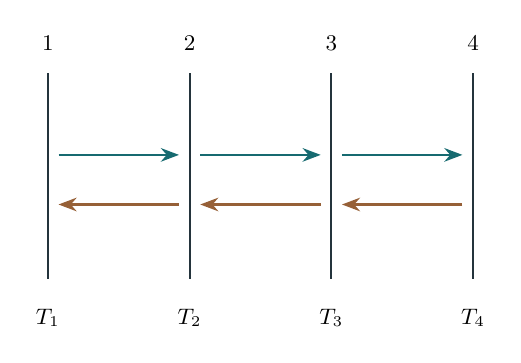
\begin{tikzpicture}[scale=.9,transform shape]
\draw[object] (0.00000,-1.30000)--(0.00000,1.60000);\node[above] at (0.00000,1.80000) {1};\node[below] at (0.00000,-1.60000) {$T_1$};\draw[motion] (0.15000,0.45000)--(1.85000,0.45000);\draw[force] (1.85000,-0.25000)--(0.15000,-0.25000);\draw[object] (2.00000,-1.30000)--(2.00000,1.60000);\node[above] at (2.00000,1.80000) {2};\node[below] at (2.00000,-1.60000) {$T_2$};\draw[motion] (2.15000,0.45000)--(3.85000,0.45000);\draw[force] (3.85000,-0.25000)--(2.15000,-0.25000);\draw[object] (4.00000,-1.30000)--(4.00000,1.60000);\node[above] at (4.00000,1.80000) {3};\node[below] at (4.00000,-1.60000) {$T_3$};\draw[motion] (4.15000,0.45000)--(5.85000,0.45000);\draw[force] (5.85000,-0.25000)--(4.15000,-0.25000);\draw[object] (6.00000,-1.30000)--(6.00000,1.60000);\node[above] at (6.00000,1.80000) {4};\node[below] at (6.00000,-1.60000) {$T_4$};
\end{tikzpicture}
\figcaption{图近1.4\quad 各间隙有相向辐射，中间板温度由平衡决定。}
\end{minipage}\end{center}

\Needspace{6\baselineskip}\subsection*{解答}


图近1.4从热端到冷端依次标板1、2、3、4。两端温度由外界维持，中间两板仅靠辐射交换达到稳态。先换成热力学温度，$T_1=373.15\,\mathrm K$、$T_4=283.15\,\mathrm K$，Stefan定律中的温度均用K。

每个黑表面向它面前的半空间发出$\sigma T^4$的能流密度。无限平行面的相互视角因子为1，一面的全部半空间辐射都到达相邻板。虽然单条光线可以斜射，角分布积分后的净能流沿法线。黑板不透光，板两侧分别与各自相邻的表面交换。因此相邻两板间沿热端到冷端的净流为
\[
q_{j,j+1}=\sigma(T_j^4-T_{j+1}^4).
\]
解图近1.4A画三条间隙中的净流；每条净流由相向的两份辐射相减得到。板内部导热使同一板的两面等温，支撑导热、边缘绕行和其他外部热交换按题设忽略。
\begin{center}\begin{minipage}{.98\linewidth}\centering
\begin{tikzpicture}[scale=.9,transform shape]
\draw[object] (0,-1.5)--(0,1.5);\node[above] at (0,1.6) {$T_1$};\node[below] at (0,-1.6) {板1};
\draw[force] (0.3,0)--(1.7,0) node[midway,above] {$q$};
\draw[object] (2,-1.5)--(2,1.5);\node[above] at (2,1.6) {$T_2$};\node[below] at (2,-1.6) {板2};
\draw[force] (2.3,0)--(3.7,0) node[midway,above] {$q$};
\draw[object] (4,-1.5)--(4,1.5);\node[above] at (4,1.6) {$T_3$};\node[below] at (4,-1.6) {板3};
\draw[force] (4.3,0)--(5.7,0) node[midway,above] {$q$};
\draw[object] (6,-1.5)--(6,1.5);\node[above] at (6,1.6) {$T_4$};\node[below] at (6,-1.6) {板4};
\node[left] at (-.5,.8) {热端};\node[right] at (6.5,.8) {冷端};
\end{tikzpicture}
\figcaption{解图近1.4A\quad 四板之间的三段稳态净辐射流相同}
\end{minipage}\end{center}
对中间板2，左面净吸收$\sigma(T_1^4-T_2^4)$，右面净吸收$\sigma(T_3^4-T_2^4)$。两面发射都使用板2的同一温度，稳态的单位面积能量守恒为
\[
 0=\sigma T_1^4+\sigma T_3^4-2\sigma T_2^4.
\]
板3同样吸收板2和板4的辐射，两面各发射$\sigma T_3^4$，所以
\[
T_1^4+T_3^4=2T_2^4,\qquad T_2^4+T_4^4=2T_3^4,
\]
解图近1.4B把一个内板的四项能量画开，两个发射项相加给系数2。若左、右净流暂时不同，其差改变板的内能，直到温度使两者相等。
\begin{center}\begin{minipage}{.98\linewidth}\centering
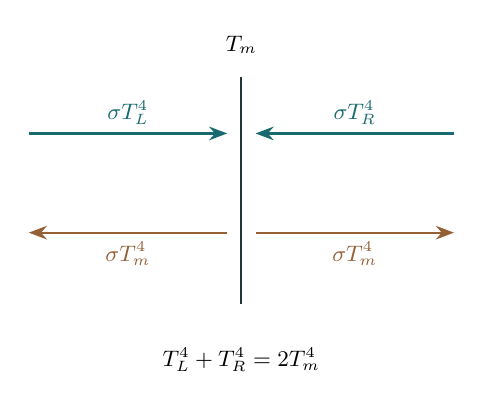
\begin{tikzpicture}[scale=.9,transform shape]
\draw[object] (0,-1.6)--(0,1.6);\node[above] at (0,1.8) {$T_m$};
\draw[motion] (-3,.8)--(-.2,.8) node[midway,above] {$\sigma T_L^4$};
\draw[force,color=warm] (-.2,-.6)--(-3,-.6) node[midway,below] {$\sigma T_m^4$};
\draw[motion] (3,.8)--(.2,.8) node[midway,above] {$\sigma T_R^4$};
\draw[force,color=warm] (.2,-.6)--(3,-.6) node[midway,below] {$\sigma T_m^4$};
\node[below] at (0,-2.1) {$T_L^4+T_R^4=2T_m^4$};
\end{tikzpicture}
\figcaption{解图近1.4B\quad 一个内板的两份吸收与两面发射}
\end{minipage}\end{center}
记$X_j=T_j^4$，上述方程成为$2X_2-X_3=X_1$、$-X_2+2X_3=X_4$。将第一式乘2再与第二式相加，得$3X_2=2X_1+X_4$；把$X_2$代回，得$3X_3=X_1+2X_4$。因此
\[
\boxed{T_2=\left(\frac{2T_1^4+T_4^4}{3}\right)^{1/4}=350.36\,\mathrm K},
\quad
\boxed{T_3=\left(\frac{T_1^4+2T_4^4}{3}\right)^{1/4}=321.98\,\mathrm K}.
\]
换回摄氏温度约为$77.21^\circ\mathrm C$和$48.83^\circ\mathrm C$。解图近1.4C取$T_h=T_1$、$T_c=T_4$，画$X_j$的等差排列，同时显示还原后的温度变化；四次方变量的等差关系直接给
\[
T_1^4-T_2^4=T_2^4-T_3^4=T_3^4-T_4^4
=\frac{T_1^4-T_4^4}{3}.
\]
\begin{center}\begin{minipage}{.98\linewidth}\centering
\begin{tikzpicture}[scale=.88,transform shape]
\draw[axis] (0,0.0)--(7.3,0.0) node[right] {$j$};
\draw[axis] (0,0)--(0,2.8);
\node[above left] at (0,2.8) {归一化量};
\draw[thin] (0.000000,0.0)--(0.000000,-0.06);\node[below,font=\scriptsize] at (0.000000,-0.08) {$ 1 $};
\draw[thin] (2.333333,0.0)--(2.333333,-0.06);\node[below,font=\scriptsize] at (2.333333,-0.08) {$ 2 $};
\draw[thin] (4.666667,0.0)--(4.666667,-0.06);\node[below,font=\scriptsize] at (4.666667,-0.08) {$ 3 $};
\draw[thin] (7.000000,0.0)--(7.000000,-0.06);\node[below,font=\scriptsize] at (7.000000,-0.08) {$ 4 $};
\draw[thin] (0,0.000000)--(-.06,0.000000);\node[left,font=\scriptsize] at (-.08,0.000000) {$ 0 $};
\draw[thin] (0,0.793651)--(-.06,0.793651);\node[left,font=\scriptsize] at (-.08,0.793651) {$ 0.333333 $};
\draw[thin] (0,1.587302)--(-.06,1.587302);\node[left,font=\scriptsize] at (-.08,1.587302) {$ 0.666667 $};
\draw[thin] (0,2.380952)--(-.06,2.380952);\node[left,font=\scriptsize] at (-.08,2.380952) {$ 1 $};
\draw[thick,color=accent] plot coordinates {(0.0000000,2.3809524) (0.0291667,2.3710317) (0.0583333,2.3611111) (0.0875000,2.3511905) (0.1166667,2.3412698) (0.1458333,2.3313492) (0.1750000,2.3214286) (0.2041667,2.3115079) (0.2333333,2.3015873) (0.2625000,2.2916667) (0.2916667,2.2817460) (0.3208333,2.2718254) (0.3500000,2.2619048) (0.3791667,2.2519841) (0.4083333,2.2420635) (0.4375000,2.2321429) (0.4666667,2.2222222) (0.4958333,2.2123016) (0.5250000,2.2023810) (0.5541667,2.1924603) (0.5833333,2.1825397) (0.6125000,2.1726190) (0.6416667,2.1626984) (0.6708333,2.1527778) (0.7000000,2.1428571) (0.7291667,2.1329365) (0.7583333,2.1230159) (0.7875000,2.1130952) (0.8166667,2.1031746) (0.8458333,2.0932540) (0.8750000,2.0833333) (0.9041667,2.0734127) (0.9333333,2.0634921) (0.9625000,2.0535714) (0.9916667,2.0436508) (1.0208333,2.0337302) (1.0500000,2.0238095) (1.0791667,2.0138889) (1.1083333,2.0039683) (1.1375000,1.9940476) (1.1666667,1.9841270) (1.1958333,1.9742063) (1.2250000,1.9642857) (1.2541667,1.9543651) (1.2833333,1.9444444) (1.3125000,1.9345238) (1.3416667,1.9246032) (1.3708333,1.9146825) (1.4000000,1.9047619) (1.4291667,1.8948413) (1.4583333,1.8849206) (1.4875000,1.8750000) (1.5166667,1.8650794) (1.5458333,1.8551587) (1.5750000,1.8452381) (1.6041667,1.8353175) (1.6333333,1.8253968) (1.6625000,1.8154762) (1.6916667,1.8055556) (1.7208333,1.7956349) (1.7500000,1.7857143) (1.7791667,1.7757937) (1.8083333,1.7658730) (1.8375000,1.7559524) (1.8666667,1.7460317) (1.8958333,1.7361111) (1.9250000,1.7261905) (1.9541667,1.7162698) (1.9833333,1.7063492) (2.0125000,1.6964286) (2.0416667,1.6865079) (2.0708333,1.6765873) (2.1000000,1.6666667) (2.1291667,1.6567460) (2.1583333,1.6468254) (2.1875000,1.6369048) (2.2166667,1.6269841) (2.2458333,1.6170635) (2.2750000,1.6071429) (2.3041667,1.5972222) (2.3333333,1.5873016) (2.3625000,1.5773810) (2.3916667,1.5674603) (2.4208333,1.5575397) (2.4500000,1.5476190) (2.4791667,1.5376984) (2.5083333,1.5277778) (2.5375000,1.5178571) (2.5666667,1.5079365) (2.5958333,1.4980159) (2.6250000,1.4880952) (2.6541667,1.4781746) (2.6833333,1.4682540) (2.7125000,1.4583333) (2.7416667,1.4484127) (2.7708333,1.4384921) (2.8000000,1.4285714) (2.8291667,1.4186508) (2.8583333,1.4087302) (2.8875000,1.3988095) (2.9166667,1.3888889) (2.9458333,1.3789683) (2.9750000,1.3690476) (3.0041667,1.3591270) (3.0333333,1.3492063) (3.0625000,1.3392857) (3.0916667,1.3293651) (3.1208333,1.3194444) (3.1500000,1.3095238) (3.1791667,1.2996032) (3.2083333,1.2896825) (3.2375000,1.2797619) (3.2666667,1.2698413) (3.2958333,1.2599206) (3.3250000,1.2500000) (3.3541667,1.2400794) (3.3833333,1.2301587) (3.4125000,1.2202381) (3.4416667,1.2103175) (3.4708333,1.2003968) (3.5000000,1.1904762) (3.5291667,1.1805556) (3.5583333,1.1706349) (3.5875000,1.1607143) (3.6166667,1.1507937) (3.6458333,1.1408730) (3.6750000,1.1309524) (3.7041667,1.1210317) (3.7333333,1.1111111) (3.7625000,1.1011905) (3.7916667,1.0912698) (3.8208333,1.0813492) (3.8500000,1.0714286) (3.8791667,1.0615079) (3.9083333,1.0515873) (3.9375000,1.0416667) (3.9666667,1.0317460) (3.9958333,1.0218254) (4.0250000,1.0119048) (4.0541667,1.0019841) (4.0833333,0.9920635) (4.1125000,0.9821429) (4.1416667,0.9722222) (4.1708333,0.9623016) (4.2000000,0.9523810) (4.2291667,0.9424603) (4.2583333,0.9325397) (4.2875000,0.9226190) (4.3166667,0.9126984) (4.3458333,0.9027778) (4.3750000,0.8928571) (4.4041667,0.8829365) (4.4333333,0.8730159) (4.4625000,0.8630952) (4.4916667,0.8531746) (4.5208333,0.8432540) (4.5500000,0.8333333) (4.5791667,0.8234127) (4.6083333,0.8134921) (4.6375000,0.8035714) (4.6666667,0.7936508) (4.6958333,0.7837302) (4.7250000,0.7738095) (4.7541667,0.7638889) (4.7833333,0.7539683) (4.8125000,0.7440476) (4.8416667,0.7341270) (4.8708333,0.7242063) (4.9000000,0.7142857) (4.9291667,0.7043651) (4.9583333,0.6944444) (4.9875000,0.6845238) (5.0166667,0.6746032) (5.0458333,0.6646825) (5.0750000,0.6547619) (5.1041667,0.6448413) (5.1333333,0.6349206) (5.1625000,0.6250000) (5.1916667,0.6150794) (5.2208333,0.6051587) (5.2500000,0.5952381) (5.2791667,0.5853175) (5.3083333,0.5753968) (5.3375000,0.5654762) (5.3666667,0.5555556) (5.3958333,0.5456349) (5.4250000,0.5357143) (5.4541667,0.5257937) (5.4833333,0.5158730) (5.5125000,0.5059524) (5.5416667,0.4960317) (5.5708333,0.4861111) (5.6000000,0.4761905) (5.6291667,0.4662698) (5.6583333,0.4563492) (5.6875000,0.4464286) (5.7166667,0.4365079) (5.7458333,0.4265873) (5.7750000,0.4166667) (5.8041667,0.4067460) (5.8333333,0.3968254) (5.8625000,0.3869048) (5.8916667,0.3769841) (5.9208333,0.3670635) (5.9500000,0.3571429) (5.9791667,0.3472222) (6.0083333,0.3373016) (6.0375000,0.3273810) (6.0666667,0.3174603) (6.0958333,0.3075397) (6.1250000,0.2976190) (6.1541667,0.2876984) (6.1833333,0.2777778) (6.2125000,0.2678571) (6.2416667,0.2579365) (6.2708333,0.2480159) (6.3000000,0.2380952) (6.3291667,0.2281746) (6.3583333,0.2182540) (6.3875000,0.2083333) (6.4166667,0.1984127) (6.4458333,0.1884921) (6.4750000,0.1785714) (6.5041667,0.1686508) (6.5333333,0.1587302) (6.5625000,0.1488095) (6.5916667,0.1388889) (6.6208333,0.1289683) (6.6500000,0.1190476) (6.6791667,0.1091270) (6.7083333,0.0992063) (6.7375000,0.0892857) (6.7666667,0.0793651) (6.7958333,0.0694444) (6.8250000,0.0595238) (6.8541667,0.0496032) (6.8833333,0.0396825) (6.9125000,0.0297619) (6.9416667,0.0198413) (6.9708333,0.0099206) (7.0000000,0.0000000)};
\draw[thick,color=accent] (7.65,2.55)--(8.15,2.55);\node[right,font=\scriptsize] at (8.2,2.55) {$(T_j^4-T_c^4)/(T_h^4-T_c^4)$};
\draw[thick,dashed,color=warm] plot coordinates {(0.0000000,2.3809524) (0.0291667,2.3740714) (0.0583333,2.3671759) (0.0875000,2.3602660) (0.1166667,2.3533415) (0.1458333,2.3464024) (0.1750000,2.3394485) (0.2041667,2.3324799) (0.2333333,2.3254963) (0.2625000,2.3184979) (0.2916667,2.3114844) (0.3208333,2.3044559) (0.3500000,2.2974122) (0.3791667,2.2903532) (0.4083333,2.2832790) (0.4375000,2.2761893) (0.4666667,2.2690842) (0.4958333,2.2619635) (0.5250000,2.2548272) (0.5541667,2.2476751) (0.5833333,2.2405073) (0.6125000,2.2333236) (0.6416667,2.2261240) (0.6708333,2.2189083) (0.7000000,2.2116765) (0.7291667,2.2044285) (0.7583333,2.1971641) (0.7875000,2.1898835) (0.8166667,2.1825863) (0.8458333,2.1752726) (0.8750000,2.1679423) (0.9041667,2.1605952) (0.9333333,2.1532313) (0.9625000,2.1458505) (0.9916667,2.1384527) (1.0208333,2.1310378) (1.0500000,2.1236057) (1.0791667,2.1161564) (1.1083333,2.1086897) (1.1375000,2.1012055) (1.1666667,2.0937038) (1.1958333,2.0861844) (1.2250000,2.0786472) (1.2541667,2.0710922) (1.2833333,2.0635193) (1.3125000,2.0559283) (1.3416667,2.0483191) (1.3708333,2.0406917) (1.4000000,2.0330460) (1.4291667,2.0253818) (1.4583333,2.0176990) (1.4875000,2.0099975) (1.5166667,2.0022773) (1.5458333,1.9945382) (1.5750000,1.9867801) (1.6041667,1.9790029) (1.6333333,1.9712065) (1.6625000,1.9633908) (1.6916667,1.9555557) (1.7208333,1.9477010) (1.7500000,1.9398266) (1.7791667,1.9319325) (1.8083333,1.9240184) (1.8375000,1.9160844) (1.8666667,1.9081303) (1.8958333,1.9001559) (1.9250000,1.8921611) (1.9541667,1.8841458) (1.9833333,1.8761100) (2.0125000,1.8680533) (2.0416667,1.8599759) (2.0708333,1.8518774) (2.1000000,1.8437579) (2.1291667,1.8356171) (2.1583333,1.8274549) (2.1875000,1.8192712) (2.2166667,1.8110658) (2.2458333,1.8028387) (2.2750000,1.7945897) (2.3041667,1.7863187) (2.3333333,1.7780255) (2.3625000,1.7697099) (2.3916667,1.7613719) (2.4208333,1.7530113) (2.4500000,1.7446279) (2.4791667,1.7362216) (2.5083333,1.7277923) (2.5375000,1.7193399) (2.5666667,1.7108640) (2.5958333,1.7023647) (2.6250000,1.6938418) (2.6541667,1.6852950) (2.6833333,1.6767244) (2.7125000,1.6681296) (2.7416667,1.6595105) (2.7708333,1.6508670) (2.8000000,1.6421989) (2.8291667,1.6335061) (2.8583333,1.6247884) (2.8875000,1.6160456) (2.9166667,1.6072775) (2.9458333,1.5984840) (2.9750000,1.5896649) (3.0041667,1.5808200) (3.0333333,1.5719492) (3.0625000,1.5630523) (3.0916667,1.5541290) (3.1208333,1.5451793) (3.1500000,1.5362029) (3.1791667,1.5271996) (3.2083333,1.5181693) (3.2375000,1.5091117) (3.2666667,1.5000268) (3.2958333,1.4909142) (3.3250000,1.4817737) (3.3541667,1.4726053) (3.3833333,1.4634086) (3.4125000,1.4541835) (3.4416667,1.4449298) (3.4708333,1.4356472) (3.5000000,1.4263356) (3.5291667,1.4169948) (3.5583333,1.4076244) (3.5875000,1.3982244) (3.6166667,1.3887944) (3.6458333,1.3793343) (3.6750000,1.3698438) (3.7041667,1.3603228) (3.7333333,1.3507709) (3.7625000,1.3411879) (3.7916667,1.3315737) (3.8208333,1.3219279) (3.8500000,1.3122504) (3.8791667,1.3025408) (3.9083333,1.2927989) (3.9375000,1.2830246) (3.9666667,1.2732174) (3.9958333,1.2633772) (4.0250000,1.2535038) (4.0541667,1.2435967) (4.0833333,1.2336559) (4.1125000,1.2236809) (4.1416667,1.2136716) (4.1708333,1.2036276) (4.2000000,1.1935487) (4.2291667,1.1834345) (4.2583333,1.1732849) (4.2875000,1.1630995) (4.3166667,1.1528780) (4.3458333,1.1426201) (4.3750000,1.1323255) (4.4041667,1.1219939) (4.4333333,1.1116249) (4.4625000,1.1012184) (4.4916667,1.0907739) (4.5208333,1.0802911) (4.5500000,1.0697697) (4.5791667,1.0592094) (4.6083333,1.0486098) (4.6375000,1.0379706) (4.6666667,1.0272914) (4.6958333,1.0165719) (4.7250000,1.0058117) (4.7541667,0.9950105) (4.7833333,0.9841679) (4.8125000,0.9732835) (4.8416667,0.9623569) (4.8708333,0.9513879) (4.9000000,0.9403759) (4.9291667,0.9293205) (4.9583333,0.9182215) (4.9875000,0.9070783) (5.0166667,0.8958906) (5.0458333,0.8846580) (5.0750000,0.8733799) (5.1041667,0.8620561) (5.1333333,0.8506860) (5.1625000,0.8392692) (5.1916667,0.8278053) (5.2208333,0.8162938) (5.2500000,0.8047343) (5.2791667,0.7931262) (5.3083333,0.7814691) (5.3375000,0.7697625) (5.3666667,0.7580060) (5.3958333,0.7461989) (5.4250000,0.7343409) (5.4541667,0.7224314) (5.4833333,0.7104698) (5.5125000,0.6984556) (5.5416667,0.6863884) (5.5708333,0.6742674) (5.6000000,0.6620923) (5.6291667,0.6498624) (5.6583333,0.6375771) (5.6875000,0.6252358) (5.7166667,0.6128380) (5.7458333,0.6003830) (5.7750000,0.5878702) (5.8041667,0.5752990) (5.8333333,0.5626688) (5.8625000,0.5499788) (5.8916667,0.5372285) (5.9208333,0.5244172) (5.9500000,0.5115441) (5.9791667,0.4986086) (6.0083333,0.4856099) (6.0375000,0.4725474) (6.0666667,0.4594203) (6.0958333,0.4462278) (6.1250000,0.4329693) (6.1541667,0.4196438) (6.1833333,0.4062506) (6.2125000,0.3927890) (6.2416667,0.3792580) (6.2708333,0.3656569) (6.3000000,0.3519848) (6.3291667,0.3382408) (6.3583333,0.3244240) (6.3875000,0.3105336) (6.4166667,0.2965685) (6.4458333,0.2825280) (6.4750000,0.2684109) (6.5041667,0.2542163) (6.5333333,0.2399433) (6.5625000,0.2255908) (6.5916667,0.2111577) (6.6208333,0.1966431) (6.6500000,0.1820457) (6.6791667,0.1673646) (6.7083333,0.1525985) (6.7375000,0.1377464) (6.7666667,0.1228069) (6.7958333,0.1077791) (6.8250000,0.0926615) (6.8541667,0.0774530) (6.8833333,0.0621522) (6.9125000,0.0467579) (6.9416667,0.0312687) (6.9708333,0.0156832) (7.0000000,0.0000000)};
\draw[thick,dashed,color=warm] (7.65,2.0999999999999996)--(8.15,2.0999999999999996);\node[right,font=\scriptsize] at (8.2,2.0999999999999996) {$(T_j-T_c)/(T_h-T_c)$};
\end{tikzpicture}
\figcaption{解图近1.4C\quad 四次方变量等差排列，温度还原后按非等差变化}
\end{minipage}\end{center}
每个间隙的净流均为$q=\sigma(T_1^4-T_4^4)/3$。不插中间板时，两端黑表面直接交换，$q_0=\sigma(T_1^4-T_4^4)$，故
\[
\boxed{q/q_0=1/3}.
\]
每个面本身仍按自己的$\sigma T_j^4$发射，增加中间板后，热端到冷端的总四次方温差分配在三个交换间隙中。各段净差变小，串联通过的稳态能流随之减小。

推广到插入$n$块等温黑板，两端编号为0与$n+1$，每块内板仍满足左右净流相等。相邻四次方温差共有$n+1$份，因而$q/q_0=1/(n+1)$，第$j$块内板有$T_j^4=T_h^4-j(T_h^4-T_c^4)/(n+1)$。解图近1.4D画插板数量对传热比的影响，单块给二分之一，两块给三分之一。在当前远场、足够大的平行板之间，相邻表面的视角因子均为1，因此净交换由相邻表面温度确定，改变间隙宽度仍得到上述稳态关系。
\begin{center}\begin{minipage}{.98\linewidth}\centering
\begin{tikzpicture}[scale=.88,transform shape]
\draw[axis] (0,0.0)--(7.3,0.0) node[right] {$n$};
\draw[axis] (0,0)--(0,2.8);
\node[above left] at (0,2.8) {$q/q_0$};
\draw[thin] (0.000000,0.0)--(0.000000,-0.06);\node[below,font=\scriptsize] at (0.000000,-0.08) {$ 0 $};
\draw[thin] (0.700000,0.0)--(0.700000,-0.06);\node[below,font=\scriptsize] at (0.700000,-0.08) {$ 1 $};
\draw[thin] (1.400000,0.0)--(1.400000,-0.06);\node[below,font=\scriptsize] at (1.400000,-0.08) {$ 2 $};
\draw[thin] (3.500000,0.0)--(3.500000,-0.06);\node[below,font=\scriptsize] at (3.500000,-0.08) {$ 5 $};
\draw[thin] (7.000000,0.0)--(7.000000,-0.06);\node[below,font=\scriptsize] at (7.000000,-0.08) {$ 10 $};
\draw[thin] (0,0.000000)--(-.06,0.000000);\node[left,font=\scriptsize] at (-.08,0.000000) {$ 0 $};
\draw[thin] (0,0.793651)--(-.06,0.793651);\node[left,font=\scriptsize] at (-.08,0.793651) {$ 0.333333 $};
\draw[thin] (0,1.190476)--(-.06,1.190476);\node[left,font=\scriptsize] at (-.08,1.190476) {$ 0.5 $};
\draw[thin] (0,2.380952)--(-.06,2.380952);\node[left,font=\scriptsize] at (-.08,2.380952) {$ 1 $};
\draw[thick,color=accent] plot coordinates {(0.0000000,2.3809524) (0.0291667,2.2857143) (0.0583333,2.1978022) (0.0875000,2.1164021) (0.1166667,2.0408163) (0.1458333,1.9704433) (0.1750000,1.9047619) (0.2041667,1.8433180) (0.2333333,1.7857143) (0.2625000,1.7316017) (0.2916667,1.6806723) (0.3208333,1.6326531) (0.3500000,1.5873016) (0.3791667,1.5444015) (0.4083333,1.5037594) (0.4375000,1.4652015) (0.4666667,1.4285714) (0.4958333,1.3937282) (0.5250000,1.3605442) (0.5541667,1.3289037) (0.5833333,1.2987013) (0.6125000,1.2698413) (0.6416667,1.2422360) (0.6708333,1.2158055) (0.7000000,1.1904762) (0.7291667,1.1661808) (0.7583333,1.1428571) (0.7875000,1.1204482) (0.8166667,1.0989011) (0.8458333,1.0781671) (0.8750000,1.0582011) (0.9041667,1.0389610) (0.9333333,1.0204082) (0.9625000,1.0025063) (0.9916667,0.9852217) (1.0208333,0.9685230) (1.0500000,0.9523810) (1.0791667,0.9367681) (1.1083333,0.9216590) (1.1375000,0.9070295) (1.1666667,0.8928571) (1.1958333,0.8791209) (1.2250000,0.8658009) (1.2541667,0.8528785) (1.2833333,0.8403361) (1.3125000,0.8281573) (1.3416667,0.8163265) (1.3708333,0.8048290) (1.4000000,0.7936508) (1.4291667,0.7827789) (1.4583333,0.7722008) (1.4875000,0.7619048) (1.5166667,0.7518797) (1.5458333,0.7421150) (1.5750000,0.7326007) (1.6041667,0.7233273) (1.6333333,0.7142857) (1.6625000,0.7054674) (1.6916667,0.6968641) (1.7208333,0.6884682) (1.7500000,0.6802721) (1.7791667,0.6722689) (1.8083333,0.6644518) (1.8375000,0.6568144) (1.8666667,0.6493506) (1.8958333,0.6420546) (1.9250000,0.6349206) (1.9541667,0.6279435) (1.9833333,0.6211180) (2.0125000,0.6144393) (2.0416667,0.6079027) (2.0708333,0.6015038) (2.1000000,0.5952381) (2.1291667,0.5891016) (2.1583333,0.5830904) (2.1875000,0.5772006) (2.2166667,0.5714286) (2.2458333,0.5657709) (2.2750000,0.5602241) (2.3041667,0.5547850) (2.3333333,0.5494505) (2.3625000,0.5442177) (2.3916667,0.5390836) (2.4208333,0.5340454) (2.4500000,0.5291005) (2.4791667,0.5242464) (2.5083333,0.5194805) (2.5375000,0.5148005) (2.5666667,0.5102041) (2.5958333,0.5056890) (2.6250000,0.5012531) (2.6541667,0.4968944) (2.6833333,0.4926108) (2.7125000,0.4884005) (2.7416667,0.4842615) (2.7708333,0.4801921) (2.8000000,0.4761905) (2.8291667,0.4722550) (2.8583333,0.4683841) (2.8875000,0.4645761) (2.9166667,0.4608295) (2.9458333,0.4571429) (2.9750000,0.4535147) (3.0041667,0.4499438) (3.0333333,0.4464286) (3.0625000,0.4429679) (3.0916667,0.4395604) (3.1208333,0.4362050) (3.1500000,0.4329004) (3.1791667,0.4296455) (3.2083333,0.4264392) (3.2375000,0.4232804) (3.2666667,0.4201681) (3.2958333,0.4171011) (3.3250000,0.4140787) (3.3541667,0.4110997) (3.3833333,0.4081633) (3.4125000,0.4052685) (3.4416667,0.4024145) (3.4708333,0.3996004) (3.5000000,0.3968254) (3.5291667,0.3940887) (3.5583333,0.3913894) (3.5875000,0.3887269) (3.6166667,0.3861004) (3.6458333,0.3835091) (3.6750000,0.3809524) (3.7041667,0.3784295) (3.7333333,0.3759398) (3.7625000,0.3734827) (3.7916667,0.3710575) (3.8208333,0.3686636) (3.8500000,0.3663004) (3.8791667,0.3639672) (3.9083333,0.3616637) (3.9375000,0.3593890) (3.9666667,0.3571429) (3.9958333,0.3549246) (4.0250000,0.3527337) (4.0541667,0.3505697) (4.0833333,0.3484321) (4.1125000,0.3463203) (4.1416667,0.3442341) (4.1708333,0.3421728) (4.2000000,0.3401361) (4.2291667,0.3381234) (4.2583333,0.3361345) (4.2875000,0.3341688) (4.3166667,0.3322259) (4.3458333,0.3303055) (4.3750000,0.3284072) (4.4041667,0.3265306) (4.4333333,0.3246753) (4.4625000,0.3228410) (4.4916667,0.3210273) (4.5208333,0.3192338) (4.5500000,0.3174603) (4.5791667,0.3157064) (4.6083333,0.3139717) (4.6375000,0.3122560) (4.6666667,0.3105590) (4.6958333,0.3088803) (4.7250000,0.3072197) (4.7541667,0.3055768) (4.7833333,0.3039514) (4.8125000,0.3023432) (4.8416667,0.3007519) (4.8708333,0.2991773) (4.9000000,0.2976190) (4.9291667,0.2960770) (4.9583333,0.2945508) (4.9875000,0.2930403) (5.0166667,0.2915452) (5.0458333,0.2900653) (5.0750000,0.2886003) (5.1041667,0.2871500) (5.1333333,0.2857143) (5.1625000,0.2842928) (5.1916667,0.2828854) (5.2208333,0.2814919) (5.2500000,0.2801120) (5.2791667,0.2787456) (5.3083333,0.2773925) (5.3375000,0.2760524) (5.3666667,0.2747253) (5.3958333,0.2734108) (5.4250000,0.2721088) (5.4541667,0.2708192) (5.4833333,0.2695418) (5.5125000,0.2682763) (5.5416667,0.2670227) (5.5708333,0.2657807) (5.6000000,0.2645503) (5.6291667,0.2633311) (5.6583333,0.2621232) (5.6875000,0.2609263) (5.7166667,0.2597403) (5.7458333,0.2585650) (5.7750000,0.2574003) (5.8041667,0.2562460) (5.8333333,0.2551020) (5.8625000,0.2539683) (5.8916667,0.2528445) (5.9208333,0.2517306) (5.9500000,0.2506266) (5.9791667,0.2495321) (6.0083333,0.2484472) (6.0375000,0.2473717) (6.0666667,0.2463054) (6.0958333,0.2452483) (6.1250000,0.2442002) (6.1541667,0.2431611) (6.1833333,0.2421308) (6.2125000,0.2411091) (6.2416667,0.2400960) (6.2708333,0.2390915) (6.3000000,0.2380952) (6.3291667,0.2371073) (6.3583333,0.2361275) (6.3875000,0.2351558) (6.4166667,0.2341920) (6.4458333,0.2332362) (6.4750000,0.2322880) (6.5041667,0.2313476) (6.5333333,0.2304147) (6.5625000,0.2294894) (6.5916667,0.2285714) (6.6208333,0.2276608) (6.6500000,0.2267574) (6.6791667,0.2258611) (6.7083333,0.2249719) (6.7375000,0.2240896) (6.7666667,0.2232143) (6.7958333,0.2223457) (6.8250000,0.2214839) (6.8541667,0.2206288) (6.8833333,0.2197802) (6.9125000,0.2189381) (6.9416667,0.2181025) (6.9708333,0.2172732) (7.0000000,0.2164502)};
\end{tikzpicture}
\figcaption{解图近1.4D\quad $n$块黑屏形成$n+1$个交换间隙，图线在整数$n$处给相应传热比}
\end{minipage}\end{center}


\Needspace{13\baselineskip}

\pdfbookmark[2]{第 5 题 真空包层下液氦的蒸发}{q5}

\section*{第 5 题\quad 真空包层下液氦的蒸发}\label{q:5}

黑色圆筒形容器直径$d=5.0\,\mathrm{cm}$、高$l=10.0\,\mathrm{cm}$，内盛沸点4.2K的液氦，汽化潜热$L_v=2.1\times10^4\,\mathrm{J/kg}$。侧壁及底部外包77K的绝热层，中间窄隙抽成真空。外包层在所涉及波段按漫灰体近似，发射率$\varepsilon=1/2$；两相对表面积近似相等。忽略开口、支撑、气体导热及其他热交换，汽化氦气立即逸出。取$\sigma=5.67\times10^{-8}\,\mathrm{W/(m^2K^4)}$，求每小时蒸发液氦质量。

\begin{center}\begin{minipage}{.98\linewidth}\centering
\begin{tikzpicture}[scale=.9,transform shape]
\draw[object] (0.00000,1.50000)--(0.00000,-1.50000)--(3.00000,-1.50000)--(3.00000,1.50000);\draw[object] (-0.35000,1.50000)--(-0.35000,-1.85000)--(3.35000,-1.85000)--(3.35000,1.50000);\node[above] at (1.50000,0.00000) {液氦 4.2K};\node[right] at (4.00000,0.00000) {包层77K};\node[right] at (4.00000,-0.70000) {窄真空间隙};\draw[<->,thin,color=muted] (0.00000,-2.40000)--(3.00000,-2.40000);\node[below] at (1.50000,-2.40000) {$d$};\draw[<->,thin,color=muted] (-1.00000,-1.50000)--(-1.00000,1.50000);\node[left] at (-1.00000,0.00000) {$l$};
\end{tikzpicture}
\figcaption{图近1.5\quad 侧壁和底面参与窄隙辐射交换，开口另行忽略。}
\end{minipage}\end{center}

\Needspace{6\baselineskip}\subsection*{解答}


图近1.5中，液氦和黑色容器壁为冷端，$T_1=4.2\,\mathrm K$；液氮温度的外包层为热端，$T_2=77\,\mathrm K$。窄隙抽真空，气体和固体漏热按题设忽略，保留两表面间的辐射交换。外包层在涉及波段取漫灰体，发射率$\varepsilon=1/2$，同一灰体吸收率也取$\varepsilon$，余下$1-\varepsilon$作反射。

黑壁的总出射度为$J_1=\sigma T_1^4$，每平方米每秒向外发出的能量由此给出。窄隙两相对面的面积近似相同，彼此视角因子取1。外层射向冷壁的能量分为自身发射$\varepsilon\sigma T_2^4$和对冷壁辐射的反射$(1-\varepsilon)J_1$，因此
\[
J_2=\varepsilon\sigma T_2^4+(1-\varepsilon)J_1.
\]
冷壁吸收外层射来的全部能流$J_2$，同时失去自身发射$J_1$。两项相减，
\[
q_{\rm in}=J_2-J_1
=\varepsilon\sigma(T_2^4-T_1^4).
\]
解图近1.5A把这三项单独标出，灰层反射使黑壁发出的那一部分能量回到冷端。展开后冷壁的净损失只留下$\varepsilon\sigma T_1^4$，外层温度更高，净流指向液氦。
\begin{center}\begin{minipage}{.98\linewidth}\centering
\begin{tikzpicture}[scale=.9,transform shape]
\draw[object] (0,-1.7)--(0,1.8);\draw[object] (5,-1.7)--(5,1.8);
\node[above] at (0,2) {黑冷壁4.2K};\node[above] at (5,2) {灰外层77K};
\draw[motion] (.2,1.1)--(4.8,1.1) node[midway,above] {$J_1=\sigma T_1^4$};
\draw[force,color=warm] (4.8,.1)--(.2,.1) node[midway,above] {$\varepsilon\sigma T_2^4$};
\draw[force,color=muted] (4.8,-.9)--(.2,-.9) node[midway,above] {$(1-\varepsilon)J_1$};
\node[below] at (2.5,-2) {$q_{\rm in}=J_2-J_1$};
\end{tikzpicture}
\figcaption{解图近1.5A\quad 冷壁出射、灰层发射和反射回流共同给净吸热}
\end{minipage}\end{center}
参与交换的表面为圆筒侧壁和底部，顶部开口与其他热路按题设排除。解图近1.5B分别标$d,l$及两份面积。侧面积为周长乘高$\pi dl$，底面积为$\pi(d/2)^2$，所以
\[
A=\pi dl+\frac{\pi d^2}{4}
=\pi(0.050)(0.100)+\frac{\pi(0.050)^2}{4}
=1.7671\times10^{-2}\,\mathrm{m^2}.
\]
这里$d=0.050\,\mathrm m$、$l=0.100\,\mathrm m$，面积以平方米计。把能流密度乘该面积，再代$\sigma=5.67\times10^{-8}\,\mathrm{W/(m^2K^4)}$，
\[
\dot Q=\frac12\sigma A(77^4-4.2^4)
=1.7611\times10^{-2}\,\mathrm W.
\]
得到约17.61mW的持续热输入。$77^4=35153041$、$4.2^4=311.1696$，比值$(4.2/77)^4\simeq8.85\times10^{-6}$。解图近1.5C在同一交换模型下画热输入随外层温度的变化，冷端项完整保留，其当前数值较小。
\begin{center}\begin{minipage}{.98\linewidth}\centering
\begin{tikzpicture}[scale=.9,transform shape]
\draw[object] (0,0) ellipse[x radius=1.5,y radius=.35];
\draw[object] (-1.5,0)--(-1.5,-2.8);\draw[object] (1.5,0)--(1.5,-2.8);
\draw[object] (0,-2.8) ellipse[x radius=1.5,y radius=.35];
\draw[<->] (-1.5,.7)--(1.5,.7) node[midway,above] {$d$};
\draw[<->] (2,-.1)--(2,-2.8) node[midway,right] {$l$};
\node at (0,-1.3) {4.2K};
\node[right,align=left] at (3,-1.3) {侧面：$\pi dl$\\[6pt]底部：$\pi d^2/4$\\[6pt]顶部开口};
\end{tikzpicture}
\figcaption{解图近1.5B\quad 辐射交换面积包括圆筒侧面与底部}
\end{minipage}\end{center}
\begin{center}\begin{minipage}{.98\linewidth}\centering
\begin{tikzpicture}[scale=.88,transform shape]
\draw[axis] (0,0.0)--(7.3,0.0) node[right] {$T_2/\mathrm K$};
\draw[axis] (0,0)--(0,2.8);
\node[above left] at (0,2.8) {$\dot Q/\mathrm{mW}$};
\draw[thin] (0.000000,0.0)--(0.000000,-0.06);\node[below,font=\scriptsize] at (0.000000,-0.08) {$ 10 $};
\draw[thin] (2.333333,0.0)--(2.333333,-0.06);\node[below,font=\scriptsize] at (2.333333,-0.08) {$ 40 $};
\draw[thin] (5.211111,0.0)--(5.211111,-0.06);\node[below,font=\scriptsize] at (5.211111,-0.08) {$ 77 $};
\draw[thin] (7.000000,0.0)--(7.000000,-0.06);\node[below,font=\scriptsize] at (7.000000,-0.08) {$ 100 $};
\draw[thin] (0,0.000000)--(-.06,0.000000);\node[left,font=\scriptsize] at (-.08,0.000000) {$ 0 $};
\draw[thin] (0,0.846683)--(-.06,0.846683);\node[left,font=\scriptsize] at (-.08,0.846683) {$ 17.611 $};
\draw[thin] (0,1.442308)--(-.06,1.442308);\node[left,font=\scriptsize] at (-.08,1.442308) {$ 30 $};
\draw[thin] (0,2.403846)--(-.06,2.403846);\node[left,font=\scriptsize] at (-.08,2.403846) {$ 50 $};
\draw[thick,color=accent] plot coordinates {(0.0000000,0.0002334) (0.0291667,0.0002716) (0.0583333,0.0003142) (0.0875000,0.0003615) (0.1166667,0.0004138) (0.1458333,0.0004715) (0.1750000,0.0005349) (0.2041667,0.0006044) (0.2333333,0.0006804) (0.2625000,0.0007633) (0.2916667,0.0008534) (0.3208333,0.0009513) (0.3500000,0.0010572) (0.3791667,0.0011717) (0.4083333,0.0012952) (0.4375000,0.0014281) (0.4666667,0.0015710) (0.4958333,0.0017243) (0.5250000,0.0018884) (0.5541667,0.0020640) (0.5833333,0.0022515) (0.6125000,0.0024514) (0.6416667,0.0026644) (0.6708333,0.0028908) (0.7000000,0.0031314) (0.7291667,0.0033866) (0.7583333,0.0036571) (0.7875000,0.0039435) (0.8166667,0.0042463) (0.8458333,0.0045662) (0.8750000,0.0049038) (0.9041667,0.0052598) (0.9333333,0.0056348) (0.9625000,0.0060294) (0.9916667,0.0064444) (1.0208333,0.0068804) (1.0500000,0.0073382) (1.0791667,0.0078184) (1.1083333,0.0083218) (1.1375000,0.0088491) (1.1666667,0.0094010) (1.1958333,0.0099784) (1.2250000,0.0105819) (1.2541667,0.0112124) (1.2833333,0.0118706) (1.3125000,0.0125573) (1.3416667,0.0132734) (1.3708333,0.0140197) (1.4000000,0.0147970) (1.4291667,0.0156062) (1.4583333,0.0164481) (1.4875000,0.0173236) (1.5166667,0.0182336) (1.5458333,0.0191789) (1.5750000,0.0201605) (1.6041667,0.0211794) (1.6333333,0.0222363) (1.6625000,0.0233323) (1.6916667,0.0244683) (1.7208333,0.0256453) (1.7500000,0.0268642) (1.7791667,0.0281261) (1.8083333,0.0294319) (1.8375000,0.0307826) (1.8666667,0.0321793) (1.8958333,0.0336230) (1.9250000,0.0351147) (1.9541667,0.0366555) (1.9833333,0.0382464) (2.0125000,0.0398885) (2.0416667,0.0415830) (2.0708333,0.0433309) (2.1000000,0.0451333) (2.1291667,0.0469913) (2.1583333,0.0489061) (2.1875000,0.0508789) (2.2166667,0.0529107) (2.2458333,0.0550028) (2.2750000,0.0571563) (2.3041667,0.0593724) (2.3333333,0.0616523) (2.3625000,0.0639973) (2.3916667,0.0664085) (2.4208333,0.0688872) (2.4500000,0.0714347) (2.4791667,0.0740521) (2.5083333,0.0767408) (2.5375000,0.0795021) (2.5666667,0.0823373) (2.5958333,0.0852475) (2.6250000,0.0882343) (2.6541667,0.0912989) (2.6833333,0.0944426) (2.7125000,0.0976667) (2.7416667,0.1009728) (2.7708333,0.1043620) (2.8000000,0.1078359) (2.8291667,0.1113957) (2.8583333,0.1150430) (2.8875000,0.1187791) (2.9166667,0.1226055) (2.9458333,0.1265236) (2.9750000,0.1305348) (3.0041667,0.1346407) (3.0333333,0.1388427) (3.0625000,0.1431422) (3.0916667,0.1475409) (3.1208333,0.1520401) (3.1500000,0.1566415) (3.1791667,0.1613465) (3.2083333,0.1661568) (3.2375000,0.1710737) (3.2666667,0.1760991) (3.2958333,0.1812343) (3.3250000,0.1864810) (3.3541667,0.1918408) (3.3833333,0.1973153) (3.4125000,0.2029062) (3.4416667,0.2086150) (3.4708333,0.2144434) (3.5000000,0.2203932) (3.5291667,0.2264658) (3.5583333,0.2326632) (3.5875000,0.2389868) (3.6166667,0.2454385) (3.6458333,0.2520199) (3.6750000,0.2587328) (3.7041667,0.2655789) (3.7333333,0.2725600) (3.7625000,0.2796778) (3.7916667,0.2869342) (3.8208333,0.2943308) (3.8500000,0.3018695) (3.8791667,0.3095521) (3.9083333,0.3173804) (3.9375000,0.3253562) (3.9666667,0.3334815) (3.9958333,0.3417579) (4.0250000,0.3501875) (4.0541667,0.3587721) (4.0833333,0.3675135) (4.1125000,0.3764137) (4.1416667,0.3854746) (4.1708333,0.3946981) (4.2000000,0.4040862) (4.2291667,0.4136407) (4.2583333,0.4233636) (4.2875000,0.4332570) (4.3166667,0.4433227) (4.3458333,0.4535628) (4.3750000,0.4639793) (4.4041667,0.4745742) (4.4333333,0.4853496) (4.4625000,0.4963073) (4.4916667,0.5074496) (4.5208333,0.5187784) (4.5500000,0.5302959) (4.5791667,0.5420041) (4.6083333,0.5539051) (4.6375000,0.5660010) (4.6666667,0.5782940) (4.6958333,0.5907861) (4.7250000,0.6034795) (4.7541667,0.6163763) (4.7833333,0.6294788) (4.8125000,0.6427891) (4.8416667,0.6563093) (4.8708333,0.6700417) (4.9000000,0.6839885) (4.9291667,0.6981519) (4.9583333,0.7125341) (4.9875000,0.7271374) (5.0166667,0.7419640) (5.0458333,0.7570162) (5.0750000,0.7722963) (5.1041667,0.7878065) (5.1333333,0.8035492) (5.1625000,0.8195266) (5.1916667,0.8357411) (5.2208333,0.8521951) (5.2500000,0.8688908) (5.2791667,0.8858306) (5.3083333,0.9030170) (5.3375000,0.9204522) (5.3666667,0.9381386) (5.3958333,0.9560788) (5.4250000,0.9742750) (5.4541667,0.9927297) (5.4833333,1.0114454) (5.5125000,1.0304244) (5.5416667,1.0496693) (5.5708333,1.0691825) (5.6000000,1.0889666) (5.6291667,1.1090239) (5.6583333,1.1293570) (5.6875000,1.1499685) (5.7166667,1.1708608) (5.7458333,1.1920364) (5.7750000,1.2134981) (5.8041667,1.2352482) (5.8333333,1.2572894) (5.8625000,1.2796242) (5.8916667,1.3022553) (5.9208333,1.3251853) (5.9500000,1.3484168) (5.9791667,1.3719523) (6.0083333,1.3957947) (6.0375000,1.4199464) (6.0666667,1.4444103) (6.0958333,1.4691888) (6.1250000,1.4942849) (6.1541667,1.5197010) (6.1833333,1.5454401) (6.2125000,1.5715046) (6.2416667,1.5978976) (6.2708333,1.6246215) (6.3000000,1.6516793) (6.3291667,1.6790737) (6.3583333,1.7068074) (6.3875000,1.7348833) (6.4166667,1.7633041) (6.4458333,1.7920727) (6.4750000,1.8211919) (6.5041667,1.8506645) (6.5333333,1.8804934) (6.5625000,1.9106814) (6.5916667,1.9412315) (6.6208333,1.9721464) (6.6500000,2.0034292) (6.6791667,2.0350826) (6.7083333,2.0671096) (6.7375000,2.0995132) (6.7666667,2.1322962) (6.7958333,2.1654617) (6.8250000,2.1990126) (6.8541667,2.2329518) (6.8833333,2.2672824) (6.9125000,2.3020073) (6.9416667,2.3371296) (6.9708333,2.3726523) (7.0000000,2.4085783)};
\end{tikzpicture}
\figcaption{解图近1.5C\quad 固定4.2K冷壁时外层温度的四次方控制热输入}
\end{minipage}\end{center}
氦处于沸点，汽化气体立即离开，壁与液体维持$4.2\,\mathrm K$，输入热量转成汽化潜热。令$\dot m$为质量损失率，能量方程为$L_v\dot m=\dot Q$。一小时为3600s，因而
\[
\boxed{\Delta m=\frac{\dot Q(3600\,\mathrm s)}{L_v}
=3.02\times10^{-3}\,\mathrm{kg}\simeq3.0\,\mathrm g}.
\]
汽化潜热使用$L_v=2.1\times10^4\,\mathrm{J/kg}$，相应$\dot m$的单位为kg/s。将质量率乘以一小时的时间，得到约3克的液氦损失。

灰体条件使同一个$\varepsilon$同时用于77K发射与对4.2K入射谱的吸收。一般的总发射率是以自身温度辐射谱加权的平均量；取消灰体近似时，按每个频率的发射率与同频吸收率列式，再积分两种温度谱。对本题当前数值，冷端的四次方比给出这项修正的量级，而灰体表达式保持完整能量关系。

窄隙的近等面积近似也决定了交换系数。设黑冷壁面积为$A_1$、封闭灰外壳为$A_2$，冷壁完全看见外壳，记$a=A_1/A_2$。视角互易给外壳看见冷壁的比例$a$，外壳其余比例$1-a$看见自身。于是外层接收辐射为$G_2=aJ_1+(1-a)J_2$，并满足
\[
 J_2=\varepsilon\sigma T_2^4+(1-\varepsilon)
 [aJ_1+(1-a)J_2].
\]
把含$J_2$的项移到同一边，系数为$\varepsilon+a(1-\varepsilon)$，再求冷壁净流$A_1(J_2-J_1)$，得到
\[
\dot Q=\frac{A_1\sigma(T_2^4-T_1^4)}
{1+(A_1/A_2)(1/\varepsilon-1)}.
\]
记$\varepsilon_{\rm eff}=\dot Q/[A_1\sigma(T_2^4-T_1^4)]$，解图近1.5D画固定$\varepsilon=1/2$时这一有效交换系数。$a\simeq1$给$\varepsilon=1/2$，回到本题窄隙式；外壳面积增大使$a$减小，灰外壳的自视反射增加腔内辐射，系数向1增大。
\begin{center}\begin{minipage}{.98\linewidth}\centering
\begin{tikzpicture}[scale=.88,transform shape]
\draw[axis] (0,0.0)--(7.3,0.0) node[right] {$a=A_1/A_2$};
\draw[axis] (0,0)--(0,2.8);
\node[above left] at (0,2.8) {$\varepsilon_{\rm eff}$};
\draw[thin] (0.000000,0.0)--(0.000000,-0.06);\node[below,font=\scriptsize] at (0.000000,-0.08) {$ 0 $};
\draw[thin] (1.750000,0.0)--(1.750000,-0.06);\node[below,font=\scriptsize] at (1.750000,-0.08) {$ 0.25 $};
\draw[thin] (3.500000,0.0)--(3.500000,-0.06);\node[below,font=\scriptsize] at (3.500000,-0.08) {$ 0.5 $};
\draw[thin] (5.250000,0.0)--(5.250000,-0.06);\node[below,font=\scriptsize] at (5.250000,-0.08) {$ 0.75 $};
\draw[thin] (7.000000,0.0)--(7.000000,-0.06);\node[below,font=\scriptsize] at (7.000000,-0.08) {$ 1 $};
\draw[thin] (0,0.000000)--(-.06,0.000000);\node[left,font=\scriptsize] at (-.08,0.000000) {$ 0 $};
\draw[thin] (0,1.190476)--(-.06,1.190476);\node[left,font=\scriptsize] at (-.08,1.190476) {$ 0.5 $};
\draw[thin] (0,1.587302)--(-.06,1.587302);\node[left,font=\scriptsize] at (-.08,1.587302) {$ 0.666667 $};
\draw[thin] (0,2.380952)--(-.06,2.380952);\node[left,font=\scriptsize] at (-.08,2.380952) {$ 1 $};
\draw[thick,color=accent] plot coordinates {(0.0000000,2.3809524) (0.0291667,2.3710729) (0.0583333,2.3612751) (0.0875000,2.3515579) (0.1166667,2.3419204) (0.1458333,2.3323615) (0.1750000,2.3228804) (0.2041667,2.3134760) (0.2333333,2.3041475) (0.2625000,2.2948939) (0.2916667,2.2857143) (0.3208333,2.2766079) (0.3500000,2.2675737) (0.3791667,2.2586110) (0.4083333,2.2497188) (0.4375000,2.2408964) (0.4666667,2.2321429) (0.4958333,2.2234575) (0.5250000,2.2148394) (0.5541667,2.2062879) (0.5833333,2.1978022) (0.6125000,2.1893815) (0.6416667,2.1810251) (0.6708333,2.1727322) (0.7000000,2.1645022) (0.7291667,2.1563342) (0.7583333,2.1482277) (0.7875000,2.1401819) (0.8166667,2.1321962) (0.8458333,2.1242698) (0.8750000,2.1164021) (0.9041667,2.1085925) (0.9333333,2.1008403) (0.9625000,2.0931450) (0.9916667,2.0855057) (1.0208333,2.0779221) (1.0500000,2.0703934) (1.0791667,2.0629190) (1.1083333,2.0554985) (1.1375000,2.0481311) (1.1666667,2.0408163) (1.1958333,2.0335536) (1.2250000,2.0263425) (1.2541667,2.0191822) (1.2833333,2.0120724) (1.3125000,2.0050125) (1.3416667,1.9980020) (1.3708333,1.9910403) (1.4000000,1.9841270) (1.4291667,1.9772615) (1.4583333,1.9704433) (1.4875000,1.9636721) (1.5166667,1.9569472) (1.5458333,1.9502682) (1.5750000,1.9436346) (1.6041667,1.9370460) (1.6333333,1.9305019) (1.6625000,1.9240019) (1.6916667,1.9175455) (1.7208333,1.9111323) (1.7500000,1.9047619) (1.7791667,1.8984338) (1.8083333,1.8921476) (1.8375000,1.8859029) (1.8666667,1.8796992) (1.8958333,1.8735363) (1.9250000,1.8674136) (1.9541667,1.8613309) (1.9833333,1.8552876) (2.0125000,1.8492834) (2.0416667,1.8433180) (2.0708333,1.8373909) (2.1000000,1.8315018) (2.1291667,1.8256504) (2.1583333,1.8198362) (2.1875000,1.8140590) (2.2166667,1.8083183) (2.2458333,1.8026138) (2.2750000,1.7969452) (2.3041667,1.7913121) (2.3333333,1.7857143) (2.3625000,1.7801513) (2.3916667,1.7746229) (2.4208333,1.7691287) (2.4500000,1.7636684) (2.4791667,1.7582418) (2.5083333,1.7528484) (2.5375000,1.7474880) (2.5666667,1.7421603) (2.5958333,1.7368650) (2.6250000,1.7316017) (2.6541667,1.7263703) (2.6833333,1.7211704) (2.7125000,1.7160017) (2.7416667,1.7108640) (2.7708333,1.7057569) (2.8000000,1.7006803) (2.8291667,1.6956337) (2.8583333,1.6906171) (2.8875000,1.6856300) (2.9166667,1.6806723) (2.9458333,1.6757436) (2.9750000,1.6708438) (3.0041667,1.6659725) (3.0333333,1.6611296) (3.0625000,1.6563147) (3.0916667,1.6515277) (3.1208333,1.6467682) (3.1500000,1.6420361) (3.1791667,1.6373312) (3.2083333,1.6326531) (3.2375000,1.6280016) (3.2666667,1.6233766) (3.2958333,1.6187778) (3.3250000,1.6142050) (3.3541667,1.6096579) (3.3833333,1.6051364) (3.4125000,1.6006403) (3.4416667,1.5961692) (3.4708333,1.5917230) (3.5000000,1.5873016) (3.5291667,1.5829046) (3.5583333,1.5785320) (3.5875000,1.5741834) (3.6166667,1.5698587) (3.6458333,1.5655577) (3.6750000,1.5612802) (3.7041667,1.5570261) (3.7333333,1.5527950) (3.7625000,1.5485869) (3.7916667,1.5444015) (3.8208333,1.5402387) (3.8500000,1.5360983) (3.8791667,1.5319801) (3.9083333,1.5278839) (3.9375000,1.5238095) (3.9666667,1.5197568) (3.9958333,1.5157257) (4.0250000,1.5117158) (4.0541667,1.5077271) (4.0833333,1.5037594) (4.1125000,1.4998125) (4.1416667,1.4958863) (4.1708333,1.4919806) (4.2000000,1.4880952) (4.2291667,1.4842301) (4.2583333,1.4803849) (4.2875000,1.4765596) (4.3166667,1.4727541) (4.3458333,1.4689680) (4.3750000,1.4652015) (4.4041667,1.4614541) (4.4333333,1.4577259) (4.4625000,1.4540167) (4.4916667,1.4503263) (4.5208333,1.4466546) (4.5500000,1.4430014) (4.5791667,1.4393667) (4.6083333,1.4357502) (4.6375000,1.4321518) (4.6666667,1.4285714) (4.6958333,1.4250089) (4.7250000,1.4214641) (4.7541667,1.4179369) (4.7833333,1.4144272) (4.8125000,1.4109347) (4.8416667,1.4074595) (4.8708333,1.4040014) (4.9000000,1.4005602) (4.9291667,1.3971359) (4.9583333,1.3937282) (4.9875000,1.3903372) (5.0166667,1.3869626) (5.0458333,1.3836043) (5.0750000,1.3802622) (5.1041667,1.3769363) (5.1333333,1.3736264) (5.1625000,1.3703323) (5.1916667,1.3670540) (5.2208333,1.3637913) (5.2500000,1.3605442) (5.2791667,1.3573125) (5.3083333,1.3540961) (5.3375000,1.3508950) (5.3666667,1.3477089) (5.3958333,1.3445378) (5.4250000,1.3413816) (5.4541667,1.3382402) (5.4833333,1.3351135) (5.5125000,1.3320013) (5.5416667,1.3289037) (5.5708333,1.3258204) (5.6000000,1.3227513) (5.6291667,1.3196965) (5.6583333,1.3166557) (5.6875000,1.3136289) (5.7166667,1.3106160) (5.7458333,1.3076169) (5.7750000,1.3046314) (5.8041667,1.3016596) (5.8333333,1.2987013) (5.8625000,1.2957564) (5.8916667,1.2928248) (5.9208333,1.2899065) (5.9500000,1.2870013) (5.9791667,1.2841091) (6.0083333,1.2812300) (6.0375000,1.2783637) (6.0666667,1.2755102) (6.0958333,1.2726694) (6.1250000,1.2698413) (6.1541667,1.2670257) (6.1833333,1.2642225) (6.2125000,1.2614317) (6.2416667,1.2586532) (6.2708333,1.2558870) (6.3000000,1.2531328) (6.3291667,1.2503907) (6.3583333,1.2476606) (6.3875000,1.2449424) (6.4166667,1.2422360) (6.4458333,1.2395414) (6.4750000,1.2368584) (6.5041667,1.2341870) (6.5333333,1.2315271) (6.5625000,1.2288786) (6.5916667,1.2262416) (6.6208333,1.2236158) (6.6500000,1.2210012) (6.6791667,1.2183978) (6.7083333,1.2158055) (6.7375000,1.2132241) (6.7666667,1.2106538) (6.7958333,1.2080942) (6.8250000,1.2055455) (6.8541667,1.2030075) (6.8833333,1.2004802) (6.9125000,1.1979635) (6.9416667,1.1954573) (6.9708333,1.1929615) (7.0000000,1.1904762)};
\end{tikzpicture}
\figcaption{解图近1.5D\quad 发射率一半的灰外壳面积比改变腔内有效辐射交换}
\end{minipage}\end{center}


\Needspace{13\baselineskip}

\pdfbookmark[2]{第 6 题 黑体谱峰的温度标度}{q6}

\section*{第 6 题\quad 黑体谱峰的温度标度}\label{q:6}

由普朗克黑体辐射公式证明：按每单位真空波长定义的平衡辐射能量密度谱$u_\lambda(T)$，其峰值与绝对温度的五次方成正比。推导峰位置，并说明若按每单位频率定义谱，峰值的温度幂次是否相同。

\begin{center}\begin{minipage}{.98\linewidth}\centering
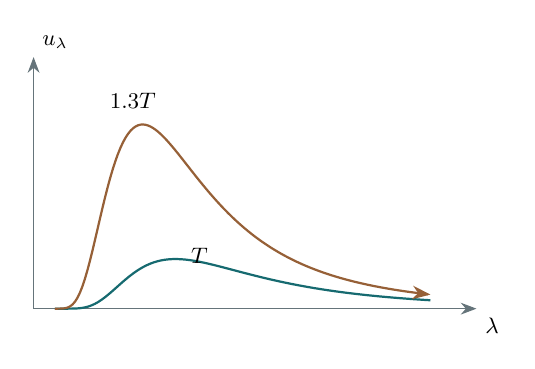
\begin{tikzpicture}[scale=.9,transform shape]
\draw[axis] (0.00000,0.00000)--(6.25000,0.00000);\draw[axis] (0.00000,0.00000)--(0.00000,3.55000);\node[below right] at (6.25000,0.00000) {$\lambda$};\node[above right] at (0.00000,3.55000) {$u_\lambda$};\draw[traj] plot coordinates {(0.30000,0.00000) (0.33557,0.00000) (0.37114,0.00000) (0.40671,0.00001) (0.44228,0.00003) (0.47785,0.00012) (0.51342,0.00036) (0.54899,0.00089) (0.58456,0.00196) (0.62013,0.00386) (0.65570,0.00696) (0.69128,0.01166) (0.72685,0.01832) (0.76242,0.02729) (0.79799,0.03883) (0.83356,0.05310) (0.86913,0.07016) (0.90470,0.08997) (0.94027,0.11238) (0.97584,0.13716) (1.01141,0.16403) (1.04698,0.19264) (1.08255,0.22261) (1.11812,0.25357) (1.15369,0.28512) (1.18926,0.31690) (1.22483,0.34855) (1.26040,0.37976) (1.29597,0.41023) (1.33154,0.43972) (1.36711,0.46800) (1.40268,0.49492) (1.43826,0.52031) (1.47383,0.54407) (1.50940,0.56613) (1.54497,0.58644) (1.58054,0.60496) (1.61611,0.62169) (1.65168,0.63665) (1.68725,0.64986) (1.72282,0.66138) (1.75839,0.67124) (1.79396,0.67952) (1.82953,0.68628) (1.86510,0.69160) (1.90067,0.69555) (1.93624,0.69821) (1.97181,0.69966) (2.00738,0.69998) (2.04295,0.69924) (2.07852,0.69753) (2.11409,0.69493) (2.14966,0.69149) (2.18523,0.68729) (2.22081,0.68240) (2.25638,0.67689) (2.29195,0.67081) (2.32752,0.66421) (2.36309,0.65716) (2.39866,0.64971) (2.43423,0.64190) (2.46980,0.63377) (2.50537,0.62537) (2.54094,0.61674) (2.57651,0.60791) (2.61208,0.59892) (2.64765,0.58979) (2.68322,0.58056) (2.71879,0.57125) (2.75436,0.56188) (2.78993,0.55247) (2.82550,0.54306) (2.86107,0.53364) (2.89664,0.52425) (2.93221,0.51489) (2.96779,0.50558) (3.00336,0.49633) (3.03893,0.48715) (3.07450,0.47805) (3.11007,0.46904) (3.14564,0.46013) (3.18121,0.45132) (3.21678,0.44263) (3.25235,0.43405) (3.28792,0.42558) (3.32349,0.41724) (3.35906,0.40903) (3.39463,0.40094) (3.43020,0.39299) (3.46577,0.38517) (3.50134,0.37748) (3.53691,0.36993) (3.57248,0.36251) (3.60805,0.35523) (3.64362,0.34808) (3.67919,0.34107) (3.71477,0.33419) (3.75034,0.32744) (3.78591,0.32083) (3.82148,0.31435) (3.85705,0.30800) (3.89262,0.30178) (3.92819,0.29568) (3.96376,0.28971) (3.99933,0.28387) (4.03490,0.27815) (4.07047,0.27254) (4.10604,0.26706) (4.14161,0.26169) (4.17718,0.25644) (4.21275,0.25130) (4.24832,0.24627) (4.28389,0.24135) (4.31946,0.23653) (4.35503,0.23182) (4.39060,0.22722) (4.42617,0.22271) (4.46174,0.21830) (4.49732,0.21399) (4.53289,0.20977) (4.56846,0.20565) (4.60403,0.20162) (4.63960,0.19767) (4.67517,0.19381) (4.71074,0.19004) (4.74631,0.18635) (4.78188,0.18274) (4.81745,0.17921) (4.85302,0.17576) (4.88859,0.17238) (4.92416,0.16908) (4.95973,0.16585) (4.99530,0.16269) (5.03087,0.15960) (5.06644,0.15658) (5.10201,0.15362) (5.13758,0.15073) (5.17315,0.14790) (5.20872,0.14514) (5.24430,0.14243) (5.27987,0.13978) (5.31544,0.13719) (5.35101,0.13466) (5.38658,0.13218) (5.42215,0.12975) (5.45772,0.12738) (5.49329,0.12506) (5.52886,0.12278) (5.56443,0.12056) (5.60000,0.11838)};\draw[force] plot coordinates {(0.30000,0.00001) (0.33557,0.00010) (0.37114,0.00052) (0.40671,0.00200) (0.44228,0.00595) (0.47785,0.01461) (0.51342,0.03089) (0.54899,0.05794) (0.58456,0.09870) (0.62013,0.15545) (0.65570,0.22944) (0.69128,0.32085) (0.72685,0.42875) (0.76242,0.55131) (0.79799,0.68603) (0.83356,0.82997) (0.86913,0.98000) (0.90470,1.13299) (0.94027,1.28599) (0.97584,1.43634) (1.01141,1.58171) (1.04698,1.72017) (1.08255,1.85019) (1.11812,1.97059) (1.15369,2.08055) (1.18926,2.17957) (1.22483,2.26741) (1.26040,2.34405) (1.29597,2.40967) (1.33154,2.46461) (1.36711,2.50928) (1.40268,2.54424) (1.43826,2.57005) (1.47383,2.58734) (1.50940,2.59675) (1.54497,2.59894) (1.58054,2.59453) (1.61611,2.58416) (1.65168,2.56843) (1.68725,2.54791) (1.72282,2.52314) (1.75839,2.49463) (1.79396,2.46286) (1.82953,2.42827) (1.86510,2.39126) (1.90067,2.35222) (1.93624,2.31147) (1.97181,2.26934) (2.00738,2.22609) (2.04295,2.18199) (2.07852,2.13727) (2.11409,2.09213) (2.14966,2.04674) (2.18523,2.00129) (2.22081,1.95590) (2.25638,1.91070) (2.29195,1.86581) (2.32752,1.82132) (2.36309,1.77732) (2.39866,1.73387) (2.43423,1.69105) (2.46980,1.64890) (2.50537,1.60746) (2.54094,1.56678) (2.57651,1.52688) (2.61208,1.48778) (2.64765,1.44950) (2.68322,1.41206) (2.71879,1.37546) (2.75436,1.33970) (2.78993,1.30480) (2.82550,1.27074) (2.86107,1.23753) (2.89664,1.20515) (2.93221,1.17360) (2.96779,1.14288) (3.00336,1.11295) (3.03893,1.08383) (3.07450,1.05548) (3.11007,1.02791) (3.14564,1.00108) (3.18121,0.97499) (3.21678,0.94963) (3.25235,0.92497) (3.28792,0.90100) (3.32349,0.87770) (3.35906,0.85505) (3.39463,0.83305) (3.43020,0.81167) (3.46577,0.79090) (3.50134,0.77071) (3.53691,0.75110) (3.57248,0.73205) (3.60805,0.71354) (3.64362,0.69556) (3.67919,0.67810) (3.71477,0.66113) (3.75034,0.64464) (3.78591,0.62862) (3.82148,0.61306) (3.85705,0.59794) (3.89262,0.58325) (3.92819,0.56898) (3.96376,0.55511) (3.99933,0.54163) (4.03490,0.52853) (4.07047,0.51580) (4.10604,0.50343) (4.14161,0.49140) (4.17718,0.47971) (4.21275,0.46835) (4.24832,0.45730) (4.28389,0.44656) (4.31946,0.43611) (4.35503,0.42596) (4.39060,0.41608) (4.42617,0.40647) (4.46174,0.39713) (4.49732,0.38804) (4.53289,0.37920) (4.56846,0.37059) (4.60403,0.36222) (4.63960,0.35407) (4.67517,0.34614) (4.71074,0.33843) (4.74631,0.33092) (4.78188,0.32360) (4.81745,0.31648) (4.85302,0.30955) (4.88859,0.30280) (4.92416,0.29623) (4.95973,0.28983) (4.99530,0.28359) (5.03087,0.27752) (5.06644,0.27160) (5.10201,0.26583) (5.13758,0.26021) (5.17315,0.25474) (5.20872,0.24940) (5.24430,0.24420) (5.27987,0.23913) (5.31544,0.23418) (5.35101,0.22936) (5.38658,0.22466) (5.42215,0.22008) (5.45772,0.21561) (5.49329,0.21125) (5.52886,0.20699) (5.56443,0.20284) (5.60000,0.19879)};\node[right] at (2.10000,0.75000) {$T$};\node[above] at (1.40000,2.70000) {$1.3T$};
\end{tikzpicture}
\figcaption{图近1.6\quad 同一波长坐标中的两温度普朗克谱。}
\end{minipage}\end{center}

\Needspace{6\baselineskip}\subsection*{解答}


题目按每单位真空波长定义谱密度$u_\lambda$，单位为$\mathrm{J/m^4}$；相应的$u_\nu$单位为$\mathrm{J/(m^3\,Hz)}$。图近1.6比较不同温度的波长谱，横轴为波长，纵轴给每单位波长区间的辐射能量密度。先从Planck频率谱出发，
\[
u_\nu(T)=\frac{8\pi h\nu^3}{c^3}\frac1{e^{h\nu/(k_BT)}-1}.
\]
同一小段辐射能量用两种变量表示时，满足$u_\lambda|\dd\lambda|=u_\nu|\dd\nu|$。由$\nu=c/\lambda$，$\dd\nu/\dd\lambda=-c/\lambda^2$，区间长度用其绝对值，故$u_\lambda=u_\nu(c/\lambda)\,c/\lambda^2$，得到
\[
u_\lambda(T)=\frac{8\pi hc}{\lambda^5}
\frac1{e^{hc/(\lambda k_BT)}-1}.
\]
这里$\nu^3$代换给$\lambda^{-3}$，区间换算再给$\lambda^{-2}$，两项共同形成$\lambda^{-5}$。解图近1.6A取参考温度$T_0$，记$b=\lambda_{\max}(T_0)T_0$作为横轴尺度，画温度增加后峰向短波移动、峰高增长的波长谱。下面由驻点条件求出$b$并说明它与温度无关。
\begin{center}\begin{minipage}{.98\linewidth}\centering
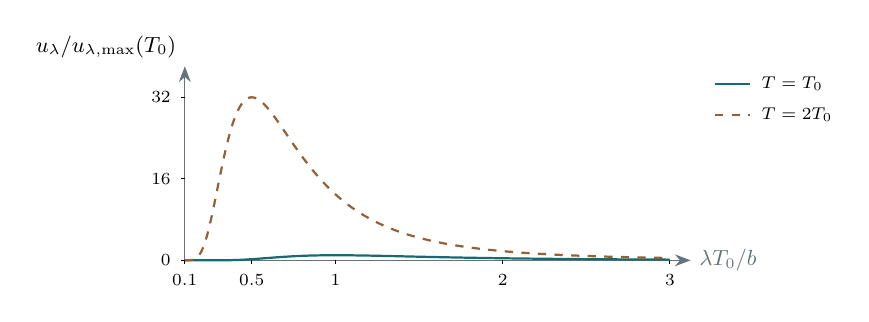
\begin{tikzpicture}[scale=.88,transform shape]
\draw[axis] (0,0.0)--(7.3,0.0) node[right] {$\lambda T_0/b$};
\draw[axis] (0,0)--(0,2.8);
\node[above left] at (0,2.8) {$u_\lambda/u_{\lambda,\max}(T_0)$};
\draw[thin] (0.000000,0.0)--(0.000000,-0.06);\node[below,font=\scriptsize] at (0.000000,-0.08) {$ 0.1 $};
\draw[thin] (0.965517,0.0)--(0.965517,-0.06);\node[below,font=\scriptsize] at (0.965517,-0.08) {$ 0.5 $};
\draw[thin] (2.172414,0.0)--(2.172414,-0.06);\node[below,font=\scriptsize] at (2.172414,-0.08) {$ 1 $};
\draw[thin] (4.586207,0.0)--(4.586207,-0.06);\node[below,font=\scriptsize] at (4.586207,-0.08) {$ 2 $};
\draw[thin] (7.000000,0.0)--(7.000000,-0.06);\node[below,font=\scriptsize] at (7.000000,-0.08) {$ 3 $};
\draw[thin] (0,0.000000)--(-.06,0.000000);\node[left,font=\scriptsize] at (-.08,0.000000) {$ 0 $};
\draw[thin] (0,1.176471)--(-.06,1.176471);\node[left,font=\scriptsize] at (-.08,1.176471) {$ 16 $};
\draw[thin] (0,2.352941)--(-.06,2.352941);\node[left,font=\scriptsize] at (-.08,2.352941) {$ 32 $};
\draw[thick,color=accent] plot coordinates {(0.0000000,0.0000000) (0.0291667,0.0000000) (0.0583333,0.0000000) (0.0875000,0.0000000) (0.1166667,0.0000000) (0.1458333,0.0000000) (0.1750000,0.0000000) (0.2041667,0.0000001) (0.2333333,0.0000004) (0.2625000,0.0000012) (0.2916667,0.0000034) (0.3208333,0.0000084) (0.3500000,0.0000187) (0.3791667,0.0000382) (0.4083333,0.0000722) (0.4375000,0.0001280) (0.4666667,0.0002147) (0.4958333,0.0003428) (0.5250000,0.0005242) (0.5541667,0.0007715) (0.5833333,0.0010979) (0.6125000,0.0015158) (0.6416667,0.0020373) (0.6708333,0.0026727) (0.7000000,0.0034308) (0.7291667,0.0043181) (0.7583333,0.0053390) (0.7875000,0.0064954) (0.8166667,0.0077868) (0.8458333,0.0092105) (0.8750000,0.0107616) (0.9041667,0.0124332) (0.9333333,0.0142168) (0.9625000,0.0161026) (0.9916667,0.0180795) (1.0208333,0.0201358) (1.0500000,0.0222590) (1.0791667,0.0244364) (1.1083333,0.0266553) (1.1375000,0.0289029) (1.1666667,0.0311669) (1.1958333,0.0334354) (1.2250000,0.0356971) (1.2541667,0.0379411) (1.2833333,0.0401576) (1.3125000,0.0423374) (1.3416667,0.0444721) (1.3708333,0.0465541) (1.4000000,0.0485768) (1.4291667,0.0505343) (1.4583333,0.0524215) (1.4875000,0.0542340) (1.5166667,0.0559683) (1.5458333,0.0576215) (1.5750000,0.0591913) (1.6041667,0.0606762) (1.6333333,0.0620749) (1.6625000,0.0633871) (1.6916667,0.0646125) (1.7208333,0.0657515) (1.7500000,0.0668047) (1.7791667,0.0677733) (1.8083333,0.0686586) (1.8375000,0.0694621) (1.8666667,0.0701857) (1.8958333,0.0708313) (1.9250000,0.0714011) (1.9541667,0.0718975) (1.9833333,0.0723227) (2.0125000,0.0726793) (2.0416667,0.0729699) (2.0708333,0.0731970) (2.1000000,0.0733631) (2.1291667,0.0734711) (2.1583333,0.0735233) (2.1875000,0.0735225) (2.2166667,0.0734713) (2.2458333,0.0733721) (2.2750000,0.0732274) (2.3041667,0.0730397) (2.3333333,0.0728114) (2.3625000,0.0725448) (2.3916667,0.0722421) (2.4208333,0.0719056) (2.4500000,0.0715374) (2.4791667,0.0711395) (2.5083333,0.0707140) (2.5375000,0.0702626) (2.5666667,0.0697874) (2.5958333,0.0692899) (2.6250000,0.0687720) (2.6541667,0.0682352) (2.6833333,0.0676811) (2.7125000,0.0671112) (2.7416667,0.0665269) (2.7708333,0.0659294) (2.8000000,0.0653202) (2.8291667,0.0647004) (2.8583333,0.0640712) (2.8875000,0.0634336) (2.9166667,0.0627887) (2.9458333,0.0621376) (2.9750000,0.0614811) (3.0041667,0.0608200) (3.0333333,0.0601553) (3.0625000,0.0594878) (3.0916667,0.0588180) (3.1208333,0.0581469) (3.1500000,0.0574749) (3.1791667,0.0568027) (3.2083333,0.0561309) (3.2375000,0.0554601) (3.2666667,0.0547906) (3.2958333,0.0541231) (3.3250000,0.0534578) (3.3541667,0.0527953) (3.3833333,0.0521359) (3.4125000,0.0514800) (3.4416667,0.0508278) (3.4708333,0.0501797) (3.5000000,0.0495360) (3.5291667,0.0488969) (3.5583333,0.0482627) (3.5875000,0.0476335) (3.6166667,0.0470096) (3.6458333,0.0463911) (3.6750000,0.0457782) (3.7041667,0.0451711) (3.7333333,0.0445699) (3.7625000,0.0439746) (3.7916667,0.0433854) (3.8208333,0.0428025) (3.8500000,0.0422257) (3.8791667,0.0416554) (3.9083333,0.0410914) (3.9375000,0.0405339) (3.9666667,0.0399828) (3.9958333,0.0394383) (4.0250000,0.0389002) (4.0541667,0.0383688) (4.0833333,0.0378439) (4.1125000,0.0373255) (4.1416667,0.0368138) (4.1708333,0.0363085) (4.2000000,0.0358098) (4.2291667,0.0353176) (4.2583333,0.0348319) (4.2875000,0.0343526) (4.3166667,0.0338798) (4.3458333,0.0334134) (4.3750000,0.0329533) (4.4041667,0.0324995) (4.4333333,0.0320519) (4.4625000,0.0316106) (4.4916667,0.0311755) (4.5208333,0.0307464) (4.5500000,0.0303234) (4.5791667,0.0299064) (4.6083333,0.0294953) (4.6375000,0.0290901) (4.6666667,0.0286907) (4.6958333,0.0282971) (4.7250000,0.0279092) (4.7541667,0.0275269) (4.7833333,0.0271502) (4.8125000,0.0267789) (4.8416667,0.0264131) (4.8708333,0.0260527) (4.9000000,0.0256976) (4.9291667,0.0253477) (4.9583333,0.0250030) (4.9875000,0.0246633) (5.0166667,0.0243288) (5.0458333,0.0239991) (5.0750000,0.0236744) (5.1041667,0.0233546) (5.1333333,0.0230394) (5.1625000,0.0227290) (5.1916667,0.0224233) (5.2208333,0.0221221) (5.2500000,0.0218254) (5.2791667,0.0215331) (5.3083333,0.0212452) (5.3375000,0.0209617) (5.3666667,0.0206824) (5.3958333,0.0204073) (5.4250000,0.0201363) (5.4541667,0.0198694) (5.4833333,0.0196064) (5.5125000,0.0193475) (5.5416667,0.0190924) (5.5708333,0.0188411) (5.6000000,0.0185936) (5.6291667,0.0183498) (5.6583333,0.0181097) (5.6875000,0.0178732) (5.7166667,0.0176402) (5.7458333,0.0174107) (5.7750000,0.0171846) (5.8041667,0.0169619) (5.8333333,0.0167425) (5.8625000,0.0165264) (5.8916667,0.0163136) (5.9208333,0.0161039) (5.9500000,0.0158973) (5.9791667,0.0156938) (6.0083333,0.0154933) (6.0375000,0.0152958) (6.0666667,0.0151012) (6.0958333,0.0149095) (6.1250000,0.0147207) (6.1541667,0.0145346) (6.1833333,0.0143513) (6.2125000,0.0141707) (6.2416667,0.0139927) (6.2708333,0.0138174) (6.3000000,0.0136446) (6.3291667,0.0134744) (6.3583333,0.0133067) (6.3875000,0.0131414) (6.4166667,0.0129785) (6.4458333,0.0128181) (6.4750000,0.0126599) (6.5041667,0.0125041) (6.5333333,0.0123505) (6.5625000,0.0121991) (6.5916667,0.0120500) (6.6208333,0.0119030) (6.6500000,0.0117581) (6.6791667,0.0116153) (6.7083333,0.0114745) (6.7375000,0.0113358) (6.7666667,0.0111991) (6.7958333,0.0110643) (6.8250000,0.0109315) (6.8541667,0.0108006) (6.8833333,0.0106715) (6.9125000,0.0105442) (6.9416667,0.0104188) (6.9708333,0.0102951) (7.0000000,0.0101732)};
\draw[thick,color=accent] (7.65,2.55)--(8.15,2.55);\node[right,font=\scriptsize] at (8.2,2.55) {$T=T_0$};
\draw[thick,dashed,color=warm] plot coordinates {(0.0000000,0.0000173) (0.0291667,0.0001422) (0.0583333,0.0007354) (0.0875000,0.0027224) (0.1166667,0.0078532) (0.1458333,0.0187280) (0.1750000,0.0385114) (0.2041667,0.0704252) (0.2333333,0.1171968) (0.2625000,0.1806218) (0.2916667,0.2613285) (0.3208333,0.3587518) (0.3500000,0.4712728) (0.3791667,0.5964605) (0.4083333,0.7313536) (0.4375000,0.8727348) (0.4666667,1.0173684) (0.4958333,1.1621856) (0.5250000,1.3044150) (0.5541667,1.4416636) (0.5833333,1.5719541) (0.6125000,1.6937311) (0.6416667,1.8058419) (0.6708333,1.9075032) (0.7000000,1.9982579) (0.7291667,2.0779289) (0.7583333,2.1465711) (0.7875000,2.2044273) (0.8166667,2.2518869) (0.8458333,2.2894488) (0.8750000,2.3176904) (0.9041667,2.3372402) (0.9333333,2.3487558) (0.9625000,2.3529056) (0.9916667,2.3503547) (1.0208333,2.3417537) (1.0500000,2.3277301) (1.0791667,2.3088827) (1.1083333,2.2857769) (1.1375000,2.2589428) (1.1666667,2.2288733) (1.1958333,2.1960241) (1.2250000,2.1608139) (1.2541667,2.1236254) (1.2833333,2.0848070) (1.3125000,2.0446739) (1.3416667,2.0035103) (1.3708333,1.9615716) (1.4000000,1.9190859) (1.4291667,1.8762562) (1.4583333,1.8332627) (1.4875000,1.7902641) (1.5166667,1.7474001) (1.5458333,1.7047925) (1.5750000,1.6625471) (1.6041667,1.6207556) (1.6333333,1.5794962) (1.6625000,1.5388356) (1.6916667,1.4988299) (1.7208333,1.4595257) (1.7500000,1.4209614) (1.7791667,1.3831677) (1.8083333,1.3461685) (1.8375000,1.3099823) (1.8666667,1.2746218) (1.8958333,1.2400955) (1.9250000,1.2064078) (1.9541667,1.1735595) (1.9833333,1.1415484) (2.0125000,1.1103697) (2.0416667,1.0800162) (2.0708333,1.0504787) (2.1000000,1.0217465) (2.1291667,0.9938075) (2.1583333,0.9666482) (2.1875000,0.9402543) (2.2166667,0.9146107) (2.2458333,0.8897016) (2.2750000,0.8655108) (2.3041667,0.8420217) (2.3333333,0.8192174) (2.3625000,0.7970808) (2.3916667,0.7755950) (2.4208333,0.7547427) (2.4500000,0.7345070) (2.4791667,0.7148710) (2.5083333,0.6958179) (2.5375000,0.6773312) (2.5666667,0.6593945) (2.5958333,0.6419918) (2.6250000,0.6251074) (2.6541667,0.6087258) (2.6833333,0.5928319) (2.7125000,0.5774110) (2.7416667,0.5624485) (2.7708333,0.5479304) (2.8000000,0.5338429) (2.8291667,0.5201728) (2.8583333,0.5069069) (2.8875000,0.4940326) (2.9166667,0.4815377) (2.9458333,0.4694101) (2.9750000,0.4576383) (3.0041667,0.4462110) (3.0333333,0.4351174) (3.0625000,0.4243468) (3.0916667,0.4138889) (3.1208333,0.4037339) (3.1500000,0.3938721) (3.1791667,0.3842943) (3.2083333,0.3749913) (3.2375000,0.3659545) (3.2666667,0.3571754) (3.2958333,0.3486459) (3.3250000,0.3403580) (3.3541667,0.3323042) (3.3833333,0.3244769) (3.4125000,0.3168692) (3.4416667,0.3094740) (3.4708333,0.3022846) (3.5000000,0.2952947) (3.5291667,0.2884979) (3.5583333,0.2818883) (3.5875000,0.2754600) (3.6166667,0.2692074) (3.6458333,0.2631250) (3.6750000,0.2572075) (3.7041667,0.2514499) (3.7333333,0.2458472) (3.7625000,0.2403946) (3.7916667,0.2350877) (3.8208333,0.2299219) (3.8500000,0.2248929) (3.8791667,0.2199966) (3.9083333,0.2152289) (3.9375000,0.2105861) (3.9666667,0.2060643) (3.9958333,0.2016598) (4.0250000,0.1973693) (4.0541667,0.1931892) (4.0833333,0.1891164) (4.1125000,0.1851476) (4.1416667,0.1812798) (4.1708333,0.1775099) (4.2000000,0.1738352) (4.2291667,0.1702529) (4.2583333,0.1667602) (4.2875000,0.1633546) (4.3166667,0.1600335) (4.3458333,0.1567946) (4.3750000,0.1536353) (4.4041667,0.1505536) (4.4333333,0.1475471) (4.4625000,0.1446138) (4.4916667,0.1417515) (4.5208333,0.1389583) (4.5500000,0.1362321) (4.5791667,0.1335712) (4.6083333,0.1309738) (4.6375000,0.1284379) (4.6666667,0.1259621) (4.6958333,0.1235445) (4.7250000,0.1211836) (4.7541667,0.1188778) (4.7833333,0.1166257) (4.8125000,0.1144257) (4.8416667,0.1122765) (4.8708333,0.1101767) (4.9000000,0.1081249) (4.9291667,0.1061199) (4.9583333,0.1041604) (4.9875000,0.1022453) (5.0166667,0.1003732) (5.0458333,0.0985432) (5.0750000,0.0967541) (5.1041667,0.0950048) (5.1333333,0.0932942) (5.1625000,0.0916215) (5.1916667,0.0899855) (5.2208333,0.0883854) (5.2500000,0.0868202) (5.2791667,0.0852890) (5.3083333,0.0837909) (5.3375000,0.0823252) (5.3666667,0.0808910) (5.3958333,0.0794874) (5.4250000,0.0781138) (5.4541667,0.0767694) (5.4833333,0.0754534) (5.5125000,0.0741651) (5.5416667,0.0729039) (5.5708333,0.0716690) (5.6000000,0.0704599) (5.6291667,0.0692758) (5.6583333,0.0681163) (5.6875000,0.0669806) (5.7166667,0.0658683) (5.7458333,0.0647786) (5.7750000,0.0637112) (5.8041667,0.0626654) (5.8333333,0.0616408) (5.8625000,0.0606368) (5.8916667,0.0596529) (5.9208333,0.0586887) (5.9500000,0.0577437) (5.9791667,0.0568175) (6.0083333,0.0559096) (6.0375000,0.0550195) (6.0666667,0.0541470) (6.0958333,0.0532914) (6.1250000,0.0524526) (6.1541667,0.0516300) (6.1833333,0.0508234) (6.2125000,0.0500323) (6.2416667,0.0492564) (6.2708333,0.0484953) (6.3000000,0.0477488) (6.3291667,0.0470164) (6.3583333,0.0462979) (6.3875000,0.0455929) (6.4166667,0.0449012) (6.4458333,0.0442225) (6.4750000,0.0435564) (6.5041667,0.0429027) (6.5333333,0.0422612) (6.5625000,0.0416315) (6.5916667,0.0410133) (6.6208333,0.0404065) (6.6500000,0.0398109) (6.6791667,0.0392260) (6.7083333,0.0386518) (6.7375000,0.0380879) (6.7666667,0.0375343) (6.7958333,0.0369905) (6.8250000,0.0364566) (6.8541667,0.0359321) (6.8833333,0.0354170) (6.9125000,0.0349110) (6.9416667,0.0344139) (6.9708333,0.0339256) (7.0000000,0.0334459)};
\draw[thick,dashed,color=warm] (7.65,2.0999999999999996)--(8.15,2.0999999999999996);\node[right,font=\scriptsize] at (8.2,2.0999999999999996) {$T=2T_0$};
\end{tikzpicture}
\figcaption{解图近1.6A\quad 温度加倍使波长峰移至一半，峰高为32倍}
\end{minipage}\end{center}
设$x=hc/(\lambda k_BT)$，在固定$T$下有$\dd x/\dd\lambda=-x/\lambda$。对谱的对数求导，指数因子也按链式法则求导：
\[
\frac{\dd\ln u_\lambda}{\dd\lambda}
=-\frac5\lambda+\frac{x}{\lambda}\frac{e^x}{e^x-1}=0,
\]
乘以$\lambda(e^x-1)$并化简，驻点满足
\[
\boxed{x=5(1-e^{-x})}.
\]
解图近1.6B画$g(x)=5(1-e^{-x})-x$。其导数$g'=5e^{-x}-1$在$x=\ln5$由正转负，二阶导数$g''=-5e^{-x}<0$。因此$g$先升后降，在正半轴恰有一个非零根$x_5=4.965114\ldots$。零端点$x=0$对应$\lambda\to\infty$；谱在该端按长波规律趋于零，在$\lambda\to0$端也因指数衰减趋于零，所以唯一的有限正驻点就是全谱最大值。
\begin{center}\begin{minipage}{.98\linewidth}\centering
\begin{tikzpicture}[scale=.88,transform shape]
\draw[axis] (0,1.1413043478260871)--(7.3,1.1413043478260871) node[right] {$x$};
\draw[axis] (0,0)--(0,2.8);
\node[above left] at (0,2.8) {$5(1-e^{-x})-x$};
\draw[thin] (0.000000,1.1413043478260871)--(0.000000,1.081304347826087);\node[below,font=\scriptsize] at (0.000000,1.061304347826087) {$ 0 $};
\draw[thin] (1.609440,1.1413043478260871)--(1.609440,1.081304347826087);\node[below,font=\scriptsize] at (1.609440,1.061304347826087) {$ 1.60944 $};
\draw[thin] (4.965110,1.1413043478260871)--(4.965110,1.081304347826087);\node[below,font=\scriptsize] at (4.965110,1.061304347826087) {$ 4.96511 $};
\draw[thin] (7.000000,1.1413043478260871)--(7.000000,1.081304347826087);\node[below,font=\scriptsize] at (7.000000,1.061304347826087) {$ 7 $};
\draw[thin] (0,0.054348)--(-.06,0.054348);\node[left,font=\scriptsize] at (-.08,0.054348) {$ -2 $};
\draw[thin] (0,1.141304)--(-.06,1.141304);\node[left,font=\scriptsize] at (-.08,1.141304) {$ 0 $};
\draw[thin] (0,2.228261)--(-.06,2.228261);\node[left,font=\scriptsize] at (-.08,2.228261) {$ 2 $};
\draw[thick,color=accent] plot coordinates {(0.0000000,1.1413043) (0.0291667,1.2035655) (0.0583333,1.2635812) (0.0875000,1.3214161) (0.1166667,1.3771329) (0.1458333,1.4307924) (0.1750000,1.4824537) (0.2041667,1.5321744) (0.2333333,1.5800102) (0.2625000,1.6260153) (0.2916667,1.6702423) (0.3208333,1.7127423) (0.3500000,1.7535650) (0.3791667,1.7927585) (0.4083333,1.8303698) (0.4375000,1.8664442) (0.4666667,1.9010260) (0.4958333,1.9341581) (0.5250000,1.9658822) (0.5541667,1.9962386) (0.5833333,2.0252668) (0.6125000,2.0530049) (0.6416667,2.0794900) (0.6708333,2.1047582) (0.7000000,2.1288443) (0.7291667,2.1517824) (0.7583333,2.1736055) (0.7875000,2.1943456) (0.8166667,2.2140339) (0.8458333,2.2327005) (0.8750000,2.2503749) (0.9041667,2.2670857) (0.9333333,2.2828604) (0.9625000,2.2977260) (0.9916667,2.3117086) (1.0208333,2.3248336) (1.0500000,2.3371257) (1.0791667,2.3486088) (1.1083333,2.3593061) (1.1375000,2.3692403) (1.1666667,2.3784333) (1.1958333,2.3869063) (1.2250000,2.3946802) (1.2541667,2.4017749) (1.2833333,2.4082100) (1.3125000,2.4140045) (1.3416667,2.4191768) (1.3708333,2.4237447) (1.4000000,2.4277256) (1.4291667,2.4311365) (1.4583333,2.4339937) (1.4875000,2.4363131) (1.5166667,2.4381101) (1.5458333,2.4393999) (1.5750000,2.4401969) (1.6041667,2.4405153) (1.6333333,2.4403689) (1.6625000,2.4397711) (1.6916667,2.4387348) (1.7208333,2.4372727) (1.7500000,2.4353969) (1.7791667,2.4331194) (1.8083333,2.4304517) (1.8375000,2.4274050) (1.8666667,2.4239902) (1.8958333,2.4202180) (1.9250000,2.4160985) (1.9541667,2.4116418) (1.9833333,2.4068575) (2.0125000,2.4017551) (2.0416667,2.3963437) (2.0708333,2.3906322) (2.1000000,2.3846293) (2.1291667,2.3783432) (2.1583333,2.3717822) (2.1875000,2.3649541) (2.2166667,2.3578666) (2.2458333,2.3505273) (2.2750000,2.3429432) (2.3041667,2.3351215) (2.3333333,2.3270689) (2.3625000,2.3187922) (2.3916667,2.3102977) (2.4208333,2.3015918) (2.4500000,2.2926805) (2.4791667,2.2835696) (2.5083333,2.2742650) (2.5375000,2.2647722) (2.5666667,2.2550967) (2.5958333,2.2452436) (2.6250000,2.2352181) (2.6541667,2.2250251) (2.6833333,2.2146694) (2.7125000,2.2041558) (2.7416667,2.1934887) (2.7708333,2.1826726) (2.8000000,2.1717118) (2.8291667,2.1606104) (2.8583333,2.1493724) (2.8875000,2.1380018) (2.9166667,2.1265024) (2.9458333,2.1148780) (2.9750000,2.1031320) (3.0041667,2.0912680) (3.0333333,2.0792893) (3.0625000,2.0671994) (3.0916667,2.0550013) (3.1208333,2.0426982) (3.1500000,2.0302931) (3.1791667,2.0177890) (3.2083333,2.0051886) (3.2375000,1.9924948) (3.2666667,1.9797102) (3.2958333,1.9668374) (3.3250000,1.9538790) (3.3541667,1.9408375) (3.3833333,1.9277152) (3.4125000,1.9145144) (3.4416667,1.9012374) (3.4708333,1.8878865) (3.5000000,1.8744636) (3.5291667,1.8609710) (3.5583333,1.8474105) (3.5875000,1.8337842) (3.6166667,1.8200939) (3.6458333,1.8063415) (3.6750000,1.7925288) (3.7041667,1.7786574) (3.7333333,1.7647292) (3.7625000,1.7507456) (3.7916667,1.7367084) (3.8208333,1.7226190) (3.8500000,1.7084790) (3.8791667,1.6942897) (3.9083333,1.6800527) (3.9375000,1.6657693) (3.9666667,1.6514408) (3.9958333,1.6370685) (4.0250000,1.6226537) (4.0541667,1.6081976) (4.0833333,1.5937014) (4.1125000,1.5791663) (4.1416667,1.5645933) (4.1708333,1.5499835) (4.2000000,1.5353381) (4.2291667,1.5206580) (4.2583333,1.5059442) (4.2875000,1.4911977) (4.3166667,1.4764195) (4.3458333,1.4616104) (4.3750000,1.4467714) (4.4041667,1.4319032) (4.4333333,1.4170068) (4.4625000,1.4020829) (4.4916667,1.3871324) (4.5208333,1.3721559) (4.5500000,1.3571543) (4.5791667,1.3421283) (4.6083333,1.3270786) (4.6375000,1.3120058) (4.6666667,1.2969106) (4.6958333,1.2817937) (4.7250000,1.2666557) (4.7541667,1.2514971) (4.7833333,1.2363187) (4.8125000,1.2211209) (4.8416667,1.2059043) (4.8708333,1.1906695) (4.9000000,1.1754169) (4.9291667,1.1601471) (4.9583333,1.1448606) (4.9875000,1.1295579) (5.0166667,1.1142394) (5.0458333,1.0989055) (5.0750000,1.0835568) (5.1041667,1.0681937) (5.1333333,1.0528165) (5.1625000,1.0374256) (5.1916667,1.0220216) (5.2208333,1.0066046) (5.2500000,0.9911752) (5.2791667,0.9757337) (5.3083333,0.9602803) (5.3375000,0.9448156) (5.3666667,0.9293397) (5.3958333,0.9138530) (5.4250000,0.8983558) (5.4541667,0.8828484) (5.4833333,0.8673312) (5.5125000,0.8518043) (5.5416667,0.8362681) (5.5708333,0.8207229) (5.6000000,0.8051688) (5.6291667,0.7896062) (5.6583333,0.7740353) (5.6875000,0.7584564) (5.7166667,0.7428696) (5.7458333,0.7272752) (5.7750000,0.7116734) (5.8041667,0.6960644) (5.8333333,0.6804485) (5.8625000,0.6648257) (5.8916667,0.6491965) (5.9208333,0.6335608) (5.9500000,0.6179189) (5.9791667,0.6022710) (6.0083333,0.5866173) (6.0375000,0.5709578) (6.0666667,0.5552929) (6.0958333,0.5396226) (6.1250000,0.5239470) (6.1541667,0.5082665) (6.1833333,0.4925810) (6.2125000,0.4768907) (6.2416667,0.4611958) (6.2708333,0.4454964) (6.3000000,0.4297927) (6.3291667,0.4140846) (6.3583333,0.3983725) (6.3875000,0.3826564) (6.4166667,0.3669363) (6.4458333,0.3512125) (6.4750000,0.3354851) (6.5041667,0.3197540) (6.5333333,0.3040195) (6.5625000,0.2882817) (6.5916667,0.2725405) (6.6208333,0.2567962) (6.6500000,0.2410489) (6.6791667,0.2252985) (6.7083333,0.2095452) (6.7375000,0.1937891) (6.7666667,0.1780303) (6.7958333,0.1622688) (6.8250000,0.1465047) (6.8541667,0.1307381) (6.8833333,0.1149691) (6.9125000,0.0991976) (6.9416667,0.0834239) (6.9708333,0.0676480) (7.0000000,0.0518699)};
\end{tikzpicture}
\figcaption{解图近1.6B\quad 唯一有限正峰根位于4.965114，零端点对应无穷波长}
\end{minipage}\end{center}
根$x_5$与温度无关，峰位置给出维恩位移关系
\[
\lambda_{\max}T=\frac{hc}{k_Bx_5}
=b,\qquad b\simeq2.898\times10^{-3}\,\mathrm{m\,K}.
\]
将$\lambda_{\max}=b/T$代回完整谱，指数变为温度无关的$x_5$，而波长的五次方给$T^5$，
\[
\boxed{u_{\lambda,\max}(T)
=\frac{8\pi hc}{b^5(e^{x_5}-1)}T^5\propto T^5}.
\]
峰高按温度五次方增长，峰位置按温度倒数向短波移动。解图近1.6C把横轴缩放成$\lambda T/b$、纵轴取各自的$u_\lambda/u_{\lambda,\max}(T)$，所有温度曲线重合。这种缩放也可直接写成$u_\lambda(T)=T^5G(\lambda T)$，其中$G$是固定形状函数；横向尺度随$1/T$缩小，纵向尺度随$T^5$增长。
\begin{center}\begin{minipage}{.98\linewidth}\centering
\begin{tikzpicture}[scale=.88,transform shape]
\draw[axis] (0,0.0)--(7.3,0.0) node[right] {$\lambda T/b$};
\draw[axis] (0,0)--(0,2.8);
\node[above left] at (0,2.8) {$u_\lambda/u_{\lambda,\max}(T)$};
\draw[thin] (0.000000,0.0)--(0.000000,-0.06);\node[below,font=\scriptsize] at (0.000000,-0.08) {$ 0.1 $};
\draw[thin] (0.965517,0.0)--(0.965517,-0.06);\node[below,font=\scriptsize] at (0.965517,-0.08) {$ 0.5 $};
\draw[thin] (2.172414,0.0)--(2.172414,-0.06);\node[below,font=\scriptsize] at (2.172414,-0.08) {$ 1 $};
\draw[thin] (4.586207,0.0)--(4.586207,-0.06);\node[below,font=\scriptsize] at (4.586207,-0.08) {$ 2 $};
\draw[thin] (7.000000,0.0)--(7.000000,-0.06);\node[below,font=\scriptsize] at (7.000000,-0.08) {$ 3 $};
\draw[thin] (0,0.000000)--(-.06,0.000000);\node[left,font=\scriptsize] at (-.08,0.000000) {$ 0 $};
\draw[thin] (0,1.190476)--(-.06,1.190476);\node[left,font=\scriptsize] at (-.08,1.190476) {$ 0.5 $};
\draw[thin] (0,2.380952)--(-.06,2.380952);\node[left,font=\scriptsize] at (-.08,2.380952) {$ 1 $};
\draw[thick,color=accent] plot coordinates {(0.0000000,0.0000000) (0.0291667,0.0000000) (0.0583333,0.0000000) (0.0875000,0.0000000) (0.1166667,0.0000000) (0.1458333,0.0000001) (0.1750000,0.0000007) (0.2041667,0.0000033) (0.2333333,0.0000125) (0.2625000,0.0000400) (0.2916667,0.0001110) (0.3208333,0.0002730) (0.3500000,0.0006066) (0.3791667,0.0012360) (0.4083333,0.0023379) (0.4375000,0.0041462) (0.4666667,0.0069523) (0.4958333,0.0110996) (0.5250000,0.0169726) (0.5541667,0.0249825) (0.5833333,0.0355495) (0.6125000,0.0490841) (0.6416667,0.0659694) (0.6708333,0.0865445) (0.7000000,0.1110913) (0.7291667,0.1398236) (0.7583333,0.1728813) (0.7875000,0.2103266) (0.8166667,0.2521444) (0.8458333,0.2982450) (0.8750000,0.3484699) (0.9041667,0.4025978) (0.9333333,0.4603538) (0.9625000,0.5214176) (0.9916667,0.5854330) (1.0208333,0.6520168) (1.0500000,0.7207678) (1.0791667,0.7912745) (1.1083333,0.8631230) (1.1375000,0.9359032) (1.1666667,1.0092146) (1.1958333,1.0826711) (1.2250000,1.1559048) (1.2541667,1.2285692) (1.2833333,1.3003417) (1.3125000,1.3709250) (1.3416667,1.4400480) (1.3708333,1.5074667) (1.4000000,1.5729639) (1.4291667,1.6363490) (1.4583333,1.6974571) (1.4875000,1.7561484) (1.5166667,1.8123068) (1.5458333,1.8658386) (1.5750000,1.9166713) (1.6041667,1.9647518) (1.6333333,2.0100453) (1.6625000,2.0525334) (1.6916667,2.0922131) (1.7208333,2.1290948) (1.7500000,2.1632011) (1.7791667,2.1945654) (1.8083333,2.2232310) (1.8375000,2.2492493) (1.8666667,2.2726788) (1.8958333,2.2935844) (1.9250000,2.3120361) (1.9541667,2.3281080) (1.9833333,2.3418779) (2.0125000,2.3534259) (2.0416667,2.3628344) (2.0708333,2.3701871) (2.1000000,2.3755683) (2.1291667,2.3790628) (2.1583333,2.3807553) (2.1875000,2.3807299) (2.2166667,2.3790698) (2.2458333,2.3758570) (2.2750000,2.3711724) (2.3041667,2.3650950) (2.3333333,2.3577020) (2.3625000,2.3490688) (2.3916667,2.3392687) (2.4208333,2.3283726) (2.4500000,2.3164495) (2.4791667,2.3035658) (2.5083333,2.2897858) (2.5375000,2.2751713) (2.5666667,2.2597817) (2.5958333,2.2436741) (2.6250000,2.2269033) (2.6541667,2.2095218) (2.6833333,2.1915796) (2.7125000,2.1731248) (2.7416667,2.1542029) (2.7708333,2.1348575) (2.8000000,2.1151301) (2.8291667,2.0950601) (2.8583333,2.0746849) (2.8875000,2.0540400) (2.9166667,2.0331591) (2.9458333,2.0120741) (2.9750000,1.9908150) (3.0041667,1.9694104) (3.0333333,1.9478871) (3.0625000,1.9262704) (3.0916667,1.9045842) (3.1208333,1.8828509) (3.1500000,1.8610917) (3.1791667,1.8393263) (3.2083333,1.8175732) (3.2375000,1.7958498) (3.2666667,1.7741723) (3.2958333,1.7525560) (3.3250000,1.7310150) (3.3541667,1.7095623) (3.3833333,1.6882103) (3.4125000,1.6669704) (3.4416667,1.6458529) (3.4708333,1.6248677) (3.5000000,1.6040238) (3.5291667,1.5833293) (3.5583333,1.5627919) (3.5875000,1.5424186) (3.6166667,1.5222156) (3.6458333,1.5021887) (3.6750000,1.4823431) (3.7041667,1.4626836) (3.7333333,1.4432144) (3.7625000,1.4239393) (3.7916667,1.4048616) (3.8208333,1.3859843) (3.8500000,1.3673099) (3.8791667,1.3488407) (3.9083333,1.3305785) (3.9375000,1.3125249) (3.9666667,1.2946812) (3.9958333,1.2770484) (4.0250000,1.2596271) (4.0541667,1.2424180) (4.0833333,1.2254212) (4.1125000,1.2086368) (4.1416667,1.1920648) (4.1708333,1.1757046) (4.2000000,1.1595560) (4.2291667,1.1436181) (4.2583333,1.1278903) (4.2875000,1.1123715) (4.3166667,1.0970607) (4.3458333,1.0819567) (4.3750000,1.0670583) (4.4041667,1.0523640) (4.4333333,1.0378724) (4.4625000,1.0235819) (4.4916667,1.0094908) (4.5208333,0.9955975) (4.5500000,0.9819002) (4.5791667,0.9683971) (4.6083333,0.9550862) (4.6375000,0.9419657) (4.6666667,0.9290335) (4.6958333,0.9162878) (4.7250000,0.9037264) (4.7541667,0.8913472) (4.7833333,0.8791483) (4.8125000,0.8671275) (4.8416667,0.8552826) (4.8708333,0.8436116) (4.9000000,0.8321122) (4.9291667,0.8207824) (4.9583333,0.8096200) (4.9875000,0.7986228) (5.0166667,0.7877886) (5.0458333,0.7771153) (5.0750000,0.7666007) (5.1041667,0.7562426) (5.1333333,0.7460391) (5.1625000,0.7359877) (5.1916667,0.7260866) (5.2208333,0.7163335) (5.2500000,0.7067263) (5.2791667,0.6972630) (5.3083333,0.6879414) (5.3375000,0.6787596) (5.3666667,0.6697154) (5.3958333,0.6608069) (5.4250000,0.6520320) (5.4541667,0.6433887) (5.4833333,0.6348752) (5.5125000,0.6264893) (5.5416667,0.6182293) (5.5708333,0.6100932) (5.6000000,0.6020790) (5.6291667,0.5941850) (5.6583333,0.5864093) (5.6875000,0.5787501) (5.7166667,0.5712056) (5.7458333,0.5637740) (5.7750000,0.5564535) (5.8041667,0.5492424) (5.8333333,0.5421390) (5.8625000,0.5351417) (5.8916667,0.5282487) (5.9208333,0.5214584) (5.9500000,0.5147692) (5.9791667,0.5081795) (6.0083333,0.5016878) (6.0375000,0.4952924) (6.0666667,0.4889919) (6.0958333,0.4827847) (6.1250000,0.4766694) (6.1541667,0.4706444) (6.1833333,0.4647084) (6.2125000,0.4588600) (6.2416667,0.4530977) (6.2708333,0.4474202) (6.3000000,0.4418261) (6.3291667,0.4363140) (6.3583333,0.4308827) (6.3875000,0.4255309) (6.4166667,0.4202573) (6.4458333,0.4150607) (6.4750000,0.4099398) (6.5041667,0.4048933) (6.5333333,0.3999202) (6.5625000,0.3950193) (6.5916667,0.3901893) (6.6208333,0.3854291) (6.6500000,0.3807377) (6.6791667,0.3761139) (6.7083333,0.3715567) (6.7375000,0.3670650) (6.7666667,0.3626376) (6.7958333,0.3582737) (6.8250000,0.3539722) (6.8541667,0.3497321) (6.8833333,0.3455524) (6.9125000,0.3414322) (6.9416667,0.3373705) (6.9708333,0.3333664) (7.0000000,0.3294189)};
\end{tikzpicture}
\figcaption{解图近1.6C\quad 同时缩放横纵轴后各温度的谱形重合}
\end{minipage}\end{center}
再比较同一辐射场的频率谱。令$x=h\nu/(k_BT)$，$u_\nu(T)=T^3F(\nu/T)$。在固定温度下，对原频率谱求对数导数，得
\[
 \frac{\dd\ln u_\nu}{\dd\nu}
 =\frac3\nu-\frac{x}{\nu}\frac{e^x}{e^x-1}=0.
\]
乘以$\nu(1-e^{-x})$，得$x_3=3(1-e^{-x_3})$，唯一正根$x_3=2.821439\ldots$。因此$\nu_{\max}=x_3k_BT/h$，频率谱峰高按$T^3$增长。解图近1.6D在同一能量参数$x$轴上标出两条归一化曲线。$u_\lambda$里的雅可比因子$c/\lambda^2$正比于$\nu^2$，使分子从频率谱的$x^3$变成$x^5$，所以峰根由$x_3$移到$x_5$。其各自峰位置的乘积为$\lambda_{\max}\nu_{\max}=(x_3/x_5)c$；同一单频分量仍满足$\lambda\nu=c$。
\begin{center}\begin{minipage}{.98\linewidth}\centering
\begin{tikzpicture}[scale=.88,transform shape]
\draw[axis] (0,0.0)--(7.3,0.0) node[right] {$x=h\nu/(k_BT)$};
\draw[axis] (0,0)--(0,2.8);
\node[above left] at (0,2.8) {归一化谱值};
\draw[thin] (0.000000,0.0)--(0.000000,-0.06);\node[below,font=\scriptsize] at (0.000000,-0.08) {$ 0.05 $};
\draw[thin] (1.949757,0.0)--(1.949757,-0.06);\node[below,font=\scriptsize] at (1.949757,-0.08) {$ 2.82144 $};
\draw[thin] (3.457866,0.0)--(3.457866,-0.06);\node[below,font=\scriptsize] at (3.457866,-0.08) {$ 4.96511 $};
\draw[thin] (5.592965,0.0)--(5.592965,-0.06);\node[below,font=\scriptsize] at (5.592965,-0.08) {$ 8 $};
\draw[thin] (7.000000,0.0)--(7.000000,-0.06);\node[below,font=\scriptsize] at (7.000000,-0.08) {$ 10 $};
\draw[thin] (0,0.000000)--(-.06,0.000000);\node[left,font=\scriptsize] at (-.08,0.000000) {$ 0 $};
\draw[thin] (0,1.190476)--(-.06,1.190476);\node[left,font=\scriptsize] at (-.08,1.190476) {$ 0.5 $};
\draw[thin] (0,2.380952)--(-.06,2.380952);\node[left,font=\scriptsize] at (-.08,2.380952) {$ 1 $};
\draw[thick,color=accent] plot coordinates {(0.0000000,0.0000007) (0.0291667,0.0000075) (0.0583333,0.0000328) (0.0875000,0.0000950) (0.1166667,0.0002183) (0.1458333,0.0004315) (0.1750000,0.0007676) (0.2041667,0.0012630) (0.2333333,0.0019571) (0.2625000,0.0028916) (0.2916667,0.0041102) (0.3208333,0.0056575) (0.3500000,0.0075792) (0.3791667,0.0099214) (0.4083333,0.0127302) (0.4375000,0.0160511) (0.4666667,0.0199291) (0.4958333,0.0244080) (0.5250000,0.0295302) (0.5541667,0.0353367) (0.5833333,0.0418662) (0.6125000,0.0491559) (0.6416667,0.0572401) (0.6708333,0.0661511) (0.7000000,0.0759185) (0.7291667,0.0865691) (0.7583333,0.0981268) (0.7875000,0.1106128) (0.8166667,0.1240453) (0.8458333,0.1384393) (0.8750000,0.1538070) (0.9041667,0.1701572) (0.9333333,0.1874961) (0.9625000,0.2058264) (0.9916667,0.2251480) (1.0208333,0.2454579) (1.0500000,0.2667499) (1.0791667,0.2890153) (1.1083333,0.3122424) (1.1375000,0.3364166) (1.1666667,0.3615211) (1.1958333,0.3875363) (1.2250000,0.4144403) (1.2541667,0.4422087) (1.2833333,0.4708152) (1.3125000,0.5002311) (1.3416667,0.5304260) (1.3708333,0.5613676) (1.4000000,0.5930217) (1.4291667,0.6253529) (1.4583333,0.6583239) (1.4875000,0.6918964) (1.5166667,0.7260309) (1.5458333,0.7606866) (1.5750000,0.7958221) (1.6041667,0.8313949) (1.6333333,0.8673619) (1.6625000,0.9036795) (1.6916667,0.9403037) (1.7208333,0.9771901) (1.7500000,1.0142941) (1.7791667,1.0515711) (1.8083333,1.0889763) (1.8375000,1.1264652) (1.8666667,1.1639936) (1.8958333,1.2015175) (1.9250000,1.2389931) (1.9541667,1.2763776) (1.9833333,1.3136283) (2.0125000,1.3507035) (2.0416667,1.3875620) (2.0708333,1.4241636) (2.1000000,1.4604688) (2.1291667,1.4964391) (2.1583333,1.5320372) (2.1875000,1.5672265) (2.2166667,1.6019717) (2.2458333,1.6362386) (2.2750000,1.6699941) (2.3041667,1.7032066) (2.3333333,1.7358453) (2.3625000,1.7678809) (2.3916667,1.7992856) (2.4208333,1.8300326) (2.4500000,1.8600965) (2.4791667,1.8894533) (2.5083333,1.9180803) (2.5375000,1.9459563) (2.5666667,1.9730612) (2.5958333,1.9993765) (2.6250000,2.0248849) (2.6541667,2.0495706) (2.6833333,2.0734188) (2.7125000,2.0964166) (2.7416667,2.1185517) (2.7708333,2.1398138) (2.8000000,2.1601934) (2.8291667,2.1796823) (2.8583333,2.1982738) (2.8875000,2.2159622) (2.9166667,2.2327430) (2.9458333,2.2486130) (2.9750000,2.2635698) (3.0041667,2.2776126) (3.0333333,2.2907412) (3.0625000,2.3029566) (3.0916667,2.3142611) (3.1208333,2.3246575) (3.1500000,2.3341498) (3.1791667,2.3427429) (3.2083333,2.3504426) (3.2375000,2.3572555) (3.2666667,2.3631889) (3.2958333,2.3682510) (3.3250000,2.3724508) (3.3541667,2.3757979) (3.3833333,2.3783024) (3.4125000,2.3799754) (3.4416667,2.3808284) (3.4708333,2.3808734) (3.5000000,2.3801231) (3.5291667,2.3785905) (3.5583333,2.3762893) (3.5875000,2.3732334) (3.6166667,2.3694373) (3.6458333,2.3649157) (3.6750000,2.3596838) (3.7041667,2.3537570) (3.7333333,2.3471509) (3.7625000,2.3398816) (3.7916667,2.3319653) (3.8208333,2.3234184) (3.8500000,2.3142573) (3.8791667,2.3044988) (3.9083333,2.2941597) (3.9375000,2.2832569) (3.9666667,2.2718075) (3.9958333,2.2598284) (4.0250000,2.2473368) (4.0541667,2.2343496) (4.0833333,2.2208841) (4.1125000,2.2069571) (4.1416667,2.1925856) (4.1708333,2.1777867) (4.2000000,2.1625771) (4.2291667,2.1469735) (4.2583333,2.1309925) (4.2875000,2.1146507) (4.3166667,2.0979643) (4.3458333,2.0809496) (4.3750000,2.0636225) (4.4041667,2.0459989) (4.4333333,2.0280943) (4.4625000,2.0099243) (4.4916667,1.9915040) (4.5208333,1.9728485) (4.5500000,1.9539724) (4.5791667,1.9348904) (4.6083333,1.9156167) (4.6375000,1.8961654) (4.6666667,1.8765501) (4.6958333,1.8567845) (4.7250000,1.8368818) (4.7541667,1.8168549) (4.7833333,1.7967165) (4.8125000,1.7764792) (4.8416667,1.7561550) (4.8708333,1.7357557) (4.9000000,1.7152931) (4.9291667,1.6947782) (4.9583333,1.6742223) (4.9875000,1.6536359) (5.0166667,1.6330295) (5.0458333,1.6124132) (5.0750000,1.5917969) (5.1041667,1.5711902) (5.1333333,1.5506023) (5.1625000,1.5300422) (5.1916667,1.5095187) (5.2208333,1.4890401) (5.2500000,1.4686146) (5.2791667,1.4482502) (5.3083333,1.4279543) (5.3375000,1.4077343) (5.3666667,1.3875974) (5.3958333,1.3675502) (5.4250000,1.3475993) (5.4541667,1.3277510) (5.4833333,1.3080113) (5.5125000,1.2883860) (5.5416667,1.2688806) (5.5708333,1.2495003) (5.6000000,1.2302503) (5.6291667,1.2111353) (5.6583333,1.1921599) (5.6875000,1.1733285) (5.7166667,1.1546451) (5.7458333,1.1361136) (5.7750000,1.1177379) (5.8041667,1.0995213) (5.8333333,1.0814671) (5.8625000,1.0635785) (5.8916667,1.0458583) (5.9208333,1.0283091) (5.9500000,1.0109336) (5.9791667,0.9937340) (6.0083333,0.9767125) (6.0375000,0.9598711) (6.0666667,0.9432116) (6.0958333,0.9267356) (6.1250000,0.9104446) (6.1541667,0.8943400) (6.1833333,0.8784230) (6.2125000,0.8626946) (6.2416667,0.8471556) (6.2708333,0.8318070) (6.3000000,0.8166492) (6.3291667,0.8016829) (6.3583333,0.7869083) (6.3875000,0.7723259) (6.4166667,0.7579356) (6.4458333,0.7437376) (6.4750000,0.7297318) (6.5041667,0.7159180) (6.5333333,0.7022960) (6.5625000,0.6888653) (6.5916667,0.6756256) (6.6208333,0.6625762) (6.6500000,0.6497166) (6.6791667,0.6370460) (6.7083333,0.6245636) (6.7375000,0.6122687) (6.7666667,0.6001602) (6.7958333,0.5882371) (6.8250000,0.5764984) (6.8541667,0.5649430) (6.8833333,0.5535696) (6.9125000,0.5423770) (6.9416667,0.5313640) (6.9708333,0.5205291) (7.0000000,0.5098710)};
\draw[thick,color=accent] (7.65,2.55)--(8.15,2.55);\node[right,font=\scriptsize] at (8.2,2.55) {$u_\lambda/\max u_\lambda$};
\draw[thick,dashed,color=warm] plot coordinates {(0.0000000,0.0040838) (0.0291667,0.0133801) (0.0583333,0.0276694) (0.0875000,0.0466205) (0.1166667,0.0699118) (0.1458333,0.0972316) (0.1750000,0.1282782) (0.2041667,0.1627593) (0.2333333,0.2003925) (0.2625000,0.2409049) (0.2916667,0.2840332) (0.3208333,0.3295236) (0.3500000,0.3771316) (0.3791667,0.4266220) (0.4083333,0.4777687) (0.4375000,0.5303549) (0.4666667,0.5841725) (0.4958333,0.6390224) (0.5250000,0.6947141) (0.5541667,0.7510657) (0.5833333,0.8079038) (0.6125000,0.8650633) (0.6416667,0.9223870) (0.6708333,0.9797259) (0.7000000,1.0369390) (0.7291667,1.0938925) (0.7583333,1.1504604) (0.7875000,1.2065241) (0.8166667,1.2619719) (0.8458333,1.3166993) (0.8750000,1.3706084) (0.9041667,1.4236082) (0.9333333,1.4756138) (0.9625000,1.5265467) (0.9916667,1.5763346) (1.0208333,1.6249110) (1.0500000,1.6722150) (1.0791667,1.7181912) (1.1083333,1.7627898) (1.1375000,1.8059658) (1.1666667,1.8476793) (1.1958333,1.8878952) (1.2250000,1.9265829) (1.2541667,1.9637162) (1.2833333,1.9992733) (1.3125000,2.0332362) (1.3416667,2.0655909) (1.3708333,2.0963271) (1.4000000,2.1254378) (1.4291667,2.1529197) (1.4583333,2.1787723) (1.4875000,2.2029985) (1.5166667,2.2256037) (1.5458333,2.2465963) (1.5750000,2.2659869) (1.6041667,2.2837889) (1.6333333,2.3000175) (1.6625000,2.3146904) (1.6916667,2.3278271) (1.7208333,2.3394487) (1.7500000,2.3495783) (1.7791667,2.3582405) (1.8083333,2.3654612) (1.8375000,2.3712678) (1.8666667,2.3756887) (1.8958333,2.3787535) (1.9250000,2.3804927) (1.9541667,2.3809379) (1.9833333,2.3801212) (2.0125000,2.3780755) (2.0416667,2.3748342) (2.0708333,2.3704313) (2.1000000,2.3649012) (2.1291667,2.3582786) (2.1583333,2.3505983) (2.1875000,2.3418956) (2.2166667,2.3322056) (2.2458333,2.3215636) (2.2750000,2.3100049) (2.3041667,2.2975645) (2.3333333,2.2842776) (2.3625000,2.2701790) (2.3916667,2.2553033) (2.4208333,2.2396847) (2.4500000,2.2233572) (2.4791667,2.2063546) (2.5083333,2.1887099) (2.5375000,2.1704559) (2.5666667,2.1516250) (2.5958333,2.1322488) (2.6250000,2.1123588) (2.6541667,2.0919855) (2.6833333,2.0711591) (2.7125000,2.0499092) (2.7416667,2.0282646) (2.7708333,2.0062536) (2.8000000,1.9839040) (2.8291667,1.9612427) (2.8583333,1.9382960) (2.8875000,1.9150895) (2.9166667,1.8916484) (2.9458333,1.8679968) (2.9750000,1.8441583) (3.0041667,1.8201559) (3.0333333,1.7960118) (3.0625000,1.7717476) (3.0916667,1.7473840) (3.1208333,1.7229413) (3.1500000,1.6984389) (3.1791667,1.6738956) (3.2083333,1.6493295) (3.2375000,1.6247581) (3.2666667,1.6001981) (3.2958333,1.5756658) (3.3250000,1.5511766) (3.3541667,1.5267453) (3.3833333,1.5023863) (3.4125000,1.4781131) (3.4416667,1.4539387) (3.4708333,1.4298756) (3.5000000,1.4059355) (3.5291667,1.3821299) (3.5583333,1.3584693) (3.5875000,1.3349640) (3.6166667,1.3116235) (3.6458333,1.2884569) (3.6750000,1.2654729) (3.7041667,1.2426796) (3.7333333,1.2200844) (3.7625000,1.1976947) (3.7916667,1.1755171) (3.8208333,1.1535577) (3.8500000,1.1318225) (3.8791667,1.1103167) (3.9083333,1.0890454) (3.9375000,1.0680131) (3.9666667,1.0472240) (3.9958333,1.0266820) (4.0250000,1.0063905) (4.0541667,0.9863526) (4.0833333,0.9665712) (4.1125000,0.9470487) (4.1416667,0.9277872) (4.1708333,0.9087887) (4.2000000,0.8900548) (4.2291667,0.8715866) (4.2583333,0.8533853) (4.2875000,0.8354517) (4.3166667,0.8177862) (4.3458333,0.8003893) (4.3750000,0.7832609) (4.4041667,0.7664011) (4.4333333,0.7498094) (4.4625000,0.7334853) (4.4916667,0.7174282) (4.5208333,0.7016372) (4.5500000,0.6861111) (4.5791667,0.6708490) (4.6083333,0.6558493) (4.6375000,0.6411106) (4.6666667,0.6266312) (4.6958333,0.6124095) (4.7250000,0.5984436) (4.7541667,0.5847315) (4.7833333,0.5712711) (4.8125000,0.5580602) (4.8416667,0.5450965) (4.8708333,0.5323778) (4.9000000,0.5199015) (4.9291667,0.5076652) (4.9583333,0.4956664) (4.9875000,0.4839022) (5.0166667,0.4723702) (5.0458333,0.4610674) (5.0750000,0.4499912) (5.1041667,0.4391387) (5.1333333,0.4285069) (5.1625000,0.4180932) (5.1916667,0.4078944) (5.2208333,0.3979076) (5.2500000,0.3881298) (5.2791667,0.3785581) (5.3083333,0.3691894) (5.3375000,0.3600207) (5.3666667,0.3510489) (5.3958333,0.3422711) (5.4250000,0.3336841) (5.4541667,0.3252850) (5.4833333,0.3170706) (5.5125000,0.3090380) (5.5416667,0.3011841) (5.5708333,0.2935059) (5.6000000,0.2860004) (5.6291667,0.2786645) (5.6583333,0.2714954) (5.6875000,0.2644901) (5.7166667,0.2576455) (5.7458333,0.2509588) (5.7750000,0.2444272) (5.8041667,0.2380476) (5.8333333,0.2318173) (5.8625000,0.2257334) (5.8916667,0.2197931) (5.9208333,0.2139937) (5.9500000,0.2083324) (5.9791667,0.2028065) (6.0083333,0.1974133) (6.0375000,0.1921502) (6.0666667,0.1870145) (6.0958333,0.1820036) (6.1250000,0.1771150) (6.1541667,0.1723462) (6.1833333,0.1676946) (6.2125000,0.1631579) (6.2416667,0.1587336) (6.2708333,0.1544192) (6.3000000,0.1502126) (6.3291667,0.1461112) (6.3583333,0.1421129) (6.3875000,0.1382155) (6.4166667,0.1344166) (6.4458333,0.1307141) (6.4750000,0.1271059) (6.5041667,0.1235899) (6.5333333,0.1201641) (6.5625000,0.1168262) (6.5916667,0.1135745) (6.6208333,0.1104069) (6.6500000,0.1073214) (6.6791667,0.1043162) (6.7083333,0.1013895) (6.7375000,0.0985393) (6.7666667,0.0957640) (6.7958333,0.0930616) (6.8250000,0.0904307) (6.8541667,0.0878693) (6.8833333,0.0853759) (6.9125000,0.0829488) (6.9416667,0.0805865) (6.9708333,0.0782874) (7.0000000,0.0760499)};
\draw[thick,dashed,color=warm] (7.65,2.0999999999999996)--(8.15,2.0999999999999996);\node[right,font=\scriptsize] at (8.2,2.0999999999999996) {$u_\nu/\max u_\nu$};
\end{tikzpicture}
\figcaption{解图近1.6D\quad 以能量参数标出两种谱值各自的峰根}
\end{minipage}\end{center}
总能量密度由任意一种谱积分。用频率谱并令$x=h\nu/(k_BT)$，频率区间$\dd\nu=(k_BT/h)\dd x$再给一份温度因子，所以
\[
 u(T)=\int_0^\infty u_\nu\dd\nu
 =\frac{8\pi k_B^4}{h^3c^3}T^4
 \int_0^\infty\frac{x^3}{e^x-1}\dd x
 =\frac{8\pi^5k_B^4}{15h^3c^3}T^4.
\]
从波长谱同样可看出，峰高的$T^5$乘上宽度尺度的$T^{-1}$，给总面积的$T^4$。波长谱最高点、频率谱最高点与全谱积分分别描述每单位波长、每单位频率和所有辐射能量，按各自定义使用相应温度幂次。


\Needspace{13\baselineskip}

\pdfbookmark[2]{第 7 题 太阳照射下的卫星热平衡}{q7}

\section*{第 7 题\quad 太阳照射下的卫星热平衡}\label{q:7}

直径1m的球形卫星表面均温、覆同一种涂层，位于地球附近且始终在阳光中。太阳视为6000K黑体，半径$R_s=6.96\times10^8\,\mathrm m$，卫星距太阳$D=1.5\times10^{11}\,\mathrm m$。忽略地球辐射、反照、太空背景及导热。取$\sigma=5.67\times10^{-8}\,\mathrm{W/(m^2K^4)}$。
\begin{enumerate}[label=（\arabic*）]
\item 卫星也为黑体时，求平衡温度。
\item 改用理想不透光选择涂层：频率$f>f_c$全反射，$f<f_c$全吸收，其中$hf_c/k_B=1200\,\mathrm K$。依据普朗克谱估计温度；说明涂层的发射性质。可用$\int_0^\infty x^3/(e^x-1)\dd x=\pi^4/15$，小$x$时$e^x-1\simeq x$。
\item 同一选择涂层的卫星内部另有1kW持续热功率，求新的平衡温度。
\item 有人声称被动涂层能在所有可见、红外频率反射90\%以上，同时像黑体一样在所有频率发射，从而使卫星一直变冷。判断能否实现并说明理由。
\item 若要让无内部热源的卫星温度高于第（1）问的黑体温度，涂层应怎样选择吸收与发射频段？
\end{enumerate}

\begin{center}\begin{minipage}{.98\linewidth}\centering
\begin{tikzpicture}[scale=.9,transform shape]
\draw[object] (0.00000,0.00000) circle(0.75000);\node[above] at (0.00000,1.00000) {太阳 $T_s$};\draw[motion] (0.90000,0.35000)--(6.00000,0.35000);\draw[motion] (0.90000,-0.35000)--(6.00000,-0.35000);\draw[object] (6.50000,0.00000) circle(0.50000);\node[above] at (6.50000,1.00000) {卫星 $T$};\draw[<->,thin,color=muted] (0.00000,-1.20000)--(6.50000,-1.20000);\node[below] at (3.25000,-1.20000) {$D$};
\end{tikzpicture}
\figcaption{图近1.7\quad 太阳辐照度按距离平方稀释，卫星均温散热。}
\end{minipage}\end{center}

\Needspace{6\baselineskip}\subsection*{解答}


（1）图近1.7取太阳温度$T_s=6000\,\mathrm K$、半径$R_s=6.96\times10^8\,\mathrm m$，卫星距太阳$D=1.5\times10^{11}\,\mathrm m$。太阳全表面向外发出总功率$L_s=4\pi R_s^2\sigma T_s^4$。它穿过以太阳为中心、半径$D$的球面，各处单位面积的辐照度为$L_s/(4\pi D^2)$，所以
\[
S=\sigma T_s^4\frac{R_s^2}{D^2}=1.5821\times10^3\,\mathrm{W/m^2}.
\]
卫星半径$a=0.5\,\mathrm m$，均温黑球用迎光投影圆盘$\pi a^2$截获太阳能，用全表面$4\pi a^2$向外发射。解图近1.7A同时标出这两份面积；吸收与发射功率相等，
\[
\pi a^2S=4\pi a^2\sigma T_b^4,\qquad
\boxed{T_b=T_s\sqrt{\frac{R_s}{2D}}=289.0\,\mathrm K}.
\]
半径$a$在两边消去。这里的四分之一几何因子来自投影圆盘与球面之比，温度取四次方根后形成$1/\sqrt2$。此问无内部热源，稳态温度约为289K。
\begin{center}\begin{minipage}{.98\linewidth}\centering
\begin{tikzpicture}[scale=.85,transform shape]
\draw[object] (-3,0) circle(1);\node[above] at (-3,1.2) {$T_s,R_s$};
\draw[object] (4,0) circle(.7);\node[above] at (4,1.2) {$a,T$};
\draw[force] (-1.7,.6)--(3,.6);\draw[force] (-1.7,0)--(3,0);\draw[force] (-1.7,-.6)--(3,-.6);
\draw[thick,color=warm] (3.2,0) ellipse[x radius=.12,y radius=.7];
\node[below] at (2.4,-1.1) {收光$\pi a^2$};
\node[right] at (5,.5) {发射$4\pi a^2$};
\draw[<->] (-3,-1.8)--(4,-1.8) node[midway,below] {$D$};
\node[above] at (.5,.9) {$S=L_s/(4\pi D^2)$};
\end{tikzpicture}
\figcaption{解图近1.7A\quad 太阳辐照稀释与卫星的收光、散热面积}
\end{minipage}\end{center}
（2）涂层在$f<f_c$的吸收率为1，在$f>f_c$的吸收率为0。被动、热互易的平衡材料在同一频率满足$\varepsilon_f=\alpha_f$，因此对应发射率也在低频为1、高频为0。低频照射转化为卫星的热，低频的自身辐射则把热量送出；两种过程用同一个截止频率$f_c=(1200\,\mathrm K)k_B/h$。

谱密度随所用的频率区间一起定义。角频率谱为$u_\omega=\hbar\omega^3/[\pi^2c^3(e^{\hbar\omega/(k_BT)}-1)]$，而$\omega=2\pi f$、$\dd\omega=2\pi\dd f$，同一能量元满足$u_f\dd f=u_\omega\dd\omega$。代换后得到频率谱；各向同性半空间辐射对表面法线的投影积分给出射度因子$c/4$，即
\[
u_f=\frac{8\pi hf^3}{c^3(e^{hf/(k_BT)}-1)},\qquad M_f=\frac c4u_f.
\]
若用各向同性的谱辐亮度$L_f$表示，同一结论可按角积分逐项写成
\[
 u_f=\frac1c\int_{4\pi}L_f\dd\Omega=\frac{4\pi}{c}L_f,\qquad
 M_f=2\pi L_f\int_0^{\pi/2}\cos\vartheta\sin\vartheta\dd\vartheta
 =\pi L_f.
\]
这两式直接给$M_f/u_f=c/4$，其中一个积分覆盖全空间，另一个计表面向外半空间的投影。
再令$x=hf/(k_BT)$、$\dd f=(k_BT/h)\dd x$，有
\[
 u_f\dd f=\frac{8\pi k_B^4T^4}{c^3h^3}
 \frac{x^3}{e^x-1}\dd x.
\]
全频积分中的$I_3=\int_0^\infty x^3/(e^x-1)\dd x=\pi^4/15$为常数，故
\[
 M(T)=\frac c4\int_0^\infty u_f\dd f
 =\frac{2\pi k_B^4T^4}{c^2h^3}I_3
 =\frac{2\pi^5k_B^4}{15c^2h^3}T^4
 =\sigma T^4.
\]
单位面积低频出射度为$M_<=(2\pi k_B^4T^4/(c^2h^3))\int_0^{x_c}x^3/(e^x-1)\dd x$，它除以全频出射度给
\[
F(x_c)=\frac{15}{\pi^4}\int_0^{x_c}\frac{x^3}{e^x-1}\dd x,\qquad x_c=\frac{1200}{T}.
\]
若把横轴改成$x$，单位积分归一的能量分布为$p(x)=(15/\pi^4)x^3/(e^x-1)$，满足$\int_0^\infty p(x)\dd x=1$；$F(x_c)$就是从0到截止点的累计面积。本问材料对太阳谱的平均吸收率为$\alpha_s=F(0.2)$，对自身热谱的平均发射率为$\varepsilon_T=F(1200/T)$。这样同时保留了频率区间换算和积分归一因子。

太阳温度为6000K，故它的截止点为$x_{c,s}=1200/6000=0.2$。利用$e^x-1\simeq x$，被吸收份额的首项为
\[
F(0.2)\simeq\frac{15}{\pi^4}\frac{0.2^3}{3}
=4.106\times10^{-4}.
\]
这一近似把低频曲线按$x^2$积分。继续保留$1/(e^x-1)=x^{-1}-1/2+x/12-\cdots$，积分中的被积函数成为$x^2-x^3/2+x^4/12-\cdots$，得
\[
F(0.2)\simeq\frac{15}{\pi^4}
\left(\frac{0.2^3}{3}-\frac{0.2^4}{8}+\frac{0.2^5}{60}\right)
=3.8066\times10^{-4}.
\]
解图近1.7B将$p(x)$和累计份额$F(x)$放在同一无量纲频率轴上，表明太阳只留下很小的一段低频面积。它对应的实际吸收功率为$P_{\rm sun}=\pi a^2S F(0.2)\simeq0.473\,\mathrm W$；首项$4.106\times10^{-4}$则给约0.51W，二者分别对应所保留的积分阶数。
\begin{center}\begin{minipage}{.98\linewidth}\centering
\begin{tikzpicture}[scale=.88,transform shape]
\draw[axis] (0,0.0)--(7.3,0.0) node[right] {$x=hf/(k_BT)$};
\draw[axis] (0,0)--(0,2.8);
\node[above left] at (0,2.8) {$p(x),F(x)$};
\draw[dashed,color=warm] (.14,0)--(.14,1.8) node[above right,font=\scriptsize] {太阳截止$x=0.2$};
\fill[color=warm] (2.650200,1.325262) circle(1.3pt);
\draw[thin] (0.000000,0.0)--(0.000000,-0.06);\node[below,font=\scriptsize] at (0.000000,-0.08) {$ 0 $};
\draw[thin] (1.400000,0.0)--(1.400000,-0.06);\node[below,font=\scriptsize] at (1.400000,-0.08) {$ 2 $};
\draw[thin] (2.650200,0.0)--(2.650200,-0.06);\node[below,font=\scriptsize] at (2.650200,-0.08) {$ 3.786 $};
\draw[thin] (4.200000,0.0)--(4.200000,-0.06);\node[below,font=\scriptsize] at (4.200000,-0.08) {$ 6 $};
\draw[thin] (7.000000,0.0)--(7.000000,-0.06);\node[below,font=\scriptsize] at (7.000000,-0.08) {$ 10 $};
\draw[thin] (0,0.000000)--(-.06,0.000000);\node[left,font=\scriptsize] at (-.08,0.000000) {$ 0 $};
\draw[thin] (0,0.595238)--(-.06,0.595238);\node[left,font=\scriptsize] at (-.08,0.595238) {$ 0.25 $};
\draw[thin] (0,1.325262)--(-.06,1.325262);\node[left,font=\scriptsize] at (-.08,1.325262) {$ 0.55661 $};
\draw[thin] (0,2.380952)--(-.06,2.380952);\node[left,font=\scriptsize] at (-.08,2.380952) {$ 1 $};
\draw[thick,color=accent] plot coordinates {(0.0000000,0.0000000) (0.0291667,0.0006234) (0.0583333,0.0024415) (0.0875000,0.0053782) (0.1166667,0.0093594) (0.1458333,0.0143132) (0.1750000,0.0201700) (0.2041667,0.0268623) (0.2333333,0.0343249) (0.2625000,0.0424945) (0.2916667,0.0513103) (0.3208333,0.0607134) (0.3500000,0.0706471) (0.3791667,0.0810567) (0.4083333,0.0918897) (0.4375000,0.1030955) (0.4666667,0.1146258) (0.4958333,0.1264339) (0.5250000,0.1384755) (0.5541667,0.1507080) (0.5833333,0.1630908) (0.6125000,0.1755851) (0.6416667,0.1881540) (0.6708333,0.2007625) (0.7000000,0.2133772) (0.7291667,0.2259667) (0.7583333,0.2385012) (0.7875000,0.2509524) (0.8166667,0.2632940) (0.8458333,0.2755010) (0.8750000,0.2875500) (0.9041667,0.2994193) (0.9333333,0.3110885) (0.9625000,0.3225387) (0.9916667,0.3337524) (1.0208333,0.3447136) (1.0500000,0.3554072) (1.0791667,0.3658199) (1.1083333,0.3759393) (1.1375000,0.3857543) (1.1666667,0.3952548) (1.1958333,0.4044320) (1.2250000,0.4132781) (1.2541667,0.4217863) (1.2833333,0.4299508) (1.3125000,0.4377668) (1.3416667,0.4452302) (1.3708333,0.4523379) (1.4000000,0.4590878) (1.4291667,0.4654783) (1.4583333,0.4715086) (1.4875000,0.4771787) (1.5166667,0.4824893) (1.5458333,0.4874416) (1.5750000,0.4920375) (1.6041667,0.4962793) (1.6333333,0.5001702) (1.6625000,0.5037135) (1.6916667,0.5069131) (1.7208333,0.5097735) (1.7500000,0.5122994) (1.7791667,0.5144959) (1.8083333,0.5163685) (1.8375000,0.5179231) (1.8666667,0.5191657) (1.8958333,0.5201026) (1.9250000,0.5207406) (1.9541667,0.5210863) (1.9833333,0.5211469) (2.0125000,0.5209294) (2.0416667,0.5204413) (2.0708333,0.5196899) (2.1000000,0.5186828) (2.1291667,0.5174277) (2.1583333,0.5159323) (2.1875000,0.5142043) (2.2166667,0.5122517) (2.2458333,0.5100821) (2.2750000,0.5077034) (2.3041667,0.5051235) (2.3333333,0.5023502) (2.3625000,0.4993912) (2.3916667,0.4962543) (2.4208333,0.4929471) (2.4500000,0.4894773) (2.4791667,0.4858524) (2.5083333,0.4820798) (2.5375000,0.4781670) (2.5666667,0.4741211) (2.5958333,0.4699493) (2.6250000,0.4656586) (2.6541667,0.4612560) (2.6833333,0.4567482) (2.7125000,0.4521420) (2.7416667,0.4474438) (2.7708333,0.4426600) (2.8000000,0.4377969) (2.8291667,0.4328605) (2.8583333,0.4278570) (2.8875000,0.4227919) (2.9166667,0.4176711) (2.9458333,0.4124999) (2.9750000,0.4072839) (3.0041667,0.4020281) (3.0333333,0.3967376) (3.0625000,0.3914172) (3.0916667,0.3860719) (3.1208333,0.3807060) (3.1500000,0.3753241) (3.1791667,0.3699304) (3.2083333,0.3645290) (3.2375000,0.3591240) (3.2666667,0.3537191) (3.2958333,0.3483180) (3.3250000,0.3429243) (3.3541667,0.3375413) (3.3833333,0.3321724) (3.4125000,0.3268205) (3.4416667,0.3214888) (3.4708333,0.3161800) (3.5000000,0.3108968) (3.5291667,0.3056418) (3.5583333,0.3004175) (3.5875000,0.2952263) (3.6166667,0.2900702) (3.6458333,0.2849514) (3.6750000,0.2798719) (3.7041667,0.2748336) (3.7333333,0.2698381) (3.7625000,0.2648872) (3.7916667,0.2599823) (3.8208333,0.2551249) (3.8500000,0.2503165) (3.8791667,0.2455581) (3.9083333,0.2408509) (3.9375000,0.2361961) (3.9666667,0.2315946) (3.9958333,0.2270473) (4.0250000,0.2225549) (4.0541667,0.2181183) (4.0833333,0.2137381) (4.1125000,0.2094149) (4.1416667,0.2051492) (4.1708333,0.2009414) (4.2000000,0.1967919) (4.2291667,0.1927010) (4.2583333,0.1886691) (4.2875000,0.1846963) (4.3166667,0.1807827) (4.3458333,0.1769284) (4.3750000,0.1731335) (4.4041667,0.1693980) (4.4333333,0.1657219) (4.4625000,0.1621049) (4.4916667,0.1585471) (4.5208333,0.1550481) (4.5500000,0.1516079) (4.5791667,0.1482261) (4.6083333,0.1449025) (4.6375000,0.1416367) (4.6666667,0.1384284) (4.6958333,0.1352772) (4.7250000,0.1321828) (4.7541667,0.1291446) (4.7833333,0.1261623) (4.8125000,0.1232353) (4.8416667,0.1203631) (4.8708333,0.1175454) (4.9000000,0.1147814) (4.9291667,0.1120707) (4.9583333,0.1094126) (4.9875000,0.1068067) (5.0166667,0.1042523) (5.0458333,0.1017488) (5.0750000,0.0992956) (5.1041667,0.0968921) (5.1333333,0.0945376) (5.1625000,0.0922314) (5.1916667,0.0899731) (5.2208333,0.0877618) (5.2500000,0.0855969) (5.2791667,0.0834777) (5.3083333,0.0814037) (5.3375000,0.0793741) (5.3666667,0.0773882) (5.3958333,0.0754453) (5.4250000,0.0735449) (5.4541667,0.0716861) (5.4833333,0.0698684) (5.5125000,0.0680911) (5.5416667,0.0663534) (5.5708333,0.0646548) (5.6000000,0.0629945) (5.6291667,0.0613718) (5.6583333,0.0597862) (5.6875000,0.0582369) (5.7166667,0.0567234) (5.7458333,0.0552449) (5.7750000,0.0538007) (5.8041667,0.0523904) (5.8333333,0.0510132) (5.8625000,0.0496685) (5.8916667,0.0483556) (5.9208333,0.0470740) (5.9500000,0.0458231) (5.9791667,0.0446022) (6.0083333,0.0434108) (6.0375000,0.0422482) (6.0666667,0.0411138) (6.0958333,0.0400072) (6.1250000,0.0389277) (6.1541667,0.0378748) (6.1833333,0.0368478) (6.2125000,0.0358463) (6.2416667,0.0348698) (6.2708333,0.0339176) (6.3000000,0.0329893) (6.3291667,0.0320844) (6.3583333,0.0312023) (6.3875000,0.0303425) (6.4166667,0.0295046) (6.4458333,0.0286880) (6.4750000,0.0278924) (6.5041667,0.0271171) (6.5333333,0.0263619) (6.5625000,0.0256261) (6.5916667,0.0249094) (6.6208333,0.0242113) (6.6500000,0.0235314) (6.6791667,0.0228693) (6.7083333,0.0222246) (6.7375000,0.0215968) (6.7666667,0.0209855) (6.7958333,0.0203905) (6.8250000,0.0198112) (6.8541667,0.0192473) (6.8833333,0.0186985) (6.9125000,0.0181643) (6.9416667,0.0176444) (6.9708333,0.0171385) (7.0000000,0.0166463)};
\draw[thick,color=accent] (7.65,2.55)--(8.15,2.55);\node[right,font=\scriptsize] at (8.2,2.55) {$p(x)$};
\draw[thick,dashed,color=warm] plot coordinates {(0.0000000,0.0000000) (0.0291667,0.0000087) (0.0583333,0.0000685) (0.0875000,0.0002277) (0.1166667,0.0005312) (0.1458333,0.0010212) (0.1750000,0.0017365) (0.2041667,0.0027136) (0.2333333,0.0039858) (0.2625000,0.0055838) (0.2916667,0.0075359) (0.3208333,0.0098678) (0.3500000,0.0126028) (0.3791667,0.0157617) (0.4083333,0.0193634) (0.4375000,0.0234243) (0.4666667,0.0279592) (0.4958333,0.0329804) (0.5250000,0.0384986) (0.5541667,0.0445226) (0.5833333,0.0510597) (0.6125000,0.0581151) (0.6416667,0.0656928) (0.6708333,0.0737951) (0.7000000,0.0824231) (0.7291667,0.0915762) (0.7583333,0.1012529) (0.7875000,0.1114502) (0.8166667,0.1221641) (0.8458333,0.1333895) (0.8750000,0.1451203) (0.9041667,0.1573495) (0.9333333,0.1700691) (0.9625000,0.1832705) (0.9916667,0.1969440) (1.0208333,0.2110796) (1.0500000,0.2256664) (1.0791667,0.2406930) (1.1083333,0.2561474) (1.1375000,0.2720171) (1.1666667,0.2882892) (1.1958333,0.3049505) (1.2250000,0.3219873) (1.2541667,0.3393856) (1.2833333,0.3571313) (1.3125000,0.3752100) (1.3416667,0.3936070) (1.3708333,0.4123076) (1.4000000,0.4312969) (1.4291667,0.4505599) (1.4583333,0.4700817) (1.4875000,0.4898473) (1.5166667,0.5098416) (1.5458333,0.5300498) (1.5750000,0.5504568) (1.6041667,0.5710480) (1.6333333,0.5918085) (1.6625000,0.6127240) (1.6916667,0.6337799) (1.7208333,0.6549620) (1.7500000,0.6762564) (1.7791667,0.6976491) (1.8083333,0.7191265) (1.8375000,0.7406754) (1.8666667,0.7622825) (1.8958333,0.7839349) (1.9250000,0.8056202) (1.9541667,0.8273259) (1.9833333,0.8490401) (2.0125000,0.8707510) (2.0416667,0.8924471) (2.0708333,0.9141174) (2.1000000,0.9357510) (2.1291667,0.9573375) (2.1583333,0.9788667) (2.1875000,1.0003287) (2.2166667,1.0217139) (2.2458333,1.0430133) (2.2750000,1.0642179) (2.3041667,1.0853191) (2.3333333,1.1063088) (2.3625000,1.1271790) (2.3916667,1.1479223) (2.4208333,1.1685312) (2.4500000,1.1889989) (2.4791667,1.2093188) (2.5083333,1.2294846) (2.5375000,1.2494902) (2.5666667,1.2693300) (2.5958333,1.2889985) (2.6250000,1.3084908) (2.6541667,1.3278019) (2.6833333,1.3469273) (2.7125000,1.3658629) (2.7416667,1.3846045) (2.7708333,1.4031486) (2.8000000,1.4214918) (2.8291667,1.4396307) (2.8583333,1.4575625) (2.8875000,1.4752846) (2.9166667,1.4927944) (2.9458333,1.5100898) (2.9750000,1.5271688) (3.0041667,1.5440296) (3.0333333,1.5606706) (3.0625000,1.5770906) (3.0916667,1.5932884) (3.1208333,1.6092630) (3.1500000,1.6250137) (3.1791667,1.6405398) (3.2083333,1.6558411) (3.2375000,1.6709172) (3.2666667,1.6857681) (3.2958333,1.7003939) (3.3250000,1.7147947) (3.3541667,1.7289710) (3.3833333,1.7429233) (3.4125000,1.7566523) (3.4416667,1.7701587) (3.4708333,1.7834433) (3.5000000,1.7965074) (3.5291667,1.8093518) (3.5583333,1.8219779) (3.5875000,1.8343871) (3.6166667,1.8465806) (3.6458333,1.8585601) (3.6750000,1.8703271) (3.7041667,1.8818833) (3.7333333,1.8932305) (3.7625000,1.9043705) (3.7916667,1.9153051) (3.8208333,1.9260363) (3.8500000,1.9365662) (3.8791667,1.9468967) (3.9083333,1.9570300) (3.9375000,1.9669683) (3.9666667,1.9767138) (3.9958333,1.9862686) (4.0250000,1.9956352) (4.0541667,2.0048157) (4.0833333,2.0138125) (4.1125000,2.0226280) (4.1416667,2.0312645) (4.1708333,2.0397245) (4.2000000,2.0480104) (4.2291667,2.0561247) (4.2583333,2.0640697) (4.2875000,2.0718479) (4.3166667,2.0794619) (4.3458333,2.0869140) (4.3750000,2.0942067) (4.4041667,2.1013426) (4.4333333,2.1083240) (4.4625000,2.1151536) (4.4916667,2.1218336) (4.5208333,2.1283666) (4.5500000,2.1347551) (4.5791667,2.1410014) (4.6083333,2.1471081) (4.6375000,2.1530774) (4.6666667,2.1589119) (4.6958333,2.1646139) (4.7250000,2.1701858) (4.7541667,2.1756300) (4.7833333,2.1809487) (4.8125000,2.1861442) (4.8416667,2.1912190) (4.8708333,2.1961753) (4.9000000,2.2010152) (4.9291667,2.2057411) (4.9583333,2.2103552) (4.9875000,2.2148596) (5.0166667,2.2192564) (5.0458333,2.2235480) (5.0750000,2.2277362) (5.1041667,2.2318233) (5.1333333,2.2358112) (5.1625000,2.2397021) (5.1916667,2.2434978) (5.2208333,2.2472005) (5.2500000,2.2508120) (5.2791667,2.2543342) (5.3083333,2.2577691) (5.3375000,2.2611185) (5.3666667,2.2643842) (5.3958333,2.2675681) (5.4250000,2.2706719) (5.4541667,2.2736974) (5.4833333,2.2766463) (5.5125000,2.2795203) (5.5416667,2.2823211) (5.5708333,2.2850503) (5.6000000,2.2877095) (5.6291667,2.2903004) (5.6583333,2.2928244) (5.6875000,2.2952831) (5.7166667,2.2976779) (5.7458333,2.3000105) (5.7750000,2.3022822) (5.8041667,2.3044944) (5.8333333,2.3066485) (5.8625000,2.3087459) (5.8916667,2.3107880) (5.9208333,2.3127760) (5.9500000,2.3147112) (5.9791667,2.3165950) (6.0083333,2.3184285) (6.0375000,2.3202130) (6.0666667,2.3219496) (6.0958333,2.3236395) (6.1250000,2.3252839) (6.1541667,2.3268838) (6.1833333,2.3284405) (6.2125000,2.3299548) (6.2416667,2.3314280) (6.2708333,2.3328610) (6.3000000,2.3342548) (6.3291667,2.3356104) (6.3583333,2.3369288) (6.3875000,2.3382109) (6.4166667,2.3394577) (6.4458333,2.3406699) (6.4750000,2.3418486) (6.5041667,2.3429946) (6.5333333,2.3441087) (6.5625000,2.3451917) (6.5916667,2.3462444) (6.6208333,2.3472677) (6.6500000,2.3482623) (6.6791667,2.3492289) (6.7083333,2.3501683) (6.7375000,2.3510812) (6.7666667,2.3519683) (6.7958333,2.3528302) (6.8250000,2.3536677) (6.8541667,2.3544814) (6.8833333,2.3552719) (6.9125000,2.3560398) (6.9416667,2.3567857) (6.9708333,2.3575103) (7.0000000,2.3582141)};
\draw[thick,dashed,color=warm] (7.65,2.0999999999999996)--(8.15,2.0999999999999996);\node[right,font=\scriptsize] at (8.2,2.0999999999999996) {$F(x)$};
\end{tikzpicture}
\figcaption{解图近1.7B\quad 低频份额由归一化Planck分布的累计面积给出}
\end{minipage}\end{center}
卫星的自身低频发射份额随其温度变化，截止点为$x_{c,\rm sat}=1200/T$。将允许发射功率与吸收太阳功率相等，再用第一问的关系，得到
\[
\begin{aligned}
 4\pi a^2\sigma T^4F(1200/T)&=\pi a^2S F(0.2),\\
 \pi a^2S&=4\pi a^2\sigma T_b^4.
\end{aligned}
\]
\[
\boxed{T^4F(1200/T)=T_b^4F(0.2)}.
\]
先取低温卫星的$F(1200/T)\simeq1$，得$T\simeq T_bF(0.2)^{1/4}$。最低阶太阳积分给约41.1K，保留上面的积分修正后
\[
\boxed{T\simeq40.37\,\mathrm K}.
\]
此时$x_{c,\rm sat}\simeq29.7$，被排除的是热谱很远的高频尾部。记截止为$z$，在$x\ge z$处用$1/(e^x-1)\le e^{-x}/(1-e^{-z})$，可将尾部份额估为
\[
 1-F(z)\le\frac{15}{\pi^4}
 \frac{e^{-z}(z^3+3z^2+6z+6)}{1-e^{-z}}.
\]
右边由$\int_z^\infty x^3e^{-x}\dd x$逐次分部积分得到，在$z=29.7$时已是十亿分之一量级，低温计算采用近全频发射成立。

（3）内部另有$P_{\rm int}=1000\,\mathrm W$焦耳热，太阳吸收仍约为0.473W。整体稳态能量关系为
\[
\boxed{4\pi a^2\sigma T^4F(1200/T)
=P_{\rm int}+\pi a^2SF(0.2)}.
\]
若先按全频黑体发射、暂取$F=1$，温度约273.7K；此时$x_c=1200/T\simeq4.38$，截止已进入自身热谱的主要区间。求真正的允许发射功率时，把该温度对应的$F$保留在能量式中。

一种直接计算法是从全频估计$T_0$出发，把当前$T_j$用于计算截止$x_{c,j}$及份额$F_j$，再更新
\[
T_{j+1}=\left[
\frac{P_{\rm int}+0.473}{4\pi a^2\sigma F(1200/T_j)}
\right]^{1/4},
\]
将右侧记为$G(T_j)$，每一步积分都在当前的截止点结束。下面将温度、截止和允许份额并列，显示同一功率式的逐次更新：
\begin{center}\begin{tabular}{r|rrr}
$j$ & $T_j/\mathrm K$ & $1200/T_j$ & $F(1200/T_j)$\\\hline
0 & 273.759 & 4.3834 & 0.663760\\
1 & 303.295 & 3.9565 & 0.588990\\
2 & 312.494 & 3.8401 & 0.567002\\
3 & 315.480 & 3.8037 & 0.560010\\
4 & 316.460 & 3.7919 & 0.557731\\
5 & 316.783 & 3.7881 & 0.556982\\
6 & 316.889 & 3.7868 & 0.556735\\
\end{tabular}\end{center}
温度升高使截止参数减小，发射份额随之下降；与此同时，$T^4$因子上升。解图近1.7D把上述更新函数与$T_{j+1}=T_j$的直线并列，交点给自洽温度。直接求能量式的零点，得到
\[
\boxed{T=316.94\,\mathrm K\simeq317\,\mathrm K},
\quad \frac{1200}{T}=3.786,\quad F=0.55661.
\]
代回左边为$4\pi a^2\sigma T^4F(1200/T)\simeq1000.473\,\mathrm W$，与内部加热和太阳吸收之和相等。解图近1.7C画允许发射功率和该输入水平线，交点约317K。该温度约比全频估计高43K，差别由被涂层排除的高频自身发射给出。
\begin{center}\begin{minipage}{.98\linewidth}\centering
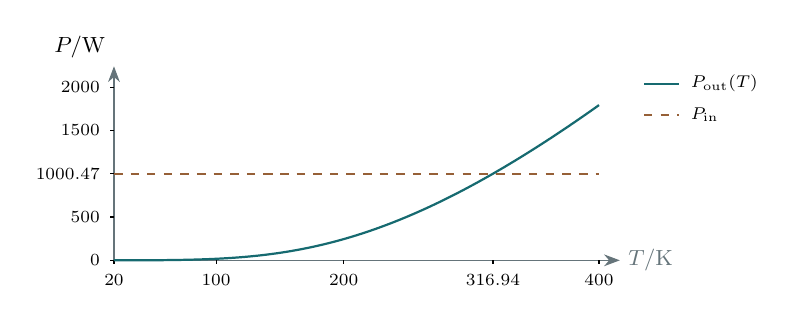
\begin{tikzpicture}[scale=.88,transform shape]
\draw[axis] (0,0.0)--(7.3,0.0) node[right] {$T/\mathrm K$};
\draw[axis] (0,0)--(0,2.8);
\node[above left] at (0,2.8) {$P/\mathrm W$};
\draw[thin] (0.000000,0.0)--(0.000000,-0.06);\node[below,font=\scriptsize] at (0.000000,-0.08) {$ 20 $};
\draw[thin] (1.473684,0.0)--(1.473684,-0.06);\node[below,font=\scriptsize] at (1.473684,-0.08) {$ 100 $};
\draw[thin] (3.315789,0.0)--(3.315789,-0.06);\node[below,font=\scriptsize] at (3.315789,-0.08) {$ 200 $};
\draw[thin] (5.469947,0.0)--(5.469947,-0.06);\node[below,font=\scriptsize] at (5.469947,-0.08) {$ 316.94 $};
\draw[thin] (7.000000,0.0)--(7.000000,-0.06);\node[below,font=\scriptsize] at (7.000000,-0.08) {$ 400 $};
\draw[thin] (0,0.000000)--(-.06,0.000000);\node[left,font=\scriptsize] at (-.08,0.000000) {$ 0 $};
\draw[thin] (0,0.625000)--(-.06,0.625000);\node[left,font=\scriptsize] at (-.08,0.625000) {$ 500 $};
\draw[thin] (0,1.250591)--(-.06,1.250591);\node[left,font=\scriptsize] at (-.08,1.250591) {$ 1000.47 $};
\draw[thin] (0,1.875000)--(-.06,1.875000);\node[left,font=\scriptsize] at (-.08,1.875000) {$ 1500 $};
\draw[thin] (0,2.500000)--(-.06,2.500000);\node[left,font=\scriptsize] at (-.08,2.500000) {$ 2000 $};
\draw[thick,color=accent] plot coordinates {(0.0000000,0.0000356) (0.0291667,0.0000483) (0.0583333,0.0000641) (0.0875000,0.0000835) (0.1166667,0.0001071) (0.1458333,0.0001352) (0.1750000,0.0001686) (0.2041667,0.0002079) (0.2333333,0.0002535) (0.2625000,0.0003064) (0.2916667,0.0003671) (0.3208333,0.0004364) (0.3500000,0.0005151) (0.3791667,0.0006040) (0.4083333,0.0007039) (0.4375000,0.0008157) (0.4666667,0.0009404) (0.4958333,0.0010788) (0.5250000,0.0012320) (0.5541667,0.0014009) (0.5833333,0.0015867) (0.6125000,0.0017903) (0.6416667,0.0020129) (0.6708333,0.0022557) (0.7000000,0.0025197) (0.7291667,0.0028063) (0.7583333,0.0031167) (0.7875000,0.0034522) (0.8166667,0.0038140) (0.8458333,0.0042036) (0.8750000,0.0046222) (0.9041667,0.0050714) (0.9333333,0.0055525) (0.9625000,0.0060670) (0.9916667,0.0066164) (1.0208333,0.0072023) (1.0500000,0.0078262) (1.0791667,0.0084898) (1.1083333,0.0091946) (1.1375000,0.0099422) (1.1666667,0.0107345) (1.1958333,0.0115729) (1.2250000,0.0124594) (1.2541667,0.0133956) (1.2833333,0.0143832) (1.3125000,0.0154241) (1.3416667,0.0165201) (1.3708333,0.0176729) (1.4000000,0.0188844) (1.4291667,0.0201565) (1.4583333,0.0214909) (1.4875000,0.0228895) (1.5166667,0.0243542) (1.5458333,0.0258869) (1.5750000,0.0274894) (1.6041667,0.0291635) (1.6333333,0.0309111) (1.6625000,0.0327341) (1.6916667,0.0346343) (1.7208333,0.0366135) (1.7500000,0.0386735) (1.7791667,0.0408162) (1.8083333,0.0430433) (1.8375000,0.0453567) (1.8666667,0.0477580) (1.8958333,0.0502489) (1.9250000,0.0528313) (1.9541667,0.0555067) (1.9833333,0.0582768) (2.0125000,0.0611433) (2.0416667,0.0641077) (2.0708333,0.0671716) (2.1000000,0.0703365) (2.1291667,0.0736039) (2.1583333,0.0769753) (2.1875000,0.0804521) (2.2166667,0.0840358) (2.2458333,0.0877275) (2.2750000,0.0915287) (2.3041667,0.0954407) (2.3333333,0.0994646) (2.3625000,0.1036018) (2.3916667,0.1078532) (2.4208333,0.1122201) (2.4500000,0.1167035) (2.4791667,0.1213044) (2.5083333,0.1260239) (2.5375000,0.1308629) (2.5666667,0.1358223) (2.5958333,0.1409030) (2.6250000,0.1461058) (2.6541667,0.1514315) (2.6833333,0.1568808) (2.7125000,0.1624544) (2.7416667,0.1681531) (2.7708333,0.1739774) (2.8000000,0.1799279) (2.8291667,0.1860052) (2.8583333,0.1922098) (2.8875000,0.1985421) (2.9166667,0.2050026) (2.9458333,0.2115917) (2.9750000,0.2183098) (3.0041667,0.2251571) (3.0333333,0.2321339) (3.0625000,0.2392406) (3.0916667,0.2464773) (3.1208333,0.2538443) (3.1500000,0.2613416) (3.1791667,0.2689695) (3.2083333,0.2767279) (3.2375000,0.2846170) (3.2666667,0.2926368) (3.2958333,0.3007873) (3.3250000,0.3090685) (3.3541667,0.3174803) (3.3833333,0.3260226) (3.4125000,0.3346954) (3.4416667,0.3434985) (3.4708333,0.3524318) (3.5000000,0.3614951) (3.5291667,0.3706881) (3.5583333,0.3800107) (3.5875000,0.3894626) (3.6166667,0.3990436) (3.6458333,0.4087533) (3.6750000,0.4185915) (3.7041667,0.4285578) (3.7333333,0.4386519) (3.7625000,0.4488734) (3.7916667,0.4592220) (3.8208333,0.4696972) (3.8500000,0.4802987) (3.8791667,0.4910259) (3.9083333,0.5018786) (3.9375000,0.5128561) (3.9666667,0.5239581) (3.9958333,0.5351841) (4.0250000,0.5465335) (4.0541667,0.5580059) (4.0833333,0.5696007) (4.1125000,0.5813175) (4.1416667,0.5931556) (4.1708333,0.6051146) (4.2000000,0.6171938) (4.2291667,0.6293927) (4.2583333,0.6417108) (4.2875000,0.6541474) (4.3166667,0.6667020) (4.3458333,0.6793739) (4.3750000,0.6921625) (4.4041667,0.7050673) (4.4333333,0.7180876) (4.4625000,0.7312229) (4.4916667,0.7444724) (4.5208333,0.7578355) (4.5500000,0.7713116) (4.5791667,0.7849001) (4.6083333,0.7986003) (4.6375000,0.8124115) (4.6666667,0.8263332) (4.6958333,0.8403646) (4.7250000,0.8545051) (4.7541667,0.8687541) (4.7833333,0.8831108) (4.8125000,0.8975746) (4.8416667,0.9121449) (4.8708333,0.9268209) (4.9000000,0.9416021) (4.9291667,0.9564877) (4.9583333,0.9714770) (4.9875000,0.9865695) (5.0166667,1.0017644) (5.0458333,1.0170610) (5.0750000,1.0324587) (5.1041667,1.0479568) (5.1333333,1.0635547) (5.1625000,1.0792517) (5.1916667,1.0950471) (5.2208333,1.1109402) (5.2500000,1.1269303) (5.2791667,1.1430169) (5.3083333,1.1591993) (5.3375000,1.1754767) (5.3666667,1.1918485) (5.3958333,1.2083141) (5.4250000,1.2248728) (5.4541667,1.2415240) (5.4833333,1.2582670) (5.5125000,1.2751011) (5.5416667,1.2920258) (5.5708333,1.3090403) (5.6000000,1.3261440) (5.6291667,1.3433362) (5.6583333,1.3606165) (5.6875000,1.3779840) (5.7166667,1.3954382) (5.7458333,1.4129785) (5.7750000,1.4306041) (5.8041667,1.4483146) (5.8333333,1.4661092) (5.8625000,1.4839874) (5.8916667,1.5019486) (5.9208333,1.5199921) (5.9500000,1.5381173) (5.9791667,1.5563236) (6.0083333,1.5746105) (6.0375000,1.5929772) (6.0666667,1.6114234) (6.0958333,1.6299482) (6.1250000,1.6485513) (6.1541667,1.6672319) (6.1833333,1.6859895) (6.2125000,1.7048235) (6.2416667,1.7237334) (6.2708333,1.7427186) (6.3000000,1.7617785) (6.3291667,1.7809125) (6.3583333,1.8001202) (6.3875000,1.8194009) (6.4166667,1.8387541) (6.4458333,1.8581792) (6.4750000,1.8776758) (6.5041667,1.8972432) (6.5333333,1.9168810) (6.5625000,1.9365885) (6.5916667,1.9563654) (6.6208333,1.9762110) (6.6500000,1.9961249) (6.6791667,2.0161064) (6.7083333,2.0361552) (6.7375000,2.0562707) (6.7666667,2.0764524) (6.7958333,2.0966997) (6.8250000,2.1170123) (6.8541667,2.1373896) (6.8833333,2.1578311) (6.9125000,2.1783363) (6.9416667,2.1989048) (6.9708333,2.2195360) (7.0000000,2.2402296)};
\draw[thick,color=accent] (7.65,2.55)--(8.15,2.55);\node[right,font=\scriptsize] at (8.2,2.55) {$P_{\rm out}(T)$};
\draw[thick,dashed,color=warm] plot coordinates {(0.0000000,1.2505912) (0.0291667,1.2505912) (0.0583333,1.2505912) (0.0875000,1.2505912) (0.1166667,1.2505912) (0.1458333,1.2505912) (0.1750000,1.2505912) (0.2041667,1.2505912) (0.2333333,1.2505912) (0.2625000,1.2505912) (0.2916667,1.2505912) (0.3208333,1.2505912) (0.3500000,1.2505912) (0.3791667,1.2505912) (0.4083333,1.2505912) (0.4375000,1.2505912) (0.4666667,1.2505912) (0.4958333,1.2505912) (0.5250000,1.2505912) (0.5541667,1.2505912) (0.5833333,1.2505912) (0.6125000,1.2505912) (0.6416667,1.2505912) (0.6708333,1.2505912) (0.7000000,1.2505912) (0.7291667,1.2505912) (0.7583333,1.2505912) (0.7875000,1.2505912) (0.8166667,1.2505912) (0.8458333,1.2505912) (0.8750000,1.2505912) (0.9041667,1.2505912) (0.9333333,1.2505912) (0.9625000,1.2505912) (0.9916667,1.2505912) (1.0208333,1.2505912) (1.0500000,1.2505912) (1.0791667,1.2505912) (1.1083333,1.2505912) (1.1375000,1.2505912) (1.1666667,1.2505912) (1.1958333,1.2505912) (1.2250000,1.2505912) (1.2541667,1.2505912) (1.2833333,1.2505912) (1.3125000,1.2505912) (1.3416667,1.2505912) (1.3708333,1.2505912) (1.4000000,1.2505912) (1.4291667,1.2505912) (1.4583333,1.2505912) (1.4875000,1.2505912) (1.5166667,1.2505912) (1.5458333,1.2505912) (1.5750000,1.2505912) (1.6041667,1.2505912) (1.6333333,1.2505912) (1.6625000,1.2505912) (1.6916667,1.2505912) (1.7208333,1.2505912) (1.7500000,1.2505912) (1.7791667,1.2505912) (1.8083333,1.2505912) (1.8375000,1.2505912) (1.8666667,1.2505912) (1.8958333,1.2505912) (1.9250000,1.2505912) (1.9541667,1.2505912) (1.9833333,1.2505912) (2.0125000,1.2505912) (2.0416667,1.2505912) (2.0708333,1.2505912) (2.1000000,1.2505912) (2.1291667,1.2505912) (2.1583333,1.2505912) (2.1875000,1.2505912) (2.2166667,1.2505912) (2.2458333,1.2505912) (2.2750000,1.2505912) (2.3041667,1.2505912) (2.3333333,1.2505912) (2.3625000,1.2505912) (2.3916667,1.2505912) (2.4208333,1.2505912) (2.4500000,1.2505912) (2.4791667,1.2505912) (2.5083333,1.2505912) (2.5375000,1.2505912) (2.5666667,1.2505912) (2.5958333,1.2505912) (2.6250000,1.2505912) (2.6541667,1.2505912) (2.6833333,1.2505912) (2.7125000,1.2505912) (2.7416667,1.2505912) (2.7708333,1.2505912) (2.8000000,1.2505912) (2.8291667,1.2505912) (2.8583333,1.2505912) (2.8875000,1.2505912) (2.9166667,1.2505912) (2.9458333,1.2505912) (2.9750000,1.2505912) (3.0041667,1.2505912) (3.0333333,1.2505912) (3.0625000,1.2505912) (3.0916667,1.2505912) (3.1208333,1.2505912) (3.1500000,1.2505912) (3.1791667,1.2505912) (3.2083333,1.2505912) (3.2375000,1.2505912) (3.2666667,1.2505912) (3.2958333,1.2505912) (3.3250000,1.2505912) (3.3541667,1.2505912) (3.3833333,1.2505912) (3.4125000,1.2505912) (3.4416667,1.2505912) (3.4708333,1.2505912) (3.5000000,1.2505912) (3.5291667,1.2505912) (3.5583333,1.2505912) (3.5875000,1.2505912) (3.6166667,1.2505912) (3.6458333,1.2505912) (3.6750000,1.2505912) (3.7041667,1.2505912) (3.7333333,1.2505912) (3.7625000,1.2505912) (3.7916667,1.2505912) (3.8208333,1.2505912) (3.8500000,1.2505912) (3.8791667,1.2505912) (3.9083333,1.2505912) (3.9375000,1.2505912) (3.9666667,1.2505912) (3.9958333,1.2505912) (4.0250000,1.2505912) (4.0541667,1.2505912) (4.0833333,1.2505912) (4.1125000,1.2505912) (4.1416667,1.2505912) (4.1708333,1.2505912) (4.2000000,1.2505912) (4.2291667,1.2505912) (4.2583333,1.2505912) (4.2875000,1.2505912) (4.3166667,1.2505912) (4.3458333,1.2505912) (4.3750000,1.2505912) (4.4041667,1.2505912) (4.4333333,1.2505912) (4.4625000,1.2505912) (4.4916667,1.2505912) (4.5208333,1.2505912) (4.5500000,1.2505912) (4.5791667,1.2505912) (4.6083333,1.2505912) (4.6375000,1.2505912) (4.6666667,1.2505912) (4.6958333,1.2505912) (4.7250000,1.2505912) (4.7541667,1.2505912) (4.7833333,1.2505912) (4.8125000,1.2505912) (4.8416667,1.2505912) (4.8708333,1.2505912) (4.9000000,1.2505912) (4.9291667,1.2505912) (4.9583333,1.2505912) (4.9875000,1.2505912) (5.0166667,1.2505912) (5.0458333,1.2505912) (5.0750000,1.2505912) (5.1041667,1.2505912) (5.1333333,1.2505912) (5.1625000,1.2505912) (5.1916667,1.2505912) (5.2208333,1.2505912) (5.2500000,1.2505912) (5.2791667,1.2505912) (5.3083333,1.2505912) (5.3375000,1.2505912) (5.3666667,1.2505912) (5.3958333,1.2505912) (5.4250000,1.2505912) (5.4541667,1.2505912) (5.4833333,1.2505912) (5.5125000,1.2505912) (5.5416667,1.2505912) (5.5708333,1.2505912) (5.6000000,1.2505912) (5.6291667,1.2505912) (5.6583333,1.2505912) (5.6875000,1.2505912) (5.7166667,1.2505912) (5.7458333,1.2505912) (5.7750000,1.2505912) (5.8041667,1.2505912) (5.8333333,1.2505912) (5.8625000,1.2505912) (5.8916667,1.2505912) (5.9208333,1.2505912) (5.9500000,1.2505912) (5.9791667,1.2505912) (6.0083333,1.2505912) (6.0375000,1.2505912) (6.0666667,1.2505912) (6.0958333,1.2505912) (6.1250000,1.2505912) (6.1541667,1.2505912) (6.1833333,1.2505912) (6.2125000,1.2505912) (6.2416667,1.2505912) (6.2708333,1.2505912) (6.3000000,1.2505912) (6.3291667,1.2505912) (6.3583333,1.2505912) (6.3875000,1.2505912) (6.4166667,1.2505912) (6.4458333,1.2505912) (6.4750000,1.2505912) (6.5041667,1.2505912) (6.5333333,1.2505912) (6.5625000,1.2505912) (6.5916667,1.2505912) (6.6208333,1.2505912) (6.6500000,1.2505912) (6.6791667,1.2505912) (6.7083333,1.2505912) (6.7375000,1.2505912) (6.7666667,1.2505912) (6.7958333,1.2505912) (6.8250000,1.2505912) (6.8541667,1.2505912) (6.8833333,1.2505912) (6.9125000,1.2505912) (6.9416667,1.2505912) (6.9708333,1.2505912) (7.0000000,1.2505912)};
\draw[thick,dashed,color=warm] (7.65,2.0999999999999996)--(8.15,2.0999999999999996);\node[right,font=\scriptsize] at (8.2,2.0999999999999996) {$P_{\rm in}$};
\end{tikzpicture}
\figcaption{解图近1.7C\quad 允许发射功率与1000瓦内部热源加太阳吸收的平衡交点}
\end{minipage}\end{center}
\begin{center}\begin{minipage}{.98\linewidth}\centering
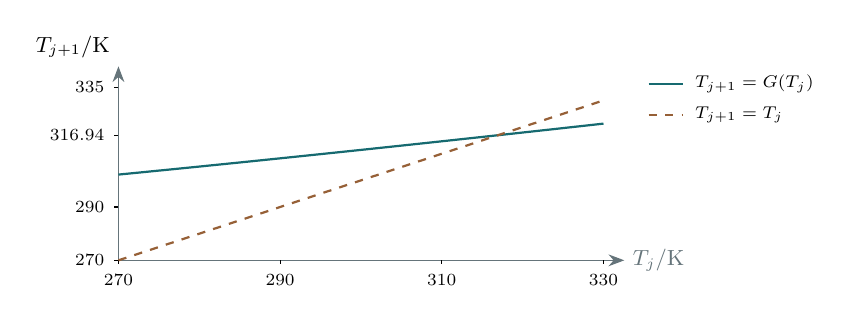
\begin{tikzpicture}[scale=.88,transform shape]
\draw[axis] (0,0)--(7.3,0) node[right] {$T_j/\mathrm K$};
\draw[axis] (0,0)--(0,2.8);
\node[above left] at (0,2.8) {$T_{j+1}/\mathrm K$};
\draw[thin] (0.000000,0)--(0.000000,-0.06);\node[below,font=\scriptsize] at (0.000000,-0.08) {$ 270 $};
\draw[thin] (2.333333,0)--(2.333333,-0.06);\node[below,font=\scriptsize] at (2.333333,-0.08) {$ 290 $};
\draw[thin] (4.666667,0)--(4.666667,-0.06);\node[below,font=\scriptsize] at (4.666667,-0.08) {$ 310 $};
\draw[thin] (7.000000,0)--(7.000000,-0.06);\node[below,font=\scriptsize] at (7.000000,-0.08) {$ 330 $};
\draw[thin] (0,0.000000)--(-.06,0.000000);\node[left,font=\scriptsize] at (-.08,0.000000) {$ 270 $};
\draw[thin] (0,0.769231)--(-.06,0.769231);\node[left,font=\scriptsize] at (-.08,0.769231) {$ 290 $};
\draw[thin] (0,1.805385)--(-.06,1.805385);\node[left,font=\scriptsize] at (-.08,1.805385) {$ 316.94 $};
\draw[thin] (0,2.500000)--(-.06,2.500000);\node[left,font=\scriptsize] at (-.08,2.500000) {$ 335 $};
\draw[thick,color=accent] plot coordinates {(0.0000000,1.2374644) (0.0291667,1.2403169) (0.0583333,1.2431715) (0.0875000,1.2460282) (0.1166667,1.2488871) (0.1458333,1.2517482) (0.1750000,1.2546114) (0.2041667,1.2574767) (0.2333333,1.2603442) (0.2625000,1.2632138) (0.2916667,1.2660855) (0.3208333,1.2689593) (0.3500000,1.2718353) (0.3791667,1.2747133) (0.4083333,1.2775935) (0.4375000,1.2804757) (0.4666667,1.2833600) (0.4958333,1.2862464) (0.5250000,1.2891349) (0.5541667,1.2920254) (0.5833333,1.2949180) (0.6125000,1.2978127) (0.6416667,1.3007094) (0.6708333,1.3036081) (0.7000000,1.3065090) (0.7291667,1.3094118) (0.7583333,1.3123167) (0.7875000,1.3152236) (0.8166667,1.3181325) (0.8458333,1.3210434) (0.8750000,1.3239564) (0.9041667,1.3268713) (0.9333333,1.3297883) (0.9625000,1.3327072) (0.9916667,1.3356281) (1.0208333,1.3385510) (1.0500000,1.3414759) (1.0791667,1.3444028) (1.1083333,1.3473316) (1.1375000,1.3502624) (1.1666667,1.3531952) (1.1958333,1.3561299) (1.2250000,1.3590665) (1.2541667,1.3620051) (1.2833333,1.3649457) (1.3125000,1.3678881) (1.3416667,1.3708325) (1.3708333,1.3737788) (1.4000000,1.3767270) (1.4291667,1.3796772) (1.4583333,1.3826292) (1.4875000,1.3855832) (1.5166667,1.3885390) (1.5458333,1.3914967) (1.5750000,1.3944563) (1.6041667,1.3974178) (1.6333333,1.4003812) (1.6625000,1.4033464) (1.6916667,1.4063135) (1.7208333,1.4092825) (1.7500000,1.4122533) (1.7791667,1.4152260) (1.8083333,1.4182005) (1.8375000,1.4211768) (1.8666667,1.4241550) (1.8958333,1.4271351) (1.9250000,1.4301169) (1.9541667,1.4331006) (1.9833333,1.4360860) (2.0125000,1.4390733) (2.0416667,1.4420624) (2.0708333,1.4450533) (2.1000000,1.4480460) (2.1291667,1.4510405) (2.1583333,1.4540368) (2.1875000,1.4570349) (2.2166667,1.4600347) (2.2458333,1.4630363) (2.2750000,1.4660397) (2.3041667,1.4690448) (2.3333333,1.4720517) (2.3625000,1.4750604) (2.3916667,1.4780708) (2.4208333,1.4810829) (2.4500000,1.4840968) (2.4791667,1.4871124) (2.5083333,1.4901298) (2.5375000,1.4931489) (2.5666667,1.4961697) (2.5958333,1.4991922) (2.6250000,1.5022164) (2.6541667,1.5052423) (2.6833333,1.5082700) (2.7125000,1.5112993) (2.7416667,1.5143303) (2.7708333,1.5173631) (2.8000000,1.5203975) (2.8291667,1.5234335) (2.8583333,1.5264713) (2.8875000,1.5295107) (2.9166667,1.5325518) (2.9458333,1.5355946) (2.9750000,1.5386390) (3.0041667,1.5416851) (3.0333333,1.5447328) (3.0625000,1.5477821) (3.0916667,1.5508331) (3.1208333,1.5538858) (3.1500000,1.5569400) (3.1791667,1.5599959) (3.2083333,1.5630534) (3.2375000,1.5661126) (3.2666667,1.5691733) (3.2958333,1.5722356) (3.3250000,1.5752996) (3.3541667,1.5783652) (3.3833333,1.5814323) (3.4125000,1.5845011) (3.4416667,1.5875714) (3.4708333,1.5906433) (3.5000000,1.5937168) (3.5291667,1.5967919) (3.5583333,1.5998685) (3.5875000,1.6029467) (3.6166667,1.6060265) (3.6458333,1.6091078) (3.6750000,1.6121907) (3.7041667,1.6152751) (3.7333333,1.6183610) (3.7625000,1.6214486) (3.7916667,1.6245376) (3.8208333,1.6276282) (3.8500000,1.6307203) (3.8791667,1.6338139) (3.9083333,1.6369091) (3.9375000,1.6400057) (3.9666667,1.6431039) (3.9958333,1.6462036) (4.0250000,1.6493048) (4.0541667,1.6524075) (4.0833333,1.6555117) (4.1125000,1.6586173) (4.1416667,1.6617245) (4.1708333,1.6648331) (4.2000000,1.6679433) (4.2291667,1.6710549) (4.2583333,1.6741679) (4.2875000,1.6772825) (4.3166667,1.6803985) (4.3458333,1.6835159) (4.3750000,1.6866349) (4.4041667,1.6897552) (4.4333333,1.6928770) (4.4625000,1.6960003) (4.4916667,1.6991250) (4.5208333,1.7022511) (4.5500000,1.7053787) (4.5791667,1.7085077) (4.6083333,1.7116381) (4.6375000,1.7147700) (4.6666667,1.7179032) (4.6958333,1.7210379) (4.7250000,1.7241740) (4.7541667,1.7273114) (4.7833333,1.7304503) (4.8125000,1.7335906) (4.8416667,1.7367323) (4.8708333,1.7398753) (4.9000000,1.7430198) (4.9291667,1.7461656) (4.9583333,1.7493128) (4.9875000,1.7524614) (5.0166667,1.7556113) (5.0458333,1.7587627) (5.0750000,1.7619153) (5.1041667,1.7650694) (5.1333333,1.7682248) (5.1625000,1.7713815) (5.1916667,1.7745396) (5.2208333,1.7776991) (5.2500000,1.7808599) (5.2791667,1.7840220) (5.3083333,1.7871854) (5.3375000,1.7903502) (5.3666667,1.7935163) (5.3958333,1.7966838) (5.4250000,1.7998525) (5.4541667,1.8030226) (5.4833333,1.8061940) (5.5125000,1.8093667) (5.5416667,1.8125407) (5.5708333,1.8157160) (5.6000000,1.8188926) (5.6291667,1.8220704) (5.6583333,1.8252496) (5.6875000,1.8284301) (5.7166667,1.8316118) (5.7458333,1.8347949) (5.7750000,1.8379792) (5.8041667,1.8411648) (5.8333333,1.8443516) (5.8625000,1.8475397) (5.8916667,1.8507291) (5.9208333,1.8539197) (5.9500000,1.8571116) (5.9791667,1.8603048) (6.0083333,1.8634992) (6.0375000,1.8666948) (6.0666667,1.8698917) (6.0958333,1.8730898) (6.1250000,1.8762892) (6.1541667,1.8794898) (6.1833333,1.8826916) (6.2125000,1.8858946) (6.2416667,1.8890989) (6.2708333,1.8923044) (6.3000000,1.8955111) (6.3291667,1.8987190) (6.3583333,1.9019281) (6.3875000,1.9051384) (6.4166667,1.9083500) (6.4458333,1.9115627) (6.4750000,1.9147766) (6.5041667,1.9179917) (6.5333333,1.9212080) (6.5625000,1.9244255) (6.5916667,1.9276442) (6.6208333,1.9308640) (6.6500000,1.9340851) (6.6791667,1.9373073) (6.7083333,1.9405306) (6.7375000,1.9437552) (6.7666667,1.9469808) (6.7958333,1.9502077) (6.8250000,1.9534357) (6.8541667,1.9566649) (6.8833333,1.9598952) (6.9125000,1.9631266) (6.9416667,1.9663593) (6.9708333,1.9695930) (7.0000000,1.9728279)};
\draw[thick,color=accent] (7.65,2.55)--(8.15,2.55);\node[right,font=\scriptsize] at (8.2,2.55) {$T_{j+1}=G(T_j)$};
\draw[thick,dashed,color=warm] plot coordinates {(0.0000000,0.0000000) (0.0291667,0.0096154) (0.0583333,0.0192308) (0.0875000,0.0288462) (0.1166667,0.0384615) (0.1458333,0.0480769) (0.1750000,0.0576923) (0.2041667,0.0673077) (0.2333333,0.0769231) (0.2625000,0.0865385) (0.2916667,0.0961538) (0.3208333,0.1057692) (0.3500000,0.1153846) (0.3791667,0.1250000) (0.4083333,0.1346154) (0.4375000,0.1442308) (0.4666667,0.1538462) (0.4958333,0.1634615) (0.5250000,0.1730769) (0.5541667,0.1826923) (0.5833333,0.1923077) (0.6125000,0.2019231) (0.6416667,0.2115385) (0.6708333,0.2211538) (0.7000000,0.2307692) (0.7291667,0.2403846) (0.7583333,0.2500000) (0.7875000,0.2596154) (0.8166667,0.2692308) (0.8458333,0.2788462) (0.8750000,0.2884615) (0.9041667,0.2980769) (0.9333333,0.3076923) (0.9625000,0.3173077) (0.9916667,0.3269231) (1.0208333,0.3365385) (1.0500000,0.3461538) (1.0791667,0.3557692) (1.1083333,0.3653846) (1.1375000,0.3750000) (1.1666667,0.3846154) (1.1958333,0.3942308) (1.2250000,0.4038462) (1.2541667,0.4134615) (1.2833333,0.4230769) (1.3125000,0.4326923) (1.3416667,0.4423077) (1.3708333,0.4519231) (1.4000000,0.4615385) (1.4291667,0.4711538) (1.4583333,0.4807692) (1.4875000,0.4903846) (1.5166667,0.5000000) (1.5458333,0.5096154) (1.5750000,0.5192308) (1.6041667,0.5288462) (1.6333333,0.5384615) (1.6625000,0.5480769) (1.6916667,0.5576923) (1.7208333,0.5673077) (1.7500000,0.5769231) (1.7791667,0.5865385) (1.8083333,0.5961538) (1.8375000,0.6057692) (1.8666667,0.6153846) (1.8958333,0.6250000) (1.9250000,0.6346154) (1.9541667,0.6442308) (1.9833333,0.6538462) (2.0125000,0.6634615) (2.0416667,0.6730769) (2.0708333,0.6826923) (2.1000000,0.6923077) (2.1291667,0.7019231) (2.1583333,0.7115385) (2.1875000,0.7211538) (2.2166667,0.7307692) (2.2458333,0.7403846) (2.2750000,0.7500000) (2.3041667,0.7596154) (2.3333333,0.7692308) (2.3625000,0.7788462) (2.3916667,0.7884615) (2.4208333,0.7980769) (2.4500000,0.8076923) (2.4791667,0.8173077) (2.5083333,0.8269231) (2.5375000,0.8365385) (2.5666667,0.8461538) (2.5958333,0.8557692) (2.6250000,0.8653846) (2.6541667,0.8750000) (2.6833333,0.8846154) (2.7125000,0.8942308) (2.7416667,0.9038462) (2.7708333,0.9134615) (2.8000000,0.9230769) (2.8291667,0.9326923) (2.8583333,0.9423077) (2.8875000,0.9519231) (2.9166667,0.9615385) (2.9458333,0.9711538) (2.9750000,0.9807692) (3.0041667,0.9903846) (3.0333333,1.0000000) (3.0625000,1.0096154) (3.0916667,1.0192308) (3.1208333,1.0288462) (3.1500000,1.0384615) (3.1791667,1.0480769) (3.2083333,1.0576923) (3.2375000,1.0673077) (3.2666667,1.0769231) (3.2958333,1.0865385) (3.3250000,1.0961538) (3.3541667,1.1057692) (3.3833333,1.1153846) (3.4125000,1.1250000) (3.4416667,1.1346154) (3.4708333,1.1442308) (3.5000000,1.1538462) (3.5291667,1.1634615) (3.5583333,1.1730769) (3.5875000,1.1826923) (3.6166667,1.1923077) (3.6458333,1.2019231) (3.6750000,1.2115385) (3.7041667,1.2211538) (3.7333333,1.2307692) (3.7625000,1.2403846) (3.7916667,1.2500000) (3.8208333,1.2596154) (3.8500000,1.2692308) (3.8791667,1.2788462) (3.9083333,1.2884615) (3.9375000,1.2980769) (3.9666667,1.3076923) (3.9958333,1.3173077) (4.0250000,1.3269231) (4.0541667,1.3365385) (4.0833333,1.3461538) (4.1125000,1.3557692) (4.1416667,1.3653846) (4.1708333,1.3750000) (4.2000000,1.3846154) (4.2291667,1.3942308) (4.2583333,1.4038462) (4.2875000,1.4134615) (4.3166667,1.4230769) (4.3458333,1.4326923) (4.3750000,1.4423077) (4.4041667,1.4519231) (4.4333333,1.4615385) (4.4625000,1.4711538) (4.4916667,1.4807692) (4.5208333,1.4903846) (4.5500000,1.5000000) (4.5791667,1.5096154) (4.6083333,1.5192308) (4.6375000,1.5288462) (4.6666667,1.5384615) (4.6958333,1.5480769) (4.7250000,1.5576923) (4.7541667,1.5673077) (4.7833333,1.5769231) (4.8125000,1.5865385) (4.8416667,1.5961538) (4.8708333,1.6057692) (4.9000000,1.6153846) (4.9291667,1.6250000) (4.9583333,1.6346154) (4.9875000,1.6442308) (5.0166667,1.6538462) (5.0458333,1.6634615) (5.0750000,1.6730769) (5.1041667,1.6826923) (5.1333333,1.6923077) (5.1625000,1.7019231) (5.1916667,1.7115385) (5.2208333,1.7211538) (5.2500000,1.7307692) (5.2791667,1.7403846) (5.3083333,1.7500000) (5.3375000,1.7596154) (5.3666667,1.7692308) (5.3958333,1.7788462) (5.4250000,1.7884615) (5.4541667,1.7980769) (5.4833333,1.8076923) (5.5125000,1.8173077) (5.5416667,1.8269231) (5.5708333,1.8365385) (5.6000000,1.8461538) (5.6291667,1.8557692) (5.6583333,1.8653846) (5.6875000,1.8750000) (5.7166667,1.8846154) (5.7458333,1.8942308) (5.7750000,1.9038462) (5.8041667,1.9134615) (5.8333333,1.9230769) (5.8625000,1.9326923) (5.8916667,1.9423077) (5.9208333,1.9519231) (5.9500000,1.9615385) (5.9791667,1.9711538) (6.0083333,1.9807692) (6.0375000,1.9903846) (6.0666667,2.0000000) (6.0958333,2.0096154) (6.1250000,2.0192308) (6.1541667,2.0288462) (6.1833333,2.0384615) (6.2125000,2.0480769) (6.2416667,2.0576923) (6.2708333,2.0673077) (6.3000000,2.0769231) (6.3291667,2.0865385) (6.3583333,2.0961538) (6.3875000,2.1057692) (6.4166667,2.1153846) (6.4458333,2.1250000) (6.4750000,2.1346154) (6.5041667,2.1442308) (6.5333333,2.1538462) (6.5625000,2.1634615) (6.5916667,2.1730769) (6.6208333,2.1826923) (6.6500000,2.1923077) (6.6791667,2.2019231) (6.7083333,2.2115385) (6.7375000,2.2211538) (6.7666667,2.2307692) (6.7958333,2.2403846) (6.8250000,2.2500000) (6.8541667,2.2596154) (6.8833333,2.2692308) (6.9125000,2.2788462) (6.9416667,2.2884615) (6.9708333,2.2980769) (7.0000000,2.3076923)};
\draw[thick,dashed,color=warm] (7.65,2.0999999999999996)--(8.15,2.0999999999999996);\node[right,font=\scriptsize] at (8.2,2.0999999999999996) {$T_{j+1}=T_j$};
\end{tikzpicture}
\figcaption{解图近1.7D\quad 温度相关截止份额在迭代中更新至自洽交点}
\end{minipage}\end{center}
还可从谱直接说明平衡的唯一性。对每个固定允许频率，$M_f(T)$中的$e^{hf/(k_BT)}-1$随温度升高而减小，所以$M_f(T)$严格增加。积分上限$f_c$固定，允许发射总功率也严格增加；在同一输入功率下仅有一个平衡交点。温度稍高时，净散热大于输入；稍低时，输入大于散热，因此这一热平衡稳定。
在上述交点附近，还可直接读出温度迭代的收敛速度。记$x=1200/T$，由$F'(x)=p(x)$得
\[
 \frac{\dd P_{\rm out}}{\dd T}
 =4\pi a^2\sigma T^3[4F(x)-xp(x)].
\]
对$t^4/(e^t-1)$求导后从0积分到$x$，可将方括号写成正积分：
\[
 4F(x)-xp(x)=\frac{15}{\pi^4}
 \int_0^x\frac{t^4e^t}{(e^t-1)^2}\dd t>0.
\]
因此在固定点$T_*=G(T_*)$处，更新函数的斜率满足
\[
 G'(T_*)=\frac{x_*p(x_*)}{4F(x_*)}\simeq0.330,
 \qquad 0<G'(T_*)<1.
\]
若$T_j=T_*+\delta T_j$，一阶展开给$\delta T_{j+1}\simeq0.330\,\delta T_j$。解图近1.7D的更新曲线在交点处比自洽直线平缓，表中后几步的温差也按这一比例缩小。

（4）广告把所有频率的高反射和黑体发射同时赋给同一被动涂层。对不透光表面，$\alpha_f=1-R_f$；$R_f>0.9$给$\alpha_f<0.1$，Kirchhoff关系则给对应$\varepsilon_f<0.1$，与全频$\varepsilon_f=1$的黑体发射互不相容。这一矛盾在同温辐射腔中最直接：表面吸收和发射的每个频段在平衡时逐频相等，广告系数却给净能量持续离开同温物体。

也可按第二定律看热流方向。设物体周围是温度$T_0$的大黑体腔，若仍按广告令它以黑体强度发射而最多吸收十分之一腔辐射，在物体温度为$0.9T_0$时会有$q_{\rm out}\ge\sigma T_0^4(0.9^4-0.1)>0$。这意味着物体低于环境温度时仍把净热量送给较热环境，构成自发的低温向高温输热。所宣称的系数组合同时违反同频热平衡关系和第二定律。

（5）要使相同球体的太阳平衡温度高于黑体结果，让涂层在太阳主要波段吸收较强、在自身热红外波段发射较弱。太阳谱温度6000K、卫星热谱约数百K，两种频段权重不同。定义太阳谱平均吸收率$\alpha_s=\int\alpha_fM_f(T_s)\dd f/(\sigma T_s^4)$，自身热谱平均发射率$\varepsilon_T=\int\varepsilon_fM_f(T)\dd f/(\sigma T^4)$，无内部热源的平衡为
\[
\alpha_s\pi a^2S=4\pi a^2\varepsilon_T\sigma T^4,\qquad
T=T_b(\alpha_s/\varepsilon_T)^{1/4}.
\]
所以所求条件是在实际平衡温度处$\alpha_s/\varepsilon_T>1$。各频率仍满足$\alpha_f=\varepsilon_f$，两个平均值的差由不同辐射谱的权重形成。内部多次吸收和再发射重新分配能量，整体平衡中的外部输入仍为吸收的太阳功率；较弱的热红外发射使物体升温，直到总出射功率与该输入相等。


\Needspace{13\baselineskip}

\pdfbookmark[2]{第 8 题 由光电子磁轨道求逸出功}{q8}

\section*{第 8 题\quad 由光电子磁轨道求逸出功}\label{q:8}

波长350nm的光照射光电材料，逸出电子中动量最大的电子垂直进入$B=1.50\times10^{-5}\,\mathrm T$的匀强磁场，沿半径$r=18.0\,\mathrm{cm}$的圆轨道运动。磁场前无额外电势加速，求材料逸出功，检查所用电子动能近似。

\begin{center}\begin{minipage}{.98\linewidth}\centering
\begin{tikzpicture}[scale=.9,transform shape]
\draw[object] (0.00000,-1.80000)--(0.00000,1.10000);\node[above] at (0.00000,1.20000) {材料};\draw[traj] plot coordinates {(-2.00000,1.00000) (-1.98150,1.00939) (-1.96342,1.01737) (-1.94616,1.02263) (-1.93000,1.02421) (-1.91514,1.02147) (-1.90162,1.01426) (-1.88935,1.00288) (-1.87812,0.98806) (-1.86758,0.97089) (-1.85735,0.95271) (-1.84699,0.93496) (-1.83609,0.91903) (-1.82427,0.90614) (-1.81128,0.89716) (-1.79697,0.89259) (-1.78133,0.89246) (-1.76449,0.89632) (-1.74670,0.90333) (-1.72832,0.91231) (-1.70977,0.92188) (-1.69147,0.93060) (-1.67383,0.93711) (-1.65720,0.94028) (-1.64179,0.93935) (-1.62773,0.93396) (-1.61497,0.92421) (-1.60334,0.91068) (-1.59257,0.89432) (-1.58226,0.87638) (-1.57201,0.85828) (-1.56138,0.84145) (-1.54997,0.82719) (-1.53749,0.81653) (-1.52372,0.81014) (-1.50861,0.80822) (-1.49224,0.81053) (-1.47480,0.81638) (-1.45661,0.82472) (-1.43808,0.83422) (-1.41962,0.84346) (-1.40167,0.85102) (-1.38459,0.85567) (-1.36867,0.85649) (-1.35405,0.85293) (-1.34077,0.84491) (-1.32871,0.83283) (-1.31763,0.81749) (-1.30719,0.80003) (-1.29696,0.78182) (-1.28654,0.76430) (-1.27549,0.74885) (-1.26347,0.73662) (-1.25025,0.72843) (-1.23569,0.72469) (-1.21981,0.72534) (-1.20277,0.72985) (-1.18485,0.73732) (-1.16641,0.74651) (-1.14787,0.75604) (-1.12966,0.76444) (-1.11218,0.77042) (-1.09576,0.77289) (-1.08060,0.77115) (-1.06678,0.76493) (-1.05425,0.75443) (-1.04280,0.74030) (-1.03214,0.72355) (-1.02188,0.70547) (-1.01159,0.68750) (-1.00084,0.67105) (-0.98926,0.65739) (-0.97655,0.64747) (-0.96254,0.64190) (-0.94719,0.64079) (-0.93060,0.64382) (-0.91299,0.65021) (-0.89471,0.65887) (-0.87616,0.66843) (-0.85777,0.67746) (-0.83995,0.68457) (-0.82307,0.68858) (-0.80737,0.68862) (-0.79300,0.68423) (-0.77996,0.67543) (-0.76810,0.66267) (-0.75717,0.64685) (-0.74680,0.62914) (-0.73657,0.61095) (-0.72606,0.59372) (-0.71486,0.57878) (-0.70263,0.56724) (-0.68917,0.55986) (-0.67436,0.55694) (-0.65825,0.55835) (-0.64103,0.56348) (-0.62298,0.57137) (-0.60449,0.58073) (-0.58597,0.59016) (-0.56788,0.59821) (-0.55057,0.60361) (-0.53437,0.60534) (-0.51945,0.60279) (-0.50588,0.59576) (-0.49356,0.58453) (-0.48229,0.56983) (-0.47173,0.55273) (-0.46150,0.53457) (-0.45116,0.51677) (-0.44028,0.50074) (-0.42851,0.48771) (-0.41557,0.47856) (-0.40131,0.47381) (-0.38572,0.47350) (-0.36892,0.47722) (-0.35117,0.48412) (-0.33281,0.49305) (-0.31425,0.50262) (-0.29593,0.51140) (-0.27826,0.51802) (-0.26158,0.52135) (-0.24612,0.52060) (-0.23200,0.51538) (-0.21919,0.50581) (-0.20753,0.49241) (-0.19673,0.47614) (-0.18641,0.45824) (-0.17617,0.44012) (-0.16555,0.42321) (-0.15419,0.40882) (-0.14175,0.39801) (-0.12804,0.39143) (-0.11298,0.38933) (-0.09666,0.39148) (-0.07925,0.39721) (-0.06109,0.40547) (-0.04256,0.41495) (-0.02410,0.42423) (-0.00612,0.43188) (0.01100,0.43668)};\draw[motion] (-0.17241,0.45172)--(0.00000,0.40000);\node[above] at (-1.00000,0.70000) {350nm};\draw[motion] (0.00000,0.00000)--(2.50000,0.00000);\draw[traj] plot coordinates {(2.50000,0.00000) (2.54751,-0.00094) (2.59494,-0.00376) (2.64222,-0.00846) (2.68929,-0.01502) (2.73605,-0.02345) (2.78244,-0.03371) (2.82840,-0.04581) (2.87383,-0.05972) (2.91868,-0.07541) (2.96288,-0.09287) (3.00634,-0.11206) (3.04902,-0.13296) (3.09083,-0.15553) (3.13172,-0.17974) (3.17162,-0.20555) (3.21046,-0.23292) (3.24819,-0.26180) (3.28474,-0.29216) (3.32007,-0.32394) (3.35411,-0.35709) (3.38681,-0.39157) (3.41812,-0.42731) (3.44799,-0.46426) (3.47638,-0.50237) (3.50323,-0.54157) (3.52851,-0.58180) (3.55218,-0.62301) (3.57420,-0.66511) (3.59453,-0.70806) (3.61315,-0.75178) (3.63002,-0.79620) (3.64512,-0.84125) (3.65842,-0.88687) (3.66991,-0.93297) (3.67957,-0.97950) (3.68737,-1.02637) (3.69332,-1.07352) (3.69739,-1.12086) (3.69958,-1.16832) (3.69990,-1.21584) (3.69833,-1.26333) (3.69488,-1.31072) (3.68956,-1.35794) (3.68238,-1.40491) (3.67334,-1.45156) (3.66246,-1.49781) (3.64976,-1.54360) (3.63525,-1.58885) (3.61897,-1.63349) (3.60093,-1.67745) (3.58116,-1.72066) (3.55970,-1.76306) (3.53658,-1.80457) (3.51183,-1.84513) (3.48550,-1.88468) (3.45762,-1.92316) (3.42824,-1.96051) (3.39740,-1.99666) (3.36516,-2.03156) (3.33156,-2.06516) (3.29666,-2.09740) (3.26051,-2.12824) (3.22316,-2.15762) (3.18468,-2.18550) (3.14513,-2.21183) (3.10457,-2.23658) (3.06306,-2.25970) (3.02066,-2.28116) (2.97745,-2.30093) (2.93349,-2.31897) (2.88885,-2.33525) (2.84360,-2.34976) (2.79781,-2.36246) (2.75156,-2.37334) (2.70491,-2.38238) (2.65794,-2.38956) (2.61072,-2.39488) (2.56333,-2.39833) (2.51584,-2.39990) (2.46832,-2.39958) (2.42086,-2.39739) (2.37352,-2.39332) (2.32637,-2.38737) (2.27950,-2.37957) (2.23297,-2.36991) (2.18687,-2.35842) (2.14125,-2.34512) (2.09620,-2.33002) (2.05178,-2.31315) (2.00806,-2.29453) (1.96511,-2.27420) (1.92301,-2.25218) (1.88180,-2.22851) (1.84157,-2.20323) (1.80237,-2.17638) (1.76426,-2.14799) (1.72731,-2.11812) (1.69157,-2.08681) (1.65709,-2.05411) (1.62394,-2.02007) (1.59216,-1.98474) (1.56180,-1.94819) (1.53292,-1.91046) (1.50555,-1.87162) (1.47974,-1.83172) (1.45553,-1.79083) (1.43296,-1.74902) (1.41206,-1.70634) (1.39287,-1.66288) (1.37541,-1.61868) (1.35972,-1.57383) (1.34581,-1.52840) (1.33371,-1.48244) (1.32345,-1.43605) (1.31502,-1.38929) (1.30846,-1.34222) (1.30376,-1.29494) (1.30094,-1.24751) (1.30000,-1.20000)};\draw[motion] (3.68000,-1.00000)--(3.68000,-1.35000);\draw[<->,thin,color=muted] (2.50000,-1.20000)--(1.30000,-1.20000);\node[below] at (1.90000,-1.20000) {$r$};\draw[force] (2.50000,0.00000)--(2.50000,-0.65000);\node[right] at (2.70000,-0.50000) {$\boldsymbol F_B$};\node[above] at (1.20000,-1.80000) {$\otimes$};\node[above] at (1.20000,-0.30000) {$\otimes$};\node[above] at (4.30000,-1.80000) {$\otimes$};\node[above] at (4.30000,-0.30000) {$\otimes$};\node[above] at (4.50000,1.00000) {$B$入纸面};\node[above] at (0.80000,0.25000) {$\boldsymbol p$};
\end{tikzpicture}
\figcaption{图近1.8\quad 光电子逸出后进入匀强磁场，磁力不做功。}
\end{minipage}\end{center}

\Needspace{6\baselineskip}\subsection*{解答}


图近1.8中，最高能量光电子离开材料后垂直进入匀强磁场，中途无电势加速。洛伦兹力为$-e\boldsymbol v\times\boldsymbol B$，它与速度垂直，故磁场改变运动方向而保持动能。解图近1.8A取磁场入纸面，电子在圆顶端向右运动，负电荷所受磁力向下指向圆心，轨道沿顺时针弯曲。

匀速圆周运动中，动量矢量大小不变，方向每秒转过$v/r$，所以其变化率大小为$pv/r$。与磁力大小$evB$相等，
\[
\frac{pv}{r}=evB,\qquad \boxed{p=eBr}.
\]
该式测得的是垂直磁场的动量。本题电子垂直入射，使$p_\perp=p$；若另给斜入射方向，则$p_\perp=eBr$与平行动量共同决定总动能。先由题设轨道求完整动量，再选择对应能量表达式。
\begin{center}\begin{minipage}{.98\linewidth}\centering
\begin{tikzpicture}[scale=.95,transform shape]
\draw[thick,color=accent] plot coordinates {(0.0000000,1.5000000) (0.0785039,1.4979443) (0.1567927,1.4917828) (0.2346517,1.4815325) (0.3118675,1.4672214) (0.3882286,1.4488887) (0.4635255,1.4265848) (0.5375519,1.4003706) (0.6101050,1.3703182) (0.6809857,1.3365098) (0.7500000,1.2990381) (0.8169586,1.2580059) (0.8816779,1.2135255) (0.9439806,1.1657189) (1.0036959,1.1147172) (1.0606602,1.0606602) (1.1147172,1.0036959) (1.1657189,0.9439806) (1.2135255,0.8816779) (1.2580059,0.8169586) (1.2990381,0.7500000) (1.3365098,0.6809857) (1.3703182,0.6101050) (1.4003706,0.5375519) (1.4265848,0.4635255) (1.4488887,0.3882286) (1.4672214,0.3118675) (1.4815325,0.2346517) (1.4917828,0.1567927) (1.4979443,0.0785039) (1.5000000,0.0000000) (1.4979443,-0.0785039) (1.4917828,-0.1567927) (1.4815325,-0.2346517) (1.4672214,-0.3118675) (1.4488887,-0.3882286) (1.4265848,-0.4635255) (1.4003706,-0.5375519) (1.3703182,-0.6101050) (1.3365098,-0.6809857) (1.2990381,-0.7500000) (1.2580059,-0.8169586) (1.2135255,-0.8816779) (1.1657189,-0.9439806) (1.1147172,-1.0036959) (1.0606602,-1.0606602) (1.0036959,-1.1147172) (0.9439806,-1.1657189) (0.8816779,-1.2135255) (0.8169586,-1.2580059) (0.7500000,-1.2990381) (0.6809857,-1.3365098) (0.6101050,-1.3703182) (0.5375519,-1.4003706) (0.4635255,-1.4265848) (0.3882286,-1.4488887) (0.3118675,-1.4672214) (0.2346517,-1.4815325) (0.1567927,-1.4917828) (0.0785039,-1.4979443) (0.0000000,-1.5000000) (-0.0785039,-1.4979443) (-0.1567927,-1.4917828) (-0.2346517,-1.4815325) (-0.3118675,-1.4672214) (-0.3882286,-1.4488887) (-0.4635255,-1.4265848) (-0.5375519,-1.4003706) (-0.6101050,-1.3703182) (-0.6809857,-1.3365098) (-0.7500000,-1.2990381) (-0.8169586,-1.2580059) (-0.8816779,-1.2135255) (-0.9439806,-1.1657189) (-1.0036959,-1.1147172) (-1.0606602,-1.0606602) (-1.1147172,-1.0036959) (-1.1657189,-0.9439806) (-1.2135255,-0.8816779) (-1.2580059,-0.8169586) (-1.2990381,-0.7500000) (-1.3365098,-0.6809857) (-1.3703182,-0.6101050) (-1.4003706,-0.5375519) (-1.4265848,-0.4635255) (-1.4488887,-0.3882286) (-1.4672214,-0.3118675) (-1.4815325,-0.2346517) (-1.4917828,-0.1567927) (-1.4979443,-0.0785039) (-1.5000000,-0.0000000) (-1.4979443,0.0785039) (-1.4917828,0.1567927) (-1.4815325,0.2346517) (-1.4672214,0.3118675) (-1.4488887,0.3882286) (-1.4265848,0.4635255) (-1.4003706,0.5375519) (-1.3703182,0.6101050) (-1.3365098,0.6809857) (-1.2990381,0.7500000) (-1.2580059,0.8169586) (-1.2135255,0.8816779) (-1.1657189,0.9439806) (-1.1147172,1.0036959) (-1.0606602,1.0606602) (-1.0036959,1.1147172) (-0.9439806,1.1657189) (-0.8816779,1.2135255) (-0.8169586,1.2580059) (-0.7500000,1.2990381) (-0.6809857,1.3365098) (-0.6101050,1.3703182) (-0.5375519,1.4003706) (-0.4635255,1.4265848) (-0.3882286,1.4488887) (-0.3118675,1.4672214) (-0.2346517,1.4815325) (-0.1567927,1.4917828) (-0.0785039,1.4979443) (-0.0000000,1.5000000)};
\fill (0,0) circle(.04) node[below left] {$O$};\fill (0,1.5) circle(.045) node[above] {$e^-$};
\draw[motion] (0,1.5)--(1.1,1.5) node[right] {$\boldsymbol v$};
\draw[force,color=warm] (0,1.5)--(0,.5) node[right] {$-e\boldsymbol v\times\boldsymbol B$};
\draw[guide] (0,0)--(0,1.5) node[midway,left] {$r$};
\node at (-2,1) {$\otimes$};\node[left] at (-1.7,.5) {$B$入纸面};
\draw[motion] (1.5,0)--(1.5,-.5);
\end{tikzpicture}
\figcaption{解图近1.8A\quad 入纸面磁场中电子沿顺时针运动，磁力指向圆心}
\end{minipage}\end{center}
把$r=18.0\,\mathrm{cm}=0.180\,\mathrm m$、$B=1.50\times10^{-5}\,\mathrm T$代入，采用$e=1.60218\times10^{-19}\,\mathrm C$、$m_e=9.10938\times10^{-31}\,\mathrm{kg}$，
\[
p=(1.60218\times10^{-19})(1.50\times10^{-5})(0.180)
=4.3259\times10^{-25}\,\mathrm{kg\,m/s},
\]
在当前动量尺度，非相对论动能为
\[
K_{\max}\simeq\frac{p^2}{2m_e}
=1.0272\times10^{-19}\,\mathrm J=0.6411\,\mathrm{eV}.
\]
光子的能量为$E_\gamma=hc/\lambda$，用$hc=1239.84\,\mathrm{eV\,nm}$，得到$E_\gamma=1239.84/350=3.5424\,\mathrm{eV}$。Einstein光电关系$E_\gamma=W+K_{\max}$将能量分成逸出功与最高光电子动能，因而
\[
\boxed{W=E_\gamma-K_{\max}
=2.9013\,\mathrm{eV}\simeq2.90\,\mathrm{eV}}
\]
这相当于约$4.65\times10^{-19}\,\mathrm J$。解图近1.8B把3.5424eV的输入能量分成两段，磁场只用来读出动能对应的动量，光电子的能量由入射光子提供。
\begin{center}\begin{minipage}{.98\linewidth}\centering
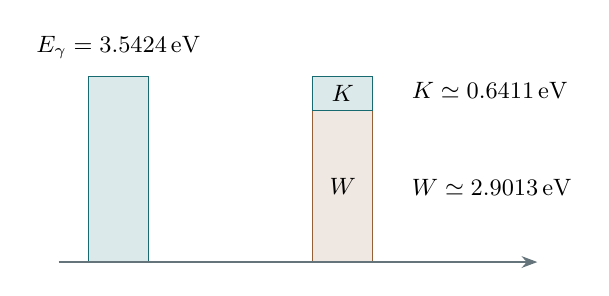
\begin{tikzpicture}[scale=.95,transform shape]
\filldraw[fill=accent!15,draw=accent] (0,0) rectangle (.8,2.4796800);
\filldraw[fill=warm!15,draw=warm] (3,0) rectangle (3.8,2.0309159);
\filldraw[fill=accent!15,draw=accent] (3,2.0309159) rectangle (3.8,2.4796800);
\node[above] at (.4,2.5996799999999998) {$E_\gamma=3.5424\,\mathrm{eV}$};
\node at (3.4,1.0154579745493106) {$W$};\node at (3.4,2.2552979745493102) {$K$};
\node[right] at (4.2,1) {$W\simeq2.9013\,\mathrm{eV}$};\node[right] at (4.2,2.3) {$K\simeq0.6411\,\mathrm{eV}$};
\draw[axis] (-.4,0)--(6,0);
\end{tikzpicture}
\figcaption{解图近1.8B\quad 同一光子能量分成逸出功与最大光电子动能}
\end{minipage}\end{center}
电子静能尺度给出动能近似的误差。记$u=p/(m_ec)$，当前值约$1.584\times10^{-3}$。相对论能量关系给
\[
K_{\rm rel}=\sqrt{m_e^2c^4+p^2c^2}-m_ec^2
=\frac{p^2}{2m_e}\left[1-\frac{p^2}{4m_e^2c^2}+\cdots\right].
\]
求展开时使用$\sqrt{1+u^2}=1+u^2/2-u^4/8+\cdots$，所以首个相对修正约$u^2/4=6.3\times10^{-7}$。解图近1.8C画这项误差随无量纲动量增长的关系；本题修正约百万分之零点六，远小于给定数据三位有效数字的量级，$W=2.90\,\mathrm{eV}$已与数据精度相符。
\begin{center}\begin{minipage}{.98\linewidth}\centering
\begin{tikzpicture}[scale=.88,transform shape]
\draw[axis] (0,0.0)--(7.3,0.0) node[right] {$u=p/(m_ec)$};
\draw[axis] (0,0)--(0,2.8);
\node[above left] at (0,2.8) {$(K_{\rm nr}-K_{\rm rel})/K_{\rm rel}$};
\draw[thin] (0.000000,0.0)--(0.000000,-0.06);\node[below,font=\scriptsize] at (0.000000,-0.08) {$ 0 $};
\draw[thin] (1.750000,0.0)--(1.750000,-0.06);\node[below,font=\scriptsize] at (1.750000,-0.08) {$ 0.05 $};
\draw[thin] (3.500000,0.0)--(3.500000,-0.06);\node[below,font=\scriptsize] at (3.500000,-0.08) {$ 0.1 $};
\draw[thin] (5.250000,0.0)--(5.250000,-0.06);\node[below,font=\scriptsize] at (5.250000,-0.08) {$ 0.15 $};
\draw[thin] (7.000000,0.0)--(7.000000,-0.06);\node[below,font=\scriptsize] at (7.000000,-0.08) {$ 0.2 $};
\draw[thin] (0,0.000000)--(-.06,0.000000);\node[left,font=\scriptsize] at (-.08,0.000000) {$ 0 $};
\draw[thin] (0,0.595238)--(-.06,0.595238);\node[left,font=\scriptsize] at (-.08,0.595238) {$ 0.0025 $};
\draw[thin] (0,1.190476)--(-.06,1.190476);\node[left,font=\scriptsize] at (-.08,1.190476) {$ 0.005 $};
\draw[thin] (0,2.380952)--(-.06,2.380952);\node[left,font=\scriptsize] at (-.08,2.380952) {$ 0.01 $};
\draw[thick,color=accent] plot coordinates {(0.0000000,0.0000000) (0.0291667,0.0000413) (0.0583333,0.0001653) (0.0875000,0.0003720) (0.1166667,0.0006614) (0.1458333,0.0010334) (0.1750000,0.0014881) (0.2041667,0.0020254) (0.2333333,0.0026455) (0.2625000,0.0033482) (0.2916667,0.0041335) (0.3208333,0.0050015) (0.3500000,0.0059522) (0.3791667,0.0069856) (0.4083333,0.0081016) (0.4375000,0.0093002) (0.4666667,0.0105815) (0.4958333,0.0119455) (0.5250000,0.0133921) (0.5541667,0.0149214) (0.5833333,0.0165332) (0.6125000,0.0182278) (0.6416667,0.0200049) (0.6708333,0.0218647) (0.7000000,0.0238071) (0.7291667,0.0258322) (0.7583333,0.0279398) (0.7875000,0.0301301) (0.8166667,0.0324030) (0.8458333,0.0347585) (0.8750000,0.0371966) (0.9041667,0.0397173) (0.9333333,0.0423205) (0.9625000,0.0450064) (0.9916667,0.0477748) (1.0208333,0.0506258) (1.0500000,0.0535594) (1.0791667,0.0565755) (1.1083333,0.0596742) (1.1375000,0.0628554) (1.1666667,0.0661192) (1.1958333,0.0694655) (1.2250000,0.0728943) (1.2541667,0.0764057) (1.2833333,0.0799996) (1.3125000,0.0836760) (1.3416667,0.0874348) (1.3708333,0.0912762) (1.4000000,0.0952000) (1.4291667,0.0992063) (1.4583333,0.1032951) (1.4875000,0.1074664) (1.5166667,0.1117201) (1.5458333,0.1160562) (1.5750000,0.1204748) (1.6041667,0.1249757) (1.6333333,0.1295591) (1.6625000,0.1342249) (1.6916667,0.1389731) (1.7208333,0.1438037) (1.7500000,0.1487166) (1.7791667,0.1537119) (1.8083333,0.1587896) (1.8375000,0.1639496) (1.8666667,0.1691919) (1.8958333,0.1745166) (1.9250000,0.1799236) (1.9541667,0.1854128) (1.9833333,0.1909844) (2.0125000,0.1966382) (2.0416667,0.2023743) (2.0708333,0.2081926) (2.1000000,0.2140932) (2.1291667,0.2200760) (2.1583333,0.2261410) (2.1875000,0.2322883) (2.2166667,0.2385177) (2.2458333,0.2448293) (2.2750000,0.2512230) (2.3041667,0.2576989) (2.3333333,0.2642570) (2.3625000,0.2708971) (2.3916667,0.2776194) (2.4208333,0.2844238) (2.4500000,0.2913102) (2.4791667,0.2982788) (2.5083333,0.3053294) (2.5375000,0.3124620) (2.5666667,0.3196766) (2.5958333,0.3269733) (2.6250000,0.3343519) (2.6541667,0.3418125) (2.6833333,0.3493551) (2.7125000,0.3569797) (2.7416667,0.3646861) (2.7708333,0.3724745) (2.8000000,0.3803448) (2.8291667,0.3882970) (2.8583333,0.3963310) (2.8875000,0.4044469) (2.9166667,0.4126446) (2.9458333,0.4209242) (2.9750000,0.4292855) (3.0041667,0.4377287) (3.0333333,0.4462535) (3.0625000,0.4548602) (3.0916667,0.4635486) (3.1208333,0.4723187) (3.1500000,0.4811705) (3.1791667,0.4901039) (3.2083333,0.4991190) (3.2375000,0.5082158) (3.2666667,0.5173942) (3.2958333,0.5266542) (3.3250000,0.5359958) (3.3541667,0.5454189) (3.3833333,0.5549236) (3.4125000,0.5645098) (3.4416667,0.5741775) (3.4708333,0.5839267) (3.5000000,0.5937574) (3.5291667,0.6036695) (3.5583333,0.6136631) (3.5875000,0.6237380) (3.6166667,0.6338944) (3.6458333,0.6441321) (3.6750000,0.6544511) (3.7041667,0.6648515) (3.7333333,0.6753332) (3.7625000,0.6858961) (3.7916667,0.6965403) (3.8208333,0.7072658) (3.8500000,0.7180725) (3.8791667,0.7289603) (3.9083333,0.7399294) (3.9375000,0.7509795) (3.9666667,0.7621109) (3.9958333,0.7733233) (4.0250000,0.7846168) (4.0541667,0.7959913) (4.0833333,0.8074469) (4.1125000,0.8189835) (4.1416667,0.8306011) (4.1708333,0.8422997) (4.2000000,0.8540792) (4.2291667,0.8659396) (4.2583333,0.8778809) (4.2875000,0.8899031) (4.3166667,0.9020061) (4.3458333,0.9141899) (4.3750000,0.9264546) (4.4041667,0.9388000) (4.4333333,0.9512262) (4.4625000,0.9637330) (4.4916667,0.9763206) (4.5208333,0.9889889) (4.5500000,1.0017378) (4.5791667,1.0145673) (4.6083333,1.0274774) (4.6375000,1.0404681) (4.6666667,1.0535393) (4.6958333,1.0666910) (4.7250000,1.0799232) (4.7541667,1.0932359) (4.7833333,1.1066290) (4.8125000,1.1201026) (4.8416667,1.1336565) (4.8708333,1.1472908) (4.9000000,1.1610053) (4.9291667,1.1748002) (4.9583333,1.1886754) (4.9875000,1.2026308) (5.0166667,1.2166664) (5.0458333,1.2307822) (5.0750000,1.2449782) (5.1041667,1.2592543) (5.1333333,1.2736105) (5.1625000,1.2880468) (5.1916667,1.3025631) (5.2208333,1.3171595) (5.2500000,1.3318358) (5.2791667,1.3465921) (5.3083333,1.3614283) (5.3375000,1.3763444) (5.3666667,1.3913404) (5.3958333,1.4064162) (5.4250000,1.4215719) (5.4541667,1.4368073) (5.4833333,1.4521225) (5.5125000,1.4675173) (5.5416667,1.4829919) (5.5708333,1.4985462) (5.6000000,1.5141800) (5.6291667,1.5298935) (5.6583333,1.5456865) (5.6875000,1.5615590) (5.7166667,1.5775111) (5.7458333,1.5935426) (5.7750000,1.6096536) (5.8041667,1.6258439) (5.8333333,1.6421137) (5.8625000,1.6584628) (5.8916667,1.6748912) (5.9208333,1.6913989) (5.9500000,1.7079858) (5.9791667,1.7246519) (6.0083333,1.7413972) (6.0375000,1.7582217) (6.0666667,1.7751253) (6.0958333,1.7921080) (6.1250000,1.8091697) (6.1541667,1.8263104) (6.1833333,1.8435301) (6.2125000,1.8608288) (6.2416667,1.8782063) (6.2708333,1.8956628) (6.3000000,1.9131981) (6.3291667,1.9308122) (6.3583333,1.9485050) (6.3875000,1.9662767) (6.4166667,1.9841270) (6.4458333,2.0020560) (6.4750000,2.0200636) (6.5041667,2.0381499) (6.5333333,2.0563147) (6.5625000,2.0745580) (6.5916667,2.0928798) (6.6208333,2.1112801) (6.6500000,2.1297589) (6.6791667,2.1483160) (6.7083333,2.1669514) (6.7375000,2.1856652) (6.7666667,2.2044573) (6.7958333,2.2233276) (6.8250000,2.2422761) (6.8541667,2.2613028) (6.8833333,2.2804076) (6.9125000,2.2995905) (6.9416667,2.3188515) (6.9708333,2.3381905) (7.0000000,2.3576075)};
\end{tikzpicture}
\figcaption{解图近1.8C\quad 电子动量相对静能尺度给出的非相对论近似误差}
\end{minipage}\end{center}
同一材料在没有额外电势的条件下，改变照射频率会使$K_{\max}=h\nu-W$变化。结合轨道动量，得到$r^2=2m_e(h\nu-W)/(e^2B^2)$，直线的零点为阈频$\nu_{\rm th}=W/h$。解图近1.8D显示该直线关系；更高的入射单光子能量给更大的最大轨道半径，直线截距则给材料的逸出条件。
\begin{center}\begin{minipage}{.98\linewidth}\centering
\begin{tikzpicture}[scale=.88,transform shape]
\draw[axis] (0,0.0)--(7.3,0.0) node[right] {$\nu/\nu_{\rm th}$};
\draw[axis] (0,0)--(0,2.8);
\node[above left] at (0,2.8) {$e^2B^2r^2/(2m_eW)$};
\draw[thin] (0.000000,0.0)--(0.000000,-0.06);\node[below,font=\scriptsize] at (0.000000,-0.08) {$ 1 $};
\draw[thin] (2.333333,0.0)--(2.333333,-0.06);\node[below,font=\scriptsize] at (2.333333,-0.08) {$ 1.2 $};
\draw[thin] (4.666667,0.0)--(4.666667,-0.06);\node[below,font=\scriptsize] at (4.666667,-0.08) {$ 1.4 $};
\draw[thin] (7.000000,0.0)--(7.000000,-0.06);\node[below,font=\scriptsize] at (7.000000,-0.08) {$ 1.6 $};
\draw[thin] (0,0.000000)--(-.06,0.000000);\node[left,font=\scriptsize] at (-.08,0.000000) {$ 0 $};
\draw[thin] (0,0.769231)--(-.06,0.769231);\node[left,font=\scriptsize] at (-.08,0.769231) {$ 0.2 $};
\draw[thin] (0,1.538462)--(-.06,1.538462);\node[left,font=\scriptsize] at (-.08,1.538462) {$ 0.4 $};
\draw[thin] (0,2.307692)--(-.06,2.307692);\node[left,font=\scriptsize] at (-.08,2.307692) {$ 0.6 $};
\draw[thick,color=accent] plot coordinates {(0.0000000,0.0000000) (0.0291667,0.0096154) (0.0583333,0.0192308) (0.0875000,0.0288462) (0.1166667,0.0384615) (0.1458333,0.0480769) (0.1750000,0.0576923) (0.2041667,0.0673077) (0.2333333,0.0769231) (0.2625000,0.0865385) (0.2916667,0.0961538) (0.3208333,0.1057692) (0.3500000,0.1153846) (0.3791667,0.1250000) (0.4083333,0.1346154) (0.4375000,0.1442308) (0.4666667,0.1538462) (0.4958333,0.1634615) (0.5250000,0.1730769) (0.5541667,0.1826923) (0.5833333,0.1923077) (0.6125000,0.2019231) (0.6416667,0.2115385) (0.6708333,0.2211538) (0.7000000,0.2307692) (0.7291667,0.2403846) (0.7583333,0.2500000) (0.7875000,0.2596154) (0.8166667,0.2692308) (0.8458333,0.2788462) (0.8750000,0.2884615) (0.9041667,0.2980769) (0.9333333,0.3076923) (0.9625000,0.3173077) (0.9916667,0.3269231) (1.0208333,0.3365385) (1.0500000,0.3461538) (1.0791667,0.3557692) (1.1083333,0.3653846) (1.1375000,0.3750000) (1.1666667,0.3846154) (1.1958333,0.3942308) (1.2250000,0.4038462) (1.2541667,0.4134615) (1.2833333,0.4230769) (1.3125000,0.4326923) (1.3416667,0.4423077) (1.3708333,0.4519231) (1.4000000,0.4615385) (1.4291667,0.4711538) (1.4583333,0.4807692) (1.4875000,0.4903846) (1.5166667,0.5000000) (1.5458333,0.5096154) (1.5750000,0.5192308) (1.6041667,0.5288462) (1.6333333,0.5384615) (1.6625000,0.5480769) (1.6916667,0.5576923) (1.7208333,0.5673077) (1.7500000,0.5769231) (1.7791667,0.5865385) (1.8083333,0.5961538) (1.8375000,0.6057692) (1.8666667,0.6153846) (1.8958333,0.6250000) (1.9250000,0.6346154) (1.9541667,0.6442308) (1.9833333,0.6538462) (2.0125000,0.6634615) (2.0416667,0.6730769) (2.0708333,0.6826923) (2.1000000,0.6923077) (2.1291667,0.7019231) (2.1583333,0.7115385) (2.1875000,0.7211538) (2.2166667,0.7307692) (2.2458333,0.7403846) (2.2750000,0.7500000) (2.3041667,0.7596154) (2.3333333,0.7692308) (2.3625000,0.7788462) (2.3916667,0.7884615) (2.4208333,0.7980769) (2.4500000,0.8076923) (2.4791667,0.8173077) (2.5083333,0.8269231) (2.5375000,0.8365385) (2.5666667,0.8461538) (2.5958333,0.8557692) (2.6250000,0.8653846) (2.6541667,0.8750000) (2.6833333,0.8846154) (2.7125000,0.8942308) (2.7416667,0.9038462) (2.7708333,0.9134615) (2.8000000,0.9230769) (2.8291667,0.9326923) (2.8583333,0.9423077) (2.8875000,0.9519231) (2.9166667,0.9615385) (2.9458333,0.9711538) (2.9750000,0.9807692) (3.0041667,0.9903846) (3.0333333,1.0000000) (3.0625000,1.0096154) (3.0916667,1.0192308) (3.1208333,1.0288462) (3.1500000,1.0384615) (3.1791667,1.0480769) (3.2083333,1.0576923) (3.2375000,1.0673077) (3.2666667,1.0769231) (3.2958333,1.0865385) (3.3250000,1.0961538) (3.3541667,1.1057692) (3.3833333,1.1153846) (3.4125000,1.1250000) (3.4416667,1.1346154) (3.4708333,1.1442308) (3.5000000,1.1538462) (3.5291667,1.1634615) (3.5583333,1.1730769) (3.5875000,1.1826923) (3.6166667,1.1923077) (3.6458333,1.2019231) (3.6750000,1.2115385) (3.7041667,1.2211538) (3.7333333,1.2307692) (3.7625000,1.2403846) (3.7916667,1.2500000) (3.8208333,1.2596154) (3.8500000,1.2692308) (3.8791667,1.2788462) (3.9083333,1.2884615) (3.9375000,1.2980769) (3.9666667,1.3076923) (3.9958333,1.3173077) (4.0250000,1.3269231) (4.0541667,1.3365385) (4.0833333,1.3461538) (4.1125000,1.3557692) (4.1416667,1.3653846) (4.1708333,1.3750000) (4.2000000,1.3846154) (4.2291667,1.3942308) (4.2583333,1.4038462) (4.2875000,1.4134615) (4.3166667,1.4230769) (4.3458333,1.4326923) (4.3750000,1.4423077) (4.4041667,1.4519231) (4.4333333,1.4615385) (4.4625000,1.4711538) (4.4916667,1.4807692) (4.5208333,1.4903846) (4.5500000,1.5000000) (4.5791667,1.5096154) (4.6083333,1.5192308) (4.6375000,1.5288462) (4.6666667,1.5384615) (4.6958333,1.5480769) (4.7250000,1.5576923) (4.7541667,1.5673077) (4.7833333,1.5769231) (4.8125000,1.5865385) (4.8416667,1.5961538) (4.8708333,1.6057692) (4.9000000,1.6153846) (4.9291667,1.6250000) (4.9583333,1.6346154) (4.9875000,1.6442308) (5.0166667,1.6538462) (5.0458333,1.6634615) (5.0750000,1.6730769) (5.1041667,1.6826923) (5.1333333,1.6923077) (5.1625000,1.7019231) (5.1916667,1.7115385) (5.2208333,1.7211538) (5.2500000,1.7307692) (5.2791667,1.7403846) (5.3083333,1.7500000) (5.3375000,1.7596154) (5.3666667,1.7692308) (5.3958333,1.7788462) (5.4250000,1.7884615) (5.4541667,1.7980769) (5.4833333,1.8076923) (5.5125000,1.8173077) (5.5416667,1.8269231) (5.5708333,1.8365385) (5.6000000,1.8461538) (5.6291667,1.8557692) (5.6583333,1.8653846) (5.6875000,1.8750000) (5.7166667,1.8846154) (5.7458333,1.8942308) (5.7750000,1.9038462) (5.8041667,1.9134615) (5.8333333,1.9230769) (5.8625000,1.9326923) (5.8916667,1.9423077) (5.9208333,1.9519231) (5.9500000,1.9615385) (5.9791667,1.9711538) (6.0083333,1.9807692) (6.0375000,1.9903846) (6.0666667,2.0000000) (6.0958333,2.0096154) (6.1250000,2.0192308) (6.1541667,2.0288462) (6.1833333,2.0384615) (6.2125000,2.0480769) (6.2416667,2.0576923) (6.2708333,2.0673077) (6.3000000,2.0769231) (6.3291667,2.0865385) (6.3583333,2.0961538) (6.3875000,2.1057692) (6.4166667,2.1153846) (6.4458333,2.1250000) (6.4750000,2.1346154) (6.5041667,2.1442308) (6.5333333,2.1538462) (6.5625000,2.1634615) (6.5916667,2.1730769) (6.6208333,2.1826923) (6.6500000,2.1923077) (6.6791667,2.2019231) (6.7083333,2.2115385) (6.7375000,2.2211538) (6.7666667,2.2307692) (6.7958333,2.2403846) (6.8250000,2.2500000) (6.8541667,2.2596154) (6.8833333,2.2692308) (6.9125000,2.2788462) (6.9416667,2.2884615) (6.9708333,2.2980769) (7.0000000,2.3076923)};
\end{tikzpicture}
\figcaption{解图近1.8D\quad 最高光电子半径平方随频率线性增加}
\end{minipage}\end{center}


\Needspace{13\baselineskip}

\pdfbookmark[2]{第 9 题 自由电子为何不能完整吸收单光子}{q9}

\section*{第 9 题\quad 自由电子为何不能完整吸收单光子}\label{q:9}

证明孤立、起初静止的自由电子不可能完整吸收一个非零能量光子后仍成为同一种自由电子。要求同时使用能量和动量守恒，并解释束缚电子产生光电效应为何不矛盾。

\begin{center}\begin{minipage}{.98\linewidth}\centering
\begin{tikzpicture}[scale=.9,transform shape]
\draw[traj] plot coordinates {(-2.00000,0.00000) (-1.98561,0.01432) (-1.97122,0.02714) (-1.95683,0.03715) (-1.94245,0.04330) (-1.92806,0.04495) (-1.91367,0.04193) (-1.89928,0.03455) (-1.88489,0.02358) (-1.87050,0.01017) (-1.85612,-0.00431) (-1.84173,-0.01833) (-1.82734,-0.03045) (-1.81295,-0.03941) (-1.79856,-0.04427) (-1.78417,-0.04454) (-1.76978,-0.04017) (-1.75540,-0.03163) (-1.74101,-0.01981) (-1.72662,-0.00593) (-1.71223,0.00857) (-1.69784,0.02218) (-1.68345,0.03348) (-1.66906,0.04131) (-1.65468,0.04484) (-1.64029,0.04372) (-1.62590,0.03805) (-1.61151,0.02843) (-1.59712,0.01585) (-1.58273,0.00163) (-1.56835,-0.01276) (-1.55396,-0.02582) (-1.53957,-0.03621) (-1.52518,-0.04283) (-1.51079,-0.04500) (-1.49640,-0.04249) (-1.48201,-0.03557) (-1.46763,-0.02496) (-1.45324,-0.01175) (-1.43885,0.00268) (-1.42446,0.01683) (-1.41007,0.02923) (-1.39568,0.03860) (-1.38129,0.04395) (-1.36691,0.04474) (-1.35252,0.04088) (-1.33813,0.03277) (-1.32374,0.02126) (-1.30935,0.00754) (-1.29496,-0.00696) (-1.28058,-0.02074) (-1.26619,-0.03237) (-1.25180,-0.04063) (-1.23741,-0.04467) (-1.22302,-0.04407) (-1.20863,-0.03889) (-1.19424,-0.02967) (-1.17986,-0.01737) (-1.16547,-0.00326) (-1.15108,0.01118) (-1.13669,0.02447) (-1.12230,0.03521) (-1.10791,0.04230) (-1.09353,0.04499) (-1.07914,0.04300) (-1.06475,0.03655) (-1.05036,0.02630) (-1.03597,0.01332) (-1.02158,-0.00105) (-1.00719,-0.01530) (-0.99281,-0.02797) (-0.97842,-0.03773) (-0.96403,-0.04357) (-0.94964,-0.04489) (-0.93525,-0.04154) (-0.92086,-0.03387) (-0.90647,-0.02269) (-0.89209,-0.00915) (-0.87770,0.00534) (-0.86331,0.01928) (-0.84892,0.03121) (-0.83453,0.03990) (-0.82014,0.04445) (-0.80576,0.04437) (-0.79137,0.03969) (-0.77698,0.03088) (-0.76259,0.01887) (-0.74820,0.00489) (-0.73381,-0.00960) (-0.71942,-0.02308) (-0.70504,-0.03417) (-0.69065,-0.04171) (-0.67626,-0.04492) (-0.66187,-0.04346) (-0.64748,-0.03748) (-0.63309,-0.02761) (-0.61871,-0.01487) (-0.60432,-0.00059) (-0.58993,0.01376) (-0.57554,0.02667) (-0.56115,0.03682) (-0.54676,0.04314) (-0.53237,0.04497) (-0.51799,0.04214) (-0.50360,0.03492) (-0.48921,0.02408) (-0.47482,0.01074) (-0.46043,-0.00372) (-0.44604,-0.01779) (-0.43165,-0.03002) (-0.41727,-0.03912) (-0.40288,-0.04416) (-0.38849,-0.04462) (-0.37410,-0.04043) (-0.35971,-0.03205) (-0.34532,-0.02034) (-0.33094,-0.00651) (-0.31655,0.00799) (-0.30216,0.02167) (-0.28777,0.03309) (-0.27338,0.04107) (-0.25899,0.04479) (-0.24460,0.04385) (-0.23022,0.03836) (-0.21583,0.02888) (-0.20144,0.01640) (-0.18705,0.00222) (-0.17266,-0.01219) (-0.15827,-0.02534) (-0.14388,-0.03585) (-0.12950,-0.04264) (-0.11511,-0.04500) (-0.10072,-0.04268) (-0.08633,-0.03593) (-0.07194,-0.02545) (-0.05755,-0.01232) (-0.04317,0.00209) (-0.02878,0.01628) (-0.01439,0.02878) (0.00000,0.03829)};\draw[motion] (-0.18000,0.00000)--(0.00000,0.00000);\node[above] at (-1.00000,0.00000) {$E_\gamma,\ E_\gamma/c$};\fill (0.00000,0.00000) circle(.035);\node[below] at (0.00000,0.00000) {$e^-$};\node[above] at (0.00000,0.50000) {初始静止};\draw[force] (0.70000,0.00000)--(4.00000,0.00000);\node[above] at (3.00000,0.20000) {假设：只剩一个电子};
\end{tikzpicture}
\figcaption{图近1.9\quad 假定末态只有一个同质量自由电子。}
\end{minipage}\end{center}

\Needspace{6\baselineskip}\subsection*{解答}


图近1.9中的系统只含一个起初静止的自由电子和一个入射光子。电子的不变质量固定为$m_e$，光子的能量$E_\gamma=h\nu>0$、动量大小$E_\gamma/c$。所谓完整吸收，是在相互作用后只留下同一种自由电子；这个设定同时规定了末态的粒子数和不变质量。选入射方向为$x$轴，分别写总能量与总动量守恒：
\[
 E_f=m_ec^2+E_\gamma,\qquad p_f=\frac{E_\gamma}{c}.
\]
初电子虽然动量为零，能量仍为$m_ec^2$，这项与光子能量一起进入左端。自由电子的末能量与末动量还满足
\[
E_f^2=m_e^2c^4+p_f^2c^2.
\]
把两个守恒关系代入上式，得到
\[
(m_ec^2+E_\gamma)^2=m_e^2c^4+E_\gamma^2
\quad\Longrightarrow\quad 2m_ec^2E_\gamma=0,
\]
左端由两个正量相乘，所设单电子末态与守恒式互不相容。只有$E_\gamma=0$的退化情况给出恒等式，它对应初、末均静止的电子。
\begin{center}\begin{minipage}{.98\linewidth}\centering
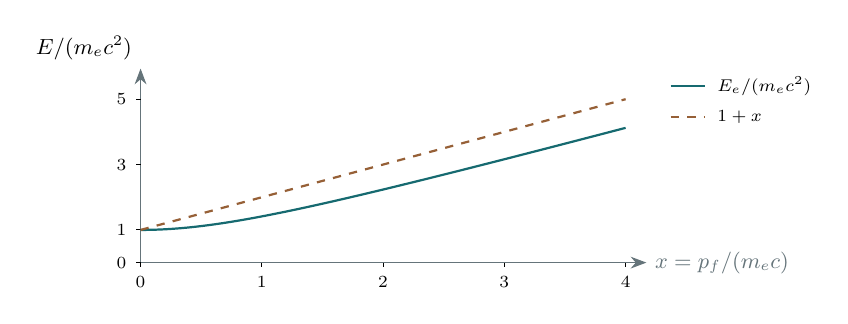
\begin{tikzpicture}[scale=.88,transform shape]
\draw[axis] (0,0.0)--(7.3,0.0) node[right] {$x=p_f/(m_ec)$};
\draw[axis] (0,0)--(0,2.8);
\node[above left] at (0,2.8) {$E/(m_ec^2)$};
\draw[thin] (0.000000,0.0)--(0.000000,-0.06);\node[below,font=\scriptsize] at (0.000000,-0.08) {$ 0 $};
\draw[thin] (1.750000,0.0)--(1.750000,-0.06);\node[below,font=\scriptsize] at (1.750000,-0.08) {$ 1 $};
\draw[thin] (3.500000,0.0)--(3.500000,-0.06);\node[below,font=\scriptsize] at (3.500000,-0.08) {$ 2 $};
\draw[thin] (5.250000,0.0)--(5.250000,-0.06);\node[below,font=\scriptsize] at (5.250000,-0.08) {$ 3 $};
\draw[thin] (7.000000,0.0)--(7.000000,-0.06);\node[below,font=\scriptsize] at (7.000000,-0.08) {$ 4 $};
\draw[thin] (0,0.000000)--(-.06,0.000000);\node[left,font=\scriptsize] at (-.08,0.000000) {$ 0 $};
\draw[thin] (0,0.471698)--(-.06,0.471698);\node[left,font=\scriptsize] at (-.08,0.471698) {$ 1 $};
\draw[thin] (0,1.415094)--(-.06,1.415094);\node[left,font=\scriptsize] at (-.08,1.415094) {$ 3 $};
\draw[thin] (0,2.358491)--(-.06,2.358491);\node[left,font=\scriptsize] at (-.08,2.358491) {$ 5 $};
\draw[thick,color=accent] plot coordinates {(0.0000000,0.4716981) (0.0291667,0.4717636) (0.0583333,0.4719601) (0.0875000,0.4722874) (0.1166667,0.4727452) (0.1458333,0.4733331) (0.1750000,0.4740507) (0.2041667,0.4748974) (0.2333333,0.4758725) (0.2625000,0.4769752) (0.2916667,0.4782046) (0.3208333,0.4795597) (0.3500000,0.4810396) (0.3791667,0.4826429) (0.4083333,0.4843686) (0.4375000,0.4862153) (0.4666667,0.4881816) (0.4958333,0.4902661) (0.5250000,0.4924673) (0.5541667,0.4947836) (0.5833333,0.4972135) (0.6125000,0.4997552) (0.6416667,0.5024071) (0.6708333,0.5051674) (0.7000000,0.5080344) (0.7291667,0.5110063) (0.7583333,0.5140812) (0.7875000,0.5172574) (0.8166667,0.5205329) (0.8458333,0.5239059) (0.8750000,0.5273745) (0.9041667,0.5309369) (0.9333333,0.5345912) (0.9625000,0.5383355) (0.9916667,0.5421679) (1.0208333,0.5460866) (1.0500000,0.5500898) (1.0791667,0.5541756) (1.1083333,0.5583422) (1.1375000,0.5625878) (1.1666667,0.5669106) (1.1958333,0.5713089) (1.2250000,0.5757809) (1.2541667,0.5803250) (1.2833333,0.5849395) (1.3125000,0.5896226) (1.3416667,0.5943729) (1.3708333,0.5991886) (1.4000000,0.6040683) (1.4291667,0.6090104) (1.4583333,0.6140133) (1.4875000,0.6190757) (1.5166667,0.6241960) (1.5458333,0.6293729) (1.5750000,0.6346049) (1.6041667,0.6398907) (1.6333333,0.6452291) (1.6625000,0.6506186) (1.6916667,0.6560581) (1.7208333,0.6615462) (1.7500000,0.6670819) (1.7791667,0.6726639) (1.8083333,0.6782910) (1.8375000,0.6839623) (1.8666667,0.6896765) (1.8958333,0.6954326) (1.9250000,0.7012297) (1.9541667,0.7070666) (1.9833333,0.7129424) (2.0125000,0.7188562) (2.0416667,0.7248070) (2.0708333,0.7307939) (2.1000000,0.7368160) (2.1291667,0.7428725) (2.1583333,0.7489626) (2.1875000,0.7550854) (2.2166667,0.7612402) (2.2458333,0.7674261) (2.2750000,0.7736424) (2.3041667,0.7798885) (2.3333333,0.7861635) (2.3625000,0.7924669) (2.3916667,0.7987978) (2.4208333,0.8051558) (2.4500000,0.8115401) (2.4791667,0.8179502) (2.5083333,0.8243853) (2.5375000,0.8308450) (2.5666667,0.8373287) (2.5958333,0.8438359) (2.6250000,0.8503659) (2.6541667,0.8569182) (2.6833333,0.8634925) (2.7125000,0.8700881) (2.7416667,0.8767045) (2.7708333,0.8833414) (2.8000000,0.8899982) (2.8291667,0.8966746) (2.8583333,0.9033700) (2.8875000,0.9100840) (2.9166667,0.9168163) (2.9458333,0.9235665) (2.9750000,0.9303341) (3.0041667,0.9371188) (3.0333333,0.9439202) (3.0625000,0.9507379) (3.0916667,0.9575717) (3.1208333,0.9644211) (3.1500000,0.9712859) (3.1791667,0.9781656) (3.2083333,0.9850601) (3.2375000,0.9919689) (3.2666667,0.9988918) (3.2958333,1.0058286) (3.3250000,1.0127788) (3.3541667,1.0197423) (3.3833333,1.0267187) (3.4125000,1.0337079) (3.4416667,1.0407095) (3.4708333,1.0477233) (3.5000000,1.0547490) (3.5291667,1.0617865) (3.5583333,1.0688355) (3.5875000,1.0758957) (3.6166667,1.0829670) (3.6458333,1.0900491) (3.6750000,1.0971418) (3.7041667,1.1042450) (3.7333333,1.1113583) (3.7625000,1.1184817) (3.7916667,1.1256149) (3.8208333,1.1327577) (3.8500000,1.1399100) (3.8791667,1.1470716) (3.9083333,1.1542423) (3.9375000,1.1614219) (3.9666667,1.1686103) (3.9958333,1.1758074) (4.0250000,1.1830128) (4.0541667,1.1902266) (4.0833333,1.1974486) (4.1125000,1.2046786) (4.1416667,1.2119164) (4.1708333,1.2191619) (4.2000000,1.2264151) (4.2291667,1.2336757) (4.2583333,1.2409436) (4.2875000,1.2482187) (4.3166667,1.2555009) (4.3458333,1.2627901) (4.3750000,1.2700860) (4.4041667,1.2773887) (4.4333333,1.2846980) (4.4625000,1.2920138) (4.4916667,1.2993359) (4.5208333,1.3066643) (4.5500000,1.3139989) (4.5791667,1.3213395) (4.6083333,1.3286861) (4.6375000,1.3360386) (4.6666667,1.3433968) (4.6958333,1.3507607) (4.7250000,1.3581302) (4.7541667,1.3655052) (4.7833333,1.3728855) (4.8125000,1.3802712) (4.8416667,1.3876621) (4.8708333,1.3950582) (4.9000000,1.4024593) (4.9291667,1.4098654) (4.9583333,1.4172764) (4.9875000,1.4246923) (5.0166667,1.4321129) (5.0458333,1.4395382) (5.0750000,1.4469681) (5.1041667,1.4544025) (5.1333333,1.4618414) (5.1625000,1.4692847) (5.1916667,1.4767324) (5.2208333,1.4841843) (5.2500000,1.4916404) (5.2791667,1.4991007) (5.3083333,1.5065650) (5.3375000,1.5140334) (5.3666667,1.5215057) (5.3958333,1.5289819) (5.4250000,1.5364620) (5.4541667,1.5439459) (5.4833333,1.5514335) (5.5125000,1.5589248) (5.5416667,1.5664197) (5.5708333,1.5739182) (5.6000000,1.5814202) (5.6291667,1.5889258) (5.6583333,1.5964347) (5.6875000,1.6039470) (5.7166667,1.6114626) (5.7458333,1.6189816) (5.7750000,1.6265037) (5.8041667,1.6340291) (5.8333333,1.6415576) (5.8625000,1.6490893) (5.8916667,1.6566239) (5.9208333,1.6641617) (5.9500000,1.6717024) (5.9791667,1.6792460) (6.0083333,1.6867926) (6.0375000,1.6943420) (6.0666667,1.7018942) (6.0958333,1.7094493) (6.1250000,1.7170070) (6.1541667,1.7245676) (6.1833333,1.7321307) (6.2125000,1.7396966) (6.2416667,1.7472650) (6.2708333,1.7548360) (6.3000000,1.7624096) (6.3291667,1.7699857) (6.3583333,1.7775642) (6.3875000,1.7851452) (6.4166667,1.7927287) (6.4458333,1.8003145) (6.4750000,1.8079026) (6.5041667,1.8154931) (6.5333333,1.8230859) (6.5625000,1.8306810) (6.5916667,1.8382783) (6.6208333,1.8458778) (6.6500000,1.8534795) (6.6791667,1.8610834) (6.7083333,1.8686894) (6.7375000,1.8762975) (6.7666667,1.8839076) (6.7958333,1.8915199) (6.8250000,1.8991342) (6.8541667,1.9067504) (6.8833333,1.9143687) (6.9125000,1.9219889) (6.9416667,1.9296111) (6.9708333,1.9372352) (7.0000000,1.9448611)};
\draw[thick,color=accent] (7.65,2.55)--(8.15,2.55);\node[right,font=\scriptsize] at (8.2,2.55) {$E_e/(m_ec^2)$};
\draw[thick,dashed,color=warm] plot coordinates {(0.0000000,0.4716981) (0.0291667,0.4795597) (0.0583333,0.4874214) (0.0875000,0.4952830) (0.1166667,0.5031447) (0.1458333,0.5110063) (0.1750000,0.5188679) (0.2041667,0.5267296) (0.2333333,0.5345912) (0.2625000,0.5424528) (0.2916667,0.5503145) (0.3208333,0.5581761) (0.3500000,0.5660377) (0.3791667,0.5738994) (0.4083333,0.5817610) (0.4375000,0.5896226) (0.4666667,0.5974843) (0.4958333,0.6053459) (0.5250000,0.6132075) (0.5541667,0.6210692) (0.5833333,0.6289308) (0.6125000,0.6367925) (0.6416667,0.6446541) (0.6708333,0.6525157) (0.7000000,0.6603774) (0.7291667,0.6682390) (0.7583333,0.6761006) (0.7875000,0.6839623) (0.8166667,0.6918239) (0.8458333,0.6996855) (0.8750000,0.7075472) (0.9041667,0.7154088) (0.9333333,0.7232704) (0.9625000,0.7311321) (0.9916667,0.7389937) (1.0208333,0.7468553) (1.0500000,0.7547170) (1.0791667,0.7625786) (1.1083333,0.7704403) (1.1375000,0.7783019) (1.1666667,0.7861635) (1.1958333,0.7940252) (1.2250000,0.8018868) (1.2541667,0.8097484) (1.2833333,0.8176101) (1.3125000,0.8254717) (1.3416667,0.8333333) (1.3708333,0.8411950) (1.4000000,0.8490566) (1.4291667,0.8569182) (1.4583333,0.8647799) (1.4875000,0.8726415) (1.5166667,0.8805031) (1.5458333,0.8883648) (1.5750000,0.8962264) (1.6041667,0.9040881) (1.6333333,0.9119497) (1.6625000,0.9198113) (1.6916667,0.9276730) (1.7208333,0.9355346) (1.7500000,0.9433962) (1.7791667,0.9512579) (1.8083333,0.9591195) (1.8375000,0.9669811) (1.8666667,0.9748428) (1.8958333,0.9827044) (1.9250000,0.9905660) (1.9541667,0.9984277) (1.9833333,1.0062893) (2.0125000,1.0141509) (2.0416667,1.0220126) (2.0708333,1.0298742) (2.1000000,1.0377358) (2.1291667,1.0455975) (2.1583333,1.0534591) (2.1875000,1.0613208) (2.2166667,1.0691824) (2.2458333,1.0770440) (2.2750000,1.0849057) (2.3041667,1.0927673) (2.3333333,1.1006289) (2.3625000,1.1084906) (2.3916667,1.1163522) (2.4208333,1.1242138) (2.4500000,1.1320755) (2.4791667,1.1399371) (2.5083333,1.1477987) (2.5375000,1.1556604) (2.5666667,1.1635220) (2.5958333,1.1713836) (2.6250000,1.1792453) (2.6541667,1.1871069) (2.6833333,1.1949686) (2.7125000,1.2028302) (2.7416667,1.2106918) (2.7708333,1.2185535) (2.8000000,1.2264151) (2.8291667,1.2342767) (2.8583333,1.2421384) (2.8875000,1.2500000) (2.9166667,1.2578616) (2.9458333,1.2657233) (2.9750000,1.2735849) (3.0041667,1.2814465) (3.0333333,1.2893082) (3.0625000,1.2971698) (3.0916667,1.3050314) (3.1208333,1.3128931) (3.1500000,1.3207547) (3.1791667,1.3286164) (3.2083333,1.3364780) (3.2375000,1.3443396) (3.2666667,1.3522013) (3.2958333,1.3600629) (3.3250000,1.3679245) (3.3541667,1.3757862) (3.3833333,1.3836478) (3.4125000,1.3915094) (3.4416667,1.3993711) (3.4708333,1.4072327) (3.5000000,1.4150943) (3.5291667,1.4229560) (3.5583333,1.4308176) (3.5875000,1.4386792) (3.6166667,1.4465409) (3.6458333,1.4544025) (3.6750000,1.4622642) (3.7041667,1.4701258) (3.7333333,1.4779874) (3.7625000,1.4858491) (3.7916667,1.4937107) (3.8208333,1.5015723) (3.8500000,1.5094340) (3.8791667,1.5172956) (3.9083333,1.5251572) (3.9375000,1.5330189) (3.9666667,1.5408805) (3.9958333,1.5487421) (4.0250000,1.5566038) (4.0541667,1.5644654) (4.0833333,1.5723270) (4.1125000,1.5801887) (4.1416667,1.5880503) (4.1708333,1.5959119) (4.2000000,1.6037736) (4.2291667,1.6116352) (4.2583333,1.6194969) (4.2875000,1.6273585) (4.3166667,1.6352201) (4.3458333,1.6430818) (4.3750000,1.6509434) (4.4041667,1.6588050) (4.4333333,1.6666667) (4.4625000,1.6745283) (4.4916667,1.6823899) (4.5208333,1.6902516) (4.5500000,1.6981132) (4.5791667,1.7059748) (4.6083333,1.7138365) (4.6375000,1.7216981) (4.6666667,1.7295597) (4.6958333,1.7374214) (4.7250000,1.7452830) (4.7541667,1.7531447) (4.7833333,1.7610063) (4.8125000,1.7688679) (4.8416667,1.7767296) (4.8708333,1.7845912) (4.9000000,1.7924528) (4.9291667,1.8003145) (4.9583333,1.8081761) (4.9875000,1.8160377) (5.0166667,1.8238994) (5.0458333,1.8317610) (5.0750000,1.8396226) (5.1041667,1.8474843) (5.1333333,1.8553459) (5.1625000,1.8632075) (5.1916667,1.8710692) (5.2208333,1.8789308) (5.2500000,1.8867925) (5.2791667,1.8946541) (5.3083333,1.9025157) (5.3375000,1.9103774) (5.3666667,1.9182390) (5.3958333,1.9261006) (5.4250000,1.9339623) (5.4541667,1.9418239) (5.4833333,1.9496855) (5.5125000,1.9575472) (5.5416667,1.9654088) (5.5708333,1.9732704) (5.6000000,1.9811321) (5.6291667,1.9889937) (5.6583333,1.9968553) (5.6875000,2.0047170) (5.7166667,2.0125786) (5.7458333,2.0204403) (5.7750000,2.0283019) (5.8041667,2.0361635) (5.8333333,2.0440252) (5.8625000,2.0518868) (5.8916667,2.0597484) (5.9208333,2.0676101) (5.9500000,2.0754717) (5.9791667,2.0833333) (6.0083333,2.0911950) (6.0375000,2.0990566) (6.0666667,2.1069182) (6.0958333,2.1147799) (6.1250000,2.1226415) (6.1541667,2.1305031) (6.1833333,2.1383648) (6.2125000,2.1462264) (6.2416667,2.1540881) (6.2708333,2.1619497) (6.3000000,2.1698113) (6.3291667,2.1776730) (6.3583333,2.1855346) (6.3875000,2.1933962) (6.4166667,2.2012579) (6.4458333,2.2091195) (6.4750000,2.2169811) (6.5041667,2.2248428) (6.5333333,2.2327044) (6.5625000,2.2405660) (6.5916667,2.2484277) (6.6208333,2.2562893) (6.6500000,2.2641509) (6.6791667,2.2720126) (6.7083333,2.2798742) (6.7375000,2.2877358) (6.7666667,2.2955975) (6.7958333,2.3034591) (6.8250000,2.3113208) (6.8541667,2.3191824) (6.8833333,2.3270440) (6.9125000,2.3349057) (6.9416667,2.3427673) (6.9708333,2.3506289) (7.0000000,2.3584906)};
\draw[thick,dashed,color=warm] (7.65,2.0999999999999996)--(8.15,2.0999999999999996);\node[right,font=\scriptsize] at (8.2,2.0999999999999996) {$1+x$};
\end{tikzpicture}
\figcaption{解图近1.9A\quad 相同动量下的电子色散与完整吸收所需总能量}
\end{minipage}\end{center}
解图近1.9A把上述代入画成同一动量下的两种能量。记$x=p_f/(m_ec)=E_\gamma/(m_ec^2)$。守恒要求直线$E_f/(m_ec^2)=1+x$，自由电子允许的色散曲线为$\sqrt{1+x^2}$。两者之差可有理化为
\[
 \frac{\Delta E}{m_ec^2}
 =1+x-\sqrt{1+x^2}
 =\frac{2x}{1+x+\sqrt{1+x^2}}>0\quad(x>0).
\]
因此在相同末动量处，光子与初电子提供的总能量高于这个电子能够具有的能量。解图近1.9B把正的差额单独画出，接近$x=0$时差额约为$x-x^2/2$；动量较小时，电子获得的动能先按$p_f^2$增长，入射光子能量则按$p_f$增长。
\begin{center}\begin{minipage}{.98\linewidth}\centering
\begin{tikzpicture}[scale=.88,transform shape]
\draw[axis] (0,0.0)--(7.3,0.0) node[right] {$x=E_\gamma/(m_ec^2)$};
\draw[axis] (0,0)--(0,2.8);
\node[above left] at (0,2.8) {$\Delta E/(m_ec^2)$};
\draw[thin] (0.000000,0.0)--(0.000000,-0.06);\node[below,font=\scriptsize] at (0.000000,-0.08) {$ 0 $};
\draw[thin] (1.750000,0.0)--(1.750000,-0.06);\node[below,font=\scriptsize] at (1.750000,-0.08) {$ 1 $};
\draw[thin] (3.500000,0.0)--(3.500000,-0.06);\node[below,font=\scriptsize] at (3.500000,-0.08) {$ 2 $};
\draw[thin] (5.250000,0.0)--(5.250000,-0.06);\node[below,font=\scriptsize] at (5.250000,-0.08) {$ 3 $};
\draw[thin] (7.000000,0.0)--(7.000000,-0.06);\node[below,font=\scriptsize] at (7.000000,-0.08) {$ 4 $};
\draw[thin] (0,0.000000)--(-.06,0.000000);\node[left,font=\scriptsize] at (-.08,0.000000) {$ 0 $};
\draw[thin] (0,0.625000)--(-.06,0.625000);\node[left,font=\scriptsize] at (-.08,0.625000) {$ 0.25 $};
\draw[thin] (0,1.250000)--(-.06,1.250000);\node[left,font=\scriptsize] at (-.08,1.250000) {$ 0.5 $};
\draw[thin] (0,1.875000)--(-.06,1.875000);\node[left,font=\scriptsize] at (-.08,1.875000) {$ 0.75 $};
\draw[thin] (0,2.500000)--(-.06,2.500000);\node[left,font=\scriptsize] at (-.08,2.500000) {$ 1 $};
\draw[thick,color=accent] plot coordinates {(0.0000000,0.0000000) (0.0291667,0.0413195) (0.0583333,0.0819448) (0.0875000,0.1218770) (0.1166667,0.1611173) (0.1458333,0.1996678) (0.1750000,0.2375311) (0.2041667,0.2747103) (0.2333333,0.3112090) (0.2625000,0.3470314) (0.2916667,0.3821823) (0.3208333,0.4166667) (0.3500000,0.4504902) (0.3791667,0.4836591) (0.4083333,0.5161797) (0.4375000,0.5480590) (0.4666667,0.5793042) (0.4958333,0.6099230) (0.5250000,0.6399234) (0.5541667,0.6693135) (0.5833333,0.6981019) (0.6125000,0.7262975) (0.6416667,0.7539091) (0.6708333,0.7809460) (0.7000000,0.8074176) (0.7291667,0.8333333) (0.7583333,0.8587029) (0.7875000,0.8835360) (0.8166667,0.9078424) (0.8458333,0.9316322) (0.8750000,0.9549150) (0.9041667,0.9777010) (0.9333333,1.0000000) (0.9625000,1.0218219) (0.9916667,1.0431767) (1.0208333,1.0640742) (1.0500000,1.0845241) (1.0791667,1.1045361) (1.1083333,1.1241198) (1.1375000,1.1432849) (1.1666667,1.1620406) (1.1958333,1.1803963) (1.2250000,1.1983611) (1.2541667,1.2159441) (1.2833333,1.2331541) (1.3125000,1.2500000) (1.3416667,1.2664903) (1.3708333,1.2826335) (1.4000000,1.2984379) (1.4291667,1.3139116) (1.4583333,1.3290626) (1.4875000,1.3438988) (1.5166667,1.3584278) (1.5458333,1.3726571) (1.5750000,1.3865940) (1.6041667,1.4002457) (1.6333333,1.4136192) (1.6625000,1.4267214) (1.6916667,1.4395590) (1.7208333,1.4521384) (1.7500000,1.4644661) (1.7791667,1.4765482) (1.8083333,1.4883909) (1.8375000,1.5000000) (1.8666667,1.5113813) (1.8958333,1.5225404) (1.9250000,1.5334828) (1.9541667,1.5442138) (1.9833333,1.5547387) (2.0125000,1.5650623) (2.0416667,1.5751898) (2.0708333,1.5851259) (2.1000000,1.5948752) (2.1291667,1.6044422) (2.1583333,1.6138315) (2.1875000,1.6230474) (2.2166667,1.6320939) (2.2458333,1.6409751) (2.2750000,1.6496951) (2.3041667,1.6582577) (2.3333333,1.6666667) (2.3625000,1.6749256) (2.3916667,1.6830381) (2.4208333,1.6910075) (2.4500000,1.6988374) (2.4791667,1.7065308) (2.5083333,1.7140911) (2.5375000,1.7215213) (2.5666667,1.7288243) (2.5958333,1.7360033) (2.6250000,1.7430609) (2.6541667,1.7500000) (2.6833333,1.7568233) (2.7125000,1.7635333) (2.7416667,1.7701327) (2.7708333,1.7766239) (2.8000000,1.7830094) (2.8291667,1.7892915) (2.8583333,1.7954725) (2.8875000,1.8015547) (2.9166667,1.8075401) (2.9458333,1.8134309) (2.9750000,1.8192293) (3.0041667,1.8249371) (3.0333333,1.8305563) (3.0625000,1.8360889) (3.0916667,1.8415367) (3.1208333,1.8469014) (3.1500000,1.8521849) (3.1791667,1.8573889) (3.2083333,1.8625150) (3.2375000,1.8675648) (3.2666667,1.8725399) (3.2958333,1.8774420) (3.3250000,1.8822724) (3.3541667,1.8870326) (3.3833333,1.8917241) (3.4125000,1.8963482) (3.4416667,1.9009064) (3.4708333,1.9053999) (3.5000000,1.9098301) (3.5291667,1.9141981) (3.5583333,1.9185052) (3.5875000,1.9227526) (3.6166667,1.9269415) (3.6458333,1.9310731) (3.6750000,1.9351483) (3.7041667,1.9391684) (3.7333333,1.9431343) (3.7625000,1.9470471) (3.7916667,1.9509079) (3.8208333,1.9547175) (3.8500000,1.9584770) (3.8791667,1.9621873) (3.9083333,1.9658493) (3.9375000,1.9694639) (3.9666667,1.9730319) (3.9958333,1.9765543) (4.0250000,1.9800319) (4.0541667,1.9834654) (4.0833333,1.9868557) (4.1125000,1.9902036) (4.1416667,1.9935098) (4.1708333,1.9967750) (4.2000000,2.0000000) (4.2291667,2.0031855) (4.2583333,2.0063322) (4.2875000,2.0094407) (4.3166667,2.0125117) (4.3458333,2.0155460) (4.3750000,2.0185440) (4.4041667,2.0215064) (4.4333333,2.0244339) (4.4625000,2.0273270) (4.4916667,2.0301864) (4.5208333,2.0330124) (4.5500000,2.0358059) (4.5791667,2.0385672) (4.6083333,2.0412969) (4.6375000,2.0439955) (4.6666667,2.0466635) (4.6958333,2.0493015) (4.7250000,2.0519100) (4.7541667,2.0544893) (4.7833333,2.0570400) (4.8125000,2.0595626) (4.8416667,2.0620574) (4.8708333,2.0645249) (4.9000000,2.0669656) (4.9291667,2.0693799) (4.9583333,2.0717682) (4.9875000,2.0741308) (5.0166667,2.0764683) (5.0458333,2.0787810) (5.0750000,2.0810692) (5.1041667,2.0833333) (5.1333333,2.0855738) (5.1625000,2.0877909) (5.1916667,2.0899851) (5.2208333,2.0921566) (5.2500000,2.0943058) (5.2791667,2.0964331) (5.3083333,2.0985388) (5.3375000,2.1006231) (5.3666667,2.1026864) (5.3958333,2.1047290) (5.4250000,2.1067513) (5.4541667,2.1087534) (5.4833333,2.1107357) (5.5125000,2.1126986) (5.5416667,2.1146421) (5.5708333,2.1165668) (5.6000000,2.1184727) (5.6291667,2.1203602) (5.6583333,2.1222295) (5.6875000,2.1240809) (5.7166667,2.1259147) (5.7458333,2.1277310) (5.7750000,2.1295302) (5.8041667,2.1313124) (5.8333333,2.1330779) (5.8625000,2.1348269) (5.8916667,2.1365597) (5.9208333,2.1382765) (5.9500000,2.1399774) (5.9791667,2.1416628) (6.0083333,2.1433327) (6.0375000,2.1449875) (6.0666667,2.1466272) (6.0958333,2.1482522) (6.1250000,2.1498626) (6.1541667,2.1514586) (6.1833333,2.1530404) (6.2125000,2.1546082) (6.2416667,2.1561621) (6.2708333,2.1577024) (6.3000000,2.1592292) (6.3291667,2.1607426) (6.3583333,2.1622429) (6.3875000,2.1637303) (6.4166667,2.1652048) (6.4458333,2.1666667) (6.4750000,2.1681161) (6.5041667,2.1695531) (6.5333333,2.1709780) (6.5625000,2.1723908) (6.5916667,2.1737918) (6.6208333,2.1751810) (6.6500000,2.1765586) (6.6791667,2.1779248) (6.7083333,2.1792797) (6.7375000,2.1806234) (6.7666667,2.1819561) (6.7958333,2.1832779) (6.8250000,2.1845889) (6.8541667,2.1858893) (6.8833333,2.1871792) (6.9125000,2.1884586) (6.9416667,2.1897278) (6.9708333,2.1909869) (7.0000000,2.1922359)};
\end{tikzpicture}
\figcaption{解图近1.9B\quad 正的竖直差额来自初电子静能和光子能量共同守恒}
\end{minipage}\end{center}
质心系把这一能量差额写成系统不变质量。实验室系的总能量、总动量给出
\[
M_{\rm sys}^2c^4=(m_ec^2+E_\gamma)^2-E_\gamma^2
=m_e^2c^4+2m_ec^2E_\gamma>m_e^2c^4.
\]
这给系统不变质量$M_{\rm sys}=m_e\sqrt{1+2x}>m_e$。解图近1.9C显示它随光子能量增长。总能量动量在相互作用前后守恒，系统不变质量也相同；而末态若仅有一个质量$m_e$的自由电子，整个系统的不变质量便是$m_e$，与初态所需值不符。
\begin{center}\begin{minipage}{.98\linewidth}\centering
\begin{tikzpicture}[scale=.88,transform shape]
\draw[axis] (0,0.0)--(7.3,0.0) node[right] {$x=E_\gamma/(m_ec^2)$};
\draw[axis] (0,0)--(0,2.8);
\node[above left] at (0,2.8) {$M_{\rm sys}/m_e$};
\draw[thin] (0.000000,0.0)--(0.000000,-0.06);\node[below,font=\scriptsize] at (0.000000,-0.08) {$ 0 $};
\draw[thin] (1.750000,0.0)--(1.750000,-0.06);\node[below,font=\scriptsize] at (1.750000,-0.08) {$ 1 $};
\draw[thin] (3.500000,0.0)--(3.500000,-0.06);\node[below,font=\scriptsize] at (3.500000,-0.08) {$ 2 $};
\draw[thin] (5.250000,0.0)--(5.250000,-0.06);\node[below,font=\scriptsize] at (5.250000,-0.08) {$ 3 $};
\draw[thin] (7.000000,0.0)--(7.000000,-0.06);\node[below,font=\scriptsize] at (7.000000,-0.08) {$ 4 $};
\draw[thin] (0,0.000000)--(-.06,0.000000);\node[left,font=\scriptsize] at (-.08,0.000000) {$ 0 $};
\draw[thin] (0,0.781250)--(-.06,0.781250);\node[left,font=\scriptsize] at (-.08,0.781250) {$ 1 $};
\draw[thin] (0,1.562500)--(-.06,1.562500);\node[left,font=\scriptsize] at (-.08,1.562500) {$ 2 $};
\draw[thin] (0,2.343750)--(-.06,2.343750);\node[left,font=\scriptsize] at (-.08,2.343750) {$ 3 $};
\draw[thick,color=accent] plot coordinates {(0.0000000,0.7812500) (0.0291667,0.7941641) (0.0583333,0.8068715) (0.0875000,0.8193819) (0.1166667,0.8317041) (0.1458333,0.8438464) (0.1750000,0.8558165) (0.2041667,0.8676214) (0.2333333,0.8792679) (0.2625000,0.8907621) (0.2916667,0.9021098) (0.3208333,0.9133166) (0.3500000,0.9243875) (0.3791667,0.9353273) (0.4083333,0.9461407) (0.4375000,0.9568319) (0.4666667,0.9674050) (0.4958333,0.9778637) (0.5250000,0.9882118) (0.5541667,0.9984526) (0.5833333,1.0085894) (0.6125000,1.0186254) (0.6416667,1.0285634) (0.6708333,1.0384064) (0.7000000,1.0481569) (0.7291667,1.0578175) (0.7583333,1.0673907) (0.7875000,1.0768788) (0.8166667,1.0862840) (0.8458333,1.0956085) (0.8750000,1.1048543) (0.9041667,1.1140234) (0.9333333,1.1231176) (0.9625000,1.1321388) (0.9916667,1.1410887) (1.0208333,1.1499689) (1.0500000,1.1587810) (1.0791667,1.1675267) (1.1083333,1.1762073) (1.1375000,1.1848243) (1.1666667,1.1933791) (1.1958333,1.2018730) (1.2250000,1.2103073) (1.2541667,1.2186832) (1.2833333,1.2270020) (1.3125000,1.2352647) (1.3416667,1.2434725) (1.3708333,1.2516265) (1.4000000,1.2597278) (1.4291667,1.2677772) (1.4583333,1.2757759) (1.4875000,1.2837247) (1.5166667,1.2916247) (1.5458333,1.2994766) (1.5750000,1.3072813) (1.6041667,1.3150397) (1.6333333,1.3227526) (1.6625000,1.3304208) (1.6916667,1.3380451) (1.7208333,1.3456261) (1.7500000,1.3531647) (1.7791667,1.3606615) (1.8083333,1.3681172) (1.8375000,1.3755326) (1.8666667,1.3829081) (1.8958333,1.3902446) (1.9250000,1.3975425) (1.9541667,1.4048025) (1.9833333,1.4120252) (2.0125000,1.4192111) (2.0416667,1.4263608) (2.0708333,1.4334749) (2.1000000,1.4405538) (2.1291667,1.4475981) (2.1583333,1.4546083) (2.1875000,1.4615849) (2.2166667,1.4685284) (2.2458333,1.4754391) (2.2750000,1.4823177) (2.3041667,1.4891644) (2.3333333,1.4959799) (2.3625000,1.5027644) (2.3916667,1.5095184) (2.4208333,1.5162424) (2.4500000,1.5229366) (2.4791667,1.5296016) (2.5083333,1.5362376) (2.5375000,1.5428451) (2.5666667,1.5494245) (2.5958333,1.5559760) (2.6250000,1.5625000) (2.6541667,1.5689969) (2.6833333,1.5754670) (2.7125000,1.5819107) (2.7416667,1.5883282) (2.7708333,1.5947199) (2.8000000,1.6010861) (2.8291667,1.6074270) (2.8583333,1.6137431) (2.8875000,1.6200345) (2.9166667,1.6263016) (2.9458333,1.6325446) (2.9750000,1.6387638) (3.0041667,1.6449596) (3.0333333,1.6511320) (3.0625000,1.6572815) (3.0916667,1.6634083) (3.1208333,1.6695125) (3.1500000,1.6755946) (3.1791667,1.6816546) (3.2083333,1.6876929) (3.2375000,1.6937096) (3.2666667,1.6997051) (3.2958333,1.7056795) (3.3250000,1.7116330) (3.3541667,1.7175659) (3.3833333,1.7234783) (3.4125000,1.7293706) (3.4416667,1.7352428) (3.4708333,1.7410953) (3.5000000,1.7469281) (3.5291667,1.7527415) (3.5583333,1.7585357) (3.5875000,1.7643109) (3.6166667,1.7700672) (3.6458333,1.7758049) (3.6750000,1.7815241) (3.7041667,1.7872250) (3.7333333,1.7929078) (3.7625000,1.7985726) (3.7916667,1.8042196) (3.8208333,1.8098490) (3.8500000,1.8154609) (3.8791667,1.8210556) (3.9083333,1.8266331) (3.9375000,1.8321937) (3.9666667,1.8377374) (3.9958333,1.8432644) (4.0250000,1.8487749) (4.0541667,1.8542691) (4.0833333,1.8597470) (4.1125000,1.8652088) (4.1416667,1.8706547) (4.1708333,1.8760848) (4.2000000,1.8814992) (4.2291667,1.8868980) (4.2583333,1.8922815) (4.2875000,1.8976497) (4.3166667,1.9030027) (4.3458333,1.9083407) (4.3750000,1.9136639) (4.4041667,1.9189722) (4.4333333,1.9242660) (4.4625000,1.9295452) (4.4916667,1.9348100) (4.5208333,1.9400605) (4.5500000,1.9452968) (4.5791667,1.9505191) (4.6083333,1.9557274) (4.6375000,1.9609219) (4.6666667,1.9661027) (4.6958333,1.9712699) (4.7250000,1.9764235) (4.7541667,1.9815638) (4.7833333,1.9866907) (4.8125000,1.9918045) (4.8416667,1.9969052) (4.8708333,2.0019928) (4.9000000,2.0070676) (4.9291667,2.0121296) (4.9583333,2.0171788) (4.9875000,2.0222155) (5.0166667,2.0272396) (5.0458333,2.0322514) (5.0750000,2.0372508) (5.1041667,2.0422379) (5.1333333,2.0472129) (5.1625000,2.0521759) (5.1916667,2.0571268) (5.2208333,2.0620659) (5.2500000,2.0669932) (5.2791667,2.0719088) (5.3083333,2.0768127) (5.3375000,2.0817051) (5.3666667,2.0865860) (5.3958333,2.0914555) (5.4250000,2.0963137) (5.4541667,2.1011607) (5.4833333,2.1059965) (5.5125000,2.1108213) (5.5416667,2.1156350) (5.5708333,2.1204378) (5.6000000,2.1252298) (5.6291667,2.1300109) (5.6583333,2.1347814) (5.6875000,2.1395412) (5.7166667,2.1442905) (5.7458333,2.1490293) (5.7750000,2.1537576) (5.8041667,2.1584756) (5.8333333,2.1631833) (5.8625000,2.1678808) (5.8916667,2.1725681) (5.9208333,2.1772453) (5.9500000,2.1819125) (5.9791667,2.1865697) (6.0083333,2.1912171) (6.0375000,2.1958546) (6.0666667,2.2004823) (6.0958333,2.2051003) (6.1250000,2.2097087) (6.1541667,2.2143075) (6.1833333,2.2188967) (6.2125000,2.2234765) (6.2416667,2.2280468) (6.2708333,2.2326078) (6.3000000,2.2371595) (6.3291667,2.2417020) (6.3583333,2.2462353) (6.3875000,2.2507594) (6.4166667,2.2552745) (6.4458333,2.2597805) (6.4750000,2.2642776) (6.5041667,2.2687658) (6.5333333,2.2732451) (6.5625000,2.2777156) (6.5916667,2.2821773) (6.6208333,2.2866304) (6.6500000,2.2910747) (6.6791667,2.2955105) (6.7083333,2.2999377) (6.7375000,2.3043564) (6.7666667,2.3087667) (6.7958333,2.3131685) (6.8250000,2.3175620) (6.8541667,2.3219472) (6.8833333,2.3263241) (6.9125000,2.3306928) (6.9416667,2.3350533) (6.9708333,2.3394057) (7.0000000,2.3437500)};
\end{tikzpicture}
\figcaption{解图近1.9C\quad 初态系统不变质量随入射光子能量增大}
\end{minipage}\end{center}
具体进入质心系，总速度为
\[
 V=\frac{c^2p_{\rm tot}}{E_{\rm tot}}
   =\frac{cx}{1+x},\qquad 0<V<c.
\]
原来静止的电子在该系向左运动，能量为$\gamma_Vm_ec^2$；入射光子仍有正能量$E_{\gamma *}$，且与电子动量反向等大。因而质心能量为
\[
 E_*=\gamma_Vm_ec^2+E_{\gamma *}
     =M_{\rm sys}c^2>m_ec^2.
\]
若吸收后只剩电子，总动量为零使它在质心系静止，末能量为$m_ec^2$，能量差额再次出现。这里$\gamma_V=(1-V^2/c^2)^{-1/2}\ge1$，等价地，单个电子任意运动状态的总能量均至少为其静能。实验室系的色散证明与质心系证明描述同一守恒条件，分别突出能量曲线和系统不变质量。

物质中的光电效应有不同的末态。电子原来束缚在原子或固体内，逸出后还留下离子、晶格或其余物体。若逸出功为$W$，电子动能为$K_e$，剩余物体质量为$M$、反冲动量为$\boldsymbol P$，能量与动量分别写成
\[
 E_\gamma=W+K_e+T_{\rm rec},\qquad
 \frac{E_\gamma}{c}\boldsymbol{\hat x}
 =\boldsymbol p_e+\boldsymbol P,\qquad
 T_{\rm rec}=\sqrt{M^2c^4+P^2c^2}-Mc^2.
\]
重物体在$P\ll Mc$时有$T_{\rm rec}\simeq P^2/(2M)$。因此有限的动量转移可以伴随很小的反冲能，实验中常用的$K_{\max}\simeq E_\gamma-W$正来自这个质量尺度。解图近1.9D取$P=E_\gamma/c$作尺度示例，反冲能占光子能量的比例为
\[
 \frac{T_{\rm rec}}{E_\gamma}
 =\frac{\sqrt{1+\eta^2}-1}{\eta}
 =\frac{\eta}{\sqrt{1+\eta^2}+1}
 \simeq\frac{\eta}{2},\qquad
 \eta=\frac{E_\gamma}{Mc^2}\ll1.
\]
电子和剩余物体共同分担总动量，有限质量的反冲项保留在完整守恒式中，随后按质量尺度近似。
\begin{center}\begin{minipage}{.98\linewidth}\centering
\begin{tikzpicture}[scale=.88,transform shape]
\draw[axis] (0,0.0)--(7.3,0.0) node[right] {$\eta=E_\gamma/(Mc^2)$};
\draw[axis] (0,0)--(0,2.8);
\node[above left] at (0,2.8) {$T_{\rm rec}/E_\gamma$};
\draw[thin] (0.000000,0.0)--(0.000000,-0.06);\node[below,font=\scriptsize] at (0.000000,-0.08) {$ 0 $};
\draw[thin] (1.750000,0.0)--(1.750000,-0.06);\node[below,font=\scriptsize] at (1.750000,-0.08) {$ 0.025 $};
\draw[thin] (3.500000,0.0)--(3.500000,-0.06);\node[below,font=\scriptsize] at (3.500000,-0.08) {$ 0.05 $};
\draw[thin] (5.250000,0.0)--(5.250000,-0.06);\node[below,font=\scriptsize] at (5.250000,-0.08) {$ 0.075 $};
\draw[thin] (7.000000,0.0)--(7.000000,-0.06);\node[below,font=\scriptsize] at (7.000000,-0.08) {$ 0.1 $};
\draw[thin] (0,0.000000)--(-.06,0.000000);\node[left,font=\scriptsize] at (-.08,0.000000) {$ 0 $};
\draw[thin] (0,0.480769)--(-.06,0.480769);\node[left,font=\scriptsize] at (-.08,0.480769) {$ 0.01 $};
\draw[thin] (0,1.442308)--(-.06,1.442308);\node[left,font=\scriptsize] at (-.08,1.442308) {$ 0.03 $};
\draw[thin] (0,2.403846)--(-.06,2.403846);\node[left,font=\scriptsize] at (-.08,2.403846) {$ 0.05 $};
\draw[thick,color=accent] plot coordinates {(0.0000000,0.0000000) (0.0291667,0.0100160) (0.0583333,0.0200320) (0.0875000,0.0300481) (0.1166667,0.0400641) (0.1458333,0.0500801) (0.1750000,0.0600961) (0.2041667,0.0701120) (0.2333333,0.0801280) (0.2625000,0.0901439) (0.2916667,0.1001598) (0.3208333,0.1101757) (0.3500000,0.1201916) (0.3791667,0.1302074) (0.4083333,0.1402232) (0.4375000,0.1502389) (0.4666667,0.1602546) (0.4958333,0.1702703) (0.5250000,0.1802859) (0.5541667,0.1903015) (0.5833333,0.2003170) (0.6125000,0.2103325) (0.6416667,0.2203479) (0.6708333,0.2303633) (0.7000000,0.2403786) (0.7291667,0.2503938) (0.7583333,0.2604090) (0.7875000,0.2704241) (0.8166667,0.2804392) (0.8458333,0.2904541) (0.8750000,0.3004690) (0.9041667,0.3104838) (0.9333333,0.3204986) (0.9625000,0.3305132) (0.9916667,0.3405278) (1.0208333,0.3505423) (1.0500000,0.3605566) (1.0791667,0.3705709) (1.1083333,0.3805851) (1.1375000,0.3905992) (1.1666667,0.4006132) (1.1958333,0.4106271) (1.2250000,0.4206409) (1.2541667,0.4306545) (1.2833333,0.4406681) (1.3125000,0.4506815) (1.3416667,0.4606949) (1.3708333,0.4707081) (1.4000000,0.4807212) (1.4291667,0.4907341) (1.4583333,0.5007470) (1.4875000,0.5107597) (1.5166667,0.5207722) (1.5458333,0.5307847) (1.5750000,0.5407969) (1.6041667,0.5508091) (1.6333333,0.5608211) (1.6625000,0.5708330) (1.6916667,0.5808447) (1.7208333,0.5908563) (1.7500000,0.6008677) (1.7791667,0.6108789) (1.8083333,0.6208900) (1.8375000,0.6309010) (1.8666667,0.6409117) (1.8958333,0.6509223) (1.9250000,0.6609328) (1.9541667,0.6709430) (1.9833333,0.6809531) (2.0125000,0.6909630) (2.0416667,0.7009727) (2.0708333,0.7109823) (2.1000000,0.7209917) (2.1291667,0.7310008) (2.1583333,0.7410098) (2.1875000,0.7510186) (2.2166667,0.7610272) (2.2458333,0.7710356) (2.2750000,0.7810438) (2.3041667,0.7910518) (2.3333333,0.8010596) (2.3625000,0.8110672) (2.3916667,0.8210745) (2.4208333,0.8310817) (2.4500000,0.8410886) (2.4791667,0.8510954) (2.5083333,0.8611019) (2.5375000,0.8711082) (2.5666667,0.8811142) (2.5958333,0.8911200) (2.6250000,0.9011256) (2.6541667,0.9111310) (2.6833333,0.9211361) (2.7125000,0.9311410) (2.7416667,0.9411456) (2.7708333,0.9511500) (2.8000000,0.9611542) (2.8291667,0.9711581) (2.8583333,0.9811617) (2.8875000,0.9911651) (2.9166667,1.0011682) (2.9458333,1.0111711) (2.9750000,1.0211737) (3.0041667,1.0311760) (3.0333333,1.0411781) (3.0625000,1.0511799) (3.0916667,1.0611815) (3.1208333,1.0711827) (3.1500000,1.0811837) (3.1791667,1.0911844) (3.2083333,1.1011848) (3.2375000,1.1111849) (3.2666667,1.1211848) (3.2958333,1.1311843) (3.3250000,1.1411836) (3.3541667,1.1511825) (3.3833333,1.1611812) (3.4125000,1.1711796) (3.4416667,1.1811776) (3.4708333,1.1911754) (3.5000000,1.2011728) (3.5291667,1.2111699) (3.5583333,1.2211668) (3.5875000,1.2311633) (3.6166667,1.2411594) (3.6458333,1.2511553) (3.6750000,1.2611508) (3.7041667,1.2711460) (3.7333333,1.2811409) (3.7625000,1.2911354) (3.7916667,1.3011296) (3.8208333,1.3111235) (3.8500000,1.3211170) (3.8791667,1.3311102) (3.9083333,1.3411031) (3.9375000,1.3510956) (3.9666667,1.3610877) (3.9958333,1.3710795) (4.0250000,1.3810709) (4.0541667,1.3910620) (4.0833333,1.4010527) (4.1125000,1.4110431) (4.1416667,1.4210331) (4.1708333,1.4310227) (4.2000000,1.4410119) (4.2291667,1.4510008) (4.2583333,1.4609893) (4.2875000,1.4709774) (4.3166667,1.4809652) (4.3458333,1.4909525) (4.3750000,1.5009395) (4.4041667,1.5109261) (4.4333333,1.5209123) (4.4625000,1.5308981) (4.4916667,1.5408835) (4.5208333,1.5508685) (4.5500000,1.5608531) (4.5791667,1.5708373) (4.6083333,1.5808211) (4.6375000,1.5908045) (4.6666667,1.6007874) (4.6958333,1.6107700) (4.7250000,1.6207521) (4.7541667,1.6307338) (4.7833333,1.6407151) (4.8125000,1.6506960) (4.8416667,1.6606764) (4.8708333,1.6706565) (4.9000000,1.6806360) (4.9291667,1.6906152) (4.9583333,1.7005939) (4.9875000,1.7105722) (5.0166667,1.7205500) (5.0458333,1.7305274) (5.0750000,1.7405043) (5.1041667,1.7504808) (5.1333333,1.7604568) (5.1625000,1.7704324) (5.1916667,1.7804076) (5.2208333,1.7903822) (5.2500000,1.8003564) (5.2791667,1.8103301) (5.3083333,1.8203034) (5.3375000,1.8302762) (5.3666667,1.8402485) (5.3958333,1.8502204) (5.4250000,1.8601918) (5.4541667,1.8701626) (5.4833333,1.8801331) (5.5125000,1.8901030) (5.5416667,1.9000724) (5.5708333,1.9100414) (5.6000000,1.9200098) (5.6291667,1.9299778) (5.6583333,1.9399452) (5.6875000,1.9499122) (5.7166667,1.9598786) (5.7458333,1.9698446) (5.7750000,1.9798100) (5.8041667,1.9897749) (5.8333333,1.9997394) (5.8625000,2.0097033) (5.8916667,2.0196666) (5.9208333,2.0296295) (5.9500000,2.0395918) (5.9791667,2.0495537) (6.0083333,2.0595149) (6.0375000,2.0694757) (6.0666667,2.0794359) (6.0958333,2.0893956) (6.1250000,2.0993548) (6.1541667,2.1093134) (6.1833333,2.1192714) (6.2125000,2.1292289) (6.2416667,2.1391859) (6.2708333,2.1491423) (6.3000000,2.1590982) (6.3291667,2.1690535) (6.3583333,2.1790082) (6.3875000,2.1889624) (6.4166667,2.1989161) (6.4458333,2.2088691) (6.4750000,2.2188216) (6.5041667,2.2287735) (6.5333333,2.2387249) (6.5625000,2.2486756) (6.5916667,2.2586258) (6.6208333,2.2685754) (6.6500000,2.2785245) (6.6791667,2.2884729) (6.7083333,2.2984208) (6.7375000,2.3083680) (6.7666667,2.3183147) (6.7958333,2.3282608) (6.8250000,2.3382063) (6.8541667,2.3481511) (6.8833333,2.3580954) (6.9125000,2.3680391) (6.9416667,2.3779821) (6.9708333,2.3879246) (7.0000000,2.3978664)};
\end{tikzpicture}
\figcaption{解图近1.9D\quad 重物体承担P等于光子动量时的反冲能比例}
\end{minipage}\end{center}
自由电子的康普顿散射则在末态留下电子和出射光子。出射光子保留能量$E_\gamma'$，电子获得$E_\gamma-E_\gamma'$及相应反冲动量。两个末态粒子共同满足能量、动量守恒，所用条件与本题设定的单电子末态不同。


\Needspace{13\baselineskip}

\pdfbookmark[2]{第 10 题 已知散射波长的康普顿反冲}{q10}

\section*{第 10 题\quad 已知散射波长的康普顿反冲}\label{q:10}

光子与起初静止的自由电子发生康普顿散射。散射光与入射光夹角为60°，散射光真空波长$\lambda'=0.0254\,\mathrm{nm}$。求反冲电子的动能和动量，并由守恒式确定反冲方向。可取$\lambda_C=h/(m_ec)=0.00242631\,\mathrm{nm}$、$hc=1239.84\,\mathrm{eV\,nm}$、$m_ec^2=510999\,\mathrm{eV}$。

\begin{center}\begin{minipage}{.98\linewidth}\centering
\begin{tikzpicture}[scale=.9,transform shape]
\fill (0.00000,0.00000) circle(.035);\node[below left] at (0.00000,0.00000) {$O$};\draw[guide] (0.00000,0.00000)--(3.50000,0.00000);\draw[traj] plot coordinates {(-2.80000,0.00000) (-2.77986,0.01432) (-2.75971,0.02714) (-2.73957,0.03715) (-2.71942,0.04330) (-2.69928,0.04495) (-2.67914,0.04193) (-2.65899,0.03455) (-2.63885,0.02358) (-2.61871,0.01017) (-2.59856,-0.00431) (-2.57842,-0.01833) (-2.55827,-0.03045) (-2.53813,-0.03941) (-2.51799,-0.04427) (-2.49784,-0.04454) (-2.47770,-0.04017) (-2.45755,-0.03163) (-2.43741,-0.01981) (-2.41727,-0.00593) (-2.39712,0.00857) (-2.37698,0.02218) (-2.35683,0.03348) (-2.33669,0.04131) (-2.31655,0.04484) (-2.29640,0.04372) (-2.27626,0.03805) (-2.25612,0.02843) (-2.23597,0.01585) (-2.21583,0.00163) (-2.19568,-0.01276) (-2.17554,-0.02582) (-2.15540,-0.03621) (-2.13525,-0.04283) (-2.11511,-0.04500) (-2.09496,-0.04249) (-2.07482,-0.03557) (-2.05468,-0.02496) (-2.03453,-0.01175) (-2.01439,0.00268) (-1.99424,0.01683) (-1.97410,0.02923) (-1.95396,0.03860) (-1.93381,0.04395) (-1.91367,0.04474) (-1.89353,0.04088) (-1.87338,0.03277) (-1.85324,0.02126) (-1.83309,0.00754) (-1.81295,-0.00696) (-1.79281,-0.02074) (-1.77266,-0.03237) (-1.75252,-0.04063) (-1.73237,-0.04467) (-1.71223,-0.04407) (-1.69209,-0.03889) (-1.67194,-0.02967) (-1.65180,-0.01737) (-1.63165,-0.00326) (-1.61151,0.01118) (-1.59137,0.02447) (-1.57122,0.03521) (-1.55108,0.04230) (-1.53094,0.04499) (-1.51079,0.04300) (-1.49065,0.03655) (-1.47050,0.02630) (-1.45036,0.01332) (-1.43022,-0.00105) (-1.41007,-0.01530) (-1.38993,-0.02797) (-1.36978,-0.03773) (-1.34964,-0.04357) (-1.32950,-0.04489) (-1.30935,-0.04154) (-1.28921,-0.03387) (-1.26906,-0.02269) (-1.24892,-0.00915) (-1.22878,0.00534) (-1.20863,0.01928) (-1.18849,0.03121) (-1.16835,0.03990) (-1.14820,0.04445) (-1.12806,0.04437) (-1.10791,0.03969) (-1.08777,0.03088) (-1.06763,0.01887) (-1.04748,0.00489) (-1.02734,-0.00960) (-1.00719,-0.02308) (-0.98705,-0.03417) (-0.96691,-0.04171) (-0.94676,-0.04492) (-0.92662,-0.04346) (-0.90647,-0.03748) (-0.88633,-0.02761) (-0.86619,-0.01487) (-0.84604,-0.00059) (-0.82590,0.01376) (-0.80576,0.02667) (-0.78561,0.03682) (-0.76547,0.04314) (-0.74532,0.04497) (-0.72518,0.04214) (-0.70504,0.03492) (-0.68489,0.02408) (-0.66475,0.01074) (-0.64460,-0.00372) (-0.62446,-0.01779) (-0.60432,-0.03002) (-0.58417,-0.03912) (-0.56403,-0.04416) (-0.54388,-0.04462) (-0.52374,-0.04043) (-0.50360,-0.03205) (-0.48345,-0.02034) (-0.46331,-0.00651) (-0.44317,0.00799) (-0.42302,0.02167) (-0.40288,0.03309) (-0.38273,0.04107) (-0.36259,0.04479) (-0.34245,0.04385) (-0.32230,0.03836) (-0.30216,0.02888) (-0.28201,0.01640) (-0.26187,0.00222) (-0.24173,-0.01219) (-0.22158,-0.02534) (-0.20144,-0.03585) (-0.18129,-0.04264) (-0.16115,-0.04500) (-0.14101,-0.04268) (-0.12086,-0.03593) (-0.10072,-0.02545) (-0.08058,-0.01232) (-0.06043,0.00209) (-0.04029,0.01628) (-0.02014,0.02878) (0.00000,0.03829)};\draw[motion] (-0.18000,0.00000)--(0.00000,0.00000);\node[above] at (-1.40000,0.00000) {$h/\lambda$};\draw[traj] plot coordinates {(0.00000,0.00000) (-0.00233,0.02460) (-0.00336,0.04846) (-0.00196,0.07091) (0.00279,0.09143) (0.01143,0.10970) (0.02412,0.12563) (0.04058,0.13939) (0.06015,0.15135) (0.08184,0.16209) (0.10445,0.17230) (0.12667,0.18273) (0.14724,0.19412) (0.16507,0.20708) (0.17935,0.22210) (0.18965,0.23941) (0.19594,0.25904) (0.19862,0.28075) (0.19845,0.30411) (0.19650,0.32849) (0.19402,0.35319) (0.19230,0.37744) (0.19259,0.40053) (0.19588,0.42189) (0.20289,0.44110) (0.21394,0.45799) (0.22892,0.47260) (0.24732,0.48523) (0.26828,0.49639) (0.29067,0.50672) (0.31321,0.51697) (0.33459,0.52789) (0.35366,0.54014) (0.36946,0.55428) (0.38141,0.57064) (0.38932,0.58933) (0.39340,0.61024) (0.39428,0.63299) (0.39291,0.65704) (0.39049,0.68170) (0.38830,0.70622) (0.38764,0.72986) (0.38960,0.75199) (0.39503,0.77212) (0.40442,0.78996) (0.41783,0.80547) (0.43493,0.81886) (0.45497,0.83055) (0.47692,0.84114) (0.49955,0.85133) (0.52156,0.86188) (0.54170,0.87352) (0.55893,0.88683) (0.57250,0.90225) (0.58205,0.92000) (0.58764,0.94003) (0.58973,0.96209) (0.58914,0.98569) (0.58700,1.01019) (0.58456,1.03485) (0.58313,1.05894) (0.58389,1.08176) (0.58783,1.10275) (0.59557,1.12154) (0.60736,1.13799) (0.62302,1.15221) (0.64197,1.16453) (0.66328,1.17548) (0.68580,1.18575) (0.70822,1.19606) (0.72926,1.20717) (0.74778,1.21974) (0.76291,1.23426) (0.77412,1.25105) (0.78130,1.27017) (0.78473,1.29145) (0.78512,1.31448) (0.78346,1.33870) (0.78098,1.36339) (0.77899,1.38780) (0.77872,1.41122) (0.78127,1.43301) (0.78741,1.45272) (0.79754,1.47013) (0.81167,1.48523) (0.82937,1.49828) (0.84985,1.50971) (0.87202,1.52017) (0.89464,1.53037) (0.91639,1.54107) (0.93607,1.55297) (0.95267,1.56665) (0.96552,1.58249) (0.97432,1.60067) (0.97922,1.62110) (0.98074,1.64348) (0.97978,1.66730) (0.97749,1.69188) (0.97514,1.71650) (0.97402,1.74040) (0.97531,1.76292) (0.97991,1.78352) (0.98839,1.80189) (1.00092,1.81792) (1.01724,1.83175) (1.03670,1.84378) (1.05833,1.85455) (1.08092,1.86477) (1.10318,1.87518) (1.12384,1.88651) (1.14180,1.89940) (1.15623,1.91433) (1.16670,1.93154) (1.17315,1.95108) (1.17596,1.97272) (1.17588,1.99602) (1.17398,2.02038) (1.17149,2.04508) (1.16973,2.06936) (1.16991,2.09251) (1.17306,2.11395) (1.17992,2.13325) (1.19080,2.15023) (1.20563,2.16493) (1.22391,2.17763) (1.24479,2.18884) (1.26714,2.19919) (1.28970,2.20943) (1.31115,2.22030) (1.33033,2.23249) (1.34628,2.24654) (1.35840,2.26281) (1.36646,2.28141) (1.37069,2.30223) (1.37168,2.32492) (1.37038,2.34893) (1.36797,2.37358) (1.36576,2.39812) (1.36500,2.42182) (1.36684,2.44402)};\draw[motion] (1.31000,2.26899)--(1.40000,2.42487);\node[above] at (0.70000,1.21244) {$h/\lambda'$};\draw[force] (0.00000,0.00000)--(1.23330,-1.94138);\node[below right] at (1.23330,-1.94138) {$p_e$};\node[above] at (0.70000,0.35000) {$\theta$};\node[below] at (0.95000,-0.10000) {$\varphi$};\draw[guide] plot coordinates {(0.42897,-0.67526) (0.45806,-0.65588) (0.48627,-0.63525) (0.51355,-0.61341) (0.53985,-0.59039) (0.56512,-0.56625) (0.58931,-0.54103) (0.61238,-0.51478) (0.63427,-0.48754) (0.65496,-0.45937) (0.67440,-0.43033) (0.69255,-0.40046) (0.70938,-0.36983) (0.72486,-0.33850) (0.73895,-0.30652) (0.75163,-0.27395) (0.76288,-0.24086) (0.77267,-0.20731) (0.78099,-0.17337) (0.78782,-0.13909) (0.79314,-0.10455) (0.79695,-0.06981) (0.79924,-0.03494) (0.80000,0.00000)};
\end{tikzpicture}
\figcaption{图近1.10\quad 光子向上散射，电子向下反冲，横向动量相消。}
\end{minipage}\end{center}

\Needspace{6\baselineskip}\subsection*{解答}


图近1.10取入射光子方向为$x$轴，散射光子在上方，与$x$轴夹角$\theta=60^\circ$。电子起初静止，质量$m_e$。记光子的入射、散射能量分别为$E=hc/\lambda$、$E'=hc/\lambda'$，反冲电子动能为$K$、动量为$\boldsymbol p$。能量和动量守恒给
\[
E+m_ec^2=E'+m_ec^2+K,\qquad
\frac Ec\hat{\boldsymbol x}=\frac{E'}c\hat{\boldsymbol k}'+\boldsymbol p.
\]
能量式中，初、末电子各有一项$m_ec^2$，相减后留下$K=E-E'$。动量式则是矢量相减；解图近1.10A用$\boldsymbol P$、$\boldsymbol P'$分别表示入射、散射光子动量，电子箭头从$\boldsymbol P'$的端点指向$\boldsymbol P$的端点，方向向右下方。
\begin{center}\begin{minipage}{.98\linewidth}\centering
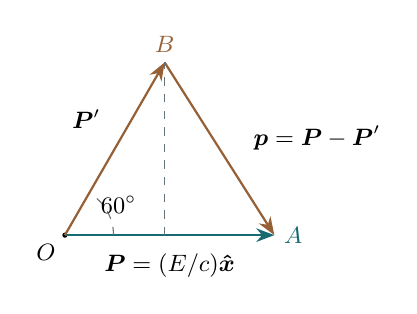
\begin{tikzpicture}[scale=.95,transform shape]
\fill (0,0) circle(.035) node[below left] {$O$};
\draw[motion] (0,0)--(2.8,0) node[right] {$A$};
\draw[motion,color=warm] (0,0)--(1.3331332,2.3090544) node[above] {$B$};
\draw[force] (1.3331332,2.3090544)--(2.8,0);
\draw[guide] (1.3331332,0)--(1.3331332,2.3090544);
\node[below] at (1.4,-.12) {$\boldsymbol P=(E/c)\boldsymbol{\hat x}$};
\node[above left] at (.6,1.3) {$\boldsymbol P^\prime$};
\node[right] at (2.4,1.3) {$\boldsymbol p=\boldsymbol P-\boldsymbol P^\prime$};
\draw[guide] (.65,0) arc(0:60:.65);\node[above] at (.72,.17) {$60^\circ$};
\end{tikzpicture}
\figcaption{解图近1.10A\quad OB与BA首尾相接等于OA，电子动量指向右下方}
\end{minipage}\end{center}
电子总能量为$m_ec^2+K$，其色散关系$(m_ec^2+K)^2=m_e^2c^4+p^2c^2$给$p^2c^2=K(K+2m_ec^2)$。同时，动量三角形的余弦定理给
\[
K=E-E',\quad
p^2c^2=E^2+E'^2-2EE'\cos\theta.
\]
把$K=E-E'$代入前一关系，展开左侧$(E-E')^2+2m_ec^2(E-E')$，再与三角形表达式相等；共同的$E^2+E'^2$相消，剩下
\[
m_ec^2(E-E')=EE'(1-\cos\theta),
\quad
\boxed{\lambda'-\lambda=\lambda_C(1-\cos\theta)}.
\]
最后一步利用$1/E=\lambda/(hc)$、$1/E'=\lambda'/(hc)$。电子吸收正动能对应散射光子能量减小、波长增长。解图近1.10B按固定入射波长画散射角与波长增长，$\theta=60^\circ$处的增长正是$\lambda_C/2$。
\begin{center}\begin{minipage}{.98\linewidth}\centering
\begin{tikzpicture}[scale=.88,transform shape]
\draw[axis] (0,0.0)--(7.3,0.0) node[right] {$\theta/{}^\circ$};
\draw[axis] (0,0)--(0,2.8);
\node[above left] at (0,2.8) {$(\lambda^\prime-\lambda)/\lambda_C$};
\draw[thin] (0.000000,0.0)--(0.000000,-0.06);\node[below,font=\scriptsize] at (0.000000,-0.08) {$ 0 $};
\draw[thin] (2.333333,0.0)--(2.333333,-0.06);\node[below,font=\scriptsize] at (2.333333,-0.08) {$ 60 $};
\draw[thin] (3.500000,0.0)--(3.500000,-0.06);\node[below,font=\scriptsize] at (3.500000,-0.08) {$ 90 $};
\draw[thin] (4.666667,0.0)--(4.666667,-0.06);\node[below,font=\scriptsize] at (4.666667,-0.08) {$ 120 $};
\draw[thin] (7.000000,0.0)--(7.000000,-0.06);\node[below,font=\scriptsize] at (7.000000,-0.08) {$ 180 $};
\draw[thin] (0,0.000000)--(-.06,0.000000);\node[left,font=\scriptsize] at (-.08,0.000000) {$ 0 $};
\draw[thin] (0,0.595238)--(-.06,0.595238);\node[left,font=\scriptsize] at (-.08,0.595238) {$ 0.5 $};
\draw[thin] (0,1.190476)--(-.06,1.190476);\node[left,font=\scriptsize] at (-.08,1.190476) {$ 1 $};
\draw[thin] (0,1.785714)--(-.06,1.785714);\node[left,font=\scriptsize] at (-.08,1.785714) {$ 1.5 $};
\draw[thin] (0,2.380952)--(-.06,2.380952);\node[left,font=\scriptsize] at (-.08,2.380952) {$ 2 $};
\draw[thick,color=accent] plot coordinates {(0.0000000,0.0000000) (0.0291667,0.0001020) (0.0583333,0.0004079) (0.0875000,0.0009178) (0.1166667,0.0016315) (0.1458333,0.0025489) (0.1750000,0.0036698) (0.2041667,0.0049941) (0.2333333,0.0065216) (0.2625000,0.0082518) (0.2916667,0.0101847) (0.3208333,0.0123198) (0.3500000,0.0146567) (0.3791667,0.0171952) (0.4083333,0.0199346) (0.4375000,0.0228747) (0.4666667,0.0260148) (0.4958333,0.0293544) (0.5250000,0.0328930) (0.5541667,0.0366299) (0.5833333,0.0405645) (0.6125000,0.0446961) (0.6416667,0.0490241) (0.6708333,0.0535477) (0.7000000,0.0582661) (0.7291667,0.0631784) (0.7583333,0.0682839) (0.7875000,0.0735817) (0.8166667,0.0790709) (0.8458333,0.0847505) (0.8750000,0.0906196) (0.9041667,0.0966771) (0.9333333,0.1029221) (0.9625000,0.1093534) (0.9916667,0.1159699) (1.0208333,0.1227705) (1.0500000,0.1297541) (1.0791667,0.1369195) (1.1083333,0.1442653) (1.1375000,0.1517905) (1.1666667,0.1594936) (1.1958333,0.1673733) (1.2250000,0.1754284) (1.2541667,0.1836574) (1.2833333,0.1920588) (1.3125000,0.2006314) (1.3416667,0.2093736) (1.3708333,0.2182839) (1.4000000,0.2273607) (1.4291667,0.2366026) (1.4583333,0.2460079) (1.4875000,0.2555751) (1.5166667,0.2653024) (1.5458333,0.2751883) (1.5750000,0.2852310) (1.6041667,0.2954288) (1.6333333,0.3057800) (1.6625000,0.3162827) (1.6916667,0.3269353) (1.7208333,0.3377358) (1.7500000,0.3486824) (1.7791667,0.3597733) (1.8083333,0.3710065) (1.8375000,0.3823801) (1.8666667,0.3938921) (1.8958333,0.4055407) (1.9250000,0.4173238) (1.9541667,0.4292393) (1.9833333,0.4412852) (2.0125000,0.4534596) (2.0416667,0.4657602) (2.0708333,0.4781850) (2.1000000,0.4907318) (2.1291667,0.5033986) (2.1583333,0.5161831) (2.1875000,0.5290831) (2.2166667,0.5420964) (2.2458333,0.5552208) (2.2750000,0.5684541) (2.3041667,0.5817939) (2.3333333,0.5952381) (2.3625000,0.6087842) (2.3916667,0.6224300) (2.4208333,0.6361732) (2.4500000,0.6500113) (2.4791667,0.6639420) (2.5083333,0.6779630) (2.5375000,0.6920717) (2.5666667,0.7062659) (2.5958333,0.7205430) (2.6250000,0.7349007) (2.6541667,0.7493364) (2.6833333,0.7638477) (2.7125000,0.7784321) (2.7416667,0.7930871) (2.7708333,0.8078102) (2.8000000,0.8225988) (2.8291667,0.8374505) (2.8583333,0.8523627) (2.8875000,0.8673328) (2.9166667,0.8823583) (2.9458333,0.8974366) (2.9750000,0.9125650) (3.0041667,0.9277411) (3.0333333,0.9429623) (3.0625000,0.9582258) (3.0916667,0.9735291) (3.1208333,0.9888696) (3.1500000,1.0042447) (3.1791667,1.0196516) (3.2083333,1.0350879) (3.2375000,1.0505507) (3.2666667,1.0660375) (3.2958333,1.0815457) (3.3250000,1.0970725) (3.3541667,1.1126153) (3.3833333,1.1281715) (3.4125000,1.1437383) (3.4416667,1.1593132) (3.4708333,1.1748933) (3.5000000,1.1904762) (3.5291667,1.2060590) (3.5583333,1.2216392) (3.5875000,1.2372141) (3.6166667,1.2527809) (3.6458333,1.2683371) (3.6750000,1.2838799) (3.7041667,1.2994067) (3.7333333,1.3149148) (3.7625000,1.3304017) (3.7916667,1.3458645) (3.8208333,1.3613007) (3.8500000,1.3767077) (3.8791667,1.3920827) (3.9083333,1.4074232) (3.9375000,1.4227266) (3.9666667,1.4379901) (3.9958333,1.4532112) (4.0250000,1.4683873) (4.0541667,1.4835158) (4.0833333,1.4985941) (4.1125000,1.5136196) (4.1416667,1.5285897) (4.1708333,1.5435019) (4.2000000,1.5583536) (4.2291667,1.5731422) (4.2583333,1.5878653) (4.2875000,1.6025203) (4.3166667,1.6171047) (4.3458333,1.6316160) (4.3750000,1.6460517) (4.4041667,1.6604094) (4.4333333,1.6746865) (4.4625000,1.6888806) (4.4916667,1.7029894) (4.5208333,1.7170103) (4.5500000,1.7309411) (4.5791667,1.7447792) (4.6083333,1.7585223) (4.6375000,1.7721681) (4.6666667,1.7857143) (4.6958333,1.7991584) (4.7250000,1.8124983) (4.7541667,1.8257316) (4.7833333,1.8388560) (4.8125000,1.8518693) (4.8416667,1.8647693) (4.8708333,1.8775538) (4.9000000,1.8902205) (4.9291667,1.9027674) (4.9583333,1.9151922) (4.9875000,1.9274928) (5.0166667,1.9396671) (5.0458333,1.9517131) (5.0750000,1.9636286) (5.1041667,1.9754117) (5.1333333,1.9870602) (5.1625000,1.9985723) (5.1916667,2.0099459) (5.2208333,2.0211791) (5.2500000,2.0322700) (5.2791667,2.0432166) (5.3083333,2.0540171) (5.3375000,2.0646697) (5.3666667,2.0751724) (5.3958333,2.0855236) (5.4250000,2.0957214) (5.4541667,2.1057641) (5.4833333,2.1156500) (5.5125000,2.1253773) (5.5416667,2.1349445) (5.5708333,2.1443498) (5.6000000,2.1535917) (5.6291667,2.1626685) (5.6583333,2.1715788) (5.6875000,2.1803210) (5.7166667,2.1888935) (5.7458333,2.1972950) (5.7750000,2.2055240) (5.8041667,2.2135791) (5.8333333,2.2214588) (5.8625000,2.2291619) (5.8916667,2.2366870) (5.9208333,2.2440329) (5.9500000,2.2511982) (5.9791667,2.2581818) (6.0083333,2.2649825) (6.0375000,2.2715990) (6.0666667,2.2780303) (6.0958333,2.2842753) (6.1250000,2.2903328) (6.1541667,2.2962018) (6.1833333,2.3018815) (6.2125000,2.3073706) (6.2416667,2.3126684) (6.2708333,2.3177740) (6.3000000,2.3226863) (6.3291667,2.3274047) (6.3583333,2.3319283) (6.3875000,2.3362562) (6.4166667,2.3403879) (6.4458333,2.3443225) (6.4750000,2.3480594) (6.5041667,2.3515980) (6.5333333,2.3549376) (6.5625000,2.3580777) (6.5916667,2.3610177) (6.6208333,2.3637572) (6.6500000,2.3662956) (6.6791667,2.3686326) (6.7083333,2.3707677) (6.7375000,2.3727005) (6.7666667,2.3744308) (6.7958333,2.3759582) (6.8250000,2.3772825) (6.8541667,2.3784035) (6.8833333,2.3793209) (6.9125000,2.3800346) (6.9416667,2.3805444) (6.9708333,2.3808504) (7.0000000,2.3809524)};
\end{tikzpicture}
\figcaption{解图近1.10B\quad 固定入射波长的康普顿谱移}
\end{minipage}\end{center}
本题给的是末态的散射波长$\lambda'=0.0254\,\mathrm{nm}$，故由位移关系反求入射波长：
\[
\lambda=\lambda'-\frac{\lambda_C}{2}
=0.024186845\,\mathrm{nm},
\]
两光子能量分别约为$E=51.261\,\mathrm{keV}$、$E'=48.813\,\mathrm{keV}$，相减得到
\[
\boxed{K=hc\left(\frac1\lambda-\frac1{\lambda'}\right)
=2.4483\times10^3\,\mathrm{eV}\simeq2.45\,\mathrm{keV}}.
\]
也可把同一个差写成$K=hc\,\Delta\lambda/(\lambda\lambda')$，其中$\Delta\lambda=0.001213155\,\mathrm{nm}$；这个写法直接保留波长差。$\lambda$在能量相减完成前使用上列中间位数，最后按题设数据给$K\simeq2.45\,\mathrm{keV}$。解图近1.10C画固定入射能量下，光子保留的能量与电子获得的能量；两曲线的比例之和始终为1。
\begin{center}\begin{minipage}{.98\linewidth}\centering
\begin{tikzpicture}[scale=.88,transform shape]
\draw[axis] (0,0.0)--(7.3,0.0) node[right] {$\theta/{}^\circ$};
\draw[axis] (0,0)--(0,2.8);
\node[above left] at (0,2.8) {$\text{能量比例}$};
\draw[thin] (0.000000,0.0)--(0.000000,-0.06);\node[below,font=\scriptsize] at (0.000000,-0.08) {$ 0 $};
\draw[thin] (2.333333,0.0)--(2.333333,-0.06);\node[below,font=\scriptsize] at (2.333333,-0.08) {$ 60 $};
\draw[thin] (3.500000,0.0)--(3.500000,-0.06);\node[below,font=\scriptsize] at (3.500000,-0.08) {$ 90 $};
\draw[thin] (4.666667,0.0)--(4.666667,-0.06);\node[below,font=\scriptsize] at (4.666667,-0.08) {$ 120 $};
\draw[thin] (7.000000,0.0)--(7.000000,-0.06);\node[below,font=\scriptsize] at (7.000000,-0.08) {$ 180 $};
\draw[thin] (0,0.000000)--(-.06,0.000000);\node[left,font=\scriptsize] at (-.08,0.000000) {$ 0 $};
\draw[thin] (0,0.595238)--(-.06,0.595238);\node[left,font=\scriptsize] at (-.08,0.595238) {$ 0.25 $};
\draw[thin] (0,1.190476)--(-.06,1.190476);\node[left,font=\scriptsize] at (-.08,1.190476) {$ 0.5 $};
\draw[thin] (0,1.785714)--(-.06,1.785714);\node[left,font=\scriptsize] at (-.08,1.785714) {$ 0.75 $};
\draw[thin] (0,2.380952)--(-.06,2.380952);\node[left,font=\scriptsize] at (-.08,2.380952) {$ 1 $};
\draw[thick,color=accent] plot coordinates {(0.0000000,2.3809524) (0.0291667,2.3809319) (0.0583333,2.3808705) (0.0875000,2.3807683) (0.1166667,2.3806251) (0.1458333,2.3804411) (0.1750000,2.3802163) (0.2041667,2.3799508) (0.2333333,2.3796447) (0.2625000,2.3792980) (0.2916667,2.3789108) (0.3208333,2.3784832) (0.3500000,2.3780154) (0.3791667,2.3775075) (0.4083333,2.3769596) (0.4375000,2.3763719) (0.4666667,2.3757444) (0.4958333,2.3750775) (0.5250000,2.3743713) (0.5541667,2.3736259) (0.5833333,2.3728416) (0.6125000,2.3720186) (0.6416667,2.3711571) (0.6708333,2.3702573) (0.7000000,2.3693195) (0.7291667,2.3683440) (0.7583333,2.3673309) (0.7875000,2.3662806) (0.8166667,2.3651933) (0.8458333,2.3640694) (0.8750000,2.3629091) (0.9041667,2.3617127) (0.9333333,2.3604806) (0.9625000,2.3592131) (0.9916667,2.3579104) (1.0208333,2.3565731) (1.0500000,2.3552013) (1.0791667,2.3537955) (1.1083333,2.3523560) (1.1375000,2.3508832) (1.1666667,2.3493775) (1.1958333,2.3478392) (1.2250000,2.3462688) (1.2541667,2.3446667) (1.2833333,2.3430332) (1.3125000,2.3413688) (1.3416667,2.3396739) (1.3708333,2.3379490) (1.4000000,2.3361944) (1.4291667,2.3344106) (1.4583333,2.3325981) (1.4875000,2.3307572) (1.5166667,2.3288885) (1.5458333,2.3269925) (1.5750000,2.3250695) (1.6041667,2.3231200) (1.6333333,2.3211446) (1.6625000,2.3191437) (1.6916667,2.3171178) (1.7208333,2.3150673) (1.7500000,2.3129928) (1.7791667,2.3108948) (1.8083333,2.3087737) (1.8375000,2.3066300) (1.8666667,2.3044643) (1.8958333,2.3022771) (1.9250000,2.3000688) (1.9541667,2.2978400) (1.9833333,2.2955912) (2.0125000,2.2933229) (2.0416667,2.2910356) (2.0708333,2.2887299) (2.1000000,2.2864062) (2.1291667,2.2840651) (2.1583333,2.2817071) (2.1875000,2.2793327) (2.2166667,2.2769424) (2.2458333,2.2745368) (2.2750000,2.2721164) (2.3041667,2.2696818) (2.3333333,2.2672333) (2.3625000,2.2647716) (2.3916667,2.2622972) (2.4208333,2.2598107) (2.4500000,2.2573124) (2.4791667,2.2548030) (2.5083333,2.2522830) (2.5375000,2.2497529) (2.5666667,2.2472131) (2.5958333,2.2446644) (2.6250000,2.2421070) (2.6541667,2.2395417) (2.6833333,2.2369688) (2.7125000,2.2343889) (2.7416667,2.2318025) (2.7708333,2.2292101) (2.8000000,2.2266122) (2.8291667,2.2240093) (2.8583333,2.2214020) (2.8875000,2.2187906) (2.9166667,2.2161758) (2.9458333,2.2135580) (2.9750000,2.2109376) (3.0041667,2.2083152) (3.0333333,2.2056913) (3.0625000,2.2030664) (3.0916667,2.2004408) (3.1208333,2.1978152) (3.1500000,2.1951899) (3.1791667,2.1925655) (3.2083333,2.1899423) (3.2375000,2.1873209) (3.2666667,2.1847018) (3.2958333,2.1820853) (3.3250000,2.1794719) (3.3541667,2.1768621) (3.3833333,2.1742563) (3.4125000,2.1716550) (3.4416667,2.1690585) (3.4708333,2.1664674) (3.5000000,2.1638820) (3.5291667,2.1613027) (3.5583333,2.1587301) (3.5875000,2.1561644) (3.6166667,2.1536061) (3.6458333,2.1510557) (3.6750000,2.1485135) (3.7041667,2.1459799) (3.7333333,2.1434552) (3.7625000,2.1409400) (3.7916667,2.1384346) (3.8208333,2.1359393) (3.8500000,2.1334545) (3.8791667,2.1309806) (3.9083333,2.1285181) (3.9375000,2.1260671) (3.9666667,2.1236281) (3.9958333,2.1212015) (4.0250000,2.1187876) (4.0541667,2.1163867) (4.0833333,2.1139992) (4.1125000,2.1116253) (4.1416667,2.1092656) (4.1708333,2.1069202) (4.2000000,2.1045895) (4.2291667,2.1022738) (4.2583333,2.0999734) (4.2875000,2.0976887) (4.3166667,2.0954199) (4.3458333,2.0931673) (4.3750000,2.0909313) (4.4041667,2.0887121) (4.4333333,2.0865100) (4.4625000,2.0843253) (4.4916667,2.0821583) (4.5208333,2.0800092) (4.5500000,2.0778783) (4.5791667,2.0757660) (4.6083333,2.0736723) (4.6375000,2.0715977) (4.6666667,2.0695423) (4.6958333,2.0675065) (4.7250000,2.0654903) (4.7541667,2.0634942) (4.7833333,2.0615183) (4.8125000,2.0595628) (4.8416667,2.0576281) (4.8708333,2.0557142) (4.9000000,2.0538215) (4.9291667,2.0519501) (4.9583333,2.0501003) (4.9875000,2.0482723) (5.0166667,2.0464662) (5.0458333,2.0446823) (5.0750000,2.0429208) (5.1041667,2.0411819) (5.1333333,2.0394657) (5.1625000,2.0377724) (5.1916667,2.0361023) (5.2208333,2.0344555) (5.2500000,2.0328321) (5.2791667,2.0312324) (5.3083333,2.0296566) (5.3375000,2.0281047) (5.3666667,2.0265769) (5.3958333,2.0250735) (5.4250000,2.0235945) (5.4541667,2.0221401) (5.4833333,2.0207105) (5.5125000,2.0193057) (5.5416667,2.0179260) (5.5708333,2.0165715) (5.6000000,2.0152423) (5.6291667,2.0139385) (5.6583333,2.0126603) (5.6875000,2.0114077) (5.7166667,2.0101810) (5.7458333,2.0089803) (5.7750000,2.0078055) (5.8041667,2.0066570) (5.8333333,2.0055346) (5.8625000,2.0044387) (5.8916667,2.0033693) (5.9208333,2.0023264) (5.9500000,2.0013102) (5.9791667,2.0003207) (6.0083333,1.9993582) (6.0375000,1.9984225) (6.0666667,1.9975139) (6.0958333,1.9966324) (6.1250000,1.9957782) (6.1541667,1.9949512) (6.1833333,1.9941515) (6.2125000,1.9933793) (6.2416667,1.9926345) (6.2708333,1.9919173) (6.3000000,1.9912278) (6.3291667,1.9905659) (6.3583333,1.9899317) (6.3875000,1.9893254) (6.4166667,1.9887469) (6.4458333,1.9881963) (6.4750000,1.9876736) (6.5041667,1.9871789) (6.5333333,1.9867123) (6.5625000,1.9862738) (6.5916667,1.9858634) (6.6208333,1.9854811) (6.6500000,1.9851270) (6.6791667,1.9848011) (6.7083333,1.9845035) (6.7375000,1.9842341) (6.7666667,1.9839930) (6.7958333,1.9837803) (6.8250000,1.9835959) (6.8541667,1.9834398) (6.8833333,1.9833121) (6.9125000,1.9832127) (6.9416667,1.9831417) (6.9708333,1.9830992) (7.0000000,1.9830850)};
\draw[thick,color=accent] (7.65,2.55)--(8.15,2.55);\node[right,font=\scriptsize] at (8.2,2.55) {$E^\prime/E$};
\draw[thick,dashed,color=warm] plot coordinates {(0.0000000,0.0000000) (0.0291667,0.0000205) (0.0583333,0.0000818) (0.0875000,0.0001841) (0.1166667,0.0003273) (0.1458333,0.0005113) (0.1750000,0.0007361) (0.2041667,0.0010016) (0.2333333,0.0013077) (0.2625000,0.0016544) (0.2916667,0.0020416) (0.3208333,0.0024692) (0.3500000,0.0029370) (0.3791667,0.0034449) (0.4083333,0.0039928) (0.4375000,0.0045805) (0.4666667,0.0052079) (0.4958333,0.0058749) (0.5250000,0.0065811) (0.5541667,0.0073265) (0.5833333,0.0081108) (0.6125000,0.0089338) (0.6416667,0.0097953) (0.6708333,0.0106950) (0.7000000,0.0116328) (0.7291667,0.0126084) (0.7583333,0.0136215) (0.7875000,0.0146718) (0.8166667,0.0157590) (0.8458333,0.0168830) (0.8750000,0.0180433) (0.9041667,0.0192397) (0.9333333,0.0204718) (0.9625000,0.0217393) (0.9916667,0.0230419) (1.0208333,0.0243793) (1.0500000,0.0257511) (1.0791667,0.0271569) (1.1083333,0.0285964) (1.1375000,0.0300692) (1.1666667,0.0315749) (1.1958333,0.0331132) (1.2250000,0.0346836) (1.2541667,0.0362857) (1.2833333,0.0379192) (1.3125000,0.0395836) (1.3416667,0.0412785) (1.3708333,0.0430034) (1.4000000,0.0447580) (1.4291667,0.0465418) (1.4583333,0.0483543) (1.4875000,0.0501952) (1.5166667,0.0520638) (1.5458333,0.0539599) (1.5750000,0.0558829) (1.6041667,0.0578323) (1.6333333,0.0598078) (1.6625000,0.0618087) (1.6916667,0.0638346) (1.7208333,0.0658851) (1.7500000,0.0679596) (1.7791667,0.0700576) (1.8083333,0.0721787) (1.8375000,0.0743224) (1.8666667,0.0764881) (1.8958333,0.0786753) (1.9250000,0.0808836) (1.9541667,0.0831124) (1.9833333,0.0853612) (2.0125000,0.0876295) (2.0416667,0.0899167) (2.0708333,0.0922225) (2.1000000,0.0945462) (2.1291667,0.0968873) (2.1583333,0.0992453) (2.1875000,0.1016197) (2.2166667,0.1040100) (2.2458333,0.1064155) (2.2750000,0.1088359) (2.3041667,0.1112706) (2.3333333,0.1137191) (2.3625000,0.1161807) (2.3916667,0.1186551) (2.4208333,0.1211417) (2.4500000,0.1236400) (2.4791667,0.1261494) (2.5083333,0.1286694) (2.5375000,0.1311995) (2.5666667,0.1337392) (2.5958333,0.1362880) (2.6250000,0.1388454) (2.6541667,0.1414107) (2.6833333,0.1439836) (2.7125000,0.1465635) (2.7416667,0.1491499) (2.7708333,0.1517423) (2.8000000,0.1543402) (2.8291667,0.1569431) (2.8583333,0.1595504) (2.8875000,0.1621618) (2.9166667,0.1647766) (2.9458333,0.1673944) (2.9750000,0.1700148) (3.0041667,0.1726371) (3.0333333,0.1752610) (3.0625000,0.1778860) (3.0916667,0.1805116) (3.1208333,0.1831372) (3.1500000,0.1857625) (3.1791667,0.1883869) (3.2083333,0.1910101) (3.2375000,0.1936314) (3.2666667,0.1962506) (3.2958333,0.1988671) (3.3250000,0.2014805) (3.3541667,0.2040903) (3.3833333,0.2066961) (3.4125000,0.2092974) (3.4416667,0.2118939) (3.4708333,0.2144850) (3.5000000,0.2170704) (3.5291667,0.2196497) (3.5583333,0.2222223) (3.5875000,0.2247880) (3.6166667,0.2273462) (3.6458333,0.2298967) (3.6750000,0.2324389) (3.7041667,0.2349725) (3.7333333,0.2374971) (3.7625000,0.2400124) (3.7916667,0.2425178) (3.8208333,0.2450131) (3.8500000,0.2474979) (3.8791667,0.2499717) (3.9083333,0.2524343) (3.9375000,0.2548853) (3.9666667,0.2573243) (3.9958333,0.2597509) (4.0250000,0.2621648) (4.0541667,0.2645657) (4.0833333,0.2669532) (4.1125000,0.2693270) (4.1416667,0.2716868) (4.1708333,0.2740322) (4.2000000,0.2763629) (4.2291667,0.2786786) (4.2583333,0.2809790) (4.2875000,0.2832637) (4.3166667,0.2855325) (4.3458333,0.2877851) (4.3750000,0.2900211) (4.4041667,0.2922403) (4.4333333,0.2944424) (4.4625000,0.2966271) (4.4916667,0.2987941) (4.5208333,0.3009432) (4.5500000,0.3030740) (4.5791667,0.3051864) (4.6083333,0.3072801) (4.6375000,0.3093547) (4.6666667,0.3114101) (4.6958333,0.3134459) (4.7250000,0.3154621) (4.7541667,0.3174582) (4.7833333,0.3194341) (4.8125000,0.3213895) (4.8416667,0.3233243) (4.8708333,0.3252382) (4.9000000,0.3271309) (4.9291667,0.3290022) (4.9583333,0.3308520) (4.9875000,0.3326801) (5.0166667,0.3344862) (5.0458333,0.3362700) (5.0750000,0.3380316) (5.1041667,0.3397705) (5.1333333,0.3414867) (5.1625000,0.3431799) (5.1916667,0.3448501) (5.2208333,0.3464969) (5.2500000,0.3481202) (5.2791667,0.3497199) (5.3083333,0.3512958) (5.3375000,0.3528477) (5.3666667,0.3543755) (5.3958333,0.3558789) (5.4250000,0.3573579) (5.4541667,0.3588123) (5.4833333,0.3602419) (5.5125000,0.3616467) (5.5416667,0.3630264) (5.5708333,0.3643809) (5.6000000,0.3657101) (5.6291667,0.3670139) (5.6583333,0.3682921) (5.6875000,0.3695446) (5.7166667,0.3707713) (5.7458333,0.3719721) (5.7750000,0.3731469) (5.8041667,0.3742954) (5.8333333,0.3754177) (5.8625000,0.3765137) (5.8916667,0.3775831) (5.9208333,0.3786260) (5.9500000,0.3796422) (5.9791667,0.3806317) (6.0083333,0.3815942) (6.0375000,0.3825299) (6.0666667,0.3834385) (6.0958333,0.3843199) (6.1250000,0.3851742) (6.1541667,0.3860012) (6.1833333,0.3868009) (6.2125000,0.3875731) (6.2416667,0.3883179) (6.2708333,0.3890351) (6.3000000,0.3897246) (6.3291667,0.3903865) (6.3583333,0.3910207) (6.3875000,0.3916270) (6.4166667,0.3922055) (6.4458333,0.3927561) (6.4750000,0.3932788) (6.5041667,0.3937734) (6.5333333,0.3942401) (6.5625000,0.3946786) (6.5916667,0.3950890) (6.6208333,0.3954713) (6.6500000,0.3958254) (6.6791667,0.3961513) (6.7083333,0.3964489) (6.7375000,0.3967183) (6.7666667,0.3969593) (6.7958333,0.3971721) (6.8250000,0.3973565) (6.8541667,0.3975126) (6.8833333,0.3976403) (6.9125000,0.3977397) (6.9416667,0.3978106) (6.9708333,0.3978532) (7.0000000,0.3978674)};
\draw[thick,dashed,color=warm] (7.65,2.0999999999999996)--(8.15,2.0999999999999996);\node[right,font=\scriptsize] at (8.2,2.0999999999999996) {$K/E$};
\end{tikzpicture}
\figcaption{解图近1.10C\quad 同一入射能量分为出射光子和反冲电子动能}
\end{minipage}\end{center}
电子动量大小由解图A的同一个三角形给
\[
p=h\sqrt{\frac1{\lambda^2}+\frac1{\lambda'^2}
-\frac{2\cos\theta}{\lambda\lambda'}}
=\boxed{2.677\times10^{-23}\,\mathrm{kg\,m/s}}.
\]
用$h=6.62607\times10^{-34}\,\mathrm{J\,s}$、波长统一换成米，计算为$2.677\times10^{-23}\,\mathrm{kg\,m/s}$。在$\theta=60^\circ$时，根号内也可合成$(\lambda^2+\lambda'^2-\lambda\lambda')/(\lambda\lambda')^2$，其中混合项的系数为$2\cos60^\circ=1$。该动量还满足前面推得的$pc=\sqrt{K(K+2m_ec^2)}$，这两个式子分别保留矢量方向和电子静能，描述同一反冲状态。

图中$x,y$两轴分别给电子动量分量，
\[
p_x=h\left(\frac1\lambda-\frac{\cos\theta}{\lambda'}\right)>0,\qquad
p_y=-\frac{h\sin\theta}{\lambda'}<0,
\]
于是电子向前且向下运动。若$\varphi$记电子与正$x$轴的锐角，分量之比给
\[
\tan\varphi=\frac{|p_y|}{p_x}
=\frac{\sin\theta}{\lambda'/\lambda-\cos\theta},
\quad \boxed{\varphi=57.57^\circ}.
\]
例如本题$p_x\simeq1.435\times10^{-23}\,\mathrm{kg\,m/s}$、$p_y\simeq-2.259\times10^{-23}\,\mathrm{kg\,m/s}$，负的电子横向动量与向上的散射光子动量相消。解图近1.10D画固定入射波长、$0<\theta\le180^\circ$时的反冲角；当前光子转角60度处，电子反冲角约57.57度。
\begin{center}\begin{minipage}{.98\linewidth}\centering
\begin{tikzpicture}[scale=.88,transform shape]
\draw[axis] (0,0.0)--(7.3,0.0) node[right] {$\theta/{}^\circ$};
\draw[axis] (0,0)--(0,2.8);
\node[above left] at (0,2.8) {$\varphi/{}^\circ$};
\draw[thin] (1.163424,0.0)--(1.163424,-0.06);\node[below,font=\scriptsize] at (1.163424,-0.08) {$ 30 $};
\draw[thin] (2.330739,0.0)--(2.330739,-0.06);\node[below,font=\scriptsize] at (2.330739,-0.08) {$ 60 $};
\draw[thin] (3.498054,0.0)--(3.498054,-0.06);\node[below,font=\scriptsize] at (3.498054,-0.08) {$ 90 $};
\draw[thin] (4.665370,0.0)--(4.665370,-0.06);\node[below,font=\scriptsize] at (4.665370,-0.08) {$ 120 $};
\draw[thin] (7.000000,0.0)--(7.000000,-0.06);\node[below,font=\scriptsize] at (7.000000,-0.08) {$ 180 $};
\draw[thin] (0,0.000000)--(-.06,0.000000);\node[left,font=\scriptsize] at (-.08,0.000000) {$ 0 $};
\draw[thin] (0,0.789474)--(-.06,0.789474);\node[left,font=\scriptsize] at (-.08,0.789474) {$ 30 $};
\draw[thin] (0,1.578947)--(-.06,1.578947);\node[left,font=\scriptsize] at (-.08,1.578947) {$ 60 $};
\draw[thin] (0,2.368421)--(-.06,2.368421);\node[left,font=\scriptsize] at (-.08,2.368421) {$ 90 $};
\draw[thick,color=accent] plot coordinates {(0.0000000,2.3669733) (0.0291667,2.3561210) (0.0583333,2.3452689) (0.0875000,2.3344172) (0.1166667,2.3235662) (0.1458333,2.3127160) (0.1750000,2.3018667) (0.2041667,2.2910187) (0.2333333,2.2801721) (0.2625000,2.2693270) (0.2916667,2.2584837) (0.3208333,2.2476424) (0.3500000,2.2368033) (0.3791667,2.2259665) (0.4083333,2.2151323) (0.4375000,2.2043008) (0.4666667,2.1934723) (0.4958333,2.1826468) (0.5250000,2.1718247) (0.5541667,2.1610060) (0.5833333,2.1501911) (0.6125000,2.1393800) (0.6416667,2.1285730) (0.6708333,2.1177702) (0.7000000,2.1069718) (0.7291667,2.0961780) (0.7583333,2.0853889) (0.7875000,2.0746049) (0.8166667,2.0638259) (0.8458333,2.0530523) (0.8750000,2.0422842) (0.9041667,2.0315217) (0.9333333,2.0207650) (0.9625000,2.0100143) (0.9916667,1.9992698) (1.0208333,1.9885316) (1.0500000,1.9777999) (1.0791667,1.9670749) (1.1083333,1.9563567) (1.1375000,1.9456454) (1.1666667,1.9349413) (1.1958333,1.9242445) (1.2250000,1.9135551) (1.2541667,1.9028733) (1.2833333,1.8921993) (1.3125000,1.8815331) (1.3416667,1.8708750) (1.3708333,1.8602251) (1.4000000,1.8495834) (1.4291667,1.8389503) (1.4583333,1.8283257) (1.4875000,1.8177099) (1.5166667,1.8071030) (1.5458333,1.7965050) (1.5750000,1.7859162) (1.6041667,1.7753367) (1.6333333,1.7647665) (1.6625000,1.7542058) (1.6916667,1.7436547) (1.7208333,1.7331134) (1.7500000,1.7225819) (1.7791667,1.7120604) (1.8083333,1.7015490) (1.8375000,1.6910477) (1.8666667,1.6805567) (1.8958333,1.6700761) (1.9250000,1.6596060) (1.9541667,1.6491465) (1.9833333,1.6386977) (2.0125000,1.6282597) (2.0416667,1.6178325) (2.0708333,1.6074162) (2.1000000,1.5970110) (2.1291667,1.5866170) (2.1583333,1.5762341) (2.1875000,1.5658625) (2.2166667,1.5555023) (2.2458333,1.5451534) (2.2750000,1.5348161) (2.3041667,1.5244904) (2.3333333,1.5141763) (2.3625000,1.5038739) (2.3916667,1.4935832) (2.4208333,1.4833044) (2.4500000,1.4730374) (2.4791667,1.4627823) (2.5083333,1.4525392) (2.5375000,1.4423081) (2.5666667,1.4320891) (2.5958333,1.4218822) (2.6250000,1.4116875) (2.6541667,1.4015049) (2.6833333,1.3913346) (2.7125000,1.3811765) (2.7416667,1.3710307) (2.7708333,1.3608972) (2.8000000,1.3507760) (2.8291667,1.3406672) (2.8583333,1.3305708) (2.8875000,1.3204868) (2.9166667,1.3104152) (2.9458333,1.3003560) (2.9750000,1.2903093) (3.0041667,1.2802750) (3.0333333,1.2702532) (3.0625000,1.2602439) (3.0916667,1.2502470) (3.1208333,1.2402626) (3.1500000,1.2302906) (3.1791667,1.2203311) (3.2083333,1.2103841) (3.2375000,1.2004495) (3.2666667,1.1905273) (3.2958333,1.1806176) (3.3250000,1.1707202) (3.3541667,1.1608353) (3.3833333,1.1509627) (3.4125000,1.1411025) (3.4416667,1.1312545) (3.4708333,1.1214189) (3.5000000,1.1115956) (3.5291667,1.1017845) (3.5583333,1.0919855) (3.5875000,1.0821988) (3.6166667,1.0724242) (3.6458333,1.0626617) (3.6750000,1.0529113) (3.7041667,1.0431729) (3.7333333,1.0334465) (3.7625000,1.0237320) (3.7916667,1.0140294) (3.8208333,1.0043386) (3.8500000,0.9946596) (3.8791667,0.9849924) (3.9083333,0.9753368) (3.9375000,0.9656929) (3.9666667,0.9560605) (3.9958333,0.9464396) (4.0250000,0.9368302) (4.0541667,0.9272322) (4.0833333,0.9176455) (4.1125000,0.9080700) (4.1416667,0.8985058) (4.1708333,0.8889526) (4.2000000,0.8794106) (4.2291667,0.8698795) (4.2583333,0.8603593) (4.2875000,0.8508499) (4.3166667,0.8413514) (4.3458333,0.8318634) (4.3750000,0.8223861) (4.4041667,0.8129194) (4.4333333,0.8034630) (4.4625000,0.7940170) (4.4916667,0.7845813) (4.5208333,0.7751558) (4.5500000,0.7657404) (4.5791667,0.7563350) (4.6083333,0.7469396) (4.6375000,0.7375539) (4.6666667,0.7281781) (4.6958333,0.7188119) (4.7250000,0.7094552) (4.7541667,0.7001080) (4.7833333,0.6907702) (4.8125000,0.6814416) (4.8416667,0.6721223) (4.8708333,0.6628120) (4.9000000,0.6535107) (4.9291667,0.6442182) (4.9583333,0.6349346) (4.9875000,0.6256596) (5.0166667,0.6163931) (5.0458333,0.6071352) (5.0750000,0.5978856) (5.1041667,0.5886442) (5.1333333,0.5794110) (5.1625000,0.5701859) (5.1916667,0.5609686) (5.2208333,0.5517592) (5.2500000,0.5425575) (5.2791667,0.5333633) (5.3083333,0.5241767) (5.3375000,0.5149974) (5.3666667,0.5058254) (5.3958333,0.4966605) (5.4250000,0.4875026) (5.4541667,0.4783517) (5.4833333,0.4692075) (5.5125000,0.4600701) (5.5416667,0.4509391) (5.5708333,0.4418146) (5.6000000,0.4326965) (5.6291667,0.4235845) (5.6583333,0.4144786) (5.6875000,0.4053787) (5.7166667,0.3962846) (5.7458333,0.3871962) (5.7750000,0.3781134) (5.8041667,0.3690361) (5.8333333,0.3599641) (5.8625000,0.3508973) (5.8916667,0.3418357) (5.9208333,0.3327790) (5.9500000,0.3237271) (5.9791667,0.3146800) (6.0083333,0.3056374) (6.0375000,0.2965994) (6.0666667,0.2875656) (6.0958333,0.2785361) (6.1250000,0.2695107) (6.1541667,0.2604892) (6.1833333,0.2514715) (6.2125000,0.2424576) (6.2416667,0.2334472) (6.2708333,0.2244402) (6.3000000,0.2154366) (6.3291667,0.2064361) (6.3583333,0.1974387) (6.3875000,0.1884442) (6.4166667,0.1794525) (6.4458333,0.1704634) (6.4750000,0.1614769) (6.5041667,0.1524927) (6.5333333,0.1435109) (6.5625000,0.1345311) (6.5916667,0.1255533) (6.6208333,0.1165775) (6.6500000,0.1076033) (6.6791667,0.0986307) (6.7083333,0.0896596) (6.7375000,0.0806899) (6.7666667,0.0717213) (6.7958333,0.0627538) (6.8250000,0.0537872) (6.8541667,0.0448215) (6.8833333,0.0358564) (6.9125000,0.0268918) (6.9416667,0.0179277) (6.9708333,0.0089638) (7.0000000,0.0000000)};
\end{tikzpicture}
\figcaption{解图近1.10D\quad 非零反冲电子在散射光另一侧的方向}
\end{minipage}\end{center}
电子在$K/(m_ec^2)\simeq0.00479$的低速区，非相对论动量$\sqrt{2m_eK}$给出接近值；保留相对论式时，精确动量是它的$\sqrt{1+K/(2m_ec^2)}$倍，当前相对差约0.120\%。上面的矢量计算从守恒式到数值均保留了电子静能与正确的反冲方向。


\Needspace{13\baselineskip}

\pdfbookmark[2]{第 11 题 由电子反冲方向求能量}{q11}

\section*{第 11 题\quad 由电子反冲方向求能量}\label{q:11}

光子频率$\nu$与起初静止的自由电子发生康普顿散射。已知反冲电子的运动方向与光子入射方向夹角为$\varphi$，求电子动能；说明物理允许的角度、零反冲退化和最大动能。

\begin{center}\begin{minipage}{.98\linewidth}\centering
\begin{tikzpicture}[scale=.9,transform shape]
\fill (0.00000,0.00000) circle(.035);\node[below left] at (0.00000,0.00000) {$O$};\draw[guide] (0.00000,0.00000)--(3.50000,0.00000);\draw[traj] plot coordinates {(-2.80000,0.00000) (-2.77986,0.01432) (-2.75971,0.02714) (-2.73957,0.03715) (-2.71942,0.04330) (-2.69928,0.04495) (-2.67914,0.04193) (-2.65899,0.03455) (-2.63885,0.02358) (-2.61871,0.01017) (-2.59856,-0.00431) (-2.57842,-0.01833) (-2.55827,-0.03045) (-2.53813,-0.03941) (-2.51799,-0.04427) (-2.49784,-0.04454) (-2.47770,-0.04017) (-2.45755,-0.03163) (-2.43741,-0.01981) (-2.41727,-0.00593) (-2.39712,0.00857) (-2.37698,0.02218) (-2.35683,0.03348) (-2.33669,0.04131) (-2.31655,0.04484) (-2.29640,0.04372) (-2.27626,0.03805) (-2.25612,0.02843) (-2.23597,0.01585) (-2.21583,0.00163) (-2.19568,-0.01276) (-2.17554,-0.02582) (-2.15540,-0.03621) (-2.13525,-0.04283) (-2.11511,-0.04500) (-2.09496,-0.04249) (-2.07482,-0.03557) (-2.05468,-0.02496) (-2.03453,-0.01175) (-2.01439,0.00268) (-1.99424,0.01683) (-1.97410,0.02923) (-1.95396,0.03860) (-1.93381,0.04395) (-1.91367,0.04474) (-1.89353,0.04088) (-1.87338,0.03277) (-1.85324,0.02126) (-1.83309,0.00754) (-1.81295,-0.00696) (-1.79281,-0.02074) (-1.77266,-0.03237) (-1.75252,-0.04063) (-1.73237,-0.04467) (-1.71223,-0.04407) (-1.69209,-0.03889) (-1.67194,-0.02967) (-1.65180,-0.01737) (-1.63165,-0.00326) (-1.61151,0.01118) (-1.59137,0.02447) (-1.57122,0.03521) (-1.55108,0.04230) (-1.53094,0.04499) (-1.51079,0.04300) (-1.49065,0.03655) (-1.47050,0.02630) (-1.45036,0.01332) (-1.43022,-0.00105) (-1.41007,-0.01530) (-1.38993,-0.02797) (-1.36978,-0.03773) (-1.34964,-0.04357) (-1.32950,-0.04489) (-1.30935,-0.04154) (-1.28921,-0.03387) (-1.26906,-0.02269) (-1.24892,-0.00915) (-1.22878,0.00534) (-1.20863,0.01928) (-1.18849,0.03121) (-1.16835,0.03990) (-1.14820,0.04445) (-1.12806,0.04437) (-1.10791,0.03969) (-1.08777,0.03088) (-1.06763,0.01887) (-1.04748,0.00489) (-1.02734,-0.00960) (-1.00719,-0.02308) (-0.98705,-0.03417) (-0.96691,-0.04171) (-0.94676,-0.04492) (-0.92662,-0.04346) (-0.90647,-0.03748) (-0.88633,-0.02761) (-0.86619,-0.01487) (-0.84604,-0.00059) (-0.82590,0.01376) (-0.80576,0.02667) (-0.78561,0.03682) (-0.76547,0.04314) (-0.74532,0.04497) (-0.72518,0.04214) (-0.70504,0.03492) (-0.68489,0.02408) (-0.66475,0.01074) (-0.64460,-0.00372) (-0.62446,-0.01779) (-0.60432,-0.03002) (-0.58417,-0.03912) (-0.56403,-0.04416) (-0.54388,-0.04462) (-0.52374,-0.04043) (-0.50360,-0.03205) (-0.48345,-0.02034) (-0.46331,-0.00651) (-0.44317,0.00799) (-0.42302,0.02167) (-0.40288,0.03309) (-0.38273,0.04107) (-0.36259,0.04479) (-0.34245,0.04385) (-0.32230,0.03836) (-0.30216,0.02888) (-0.28201,0.01640) (-0.26187,0.00222) (-0.24173,-0.01219) (-0.22158,-0.02534) (-0.20144,-0.03585) (-0.18129,-0.04264) (-0.16115,-0.04500) (-0.14101,-0.04268) (-0.12086,-0.03593) (-0.10072,-0.02545) (-0.08058,-0.01232) (-0.06043,0.00209) (-0.04029,0.01628) (-0.02014,0.02878) (0.00000,0.03829)};\draw[motion] (-0.18000,0.00000)--(0.00000,0.00000);\node[above] at (-1.40000,0.00000) {$h/\lambda$};\draw[traj] plot coordinates {(0.00000,0.00000) (-0.00656,0.02383) (-0.01173,0.04714) (-0.01424,0.06949) (-0.01313,0.09053) (-0.00779,0.11002) (0.00194,0.12791) (0.01576,0.14432) (0.03295,0.15950) (0.05245,0.17384) (0.07294,0.18782) (0.09301,0.20195) (0.11129,0.21673) (0.12660,0.23260) (0.13806,0.24986) (0.14519,0.26870) (0.14798,0.28913) (0.14685,0.31097) (0.14263,0.33395) (0.13647,0.35762) (0.12974,0.38151) (0.12384,0.40510) (0.12011,0.42789) (0.11964,0.44950) (0.12321,0.46963) (0.13116,0.48818) (0.14338,0.50517) (0.15931,0.52081) (0.17801,0.53544) (0.19826,0.54950) (0.21868,0.56351) (0.23784,0.57797) (0.25449,0.59335) (0.26760,0.61001) (0.27653,0.62820) (0.28107,0.64798) (0.28146,0.66928) (0.27837,0.69184) (0.27285,0.71528) (0.26618,0.73915) (0.25977,0.76292) (0.25501,0.78609) (0.25310,0.80822) (0.25495,0.82898) (0.26110,0.84818) (0.27162,0.86579) (0.28612,0.88195) (0.30383,0.89694) (0.32361,0.91117) (0.34413,0.92514) (0.36397,0.93936) (0.38179,0.95431) (0.39644,0.97041) (0.40713,0.98796) (0.41345,1.00710) (0.41548,1.02780) (0.41370,1.04988) (0.40903,1.07302) (0.40266,1.09677) (0.39598,1.12064) (0.39038,1.14411) (0.38718,1.16672) (0.38741,1.18807) (0.39177,1.20792) (0.40053,1.22617) (0.41348,1.24289) (0.43000,1.25831) (0.44909,1.27280) (0.46948,1.28682) (0.48976,1.30087) (0.50856,1.31547) (0.52462,1.33106) (0.53700,1.34799) (0.54512,1.36647) (0.54886,1.38654) (0.54855,1.40809) (0.54493,1.43085) (0.53910,1.45441) (0.53237,1.47829) (0.52616,1.50199) (0.52184,1.52500) (0.52056,1.54690) (0.52318,1.56739) (0.53014,1.58629) (0.54143,1.60362) (0.55660,1.61953) (0.57478,1.63435) (0.59480,1.64850) (0.61530,1.66248) (0.63487,1.67679) (0.65218,1.69193) (0.66615,1.70828) (0.67605,1.72611) (0.68157,1.74554) (0.68284,1.76651) (0.68046,1.78882) (0.67538,1.81210) (0.66884,1.83592) (0.66225,1.85975) (0.65701,1.88310) (0.65437,1.90550) (0.65532,1.92659) (0.66048,1.94615) (0.67003,1.96411) (0.68370,1.98057) (0.70078,1.99579) (0.72021,2.01015) (0.74068,2.02414) (0.76080,2.03825) (0.77918,2.05300) (0.79462,2.06882) (0.80625,2.08602) (0.81356,2.10480) (0.81652,2.12515) (0.81553,2.14695) (0.81141,2.16989) (0.80531,2.19354) (0.79857,2.21743) (0.79262,2.24104) (0.78877,2.26387) (0.78816,2.28553) (0.79156,2.30573) (0.79933,2.32434) (0.81138,2.34139) (0.82717,2.35708) (0.84579,2.37174) (0.86601,2.38582) (0.88644,2.39982) (0.90568,2.41425) (0.92245,2.42959) (0.93572,2.44619) (0.94483,2.46432) (0.94954,2.48404) (0.95008,2.50528) (0.94712,2.52779) (0.94167,2.55121) (0.93502,2.57507) (0.92858,2.59885) (0.92372,2.62205) (0.92167,2.64424)};\draw[motion] (0.89609,2.46199)--(0.95766,2.63114);\node[above] at (0.47883,1.31557) {$h/\lambda'$};\draw[force] (0.00000,0.00000)--(1.46674,-1.77163);\node[below right] at (1.46674,-1.77163) {$p_e$};\node[above] at (0.70000,0.35000) {$\theta$};\node[below] at (0.95000,-0.10000) {$\varphi$};\draw[guide] plot coordinates {(0.51017,-0.61622) (0.53335,-0.59627) (0.55575,-0.57545) (0.57734,-0.55379) (0.59808,-0.53132) (0.61795,-0.50807) (0.63692,-0.48408) (0.65495,-0.45938) (0.67203,-0.43402) (0.68813,-0.40801) (0.70322,-0.38142) (0.71729,-0.35426) (0.73030,-0.32659) (0.74225,-0.29844) (0.75311,-0.26985) (0.76288,-0.24087) (0.77153,-0.21154) (0.77905,-0.18189) (0.78543,-0.15199) (0.79066,-0.12186) (0.79474,-0.09155) (0.79766,-0.06111) (0.79942,-0.03058) (0.80000,0.00000)};
\end{tikzpicture}
\figcaption{图近1.11\quad 电子方向角为已知，光子出射方向由守恒确定。}
\end{minipage}\end{center}

\Needspace{6\baselineskip}\subsection*{解答}


图近1.11设入射光子能量$E=h\nu$、动量大小$p_\gamma=E/c$，出射光子动量$p'_\gamma$，电子动量$p_e$、动能$K$。能量守恒给$p'_\gamma c=E-K$。图中两光子的波长分别为$\lambda=c/\nu$与$\lambda'=c/\nu'$，其中$h\nu'=E-K$；动量三角形给
\[
p_\gamma'^2=p_\gamma^2+p_e^2-2p_\gamma p_e\cos\varphi,
\quad p_e^2c^2=K^2+2m_ec^2K.
\]
电子总能量为$E_e=m_ec^2+K$，所以质壳式中的动量项可逐步写成
\[
p_e^2=\frac{E_e^2-(m_ec^2)^2}{c^2}
=\frac{(m_ec^2+K)^2-(m_ec^2)^2}{c^2}
=\frac{K^2+2m_ec^2K}{c^2}.
\]
将$p'_\gamma=(E-K)/c$及$p_\gamma=E/c$代入：
\[
(E-K)^2=E^2+K^2+2m_ec^2K-2Ep_ec\cos\varphi.
\]
左边展开为$E^2-2EK+K^2$，与右边相消$E^2,K^2$后，剩下
\[
-2EK=2m_ec^2K-2Ep_ec\cos\varphi,
\qquad 2Ep_ec\cos\varphi=2K(m_ec^2+E).
\]
消去两边相同项，保留未平方关系
\[
\boxed{K(m_ec^2+E)=Ep_ec\cos\varphi}.
\]
\begin{center}\begin{minipage}{.98\linewidth}\centering
\begin{tikzpicture}[scale=.72,transform shape]
\fill (0.00000,0.00000) circle(.035);\node[below left] at (0.00000,0.00000) {$O$};\draw[guide] (0.00000,0.00000)--(3.50000,0.00000);\draw[traj] plot coordinates {(-2.80000,0.00000) (-2.77986,0.01432) (-2.75971,0.02714) (-2.73957,0.03715) (-2.71942,0.04330) (-2.69928,0.04495) (-2.67914,0.04193) (-2.65899,0.03455) (-2.63885,0.02358) (-2.61871,0.01017) (-2.59856,-0.00431) (-2.57842,-0.01833) (-2.55827,-0.03045) (-2.53813,-0.03941) (-2.51799,-0.04427) (-2.49784,-0.04454) (-2.47770,-0.04017) (-2.45755,-0.03163) (-2.43741,-0.01981) (-2.41727,-0.00593) (-2.39712,0.00857) (-2.37698,0.02218) (-2.35683,0.03348) (-2.33669,0.04131) (-2.31655,0.04484) (-2.29640,0.04372) (-2.27626,0.03805) (-2.25612,0.02843) (-2.23597,0.01585) (-2.21583,0.00163) (-2.19568,-0.01276) (-2.17554,-0.02582) (-2.15540,-0.03621) (-2.13525,-0.04283) (-2.11511,-0.04500) (-2.09496,-0.04249) (-2.07482,-0.03557) (-2.05468,-0.02496) (-2.03453,-0.01175) (-2.01439,0.00268) (-1.99424,0.01683) (-1.97410,0.02923) (-1.95396,0.03860) (-1.93381,0.04395) (-1.91367,0.04474) (-1.89353,0.04088) (-1.87338,0.03277) (-1.85324,0.02126) (-1.83309,0.00754) (-1.81295,-0.00696) (-1.79281,-0.02074) (-1.77266,-0.03237) (-1.75252,-0.04063) (-1.73237,-0.04467) (-1.71223,-0.04407) (-1.69209,-0.03889) (-1.67194,-0.02967) (-1.65180,-0.01737) (-1.63165,-0.00326) (-1.61151,0.01118) (-1.59137,0.02447) (-1.57122,0.03521) (-1.55108,0.04230) (-1.53094,0.04499) (-1.51079,0.04300) (-1.49065,0.03655) (-1.47050,0.02630) (-1.45036,0.01332) (-1.43022,-0.00105) (-1.41007,-0.01530) (-1.38993,-0.02797) (-1.36978,-0.03773) (-1.34964,-0.04357) (-1.32950,-0.04489) (-1.30935,-0.04154) (-1.28921,-0.03387) (-1.26906,-0.02269) (-1.24892,-0.00915) (-1.22878,0.00534) (-1.20863,0.01928) (-1.18849,0.03121) (-1.16835,0.03990) (-1.14820,0.04445) (-1.12806,0.04437) (-1.10791,0.03969) (-1.08777,0.03088) (-1.06763,0.01887) (-1.04748,0.00489) (-1.02734,-0.00960) (-1.00719,-0.02308) (-0.98705,-0.03417) (-0.96691,-0.04171) (-0.94676,-0.04492) (-0.92662,-0.04346) (-0.90647,-0.03748) (-0.88633,-0.02761) (-0.86619,-0.01487) (-0.84604,-0.00059) (-0.82590,0.01376) (-0.80576,0.02667) (-0.78561,0.03682) (-0.76547,0.04314) (-0.74532,0.04497) (-0.72518,0.04214) (-0.70504,0.03492) (-0.68489,0.02408) (-0.66475,0.01074) (-0.64460,-0.00372) (-0.62446,-0.01779) (-0.60432,-0.03002) (-0.58417,-0.03912) (-0.56403,-0.04416) (-0.54388,-0.04462) (-0.52374,-0.04043) (-0.50360,-0.03205) (-0.48345,-0.02034) (-0.46331,-0.00651) (-0.44317,0.00799) (-0.42302,0.02167) (-0.40288,0.03309) (-0.38273,0.04107) (-0.36259,0.04479) (-0.34245,0.04385) (-0.32230,0.03836) (-0.30216,0.02888) (-0.28201,0.01640) (-0.26187,0.00222) (-0.24173,-0.01219) (-0.22158,-0.02534) (-0.20144,-0.03585) (-0.18129,-0.04264) (-0.16115,-0.04500) (-0.14101,-0.04268) (-0.12086,-0.03593) (-0.10072,-0.02545) (-0.08058,-0.01232) (-0.06043,0.00209) (-0.04029,0.01628) (-0.02014,0.02878) (0.00000,0.03829)};\draw[motion] (-0.18000,0.00000)--(0.00000,0.00000);\node[above] at (-1.40000,0.00000) {$h/\lambda$};\draw[traj] plot coordinates {(0.00000,0.00000) (-0.00656,0.02383) (-0.01173,0.04714) (-0.01424,0.06949) (-0.01313,0.09053) (-0.00779,0.11002) (0.00194,0.12791) (0.01576,0.14432) (0.03295,0.15950) (0.05245,0.17384) (0.07294,0.18782) (0.09301,0.20195) (0.11129,0.21673) (0.12660,0.23260) (0.13806,0.24986) (0.14519,0.26870) (0.14798,0.28913) (0.14685,0.31097) (0.14263,0.33395) (0.13647,0.35762) (0.12974,0.38151) (0.12384,0.40510) (0.12011,0.42789) (0.11964,0.44950) (0.12321,0.46963) (0.13116,0.48818) (0.14338,0.50517) (0.15931,0.52081) (0.17801,0.53544) (0.19826,0.54950) (0.21868,0.56351) (0.23784,0.57797) (0.25449,0.59335) (0.26760,0.61001) (0.27653,0.62820) (0.28107,0.64798) (0.28146,0.66928) (0.27837,0.69184) (0.27285,0.71528) (0.26618,0.73915) (0.25977,0.76292) (0.25501,0.78609) (0.25310,0.80822) (0.25495,0.82898) (0.26110,0.84818) (0.27162,0.86579) (0.28612,0.88195) (0.30383,0.89694) (0.32361,0.91117) (0.34413,0.92514) (0.36397,0.93936) (0.38179,0.95431) (0.39644,0.97041) (0.40713,0.98796) (0.41345,1.00710) (0.41548,1.02780) (0.41370,1.04988) (0.40903,1.07302) (0.40266,1.09677) (0.39598,1.12064) (0.39038,1.14411) (0.38718,1.16672) (0.38741,1.18807) (0.39177,1.20792) (0.40053,1.22617) (0.41348,1.24289) (0.43000,1.25831) (0.44909,1.27280) (0.46948,1.28682) (0.48976,1.30087) (0.50856,1.31547) (0.52462,1.33106) (0.53700,1.34799) (0.54512,1.36647) (0.54886,1.38654) (0.54855,1.40809) (0.54493,1.43085) (0.53910,1.45441) (0.53237,1.47829) (0.52616,1.50199) (0.52184,1.52500) (0.52056,1.54690) (0.52318,1.56739) (0.53014,1.58629) (0.54143,1.60362) (0.55660,1.61953) (0.57478,1.63435) (0.59480,1.64850) (0.61530,1.66248) (0.63487,1.67679) (0.65218,1.69193) (0.66615,1.70828) (0.67605,1.72611) (0.68157,1.74554) (0.68284,1.76651) (0.68046,1.78882) (0.67538,1.81210) (0.66884,1.83592) (0.66225,1.85975) (0.65701,1.88310) (0.65437,1.90550) (0.65532,1.92659) (0.66048,1.94615) (0.67003,1.96411) (0.68370,1.98057) (0.70078,1.99579) (0.72021,2.01015) (0.74068,2.02414) (0.76080,2.03825) (0.77918,2.05300) (0.79462,2.06882) (0.80625,2.08602) (0.81356,2.10480) (0.81652,2.12515) (0.81553,2.14695) (0.81141,2.16989) (0.80531,2.19354) (0.79857,2.21743) (0.79262,2.24104) (0.78877,2.26387) (0.78816,2.28553) (0.79156,2.30573) (0.79933,2.32434) (0.81138,2.34139) (0.82717,2.35708) (0.84579,2.37174) (0.86601,2.38582) (0.88644,2.39982) (0.90568,2.41425) (0.92245,2.42959) (0.93572,2.44619) (0.94483,2.46432) (0.94954,2.48404) (0.95008,2.50528) (0.94712,2.52779) (0.94167,2.55121) (0.93502,2.57507) (0.92858,2.59885) (0.92372,2.62205) (0.92167,2.64424)};\draw[motion] (0.89609,2.46199)--(0.95766,2.63114);\node[above] at (0.47883,1.31557) {$h/\lambda'$};\draw[force] (0.00000,0.00000)--(1.46674,-1.77163);\node[below right] at (1.46674,-1.77163) {$p_e$};\node[above] at (0.70000,0.35000) {$\theta$};\node[below] at (0.95000,-0.10000) {$\varphi$};\draw[guide] plot coordinates {(0.51017,-0.61622) (0.53335,-0.59627) (0.55575,-0.57545) (0.57734,-0.55379) (0.59808,-0.53132) (0.61795,-0.50807) (0.63692,-0.48408) (0.65495,-0.45938) (0.67203,-0.43402) (0.68813,-0.40801) (0.70322,-0.38142) (0.71729,-0.35426) (0.73030,-0.32659) (0.74225,-0.29844) (0.75311,-0.26985) (0.76288,-0.24087) (0.77153,-0.21154) (0.77905,-0.18189) (0.78543,-0.15199) (0.79066,-0.12186) (0.79474,-0.09155) (0.79766,-0.06111) (0.79942,-0.03058) (0.80000,0.00000)};\node[below] at (1.00000,-2.40000) {未平方：$K(m_ec^2+E)=Ep_ec\cos\varphi$};\begin{scope}[shift={(7.00000,-0.20000)}]
\draw[axis] (0.00000,0.00000)--(5.25000,0.00000);\draw[axis] (0.00000,0.00000)--(0.00000,2.25000);\node[right] at (5.25000,0.00000) {$\varphi$};\node[above right] at (0.00000,2.25000) {$K/E$，取 $E=m_ec^2$};\draw[traj] plot coordinates {(0.00000,2.00000) (0.01000,1.99997) (0.02000,1.99989) (0.03000,1.99976) (0.04000,1.99958) (0.05000,1.99934) (0.06000,1.99905) (0.07000,1.99871) (0.08000,1.99832) (0.09000,1.99787) (0.10000,1.99737) (0.11000,1.99682) (0.12000,1.99621) (0.13000,1.99556) (0.14000,1.99485) (0.15000,1.99409) (0.16000,1.99327) (0.17000,1.99241) (0.18000,1.99149) (0.19000,1.99052) (0.20000,1.98950) (0.21000,1.98843) (0.22000,1.98730) (0.23000,1.98613) (0.24000,1.98490) (0.25000,1.98362) (0.26000,1.98229) (0.27000,1.98091) (0.28000,1.97947) (0.29000,1.97799) (0.30000,1.97645) (0.31000,1.97487) (0.32000,1.97323) (0.33000,1.97154) (0.34000,1.96981) (0.35000,1.96802) (0.36000,1.96618) (0.37000,1.96429) (0.38000,1.96235) (0.39000,1.96037) (0.40000,1.95833) (0.41000,1.95624) (0.42000,1.95411) (0.43000,1.95192) (0.44000,1.94969) (0.45000,1.94741) (0.46000,1.94508) (0.47000,1.94270) (0.48000,1.94027) (0.49000,1.93779) (0.50000,1.93527) (0.51000,1.93270) (0.52000,1.93008) (0.53000,1.92742) (0.54000,1.92470) (0.55000,1.92194) (0.56000,1.91914) (0.57000,1.91629) (0.58000,1.91339) (0.59000,1.91044) (0.60000,1.90745) (0.61000,1.90442) (0.62000,1.90133) (0.63000,1.89821) (0.64000,1.89504) (0.65000,1.89182) (0.66000,1.88856) (0.67000,1.88526) (0.68000,1.88191) (0.69000,1.87852) (0.70000,1.87508) (0.71000,1.87161) (0.72000,1.86809) (0.73000,1.86452) (0.74000,1.86092) (0.75000,1.85727) (0.76000,1.85358) (0.77000,1.84985) (0.78000,1.84607) (0.79000,1.84226) (0.80000,1.83841) (0.81000,1.83451) (0.82000,1.83058) (0.83000,1.82660) (0.84000,1.82259) (0.85000,1.81853) (0.86000,1.81444) (0.87000,1.81031) (0.88000,1.80614) (0.89000,1.80193) (0.90000,1.79769) (0.91000,1.79340) (0.92000,1.78908) (0.93000,1.78472) (0.94000,1.78033) (0.95000,1.77590) (0.96000,1.77143) (0.97000,1.76693) (0.98000,1.76239) (0.99000,1.75782) (1.00000,1.75321) (1.01000,1.74857) (1.02000,1.74389) (1.03000,1.73918) (1.04000,1.73444) (1.05000,1.72966) (1.06000,1.72485) (1.07000,1.72001) (1.08000,1.71513) (1.09000,1.71023) (1.10000,1.70529) (1.11000,1.70032) (1.12000,1.69532) (1.13000,1.69029) (1.14000,1.68523) (1.15000,1.68014) (1.16000,1.67502) (1.17000,1.66987) (1.18000,1.66469) (1.19000,1.65948) (1.20000,1.65424) (1.21000,1.64898) (1.22000,1.64369) (1.23000,1.63837) (1.24000,1.63302) (1.25000,1.62765) (1.26000,1.62225) (1.27000,1.61683) (1.28000,1.61138) (1.29000,1.60590) (1.30000,1.60041) (1.31000,1.59488) (1.32000,1.58933) (1.33000,1.58376) (1.34000,1.57816) (1.35000,1.57254) (1.36000,1.56690) (1.37000,1.56124) (1.38000,1.55555) (1.39000,1.54984) (1.40000,1.54411) (1.41000,1.53836) (1.42000,1.53259) (1.43000,1.52680) (1.44000,1.52099) (1.45000,1.51516) (1.46000,1.50930) (1.47000,1.50343) (1.48000,1.49755) (1.49000,1.49164) (1.50000,1.48571) (1.51000,1.47977) (1.52000,1.47381) (1.53000,1.46783) (1.54000,1.46184) (1.55000,1.45583) (1.56000,1.44980) (1.57000,1.44376) (1.58000,1.43770) (1.59000,1.43163) (1.60000,1.42554) (1.61000,1.41944) (1.62000,1.41333) (1.63000,1.40720) (1.64000,1.40106) (1.65000,1.39490) (1.66000,1.38873) (1.67000,1.38255) (1.68000,1.37636) (1.69000,1.37016) (1.70000,1.36394) (1.71000,1.35772) (1.72000,1.35148) (1.73000,1.34523) (1.74000,1.33898) (1.75000,1.33271) (1.76000,1.32644) (1.77000,1.32015) (1.78000,1.31386) (1.79000,1.30756) (1.80000,1.30125) (1.81000,1.29493) (1.82000,1.28860) (1.83000,1.28227) (1.84000,1.27593) (1.85000,1.26959) (1.86000,1.26323) (1.87000,1.25688) (1.88000,1.25051) (1.89000,1.24414) (1.90000,1.23777) (1.91000,1.23139) (1.92000,1.22501) (1.93000,1.21863) (1.94000,1.21224) (1.95000,1.20584) (1.96000,1.19945) (1.97000,1.19305) (1.98000,1.18664) (1.99000,1.18024) (2.00000,1.17383) (2.01000,1.16743) (2.02000,1.16102) (2.03000,1.15461) (2.04000,1.14820) (2.05000,1.14178) (2.06000,1.13537) (2.07000,1.12896) (2.08000,1.12255) (2.09000,1.11614) (2.10000,1.10973) (2.11000,1.10332) (2.12000,1.09692) (2.13000,1.09051) (2.14000,1.08411) (2.15000,1.07771) (2.16000,1.07131) (2.17000,1.06491) (2.18000,1.05852) (2.19000,1.05213) (2.20000,1.04575) (2.21000,1.03937) (2.22000,1.03299) (2.23000,1.02662) (2.24000,1.02025) (2.25000,1.01389) (2.26000,1.00753) (2.27000,1.00118) (2.28000,0.99483) (2.29000,0.98849) (2.30000,0.98216) (2.31000,0.97583) (2.32000,0.96951) (2.33000,0.96319) (2.34000,0.95689) (2.35000,0.95059) (2.36000,0.94429) (2.37000,0.93801) (2.38000,0.93174) (2.39000,0.92547) (2.40000,0.91921) (2.41000,0.91296) (2.42000,0.90672) (2.43000,0.90049) (2.44000,0.89426) (2.45000,0.88805) (2.46000,0.88185) (2.47000,0.87566) (2.48000,0.86947) (2.49000,0.86330) (2.50000,0.85714) (2.51000,0.85099) (2.52000,0.84486) (2.53000,0.83873) (2.54000,0.83261) (2.55000,0.82651) (2.56000,0.82042) (2.57000,0.81434) (2.58000,0.80827) (2.59000,0.80222) (2.60000,0.79618) (2.61000,0.79015) (2.62000,0.78414) (2.63000,0.77814) (2.64000,0.77215) (2.65000,0.76618) (2.66000,0.76022) (2.67000,0.75427) (2.68000,0.74834) (2.69000,0.74243) (2.70000,0.73653) (2.71000,0.73064) (2.72000,0.72477) (2.73000,0.71891) (2.74000,0.71307) (2.75000,0.70725) (2.76000,0.70144) (2.77000,0.69565) (2.78000,0.68987) (2.79000,0.68411) (2.80000,0.67837) (2.81000,0.67264) (2.82000,0.66694) (2.83000,0.66124) (2.84000,0.65557) (2.85000,0.64991) (2.86000,0.64427) (2.87000,0.63865) (2.88000,0.63304) (2.89000,0.62745) (2.90000,0.62189) (2.91000,0.61634) (2.92000,0.61080) (2.93000,0.60529) (2.94000,0.59980) (2.95000,0.59432) (2.96000,0.58886) (2.97000,0.58343) (2.98000,0.57801) (2.99000,0.57261) (3.00000,0.56723) (3.01000,0.56187) (3.02000,0.55653) (3.03000,0.55121) (3.04000,0.54591) (3.05000,0.54063) (3.06000,0.53538) (3.07000,0.53014) (3.08000,0.52492) (3.09000,0.51972) (3.10000,0.51455) (3.11000,0.50939) (3.12000,0.50426) (3.13000,0.49915) (3.14000,0.49406) (3.15000,0.48899) (3.16000,0.48394) (3.17000,0.47891) (3.18000,0.47391) (3.19000,0.46893) (3.20000,0.46397) (3.21000,0.45903) (3.22000,0.45411) (3.23000,0.44922) (3.24000,0.44435) (3.25000,0.43950) (3.26000,0.43468) (3.27000,0.42988) (3.28000,0.42510) (3.29000,0.42034) (3.30000,0.41561) (3.31000,0.41090) (3.32000,0.40621) (3.33000,0.40155) (3.34000,0.39691) (3.35000,0.39229) (3.36000,0.38770) (3.37000,0.38313) (3.38000,0.37859) (3.39000,0.37407) (3.40000,0.36957) (3.41000,0.36510) (3.42000,0.36065) (3.43000,0.35623) (3.44000,0.35183) (3.45000,0.34746) (3.46000,0.34311) (3.47000,0.33878) (3.48000,0.33448) (3.49000,0.33021) (3.50000,0.32596) (3.51000,0.32173) (3.52000,0.31753) (3.53000,0.31336) (3.54000,0.30921) (3.55000,0.30508) (3.56000,0.30098) (3.57000,0.29691) (3.58000,0.29286) (3.59000,0.28884) (3.60000,0.28484) (3.61000,0.28087) (3.62000,0.27693) (3.63000,0.27301) (3.64000,0.26911) (3.65000,0.26525) (3.66000,0.26140) (3.67000,0.25759) (3.68000,0.25380) (3.69000,0.25004) (3.70000,0.24630) (3.71000,0.24259) (3.72000,0.23891) (3.73000,0.23525) (3.74000,0.23162) (3.75000,0.22802) (3.76000,0.22444) (3.77000,0.22089) (3.78000,0.21737) (3.79000,0.21387) (3.80000,0.21040) (3.81000,0.20696) (3.82000,0.20354) (3.83000,0.20016) (3.84000,0.19679) (3.85000,0.19346) (3.86000,0.19015) (3.87000,0.18687) (3.88000,0.18362) (3.89000,0.18040) (3.90000,0.17720) (3.91000,0.17403) (3.92000,0.17089) (3.93000,0.16777) (3.94000,0.16468) (3.95000,0.16162) (3.96000,0.15859) (3.97000,0.15559) (3.98000,0.15261) (3.99000,0.14966) (4.00000,0.14674) (4.01000,0.14385) (4.02000,0.14098) (4.03000,0.13815) (4.04000,0.13534) (4.05000,0.13255) (4.06000,0.12980) (4.07000,0.12708) (4.08000,0.12438) (4.09000,0.12171) (4.10000,0.11907) (4.11000,0.11646) (4.12000,0.11388) (4.13000,0.11132) (4.14000,0.10879) (4.15000,0.10629) (4.16000,0.10382) (4.17000,0.10138) (4.18000,0.09897) (4.19000,0.09658) (4.20000,0.09423) (4.21000,0.09190) (4.22000,0.08960) (4.23000,0.08733) (4.24000,0.08509) (4.25000,0.08287) (4.26000,0.08069) (4.27000,0.07853) (4.28000,0.07641) (4.29000,0.07431) (4.30000,0.07224) (4.31000,0.07020) (4.32000,0.06819) (4.33000,0.06620) (4.34000,0.06425) (4.35000,0.06232) (4.36000,0.06043) (4.37000,0.05856) (4.38000,0.05672) (4.39000,0.05491) (4.40000,0.05313) (4.41000,0.05138) (4.42000,0.04966) (4.43000,0.04797) (4.44000,0.04630) (4.45000,0.04467) (4.46000,0.04306) (4.47000,0.04149) (4.48000,0.03994) (4.49000,0.03842) (4.50000,0.03693) (4.51000,0.03547) (4.52000,0.03404) (4.53000,0.03264) (4.54000,0.03127) (4.55000,0.02993) (4.56000,0.02862) (4.57000,0.02733) (4.58000,0.02608) (4.59000,0.02485) (4.60000,0.02366) (4.61000,0.02249) (4.62000,0.02135) (4.63000,0.02024) (4.64000,0.01917) (4.65000,0.01812) (4.66000,0.01710) (4.67000,0.01611) (4.68000,0.01515) (4.69000,0.01422) (4.70000,0.01331) (4.71000,0.01244) (4.72000,0.01160) (4.73000,0.01079) (4.74000,0.01000) (4.75000,0.00925) (4.76000,0.00852) (4.77000,0.00783) (4.78000,0.00716) (4.79000,0.00653) (4.80000,0.00592) (4.81000,0.00534) (4.82000,0.00480) (4.83000,0.00428) (4.84000,0.00379) (4.85000,0.00333) (4.86000,0.00290) (4.87000,0.00250) (4.88000,0.00213) (4.89000,0.00179) (4.90000,0.00148) (4.91000,0.00120) (4.92000,0.00095) (4.93000,0.00073) (4.94000,0.00053) (4.95000,0.00037) (4.96000,0.00024) (4.97000,0.00013) (4.98000,0.00006) (4.99000,0.00001) (5.00000,0.00000)};\draw[thin] (0.00000,-0.06000)--(0.00000,0.06000);\node[below] at (0.00000,-0.13000) {0};\draw[thin] (5.00000,-0.06000)--(5.00000,0.06000);\node[below] at (5.00000,-0.13000) {$90^\circ$};\node[below] at (2.50000,-1.00000) {90°为零反冲极限，方向退化};
\end{scope}
\end{tikzpicture}
\figcaption{解图近1.11A\quad 先保留余弦符号，再用动能闭式判定角域。}
\end{minipage}\end{center}
解图近1.11A中的电子反冲箭头指向入射方向的前半空间：对$K>0$，左侧为正，故$\cos\varphi>0$，即$0\leqslant\varphi<\pi/2$。随后平方并代入电子动量，先保留完整的$K^2$与$K$项：
\[
K^2(m_ec^2+E)^2=E^2(K^2+2m_ec^2K)\cos^2\varphi.
\]
对$K>0$除以$K$，得到
\[
K(m_ec^2+E)^2=E^2(K+2m_ec^2)\cos^2\varphi,
\]
\[
\boxed{K=\frac{2E^2m_ec^2\cos^2\varphi}
{(m_ec^2+E)^2-E^2\cos^2\varphi}}.
\]
用$p_\gamma=E/c$，同一结果的动量形式为
\[
K=\frac{2p_\gamma^2m_e\cos^2\varphi}
{(m_e+p_\gamma/c)^2-(p_\gamma^2/c^2)\cos^2\varphi}.
\]
为说明出射能量，记$M=m_ec^2$与$D=(M+E)^2-E^2\cos^2\varphi$。有$D=M^2+2ME+E^2\sin^2\varphi>0$，并且
\[
E-K=\frac{E[(M+E)^2\sin^2\varphi+M^2\cos^2\varphi]}{D}>0.
\]
因此出射光子保留正能量。未平方关系把含$\cos^2\varphi$的闭式限定在上述前向反冲角域。

解图近1.11B把同一事件的两光子动量和电子动量按统一尺度画为三角形，直接联系角$\varphi$与能量差。
\begin{center}\begin{minipage}{.98\linewidth}\centering
\begin{tikzpicture}[scale=0.9,transform shape]
\draw[motion] (0,0)--(5,0) node[midway,below] {$\boldsymbol p_\gamma$};
\draw[motion] (0,0)--(2.142857143,2.857142857) node[midway,above left] {$\boldsymbol p'_\gamma$};
\draw[force] (2.142857143,2.857142857)--(5,0) node[midway,above right] {$\boldsymbol p_e$};
\draw[guide] (2.142857143,2.857142857)--(2.142857143,0);\fill (0,0) circle(.03);\fill (5,0) circle(.03);\fill (2.142857143,2.857142857) circle(.03);
\node[below] at (2.5,-.8) {$E/(m_ec^2)=1,\quad\varphi=45^\circ,\quad K/E=0.2857143$};
\node[above] at (2.5,3.5571429) {$\boldsymbol p_\gamma=\boldsymbol p'_\gamma+\boldsymbol p_e$};\end{tikzpicture}
\figcaption{解图近1.11B\quad 按同一比例画出的动量三角形：两个光子动量的矢量差为电子动量}
\end{minipage}\end{center}

将$u=\cos^2\varphi$看作变量，写$K=Au/(B-Cu)$，其中$A=2E^2M$、$B=(M+E)^2$、$C=E^2$。其导数为$\mathrm dK/\mathrm du=AB/(B-Cu)^2>0$，故$K$随$u$单调增加。因此$\varphi=0$时最大，
\[
\boxed{K_{\max}=\frac{2E^2}{m_ec^2+2E}},
\]
此时$p_ec=\sqrt{K_{\max}(K_{\max}+2m_ec^2)}=2E(E+m_ec^2)/(m_ec^2+2E)>E$，故动量守恒给$p'_{\gamma x}=E/c-p_e<0$，出射光子沿入射轴反向运动。$\varphi\to\pi/2$时$K\to0$；精确$K=0$时电子动量为零，运动方向未定义；$\varphi\to\pi/2$描述非零反冲事件趋于零动量的过程。若入射光子能量远小于电子静能，公式近似为$K\simeq2E^2\cos^2\varphi/(m_ec^2)$。


\Needspace{13\baselineskip}

\pdfbookmark[2]{第 12 题 最大能量转移反求入射波长}{q12}

\section*{第 12 题\quad 最大能量转移反求入射波长}\label{q:12}

一次光子与静止自由电子的康普顿散射中，可传给电子的最大动能为$K_{\max}=4.5\times10^4\,\mathrm{eV}$。求入射光子真空波长。取$m_ec^2=510999\,\mathrm{eV}$、$hc=1239.84\,\mathrm{eV\,nm}$。

\begin{center}\begin{minipage}{.98\linewidth}\centering
\begin{tikzpicture}[scale=.9,transform shape]
\draw[traj] plot coordinates {(-3.00000,1.00000) (-2.97842,1.01432) (-2.95683,1.02714) (-2.93525,1.03715) (-2.91367,1.04330) (-2.89209,1.04495) (-2.87050,1.04193) (-2.84892,1.03455) (-2.82734,1.02358) (-2.80576,1.01017) (-2.78417,0.99569) (-2.76259,0.98167) (-2.74101,0.96955) (-2.71942,0.96059) (-2.69784,0.95573) (-2.67626,0.95546) (-2.65468,0.95983) (-2.63309,0.96837) (-2.61151,0.98019) (-2.58993,0.99407) (-2.56835,1.00857) (-2.54676,1.02218) (-2.52518,1.03348) (-2.50360,1.04131) (-2.48201,1.04484) (-2.46043,1.04372) (-2.43885,1.03805) (-2.41727,1.02843) (-2.39568,1.01585) (-2.37410,1.00163) (-2.35252,0.98724) (-2.33094,0.97418) (-2.30935,0.96379) (-2.28777,0.95717) (-2.26619,0.95500) (-2.24460,0.95751) (-2.22302,0.96443) (-2.20144,0.97504) (-2.17986,0.98825) (-2.15827,1.00268) (-2.13669,1.01683) (-2.11511,1.02923) (-2.09353,1.03860) (-2.07194,1.04395) (-2.05036,1.04474) (-2.02878,1.04088) (-2.00719,1.03277) (-1.98561,1.02126) (-1.96403,1.00754) (-1.94245,0.99304) (-1.92086,0.97926) (-1.89928,0.96763) (-1.87770,0.95937) (-1.85612,0.95533) (-1.83453,0.95593) (-1.81295,0.96111) (-1.79137,0.97033) (-1.76978,0.98263) (-1.74820,0.99674) (-1.72662,1.01118) (-1.70504,1.02447) (-1.68345,1.03521) (-1.66187,1.04230) (-1.64029,1.04499) (-1.61871,1.04300) (-1.59712,1.03655) (-1.57554,1.02630) (-1.55396,1.01332) (-1.53237,0.99895) (-1.51079,0.98470) (-1.48921,0.97203) (-1.46763,0.96227) (-1.44604,0.95643) (-1.42446,0.95511) (-1.40288,0.95846) (-1.38129,0.96613) (-1.35971,0.97731) (-1.33813,0.99085) (-1.31655,1.00534) (-1.29496,1.01928) (-1.27338,1.03121) (-1.25180,1.03990) (-1.23022,1.04445) (-1.20863,1.04437) (-1.18705,1.03969) (-1.16547,1.03088) (-1.14388,1.01887) (-1.12230,1.00489) (-1.10072,0.99040) (-1.07914,0.97692) (-1.05755,0.96583) (-1.03597,0.95829) (-1.01439,0.95508) (-0.99281,0.95654) (-0.97122,0.96252) (-0.94964,0.97239) (-0.92806,0.98513) (-0.90647,0.99941) (-0.88489,1.01376) (-0.86331,1.02667) (-0.84173,1.03682) (-0.82014,1.04314) (-0.79856,1.04497) (-0.77698,1.04214) (-0.75540,1.03492) (-0.73381,1.02408) (-0.71223,1.01074) (-0.69065,0.99628) (-0.66906,0.98221) (-0.64748,0.96998) (-0.62590,0.96088) (-0.60432,0.95584) (-0.58273,0.95538) (-0.56115,0.95957) (-0.53957,0.96795) (-0.51799,0.97966) (-0.49640,0.99349) (-0.47482,1.00799) (-0.45324,1.02167) (-0.43165,1.03309) (-0.41007,1.04107) (-0.38849,1.04479) (-0.36691,1.04385) (-0.34532,1.03836) (-0.32374,1.02888) (-0.30216,1.01640) (-0.28058,1.00222) (-0.25899,0.98781) (-0.23741,0.97466) (-0.21583,0.96415) (-0.19424,0.95736) (-0.17266,0.95500) (-0.15108,0.95732) (-0.12950,0.96407) (-0.10791,0.97455) (-0.08633,0.98768) (-0.06475,1.00209) (-0.04317,1.01628) (-0.02158,1.02878) (0.00000,1.03829)};\draw[motion] (-0.18000,1.00000)--(0.00000,1.00000);\node[above] at (-1.50000,1.00000) {$E$};\fill (0.00000,1.00000) circle(.035);\node[right] at (0.00000,1.00000) {静止电子};\node[left] at (-3.00000,1.00000) {初态};\draw[traj] plot coordinates {(0.00000,-0.50000) (-0.01942,-0.51432) (-0.03885,-0.52714) (-0.05827,-0.53715) (-0.07770,-0.54330) (-0.09712,-0.54495) (-0.11655,-0.54193) (-0.13597,-0.53455) (-0.15540,-0.52358) (-0.17482,-0.51017) (-0.19424,-0.49569) (-0.21367,-0.48167) (-0.23309,-0.46955) (-0.25252,-0.46059) (-0.27194,-0.45573) (-0.29137,-0.45546) (-0.31079,-0.45983) (-0.33022,-0.46837) (-0.34964,-0.48019) (-0.36906,-0.49407) (-0.38849,-0.50857) (-0.40791,-0.52218) (-0.42734,-0.53348) (-0.44676,-0.54131) (-0.46619,-0.54484) (-0.48561,-0.54372) (-0.50504,-0.53805) (-0.52446,-0.52843) (-0.54388,-0.51585) (-0.56331,-0.50163) (-0.58273,-0.48724) (-0.60216,-0.47418) (-0.62158,-0.46379) (-0.64101,-0.45717) (-0.66043,-0.45500) (-0.67986,-0.45751) (-0.69928,-0.46443) (-0.71871,-0.47504) (-0.73813,-0.48825) (-0.75755,-0.50268) (-0.77698,-0.51683) (-0.79640,-0.52923) (-0.81583,-0.53860) (-0.83525,-0.54395) (-0.85468,-0.54474) (-0.87410,-0.54088) (-0.89353,-0.53277) (-0.91295,-0.52126) (-0.93237,-0.50754) (-0.95180,-0.49304) (-0.97122,-0.47926) (-0.99065,-0.46763) (-1.01007,-0.45937) (-1.02950,-0.45533) (-1.04892,-0.45593) (-1.06835,-0.46111) (-1.08777,-0.47033) (-1.10719,-0.48263) (-1.12662,-0.49674) (-1.14604,-0.51118) (-1.16547,-0.52447) (-1.18489,-0.53521) (-1.20432,-0.54230) (-1.22374,-0.54499) (-1.24317,-0.54300) (-1.26259,-0.53655) (-1.28201,-0.52630) (-1.30144,-0.51332) (-1.32086,-0.49895) (-1.34029,-0.48470) (-1.35971,-0.47203) (-1.37914,-0.46227) (-1.39856,-0.45643) (-1.41799,-0.45511) (-1.43741,-0.45846) (-1.45683,-0.46613) (-1.47626,-0.47731) (-1.49568,-0.49085) (-1.51511,-0.50534) (-1.53453,-0.51928) (-1.55396,-0.53121) (-1.57338,-0.53990) (-1.59281,-0.54445) (-1.61223,-0.54437) (-1.63165,-0.53969) (-1.65108,-0.53088) (-1.67050,-0.51887) (-1.68993,-0.50489) (-1.70935,-0.49040) (-1.72878,-0.47692) (-1.74820,-0.46583) (-1.76763,-0.45829) (-1.78705,-0.45508) (-1.80647,-0.45654) (-1.82590,-0.46252) (-1.84532,-0.47239) (-1.86475,-0.48513) (-1.88417,-0.49941) (-1.90360,-0.51376) (-1.92302,-0.52667) (-1.94245,-0.53682) (-1.96187,-0.54314) (-1.98129,-0.54497) (-2.00072,-0.54214) (-2.02014,-0.53492) (-2.03957,-0.52408) (-2.05899,-0.51074) (-2.07842,-0.49628) (-2.09784,-0.48221) (-2.11727,-0.46998) (-2.13669,-0.46088) (-2.15612,-0.45584) (-2.17554,-0.45538) (-2.19496,-0.45957) (-2.21439,-0.46795) (-2.23381,-0.47966) (-2.25324,-0.49349) (-2.27266,-0.50799) (-2.29209,-0.52167) (-2.31151,-0.53309) (-2.33094,-0.54107) (-2.35036,-0.54479) (-2.36978,-0.54385) (-2.38921,-0.53836) (-2.40863,-0.52888) (-2.42806,-0.51640) (-2.44748,-0.50222) (-2.46691,-0.48781) (-2.48633,-0.47466) (-2.50576,-0.46415) (-2.52518,-0.45736) (-2.54460,-0.45500) (-2.56403,-0.45732) (-2.58345,-0.46407) (-2.60288,-0.47455) (-2.62230,-0.48768) (-2.64173,-0.50209) (-2.66115,-0.51628) (-2.68058,-0.52878) (-2.70000,-0.53829)};\draw[motion] (-2.52000,-0.50000)--(-2.70000,-0.50000);\node[above] at (-1.35000,-0.50000) {$E'$};\draw[force] (0.00000,-0.50000)--(3.00000,-0.50000);\node[right] at (3.00000,-0.50000) {$p_e$};\node[left] at (-3.00000,-0.50000) {末态};
\end{tikzpicture}
\figcaption{图近1.12\quad 最大能量转移的一维反向散射几何。}
\end{minipage}\end{center}

\Needspace{6\baselineskip}\subsection*{解答}


从一般散射角求最大传能时的光路。图近1.12以入射方向为轴，令$\alpha=E/(m_ec^2)>0$、
$u=1-\cos\theta\in[0,2]$，能量动量守恒给
\[
E'=\frac E{1+\alpha u},\qquad
K=E-E'=\frac{E\alpha u}{1+\alpha u},\qquad
\frac{\mathrm dK}{\mathrm du}=\frac{E\alpha}{(1+\alpha u)^2}>0.
\]
所以最大能量转移确在$u=2$即$\theta=\pi$。
解图近1.12A的一维几何由此确定：出射光子反向，电子动量沿入射轴向前。

设入射、出射光子能量为$E,E'$，电子动量为$p$。一维动量守恒和能量守恒为
\[
pc=E+E',\qquad K_{\max}=E-E'.
\]
电子总能量为$m_ec^2+K_{\max}$，质壳式逐步给出
\[
p^2c^2=(m_ec^2+K_{\max})^2-(m_ec^2)^2
=K_{\max}^2+2m_ec^2K_{\max}.
\]
将$pc=E+E'$与$K_{\max}=E-E'$相加消去$E'$，再代入刚求出的电子动量，得
\[
2E=K_{\max}+pc
=K_{\max}+\sqrt{K_{\max}^2+2m_ec^2K_{\max}}.
\]
\begin{center}\begin{minipage}{.98\linewidth}\centering
\begin{tikzpicture}[scale=.9,transform shape]
\draw[traj] plot coordinates {(-3.00000,1.00000) (-2.97842,1.01432) (-2.95683,1.02714) (-2.93525,1.03715) (-2.91367,1.04330) (-2.89209,1.04495) (-2.87050,1.04193) (-2.84892,1.03455) (-2.82734,1.02358) (-2.80576,1.01017) (-2.78417,0.99569) (-2.76259,0.98167) (-2.74101,0.96955) (-2.71942,0.96059) (-2.69784,0.95573) (-2.67626,0.95546) (-2.65468,0.95983) (-2.63309,0.96837) (-2.61151,0.98019) (-2.58993,0.99407) (-2.56835,1.00857) (-2.54676,1.02218) (-2.52518,1.03348) (-2.50360,1.04131) (-2.48201,1.04484) (-2.46043,1.04372) (-2.43885,1.03805) (-2.41727,1.02843) (-2.39568,1.01585) (-2.37410,1.00163) (-2.35252,0.98724) (-2.33094,0.97418) (-2.30935,0.96379) (-2.28777,0.95717) (-2.26619,0.95500) (-2.24460,0.95751) (-2.22302,0.96443) (-2.20144,0.97504) (-2.17986,0.98825) (-2.15827,1.00268) (-2.13669,1.01683) (-2.11511,1.02923) (-2.09353,1.03860) (-2.07194,1.04395) (-2.05036,1.04474) (-2.02878,1.04088) (-2.00719,1.03277) (-1.98561,1.02126) (-1.96403,1.00754) (-1.94245,0.99304) (-1.92086,0.97926) (-1.89928,0.96763) (-1.87770,0.95937) (-1.85612,0.95533) (-1.83453,0.95593) (-1.81295,0.96111) (-1.79137,0.97033) (-1.76978,0.98263) (-1.74820,0.99674) (-1.72662,1.01118) (-1.70504,1.02447) (-1.68345,1.03521) (-1.66187,1.04230) (-1.64029,1.04499) (-1.61871,1.04300) (-1.59712,1.03655) (-1.57554,1.02630) (-1.55396,1.01332) (-1.53237,0.99895) (-1.51079,0.98470) (-1.48921,0.97203) (-1.46763,0.96227) (-1.44604,0.95643) (-1.42446,0.95511) (-1.40288,0.95846) (-1.38129,0.96613) (-1.35971,0.97731) (-1.33813,0.99085) (-1.31655,1.00534) (-1.29496,1.01928) (-1.27338,1.03121) (-1.25180,1.03990) (-1.23022,1.04445) (-1.20863,1.04437) (-1.18705,1.03969) (-1.16547,1.03088) (-1.14388,1.01887) (-1.12230,1.00489) (-1.10072,0.99040) (-1.07914,0.97692) (-1.05755,0.96583) (-1.03597,0.95829) (-1.01439,0.95508) (-0.99281,0.95654) (-0.97122,0.96252) (-0.94964,0.97239) (-0.92806,0.98513) (-0.90647,0.99941) (-0.88489,1.01376) (-0.86331,1.02667) (-0.84173,1.03682) (-0.82014,1.04314) (-0.79856,1.04497) (-0.77698,1.04214) (-0.75540,1.03492) (-0.73381,1.02408) (-0.71223,1.01074) (-0.69065,0.99628) (-0.66906,0.98221) (-0.64748,0.96998) (-0.62590,0.96088) (-0.60432,0.95584) (-0.58273,0.95538) (-0.56115,0.95957) (-0.53957,0.96795) (-0.51799,0.97966) (-0.49640,0.99349) (-0.47482,1.00799) (-0.45324,1.02167) (-0.43165,1.03309) (-0.41007,1.04107) (-0.38849,1.04479) (-0.36691,1.04385) (-0.34532,1.03836) (-0.32374,1.02888) (-0.30216,1.01640) (-0.28058,1.00222) (-0.25899,0.98781) (-0.23741,0.97466) (-0.21583,0.96415) (-0.19424,0.95736) (-0.17266,0.95500) (-0.15108,0.95732) (-0.12950,0.96407) (-0.10791,0.97455) (-0.08633,0.98768) (-0.06475,1.00209) (-0.04317,1.01628) (-0.02158,1.02878) (0.00000,1.03829)};\draw[motion] (-0.18000,1.00000)--(0.00000,1.00000);\node[above] at (-1.50000,1.00000) {$E$};\fill (0.00000,1.00000) circle(.035);\node[right] at (0.00000,1.00000) {静止电子};\node[left] at (-3.00000,1.00000) {初态};\draw[traj] plot coordinates {(0.00000,-0.50000) (-0.01942,-0.51432) (-0.03885,-0.52714) (-0.05827,-0.53715) (-0.07770,-0.54330) (-0.09712,-0.54495) (-0.11655,-0.54193) (-0.13597,-0.53455) (-0.15540,-0.52358) (-0.17482,-0.51017) (-0.19424,-0.49569) (-0.21367,-0.48167) (-0.23309,-0.46955) (-0.25252,-0.46059) (-0.27194,-0.45573) (-0.29137,-0.45546) (-0.31079,-0.45983) (-0.33022,-0.46837) (-0.34964,-0.48019) (-0.36906,-0.49407) (-0.38849,-0.50857) (-0.40791,-0.52218) (-0.42734,-0.53348) (-0.44676,-0.54131) (-0.46619,-0.54484) (-0.48561,-0.54372) (-0.50504,-0.53805) (-0.52446,-0.52843) (-0.54388,-0.51585) (-0.56331,-0.50163) (-0.58273,-0.48724) (-0.60216,-0.47418) (-0.62158,-0.46379) (-0.64101,-0.45717) (-0.66043,-0.45500) (-0.67986,-0.45751) (-0.69928,-0.46443) (-0.71871,-0.47504) (-0.73813,-0.48825) (-0.75755,-0.50268) (-0.77698,-0.51683) (-0.79640,-0.52923) (-0.81583,-0.53860) (-0.83525,-0.54395) (-0.85468,-0.54474) (-0.87410,-0.54088) (-0.89353,-0.53277) (-0.91295,-0.52126) (-0.93237,-0.50754) (-0.95180,-0.49304) (-0.97122,-0.47926) (-0.99065,-0.46763) (-1.01007,-0.45937) (-1.02950,-0.45533) (-1.04892,-0.45593) (-1.06835,-0.46111) (-1.08777,-0.47033) (-1.10719,-0.48263) (-1.12662,-0.49674) (-1.14604,-0.51118) (-1.16547,-0.52447) (-1.18489,-0.53521) (-1.20432,-0.54230) (-1.22374,-0.54499) (-1.24317,-0.54300) (-1.26259,-0.53655) (-1.28201,-0.52630) (-1.30144,-0.51332) (-1.32086,-0.49895) (-1.34029,-0.48470) (-1.35971,-0.47203) (-1.37914,-0.46227) (-1.39856,-0.45643) (-1.41799,-0.45511) (-1.43741,-0.45846) (-1.45683,-0.46613) (-1.47626,-0.47731) (-1.49568,-0.49085) (-1.51511,-0.50534) (-1.53453,-0.51928) (-1.55396,-0.53121) (-1.57338,-0.53990) (-1.59281,-0.54445) (-1.61223,-0.54437) (-1.63165,-0.53969) (-1.65108,-0.53088) (-1.67050,-0.51887) (-1.68993,-0.50489) (-1.70935,-0.49040) (-1.72878,-0.47692) (-1.74820,-0.46583) (-1.76763,-0.45829) (-1.78705,-0.45508) (-1.80647,-0.45654) (-1.82590,-0.46252) (-1.84532,-0.47239) (-1.86475,-0.48513) (-1.88417,-0.49941) (-1.90360,-0.51376) (-1.92302,-0.52667) (-1.94245,-0.53682) (-1.96187,-0.54314) (-1.98129,-0.54497) (-2.00072,-0.54214) (-2.02014,-0.53492) (-2.03957,-0.52408) (-2.05899,-0.51074) (-2.07842,-0.49628) (-2.09784,-0.48221) (-2.11727,-0.46998) (-2.13669,-0.46088) (-2.15612,-0.45584) (-2.17554,-0.45538) (-2.19496,-0.45957) (-2.21439,-0.46795) (-2.23381,-0.47966) (-2.25324,-0.49349) (-2.27266,-0.50799) (-2.29209,-0.52167) (-2.31151,-0.53309) (-2.33094,-0.54107) (-2.35036,-0.54479) (-2.36978,-0.54385) (-2.38921,-0.53836) (-2.40863,-0.52888) (-2.42806,-0.51640) (-2.44748,-0.50222) (-2.46691,-0.48781) (-2.48633,-0.47466) (-2.50576,-0.46415) (-2.52518,-0.45736) (-2.54460,-0.45500) (-2.56403,-0.45732) (-2.58345,-0.46407) (-2.60288,-0.47455) (-2.62230,-0.48768) (-2.64173,-0.50209) (-2.66115,-0.51628) (-2.68058,-0.52878) (-2.70000,-0.53829)};\draw[motion] (-2.52000,-0.50000)--(-2.70000,-0.50000);\node[above] at (-1.35000,-0.50000) {$E'$};\draw[force] (0.00000,-0.50000)--(3.00000,-0.50000);\node[right] at (3.00000,-0.50000) {$p_e$};\node[left] at (-3.00000,-0.50000) {末态};\node[below] at (0.00000,-1.60000) {$E-E'=K_{\max}$，$E+E'=p_ec$};\node[below] at (0.00000,-2.50000) {$p_ec=\sqrt{K_{\max}(K_{\max}+2m_ec^2)}$};
\end{tikzpicture}
\figcaption{解图近1.12A\quad 能量差与动量和联立，得到入射光子正能量。}
\end{minipage}\end{center}
若将已知最大动能暂记为$T$，上式保留了平方前的条件$2E-T=pc>0$。移项后平方，得到
\[
(2E-T)^2=T^2+2m_ec^2T,
\qquad 2E^2-2TE-m_ec^2T=0.
\]
两个二次根为$[T\pm\sqrt{T^2+2m_ec^2T}]/2$。因$T>0$，根式大于$T$，负号根给负的光子能量，正号根同时满足$E>0$和$2E-T>0$，因而确定唯一的入射能量。

解图近1.12B将$2E=K_{\max}+pc$的各项放在同一能量尺度上；这里的$pc$由电子动量换成能量单位，电子动能则为$K_{\max}$。
\begin{center}\begin{minipage}{.98\linewidth}\centering
\begin{tikzpicture}[scale=0.9,transform shape]
\node[anchor=east] at (-.25,2.75) {$E$};\node[anchor=east] at (-.25,1.25) {$K+E^\prime$};\node[anchor=east] at (-.25,-.25) {$K+pc$};\filldraw[fill=accent!15,draw=accent] (0.00000000,2.5) rectangle (3.00000000,3.0);\node at (1.50000000,2.75) {132.062};\filldraw[fill=warm!15,draw=warm] (0.00000000,1.0) rectangle (1.02225085,1.5);\node at (0.51112543,1.25) {45};\filldraw[fill=accent!15,draw=accent] (1.02225085,1.0) rectangle (3.00000000,1.5);\node at (2.01112543,1.25) {87.062};\filldraw[fill=warm!15,draw=warm] (0.00000000,-0.5) rectangle (1.02225085,0.0);\node at (0.51112543,-0.25) {45};\filldraw[fill=accent!15,draw=accent] (1.02225085,-0.5) rectangle (6.00000000,0.0);\node at (3.51112543,-0.25) {219.123};\node[below] at (3,-1.3) {数值单位：keV；同一横向尺度};\end{tikzpicture}
\figcaption{解图近1.12B\quad 电子动能与$pc$之和等于两倍入射能量，横向长度共用同一能量尺度}
\end{minipage}\end{center}

取$m_ec^2=510.999\,\mathrm{keV}$、$hc=1239.84\,\mathrm{eV\,nm}$，由质壳关系取正能量根，
\[
\boxed{E=\frac{K_{\max}+\sqrt{K_{\max}^2+2m_ec^2K_{\max}}}{2}
=1.32062\times10^5\,\mathrm{eV}}.
\]
于是
\[
\boxed{\lambda=\frac{hc}{E}
=9.388\times10^{-3}\,\mathrm{nm}\simeq0.0094\,\mathrm{nm}}.
\]
按题给$K_{\max}$的有效数字，最后用两位数报告约$0.0094\,\mathrm{nm}$，中间数值保留较多位，以便继续计算末光子能量和两波长差。

由$E'=E-K_{\max}=8.7062\times10^4\,\mathrm{eV}>0$，算得$\lambda'=0.01424096\,\mathrm{nm}$。两波长之差为$0.00485261\,\mathrm{nm}=2\lambda_C$，其中$\lambda_C=hc/(m_ec^2)$。入射能量约$132.1\,\mathrm{keV}$分为电子动能$45\,\mathrm{keV}$与反向末光子约$87.1\,\mathrm{keV}$，两者之和保持。


\Needspace{13\baselineskip}

\pdfbookmark[2]{第 13 题 光子与电子散射角的关系}{q13}

\section*{第 13 题\quad 光子与电子散射角的关系}\label{q:13}

在静止自由电子的康普顿散射中，入射光子真空波长为$\lambda$，光子散射角为$\theta$，反冲电子与入射轴的夹角为$\varphi$，电子位于光子散射的另一侧。证明
\[
\cot\frac\theta2=\left(1+\frac{\lambda_C}{\lambda}\right)\tan\varphi,
\qquad \lambda_C=\frac h{m_ec},
\]
并说明两端散射方向的退化情况。

\begin{center}\begin{minipage}{.98\linewidth}\centering
\begin{tikzpicture}[scale=.9,transform shape]
\fill (0.00000,0.00000) circle(.035);\node[below left] at (0.00000,0.00000) {$O$};\draw[guide] (0.00000,0.00000)--(3.50000,0.00000);\draw[traj] plot coordinates {(-2.80000,0.00000) (-2.77986,0.01432) (-2.75971,0.02714) (-2.73957,0.03715) (-2.71942,0.04330) (-2.69928,0.04495) (-2.67914,0.04193) (-2.65899,0.03455) (-2.63885,0.02358) (-2.61871,0.01017) (-2.59856,-0.00431) (-2.57842,-0.01833) (-2.55827,-0.03045) (-2.53813,-0.03941) (-2.51799,-0.04427) (-2.49784,-0.04454) (-2.47770,-0.04017) (-2.45755,-0.03163) (-2.43741,-0.01981) (-2.41727,-0.00593) (-2.39712,0.00857) (-2.37698,0.02218) (-2.35683,0.03348) (-2.33669,0.04131) (-2.31655,0.04484) (-2.29640,0.04372) (-2.27626,0.03805) (-2.25612,0.02843) (-2.23597,0.01585) (-2.21583,0.00163) (-2.19568,-0.01276) (-2.17554,-0.02582) (-2.15540,-0.03621) (-2.13525,-0.04283) (-2.11511,-0.04500) (-2.09496,-0.04249) (-2.07482,-0.03557) (-2.05468,-0.02496) (-2.03453,-0.01175) (-2.01439,0.00268) (-1.99424,0.01683) (-1.97410,0.02923) (-1.95396,0.03860) (-1.93381,0.04395) (-1.91367,0.04474) (-1.89353,0.04088) (-1.87338,0.03277) (-1.85324,0.02126) (-1.83309,0.00754) (-1.81295,-0.00696) (-1.79281,-0.02074) (-1.77266,-0.03237) (-1.75252,-0.04063) (-1.73237,-0.04467) (-1.71223,-0.04407) (-1.69209,-0.03889) (-1.67194,-0.02967) (-1.65180,-0.01737) (-1.63165,-0.00326) (-1.61151,0.01118) (-1.59137,0.02447) (-1.57122,0.03521) (-1.55108,0.04230) (-1.53094,0.04499) (-1.51079,0.04300) (-1.49065,0.03655) (-1.47050,0.02630) (-1.45036,0.01332) (-1.43022,-0.00105) (-1.41007,-0.01530) (-1.38993,-0.02797) (-1.36978,-0.03773) (-1.34964,-0.04357) (-1.32950,-0.04489) (-1.30935,-0.04154) (-1.28921,-0.03387) (-1.26906,-0.02269) (-1.24892,-0.00915) (-1.22878,0.00534) (-1.20863,0.01928) (-1.18849,0.03121) (-1.16835,0.03990) (-1.14820,0.04445) (-1.12806,0.04437) (-1.10791,0.03969) (-1.08777,0.03088) (-1.06763,0.01887) (-1.04748,0.00489) (-1.02734,-0.00960) (-1.00719,-0.02308) (-0.98705,-0.03417) (-0.96691,-0.04171) (-0.94676,-0.04492) (-0.92662,-0.04346) (-0.90647,-0.03748) (-0.88633,-0.02761) (-0.86619,-0.01487) (-0.84604,-0.00059) (-0.82590,0.01376) (-0.80576,0.02667) (-0.78561,0.03682) (-0.76547,0.04314) (-0.74532,0.04497) (-0.72518,0.04214) (-0.70504,0.03492) (-0.68489,0.02408) (-0.66475,0.01074) (-0.64460,-0.00372) (-0.62446,-0.01779) (-0.60432,-0.03002) (-0.58417,-0.03912) (-0.56403,-0.04416) (-0.54388,-0.04462) (-0.52374,-0.04043) (-0.50360,-0.03205) (-0.48345,-0.02034) (-0.46331,-0.00651) (-0.44317,0.00799) (-0.42302,0.02167) (-0.40288,0.03309) (-0.38273,0.04107) (-0.36259,0.04479) (-0.34245,0.04385) (-0.32230,0.03836) (-0.30216,0.02888) (-0.28201,0.01640) (-0.26187,0.00222) (-0.24173,-0.01219) (-0.22158,-0.02534) (-0.20144,-0.03585) (-0.18129,-0.04264) (-0.16115,-0.04500) (-0.14101,-0.04268) (-0.12086,-0.03593) (-0.10072,-0.02545) (-0.08058,-0.01232) (-0.06043,0.00209) (-0.04029,0.01628) (-0.02014,0.02878) (0.00000,0.03829)};\draw[motion] (-0.18000,0.00000)--(0.00000,0.00000);\node[above] at (-1.40000,0.00000) {$h/\lambda$};\draw[traj] plot coordinates {(0.00000,0.00000) (-0.00233,0.02460) (-0.00336,0.04846) (-0.00196,0.07091) (0.00279,0.09143) (0.01143,0.10970) (0.02412,0.12563) (0.04058,0.13939) (0.06015,0.15135) (0.08184,0.16209) (0.10445,0.17230) (0.12667,0.18273) (0.14724,0.19412) (0.16507,0.20708) (0.17935,0.22210) (0.18965,0.23941) (0.19594,0.25904) (0.19862,0.28075) (0.19845,0.30411) (0.19650,0.32849) (0.19402,0.35319) (0.19230,0.37744) (0.19259,0.40053) (0.19588,0.42189) (0.20289,0.44110) (0.21394,0.45799) (0.22892,0.47260) (0.24732,0.48523) (0.26828,0.49639) (0.29067,0.50672) (0.31321,0.51697) (0.33459,0.52789) (0.35366,0.54014) (0.36946,0.55428) (0.38141,0.57064) (0.38932,0.58933) (0.39340,0.61024) (0.39428,0.63299) (0.39291,0.65704) (0.39049,0.68170) (0.38830,0.70622) (0.38764,0.72986) (0.38960,0.75199) (0.39503,0.77212) (0.40442,0.78996) (0.41783,0.80547) (0.43493,0.81886) (0.45497,0.83055) (0.47692,0.84114) (0.49955,0.85133) (0.52156,0.86188) (0.54170,0.87352) (0.55893,0.88683) (0.57250,0.90225) (0.58205,0.92000) (0.58764,0.94003) (0.58973,0.96209) (0.58914,0.98569) (0.58700,1.01019) (0.58456,1.03485) (0.58313,1.05894) (0.58389,1.08176) (0.58783,1.10275) (0.59557,1.12154) (0.60736,1.13799) (0.62302,1.15221) (0.64197,1.16453) (0.66328,1.17548) (0.68580,1.18575) (0.70822,1.19606) (0.72926,1.20717) (0.74778,1.21974) (0.76291,1.23426) (0.77412,1.25105) (0.78130,1.27017) (0.78473,1.29145) (0.78512,1.31448) (0.78346,1.33870) (0.78098,1.36339) (0.77899,1.38780) (0.77872,1.41122) (0.78127,1.43301) (0.78741,1.45272) (0.79754,1.47013) (0.81167,1.48523) (0.82937,1.49828) (0.84985,1.50971) (0.87202,1.52017) (0.89464,1.53037) (0.91639,1.54107) (0.93607,1.55297) (0.95267,1.56665) (0.96552,1.58249) (0.97432,1.60067) (0.97922,1.62110) (0.98074,1.64348) (0.97978,1.66730) (0.97749,1.69188) (0.97514,1.71650) (0.97402,1.74040) (0.97531,1.76292) (0.97991,1.78352) (0.98839,1.80189) (1.00092,1.81792) (1.01724,1.83175) (1.03670,1.84378) (1.05833,1.85455) (1.08092,1.86477) (1.10318,1.87518) (1.12384,1.88651) (1.14180,1.89940) (1.15623,1.91433) (1.16670,1.93154) (1.17315,1.95108) (1.17596,1.97272) (1.17588,1.99602) (1.17398,2.02038) (1.17149,2.04508) (1.16973,2.06936) (1.16991,2.09251) (1.17306,2.11395) (1.17992,2.13325) (1.19080,2.15023) (1.20563,2.16493) (1.22391,2.17763) (1.24479,2.18884) (1.26714,2.19919) (1.28970,2.20943) (1.31115,2.22030) (1.33033,2.23249) (1.34628,2.24654) (1.35840,2.26281) (1.36646,2.28141) (1.37069,2.30223) (1.37168,2.32492) (1.37038,2.34893) (1.36797,2.37358) (1.36576,2.39812) (1.36500,2.42182) (1.36684,2.44402)};\draw[motion] (1.31000,2.26899)--(1.40000,2.42487);\node[above] at (0.70000,1.21244) {$h/\lambda'$};\draw[force] (0.00000,0.00000)--(1.73864,-1.50570);\node[below right] at (1.73864,-1.50570) {$p_e$};\node[above] at (0.70000,0.35000) {$\theta$};\node[below] at (0.95000,-0.10000) {$\varphi$};\draw[guide] plot coordinates {(0.60474,-0.52372) (0.62070,-0.50471) (0.63606,-0.48521) (0.65081,-0.46524) (0.66493,-0.44482) (0.67841,-0.42398) (0.69124,-0.40272) (0.70340,-0.38108) (0.71489,-0.35908) (0.72568,-0.33672) (0.73578,-0.31405) (0.74517,-0.29107) (0.75384,-0.26780) (0.76179,-0.24429) (0.76900,-0.22053) (0.77547,-0.19657) (0.78120,-0.17241) (0.78617,-0.14809) (0.79039,-0.12363) (0.79385,-0.09905) (0.79654,-0.07437) (0.79846,-0.04962) (0.79961,-0.02482) (0.80000,0.00000)};
\end{tikzpicture}
\figcaption{图近1.13\quad 在入射轴两侧分别定义光子角与电子角。}
\end{minipage}\end{center}

\Needspace{6\baselineskip}\subsection*{解答}


图近1.13沿入射光子取$x$，散射光在上方、电子在下方。将动量守恒分解为
\[
\frac h\lambda=\frac h{\lambda'}\cos\theta+p_e\cos\varphi,
\qquad 0=\frac h{\lambda'}\sin\theta-p_e\sin\varphi.
\]
对$0<\theta<\pi$，由两式消去$p_e$：
\[
\tan\varphi=\frac{\sin\theta}{\lambda'/\lambda-\cos\theta}.
\]
\begin{center}\begin{minipage}{.98\linewidth}\centering
\begin{tikzpicture}[scale=.72,transform shape]
\fill (0.00000,0.00000) circle(.035);\node[below left] at (0.00000,0.00000) {$O$};\draw[guide] (0.00000,0.00000)--(3.50000,0.00000);\draw[traj] plot coordinates {(-2.80000,0.00000) (-2.77986,0.01432) (-2.75971,0.02714) (-2.73957,0.03715) (-2.71942,0.04330) (-2.69928,0.04495) (-2.67914,0.04193) (-2.65899,0.03455) (-2.63885,0.02358) (-2.61871,0.01017) (-2.59856,-0.00431) (-2.57842,-0.01833) (-2.55827,-0.03045) (-2.53813,-0.03941) (-2.51799,-0.04427) (-2.49784,-0.04454) (-2.47770,-0.04017) (-2.45755,-0.03163) (-2.43741,-0.01981) (-2.41727,-0.00593) (-2.39712,0.00857) (-2.37698,0.02218) (-2.35683,0.03348) (-2.33669,0.04131) (-2.31655,0.04484) (-2.29640,0.04372) (-2.27626,0.03805) (-2.25612,0.02843) (-2.23597,0.01585) (-2.21583,0.00163) (-2.19568,-0.01276) (-2.17554,-0.02582) (-2.15540,-0.03621) (-2.13525,-0.04283) (-2.11511,-0.04500) (-2.09496,-0.04249) (-2.07482,-0.03557) (-2.05468,-0.02496) (-2.03453,-0.01175) (-2.01439,0.00268) (-1.99424,0.01683) (-1.97410,0.02923) (-1.95396,0.03860) (-1.93381,0.04395) (-1.91367,0.04474) (-1.89353,0.04088) (-1.87338,0.03277) (-1.85324,0.02126) (-1.83309,0.00754) (-1.81295,-0.00696) (-1.79281,-0.02074) (-1.77266,-0.03237) (-1.75252,-0.04063) (-1.73237,-0.04467) (-1.71223,-0.04407) (-1.69209,-0.03889) (-1.67194,-0.02967) (-1.65180,-0.01737) (-1.63165,-0.00326) (-1.61151,0.01118) (-1.59137,0.02447) (-1.57122,0.03521) (-1.55108,0.04230) (-1.53094,0.04499) (-1.51079,0.04300) (-1.49065,0.03655) (-1.47050,0.02630) (-1.45036,0.01332) (-1.43022,-0.00105) (-1.41007,-0.01530) (-1.38993,-0.02797) (-1.36978,-0.03773) (-1.34964,-0.04357) (-1.32950,-0.04489) (-1.30935,-0.04154) (-1.28921,-0.03387) (-1.26906,-0.02269) (-1.24892,-0.00915) (-1.22878,0.00534) (-1.20863,0.01928) (-1.18849,0.03121) (-1.16835,0.03990) (-1.14820,0.04445) (-1.12806,0.04437) (-1.10791,0.03969) (-1.08777,0.03088) (-1.06763,0.01887) (-1.04748,0.00489) (-1.02734,-0.00960) (-1.00719,-0.02308) (-0.98705,-0.03417) (-0.96691,-0.04171) (-0.94676,-0.04492) (-0.92662,-0.04346) (-0.90647,-0.03748) (-0.88633,-0.02761) (-0.86619,-0.01487) (-0.84604,-0.00059) (-0.82590,0.01376) (-0.80576,0.02667) (-0.78561,0.03682) (-0.76547,0.04314) (-0.74532,0.04497) (-0.72518,0.04214) (-0.70504,0.03492) (-0.68489,0.02408) (-0.66475,0.01074) (-0.64460,-0.00372) (-0.62446,-0.01779) (-0.60432,-0.03002) (-0.58417,-0.03912) (-0.56403,-0.04416) (-0.54388,-0.04462) (-0.52374,-0.04043) (-0.50360,-0.03205) (-0.48345,-0.02034) (-0.46331,-0.00651) (-0.44317,0.00799) (-0.42302,0.02167) (-0.40288,0.03309) (-0.38273,0.04107) (-0.36259,0.04479) (-0.34245,0.04385) (-0.32230,0.03836) (-0.30216,0.02888) (-0.28201,0.01640) (-0.26187,0.00222) (-0.24173,-0.01219) (-0.22158,-0.02534) (-0.20144,-0.03585) (-0.18129,-0.04264) (-0.16115,-0.04500) (-0.14101,-0.04268) (-0.12086,-0.03593) (-0.10072,-0.02545) (-0.08058,-0.01232) (-0.06043,0.00209) (-0.04029,0.01628) (-0.02014,0.02878) (0.00000,0.03829)};\draw[motion] (-0.18000,0.00000)--(0.00000,0.00000);\node[above] at (-1.40000,0.00000) {$h/\lambda$};\draw[traj] plot coordinates {(0.00000,0.00000) (-0.00233,0.02460) (-0.00336,0.04846) (-0.00196,0.07091) (0.00279,0.09143) (0.01143,0.10970) (0.02412,0.12563) (0.04058,0.13939) (0.06015,0.15135) (0.08184,0.16209) (0.10445,0.17230) (0.12667,0.18273) (0.14724,0.19412) (0.16507,0.20708) (0.17935,0.22210) (0.18965,0.23941) (0.19594,0.25904) (0.19862,0.28075) (0.19845,0.30411) (0.19650,0.32849) (0.19402,0.35319) (0.19230,0.37744) (0.19259,0.40053) (0.19588,0.42189) (0.20289,0.44110) (0.21394,0.45799) (0.22892,0.47260) (0.24732,0.48523) (0.26828,0.49639) (0.29067,0.50672) (0.31321,0.51697) (0.33459,0.52789) (0.35366,0.54014) (0.36946,0.55428) (0.38141,0.57064) (0.38932,0.58933) (0.39340,0.61024) (0.39428,0.63299) (0.39291,0.65704) (0.39049,0.68170) (0.38830,0.70622) (0.38764,0.72986) (0.38960,0.75199) (0.39503,0.77212) (0.40442,0.78996) (0.41783,0.80547) (0.43493,0.81886) (0.45497,0.83055) (0.47692,0.84114) (0.49955,0.85133) (0.52156,0.86188) (0.54170,0.87352) (0.55893,0.88683) (0.57250,0.90225) (0.58205,0.92000) (0.58764,0.94003) (0.58973,0.96209) (0.58914,0.98569) (0.58700,1.01019) (0.58456,1.03485) (0.58313,1.05894) (0.58389,1.08176) (0.58783,1.10275) (0.59557,1.12154) (0.60736,1.13799) (0.62302,1.15221) (0.64197,1.16453) (0.66328,1.17548) (0.68580,1.18575) (0.70822,1.19606) (0.72926,1.20717) (0.74778,1.21974) (0.76291,1.23426) (0.77412,1.25105) (0.78130,1.27017) (0.78473,1.29145) (0.78512,1.31448) (0.78346,1.33870) (0.78098,1.36339) (0.77899,1.38780) (0.77872,1.41122) (0.78127,1.43301) (0.78741,1.45272) (0.79754,1.47013) (0.81167,1.48523) (0.82937,1.49828) (0.84985,1.50971) (0.87202,1.52017) (0.89464,1.53037) (0.91639,1.54107) (0.93607,1.55297) (0.95267,1.56665) (0.96552,1.58249) (0.97432,1.60067) (0.97922,1.62110) (0.98074,1.64348) (0.97978,1.66730) (0.97749,1.69188) (0.97514,1.71650) (0.97402,1.74040) (0.97531,1.76292) (0.97991,1.78352) (0.98839,1.80189) (1.00092,1.81792) (1.01724,1.83175) (1.03670,1.84378) (1.05833,1.85455) (1.08092,1.86477) (1.10318,1.87518) (1.12384,1.88651) (1.14180,1.89940) (1.15623,1.91433) (1.16670,1.93154) (1.17315,1.95108) (1.17596,1.97272) (1.17588,1.99602) (1.17398,2.02038) (1.17149,2.04508) (1.16973,2.06936) (1.16991,2.09251) (1.17306,2.11395) (1.17992,2.13325) (1.19080,2.15023) (1.20563,2.16493) (1.22391,2.17763) (1.24479,2.18884) (1.26714,2.19919) (1.28970,2.20943) (1.31115,2.22030) (1.33033,2.23249) (1.34628,2.24654) (1.35840,2.26281) (1.36646,2.28141) (1.37069,2.30223) (1.37168,2.32492) (1.37038,2.34893) (1.36797,2.37358) (1.36576,2.39812) (1.36500,2.42182) (1.36684,2.44402)};\draw[motion] (1.31000,2.26899)--(1.40000,2.42487);\node[above] at (0.70000,1.21244) {$h/\lambda'$};\draw[force] (0.00000,0.00000)--(1.73864,-1.50570);\node[below right] at (1.73864,-1.50570) {$p_e$};\node[above] at (0.70000,0.35000) {$\theta$};\node[below] at (0.95000,-0.10000) {$\varphi$};\draw[guide] plot coordinates {(0.60474,-0.52372) (0.62070,-0.50471) (0.63606,-0.48521) (0.65081,-0.46524) (0.66493,-0.44482) (0.67841,-0.42398) (0.69124,-0.40272) (0.70340,-0.38108) (0.71489,-0.35908) (0.72568,-0.33672) (0.73578,-0.31405) (0.74517,-0.29107) (0.75384,-0.26780) (0.76179,-0.24429) (0.76900,-0.22053) (0.77547,-0.19657) (0.78120,-0.17241) (0.78617,-0.14809) (0.79039,-0.12363) (0.79385,-0.09905) (0.79654,-0.07437) (0.79846,-0.04962) (0.79961,-0.02482) (0.80000,0.00000)};\node[below] at (0.00000,-2.80000) {$p_e\sin\varphi=(h/\lambda')\sin\theta$};\begin{scope}[shift={(7.00000,0.00000)}]
\draw[axis] (0.00000,0.00000)--(5.25000,0.00000);\draw[axis] (0.00000,0.00000)--(0.00000,2.25000);\node[right] at (5.25000,0.00000) {$\theta$};\node[above right] at (0.00000,2.25000) {$\varphi$（度），$\lambda=\lambda_C$};\draw[traj] plot coordinates {(0.00000,1.99556) (0.01000,1.98756) (0.02000,1.97957) (0.03000,1.97159) (0.04000,1.96360) (0.05000,1.95561) (0.06000,1.94763) (0.07000,1.93965) (0.08000,1.93168) (0.09000,1.92370) (0.10000,1.91574) (0.11000,1.90777) (0.12000,1.89982) (0.13000,1.89187) (0.14000,1.88392) (0.15000,1.87598) (0.16000,1.86805) (0.17000,1.86013) (0.18000,1.85221) (0.19000,1.84431) (0.20000,1.83641) (0.21000,1.82852) (0.22000,1.82065) (0.23000,1.81278) (0.24000,1.80492) (0.25000,1.79707) (0.26000,1.78924) (0.27000,1.78142) (0.28000,1.77361) (0.29000,1.76581) (0.30000,1.75803) (0.31000,1.75026) (0.32000,1.74250) (0.33000,1.73476) (0.34000,1.72703) (0.35000,1.71932) (0.36000,1.71162) (0.37000,1.70394) (0.38000,1.69628) (0.39000,1.68863) (0.40000,1.68100) (0.41000,1.67338) (0.42000,1.66579) (0.43000,1.65821) (0.44000,1.65065) (0.45000,1.64311) (0.46000,1.63558) (0.47000,1.62808) (0.48000,1.62059) (0.49000,1.61313) (0.50000,1.60569) (0.51000,1.59826) (0.52000,1.59086) (0.53000,1.58347) (0.54000,1.57611) (0.55000,1.56877) (0.56000,1.56145) (0.57000,1.55416) (0.58000,1.54688) (0.59000,1.53963) (0.60000,1.53240) (0.61000,1.52519) (0.62000,1.51801) (0.63000,1.51085) (0.64000,1.50371) (0.65000,1.49660) (0.66000,1.48951) (0.67000,1.48244) (0.68000,1.47540) (0.69000,1.46838) (0.70000,1.46139) (0.71000,1.45442) (0.72000,1.44747) (0.73000,1.44056) (0.74000,1.43366) (0.75000,1.42679) (0.76000,1.41995) (0.77000,1.41313) (0.78000,1.40634) (0.79000,1.39957) (0.80000,1.39283) (0.81000,1.38611) (0.82000,1.37942) (0.83000,1.37276) (0.84000,1.36612) (0.85000,1.35951) (0.86000,1.35293) (0.87000,1.34637) (0.88000,1.33984) (0.89000,1.33333) (0.90000,1.32685) (0.91000,1.32040) (0.92000,1.31397) (0.93000,1.30757) (0.94000,1.30120) (0.95000,1.29485) (0.96000,1.28853) (0.97000,1.28224) (0.98000,1.27597) (0.99000,1.26973) (1.00000,1.26352) (1.01000,1.25733) (1.02000,1.25117) (1.03000,1.24504) (1.04000,1.23893) (1.05000,1.23285) (1.06000,1.22680) (1.07000,1.22077) (1.08000,1.21478) (1.09000,1.20880) (1.10000,1.20286) (1.11000,1.19694) (1.12000,1.19104) (1.13000,1.18518) (1.14000,1.17933) (1.15000,1.17352) (1.16000,1.16773) (1.17000,1.16197) (1.18000,1.15623) (1.19000,1.15053) (1.20000,1.14484) (1.21000,1.13918) (1.22000,1.13355) (1.23000,1.12795) (1.24000,1.12237) (1.25000,1.11681) (1.26000,1.11129) (1.27000,1.10578) (1.28000,1.10031) (1.29000,1.09485) (1.30000,1.08943) (1.31000,1.08403) (1.32000,1.07865) (1.33000,1.07330) (1.34000,1.06797) (1.35000,1.06267) (1.36000,1.05739) (1.37000,1.05214) (1.38000,1.04691) (1.39000,1.04171) (1.40000,1.03653) (1.41000,1.03138) (1.42000,1.02625) (1.43000,1.02114) (1.44000,1.01606) (1.45000,1.01100) (1.46000,1.00597) (1.47000,1.00096) (1.48000,0.99597) (1.49000,0.99101) (1.50000,0.98607) (1.51000,0.98115) (1.52000,0.97625) (1.53000,0.97138) (1.54000,0.96653) (1.55000,0.96171) (1.56000,0.95691) (1.57000,0.95213) (1.58000,0.94737) (1.59000,0.94263) (1.60000,0.93792) (1.61000,0.93323) (1.62000,0.92856) (1.63000,0.92391) (1.64000,0.91928) (1.65000,0.91468) (1.66000,0.91009) (1.67000,0.90553) (1.68000,0.90099) (1.69000,0.89647) (1.70000,0.89197) (1.71000,0.88749) (1.72000,0.88304) (1.73000,0.87860) (1.74000,0.87418) (1.75000,0.86979) (1.76000,0.86541) (1.77000,0.86106) (1.78000,0.85672) (1.79000,0.85241) (1.80000,0.84811) (1.81000,0.84383) (1.82000,0.83958) (1.83000,0.83534) (1.84000,0.83112) (1.85000,0.82692) (1.86000,0.82274) (1.87000,0.81858) (1.88000,0.81444) (1.89000,0.81031) (1.90000,0.80621) (1.91000,0.80212) (1.92000,0.79805) (1.93000,0.79400) (1.94000,0.78997) (1.95000,0.78595) (1.96000,0.78196) (1.97000,0.77798) (1.98000,0.77402) (1.99000,0.77007) (2.00000,0.76614) (2.01000,0.76224) (2.02000,0.75834) (2.03000,0.75447) (2.04000,0.75061) (2.05000,0.74677) (2.06000,0.74294) (2.07000,0.73913) (2.08000,0.73534) (2.09000,0.73156) (2.10000,0.72780) (2.11000,0.72406) (2.12000,0.72033) (2.13000,0.71662) (2.14000,0.71292) (2.15000,0.70924) (2.16000,0.70558) (2.17000,0.70193) (2.18000,0.69829) (2.19000,0.69467) (2.20000,0.69107) (2.21000,0.68748) (2.22000,0.68391) (2.23000,0.68035) (2.24000,0.67680) (2.25000,0.67327) (2.26000,0.66976) (2.27000,0.66625) (2.28000,0.66277) (2.29000,0.65929) (2.30000,0.65583) (2.31000,0.65239) (2.32000,0.64896) (2.33000,0.64554) (2.34000,0.64214) (2.35000,0.63875) (2.36000,0.63537) (2.37000,0.63201) (2.38000,0.62865) (2.39000,0.62532) (2.40000,0.62199) (2.41000,0.61868) (2.42000,0.61538) (2.43000,0.61210) (2.44000,0.60882) (2.45000,0.60556) (2.46000,0.60232) (2.47000,0.59908) (2.48000,0.59586) (2.49000,0.59265) (2.50000,0.58945) (2.51000,0.58626) (2.52000,0.58308) (2.53000,0.57992) (2.54000,0.57677) (2.55000,0.57363) (2.56000,0.57050) (2.57000,0.56738) (2.58000,0.56428) (2.59000,0.56118) (2.60000,0.55810) (2.61000,0.55503) (2.62000,0.55197) (2.63000,0.54892) (2.64000,0.54588) (2.65000,0.54285) (2.66000,0.53983) (2.67000,0.53683) (2.68000,0.53383) (2.69000,0.53084) (2.70000,0.52787) (2.71000,0.52490) (2.72000,0.52195) (2.73000,0.51900) (2.74000,0.51607) (2.75000,0.51315) (2.76000,0.51023) (2.77000,0.50733) (2.78000,0.50443) (2.79000,0.50155) (2.80000,0.49867) (2.81000,0.49580) (2.82000,0.49295) (2.83000,0.49010) (2.84000,0.48726) (2.85000,0.48443) (2.86000,0.48161) (2.87000,0.47880) (2.88000,0.47600) (2.89000,0.47321) (2.90000,0.47042) (2.91000,0.46765) (2.92000,0.46488) (2.93000,0.46212) (2.94000,0.45938) (2.95000,0.45664) (2.96000,0.45390) (2.97000,0.45118) (2.98000,0.44846) (2.99000,0.44576) (3.00000,0.44306) (3.01000,0.44037) (3.02000,0.43769) (3.03000,0.43501) (3.04000,0.43234) (3.05000,0.42969) (3.06000,0.42703) (3.07000,0.42439) (3.08000,0.42176) (3.09000,0.41913) (3.10000,0.41651) (3.11000,0.41389) (3.12000,0.41129) (3.13000,0.40869) (3.14000,0.40610) (3.15000,0.40352) (3.16000,0.40094) (3.17000,0.39837) (3.18000,0.39581) (3.19000,0.39325) (3.20000,0.39071) (3.21000,0.38817) (3.22000,0.38563) (3.23000,0.38310) (3.24000,0.38058) (3.25000,0.37807) (3.26000,0.37556) (3.27000,0.37306) (3.28000,0.37057) (3.29000,0.36808) (3.30000,0.36560) (3.31000,0.36312) (3.32000,0.36065) (3.33000,0.35819) (3.34000,0.35573) (3.35000,0.35328) (3.36000,0.35084) (3.37000,0.34840) (3.38000,0.34597) (3.39000,0.34354) (3.40000,0.34112) (3.41000,0.33870) (3.42000,0.33629) (3.43000,0.33389) (3.44000,0.33149) (3.45000,0.32910) (3.46000,0.32671) (3.47000,0.32433) (3.48000,0.32196) (3.49000,0.31959) (3.50000,0.31722) (3.51000,0.31486) (3.52000,0.31251) (3.53000,0.31016) (3.54000,0.30782) (3.55000,0.30548) (3.56000,0.30314) (3.57000,0.30082) (3.58000,0.29849) (3.59000,0.29617) (3.60000,0.29386) (3.61000,0.29155) (3.62000,0.28925) (3.63000,0.28695) (3.64000,0.28465) (3.65000,0.28236) (3.66000,0.28008) (3.67000,0.27780) (3.68000,0.27552) (3.69000,0.27325) (3.70000,0.27098) (3.71000,0.26872) (3.72000,0.26646) (3.73000,0.26420) (3.74000,0.26195) (3.75000,0.25971) (3.76000,0.25747) (3.77000,0.25523) (3.78000,0.25300) (3.79000,0.25077) (3.80000,0.24854) (3.81000,0.24632) (3.82000,0.24410) (3.83000,0.24189) (3.84000,0.23968) (3.85000,0.23747) (3.86000,0.23527) (3.87000,0.23307) (3.88000,0.23088) (3.89000,0.22869) (3.90000,0.22650) (3.91000,0.22432) (3.92000,0.22214) (3.93000,0.21996) (3.94000,0.21779) (3.95000,0.21562) (3.96000,0.21345) (3.97000,0.21129) (3.98000,0.20913) (3.99000,0.20697) (4.00000,0.20482) (4.01000,0.20267) (4.02000,0.20052) (4.03000,0.19838) (4.04000,0.19624) (4.05000,0.19410) (4.06000,0.19197) (4.07000,0.18984) (4.08000,0.18771) (4.09000,0.18558) (4.10000,0.18346) (4.11000,0.18134) (4.12000,0.17922) (4.13000,0.17711) (4.14000,0.17499) (4.15000,0.17289) (4.16000,0.17078) (4.17000,0.16868) (4.18000,0.16658) (4.19000,0.16448) (4.20000,0.16238) (4.21000,0.16029) (4.22000,0.15820) (4.23000,0.15611) (4.24000,0.15402) (4.25000,0.15194) (4.26000,0.14986) (4.27000,0.14778) (4.28000,0.14570) (4.29000,0.14362) (4.30000,0.14155) (4.31000,0.13948) (4.32000,0.13741) (4.33000,0.13535) (4.34000,0.13328) (4.35000,0.13122) (4.36000,0.12916) (4.37000,0.12710) (4.38000,0.12505) (4.39000,0.12299) (4.40000,0.12094) (4.41000,0.11889) (4.42000,0.11684) (4.43000,0.11479) (4.44000,0.11275) (4.45000,0.11070) (4.46000,0.10866) (4.47000,0.10662) (4.48000,0.10458) (4.49000,0.10254) (4.50000,0.10051) (4.51000,0.09847) (4.52000,0.09644) (4.53000,0.09441) (4.54000,0.09238) (4.55000,0.09035) (4.56000,0.08832) (4.57000,0.08630) (4.58000,0.08427) (4.59000,0.08225) (4.60000,0.08023) (4.61000,0.07821) (4.62000,0.07619) (4.63000,0.07417) (4.64000,0.07215) (4.65000,0.07013) (4.66000,0.06812) (4.67000,0.06610) (4.68000,0.06409) (4.69000,0.06208) (4.70000,0.06007) (4.71000,0.05806) (4.72000,0.05605) (4.73000,0.05404) (4.74000,0.05203) (4.75000,0.05002) (4.76000,0.04801) (4.77000,0.04601) (4.78000,0.04400) (4.79000,0.04200) (4.80000,0.03999) (4.81000,0.03799) (4.82000,0.03599) (4.83000,0.03399) (4.84000,0.03198) (4.85000,0.02998) (4.86000,0.02798) (4.87000,0.02598) (4.88000,0.02398) (4.89000,0.02198) (4.90000,0.01998) (4.91000,0.01798) (4.92000,0.01598) (4.93000,0.01399) (4.94000,0.01199) (4.95000,0.00999) (4.96000,0.00799) (4.97000,0.00599) (4.98000,0.00400) (4.99000,0.00200) (5.00000,0.00000)};\draw[thin] (2.49722,-0.06000)--(2.49722,0.06000);\node[below] at (2.49722,-0.13000) {90°};\draw[thin] (5.00000,-0.06000)--(5.00000,0.06000);\node[below] at (5.00000,-0.13000) {180°};\node[below] at (2.50000,-1.00000) {前向端点取极限，不给静止电子定向};
\end{scope}\begin{scope}[shift={(1.00000,-6.80000)}]
\draw[motion] (0.00000,0.00000)--(3.00000,0.00000);\draw[motion] (0.00000,0.00000)--(1.00000,1.73205);\draw[force] (1.00000,1.73205)--(3.00000,0.00000);\draw[guide] (1.00000,0.00000)--(1.00000,1.73205);\node[below] at (1.50000,-0.20000) {$h/\lambda$};\node[left] at (0.10000,1.20000) {$h/\lambda\prime$};\node[right] at (2.60000,1.30000) {$p_e$};\node[below] at (1.50000,-1.00000) {同一动量三角形的横、纵投影};
\end{scope}
\end{tikzpicture}
\figcaption{解图近1.13A\quad 三角形与曲线均示意取$\lambda=\lambda_C$时的角度关系。}
\end{minipage}\end{center}
解图近1.13A的动量三角形给出上述分量比。康普顿位移$\lambda'-\lambda=\lambda_C(1-\cos\theta)$使分母变为
\[
\frac{\lambda'}\lambda-\cos\theta
=\left(1+\frac{\lambda_C}{\lambda}\right)(1-\cos\theta).
\]
具体写出波长位移的替换过程，有
\[
\tan\varphi=\frac{\sin\theta}{(\lambda+\Delta\lambda)/\lambda-\cos\theta}
=\frac{\sin\theta}{1-\cos\theta+\Delta\lambda/\lambda}.
\]
用半角关系$\sin\theta=2\sin(\theta/2)\cos(\theta/2)$、$1-\cos\theta=2\sin^2(\theta/2)$和$\Delta\lambda=2\lambda_C\sin^2(\theta/2)$，先得到
\[
\tan\varphi=\frac{\sin\theta}
{2\sin^2(\theta/2)+2(\lambda_C/\lambda)\sin^2(\theta/2)}.
\]
约去一个半角正弦因子，
\[
\tan\varphi
=\frac{\cot(\theta/2)}{1+\lambda_C/\lambda},
\]
\[
\boxed{\cot\frac\theta2=\left(1+\frac{\lambda_C}{\lambda}\right)\tan\varphi}.
\]
记$E=hc/\lambda$、$\alpha=\lambda_C/\lambda=E/(m_ec^2)$。电子两个分量的符号给出反冲方向：将$\lambda/\lambda'=[1+\alpha(1-\cos\theta)]^{-1}$代回动量式，得
\[
p_x=\frac h\lambda\frac{(1+\alpha)(1-\cos\theta)}{1+\alpha(1-\cos\theta)}>0,\qquad
p_y=-\frac h\lambda\frac{\sin\theta}{1+\alpha(1-\cos\theta)}.
\]
在非零散射范围，电子纵向分量为正，横向分量与散射光相反，反冲角因而取前半空间、位于散射光另一侧的分支。对给定入射波长，随着光子从前向向后向散射，电子角从接近90°连续减至0°。

小角区域的动量分量说明前向过程。展开中的$\theta$以弧度计，解图近1.13B的横坐标转换为度数便于读图。
当$\theta\to0^+$时，
\[
\lambda'/\lambda=1+\frac{\alpha\theta^2}{2}+O(\theta^4),\quad
p_x=\frac h\lambda\frac{1+\alpha}{2}\theta^2+O(\theta^4),\quad
p_y=-\frac h\lambda\theta+O(\theta^3).
\]
因而$p_e\sim h\theta/\lambda\to0$，
同时$\pi/2-\varphi\sim(1+\alpha)\theta/2$。
解图近1.13B中，横向动量是一阶小量，纵向动量为二阶小量，所以非零反冲的方向接近横向，动量大小同时趋零。
\begin{center}\begin{minipage}{.98\linewidth}\centering
\begin{tikzpicture}[scale=0.72,transform shape]
\draw[axis] (0,0)--(6.2,0);\draw[axis] (0,0)--(0,3.4000000000000004);
\draw[thin,color=muted] (0.0000000,0)--(0.0000000,-.07);\node[below] at (0.0000000,-.09) {$0$};
\draw[thin,color=muted] (3.0000000,0)--(3.0000000,-.07);\node[below] at (3.0000000,-.09) {$5$};
\draw[thin,color=muted] (6.0000000,0)--(6.0000000,-.07);\node[below] at (6.0000000,-.09) {$10$};
\draw[thin,color=muted] (0,0.0000000)--(-.07,0.0000000);\node[left] at (-.09,0.0000000) {$0$};
\draw[thin,color=muted] (0,0.8421053)--(-.07,0.8421053);\node[left] at (-.09,0.8421053) {$.05$};
\draw[thin,color=muted] (0,1.6842105)--(-.07,1.6842105);\node[left] at (-.09,1.6842105) {$.10$};
\draw[thin,color=muted] (0,2.5263158)--(-.07,2.5263158);\node[left] at (-.09,2.5263158) {$.15$};
\node[below] at (3.0,-.64) {$\theta$（度）};\node[above right] at (0,3.45) {归一化电子动量分量};
\draw[traj] plot coordinates {(0.0000000,0.0000000) (0.0250000,0.0000089) (0.0500000,0.0000356) (0.0750000,0.0000802) (0.1000000,0.0001425) (0.1250000,0.0002227) (0.1500000,0.0003206) (0.1750000,0.0004364) (0.2000000,0.0005700) (0.2250000,0.0007214) (0.2500000,0.0008907) (0.2750000,0.0010777) (0.3000000,0.0012825) (0.3250000,0.0015052) (0.3500000,0.0017457) (0.3750000,0.0020039) (0.4000000,0.0022800) (0.4250000,0.0025739) (0.4500000,0.0028856) (0.4750000,0.0032150) (0.5000000,0.0035623) (0.5250000,0.0039274) (0.5500000,0.0043103) (0.5750000,0.0047110) (0.6000000,0.0051295) (0.6250000,0.0055658) (0.6500000,0.0060198) (0.6750000,0.0064917) (0.7000000,0.0069814) (0.7250000,0.0074888) (0.7500000,0.0080140) (0.7750000,0.0085570) (0.8000000,0.0091178) (0.8250000,0.0096964) (0.8500000,0.0102928) (0.8750000,0.0109069) (0.9000000,0.0115388) (0.9250000,0.0121885) (0.9500000,0.0128559) (0.9750000,0.0135411) (1.0000000,0.0142441) (1.0250000,0.0149648) (1.0500000,0.0157033) (1.0750000,0.0164595) (1.1000000,0.0172335) (1.1250000,0.0180253) (1.1500000,0.0188348) (1.1750000,0.0196620) (1.2000000,0.0205070) (1.2250000,0.0213697) (1.2500000,0.0222502) (1.2750000,0.0231484) (1.3000000,0.0240643) (1.3250000,0.0249979) (1.3500000,0.0259493) (1.3750000,0.0269184) (1.4000000,0.0279052) (1.4250000,0.0289097) (1.4500000,0.0299319) (1.4750000,0.0309718) (1.5000000,0.0320294) (1.5250000,0.0331047) (1.5500000,0.0341977) (1.5750000,0.0353084) (1.6000000,0.0364368) (1.6250000,0.0375828) (1.6500000,0.0387466) (1.6750000,0.0399280) (1.7000000,0.0411270) (1.7250000,0.0423438) (1.7500000,0.0435781) (1.7750000,0.0448302) (1.8000000,0.0460999) (1.8250000,0.0473872) (1.8500000,0.0486922) (1.8750000,0.0500148) (1.9000000,0.0513550) (1.9250000,0.0527128) (1.9500000,0.0540883) (1.9750000,0.0554814) (2.0000000,0.0568921) (2.0250000,0.0583204) (2.0500000,0.0597663) (2.0750000,0.0612298) (2.1000000,0.0627109) (2.1250000,0.0642095) (2.1500000,0.0657258) (2.1750000,0.0672596) (2.2000000,0.0688110) (2.2250000,0.0703799) (2.2500000,0.0719664) (2.2750000,0.0735704) (2.3000000,0.0751920) (2.3250000,0.0768311) (2.3500000,0.0784878) (2.3750000,0.0801620) (2.4000000,0.0818537) (2.4250000,0.0835629) (2.4500000,0.0852896) (2.4750000,0.0870338) (2.5000000,0.0887955) (2.5250000,0.0905747) (2.5500000,0.0923713) (2.5750000,0.0941855) (2.6000000,0.0960171) (2.6250000,0.0978662) (2.6500000,0.0997327) (2.6750000,0.1016167) (2.7000000,0.1035181) (2.7250000,0.1054369) (2.7500000,0.1073732) (2.7750000,0.1093269) (2.8000000,0.1112980) (2.8250000,0.1132865) (2.8500000,0.1152924) (2.8750000,0.1173157) (2.9000000,0.1193563) (2.9250000,0.1214144) (2.9500000,0.1234898) (2.9750000,0.1255826) (3.0000000,0.1276927) (3.0250000,0.1298202) (3.0500000,0.1319650) (3.0750000,0.1341271) (3.1000000,0.1363065) (3.1250000,0.1385033) (3.1500000,0.1407174) (3.1750000,0.1429488) (3.2000000,0.1451974) (3.2250000,0.1474633) (3.2500000,0.1497466) (3.2750000,0.1520470) (3.3000000,0.1543648) (3.3250000,0.1566997) (3.3500000,0.1590519) (3.3750000,0.1614214) (3.4000000,0.1638081) (3.4250000,0.1662119) (3.4500000,0.1686330) (3.4750000,0.1710713) (3.5000000,0.1735268) (3.5250000,0.1759994) (3.5500000,0.1784892) (3.5750000,0.1809962) (3.6000000,0.1835203) (3.6250000,0.1860615) (3.6500000,0.1886199) (3.6750000,0.1911954) (3.7000000,0.1937881) (3.7250000,0.1963978) (3.7500000,0.1990246) (3.7750000,0.2016685) (3.8000000,0.2043295) (3.8250000,0.2070076) (3.8500000,0.2097027) (3.8750000,0.2124148) (3.9000000,0.2151440) (3.9250000,0.2178902) (3.9500000,0.2206534) (3.9750000,0.2234337) (4.0000000,0.2262309) (4.0250000,0.2290451) (4.0500000,0.2318763) (4.0750000,0.2347245) (4.1000000,0.2375896) (4.1250000,0.2404716) (4.1500000,0.2433706) (4.1750000,0.2462865) (4.2000000,0.2492194) (4.2250000,0.2521691) (4.2500000,0.2551357) (4.2750000,0.2581192) (4.3000000,0.2611196) (4.3250000,0.2641368) (4.3500000,0.2671709) (4.3750000,0.2702218) (4.4000000,0.2732896) (4.4250000,0.2763742) (4.4500000,0.2794755) (4.4750000,0.2825937) (4.5000000,0.2857286) (4.5250000,0.2888804) (4.5500000,0.2920488) (4.5750000,0.2952341) (4.6000000,0.2984360) (4.6250000,0.3016547) (4.6500000,0.3048901) (4.6750000,0.3081422) (4.7000000,0.3114110) (4.7250000,0.3146965) (4.7500000,0.3179987) (4.7750000,0.3213175) (4.8000000,0.3246529) (4.8250000,0.3280050) (4.8500000,0.3313737) (4.8750000,0.3347590) (4.9000000,0.3381609) (4.9250000,0.3415794) (4.9500000,0.3450144) (4.9750000,0.3484661) (5.0000000,0.3519342) (5.0250000,0.3554189) (5.0500000,0.3589201) (5.0750000,0.3624379) (5.1000000,0.3659721) (5.1250000,0.3695228) (5.1500000,0.3730900) (5.1750000,0.3766736) (5.2000000,0.3802737) (5.2250000,0.3838902) (5.2500000,0.3875231) (5.2750000,0.3911725) (5.3000000,0.3948382) (5.3250000,0.3985204) (5.3500000,0.4022188) (5.3750000,0.4059337) (5.4000000,0.4096649) (5.4250000,0.4134124) (5.4500000,0.4171762) (5.4750000,0.4209564) (5.5000000,0.4247528) (5.5250000,0.4285655) (5.5500000,0.4323944) (5.5750000,0.4362396) (5.6000000,0.4401011) (5.6250000,0.4439787) (5.6500000,0.4478726) (5.6750000,0.4517827) (5.7000000,0.4557089) (5.7250000,0.4596513) (5.7500000,0.4636099) (5.7750000,0.4675846) (5.8000000,0.4715754) (5.8250000,0.4755823) (5.8500000,0.4796054) (5.8750000,0.4836445) (5.9000000,0.4876996) (5.9250000,0.4917709) (5.9500000,0.4958581) (5.9750000,0.4999614) (6.0000000,0.5040807)};
\draw[traj] (.1,-1.08)--(.7,-1.08);\node[right] at (.85,-1.08) {$p_x/(E/c)$，精确};\draw[dashed,thick,color=warm] plot coordinates {(0.0000000,0.0000000) (0.0250000,0.0122479) (0.0500000,0.0244958) (0.0750000,0.0367437) (0.1000000,0.0489914) (0.1250000,0.0612391) (0.1500000,0.0734866) (0.1750000,0.0857340) (0.2000000,0.0979812) (0.2250000,0.1102282) (0.2500000,0.1224749) (0.2750000,0.1347214) (0.3000000,0.1469676) (0.3250000,0.1592135) (0.3500000,0.1714591) (0.3750000,0.1837043) (0.4000000,0.1959491) (0.4250000,0.2081935) (0.4500000,0.2204375) (0.4750000,0.2326810) (0.5000000,0.2449240) (0.5250000,0.2571664) (0.5500000,0.2694084) (0.5750000,0.2816497) (0.6000000,0.2938905) (0.6250000,0.3061307) (0.6500000,0.3183702) (0.6750000,0.3306090) (0.7000000,0.3428471) (0.7250000,0.3550845) (0.7500000,0.3673212) (0.7750000,0.3795571) (0.8000000,0.3917921) (0.8250000,0.4040264) (0.8500000,0.4162598) (0.8750000,0.4284923) (0.9000000,0.4407239) (0.9250000,0.4529546) (0.9500000,0.4651843) (0.9750000,0.4774130) (1.0000000,0.4896408) (1.0250000,0.5018674) (1.0500000,0.5140931) (1.0750000,0.5263176) (1.1000000,0.5385411) (1.1250000,0.5507634) (1.1500000,0.5629845) (1.1750000,0.5752044) (1.2000000,0.5874232) (1.2250000,0.5996406) (1.2500000,0.6118569) (1.2750000,0.6240718) (1.3000000,0.6362854) (1.3250000,0.6484977) (1.3500000,0.6607086) (1.3750000,0.6729181) (1.4000000,0.6851262) (1.4250000,0.6973328) (1.4500000,0.7095380) (1.4750000,0.7217416) (1.5000000,0.7339438) (1.5250000,0.7461444) (1.5500000,0.7583434) (1.5750000,0.7705408) (1.6000000,0.7827366) (1.6250000,0.7949307) (1.6500000,0.8071232) (1.6750000,0.8193140) (1.7000000,0.8315030) (1.7250000,0.8436903) (1.7500000,0.8558758) (1.7750000,0.8680595) (1.8000000,0.8802413) (1.8250000,0.8924214) (1.8500000,0.9045995) (1.8750000,0.9167757) (1.9000000,0.9289500) (1.9250000,0.9411223) (1.9500000,0.9532927) (1.9750000,0.9654610) (2.0000000,0.9776273) (2.0250000,0.9897916) (2.0500000,1.0019538) (2.0750000,1.0141138) (2.1000000,1.0262717) (2.1250000,1.0384275) (2.1500000,1.0505811) (2.1750000,1.0627324) (2.2000000,1.0748815) (2.2250000,1.0870284) (2.2500000,1.0991730) (2.2750000,1.1113152) (2.3000000,1.1234552) (2.3250000,1.1355927) (2.3500000,1.1477279) (2.3750000,1.1598606) (2.4000000,1.1719910) (2.4250000,1.1841188) (2.4500000,1.1962442) (2.4750000,1.2083670) (2.5000000,1.2204873) (2.5250000,1.2326051) (2.5500000,1.2447202) (2.5750000,1.2568328) (2.6000000,1.2689427) (2.6250000,1.2810499) (2.6500000,1.2931545) (2.6750000,1.3052563) (2.7000000,1.3173554) (2.7250000,1.3294517) (2.7500000,1.3415452) (2.7750000,1.3536360) (2.8000000,1.3657238) (2.8250000,1.3778088) (2.8500000,1.3898910) (2.8750000,1.4019702) (2.9000000,1.4140464) (2.9250000,1.4261197) (2.9500000,1.4381901) (2.9750000,1.4502574) (3.0000000,1.4623216) (3.0250000,1.4743828) (3.0500000,1.4864409) (3.0750000,1.4984959) (3.1000000,1.5105478) (3.1250000,1.5225965) (3.1500000,1.5346420) (3.1750000,1.5466842) (3.2000000,1.5587233) (3.2250000,1.5707591) (3.2500000,1.5827916) (3.2750000,1.5948208) (3.3000000,1.6068466) (3.3250000,1.6188691) (3.3500000,1.6308883) (3.3750000,1.6429040) (3.4000000,1.6549162) (3.4250000,1.6669250) (3.4500000,1.6789304) (3.4750000,1.6909322) (3.5000000,1.7029305) (3.5250000,1.7149252) (3.5500000,1.7269164) (3.5750000,1.7389039) (3.6000000,1.7508878) (3.6250000,1.7628681) (3.6500000,1.7748447) (3.6750000,1.7868176) (3.7000000,1.7987867) (3.7250000,1.8107521) (3.7500000,1.8227138) (3.7750000,1.8346716) (3.8000000,1.8466256) (3.8250000,1.8585758) (3.8500000,1.8705221) (3.8750000,1.8824645) (3.9000000,1.8944029) (3.9250000,1.9063375) (3.9500000,1.9182680) (3.9750000,1.9301946) (4.0000000,1.9421172) (4.0250000,1.9540357) (4.0500000,1.9659502) (4.0750000,1.9778605) (4.1000000,1.9897668) (4.1250000,2.0016689) (4.1500000,2.0135669) (4.1750000,2.0254606) (4.2000000,2.0373502) (4.2250000,2.0492356) (4.2500000,2.0611166) (4.2750000,2.0729934) (4.3000000,2.0848660) (4.3250000,2.0967341) (4.3500000,2.1085980) (4.3750000,2.1204574) (4.4000000,2.1323125) (4.4250000,2.1441631) (4.4500000,2.1560094) (4.4750000,2.1678511) (4.5000000,2.1796883) (4.5250000,2.1915211) (4.5500000,2.2033493) (4.5750000,2.2151729) (4.6000000,2.2269919) (4.6250000,2.2388064) (4.6500000,2.2506162) (4.6750000,2.2624214) (4.7000000,2.2742218) (4.7250000,2.2860176) (4.7500000,2.2978087) (4.7750000,2.3095950) (4.8000000,2.3213765) (4.8250000,2.3331533) (4.8500000,2.3449252) (4.8750000,2.3566923) (4.9000000,2.3684545) (4.9250000,2.3802119) (4.9500000,2.3919643) (4.9750000,2.4037118) (5.0000000,2.4154544) (5.0250000,2.4271920) (5.0500000,2.4389245) (5.0750000,2.4506521) (5.1000000,2.4623746) (5.1250000,2.4740920) (5.1500000,2.4858044) (5.1750000,2.4975116) (5.2000000,2.5092137) (5.2250000,2.5209107) (5.2500000,2.5326024) (5.2750000,2.5442890) (5.3000000,2.5559703) (5.3250000,2.5676464) (5.3500000,2.5793172) (5.3750000,2.5909827) (5.4000000,2.6026429) (5.4250000,2.6142977) (5.4500000,2.6259472) (5.4750000,2.6375913) (5.5000000,2.6492300) (5.5250000,2.6608633) (5.5500000,2.6724911) (5.5750000,2.6841135) (5.6000000,2.6957303) (5.6250000,2.7073416) (5.6500000,2.7189474) (5.6750000,2.7305477) (5.7000000,2.7421423) (5.7250000,2.7537314) (5.7500000,2.7653148) (5.7750000,2.7768925) (5.8000000,2.7884646) (5.8250000,2.8000310) (5.8500000,2.8115917) (5.8750000,2.8231466) (5.9000000,2.8346958) (5.9250000,2.8462392) (5.9500000,2.8577768) (5.9750000,2.8693086) (6.0000000,2.8808345)};
\draw[dashed,thick,color=warm] (.1,-1.51)--(.7,-1.51);\node[right] at (.85,-1.51) {$|p_y|/(E/c)$，精确};\draw[dotted,thick,color=muted] plot coordinates {(0.0000000,0.0000000) (0.0250000,0.0000089) (0.0500000,0.0000356) (0.0750000,0.0000802) (0.1000000,0.0001425) (0.1250000,0.0002227) (0.1500000,0.0003206) (0.1750000,0.0004364) (0.2000000,0.0005700) (0.2250000,0.0007215) (0.2500000,0.0008907) (0.2750000,0.0010777) (0.3000000,0.0012826) (0.3250000,0.0015053) (0.3500000,0.0017458) (0.3750000,0.0020041) (0.4000000,0.0022802) (0.4250000,0.0025741) (0.4500000,0.0028858) (0.4750000,0.0032154) (0.5000000,0.0035628) (0.5250000,0.0039280) (0.5500000,0.0043110) (0.5750000,0.0047118) (0.6000000,0.0051304) (0.6250000,0.0055668) (0.6500000,0.0060211) (0.6750000,0.0064932) (0.7000000,0.0069830) (0.7250000,0.0074907) (0.7500000,0.0080162) (0.7750000,0.0085596) (0.8000000,0.0091207) (0.8250000,0.0096997) (0.8500000,0.0102964) (0.8750000,0.0109110) (0.9000000,0.0115434) (0.9250000,0.0121936) (0.9500000,0.0128616) (0.9750000,0.0135475) (1.0000000,0.0142511) (1.0250000,0.0149726) (1.0500000,0.0157118) (1.0750000,0.0164689) (1.1000000,0.0172438) (1.1250000,0.0180366) (1.1500000,0.0188471) (1.1750000,0.0196754) (1.2000000,0.0205216) (1.2250000,0.0213856) (1.2500000,0.0222674) (1.2750000,0.0231670) (1.3000000,0.0240844) (1.3250000,0.0250196) (1.3500000,0.0259726) (1.3750000,0.0269435) (1.4000000,0.0279322) (1.4250000,0.0289387) (1.4500000,0.0299630) (1.4750000,0.0310051) (1.5000000,0.0320650) (1.5250000,0.0331427) (1.5500000,0.0342383) (1.5750000,0.0353517) (1.6000000,0.0364828) (1.6250000,0.0376318) (1.6500000,0.0387986) (1.6750000,0.0399833) (1.7000000,0.0411857) (1.7250000,0.0424060) (1.7500000,0.0436440) (1.7750000,0.0448999) (1.8000000,0.0461736) (1.8250000,0.0474651) (1.8500000,0.0487744) (1.8750000,0.0501015) (1.9000000,0.0514465) (1.9250000,0.0528093) (1.9500000,0.0541898) (1.9750000,0.0555882) (2.0000000,0.0570044) (2.0250000,0.0584384) (2.0500000,0.0598903) (2.0750000,0.0613599) (2.1000000,0.0628474) (2.1250000,0.0643527) (2.1500000,0.0658757) (2.1750000,0.0674166) (2.2000000,0.0689754) (2.2250000,0.0705519) (2.2500000,0.0721462) (2.2750000,0.0737584) (2.3000000,0.0753884) (2.3250000,0.0770361) (2.3500000,0.0787017) (2.3750000,0.0803852) (2.4000000,0.0820864) (2.4250000,0.0838054) (2.4500000,0.0855423) (2.4750000,0.0872969) (2.5000000,0.0890694) (2.5250000,0.0908597) (2.5500000,0.0926678) (2.5750000,0.0944937) (2.6000000,0.0963375) (2.6250000,0.0981990) (2.6500000,0.1000784) (2.6750000,0.1019756) (2.7000000,0.1038906) (2.7250000,0.1058234) (2.7500000,0.1077740) (2.7750000,0.1097424) (2.8000000,0.1117287) (2.8250000,0.1137327) (2.8500000,0.1157546) (2.8750000,0.1177943) (2.9000000,0.1198518) (2.9250000,0.1219271) (2.9500000,0.1240203) (2.9750000,0.1261312) (3.0000000,0.1282600) (3.0250000,0.1304065) (3.0500000,0.1325709) (3.0750000,0.1347531) (3.1000000,0.1369531) (3.1250000,0.1391710) (3.1500000,0.1414066) (3.1750000,0.1436601) (3.2000000,0.1459313) (3.2250000,0.1482204) (3.2500000,0.1505273) (3.2750000,0.1528520) (3.3000000,0.1551946) (3.3250000,0.1575549) (3.3500000,0.1599331) (3.3750000,0.1623290) (3.4000000,0.1647428) (3.4250000,0.1671744) (3.4500000,0.1696238) (3.4750000,0.1720910) (3.5000000,0.1745761) (3.5250000,0.1770789) (3.5500000,0.1795996) (3.5750000,0.1821381) (3.6000000,0.1846944) (3.6250000,0.1872685) (3.6500000,0.1898604) (3.6750000,0.1924701) (3.7000000,0.1950977) (3.7250000,0.1977430) (3.7500000,0.2004062) (3.7750000,0.2030872) (3.8000000,0.2057860) (3.8250000,0.2085026) (3.8500000,0.2112370) (3.8750000,0.2139893) (3.9000000,0.2167593) (3.9250000,0.2195472) (3.9500000,0.2223529) (3.9750000,0.2251764) (4.0000000,0.2280177) (4.0250000,0.2308768) (4.0500000,0.2337538) (4.0750000,0.2366485) (4.1000000,0.2395611) (4.1250000,0.2424915) (4.1500000,0.2454397) (4.1750000,0.2484057) (4.2000000,0.2513895) (4.2250000,0.2543912) (4.2500000,0.2574106) (4.2750000,0.2604479) (4.3000000,0.2635030) (4.3250000,0.2665759) (4.3500000,0.2696666) (4.3750000,0.2727751) (4.4000000,0.2759014) (4.4250000,0.2790456) (4.4500000,0.2822076) (4.4750000,0.2853873) (4.5000000,0.2885849) (4.5250000,0.2918003) (4.5500000,0.2950336) (4.5750000,0.2982846) (4.6000000,0.3015534) (4.6250000,0.3048401) (4.6500000,0.3081446) (4.6750000,0.3114669) (4.7000000,0.3148070) (4.7250000,0.3181649) (4.7500000,0.3215406) (4.7750000,0.3249342) (4.8000000,0.3283455) (4.8250000,0.3317747) (4.8500000,0.3352217) (4.8750000,0.3386865) (4.9000000,0.3421691) (4.9250000,0.3456695) (4.9500000,0.3491878) (4.9750000,0.3527238) (5.0000000,0.3562777) (5.0250000,0.3598494) (5.0500000,0.3634389) (5.0750000,0.3670462) (5.1000000,0.3706713) (5.1250000,0.3743142) (5.1500000,0.3779750) (5.1750000,0.3816536) (5.2000000,0.3853499) (5.2250000,0.3890641) (5.2500000,0.3927961) (5.2750000,0.3965460) (5.3000000,0.4003136) (5.3250000,0.4040991) (5.3500000,0.4079023) (5.3750000,0.4117234) (5.4000000,0.4155623) (5.4250000,0.4194190) (5.4500000,0.4232935) (5.4750000,0.4271859) (5.5000000,0.4310960) (5.5250000,0.4350240) (5.5500000,0.4389697) (5.5750000,0.4429333) (5.6000000,0.4469147) (5.6250000,0.4509139) (5.6500000,0.4549310) (5.6750000,0.4589658) (5.7000000,0.4630185) (5.7250000,0.4670890) (5.7500000,0.4711772) (5.7750000,0.4752833) (5.8000000,0.4794073) (5.8250000,0.4835490) (5.8500000,0.4877085) (5.8750000,0.4918859) (5.9000000,0.4960810) (5.9250000,0.5002940) (5.9500000,0.5045248) (5.9750000,0.5087734) (6.0000000,0.5130399)};
\draw[dotted,thick,color=muted] (.1,-1.94)--(.7,-1.94);\node[right] at (.85,-1.94) {纵向二阶$\theta^2$};\draw[dash dot,thin,color=warm] plot coordinates {(0.0000000,0.0000000) (0.0250000,0.0122479) (0.0500000,0.0244958) (0.0750000,0.0367438) (0.1000000,0.0489917) (0.1250000,0.0612396) (0.1500000,0.0734875) (0.1750000,0.0857355) (0.2000000,0.0979834) (0.2250000,0.1102313) (0.2500000,0.1224792) (0.2750000,0.1347272) (0.3000000,0.1469751) (0.3250000,0.1592230) (0.3500000,0.1714709) (0.3750000,0.1837189) (0.4000000,0.1959668) (0.4250000,0.2082147) (0.4500000,0.2204626) (0.4750000,0.2327106) (0.5000000,0.2449585) (0.5250000,0.2572064) (0.5500000,0.2694543) (0.5750000,0.2817023) (0.6000000,0.2939502) (0.6250000,0.3061981) (0.6500000,0.3184460) (0.6750000,0.3306940) (0.7000000,0.3429419) (0.7250000,0.3551898) (0.7500000,0.3674377) (0.7750000,0.3796857) (0.8000000,0.3919336) (0.8250000,0.4041815) (0.8500000,0.4164294) (0.8750000,0.4286774) (0.9000000,0.4409253) (0.9250000,0.4531732) (0.9500000,0.4654211) (0.9750000,0.4776691) (1.0000000,0.4899170) (1.0250000,0.5021649) (1.0500000,0.5144128) (1.0750000,0.5266608) (1.1000000,0.5389087) (1.1250000,0.5511566) (1.1500000,0.5634045) (1.1750000,0.5756525) (1.2000000,0.5879004) (1.2250000,0.6001483) (1.2500000,0.6123962) (1.2750000,0.6246442) (1.3000000,0.6368921) (1.3250000,0.6491400) (1.3500000,0.6613879) (1.3750000,0.6736359) (1.4000000,0.6858838) (1.4250000,0.6981317) (1.4500000,0.7103796) (1.4750000,0.7226275) (1.5000000,0.7348755) (1.5250000,0.7471234) (1.5500000,0.7593713) (1.5750000,0.7716192) (1.6000000,0.7838672) (1.6250000,0.7961151) (1.6500000,0.8083630) (1.6750000,0.8206109) (1.7000000,0.8328589) (1.7250000,0.8451068) (1.7500000,0.8573547) (1.7750000,0.8696026) (1.8000000,0.8818506) (1.8250000,0.8940985) (1.8500000,0.9063464) (1.8750000,0.9185943) (1.9000000,0.9308423) (1.9250000,0.9430902) (1.9500000,0.9553381) (1.9750000,0.9675860) (2.0000000,0.9798340) (2.0250000,0.9920819) (2.0500000,1.0043298) (2.0750000,1.0165777) (2.1000000,1.0288257) (2.1250000,1.0410736) (2.1500000,1.0533215) (2.1750000,1.0655694) (2.2000000,1.0778174) (2.2250000,1.0900653) (2.2500000,1.1023132) (2.2750000,1.1145611) (2.3000000,1.1268091) (2.3250000,1.1390570) (2.3500000,1.1513049) (2.3750000,1.1635528) (2.4000000,1.1758008) (2.4250000,1.1880487) (2.4500000,1.2002966) (2.4750000,1.2125445) (2.5000000,1.2247925) (2.5250000,1.2370404) (2.5500000,1.2492883) (2.5750000,1.2615362) (2.6000000,1.2737842) (2.6250000,1.2860321) (2.6500000,1.2982800) (2.6750000,1.3105279) (2.7000000,1.3227759) (2.7250000,1.3350238) (2.7500000,1.3472717) (2.7750000,1.3595196) (2.8000000,1.3717676) (2.8250000,1.3840155) (2.8500000,1.3962634) (2.8750000,1.4085113) (2.9000000,1.4207593) (2.9250000,1.4330072) (2.9500000,1.4452551) (2.9750000,1.4575030) (3.0000000,1.4697509) (3.0250000,1.4819989) (3.0500000,1.4942468) (3.0750000,1.5064947) (3.1000000,1.5187426) (3.1250000,1.5309906) (3.1500000,1.5432385) (3.1750000,1.5554864) (3.2000000,1.5677343) (3.2250000,1.5799823) (3.2500000,1.5922302) (3.2750000,1.6044781) (3.3000000,1.6167260) (3.3250000,1.6289740) (3.3500000,1.6412219) (3.3750000,1.6534698) (3.4000000,1.6657177) (3.4250000,1.6779657) (3.4500000,1.6902136) (3.4750000,1.7024615) (3.5000000,1.7147094) (3.5250000,1.7269574) (3.5500000,1.7392053) (3.5750000,1.7514532) (3.6000000,1.7637011) (3.6250000,1.7759491) (3.6500000,1.7881970) (3.6750000,1.8004449) (3.7000000,1.8126928) (3.7250000,1.8249408) (3.7500000,1.8371887) (3.7750000,1.8494366) (3.8000000,1.8616845) (3.8250000,1.8739325) (3.8500000,1.8861804) (3.8750000,1.8984283) (3.9000000,1.9106762) (3.9250000,1.9229242) (3.9500000,1.9351721) (3.9750000,1.9474200) (4.0000000,1.9596679) (4.0250000,1.9719159) (4.0500000,1.9841638) (4.0750000,1.9964117) (4.1000000,2.0086596) (4.1250000,2.0209076) (4.1500000,2.0331555) (4.1750000,2.0454034) (4.2000000,2.0576513) (4.2250000,2.0698993) (4.2500000,2.0821472) (4.2750000,2.0943951) (4.3000000,2.1066430) (4.3250000,2.1188910) (4.3500000,2.1311389) (4.3750000,2.1433868) (4.4000000,2.1556347) (4.4250000,2.1678826) (4.4500000,2.1801306) (4.4750000,2.1923785) (4.5000000,2.2046264) (4.5250000,2.2168743) (4.5500000,2.2291223) (4.5750000,2.2413702) (4.6000000,2.2536181) (4.6250000,2.2658660) (4.6500000,2.2781140) (4.6750000,2.2903619) (4.7000000,2.3026098) (4.7250000,2.3148577) (4.7500000,2.3271057) (4.7750000,2.3393536) (4.8000000,2.3516015) (4.8250000,2.3638494) (4.8500000,2.3760974) (4.8750000,2.3883453) (4.9000000,2.4005932) (4.9250000,2.4128411) (4.9500000,2.4250891) (4.9750000,2.4373370) (5.0000000,2.4495849) (5.0250000,2.4618328) (5.0500000,2.4740808) (5.0750000,2.4863287) (5.1000000,2.4985766) (5.1250000,2.5108245) (5.1500000,2.5230725) (5.1750000,2.5353204) (5.2000000,2.5475683) (5.2250000,2.5598162) (5.2500000,2.5720642) (5.2750000,2.5843121) (5.3000000,2.5965600) (5.3250000,2.6088079) (5.3500000,2.6210559) (5.3750000,2.6333038) (5.4000000,2.6455517) (5.4250000,2.6577996) (5.4500000,2.6700476) (5.4750000,2.6822955) (5.5000000,2.6945434) (5.5250000,2.7067913) (5.5500000,2.7190393) (5.5750000,2.7312872) (5.6000000,2.7435351) (5.6250000,2.7557830) (5.6500000,2.7680310) (5.6750000,2.7802789) (5.7000000,2.7925268) (5.7250000,2.8047747) (5.7500000,2.8170227) (5.7750000,2.8292706) (5.8000000,2.8415185) (5.8250000,2.8537664) (5.8500000,2.8660144) (5.8750000,2.8782623) (5.9000000,2.8905102) (5.9250000,2.9027581) (5.9500000,2.9150060) (5.9750000,2.9272540) (6.0000000,2.9395019)};
\draw[dash dot,thin,color=warm] (.1,-2.37)--(.7,-2.37);\node[right] at (.85,-2.37) {横向一阶$\theta$};\end{tikzpicture}
\figcaption{解图近1.13B\quad 小角时横向分量为一阶，纵向分量为二阶，取$\alpha=1$}
\end{minipage}\end{center}

当$\theta=\pi$时，$\sin\theta=0$而电子有非零前向动量，$\varphi=0$，结论由分量式直接成立。当$\theta=0$时，$\lambda'=\lambda$、$p_e=0$，电子方向未定义；$\theta\to0^+$时$\varphi\to90^\circ$描述相邻非零反冲事件的极限。


\Needspace{13\baselineskip}

\pdfbookmark[2]{第 14 题 氢氘谱线与核质量比}{q14}

\section*{第 14 题\quad 氢氘谱线与核质量比}\label{q:14}

氢原子的Balmer系H$\alpha$谱线对应$n=3\to2$跃迁，波长为656.280nm；氘原子相同跃迁的D$\alpha$谱线为656.101nm。将两波长视为同一测量条件下的成对数据，忽略更高阶谱线修正及两者间介质色散差异。已知氢核质量$M_H=1836m_e$，用电子与核的约化质量求氘核与氢核的质量比。

\begin{center}\begin{minipage}{.98\linewidth}\centering
\begin{tikzpicture}[scale=.9,transform shape]
\fill (0.00000,0.00000) circle(.035);\node[below] at (0.00000,0.00000) {H核};\fill (3.00000,0.00000) circle(.035);\node[below] at (3.00000,0.00000) {电子};\coordinate (C) at ({3/1837},0);\fill[color=accent] (C) circle(.018);\draw[guide] (C)--(-.7,.7) node[above left] {质心$C$（靠近核）};\draw[<->,thin,color=muted] (0.00000,-1.00000)--(3.00000,-1.00000);\node[below] at (1.50000,-1.00000) {相对距离 $r$};\node[above] at (1.50000,1.00000) {$\mu=m_eM/(m_e+M)$};
\end{tikzpicture}
\figcaption{图近1.14\quad 电子与原子核的相对运动具有约化质量。}
\end{minipage}\end{center}

\Needspace{6\baselineskip}\subsection*{解答}


图近1.14的两体系统中，电子和原子核绕共同质心运动。相对坐标的质量为
\[
\mu(M)=\frac{m_eM}{m_e+M}=\frac{m_e}{1+m_e/M}.
\]
这个质量因子来自两体动能。在质心静止的参考系中，两粒子到质心的距离之比为$r_e/r_N=M/m_e$，相对距离为$r=r_e+r_N$。相对速度为$v_{\rm rel}$时，两粒子的速度大小分别为$Mv_{\rm rel}/(M+m_e)$和$m_ev_{\rm rel}/(M+m_e)$，总动能为
\[
T=\frac12m_e\left(\frac{M}{M+m_e}v_{\rm rel}\right)^2
+\frac12M\left(\frac{m_e}{M+m_e}v_{\rm rel}\right)^2
=\frac12\mu v_{\rm rel}^2.
\]
库仑势能只依赖相对距离，因此两体内部能级由该$\mu$控制。对核电荷$+e$，Bohr能级及对应里德伯常数为
\[
E_n=-\frac{\mu e^4}{8\varepsilon_0^2h^2n^2},\qquad
R(\mu)=\frac{\mu e^4}{8\varepsilon_0^2h^3c}.
\]
于是本题两条$3\to2$谱线分别满足
\[
\lambda_H^{-1}=R(\mu_H)\left(\frac1{2^2}-\frac1{3^2}\right),\qquad
\lambda_D^{-1}=R(\mu_D)\left(\frac1{2^2}-\frac1{3^2}\right).
\]
两式的电荷、常量和量子数因子都相同，只有质量因子不同。在相同库仑电荷、相同跃迁量子数的近似中，能级差与$\mu$成正比，光子频率同样与$\mu$成正比，故波长与$\mu$成反比。记$r=\lambda_H/\lambda_D$，则
\[
r=\frac{\mu_D}{\mu_H}
=\frac{1+m_e/M_H}{1+m_e/M_D}.
\]
\begin{center}\begin{minipage}{.98\linewidth}\centering
\begin{tikzpicture}[scale=.9,transform shape]
\draw[guide] (0,3.4)--(7,3.4) node[right] {分离零点};
\draw[object] (0,0)--(1.8,0) node[right] {$n=2$};
\draw[object] (0,1.8888888889)--(1.8,1.8888888889) node[right] {$n=3$};
\draw[object,color=warm] (5,-0.0009276011)--(6.8,-0.0009276011) node[right] {$n=2$};
\draw[object,color=warm] (5,1.8884766217)--(6.8,1.8884766217) node[right] {$n=3$};
\draw[force] (.7,1.8888888889)--(.7,0);
\draw[force,color=warm] (5.7,1.8884766217)--(5.7,-0.0009276011);
\node[above] at (.8,2.5) {H：$\lambda_H$};
\node[above] at (5.8,2.5) {D：$\lambda_D<\lambda_H$};
\node[below,align=center] at (3.2,-.8) {共同能量零点与同一纵向比例\quad $|E_2|/|E_3|=9/4$};
\end{tikzpicture}
\figcaption{解图近1.14A\quad 氘的约化质量稍大，相同跃迁能量稍高、波长稍短。}
\end{minipage}\end{center}
解图近1.14A中，氘的核更重、约化质量更接近电子质量，能级间距略大，出射波长略短，符号与测量一致。令$\epsilon=m_e/M_H=1/1836$、$x=M_D/M_H$，
\[
r(1+\epsilon/x)=1+\epsilon
\quad\Longrightarrow\quad
\boxed{x=\frac{\epsilon r}{1+\epsilon-r}}.
\]
代入
\[
r=\frac{656.280}{656.101}=1.00027282\ldots,\qquad
\boxed{\frac{M_D}{M_H}=2.0042\simeq2.00}.
\]
两条相近谱线的相对位移约为$2.73\times10^{-4}$，反演分母保留的正是这个小量，因此中间保留$r-1$的有效位数。

把无限核波长记为$\lambda_\infty$，上面的能级式给$\lambda(M)=\lambda_\infty(1+m_e/M)$。解图近1.14B据此将波长画成核质量倒数的直线。
\begin{center}\begin{minipage}{.98\linewidth}\centering
\begin{tikzpicture}[scale=0.72,transform shape]
\draw[axis] (0,0)--(6.2,0);\draw[axis] (0,0)--(0,3.4000000000000004);
\draw[thin,color=muted] (0.0000000,0)--(0.0000000,-.07);\node[below] at (0.0000000,-.09) {$0$};
\draw[thin,color=muted] (2.8571429,0)--(2.8571429,-.07);\node[below] at (2.8571429,-.09) {$1/2$};
\draw[thin,color=muted] (5.7142857,0)--(5.7142857,-.07);\node[below] at (5.7142857,-.09) {$1$};
\draw[thin,color=muted] (0,0.0000000)--(-.07,0.0000000);\node[left] at (-.09,0.0000000) {$0$};
\draw[thin,color=muted] (0,1.4769231)--(-.07,1.4769231);\node[left] at (-.09,1.4769231) {$180$};
\draw[thin,color=muted] (0,2.9538462)--(-.07,2.9538462);\node[left] at (-.09,2.9538462) {$360$};
\node[below] at (3.0,-.64) {$w=M_H/M$};\node[above right] at (0,3.45) {波长超出无限核值的量（皮米）};
\draw[traj] plot coordinates {(0.0000000,0.0000000) (0.0238095,0.0122139) (0.0476190,0.0244278) (0.0714286,0.0366417) (0.0952381,0.0488556) (0.1190476,0.0610695) (0.1428571,0.0732834) (0.1666667,0.0854973) (0.1904762,0.0977112) (0.2142857,0.1099250) (0.2380952,0.1221389) (0.2619048,0.1343528) (0.2857143,0.1465667) (0.3095238,0.1587806) (0.3333333,0.1709945) (0.3571429,0.1832084) (0.3809524,0.1954223) (0.4047619,0.2076362) (0.4285714,0.2198501) (0.4523810,0.2320640) (0.4761905,0.2442779) (0.5000000,0.2564918) (0.5238095,0.2687057) (0.5476190,0.2809196) (0.5714286,0.2931335) (0.5952381,0.3053473) (0.6190476,0.3175612) (0.6428571,0.3297751) (0.6666667,0.3419890) (0.6904762,0.3542029) (0.7142857,0.3664168) (0.7380952,0.3786307) (0.7619048,0.3908446) (0.7857143,0.4030585) (0.8095238,0.4152724) (0.8333333,0.4274863) (0.8571429,0.4397002) (0.8809524,0.4519141) (0.9047619,0.4641280) (0.9285714,0.4763419) (0.9523810,0.4885558) (0.9761905,0.5007696) (1.0000000,0.5129835) (1.0238095,0.5251974) (1.0476190,0.5374113) (1.0714286,0.5496252) (1.0952381,0.5618391) (1.1190476,0.5740530) (1.1428571,0.5862669) (1.1666667,0.5984808) (1.1904762,0.6106947) (1.2142857,0.6229086) (1.2380952,0.6351225) (1.2619048,0.6473364) (1.2857143,0.6595503) (1.3095238,0.6717642) (1.3333333,0.6839781) (1.3571429,0.6961920) (1.3809524,0.7084058) (1.4047619,0.7206197) (1.4285714,0.7328336) (1.4523810,0.7450475) (1.4761905,0.7572614) (1.5000000,0.7694753) (1.5238095,0.7816892) (1.5476190,0.7939031) (1.5714286,0.8061170) (1.5952381,0.8183309) (1.6190476,0.8305448) (1.6428571,0.8427587) (1.6666667,0.8549726) (1.6904762,0.8671865) (1.7142857,0.8794004) (1.7380952,0.8916143) (1.7619048,0.9038281) (1.7857143,0.9160420) (1.8095238,0.9282559) (1.8333333,0.9404698) (1.8571429,0.9526837) (1.8809524,0.9648976) (1.9047619,0.9771115) (1.9285714,0.9893254) (1.9523810,1.0015393) (1.9761905,1.0137532) (2.0000000,1.0259671) (2.0238095,1.0381810) (2.0476190,1.0503949) (2.0714286,1.0626088) (2.0952381,1.0748227) (2.1190476,1.0870366) (2.1428571,1.0992505) (2.1666667,1.1114643) (2.1904762,1.1236782) (2.2142857,1.1358921) (2.2380952,1.1481060) (2.2619048,1.1603199) (2.2857143,1.1725338) (2.3095238,1.1847477) (2.3333333,1.1969616) (2.3571429,1.2091755) (2.3809524,1.2213894) (2.4047619,1.2336033) (2.4285714,1.2458172) (2.4523810,1.2580311) (2.4761905,1.2702450) (2.5000000,1.2824589) (2.5238095,1.2946728) (2.5476190,1.3068866) (2.5714286,1.3191005) (2.5952381,1.3313144) (2.6190476,1.3435283) (2.6428571,1.3557422) (2.6666667,1.3679561) (2.6904762,1.3801700) (2.7142857,1.3923839) (2.7380952,1.4045978) (2.7619048,1.4168117) (2.7857143,1.4290256) (2.8095238,1.4412395) (2.8333333,1.4534534) (2.8571429,1.4656673) (2.8809524,1.4778812) (2.9047619,1.4900951) (2.9285714,1.5023089) (2.9523810,1.5145228) (2.9761905,1.5267367) (3.0000000,1.5389506) (3.0238095,1.5511645) (3.0476190,1.5633784) (3.0714286,1.5755923) (3.0952381,1.5878062) (3.1190476,1.6000201) (3.1428571,1.6122340) (3.1666667,1.6244479) (3.1904762,1.6366618) (3.2142857,1.6488757) (3.2380952,1.6610896) (3.2619048,1.6733035) (3.2857143,1.6855174) (3.3095238,1.6977313) (3.3333333,1.7099451) (3.3571429,1.7221590) (3.3809524,1.7343729) (3.4047619,1.7465868) (3.4285714,1.7588007) (3.4523810,1.7710146) (3.4761905,1.7832285) (3.5000000,1.7954424) (3.5238095,1.8076563) (3.5476190,1.8198702) (3.5714286,1.8320841) (3.5952381,1.8442980) (3.6190476,1.8565119) (3.6428571,1.8687258) (3.6666667,1.8809397) (3.6904762,1.8931536) (3.7142857,1.9053674) (3.7380952,1.9175813) (3.7619048,1.9297952) (3.7857143,1.9420091) (3.8095238,1.9542230) (3.8333333,1.9664369) (3.8571429,1.9786508) (3.8809524,1.9908647) (3.9047619,2.0030786) (3.9285714,2.0152925) (3.9523810,2.0275064) (3.9761905,2.0397203) (4.0000000,2.0519342) (4.0238095,2.0641481) (4.0476190,2.0763620) (4.0714286,2.0885759) (4.0952381,2.1007897) (4.1190476,2.1130036) (4.1428571,2.1252175) (4.1666667,2.1374314) (4.1904762,2.1496453) (4.2142857,2.1618592) (4.2380952,2.1740731) (4.2619048,2.1862870) (4.2857143,2.1985009) (4.3095238,2.2107148) (4.3333333,2.2229287) (4.3571429,2.2351426) (4.3809524,2.2473565) (4.4047619,2.2595704) (4.4285714,2.2717843) (4.4523810,2.2839982) (4.4761905,2.2962121) (4.5000000,2.3084259) (4.5238095,2.3206398) (4.5476190,2.3328537) (4.5714286,2.3450676) (4.5952381,2.3572815) (4.6190476,2.3694954) (4.6428571,2.3817093) (4.6666667,2.3939232) (4.6904762,2.4061371) (4.7142857,2.4183510) (4.7380952,2.4305649) (4.7619048,2.4427788) (4.7857143,2.4549927) (4.8095238,2.4672066) (4.8333333,2.4794205) (4.8571429,2.4916344) (4.8809524,2.5038482) (4.9047619,2.5160621) (4.9285714,2.5282760) (4.9523810,2.5404899) (4.9761905,2.5527038) (5.0000000,2.5649177) (5.0238095,2.5771316) (5.0476190,2.5893455) (5.0714286,2.6015594) (5.0952381,2.6137733) (5.1190476,2.6259872) (5.1428571,2.6382011) (5.1666667,2.6504150) (5.1904762,2.6626289) (5.2142857,2.6748428) (5.2380952,2.6870567) (5.2619048,2.6992705) (5.2857143,2.7114844) (5.3095238,2.7236983) (5.3333333,2.7359122) (5.3571429,2.7481261) (5.3809524,2.7603400) (5.4047619,2.7725539) (5.4285714,2.7847678) (5.4523810,2.7969817) (5.4761905,2.8091956) (5.5000000,2.8214095) (5.5238095,2.8336234) (5.5476190,2.8458373) (5.5714286,2.8580512) (5.5952381,2.8702651) (5.6190476,2.8824790) (5.6428571,2.8946929) (5.6666667,2.9069067) (5.6904762,2.9191206) (5.7142857,2.9313345)};
\draw[traj] (.1,-1.08)--(.7,-1.08);\node[right] at (.85,-1.08) {$\lambda-\lambda_\infty$};\end{tikzpicture}
\figcaption{解图近1.14B\quad 相同跃迁的波长对核质量倒数呈直线关系}
\end{minipage}\end{center}

令$\delta=(\lambda_H-\lambda_D)/\lambda_H$，两波长相减的精确关系为
\[
\delta=\frac{\epsilon-\epsilon/x}{1+\epsilon},\quad
\frac{m_e}{M_D}=\epsilon-(1+\epsilon)\delta,\quad
x=\frac1{1-1837\delta}.
\]
其中$1+\epsilon$来自用有限核氢波长作分母。本题$\delta=2.7275\times10^{-4}$，略去$\epsilon\delta$后，便得到以$1836$为系数的一阶近似：
\[
\delta\simeq\frac{m_e}{M_H}-\frac{m_e}{M_D},
\qquad
\frac{M_D}{M_H}\simeq\frac1{1-1836\delta}.
\]
这一式略去高阶质量比修正，给出约两倍的领先结果；保留完整约化质量分式则得到上述数值。两条波长比提供一条质量关系，题给$M_H/m_e$补足已知尺度。给定波长的末位和所采用的库仑模型近似共同决定结果精度，质量比按约$2.00$报告。


\Needspace{13\baselineskip}

\pdfbookmark[2]{第 15 题 缪子类氢离子的半径与结合能}{q15}

\section*{第 15 题\quad 缪子类氢离子的半径与结合能}\label{q:15}

（1）用氢原子基态Bohr半径$R_1$、电荷量$e$及$\varepsilon_0$推导结合能。（2）负缪子电荷为$-e$、质量$m_\mu=207m_e$，与电荷$+2e$的氦核构成单缪子类氢离子。氦核质量取$M=4\times1836m_e$，Bohr量子化适用于两体相对坐标。以$R_1=0.053\,\mathrm{nm}$、氢结合能13.6eV作为固定核近似标尺，求该离子的基态相对半径和结合能，说明核运动修正。

\begin{center}\begin{minipage}{.98\linewidth}\centering
\begin{tikzpicture}[scale=.9,transform shape]
\draw[object] (0.00000,0.00000) circle(1.40000);\fill (0.00000,0.00000) circle(.035);\node[above] at (0.00000,0.00000) {$+e$};\fill (1.40000,0.00000) circle(.035);\node[right] at (1.40000,0.00000) {$-e$};\draw[<->,thin,color=muted] (0.00000,-0.65000)--(1.40000,-0.65000);\node[below] at (0.70000,-0.65000) {$R_1$};\node[above] at (0.00000,2.00000) {氢基态};
\end{tikzpicture}
\figcaption{图近1.15\quad 由库仑运动把负基态能量转换为正结合能。}
\end{minipage}\end{center}

\Needspace{6\baselineskip}\subsection*{解答}


（1）图近1.15的氢电子在库仑力下圆运动，
\[
\frac{m_ev^2}{R_1}=\frac{e^2}{4\pi\varepsilon_0R_1^2},\qquad
E_1=\frac12m_ev^2-\frac{e^2}{4\pi\varepsilon_0R_1}.
\]
由第一式，动能恰为势能绝对值的一半，故
\[
E_1=-\frac{e^2}{8\pi\varepsilon_0R_1},\qquad
\boxed{B_H=-E_1=\frac{e^2}{8\pi\varepsilon_0R_1}}.
\]
零能量选为电子与核在无穷远静止分离；正的结合能等于从基态升至该分离态所需的能量。
\begin{center}\begin{minipage}{.98\linewidth}\centering
\begin{tikzpicture}[scale=.88,transform shape]
\fill (0.00000,0.00000) circle(.035);\node[above] at (0.00000,0.00000) {质心};\fill (-0.05920,0.00000) circle(.035);\node[below left] at (-0.05920,0.00000) {He核};\fill (2.10000,0.00000) circle(.035);\node[below right] at (2.10000,0.00000) {缪子};\draw[guide] (-0.05920,0.00000)--(2.10000,0.00000);\draw[<->,thin,color=muted] (-0.05920,-1.00000)--(2.10000,-1.00000);\node[below] at (1.02040,-1.00000) {相对半径 $r'_1$};\node[above] at (1.00000,1.10000) {$\mu=201.3254m_e$};\begin{scope}[shift={(5.00000,0.00000)}]
\draw[object] (0.00000,1.30000)--(2.50000,1.30000);\node[right] at (2.50000,1.30000) {分离零点};\draw[object] (0.00000,-0.50000)--(2.50000,-0.50000);\node[right] at (2.50000,-0.50000) {$E_1'<0$};\draw[force] (0.80000,-0.50000)--(0.80000,1.30000);\node[right] at (0.80000,0.40000) {$B'$};
\end{scope}
\end{tikzpicture}
\figcaption{解图近1.15A\quad 缪子与核各绕质心运动，相对半径决定结合能。}
\end{minipage}\end{center}
（2）解图近1.15A画出缪子—氦核系统的质心、两粒子位置和相对半径。缪子与氦核均绕质心运动，相对运动的约化质量为
\[
\mu=\frac{m_\mu M}{m_\mu+M}
=\frac{207\times7344}{207+7344}m_e
=201.3254m_e.
\]
这里$m_\mu/M=207/7344\simeq0.0282$，相比电子与氢核的质量比$1/1836$大得多，故核的运动份额进入数值计算。质心系中两粒子速度分别为$Mv_{\rm rel}/(M+m_\mu)$和$m_\mu v_{\rm rel}/(M+m_\mu)$，内部总动能为$\tfrac12\mu v_{\rm rel}^2$，库仑势能仍按两粒子相对距离$r$计算。

对核电荷$Ze$、相对半径$r$，运动与量子化条件为
\[
\frac{\mu v_{\rm rel}^2}{r}=\frac{Ze^2}{4\pi\varepsilon_0r^2},
\qquad \mu v_{\rm rel}r=\hbar.
\]
由量子化先取$v_{\rm rel}=\hbar/(\mu r)$，再代入向心力式：
\[
\frac{\hbar^2}{\mu r^3}=\frac{Ze^2}{4\pi\varepsilon_0r^2},\qquad
r=\frac{\hbar^2}{\mu Ze^2/(4\pi\varepsilon_0)}
=\frac{h^2}{4\pi^2(4\pi\varepsilon_0)^{-1}Ze^2\mu}.
\]
同样的固定核氢半径为$R_1=\hbar^2/[m_ee^2/(4\pi\varepsilon_0)]$，两式相除给质量与电荷的半径倍率。能量由第一问的库仑关系给出
\[
E'_1=-\frac{Ze^2}{8\pi\varepsilon_0r'_1},\qquad
B'=-E'_1=Z\frac{R_1}{r'_1}B_H=Z^2\frac\mu{m_e}B_H.
\]
解图近1.15B中记$\kappa_1=e^2/(4\pi\varepsilon_0)$，$r_1$和$B_1$分别表示一般$Z,\mu$体系的基态相对半径与结合能。相对半径先按$1/(\mu Z)$缩短，势能再给总能量与结合能的倍率。
\begin{center}\begin{minipage}{.98\linewidth}\centering
\begin{tikzpicture}[scale=0.9,transform shape]
\node[draw,align=center,text width=3.5cm,minimum height=1.1cm] (a) at (0,0) {$m_\mu,M$给出$\mu=m_\mu M/(m_\mu+M)$};
\node[draw,align=center,text width=3.5cm,minimum height=1.1cm] (b) at (5.2,0) {$\mu v_{\rm rel}^2/r=Z\kappa_1/r^2$，$\mu v_{\rm rel}r=\hbar$};
\node[draw,align=center,text width=3.5cm,minimum height=1.1cm] (c) at (5.2,-2.5) {$r_1=\hbar^2/(\mu Z\kappa_1)$，半径按$1/(\mu Z)$缩放};
\node[draw,align=center,text width=3.5cm,minimum height=1.1cm] (d) at (0,-2.5) {$B_1=Z\kappa_1/(2r_1)$，结合能按$\mu Z^2$缩放};
\draw[motion] (a)--(b);\draw[motion] (b)--(c);\draw[motion] (c)--(d);\end{tikzpicture}
\figcaption{解图近1.15B\quad 由两体质量和角动量约束到半径、结合能的连续推导}
\end{minipage}\end{center}

相对于题给固定核氢标尺，
\[
\boxed{r_1'=\frac{m_e}{Z\mu}R_1
=\frac{0.053}{2\times201.3254}\,\mathrm{nm}
=1.3163\times10^{-4}\,\mathrm{nm}},
\]
\[
\boxed{B'=\frac{\mu}{m_e}Z^2B_H
=201.3254\times4\times13.6\,\mathrm{eV}
=1.0952\times10^4\,\mathrm{eV}\simeq11.0\,\mathrm{keV}}.
\]
这里$r_1'$是缪子与核之间的距离。缪子到质心的半径为$M r_1'/(M+m_\mu)$，核到质心的半径为$m_\mu r_1'/(M+m_\mu)$，两者相加即为$r_1'$。

若把氦核固定，就用207而非201.3254作为质量倍率，半径会偏小约2.74\%、结合能偏大约2.82\%。题给的普通氢标尺本身采用$m_e$的固定核近似；使用保留氢核运动的两体氢标尺时，质量倍率改为$\mu/\mu_H$，其中$\mu_H=1836m_e/1837$，半径与能量两问统一采用这一标尺。这里的数值在点核库仑模型和非相对论Bohr近似下成立。


\Needspace{13\baselineskip}

\pdfbookmark[2]{第 16 题 多普勒光谱测离子速度分布}{q16}

\section*{第 16 题\quad 多普勒光谱测离子速度分布}\label{q:16}

正一价离子迎着激光传播方向运动，静止离子的一个激发共振波长为$\lambda_1=600.000\,\mathrm{nm}$。离子数对速度在$0\leqslant v\leqslant V=6000\,\mathrm{m/s}$内均匀分布。激光可调谐，每个共振离子发出的荧光计数效率视为相同。取$c=3.00\times10^8\,\mathrm{m/s}$。
\begin{enumerate}[label=（\arabic*）]
\item 用经典多普勒式求激发全部离子所需激光波长范围，并画每单位激光波长的荧光计数分布。再用$\nu'=\nu\sqrt{(1+v/c)/(1-v/c)}$估计经典式误差。
\item 离子先经过加速电势差$U>0$，求末速度区间宽度，判断加宽还是变窄。
\item 同一离子另有共振$\lambda_2=600.001\,\mathrm{nm}$，荷质比$e/m=4.0\times10^6\,\mathrm{C/kg}$。证明无加速时两个激发波长范围重叠，并求使它们内区间不重叠的加速电压阈值。
\end{enumerate}

\begin{center}\begin{minipage}{.98\linewidth}\centering
\begin{tikzpicture}[scale=.9,transform shape]
\draw[object] (-1.00000,-0.35000)--(1.00000,-0.35000)--(1.00000,0.35000)--(-1.00000,0.35000)--(-1.00000,-0.35000);\node[anchor=center] at (0.00000,0.00000) {可调激光};\draw[traj] plot coordinates {(1.20000,0.00000) (1.22014,0.01432) (1.24029,0.02714) (1.26043,0.03715) (1.28058,0.04330) (1.30072,0.04495) (1.32086,0.04193) (1.34101,0.03455) (1.36115,0.02358) (1.38129,0.01017) (1.40144,-0.00431) (1.42158,-0.01833) (1.44173,-0.03045) (1.46187,-0.03941) (1.48201,-0.04427) (1.50216,-0.04454) (1.52230,-0.04017) (1.54245,-0.03163) (1.56259,-0.01981) (1.58273,-0.00593) (1.60288,0.00857) (1.62302,0.02218) (1.64317,0.03348) (1.66331,0.04131) (1.68345,0.04484) (1.70360,0.04372) (1.72374,0.03805) (1.74388,0.02843) (1.76403,0.01585) (1.78417,0.00163) (1.80432,-0.01276) (1.82446,-0.02582) (1.84460,-0.03621) (1.86475,-0.04283) (1.88489,-0.04500) (1.90504,-0.04249) (1.92518,-0.03557) (1.94532,-0.02496) (1.96547,-0.01175) (1.98561,0.00268) (2.00576,0.01683) (2.02590,0.02923) (2.04604,0.03860) (2.06619,0.04395) (2.08633,0.04474) (2.10647,0.04088) (2.12662,0.03277) (2.14676,0.02126) (2.16691,0.00754) (2.18705,-0.00696) (2.20719,-0.02074) (2.22734,-0.03237) (2.24748,-0.04063) (2.26763,-0.04467) (2.28777,-0.04407) (2.30791,-0.03889) (2.32806,-0.02967) (2.34820,-0.01737) (2.36835,-0.00326) (2.38849,0.01118) (2.40863,0.02447) (2.42878,0.03521) (2.44892,0.04230) (2.46906,0.04499) (2.48921,0.04300) (2.50935,0.03655) (2.52950,0.02630) (2.54964,0.01332) (2.56978,-0.00105) (2.58993,-0.01530) (2.61007,-0.02797) (2.63022,-0.03773) (2.65036,-0.04357) (2.67050,-0.04489) (2.69065,-0.04154) (2.71079,-0.03387) (2.73094,-0.02269) (2.75108,-0.00915) (2.77122,0.00534) (2.79137,0.01928) (2.81151,0.03121) (2.83165,0.03990) (2.85180,0.04445) (2.87194,0.04437) (2.89209,0.03969) (2.91223,0.03088) (2.93237,0.01887) (2.95252,0.00489) (2.97266,-0.00960) (2.99281,-0.02308) (3.01295,-0.03417) (3.03309,-0.04171) (3.05324,-0.04492) (3.07338,-0.04346) (3.09353,-0.03748) (3.11367,-0.02761) (3.13381,-0.01487) (3.15396,-0.00059) (3.17410,0.01376) (3.19424,0.02667) (3.21439,0.03682) (3.23453,0.04314) (3.25468,0.04497) (3.27482,0.04214) (3.29496,0.03492) (3.31511,0.02408) (3.33525,0.01074) (3.35540,-0.00372) (3.37554,-0.01779) (3.39568,-0.03002) (3.41583,-0.03912) (3.43597,-0.04416) (3.45612,-0.04462) (3.47626,-0.04043) (3.49640,-0.03205) (3.51655,-0.02034) (3.53669,-0.00651) (3.55683,0.00799) (3.57698,0.02167) (3.59712,0.03309) (3.61727,0.04107) (3.63741,0.04479) (3.65755,0.04385) (3.67770,0.03836) (3.69784,0.02888) (3.71799,0.01640) (3.73813,0.00222) (3.75827,-0.01219) (3.77842,-0.02534) (3.79856,-0.03585) (3.81871,-0.04264) (3.83885,-0.04500) (3.85899,-0.04268) (3.87914,-0.03593) (3.89928,-0.02545) (3.91942,-0.01232) (3.93957,0.00209) (3.95971,0.01628) (3.97986,0.02878) (4.00000,0.03829)};\draw[motion] (3.82000,0.00000)--(4.00000,0.00000);\node[above] at (2.60000,0.00000) {$+x$};\fill (5.00000,0.00000) circle(.035);\node[below] at (5.00000,0.00000) {正离子};\draw[force] (5.00000,0.50000)--(3.80000,0.50000);\node[above] at (4.50000,0.60000) {$v$};
\end{tikzpicture}
\figcaption{图近1.16\quad 正离子迎光运动，共振需要较长的实验室波长。}
\end{minipage}\end{center}

\Needspace{6\baselineskip}\subsection*{解答}


（1）图近1.16中，激光沿$+x$，离子向$-x$运动，所用$v$表示正的迎光速率。离子能级差固定的是其静止系中的共振频率$c/\lambda_1$。实验调节实验室激光波长，对每个激光设置记录吸收后发出的荧光计数，于是不同速度的离子分别进入相应的波长计数小区间。经典近似中，离子看到的频率为$\nu'=\nu(1+v/c)$。共振要求$\nu'=c/\lambda_1$，故
\[
\boxed{\lambda(v)=\lambda_1(1+v/c)}.
\]
从$v=0,V$得到激光扫描范围
\[
\boxed{600.000\leqslant\lambda/\mathrm{nm}\leqslant600.012}.
\]
速度密度$\dd N/\dd v=N/V$，守恒计数$\dd N=(\dd N/\dd\lambda)\dd\lambda$，所以
\[
\frac{\dd N}{\dd\lambda}
=\frac NV\frac c{\lambda_1}
\]
在该区间为常数，其他位置为零。宽度$\Delta\lambda=\lambda_1V/c$乘上高度恰为$N$。以纳米为横轴单位，矩形高度为$N/(0.012\,\mathrm{nm})$。这里每个计数小区间按扫描激光波长划分；计数效率相同时，面积与初速度区间中的离子数对应。
\begin{center}\begin{minipage}{.98\linewidth}\centering
\begin{tikzpicture}[scale=.72,transform shape]
\draw[axis] (0.00000,0.00000)--(4.45000,0.00000);\draw[axis] (0.00000,0.00000)--(0.00000,2.45000);\node[below right] at (4.45000,0.00000) {$v$};\node[above right] at (0.00000,2.45000) {$\dd N/\dd v$};\draw[object] (0.20000,0.00000)--(0.20000,1.30000)--(3.60000,1.30000)--(3.60000,0.00000);\node[below] at (0.20000,-0.20000) {0};\node[below] at (3.60000,-0.20000) {6000};\begin{scope}[shift={(7.00000,0.00000)}]
\draw[axis] (0.00000,0.00000)--(4.45000,0.00000);\draw[axis] (0.00000,0.00000)--(0.00000,2.45000);\node[below right] at (4.45000,0.00000) {$\lambda$};\node[above right] at (0.00000,2.45000) {$\dd N/\dd\lambda$};\draw[object] (0.20000,0.00000)--(0.20000,1.30000)--(3.60000,1.30000)--(3.60000,0.00000);\node[below] at (0.20000,-0.20000) {600.000};\node[below] at (3.60000,-0.20000) {600.012};
\end{scope}\node[below] at (5.00000,-1.40000) {线性映射，矩形面积均代表总计数 $N$};
\end{tikzpicture}
\figcaption{解图近1.16A\quad 均匀速度在经典线性多普勒映射下给矩形波长谱。}
\end{minipage}\end{center}
解图近1.16A把速度矩形通过线性波长映射变为另一个矩形，并以相同面积代表总离子数。精确相对论共振式为
\[
\lambda_{\rm rel}=\lambda_1\sqrt{\frac{1+\beta}{1-\beta}}
=\lambda_1(1+\beta+\tfrac12\beta^2+\cdots),\quad\beta=v/c.
\]
把相对论式写成$\lambda_1(1+\beta)/\sqrt{1-\beta^2}$，它与经典式的差为
\[
\delta\lambda=\lambda_1(1+\beta)\left(\frac1{\sqrt{1-\beta^2}}-1\right)
=\frac{\lambda_1\beta^2}{2}+O(\beta^3).
\]
在最大$\beta=2.0\times10^{-5}$处，经典式相对少约$\beta^2/2=2.0\times10^{-10}$，波长绝对差约$1.2\times10^{-7}\,\mathrm{nm}$，比0.012nm的展宽小约十万倍。计数曲线的矩形形状也是经典一阶近似。

（2）加速增加相同的动能$eU$，而非增加相同速度。能量式为
\[
\frac12mu^2=\frac12mv^2+eU.
\]
令$u_0=\sqrt{2eU/m}$，末速度$u(v)=\sqrt{v^2+u_0^2}$，故
\[
u_{\min}=u_0,\quad u_{\max}=\sqrt{V^2+u_0^2},
\]
\[
\boxed{\Delta u=\sqrt{V^2+u_0^2}-u_0
=\frac{V^2}{\sqrt{V^2+u_0^2}+u_0}<V}.
\]
区间变窄，且随$U$增大继续减小。对同一个离子，$\mathrm du/\mathrm dv=v/u<1$，相邻初速度的差经映射后缩短；对两个端点，有$\mathrm d(\Delta u)/\mathrm dU=(e/m)(1/u_{\max}-1/u_{\min})<0$。慢离子在相同动能增量下获得较大的速度增量，两端因而靠近。非线性加速使计数密度随末速度改变。由$v=\sqrt{u^2-u_0^2}$，
\[
\frac{\dd N}{\dd u}=\frac NV\frac{u}{\sqrt{u^2-u_0^2}},
\qquad u_0<u<\sqrt{V^2+u_0^2}.
\]
变量变换导数在下端增大，形成可积尖峰。积分可直接说明总计数：
\[
F(u)=\frac{N(u'<u)}N=\frac{\sqrt{u^2-u_0^2}}V,\qquad
\int_{u_0}^{\sqrt{u_0^2+V^2}}\frac NV\frac u{\sqrt{u^2-u_0^2}}\,\mathrm du=N.
\]
当$u\to u_0^+$，密度约为$(N/V)\sqrt{u_0/[2(u-u_0)]}$，积分仍有限。解图近1.16C取$u_0=35750\,\mathrm{m/s}$、$\Delta u=500\,\mathrm{m/s}$画累计计数，斜率较大的低端聚集更多计数；曲线从0连续增加到1。
\begin{center}\begin{minipage}{.98\linewidth}\centering
\begin{tikzpicture}[scale=0.72,transform shape]
\draw[axis] (0,0)--(6.2,0);\draw[axis] (0,0)--(0,3.4000000000000004);
\draw[thin,color=muted] (0.0000000,0)--(0.0000000,-.07);\node[below] at (0.0000000,-.09) {$0$};
\draw[thin,color=muted] (1.5000000,0)--(1.5000000,-.07);\node[below] at (1.5000000,-.09) {$1/4$};
\draw[thin,color=muted] (3.0000000,0)--(3.0000000,-.07);\node[below] at (3.0000000,-.09) {$1/2$};
\draw[thin,color=muted] (6.0000000,0)--(6.0000000,-.07);\node[below] at (6.0000000,-.09) {$1$};
\draw[thin,color=muted] (0,0.0000000)--(-.07,0.0000000);\node[left] at (-.09,0.0000000) {$0$};
\draw[thin,color=muted] (0,1.5533981)--(-.07,1.5533981);\node[left] at (-.09,1.5533981) {$1/2$};
\draw[thin,color=muted] (0,3.1067961)--(-.07,3.1067961);\node[left] at (-.09,3.1067961) {$1$};
\node[below] at (3.0,-.64) {$(u-u_0)/\Delta u$};\node[above right] at (0,3.45) {累计计数份额$F$};
\draw[traj] plot coordinates {(0.0000000,0.0000000) (0.0250000,0.1998482) (0.0500000,0.2826321) (0.0750000,0.3461573) (0.1000000,0.3997139) (0.1250000,0.4469002) (0.1500000,0.4895618) (0.1750000,0.5287948) (0.2000000,0.5653137) (0.2250000,0.5996145) (0.2500000,0.6320583) (0.2750000,0.6629180) (0.3000000,0.6924054) (0.3250000,0.7206889) (0.3500000,0.7479051) (0.3750000,0.7741666) (0.4000000,0.7995675) (0.4250000,0.8241873) (0.4500000,0.8480941) (0.4750000,0.8713465) (0.5000000,0.8939957) (0.5250000,0.9160863) (0.5500000,0.9376579) (0.5750000,0.9587454) (0.6000000,0.9793802) (0.6250000,0.9995903) (0.6500000,1.0194009) (0.6750000,1.0388350) (0.7000000,1.0579131) (0.7250000,1.0766544) (0.7500000,1.0950760) (0.7750000,1.1131939) (0.8000000,1.1310226) (0.8250000,1.1485756) (0.8500000,1.1658653) (0.8750000,1.1829034) (0.9000000,1.1997004) (0.9250000,1.2162665) (0.9500000,1.2326109) (0.9750000,1.2487423) (1.0000000,1.2646689) (1.0250000,1.2803983) (1.0500000,1.2959377) (1.0750000,1.3112939) (1.1000000,1.3264731) (1.1250000,1.3414815) (1.1500000,1.3563247) (1.1750000,1.3710081) (1.2000000,1.3855366) (1.2250000,1.3999153) (1.2500000,1.4141486) (1.2750000,1.4282408) (1.3000000,1.4421962) (1.3250000,1.4560186) (1.3500000,1.4697118) (1.3750000,1.4832794) (1.4000000,1.4967248) (1.4250000,1.5100512) (1.4500000,1.5232619) (1.4750000,1.5363596) (1.5000000,1.5493475) (1.5250000,1.5622281) (1.5500000,1.5750041) (1.5750000,1.5876780) (1.6000000,1.6002523) (1.6250000,1.6127292) (1.6500000,1.6251111) (1.6750000,1.6374001) (1.7000000,1.6495982) (1.7250000,1.6617075) (1.7500000,1.6737299) (1.7750000,1.6856672) (1.8000000,1.6975213) (1.8250000,1.7092938) (1.8500000,1.7209865) (1.8750000,1.7326010) (1.9000000,1.7441388) (1.9250000,1.7556014) (1.9500000,1.7669903) (1.9750000,1.7783069) (2.0000000,1.7895527) (2.0250000,1.8007288) (2.0500000,1.8118366) (2.0750000,1.8228774) (2.1000000,1.8338524) (2.1250000,1.8447627) (2.1500000,1.8556095) (2.1750000,1.8663939) (2.2000000,1.8771169) (2.2250000,1.8877796) (2.2500000,1.8983831) (2.2750000,1.9089283) (2.3000000,1.9194161) (2.3250000,1.9298476) (2.3500000,1.9402235) (2.3750000,1.9505449) (2.4000000,1.9608126) (2.4250000,1.9710273) (2.4500000,1.9811900) (2.4750000,1.9913013) (2.5000000,2.0013622) (2.5250000,2.0113734) (2.5500000,2.0213355) (2.5750000,2.0312493) (2.6000000,2.0411156) (2.6250000,2.0509350) (2.6500000,2.0607081) (2.6750000,2.0704357) (2.7000000,2.0801183) (2.7250000,2.0897567) (2.7500000,2.0993513) (2.7750000,2.1089028) (2.8000000,2.1184119) (2.8250000,2.1278790) (2.8500000,2.1373046) (2.8750000,2.1466895) (2.9000000,2.1560340) (2.9250000,2.1653388) (2.9500000,2.1746042) (2.9750000,2.1838309) (3.0000000,2.1930193) (3.0250000,2.2021699) (3.0500000,2.2112832) (3.0750000,2.2203596) (3.1000000,2.2293995) (3.1250000,2.2384035) (3.1500000,2.2473719) (3.1750000,2.2563051) (3.2000000,2.2652037) (3.2250000,2.2740679) (3.2500000,2.2828982) (3.2750000,2.2916951) (3.3000000,2.3004588) (3.3250000,2.3091897) (3.3500000,2.3178882) (3.3750000,2.3265548) (3.4000000,2.3351896) (3.4250000,2.3437932) (3.4500000,2.3523657) (3.4750000,2.3609077) (3.5000000,2.3694193) (3.5250000,2.3779009) (3.5500000,2.3863529) (3.5750000,2.3947756) (3.6000000,2.4031692) (3.6250000,2.4115341) (3.6500000,2.4198706) (3.6750000,2.4281789) (3.7000000,2.4364593) (3.7250000,2.4447122) (3.7500000,2.4529378) (3.7750000,2.4611364) (3.8000000,2.4693082) (3.8250000,2.4774536) (3.8500000,2.4855727) (3.8750000,2.4936658) (3.9000000,2.5017333) (3.9250000,2.5097752) (3.9500000,2.5177920) (3.9750000,2.5257837) (4.0000000,2.5337507) (4.0250000,2.5416932) (4.0500000,2.5496114) (4.0750000,2.5575056) (4.1000000,2.5653759) (4.1250000,2.5732226) (4.1500000,2.5810459) (4.1750000,2.5888460) (4.2000000,2.5966231) (4.2250000,2.6043774) (4.2500000,2.6121092) (4.2750000,2.6198186) (4.3000000,2.6275058) (4.3250000,2.6351710) (4.3500000,2.6428144) (4.3750000,2.6504363) (4.4000000,2.6580367) (4.4250000,2.6656159) (4.4500000,2.6731740) (4.4750000,2.6807112) (4.5000000,2.6882278) (4.5250000,2.6957238) (4.5500000,2.7031995) (4.5750000,2.7106550) (4.6000000,2.7180904) (4.6250000,2.7255060) (4.6500000,2.7329019) (4.6750000,2.7402783) (4.7000000,2.7476353) (4.7250000,2.7549731) (4.7500000,2.7622917) (4.7750000,2.7695915) (4.8000000,2.7768725) (4.8250000,2.7841349) (4.8500000,2.7913788) (4.8750000,2.7986044) (4.9000000,2.8058118) (4.9250000,2.8130011) (4.9500000,2.8201725) (4.9750000,2.8273261) (5.0000000,2.8344621) (5.0250000,2.8415806) (5.0500000,2.8486817) (5.0750000,2.8557655) (5.1000000,2.8628323) (5.1250000,2.8698820) (5.1500000,2.8769149) (5.1750000,2.8839310) (5.2000000,2.8909305) (5.2250000,2.8979134) (5.2500000,2.9048800) (5.2750000,2.9118304) (5.3000000,2.9187645) (5.3250000,2.9256827) (5.3500000,2.9325849) (5.3750000,2.9394713) (5.4000000,2.9463420) (5.4250000,2.9531971) (5.4500000,2.9600368) (5.4750000,2.9668610) (5.5000000,2.9736700) (5.5250000,2.9804638) (5.5500000,2.9872426) (5.5750000,2.9940064) (5.6000000,3.0007553) (5.6250000,3.0074895) (5.6500000,3.0142091) (5.6750000,3.0209140) (5.7000000,3.0276045) (5.7250000,3.0342807) (5.7500000,3.0409425) (5.7750000,3.0475902) (5.8000000,3.0542238) (5.8250000,3.0608434) (5.8500000,3.0674491) (5.8750000,3.0740409) (5.9000000,3.0806191) (5.9250000,3.0871836) (5.9500000,3.0937345) (5.9750000,3.1002720) (6.0000000,3.1067961)};
\end{tikzpicture}
\figcaption{解图近1.16C\quad 加速后的累计计数在低端增长较快，终点总计数保持$N$}
\end{minipage}\end{center}

通过线性末速度共振关系$\lambda=\lambda_1(1+u/c)$，加速后的谱密度为$(Nc/V\lambda_1)u/\sqrt{u^2-u_0^2}$，其中$u=c(\lambda/\lambda_1-1)$。它保持同一总面积，谱形随加速发生上述变化。
\begin{center}\begin{minipage}{.98\linewidth}\centering
\begin{tikzpicture}[scale=.82,transform shape]
\draw[axis] (0,0)--(7.2,0);
\node[below] at (3.4,-.45) {$\lambda-600\,\mathrm{nm}$（皮米）};
\foreach \xx/\lab in {0/0,2.769230769/6,6/13}{\draw[thin] (\xx,0)--(\xx,-.06);\node[below,font=\scriptsize] at (\xx,-.07) {$\lab$};}
\draw[very thick,color=accent] (0,1.2)--(5.538461538,1.2) node[right] {$\mathcal I_1$};
\draw[very thick,color=warm] (.461538462,.6)--(6.000009231,.6) node[right] {$\mathcal I_2$};
\node[above] at (3.1,1.6) {无场：两组扫描区间重叠};
\begin{scope}[shift={(0,-3.1)}]
\draw[axis] (0,0)--(7.2,0);
\node[below] at (3.4,-.35) {$\lambda-\lambda_{1,\min}$（临界加速，横向放大）};
\draw[thin] (0,0)--(0,-.06);\node[below,font=\scriptsize] at (0,-.07) {$0$};
\draw[very thick,color=accent] (0,1.2)--(3.2,1.2) node[left] {$\mathcal I_1$};
\draw[very thick,color=warm] (3.2,.6)--(6.400005333,.6) node[right] {$\mathcal I_2$};
\draw[guide] (3.2,.4)--(3.2,1.65);
\node[above] at (3.2,1.65) {$\lambda_{1,\max}=\lambda_{2,\min}$};
\end{scope}
\begin{scope}[shift={(1,-6.4)}]
\draw[axis] (0,0)--(4.6,0);\draw[axis] (0,0)--(0,2.8);
\node[below] at (2.3,-.5) {$z=(u-u_0)/\Delta u$};
\node[above right] at (0,2.8) {$\dfrac{\Delta u}{N}\dfrac{\dd N}{\dd u}$};
\foreach \xx/\lab in {0/0,1.05/{1/4},2.1/{1/2},4.2/1}{\draw[thin] (\xx,0)--(\xx,-.06);\node[below,font=\scriptsize] at (\xx,-.07) {$\lab$};}
\foreach \yy/\lab in {.25/{1/2},.5/1,1/2,2.5/5}{\draw[thin] (0,\yy)--(-.06,\yy);\node[left,font=\scriptsize] at (-.08,\yy) {$\lab$};}
\draw[traj] plot coordinates {(0.042000000,2.491565639) (0.042978306,2.463050940) (0.043979399,2.434862716) (0.045003811,2.406997230) (0.046052084,2.379450789) (0.047124775,2.352219742) (0.048222452,2.325300479) (0.049345697,2.298689432) (0.050495106,2.272383073) (0.051671288,2.246377917) (0.052874867,2.220670515) (0.054106481,2.195257461) (0.055366783,2.170135386) (0.056656441,2.145300960) (0.057976139,2.120750891) (0.059326577,2.096481926) (0.060708470,2.072490847) (0.062122552,2.048774474) (0.063569572,2.025329664) (0.065050298,2.002153310) (0.066565514,1.979242338) (0.068116024,1.956593713) (0.069702650,1.934204433) (0.071326233,1.912071529) (0.072987635,1.890192068) (0.074687735,1.868563150) (0.076427436,1.847181908) (0.078207660,1.826045507) (0.080029350,1.805151148) (0.081893473,1.784496059) (0.083801017,1.764077503) (0.085752994,1.743892773) (0.087750437,1.723939195) (0.089794408,1.704214123) (0.091885988,1.684714943) (0.094026288,1.665439069) (0.096216441,1.646383948) (0.098457610,1.627547053) (0.100750983,1.608925888) (0.103097774,1.590517984) (0.105499230,1.572320902) (0.107956623,1.554332229) (0.110471256,1.536549581) (0.113044462,1.518970601) (0.115677606,1.501592959) (0.118372083,1.484414351) (0.121129323,1.467432501) (0.123950788,1.450645157) (0.126837972,1.434050095) (0.129792408,1.417645114) (0.132815662,1.401428041) (0.135909336,1.385396725) (0.139075071,1.369549042) (0.142314546,1.353882892) (0.145629477,1.338396197) (0.149021623,1.323086905) (0.152492783,1.307952987) (0.156044796,1.292992436) (0.159679546,1.278203270) (0.163398961,1.263583529) (0.167205012,1.249131274) (0.171099717,1.234844590) (0.175085141,1.220721583) (0.179163398,1.206760381) (0.183336650,1.192959135) (0.187607109,1.179316013) (0.191977040,1.165829209) (0.196448759,1.152496934) (0.201024639,1.139317421) (0.205707104,1.126288923) (0.210498638,1.113409713) (0.215401781,1.100678085) (0.220419133,1.088092350) (0.225553354,1.075650841) (0.230807167,1.063351908) (0.236183357,1.051193921) (0.241684774,1.039175268) (0.247314335,1.027294357) (0.253075026,1.015549612) (0.258969901,1.003939478) (0.265002085,0.992462414) (0.271174776,0.981116900) (0.277491248,0.969901432) (0.283954850,0.958814523) (0.290569008,0.947854704) (0.297337229,0.937020522) (0.304263103,0.926310540) (0.311350301,0.915723340) (0.318602582,0.905257518) (0.326023789,0.894911687) (0.333617859,0.884684475) (0.341388817,0.874574527) (0.349340784,0.864580503) (0.357477976,0.854701077) (0.365804708,0.844934941) (0.374325394,0.835280801) (0.383044553,0.825737375) (0.391966806,0.816303400) (0.401096886,0.806977625) (0.410439633,0.797758813) (0.420000000,0.788645744) (0.429783057,0.779637208) (0.439793990,0.770732012) (0.450038108,0.761928975) (0.460520842,0.753226931) (0.471247751,0.744624726) (0.482224521,0.736121221) (0.493456973,0.727715286) (0.504951063,0.719405810) (0.516712884,0.711191689) (0.528748673,0.703071836) (0.541064812,0.695045174) (0.553667830,0.687110639) (0.566564411,0.679267179) (0.579761391,0.671513755) (0.593265769,0.663849339) (0.607084704,0.656272916) (0.621225523,0.648783480) (0.635695724,0.641380039) (0.650502980,0.634061612) (0.665655141,0.626827228) (0.681160241,0.619675929) (0.697026501,0.612606768) (0.713262334,0.605618806) (0.729876348,0.598711117) (0.746877352,0.591882787) (0.764274361,0.585132909) (0.782076597,0.578460589) (0.800293502,0.571864943) (0.818934732,0.565345097) (0.838010172,0.558900185) (0.857529937,0.552529355) (0.877504375,0.546231761) (0.897944078,0.540006569) (0.918859882,0.533852953) (0.940262878,0.527770098) (0.962164414,0.521757197) (0.984576102,0.515813454) (1.007509826,0.509938081) (1.030977745,0.504130298) (1.054992301,0.498389336) (1.079566229,0.492714434) (1.104712557,0.487104840) (1.130444618,0.481559810) (1.156776055,0.476078609) (1.183720831,0.470660511) (1.211293231,0.465304797) (1.239507875,0.460010758) (1.268379723,0.454777691) (1.297924082,0.449604903) (1.328156617,0.444491708) (1.359093359,0.439437429) (1.390750710,0.434441395) (1.423145456,0.429502944) (1.456294772,0.424621422) (1.490216235,0.419796182) (1.524927830,0.415026583) (1.560447962,0.410311994) (1.596795465,0.405651790) (1.633989609,0.401045352) (1.672050116,0.396492070) (1.710997167,0.391991341) (1.750851411,0.387542568) (1.791633979,0.383145161) (1.833366495,0.378798538) (1.876071087,0.374502121) (1.919770396,0.370255342) (1.964487593,0.366057638) (2.010246388,0.361908451) (2.057071041,0.357807232) (2.104986381,0.353753438) (2.154017813,0.349746530) (2.204191333,0.345785978) (2.255533545,0.341871256) (2.308071670,0.338001846) (2.361833566,0.334177234) (2.416847737,0.330396914) (2.473143352,0.326660384) (2.530750262,0.322967149) (2.589699008,0.319316719) (2.650020847,0.315708611) (2.711747762,0.312142345) (2.774912482,0.308617449) (2.839548497,0.305133456) (2.905690078,0.301689903) (2.973372294,0.298286335) (3.042631032,0.294922299) (3.113503013,0.291597350) (3.186025815,0.288311047) (3.260237890,0.285062954) (3.336178586,0.281852640) (3.413888168,0.278679680) (3.493407839,0.275543652) (3.574779760,0.272444142) (3.658047078,0.269380737) (3.743253940,0.266353032) (3.830445525,0.263360626) (3.919668063,0.260403120) (4.010968861,0.257480124) (4.104396328,0.254591248) (4.200000000,0.251736111)};
\node[above right,font=\scriptsize] at (.3,1.7) {$z\to0^+$时密度升高};
\node[below] at (2.3,-1) {$u_0=35750\,\mathrm{m/s},\quad\Delta u=500\,\mathrm{m/s}$};
\end{scope}
\end{tikzpicture}
\figcaption{解图近1.16B\quad 上下区间各用独立横轴；临界加速段横向放大，密度图采用与C相同的速度参数。}
\end{minipage}\end{center}
（3）解图近1.16B将无场与临界加速的两组扫描区间分开绘制。无场横轴从$600\,\mathrm{nm}$起算；临界加速横轴从短波组下端$\lambda_{1,\min}\simeq600.07149\,\mathrm{nm}$起算，并放大横向比例。无场时，两组波长范围分别为
\[
\begin{aligned}
\mathcal I_1(0)&=[600.000,600.012]\,\mathrm{nm},\\
\mathcal I_2(0)&=[600.001,600.01300002]\,\mathrm{nm}.
\end{aligned}
\]
两个区间有明显重叠。加速后每组区间为
\[
\mathcal I_j=[\lambda_j(1+u_{\min}/c),\ \lambda_j(1+u_{\max}/c)].
\]
阈值时第一组的上端恰好等于第二组的下端：
\[
\boxed{\lambda_1(1+\sqrt{V^2+u_0^2}/c)
=\lambda_2(1+u_0/c)}.
\]
为把相接条件化成可直接代数求解的形式，令$q=\lambda_2/\lambda_1$、$d_0=c(q-1)=500\,\mathrm{m/s}$。端点式变为$\sqrt{V^2+u_0^2}=qu_0+d_0$，平方后为
\[
(q^2-1)u_0^2+2qd_0u_0+d_0^2-V^2=0.
\]
两边的速度均为正，取正的$u_0$，再将根式有理化，得到
\[
u_0=\frac{V^2-d_0^2}{qd_0+\sqrt{d_0^2+(q^2-1)V^2}}.
\]
这个写法保留两个静止波长的完整比值。保留经典端点关系直接求根，得$u_0=3.57457\times10^4\,\mathrm{m/s}$，
\[
\boxed{U_{\rm crit}=\frac{u_0^2}{2(e/m)}\simeq159.7\,\mathrm V}.
\]
也可在$u_0/c\ll1$、$\lambda_2-\lambda_1\ll\lambda_1$下估算。端点式除以$\lambda_1$后，有$1+u_{\max}/c=(1+s)(1+u_0/c)=1+s+u_0/c+su_0/c$，其中$s=(\lambda_2-\lambda_1)/\lambda_1$。先略去二者乘积$su_0/c$，所需宽度为
\[
d=\Delta u\simeq c\frac{\lambda_2-\lambda_1}{\lambda_1}=500\,\mathrm{m/s},
\]
\[
u_0=\frac{V^2-d^2}{2d}=35750\,\mathrm{m/s},\qquad
U\simeq159.76\,\mathrm V\simeq160\,\mathrm V.
\]
上式的速度数值也可由和差法逐行得到。已知$u_{\max}-u_0=d=500\,\mathrm{m/s}$，乘以共轭和后有$V^2=d(u_{\max}+u_0)$，因此
\[
u_{\max}+u_0=\frac{6000^2}{500}=72000\,\mathrm{m/s},\qquad
2u_0=72000-500=71500\,\mathrm{m/s}.
\]
再用$u_0^2=2(e/m)U$给出上述约$160\,\mathrm V$。两种计算的差远小于给定荷质比精度。相邻端点的间隔为$G(u_0)=\lambda_2(1+u_0/c)-\lambda_1(1+\sqrt{V^2+u_0^2}/c)$，其导数$G'(u_0)=[\lambda_2-\lambda_1u_0/\sqrt{V^2+u_0^2}]/c>0$。因此间隔随电压增加而增大，首次取零的相接条件给唯一阈值。在$U=U_{\rm crit}$处，两组理想共振区间共用一个端点，内区间已分开；$U>U_{\rm crit}$时，两闭区间之间出现正的波长间隔。


\Needspace{13\baselineskip}

\pdfbookmark[2]{第 17 题 钠原子束的激光减速}{q17}

\section*{第 17 题\quad 钠原子束的激光减速}\label{q:17}

准直的$^{23}$Na原子束迎着激光运动，原子初始温度标度为1000K，取待选原子的动能为$3k_BT/2$。基态到第一激发态的中心能量差$E_0=3.36\times10^{-19}\,\mathrm J$，激发态自然能量全线宽为$\Gamma=7.0\times10^{-27}\,\mathrm J$，能级范围以$E_0\pm\Gamma/2$标记。取$m=23m_p$，$m_p=1.67\times10^{-27}\,\mathrm{kg}$，$c=3.0\times10^8\,\mathrm{m/s}$、$h=6.62\times10^{-34}\,\mathrm{J\,s}$、$k_B=1.38\times10^{-23}\,\mathrm{J/K}$。在给定理想循环模型中，吸收后等待一次自发发射，再立即吸收，基态等待时间忽略。
\begin{enumerate}[label=（\arabic*）]
\item 求使初速$v_0$原子中心共振的激光频率及一次吸收的速度变化。
\item 该固定频率能共振的速度全宽为多少？
\item 一次自发发射使原子方向相对发射前偏转的最大角为多少？
\item 从中心共振速度开始，保持激光频率不变，最多可减速多少后离开半高共振区？
\item 逐步调节激光频率，忽略发射反冲对平均纵向速度的影响，约需多少次吸收才能将$v_0$降至接近零？
\item 在上述理想循环和忽略发射速度改变的条件下，求减速时间、路程；从自然全线宽推导所用寿命，并讨论模型限制。
\end{enumerate}

\begin{center}\begin{minipage}{.98\linewidth}\centering
\begin{tikzpicture}[scale=.9,transform shape]
\draw[force] (0.00000,0.30000)--(3.00000,0.30000);\node[above] at (1.50000,0.40000) {Na原子 $v_0$};\draw[traj] plot coordinates {(5.00000,-0.30000) (4.97842,-0.31432) (4.95683,-0.32714) (4.93525,-0.33715) (4.91367,-0.34330) (4.89209,-0.34495) (4.87050,-0.34193) (4.84892,-0.33455) (4.82734,-0.32358) (4.80576,-0.31017) (4.78417,-0.29569) (4.76259,-0.28167) (4.74101,-0.26955) (4.71942,-0.26059) (4.69784,-0.25573) (4.67626,-0.25546) (4.65468,-0.25983) (4.63309,-0.26837) (4.61151,-0.28019) (4.58993,-0.29407) (4.56835,-0.30857) (4.54676,-0.32218) (4.52518,-0.33348) (4.50360,-0.34131) (4.48201,-0.34484) (4.46043,-0.34372) (4.43885,-0.33805) (4.41727,-0.32843) (4.39568,-0.31585) (4.37410,-0.30163) (4.35252,-0.28724) (4.33094,-0.27418) (4.30935,-0.26379) (4.28777,-0.25717) (4.26619,-0.25500) (4.24460,-0.25751) (4.22302,-0.26443) (4.20144,-0.27504) (4.17986,-0.28825) (4.15827,-0.30268) (4.13669,-0.31683) (4.11511,-0.32923) (4.09353,-0.33860) (4.07194,-0.34395) (4.05036,-0.34474) (4.02878,-0.34088) (4.00719,-0.33277) (3.98561,-0.32126) (3.96403,-0.30754) (3.94245,-0.29304) (3.92086,-0.27926) (3.89928,-0.26763) (3.87770,-0.25937) (3.85612,-0.25533) (3.83453,-0.25593) (3.81295,-0.26111) (3.79137,-0.27033) (3.76978,-0.28263) (3.74820,-0.29674) (3.72662,-0.31118) (3.70504,-0.32447) (3.68345,-0.33521) (3.66187,-0.34230) (3.64029,-0.34499) (3.61871,-0.34300) (3.59712,-0.33655) (3.57554,-0.32630) (3.55396,-0.31332) (3.53237,-0.29895) (3.51079,-0.28470) (3.48921,-0.27203) (3.46763,-0.26227) (3.44604,-0.25643) (3.42446,-0.25511) (3.40288,-0.25846) (3.38129,-0.26613) (3.35971,-0.27731) (3.33813,-0.29085) (3.31655,-0.30534) (3.29496,-0.31928) (3.27338,-0.33121) (3.25180,-0.33990) (3.23022,-0.34445) (3.20863,-0.34437) (3.18705,-0.33969) (3.16547,-0.33088) (3.14388,-0.31887) (3.12230,-0.30489) (3.10072,-0.29040) (3.07914,-0.27692) (3.05755,-0.26583) (3.03597,-0.25829) (3.01439,-0.25508) (2.99281,-0.25654) (2.97122,-0.26252) (2.94964,-0.27239) (2.92806,-0.28513) (2.90647,-0.29941) (2.88489,-0.31376) (2.86331,-0.32667) (2.84173,-0.33682) (2.82014,-0.34314) (2.79856,-0.34497) (2.77698,-0.34214) (2.75540,-0.33492) (2.73381,-0.32408) (2.71223,-0.31074) (2.69065,-0.29628) (2.66906,-0.28221) (2.64748,-0.26998) (2.62590,-0.26088) (2.60432,-0.25584) (2.58273,-0.25538) (2.56115,-0.25957) (2.53957,-0.26795) (2.51799,-0.27966) (2.49640,-0.29349) (2.47482,-0.30799) (2.45324,-0.32167) (2.43165,-0.33309) (2.41007,-0.34107) (2.38849,-0.34479) (2.36691,-0.34385) (2.34532,-0.33836) (2.32374,-0.32888) (2.30216,-0.31640) (2.28058,-0.30222) (2.25899,-0.28781) (2.23741,-0.27466) (2.21583,-0.26415) (2.19424,-0.25736) (2.17266,-0.25500) (2.15108,-0.25732) (2.12950,-0.26407) (2.10791,-0.27455) (2.08633,-0.28768) (2.06475,-0.30209) (2.04317,-0.31628) (2.02158,-0.32878) (2.00000,-0.33829)};\draw[motion] (2.18000,-0.30000)--(2.00000,-0.30000);\node[above] at (3.50000,-0.30000) {$h\nu$};\draw[object] (7.00000,0.00000)--(9.00000,0.00000);\node[right] at (9.00000,0.00000) {基态};\draw[object] (7.00000,2.00000)--(9.00000,2.00000);\draw[object] (7.00000,1.80000)--(9.00000,1.80000);\node[right] at (9.80000,2.50000) {$E_0+\Gamma/2$};\node[right] at (9.80000,1.10000) {$E_0-\Gamma/2$};\draw[guide] (9.00000,2.00000)--(9.60000,2.50000);\draw[guide] (9.00000,1.80000)--(9.60000,1.10000);\draw[force] (7.50000,0.00000)--(7.50000,1.90000);\node[right] at (7.70000,0.90000) {吸收};
\end{tikzpicture}
\figcaption{图近1.17\quad 逆向吸收使原子减速，激发态全能量宽度为$\Gamma$。}
\end{minipage}\end{center}

\Needspace{6\baselineskip}\subsection*{解答}


（1）图近1.17取原子沿$+x$，激光沿$-x$。质量$m=3.841\times10^{-26}\,\mathrm{kg}$，初速为
\[
\boxed{v_0=\sqrt{3k_BT/m}=1.0382\times10^3\,\mathrm{m/s}}.
\]
吸收光子能量$\epsilon=h\nu$、动量$-\epsilon/c$，原子速率从$v_0$变为$v_1$。两守恒式是
\[
\tfrac12mv_0^2+\epsilon=\tfrac12mv_1^2+E_0,\qquad
mv_1=mv_0-\epsilon/c.
\]
先将动能之差因式分解，用单次吸收的$\Delta v_{\rm abs}=v_1-v_0$表示：
\[
\frac12m(v_1^2-v_0^2)=\frac12m(v_1+v_0)\Delta v_{\rm abs}
=mv_0\Delta v_{\rm abs}+\frac12m(\Delta v_{\rm abs})^2=\epsilon-E_0.
\]
将动量式的$\Delta v_{\rm abs}=-\epsilon/(mc)$代入并整理，得到
\[
\epsilon(1+v_0/c)-\frac{\epsilon^2}{2mc^2}=E_0.
\]
反冲能$\epsilon^2/(2mc^2)\simeq1.63\times10^{-29}\,\mathrm J$，比$\Gamma$还小约430倍，在本题领先近似中可略去。于是
\[
\boxed{\nu\simeq\frac{E_0}{h(1+v_0/c)}
=5.0755\times10^{14}\,\mathrm{Hz}},
\quad
\boxed{\Delta v_{\rm abs}=v_1-v_0=-\frac{h\nu}{mc}
\simeq-2.916\times10^{-2}\,\mathrm{m/s}}.
\]
单次相对速度改变约$2.81\times10^{-5}$，可以在共振因子中以$v_0$代表吸收前后平均速度。
\begin{center}\begin{minipage}{.98\linewidth}\centering
\begin{tikzpicture}[scale=.78,transform shape]
\draw[force] (0.00000,0.30000)--(3.00000,0.30000);\node[above] at (1.50000,0.40000) {Na原子 $v_0$};\draw[traj] plot coordinates {(5.00000,-0.30000) (4.97842,-0.31432) (4.95683,-0.32714) (4.93525,-0.33715) (4.91367,-0.34330) (4.89209,-0.34495) (4.87050,-0.34193) (4.84892,-0.33455) (4.82734,-0.32358) (4.80576,-0.31017) (4.78417,-0.29569) (4.76259,-0.28167) (4.74101,-0.26955) (4.71942,-0.26059) (4.69784,-0.25573) (4.67626,-0.25546) (4.65468,-0.25983) (4.63309,-0.26837) (4.61151,-0.28019) (4.58993,-0.29407) (4.56835,-0.30857) (4.54676,-0.32218) (4.52518,-0.33348) (4.50360,-0.34131) (4.48201,-0.34484) (4.46043,-0.34372) (4.43885,-0.33805) (4.41727,-0.32843) (4.39568,-0.31585) (4.37410,-0.30163) (4.35252,-0.28724) (4.33094,-0.27418) (4.30935,-0.26379) (4.28777,-0.25717) (4.26619,-0.25500) (4.24460,-0.25751) (4.22302,-0.26443) (4.20144,-0.27504) (4.17986,-0.28825) (4.15827,-0.30268) (4.13669,-0.31683) (4.11511,-0.32923) (4.09353,-0.33860) (4.07194,-0.34395) (4.05036,-0.34474) (4.02878,-0.34088) (4.00719,-0.33277) (3.98561,-0.32126) (3.96403,-0.30754) (3.94245,-0.29304) (3.92086,-0.27926) (3.89928,-0.26763) (3.87770,-0.25937) (3.85612,-0.25533) (3.83453,-0.25593) (3.81295,-0.26111) (3.79137,-0.27033) (3.76978,-0.28263) (3.74820,-0.29674) (3.72662,-0.31118) (3.70504,-0.32447) (3.68345,-0.33521) (3.66187,-0.34230) (3.64029,-0.34499) (3.61871,-0.34300) (3.59712,-0.33655) (3.57554,-0.32630) (3.55396,-0.31332) (3.53237,-0.29895) (3.51079,-0.28470) (3.48921,-0.27203) (3.46763,-0.26227) (3.44604,-0.25643) (3.42446,-0.25511) (3.40288,-0.25846) (3.38129,-0.26613) (3.35971,-0.27731) (3.33813,-0.29085) (3.31655,-0.30534) (3.29496,-0.31928) (3.27338,-0.33121) (3.25180,-0.33990) (3.23022,-0.34445) (3.20863,-0.34437) (3.18705,-0.33969) (3.16547,-0.33088) (3.14388,-0.31887) (3.12230,-0.30489) (3.10072,-0.29040) (3.07914,-0.27692) (3.05755,-0.26583) (3.03597,-0.25829) (3.01439,-0.25508) (2.99281,-0.25654) (2.97122,-0.26252) (2.94964,-0.27239) (2.92806,-0.28513) (2.90647,-0.29941) (2.88489,-0.31376) (2.86331,-0.32667) (2.84173,-0.33682) (2.82014,-0.34314) (2.79856,-0.34497) (2.77698,-0.34214) (2.75540,-0.33492) (2.73381,-0.32408) (2.71223,-0.31074) (2.69065,-0.29628) (2.66906,-0.28221) (2.64748,-0.26998) (2.62590,-0.26088) (2.60432,-0.25584) (2.58273,-0.25538) (2.56115,-0.25957) (2.53957,-0.26795) (2.51799,-0.27966) (2.49640,-0.29349) (2.47482,-0.30799) (2.45324,-0.32167) (2.43165,-0.33309) (2.41007,-0.34107) (2.38849,-0.34479) (2.36691,-0.34385) (2.34532,-0.33836) (2.32374,-0.32888) (2.30216,-0.31640) (2.28058,-0.30222) (2.25899,-0.28781) (2.23741,-0.27466) (2.21583,-0.26415) (2.19424,-0.25736) (2.17266,-0.25500) (2.15108,-0.25732) (2.12950,-0.26407) (2.10791,-0.27455) (2.08633,-0.28768) (2.06475,-0.30209) (2.04317,-0.31628) (2.02158,-0.32878) (2.00000,-0.33829)};\draw[motion] (2.18000,-0.30000)--(2.00000,-0.30000);\node[above] at (3.50000,-0.30000) {$h\nu$};\draw[object] (7.00000,0.00000)--(9.00000,0.00000);\node[right] at (9.00000,0.00000) {基态};\draw[object] (7.00000,2.00000)--(9.00000,2.00000);\draw[object] (7.00000,1.80000)--(9.00000,1.80000);\node[right] at (9.80000,2.50000) {$E_0+\Gamma/2$};\node[right] at (9.80000,1.10000) {$E_0-\Gamma/2$};\draw[guide] (9.00000,2.00000)--(9.60000,2.50000);\draw[guide] (9.00000,1.80000)--(9.60000,1.10000);\draw[force] (7.50000,0.00000)--(7.50000,1.90000);\node[right] at (7.70000,0.90000) {吸收};\node[below] at (4.00000,-1.20000) {$m(v_1-v_0)=-h\nu/c$};\draw[axis] (0.00000,-3.00000)--(8.00000,-3.00000);\node[below right] at (8.00000,-3.00000) {$v$};\draw[object] (1.50000,-3.10000)--(1.50000,-2.60000);\node[below] at (1.50000,-3.30000) {$v_0-\Delta v_{\rm FWHM}/2$};\draw[object] (4.00000,-3.10000)--(4.00000,-2.60000);\node[below] at (4.00000,-3.30000) {$v_0$};\draw[object] (6.50000,-3.10000)--(6.50000,-2.60000);\node[below] at (6.50000,-3.30000) {$v_0+\Delta v_{\rm FWHM}/2$};\draw[<->,thin,color=muted] (1.50000,-4.50000)--(6.50000,-4.50000);\node[below] at (4.00000,-4.50000) {全宽 $\Delta v_{\rm FWHM}=c\Gamma/(h\nu)$};
\end{tikzpicture}
\figcaption{解图近1.17A\quad 能量共振窗线性映成速度全宽；从中心只可走半宽。}
\end{minipage}\end{center}
（2）解图近1.17A将能量全宽映为速度全宽。固定$\nu$时，原子看到的吸收能量一阶为$h\nu(1+v/c)$，对速度的斜率为$h\nu/c$。在这里固定光子能量，半高点的内部能量取$E_0\pm\Gamma/2$，对应速度为$v_\pm=c[(E_0\pm\Gamma/2)/(h\nu)-1]$。两个端点相减，得到
\[
\boxed{\Delta v_{\rm FWHM}=\frac{c\Gamma}{h\nu}
\simeq\frac{c\Gamma}{E_0}=6.25\,\mathrm{m/s}}.
\]
半高共振区约为$v_0\pm3.125\,\mathrm{m/s}$。自然线型为Lorentzian，本题按两个半高点定义速度共振区，量化选择全宽和固定频率下的单侧减速范围。离开半高区后，吸收强度随失谐继续减弱。

（3）自发发射方向不固定。忽略很小的多普勒与反冲能修正，发射光子动量大小为$E_0/c$，原子速度获得反冲矢量$-\boldsymbol n v_r$，$v_r=E_0/(mc)=0.02916\,\mathrm{m/s}$。若光子在运动轴下侧、与原运动方向夹$\theta$，原子向上侧偏转$\varphi$，两守恒式的分量形式为
\[
\frac12mv_1^2+E_0=\frac12mv_1'^2+h\nu',\qquad
mv_1=mv'_1\cos\varphi+\frac{h\nu'}c\cos\theta,\qquad
mv'_1\sin\varphi=\frac{h\nu'}c\sin\theta.
\]
取$h\nu'\simeq E_0$后，速度分量为$(v_1-v_r\cos\theta,v_r\sin\theta)$。发射后速度矢量的端点落在以$v_1\hat{\boldsymbol x}$为圆心、$v_r$为半径的球面上。
\begin{center}\begin{minipage}{.98\linewidth}\centering
\begin{tikzpicture}[scale=.9,transform shape]
\draw[axis] (0.00000,0.00000)--(6.25000,0.00000);\draw[axis] (0.00000,-1.50000)--(0.00000,2.25000);\node[below right] at (6.25000,0.00000) {$v_x$};\node[above right] at (0.00000,2.25000) {$v_y$};\draw[object] (4.00000,0.00000) circle(1.00000);\fill (0.00000,0.00000) circle(.035);\node[below left] at (0.00000,0.00000) {$O$};\fill (4.00000,0.00000) circle(.035);\node[below] at (4.00000,0.00000) {$v_1$};\draw[force] (0.00000,0.00000)--(3.75000,0.96825);\draw[motion] (4.00000,0.00000)--(3.75000,0.96825);\node[right] at (4.50000,0.90000) {$v_r$};\node[below] at (1.50000,-0.10000) {$\varphi_{\max}$};\node[below] at (3.00000,-2.00000) {$\sin\varphi_{\max}=v_r/v_1$；反冲半径示意放大};\draw[guide] plot coordinates {(0.90000,0.00000) (0.89992,0.01197) (0.89968,0.02394) (0.89928,0.03590) (0.89873,0.04785) (0.89801,0.05980) (0.89714,0.07174) (0.89610,0.08366) (0.89491,0.09557) (0.89356,0.10746) (0.89205,0.11934) (0.89039,0.13119) (0.88856,0.14302) (0.88658,0.15482) (0.88445,0.16660) (0.88215,0.17835) (0.87970,0.19006) (0.87710,0.20175) (0.87434,0.21339) (0.87142,0.22500)};
\end{tikzpicture}
\figcaption{解图近1.17B\quad 发射反冲速度圆及从原点作出的最大偏转切线。}
\end{minipage}\end{center}
解图近1.17B取含初速度的截面。两个分量给
\[
\tan\varphi=\frac{v_r\sin\theta}{v_1-v_r\cos\theta},\qquad
\frac{\mathrm d(\tan\varphi)}{\mathrm d\theta}
=\frac{v_r(v_1\cos\theta-v_r)}{(v_1-v_r\cos\theta)^2}.
\]
令导数为零得到$\cos\theta=v_r/v_1$，几何上正是从原点到反冲圆的切点；由切线、圆心与半径的直角三角形得到
\[
\boxed{\varphi_{\max}=\arcsin(v_r/v_1)
\simeq2.81\times10^{-5}\,\mathrm{rad}}.
\]
最大偏转时$\cos\theta=v_r/v_1$，光子近乎垂直原运动方向；随着$v_r/v_1$趋零，切线结果与垂直发射近似在领先阶相同。

（4）从中心共振$v_0$开始减速，吸收共振中心所需实验室频率逐渐升高。固定初频率时，减速至低速半高点满足
\[
h\nu=\frac{E_0}{1+v_0/c}
=\frac{E_0-\Gamma/2}{1+(v_0-\Delta v_{\rm fixed})/c}.
\]
交叉相乘后，公共的$E_0(1+v_0/c)$相消，剩下$E_0\Delta v_{\rm fixed}/c=(\Gamma/2)(1+v_0/c)$。因而
\[
\boxed{\Delta v_{\rm fixed}\simeq\frac12\Delta v_{\rm FWHM}
=3.125\,\mathrm{m/s}}.
\]
要继续明显减速，应使激光频率随速度按$\nu(v)\simeq E_0/[h(1+v/c)]$上调。全速度区间跨越两个半高点，从中心到低速半高点只占其一半。

解图近1.17D把吸收的定向动量和发射的随机反冲分别标出，能量全宽、速度半宽及循环次数对应不同的量。
\begin{center}\begin{minipage}{.98\linewidth}\centering
\begin{tikzpicture}[scale=0.85,transform shape]
\node[draw,align=center,text width=4cm,minimum height=1.6cm] (a) at (0,0) {迎光吸收：$m\Delta v=-h\nu/c$，能量差进入内部激发$E_0$};
\node[draw,align=center,text width=4cm,minimum height=1.6cm] (b) at (6,0) {自发发射：$\Delta\boldsymbol v=-v_r\boldsymbol n$，随机方向给速度反冲球};
\draw[motion] (a)--(b) node[midway,above] {等待$\tau$};\draw[motion] (b.south)--(6,-1.8)--(0,-1.8)--(a.south) node[pos=.55,below] {题设循环：发射后立即再激发};\end{tikzpicture}
\figcaption{解图近1.17D\quad 吸收的定向平均减速与发射的随机反冲分别进入计算}
\end{minipage}\end{center}

（5）忽略发射的平均纵向反冲，每吸收一次减少约$v_r$。因此
\[
\boxed{N\simeq\frac{v_0}{v_r}
=\frac{mcv_0}{E_0}=3.56\times10^4}.
\]
激光随减速改变的相对频率仅约$v_0/c$，将$v_r$视为常数足够。有限吸收次数取相邻整数，末速度留在一个反冲步长的尺度内。随机自发发射的纵向均值为零，方差则随次数累积，低速端的速度分布由这些波动共同决定。

（6）按题给自然能量全线宽确定寿命。激发态存活概率为$e^{-t/\tau}$，相应辐射幅度按$e^{-t/(2\tau)}e^{-i\omega_0t}$衰减。其频谱强度具有线型
\[
\left|\int_0^\infty e^{-t/(2\tau)}
e^{i(\omega-\omega_0)t}\dd t\right|^2
\propto\frac1{(\omega-\omega_0)^2+(1/(2\tau))^2}.
\]
半高点在$|\omega-\omega_0|=1/(2\tau)$，所以角频率全半高宽为$1/\tau$，能量全宽满足
\[
\boxed{\Gamma=\hbar/\tau,\qquad
\tau=\frac{\hbar}{\Gamma}
=\frac{h}{2\pi\Gamma}=1.505\times10^{-8}\,\mathrm s}.
\]
\begin{center}\begin{minipage}{.98\linewidth}\centering
\begin{tikzpicture}[scale=.85,transform shape]
\draw[axis] (0.00000,0.00000)--(6.25000,0.00000);\draw[axis] (0.00000,0.00000)--(0.00000,2.45000);\node[right] at (6.25000,0.00000) {$(\epsilon-E_0)/\Gamma$};\node[above right] at (0.00000,2.45000) {相对吸收};\draw[traj] plot coordinates {(0.00000,0.12941) (0.01200,0.13039) (0.02400,0.13138) (0.03600,0.13238) (0.04800,0.13340) (0.06000,0.13442) (0.07200,0.13546) (0.08400,0.13651) (0.09600,0.13757) (0.10800,0.13864) (0.12000,0.13972) (0.13200,0.14082) (0.14400,0.14193) (0.15600,0.14305) (0.16800,0.14418) (0.18000,0.14533) (0.19200,0.14650) (0.20400,0.14767) (0.21600,0.14886) (0.22800,0.15006) (0.24000,0.15128) (0.25200,0.15251) (0.26400,0.15376) (0.27600,0.15502) (0.28800,0.15630) (0.30000,0.15759) (0.31200,0.15890) (0.32400,0.16023) (0.33600,0.16157) (0.34800,0.16292) (0.36000,0.16430) (0.37200,0.16569) (0.38400,0.16710) (0.39600,0.16852) (0.40800,0.16996) (0.42000,0.17143) (0.43200,0.17290) (0.44400,0.17440) (0.45600,0.17592) (0.46800,0.17746) (0.48000,0.17901) (0.49200,0.18059) (0.50400,0.18219) (0.51600,0.18380) (0.52800,0.18544) (0.54000,0.18710) (0.55200,0.18878) (0.56400,0.19048) (0.57600,0.19221) (0.58800,0.19396) (0.60000,0.19573) (0.61200,0.19752) (0.62400,0.19934) (0.63600,0.20119) (0.64800,0.20306) (0.66000,0.20495) (0.67200,0.20687) (0.68400,0.20881) (0.69600,0.21078) (0.70800,0.21278) (0.72000,0.21481) (0.73200,0.21686) (0.74400,0.21895) (0.75600,0.22106) (0.76800,0.22320) (0.78000,0.22537) (0.79200,0.22758) (0.80400,0.22981) (0.81600,0.23207) (0.82800,0.23437) (0.84000,0.23670) (0.85200,0.23907) (0.86400,0.24146) (0.87600,0.24390) (0.88800,0.24636) (0.90000,0.24887) (0.91200,0.25141) (0.92400,0.25399) (0.93600,0.25660) (0.94800,0.25926) (0.96000,0.26195) (0.97200,0.26469) (0.98400,0.26747) (0.99600,0.27028) (1.00800,0.27314) (1.02000,0.27605) (1.03200,0.27900) (1.04400,0.28199) (1.05600,0.28503) (1.06800,0.28812) (1.08000,0.29125) (1.09200,0.29444) (1.10400,0.29767) (1.11600,0.30095) (1.12800,0.30429) (1.14000,0.30768) (1.15200,0.31112) (1.16400,0.31461) (1.17600,0.31817) (1.18800,0.32178) (1.20000,0.32544) (1.21200,0.32917) (1.22400,0.33296) (1.23600,0.33681) (1.24800,0.34072) (1.26000,0.34470) (1.27200,0.34874) (1.28400,0.35285) (1.29600,0.35703) (1.30800,0.36128) (1.32000,0.36559) (1.33200,0.36999) (1.34400,0.37445) (1.35600,0.37899) (1.36800,0.38361) (1.38000,0.38831) (1.39200,0.39309) (1.40400,0.39795) (1.41600,0.40289) (1.42800,0.40792) (1.44000,0.41304) (1.45200,0.41824) (1.46400,0.42354) (1.47600,0.42893) (1.48800,0.43442) (1.50000,0.44000) (1.51200,0.44568) (1.52400,0.45147) (1.53600,0.45735) (1.54800,0.46334) (1.56000,0.46944) (1.57200,0.47565) (1.58400,0.48198) (1.59600,0.48841) (1.60800,0.49497) (1.62000,0.50164) (1.63200,0.50844) (1.64400,0.51536) (1.65600,0.52241) (1.66800,0.52959) (1.68000,0.53690) (1.69200,0.54435) (1.70400,0.55193) (1.71600,0.55966) (1.72800,0.56753) (1.74000,0.57555) (1.75200,0.58373) (1.76400,0.59205) (1.77600,0.60053) (1.78800,0.60917) (1.80000,0.61798) (1.81200,0.62695) (1.82400,0.63609) (1.83600,0.64541) (1.84800,0.65490) (1.86000,0.66457) (1.87200,0.67443) (1.88400,0.68447) (1.89600,0.69471) (1.90800,0.70514) (1.92000,0.71577) (1.93200,0.72661) (1.94400,0.73765) (1.95600,0.74889) (1.96800,0.76036) (1.98000,0.77204) (1.99200,0.78394) (2.00400,0.79607) (2.01600,0.80842) (2.02800,0.82101) (2.04000,0.83384) (2.05200,0.84690) (2.06400,0.86021) (2.07600,0.87377) (2.08800,0.88758) (2.10000,0.90164) (2.11200,0.91596) (2.12400,0.93054) (2.13600,0.94538) (2.14800,0.96049) (2.16000,0.97587) (2.17200,0.99152) (2.18400,1.00744) (2.19600,1.02364) (2.20800,1.04012) (2.22000,1.05688) (2.23200,1.07392) (2.24400,1.09124) (2.25600,1.10884) (2.26800,1.12672) (2.28000,1.14488) (2.29200,1.16332) (2.30400,1.18204) (2.31600,1.20104) (2.32800,1.22031) (2.34000,1.23986) (2.35200,1.25967) (2.36400,1.27974) (2.37600,1.30006) (2.38800,1.32064) (2.40000,1.34146) (2.41200,1.36252) (2.42400,1.38380) (2.43600,1.40530) (2.44800,1.42700) (2.46000,1.44889) (2.47200,1.47097) (2.48400,1.49320) (2.49600,1.51559) (2.50800,1.53810) (2.52000,1.56073) (2.53200,1.58344) (2.54400,1.60623) (2.55600,1.62907) (2.56800,1.65193) (2.58000,1.67479) (2.59200,1.69761) (2.60400,1.72038) (2.61600,1.74307) (2.62800,1.76563) (2.64000,1.78804) (2.65200,1.81026) (2.66400,1.83226) (2.67600,1.85400) (2.68800,1.87544) (2.70000,1.89655) (2.71200,1.91728) (2.72400,1.93760) (2.73600,1.95746) (2.74800,1.97682) (2.76000,1.99565) (2.77200,2.01388) (2.78400,2.03150) (2.79600,2.04845) (2.80800,2.06469) (2.82000,2.08018) (2.83200,2.09489) (2.84400,2.10877) (2.85600,2.12178) (2.86800,2.13390) (2.88000,2.14509) (2.89200,2.15531) (2.90400,2.16454) (2.91600,2.17275) (2.92800,2.17991) (2.94000,2.18601) (2.95200,2.19103) (2.96400,2.19494) (2.97600,2.19775) (2.98800,2.19944) (3.00000,2.20000) (3.01200,2.19944) (3.02400,2.19775) (3.03600,2.19494) (3.04800,2.19103) (3.06000,2.18601) (3.07200,2.17991) (3.08400,2.17275) (3.09600,2.16454) (3.10800,2.15531) (3.12000,2.14509) (3.13200,2.13390) (3.14400,2.12178) (3.15600,2.10877) (3.16800,2.09489) (3.18000,2.08018) (3.19200,2.06469) (3.20400,2.04845) (3.21600,2.03150) (3.22800,2.01388) (3.24000,1.99565) (3.25200,1.97682) (3.26400,1.95746) (3.27600,1.93760) (3.28800,1.91728) (3.30000,1.89655) (3.31200,1.87544) (3.32400,1.85400) (3.33600,1.83226) (3.34800,1.81026) (3.36000,1.78804) (3.37200,1.76563) (3.38400,1.74307) (3.39600,1.72038) (3.40800,1.69761) (3.42000,1.67479) (3.43200,1.65193) (3.44400,1.62907) (3.45600,1.60623) (3.46800,1.58344) (3.48000,1.56073) (3.49200,1.53810) (3.50400,1.51559) (3.51600,1.49320) (3.52800,1.47097) (3.54000,1.44889) (3.55200,1.42700) (3.56400,1.40530) (3.57600,1.38380) (3.58800,1.36252) (3.60000,1.34146) (3.61200,1.32064) (3.62400,1.30006) (3.63600,1.27974) (3.64800,1.25967) (3.66000,1.23986) (3.67200,1.22031) (3.68400,1.20104) (3.69600,1.18204) (3.70800,1.16332) (3.72000,1.14488) (3.73200,1.12672) (3.74400,1.10884) (3.75600,1.09124) (3.76800,1.07392) (3.78000,1.05688) (3.79200,1.04012) (3.80400,1.02364) (3.81600,1.00744) (3.82800,0.99152) (3.84000,0.97587) (3.85200,0.96049) (3.86400,0.94538) (3.87600,0.93054) (3.88800,0.91596) (3.90000,0.90164) (3.91200,0.88758) (3.92400,0.87377) (3.93600,0.86021) (3.94800,0.84690) (3.96000,0.83384) (3.97200,0.82101) (3.98400,0.80842) (3.99600,0.79607) (4.00800,0.78394) (4.02000,0.77204) (4.03200,0.76036) (4.04400,0.74889) (4.05600,0.73765) (4.06800,0.72661) (4.08000,0.71577) (4.09200,0.70514) (4.10400,0.69471) (4.11600,0.68447) (4.12800,0.67443) (4.14000,0.66457) (4.15200,0.65490) (4.16400,0.64541) (4.17600,0.63609) (4.18800,0.62695) (4.20000,0.61798) (4.21200,0.60917) (4.22400,0.60053) (4.23600,0.59205) (4.24800,0.58373) (4.26000,0.57555) (4.27200,0.56753) (4.28400,0.55966) (4.29600,0.55193) (4.30800,0.54435) (4.32000,0.53690) (4.33200,0.52959) (4.34400,0.52241) (4.35600,0.51536) (4.36800,0.50844) (4.38000,0.50164) (4.39200,0.49497) (4.40400,0.48841) (4.41600,0.48198) (4.42800,0.47565) (4.44000,0.46944) (4.45200,0.46334) (4.46400,0.45735) (4.47600,0.45147) (4.48800,0.44568) (4.50000,0.44000) (4.51200,0.43442) (4.52400,0.42893) (4.53600,0.42354) (4.54800,0.41824) (4.56000,0.41304) (4.57200,0.40792) (4.58400,0.40289) (4.59600,0.39795) (4.60800,0.39309) (4.62000,0.38831) (4.63200,0.38361) (4.64400,0.37899) (4.65600,0.37445) (4.66800,0.36999) (4.68000,0.36559) (4.69200,0.36128) (4.70400,0.35703) (4.71600,0.35285) (4.72800,0.34874) (4.74000,0.34470) (4.75200,0.34072) (4.76400,0.33681) (4.77600,0.33296) (4.78800,0.32917) (4.80000,0.32544) (4.81200,0.32178) (4.82400,0.31817) (4.83600,0.31461) (4.84800,0.31112) (4.86000,0.30768) (4.87200,0.30429) (4.88400,0.30095) (4.89600,0.29767) (4.90800,0.29444) (4.92000,0.29125) (4.93200,0.28812) (4.94400,0.28503) (4.95600,0.28199) (4.96800,0.27900) (4.98000,0.27605) (4.99200,0.27314) (5.00400,0.27028) (5.01600,0.26747) (5.02800,0.26469) (5.04000,0.26195) (5.05200,0.25926) (5.06400,0.25660) (5.07600,0.25399) (5.08800,0.25141) (5.10000,0.24887) (5.11200,0.24636) (5.12400,0.24390) (5.13600,0.24146) (5.14800,0.23907) (5.16000,0.23670) (5.17200,0.23437) (5.18400,0.23207) (5.19600,0.22981) (5.20800,0.22758) (5.22000,0.22537) (5.23200,0.22320) (5.24400,0.22106) (5.25600,0.21895) (5.26800,0.21686) (5.28000,0.21481) (5.29200,0.21278) (5.30400,0.21078) (5.31600,0.20881) (5.32800,0.20687) (5.34000,0.20495) (5.35200,0.20306) (5.36400,0.20119) (5.37600,0.19934) (5.38800,0.19752) (5.40000,0.19573) (5.41200,0.19396) (5.42400,0.19221) (5.43600,0.19048) (5.44800,0.18878) (5.46000,0.18710) (5.47200,0.18544) (5.48400,0.18380) (5.49600,0.18219) (5.50800,0.18059) (5.52000,0.17901) (5.53200,0.17746) (5.54400,0.17592) (5.55600,0.17440) (5.56800,0.17290) (5.58000,0.17143) (5.59200,0.16996) (5.60400,0.16852) (5.61600,0.16710) (5.62800,0.16569) (5.64000,0.16430) (5.65200,0.16292) (5.66400,0.16157) (5.67600,0.16023) (5.68800,0.15890) (5.70000,0.15759) (5.71200,0.15630) (5.72400,0.15502) (5.73600,0.15376) (5.74800,0.15251) (5.76000,0.15128) (5.77200,0.15006) (5.78400,0.14886) (5.79600,0.14767) (5.80800,0.14650) (5.82000,0.14533) (5.83200,0.14418) (5.84400,0.14305) (5.85600,0.14193) (5.86800,0.14082) (5.88000,0.13972) (5.89200,0.13864) (5.90400,0.13757) (5.91600,0.13651) (5.92800,0.13546) (5.94000,0.13442) (5.95200,0.13340) (5.96400,0.13238) (5.97600,0.13138) (5.98800,0.13039) (6.00000,0.12941)};\draw[thin] (2.25000,-0.06000)--(2.25000,0.06000);\node[below] at (2.25000,-0.13000) {$-1/2$};\draw[thin] (3.00000,-0.06000)--(3.00000,0.06000);\node[below] at (3.00000,-0.13000) {0};\draw[thin] (3.75000,-0.06000)--(3.75000,0.06000);\node[below] at (3.75000,-0.13000) {$1/2$};\draw[guide] (0.00000,1.10000)--(6.00000,1.10000);\node[right] at (6.00000,1.10000) {半高};\draw[<->,thin,color=muted] (2.25000,-1.00000)--(3.75000,-1.00000);\node[below] at (3.00000,-1.00000) {能量全宽 $\Gamma$};\node[below] at (3.00000,-2.00000) {$\Gamma=\hbar/\tau$，$t_{\rm cool}=N\tau$};\draw[object] (0.25000,-3.95000)--(2.75000,-3.95000)--(2.75000,-3.25000)--(0.25000,-3.25000)--(0.25000,-3.95000);\node[anchor=center] at (1.50000,-3.60000) {瞬时吸收};\draw[object] (3.65000,-3.95000)--(6.35000,-3.95000)--(6.35000,-3.25000)--(3.65000,-3.25000)--(3.65000,-3.95000);\node[anchor=center] at (5.00000,-3.60000) {自发等待 $\tau$};\draw[motion] (2.80000,-3.60000)--(3.50000,-3.60000);\node[below] at (3.00000,-4.50000) {速度每周期平均减小约 $v_r$};
\end{tikzpicture}
\figcaption{解图近1.17C\quad 自然能量FWHM与寿命；下方为题设理想循环。}
\end{minipage}\end{center}
解图近1.17C标出线型半高点和循环时间。普通频率全宽为$\Delta\nu=\Gamma/h=1/(2\pi\tau)$，角频率全宽为$\Delta\omega=\Gamma/\hbar=1/\tau$，两者相差$2\pi$。在题设“每次自发发射后立即再吸收”的理想模型中，平均每周期耗时$\tau$，从而
\[
\boxed{t_{\rm cool}\simeq N\tau=5.36\times10^{-4}\,\mathrm s},\qquad
\boxed{s\simeq\tfrac12v_0t_{\rm cool}=0.278\,\mathrm m}.
\]
平均减速度近似恒定为$v_r/\tau$，因此可用初末速度的平均值算路程；光子吸收的短时过程本身不占主要等待时间。

上述时间对应每次自发发射后立即再激发的题设循环。若用连续光二能级模型比较，记受激吸收、受激发射的单原子跃迁率同为$W$，激发态占比为$p_e$，则
\[
 \dot p_e=W(1-p_e)-Wp_e-\frac{p_e}{\tau}.
\]
稳态时左侧为零，故
\[
 p_e=\frac{W}{2W+1/\tau},\qquad
 R_{\rm sp}=\frac{p_e}{\tau}=\frac{W}{1+2W\tau}
 \xrightarrow{W\tau\gg1}\frac1{2\tau}.
\]
吸收和受激发射共同使强光稳态占比趋于$1/2$。对同样的散射次数，平均减速时间与路程在这一极限下约为题设理想值的两倍。功率展宽改变速度选择区，随机反冲产生动量扩散。单束光主要减少轴向平均速度，低速端的温度和横向运动还由这些波动与相应激发过程决定。


\Needspace{13\baselineskip}

\pdfbookmark[2]{第 18 题 两次逆向康普顿过程与电子物质波}{q18}

\section*{第 18 题\quad 两次逆向康普顿过程与电子物质波}\label{q:18}

波长$\lambda_0$的光子与一个运动的自由电子相碰，电子碰后静止，光子变成波长$\lambda_1$，传播方向转过60°。随后波长$\lambda_1$的光子又与另一个静止自由电子相碰，出射光子波长$\lambda_2=0.125\,\mathrm{nm}$，相对该次入射方向也转过60°。求第一个电子碰前的de Broglie波长。取$\lambda_C=0.00242631\,\mathrm{nm}$。

\begin{center}\begin{minipage}{.98\linewidth}\centering
\begin{tikzpicture}[scale=.9,transform shape]
\fill (0.00000,0.00000) circle(.035);\node[above right] at (0.00000,0.00000) {碰撞};\draw[traj] plot coordinates {(-1.40000,2.42487) (-1.37753,2.41458) (-1.35635,2.40355) (-1.33761,2.39111) (-1.32221,2.37674) (-1.31071,2.36012) (-1.30326,2.34116) (-1.29957,2.32003) (-1.29900,2.29710) (-1.30055,2.27295) (-1.30301,2.24827) (-1.30508,2.22381) (-1.30551,2.20030) (-1.30319,2.17838) (-1.29733,2.15850) (-1.28749,2.14093) (-1.27364,2.12566) (-1.25617,2.11249) (-1.23586,2.10095) (-1.21377,2.09045) (-1.19114,2.08025) (-1.16928,2.06961) (-1.14942,2.05782) (-1.13257,2.04429) (-1.11944,2.02861) (-1.11034,2.01060) (-1.10518,1.99032) (-1.10344,1.96807) (-1.10426,1.94433) (-1.10650,1.91978) (-1.10889,1.89514) (-1.11013,1.87116) (-1.10905,1.84852) (-1.10471,1.82777) (-1.09652,1.80924) (-1.08428,1.79304) (-1.06822,1.77906) (-1.04895,1.76692) (-1.02744,1.75608) (-1.00488,1.74585) (-0.98255,1.73548) (-0.96174,1.72424) (-0.94355,1.71147) (-0.92884,1.69671) (-0.91809,1.67966) (-0.91136,1.66028) (-0.90831,1.63878) (-0.90820,1.61558) (-0.91002,1.59128) (-0.91250,1.56658) (-0.91437,1.54224) (-0.91436,1.51898) (-0.91145,1.49741) (-0.90488,1.47794) (-0.89428,1.46080) (-0.87973,1.44594) (-0.86167,1.43311) (-0.84094,1.42181) (-0.81865,1.41142) (-0.79607,1.40120) (-0.77449,1.39040) (-0.75512,1.37832) (-0.73891,1.36442) (-0.72651,1.34832) (-0.71815,1.32988) (-0.71367,1.30921) (-0.71247,1.28664) (-0.71364,1.26271) (-0.71601,1.23808) (-0.71829,1.21351) (-0.71919,1.18973) (-0.71757,1.16740) (-0.71255,1.14704) (-0.70362,1.12893) (-0.69065,1.11316) (-0.67394,1.09955) (-0.65418,1.08770) (-0.63238,1.07702) (-0.60976,1.06682) (-0.58762,1.05635) (-0.56721,1.04487) (-0.54961,1.03177) (-0.53561,1.01660) (-0.52560,0.99911) (-0.51958,0.97933) (-0.51714,0.95748) (-0.51747,0.93402) (-0.51951,0.90959) (-0.52198,0.88490) (-0.52359,0.86071) (-0.52312,0.83772) (-0.51958,0.81651) (-0.51228,0.79746) (-0.50094,0.78075) (-0.48570,0.76629) (-0.46708,0.75378) (-0.44597,0.74270) (-0.42353,0.73240) (-0.40104,0.72213) (-0.37978,0.71114) (-0.36092,0.69877) (-0.34538,0.68448) (-0.33371,0.66796) (-0.32610,0.64909) (-0.32227,0.62804) (-0.32159,0.60518) (-0.32307,0.58106) (-0.32552,0.55638) (-0.32764,0.53190) (-0.32815,0.50834) (-0.32597,0.48635) (-0.32026,0.46638) (-0.31058,0.44871) (-0.29689,0.43336) (-0.27955,0.42010) (-0.25934,0.40851) (-0.23729,0.39798) (-0.21466,0.38779) (-0.19275,0.37718) (-0.17278,0.36545) (-0.15580,0.35199) (-0.14251,0.33641) (-0.13325,0.31849) (-0.12793,0.29830) (-0.12607,0.27612) (-0.12680,0.25243) (-0.12901,0.22790) (-0.13142,0.20324) (-0.13274,0.17923) (-0.13177,0.15652) (-0.12758,0.13569) (-0.11955,0.11706) (-0.10747,0.10077) (-0.09155,0.08671) (-0.07240,0.07450) (-0.05096,0.06362) (-0.02841,0.05338) (-0.00604,0.04303) (0.01485,0.03184) (0.03316,0.01915)};\draw[motion] (-0.09000,0.15588)--(0.00000,0.00000);\node[above] at (-0.70000,1.21243) {$\lambda_0$};\draw[traj] plot coordinates {(0.00000,0.00000) (0.01799,0.01432) (0.03597,0.02714) (0.05396,0.03715) (0.07194,0.04330) (0.08993,0.04495) (0.10791,0.04193) (0.12590,0.03455) (0.14388,0.02358) (0.16187,0.01017) (0.17986,-0.00431) (0.19784,-0.01833) (0.21583,-0.03045) (0.23381,-0.03941) (0.25180,-0.04427) (0.26978,-0.04454) (0.28777,-0.04017) (0.30576,-0.03163) (0.32374,-0.01981) (0.34173,-0.00593) (0.35971,0.00857) (0.37770,0.02218) (0.39568,0.03348) (0.41367,0.04131) (0.43165,0.04484) (0.44964,0.04372) (0.46763,0.03805) (0.48561,0.02843) (0.50360,0.01585) (0.52158,0.00163) (0.53957,-0.01276) (0.55755,-0.02582) (0.57554,-0.03621) (0.59353,-0.04283) (0.61151,-0.04500) (0.62950,-0.04249) (0.64748,-0.03557) (0.66547,-0.02496) (0.68345,-0.01175) (0.70144,0.00268) (0.71942,0.01683) (0.73741,0.02923) (0.75540,0.03860) (0.77338,0.04395) (0.79137,0.04474) (0.80935,0.04088) (0.82734,0.03277) (0.84532,0.02126) (0.86331,0.00754) (0.88129,-0.00696) (0.89928,-0.02074) (0.91727,-0.03237) (0.93525,-0.04063) (0.95324,-0.04467) (0.97122,-0.04407) (0.98921,-0.03889) (1.00719,-0.02967) (1.02518,-0.01737) (1.04317,-0.00326) (1.06115,0.01118) (1.07914,0.02447) (1.09712,0.03521) (1.11511,0.04230) (1.13309,0.04499) (1.15108,0.04300) (1.16906,0.03655) (1.18705,0.02630) (1.20504,0.01332) (1.22302,-0.00105) (1.24101,-0.01530) (1.25899,-0.02797) (1.27698,-0.03773) (1.29496,-0.04357) (1.31295,-0.04489) (1.33094,-0.04154) (1.34892,-0.03387) (1.36691,-0.02269) (1.38489,-0.00915) (1.40288,0.00534) (1.42086,0.01928) (1.43885,0.03121) (1.45683,0.03990) (1.47482,0.04445) (1.49281,0.04437) (1.51079,0.03969) (1.52878,0.03088) (1.54676,0.01887) (1.56475,0.00489) (1.58273,-0.00960) (1.60072,-0.02308) (1.61871,-0.03417) (1.63669,-0.04171) (1.65468,-0.04492) (1.67266,-0.04346) (1.69065,-0.03748) (1.70863,-0.02761) (1.72662,-0.01487) (1.74460,-0.00059) (1.76259,0.01376) (1.78058,0.02667) (1.79856,0.03682) (1.81655,0.04314) (1.83453,0.04497) (1.85252,0.04214) (1.87050,0.03492) (1.88849,0.02408) (1.90647,0.01074) (1.92446,-0.00372) (1.94245,-0.01779) (1.96043,-0.03002) (1.97842,-0.03912) (1.99640,-0.04416) (2.01439,-0.04462) (2.03237,-0.04043) (2.05036,-0.03205) (2.06835,-0.02034) (2.08633,-0.00651) (2.10432,0.00799) (2.12230,0.02167) (2.14029,0.03309) (2.15827,0.04107) (2.17626,0.04479) (2.19424,0.04385) (2.21223,0.03836) (2.23022,0.02888) (2.24820,0.01640) (2.26619,0.00222) (2.28417,-0.01219) (2.30216,-0.02534) (2.32014,-0.03585) (2.33813,-0.04264) (2.35612,-0.04500) (2.37410,-0.04268) (2.39209,-0.03593) (2.41007,-0.02545) (2.42806,-0.01232) (2.44604,0.00209) (2.46403,0.01628) (2.48201,0.02878) (2.50000,0.03829)};\draw[motion] (2.32000,0.00000)--(2.50000,0.00000);\node[above] at (1.25000,0.00000) {$\lambda_1$};\draw[force] (-1.24000,-2.10000)--(0.00000,0.00000);\node[below] at (-1.24000,-2.10000) {运动电子入};\node[below] at (1.80000,-1.30000) {电子末静止};\draw[guide] (0.00000,0.00000)--(1.20000,-2.07800);\node[below] at (0.90000,-0.45000) {$60^\circ$};\begin{scope}[shift={(7.00000,0.00000)}]
\fill (0.00000,0.00000) circle(.035);\node[below left] at (0.00000,0.00000) {$O$};\draw[guide] (0.00000,0.00000)--(3.50000,0.00000);\draw[traj] plot coordinates {(-2.80000,0.00000) (-2.77986,0.01432) (-2.75971,0.02714) (-2.73957,0.03715) (-2.71942,0.04330) (-2.69928,0.04495) (-2.67914,0.04193) (-2.65899,0.03455) (-2.63885,0.02358) (-2.61871,0.01017) (-2.59856,-0.00431) (-2.57842,-0.01833) (-2.55827,-0.03045) (-2.53813,-0.03941) (-2.51799,-0.04427) (-2.49784,-0.04454) (-2.47770,-0.04017) (-2.45755,-0.03163) (-2.43741,-0.01981) (-2.41727,-0.00593) (-2.39712,0.00857) (-2.37698,0.02218) (-2.35683,0.03348) (-2.33669,0.04131) (-2.31655,0.04484) (-2.29640,0.04372) (-2.27626,0.03805) (-2.25612,0.02843) (-2.23597,0.01585) (-2.21583,0.00163) (-2.19568,-0.01276) (-2.17554,-0.02582) (-2.15540,-0.03621) (-2.13525,-0.04283) (-2.11511,-0.04500) (-2.09496,-0.04249) (-2.07482,-0.03557) (-2.05468,-0.02496) (-2.03453,-0.01175) (-2.01439,0.00268) (-1.99424,0.01683) (-1.97410,0.02923) (-1.95396,0.03860) (-1.93381,0.04395) (-1.91367,0.04474) (-1.89353,0.04088) (-1.87338,0.03277) (-1.85324,0.02126) (-1.83309,0.00754) (-1.81295,-0.00696) (-1.79281,-0.02074) (-1.77266,-0.03237) (-1.75252,-0.04063) (-1.73237,-0.04467) (-1.71223,-0.04407) (-1.69209,-0.03889) (-1.67194,-0.02967) (-1.65180,-0.01737) (-1.63165,-0.00326) (-1.61151,0.01118) (-1.59137,0.02447) (-1.57122,0.03521) (-1.55108,0.04230) (-1.53094,0.04499) (-1.51079,0.04300) (-1.49065,0.03655) (-1.47050,0.02630) (-1.45036,0.01332) (-1.43022,-0.00105) (-1.41007,-0.01530) (-1.38993,-0.02797) (-1.36978,-0.03773) (-1.34964,-0.04357) (-1.32950,-0.04489) (-1.30935,-0.04154) (-1.28921,-0.03387) (-1.26906,-0.02269) (-1.24892,-0.00915) (-1.22878,0.00534) (-1.20863,0.01928) (-1.18849,0.03121) (-1.16835,0.03990) (-1.14820,0.04445) (-1.12806,0.04437) (-1.10791,0.03969) (-1.08777,0.03088) (-1.06763,0.01887) (-1.04748,0.00489) (-1.02734,-0.00960) (-1.00719,-0.02308) (-0.98705,-0.03417) (-0.96691,-0.04171) (-0.94676,-0.04492) (-0.92662,-0.04346) (-0.90647,-0.03748) (-0.88633,-0.02761) (-0.86619,-0.01487) (-0.84604,-0.00059) (-0.82590,0.01376) (-0.80576,0.02667) (-0.78561,0.03682) (-0.76547,0.04314) (-0.74532,0.04497) (-0.72518,0.04214) (-0.70504,0.03492) (-0.68489,0.02408) (-0.66475,0.01074) (-0.64460,-0.00372) (-0.62446,-0.01779) (-0.60432,-0.03002) (-0.58417,-0.03912) (-0.56403,-0.04416) (-0.54388,-0.04462) (-0.52374,-0.04043) (-0.50360,-0.03205) (-0.48345,-0.02034) (-0.46331,-0.00651) (-0.44317,0.00799) (-0.42302,0.02167) (-0.40288,0.03309) (-0.38273,0.04107) (-0.36259,0.04479) (-0.34245,0.04385) (-0.32230,0.03836) (-0.30216,0.02888) (-0.28201,0.01640) (-0.26187,0.00222) (-0.24173,-0.01219) (-0.22158,-0.02534) (-0.20144,-0.03585) (-0.18129,-0.04264) (-0.16115,-0.04500) (-0.14101,-0.04268) (-0.12086,-0.03593) (-0.10072,-0.02545) (-0.08058,-0.01232) (-0.06043,0.00209) (-0.04029,0.01628) (-0.02014,0.02878) (0.00000,0.03829)};\draw[motion] (-0.18000,0.00000)--(0.00000,0.00000);\node[above] at (-1.40000,0.00000) {$\lambda_1$};\draw[traj] plot coordinates {(0.00000,0.00000) (-0.00233,0.02460) (-0.00336,0.04846) (-0.00196,0.07091) (0.00279,0.09143) (0.01143,0.10970) (0.02412,0.12563) (0.04058,0.13939) (0.06015,0.15135) (0.08184,0.16209) (0.10445,0.17230) (0.12667,0.18273) (0.14724,0.19412) (0.16507,0.20708) (0.17935,0.22210) (0.18965,0.23941) (0.19594,0.25904) (0.19862,0.28075) (0.19845,0.30411) (0.19650,0.32849) (0.19402,0.35319) (0.19230,0.37744) (0.19259,0.40053) (0.19588,0.42189) (0.20289,0.44110) (0.21394,0.45799) (0.22892,0.47260) (0.24732,0.48523) (0.26828,0.49639) (0.29067,0.50672) (0.31321,0.51697) (0.33459,0.52789) (0.35366,0.54014) (0.36946,0.55428) (0.38141,0.57064) (0.38932,0.58933) (0.39340,0.61024) (0.39428,0.63299) (0.39291,0.65704) (0.39049,0.68170) (0.38830,0.70622) (0.38764,0.72986) (0.38960,0.75199) (0.39503,0.77212) (0.40442,0.78996) (0.41783,0.80547) (0.43493,0.81886) (0.45497,0.83055) (0.47692,0.84114) (0.49955,0.85133) (0.52156,0.86188) (0.54170,0.87352) (0.55893,0.88683) (0.57250,0.90225) (0.58205,0.92000) (0.58764,0.94003) (0.58973,0.96209) (0.58914,0.98569) (0.58700,1.01019) (0.58456,1.03485) (0.58313,1.05894) (0.58389,1.08176) (0.58783,1.10275) (0.59557,1.12154) (0.60736,1.13799) (0.62302,1.15221) (0.64197,1.16453) (0.66328,1.17548) (0.68580,1.18575) (0.70822,1.19606) (0.72926,1.20717) (0.74778,1.21974) (0.76291,1.23426) (0.77412,1.25105) (0.78130,1.27017) (0.78473,1.29145) (0.78512,1.31448) (0.78346,1.33870) (0.78098,1.36339) (0.77899,1.38780) (0.77872,1.41122) (0.78127,1.43301) (0.78741,1.45272) (0.79754,1.47013) (0.81167,1.48523) (0.82937,1.49828) (0.84985,1.50971) (0.87202,1.52017) (0.89464,1.53037) (0.91639,1.54107) (0.93607,1.55297) (0.95267,1.56665) (0.96552,1.58249) (0.97432,1.60067) (0.97922,1.62110) (0.98074,1.64348) (0.97978,1.66730) (0.97749,1.69188) (0.97514,1.71650) (0.97402,1.74040) (0.97531,1.76292) (0.97991,1.78352) (0.98839,1.80189) (1.00092,1.81792) (1.01724,1.83175) (1.03670,1.84378) (1.05833,1.85455) (1.08092,1.86477) (1.10318,1.87518) (1.12384,1.88651) (1.14180,1.89940) (1.15623,1.91433) (1.16670,1.93154) (1.17315,1.95108) (1.17596,1.97272) (1.17588,1.99602) (1.17398,2.02038) (1.17149,2.04508) (1.16973,2.06936) (1.16991,2.09251) (1.17306,2.11395) (1.17992,2.13325) (1.19080,2.15023) (1.20563,2.16493) (1.22391,2.17763) (1.24479,2.18884) (1.26714,2.19919) (1.28970,2.20943) (1.31115,2.22030) (1.33033,2.23249) (1.34628,2.24654) (1.35840,2.26281) (1.36646,2.28141) (1.37069,2.30223) (1.37168,2.32492) (1.37038,2.34893) (1.36797,2.37358) (1.36576,2.39812) (1.36500,2.42182) (1.36684,2.44402)};\draw[motion] (1.31000,2.26899)--(1.40000,2.42487);\node[above] at (0.70000,1.21244) {$\lambda_2$};\draw[force] (0.00000,0.00000)--(1.16678,-1.98207);\node[below right] at (1.16678,-1.98207) {$p_{e,\rm out}$};\node[above] at (0.70000,0.35000) {$\theta$};\node[below] at (0.95000,-0.10000) {$\varphi$};\draw[guide] plot coordinates {(0.40584,-0.68942) (0.43655,-0.67039) (0.46637,-0.65000) (0.49524,-0.62828) (0.52310,-0.60528) (0.54990,-0.58105) (0.57557,-0.55563) (0.60007,-0.52908) (0.62334,-0.50144) (0.64534,-0.47279) (0.66603,-0.44317) (0.68536,-0.41265) (0.70329,-0.38129) (0.71979,-0.34915) (0.73482,-0.31629) (0.74835,-0.28280) (0.76035,-0.24872) (0.77081,-0.21414) (0.77969,-0.17912) (0.78698,-0.14374) (0.79267,-0.10806) (0.79674,-0.07216) (0.79918,-0.03612) (0.80000,0.00000)};\node[below] at (-1.00000,-1.60000) {初电子静止};
\end{scope}
\end{tikzpicture}
\figcaption{图近1.18\quad 两次事件分图；第一次电子末静止，第二次电子初静止。}
\end{minipage}\end{center}

\Needspace{6\baselineskip}\subsection*{解答}


图近1.18分别画出两次事件：第一步电子把动能交给光子并停下，光子能量增加；第二步光子使另一静止电子反冲，光子能量减少。分别按各步的初末状态列守恒式，波长变化的符号随之确定。

先分析第一步。取两光子夹角为$\theta$，能量$E_j=hc/\lambda_j$。初电子总能量$\mathcal E_e$、动量$\boldsymbol p_e$满足
\[
E_0+\mathcal E_e=E_1+m_ec^2,\qquad
\boldsymbol p_e=\frac{E_1}{c}\hat{\boldsymbol k}_1-\frac{E_0}{c}\hat{\boldsymbol k}_0.
\]
沿第一次出射光子取$+x$，令初光子方向为$(\cos\theta,-\sin\theta)$，电子初动量的两个分量为
\[
p_{ex}=\frac{E_1-E_0\cos\theta}{c},\qquad
p_{ey}=\frac{E_0\sin\theta}{c}.
\]
两分量的平方和给光子动量三角形的余弦式，同时保留电子在图中的方向。所以$\mathcal E_e=m_ec^2+E_1-E_0$。将动量模平方代入电子色散，
\[
(m_ec^2+E_1-E_0)^2-m_e^2c^4
=E_1^2+E_0^2-2E_1E_0\cos\theta,
\]
为看清相消的项，令$M=m_ec^2$，左边展开为
\[
(M+E_1-E_0)^2-M^2=E_1^2+E_0^2-2E_1E_0+2M(E_1-E_0).
\]
与右边相等后，公共的$E_1^2,E_0^2$消去，剩下$2M(E_1-E_0)=2E_1E_0(1-\cos\theta)$，即\[
m_ec^2(E_1-E_0)=E_1E_0(1-\cos\theta).
\]
将此式除以$ME_1E_0$，得到
\[
\frac1{E_0}-\frac1{E_1}=\frac{1-\cos\theta}{m_ec^2}.
\]
两边乘$hc$，左边成为$\lambda_0-\lambda_1$，右边含$hc/(m_ec^2)=\lambda_C$。从而第一步有
\[
\boxed{\lambda_0-\lambda_1=\lambda_C(1-\cos\theta)}.
\]
\begin{center}\begin{minipage}{.98\linewidth}\centering
\begin{tikzpicture}[scale=.82,transform shape]
\draw[object] (-0.50000,-0.35000)--(2.50000,-0.35000)--(2.50000,0.35000)--(-0.50000,0.35000)--(-0.50000,-0.35000);\node[anchor=center] at (1.00000,0.00000) {第一步反放};\draw[motion] (2.70000,0.00000)--(4.05000,0.00000);\draw[object] (4.25000,-0.35000)--(7.75000,-0.35000)--(7.75000,0.35000)--(4.25000,0.35000)--(4.25000,-0.35000);\node[anchor=center] at (6.00000,0.00000) {普通静止靶散射};\node[below] at (3.50000,-1.10000) {$\lambda_0-\lambda_1=\lambda_C/2$};\node[below] at (3.50000,-2.00000) {$\lambda_2-\lambda_1=\lambda_C/2$};\node[below] at (3.50000,-3.00000) {两端同波长；共同中间波长更短};\begin{scope}[shift={(1.50000,-4.50000)}]
\draw[motion] (0.00000,0.00000)--(2.50000,0.00000);\draw[motion] (0.00000,0.00000)--(1.23800,-2.14500);\draw[force] (1.23800,-2.14500)--(2.50000,0.00000);\node[above] at (1.25000,0.10000) {$h/\lambda_1$};\node[left] at (0.50000,-1.20000) {$h/\lambda_0$};\node[right] at (2.30000,-1.40000) {$p_{e,\rm in}$};
\end{scope}
\end{tikzpicture}
\figcaption{解图近1.18A\quad 用逆向过程说明波长变化，连接两次光子的波长关系。}
\end{minipage}\end{center}
解图近1.18A将第一步反放为以静止电子起始的散射，给出同一位移符号。第二步是普通静止靶康普顿过程，
\[
\lambda_2-\lambda_1=\lambda_C(1-\cos60^\circ)=\lambda_C/2.
\]
两步夹角相等，故
\[
\boxed{\lambda_0=\lambda_2=0.125\,\mathrm{nm}},\qquad
\boxed{\lambda_1=0.123786845\,\mathrm{nm}}.
\]
它是共同的较短波长，第一步光子获得能量，第二步光子失去能量，两步的波长升降与电子动能变化相符。解图近1.18B把三波长放在同一纵轴上，两个端点相同，中间波长降低；这对应第一电子减少和第二电子增加的动能大小相同。
\begin{center}\begin{minipage}{.98\linewidth}\centering
\begin{tikzpicture}[scale=0.72,transform shape]
\draw[axis] (0,0)--(6.2,0);\draw[axis] (0,0)--(0,3.4000000000000004);
\draw[thin,color=muted] (0.0000000,0)--(0.0000000,-.07);\node[below] at (0.0000000,-.09) {$0$};
\draw[thin,color=muted] (3.0000000,0)--(3.0000000,-.07);\node[below] at (3.0000000,-.09) {$1$};
\draw[thin,color=muted] (6.0000000,0)--(6.0000000,-.07);\node[below] at (6.0000000,-.09) {$2$};
\draw[thin,color=muted] (0,0.5647059)--(-.07,0.5647059);\node[left] at (-.09,0.5647059) {$.1238$};
\draw[thin,color=muted] (0,2.8235294)--(-.07,2.8235294);\node[left] at (-.09,2.8235294) {$.1250$};
\node[below] at (3.0,-.64) {光子所处阶段};\node[above right] at (0,3.45) {波长（纳米）};
\draw[traj] plot coordinates {(0.0000000,2.8235294) (3.0000000,0.5399435) (6.0000000,2.8235294)};
\node[above] at (1.5,4.2) {第一电子失去动能};\node[above] at (4.7,4.2) {第二电子获得动能};\end{tikzpicture}
\figcaption{解图近1.18B\quad 中间光子波长较短、能量较高，两端波长相同}
\end{minipage}\end{center}

初电子动量由两个光子动量矢量差求得，
\[
p_e=h\sqrt{\frac1{\lambda_1^2}+\frac1{\lambda_0^2}
-\frac{2\cos60^\circ}{\lambda_1\lambda_0}}.
\]
故
\[
\boxed{\lambda_{\rm dB}=\frac h{p_e}
=\left[\frac1{\lambda_1^2}+\frac1{\lambda_0^2}
-\frac1{\lambda_1\lambda_0}\right]^{-1/2}
=0.124386\,\mathrm{nm}\simeq0.124\,\mathrm{nm}}.
\]
第一次碰撞中，光子增加的能量恰为电子失去的初动能$K_e=hc(1/\lambda_1-1/\lambda_0)>0$。电子初态的质壳关系写成$p_ec=\sqrt{K_e(K_e+2m_ec^2)}$，把上述光子波长确定的能量转移与电子总动量联系起来。对应的电子动能为$\sqrt{p_e^2c^2+m_e^2c^4}-m_ec^2$，德布罗意关系仍为$\lambda_{\rm dB}=h/p_e$。


\Needspace{13\baselineskip}

\pdfbookmark[2]{第 19 题 带电细丝的电子双棱镜}{q19}

\section*{第 19 题\quad 带电细丝的电子双棱镜}\label{q:19}

均匀平行电子束由加速电压$V_0=2.0\times10^4\,\mathrm V$产生，沿$+x$通过一条正电无限长均匀铜丝附近，铜丝轴沿$z$，半径$r_0=10^{-6}\,\mathrm m$，线电荷密度$\Lambda=4.4\times10^{-11}\,\mathrm{C/m}$。电子束在$y$方向关于铜丝对称，半宽$b_{\max}=10^{-4}\,\mathrm m$，铜丝到屏距离$L=0.30\,\mathrm m$，忽略$z$边缘及空间电荷。$b$为电子未偏转直线与丝轴的有向距离。对接触铜丝的电子视为吸收，其他电子作小角偏转。
\begin{enumerate}[label=（\arabic*）]
\item 求电场并画$E(r)$。
\item 用非相对论经典力学估计不撞丝电子的偏转角；比较局部作用时间估算与沿近似直线路径积分。
\item 求屏上的经典强度轮廓并画图。
\item 给出横向相干电子束的量子处理及强度图，估计条纹间距、重叠宽度与条纹数。说明有限孔径、相干性与近似条件。
\end{enumerate}

\begin{center}\begin{minipage}{.98\linewidth}\centering
\begin{tikzpicture}[scale=.9,transform shape]
\draw[guide] (0.00000,-2.00000)--(0.00000,2.00000);\draw[object] (0.00000,0.00000) circle(0.13000);\node[above] at (0.00000,2.20000) {正铜丝：沿 $z$};\draw[object] (6.00000,-2.00000)--(6.00000,2.00000);\node[above] at (6.00000,2.20000) {屏};\draw[motion] (-3.00000,-1.50000)--(0.00000,-1.50000);\draw[motion] (-3.00000,-1.00000)--(0.00000,-1.00000);\draw[motion] (-3.00000,-0.50000)--(0.00000,-0.50000);\draw[motion] (-3.00000,0.50000)--(0.00000,0.50000);\draw[motion] (-3.00000,1.00000)--(0.00000,1.00000);\draw[motion] (-3.00000,1.50000)--(0.00000,1.50000);\draw[<->,thin,color=muted] (0.00000,-2.60000)--(6.00000,-2.60000);\node[below] at (3.00000,-2.60000) {$L$};\draw[<->,thin,color=muted] (-2.70000,0.00000)--(-2.70000,1.50000);\node[left] at (-2.70000,0.75000) {$b$};
\end{tikzpicture}
\figcaption{图近1.19\quad 均匀电子束、正电铜丝及远处的探测屏。}
\end{minipage}\end{center}

\Needspace{6\baselineskip}\subsection*{解答}


（1）图近1.19的导线为等势导体。取同轴半径$r$、单位长度的Gauss柱面，得
\[
2\pi rE(r)=\Lambda/\varepsilon_0,\qquad
\boxed{E(r)=\begin{cases}0,&r<r_0,\\
\Lambda/(2\pi\varepsilon_0r),&r>r_0.\end{cases}}
\]
电场从丝轴径向向外，电子受力向丝轴。表面有电场跃变，系数$\Lambda/(2\pi\varepsilon_0)\simeq0.791\,\mathrm V$，故外场可写$E=0.791/r\,\mathrm{V/m}$。
\begin{center}\begin{minipage}{.98\linewidth}\centering
\begin{tikzpicture}[scale=.82,transform shape]
\draw[object] (0.00000,0.00000) circle(0.18000);\draw[guide] (0.00000,0.00000) circle(1.10000);\node[below] at (0.00000,-0.25000) {导线};\draw[motion] (0.35000,0.00000)--(1.40000,0.00000);\draw[motion] (0.17500,0.30311)--(0.70000,1.21244);\draw[motion] (-0.17500,0.30311)--(-0.70000,1.21244);\draw[motion] (-0.35000,0.00000)--(-1.40000,0.00000);\draw[motion] (-0.17500,-0.30311)--(-0.70000,-1.21244);\draw[motion] (0.17500,-0.30311)--(0.70000,-1.21244);\draw[guide] (-2.80000,1.60000)--(2.80000,1.60000);\fill (1.00000,1.60000) circle(.035);\node[above right] at (1.00000,1.60000) {电子};\draw[force] (1.00000,1.60000)--(0.50000,0.80000);\node[right] at (1.10000,0.60000) {向轴的电子力};\begin{scope}[shift={(6.00000,0.00000)}]
\draw[axis] (0.00000,0.00000)--(4.25000,0.00000);\draw[axis] (0.00000,0.00000)--(0.00000,2.95000);\node[below right] at (4.25000,0.00000) {$r/r_0$};\node[above right] at (0.00000,2.95000) {$E$};\draw[traj] (0.00000,0.00000)--(1.00000,0.00000);\draw[guide] (1.00000,0.00000)--(1.00000,2.40000);\draw[traj] plot coordinates {(1.00000,2.40000) (1.03030,2.32941) (1.06061,2.26286) (1.09091,2.20000) (1.12121,2.14054) (1.15152,2.08421) (1.18182,2.03077) (1.21212,1.98000) (1.24242,1.93171) (1.27273,1.88571) (1.30303,1.84186) (1.33333,1.80000) (1.36364,1.76000) (1.39394,1.72174) (1.42424,1.68511) (1.45455,1.65000) (1.48485,1.61633) (1.51515,1.58400) (1.54545,1.55294) (1.57576,1.52308) (1.60606,1.49434) (1.63636,1.46667) (1.66667,1.44000) (1.69697,1.41429) (1.72727,1.38947) (1.75758,1.36552) (1.78788,1.34237) (1.81818,1.32000) (1.84848,1.29836) (1.87879,1.27742) (1.90909,1.25714) (1.93939,1.23750) (1.96970,1.21846) (2.00000,1.20000) (2.03030,1.18209) (2.06061,1.16471) (2.09091,1.14783) (2.12121,1.13143) (2.15152,1.11549) (2.18182,1.10000) (2.21212,1.08493) (2.24242,1.07027) (2.27273,1.05600) (2.30303,1.04211) (2.33333,1.02857) (2.36364,1.01538) (2.39394,1.00253) (2.42424,0.99000) (2.45455,0.97778) (2.48485,0.96585) (2.51515,0.95422) (2.54545,0.94286) (2.57576,0.93176) (2.60606,0.92093) (2.63636,0.91034) (2.66667,0.90000) (2.69697,0.88989) (2.72727,0.88000) (2.75758,0.87033) (2.78788,0.86087) (2.81818,0.85161) (2.84848,0.84255) (2.87879,0.83368) (2.90909,0.82500) (2.93939,0.81649) (2.96970,0.80816) (3.00000,0.80000) (3.03030,0.79200) (3.06061,0.78416) (3.09091,0.77647) (3.12121,0.76893) (3.15152,0.76154) (3.18182,0.75429) (3.21212,0.74717) (3.24242,0.74019) (3.27273,0.73333) (3.30303,0.72661) (3.33333,0.72000) (3.36364,0.71351) (3.39394,0.70714) (3.42424,0.70088) (3.45455,0.69474) (3.48485,0.68870) (3.51515,0.68276) (3.54545,0.67692) (3.57576,0.67119) (3.60606,0.66555) (3.63636,0.66000) (3.66667,0.65455) (3.69697,0.64918) (3.72727,0.64390) (3.75758,0.63871) (3.78788,0.63360) (3.81818,0.62857) (3.84848,0.62362) (3.87879,0.61875) (3.90909,0.61395) (3.93939,0.60923) (3.96970,0.60458) (4.00000,0.60000)};\node[below] at (1.00000,-0.20000) {1};
\end{scope}\node[below] at (3.00000,-2.00000) {$F_y=-e\Lambda b/[2\pi\varepsilon_0(x^2+b^2)]$};
\end{tikzpicture}
\figcaption{解图近1.19A\quad 导体外径向场和沿近似直线的横向冲量。}
\end{minipage}\end{center}
（2）解图近1.19A对$b>r_0$的上方轨迹作冲量分析。先粗估主要作用区长度为$2b$，横向力约$e\Lambda/(2\pi\varepsilon_0b)$、时间$2b/v$，得到
\[
|\Delta p_y|_{\rm rough}\sim\frac{e\Lambda}{\pi\varepsilon_0v},\qquad
\theta_{\rm rough}\sim\frac{\Lambda}{2\pi\varepsilon_0V_0}
=3.95\times10^{-5}\,\mathrm{rad},
\]
其中使用$m_ev^2=2eV_0$。该粗估在长度$2b$内把横向力当作常量；完整路径上的电场继续贡献冲量，以下积分给出相应系数。

保持小偏转领先阶，取近似直线$y=b,x=vt$。电子横向力与时间元为
\[
F_y=-\frac{e\Lambda}{2\pi\varepsilon_0}\frac{b}{x^2+b^2},
\qquad\dd t=\dd x/v.
\]
同一路径也可用角度$\phi=\arctan(x/b)$参数化。对上方$b>r_0$，$r=b/\cos\phi$，电子在$\dd t$内沿直线前进$v\dd t$，该位移在垂直于径向上的投影满足$v\dd t\cos\phi=r\dd\phi$。解图近1.19D把力的投影和这段几何放在一起，得到
\[
|F_y|=\frac{e\Lambda}{2\pi\varepsilon_0r}\cos\phi,\qquad
\dd t=\frac{r\dd\phi}{v\cos\phi},\qquad
|F_y|\dd t=\frac{e\Lambda}{2\pi\varepsilon_0v}\dd\phi.
\]
积分上下限对应$\phi=-\pi/2$到$+\pi/2$，总角度为$\pi$；这与$x$变量中的反正切原函数相同。
\begin{center}\begin{minipage}{.98\linewidth}\centering
\begin{tikzpicture}[scale=1,transform shape]
\draw[axis] (-2.7,0)--(3.5,0) node[right] {$x$};\fill (0,0) circle(.05) node[below] {正电丝轴};\draw[guide] (-2.7,1.6)--(3.5,1.6);
\fill (2,1.6) circle(.035) node[above] {$M$};\draw[guide] (0,0)--(2,1.6) node[midway,below right] {$r$};\draw[guide] (0,0)--(0,1.6) node[midway,left] {$b$};
\draw[force] (2,1.6)--(1.2,.96) node[left] {$\boldsymbol F$};\draw[motion] (2,1.6)--(3,1.6) node[above] {$v$};\draw[force] (2,1.6)--(2,.96) node[right] {$|F_y|$};\draw[guide] (1.2,.96)--(2,.96);
\draw[guide] (.468521,.374817) arc[start angle=38.659808,end angle=90,radius=.6];\node at (.3,.85) {$\phi$};
\node[below] at (.5,-1) {$x=b\tan\phi,\quad v\,\mathrm dt\cos\phi=r\,\mathrm d\phi$};\end{tikzpicture}
\figcaption{解图近1.19D\quad 同一直线路径的角度参数将横向冲量化为常量乘角度微元}
\end{minipage}\end{center}

从$x=-\infty$积分至$+\infty$，
\[
\Delta p_y=-\frac{e\Lambda}{2\pi\varepsilon_0v}
\int_{-\infty}^\infty\frac{b\,\dd x}{x^2+b^2}
=-\frac{e\Lambda}{2\varepsilon_0v}\operatorname{sgn}b.
\]
所以偏转大小与$b$无关、方向指向导线，
\[
\boxed{\theta_0=\frac{e\Lambda}{2\varepsilon_0m_ev^2}
=\frac{\Lambda}{4\varepsilon_0V_0}
=6.212\times10^{-5}\,\mathrm{rad}}.
\]
粗估少了$\pi/2$因子。远处回流电极给出电势参考，丝附近的动能起伏相较$20\,\mathrm{keV}$很小，计算中以$v$作近似恒定速率，横向冲量沿直线路径积分。铜丝接触按题设作吸收，透射孔径由$|b|>r_0$的两半束组成。

（3）令$a=L\theta_0=18.635\,\mu\mathrm m$，将主要偏折看成发生在丝所在平面。屏位置
\[
\boxed{Y=b-a\,\operatorname{sgn}b}.
\]
上半束$b\in[r_0,b_{\max}]$落在$[r_0-a,b_{\max}-a]$，下半束对称。定义$B=b_{\max}-a=81.365\,\mu\mathrm m$、$W=a-r_0=17.635\,\mu\mathrm m$，且本题$0<W<B$。映射斜率$\dd Y/\dd b=1$，每束保留初始单位宽度强度$I_e$，故
\[
\boxed{I_{\rm cl}(Y)=
\begin{cases}2I_e,&|Y|<W,\\
I_e,&W<|Y|<B,\\
0,&|Y|>B.\end{cases}}
\]
\begin{center}\begin{minipage}{.98\linewidth}\centering
\begin{tikzpicture}[scale=.67,transform shape]
\draw[guide] (0,-2.3)--(0,2.3);\draw[object] (0,-.02)--(0,.02);
\node[above] at (0,2.5) {丝平面};
\draw[object] (6,-2.3)--(6,2.3);\node[above] at (6,2.5) {屏};
\draw[motion] (-2,-2.000000000)--(0,-2.000000000)--(6,-1.627295008);
\draw[motion] (-2,-0.600000000)--(0,-0.600000000)--(6,-0.227295008);
\draw[motion] (-2,-0.020000000)--(0,-0.020000000)--(6,0.352704992);
\draw[motion] (-2,0.020000000)--(0,0.020000000)--(6,-0.352704992);
\draw[motion] (-2,0.600000000)--(0,0.600000000)--(6,0.227295008);
\draw[motion] (-2,2.000000000)--(0,2.000000000)--(6,1.627295008);
\node[left] at (-2,2) {$b_{\max}$};\node[left] at (-2,-2) {$-b_{\max}$};
\draw[<->,thin,color=muted] (6.45,-0.352704992)--(6.45,0.352704992) node[midway,right] {$2W$};
\node[below] at (3,-2.65) {$Y=b-L\theta_0\operatorname{sgn}b$；横向放大};
\begin{scope}[shift={(9,-.4)}]
\draw[axis] (0,0)--(5.8,0) node[right] {$Y$};\draw[axis] (0,0)--(0,2.85) node[above] {$I/I_e$};
\draw[traj] (.1,0)--(.1,1)--(2.136467896,1)--(2.136467896,2)--(3.263532104,2)--(3.263532104,1)--(5.3,1)--(5.3,0);
\draw[thin] (-.06,1)--(.06,1);\node[left] at (-.08,1) {$1$};\draw[thin] (-.06,2)--(.06,2);\node[left] at (-.08,2) {$2$};
\draw[thin] (0.100000000,0)--(0.100000000,-.08);\node[below] at (0.100000000,-.12) {$-B$};
\draw[thin] (2.136467896,0)--(2.136467896,-.08);\node[below] at (2.136467896,-.12) {$-W$};
\draw[thin] (3.263532104,0)--(3.263532104,-.08);\node[below] at (3.263532104,-.12) {$W$};
\draw[thin] (5.300000000,0)--(5.300000000,-.08);\node[below] at (5.300000000,-.12) {$B$};
\node[below] at (2.7,-.95) {中央强度2，外侧单束强度1};
\end{scope}
\end{tikzpicture}
\figcaption{解图近1.19B\quad 左图将横向放大，右图按实际$W/B$画经典台阶；中央重叠强度为单束的两倍。}
\end{minipage}\end{center}
解图近1.19B的中央出现的是两半束向轴靠拢后叠加的亮带。重叠全宽$\boxed{2W=35.27\,\mu\mathrm m}$，总强度积分为$2I_e(B+W)=2I_e(b_{\max}-r_0)$，正等于未被铜丝挡住的入射电子数通量。

（4）电子物质波长用非相对论主模型
\[
\lambda_{\rm dB}=\frac h{\sqrt{2m_eeV_0}}
=8.672\times10^{-12}\,\mathrm m.
\]
在重叠区、离边缘较远处，两半束近似为向下与向上偏$\theta_0$的等幅平面波。若入射横向相干、相位差为$\phi_0$，
\[
\psi=\sqrt{I_e}\left(e^{ikY\sin\theta_0}
+e^{-ikY\sin\theta_0+i\phi_0}\right),\qquad k=2\pi/\lambda_{\rm dB},
\]
\[
\boxed{I_{\rm q}=2I_e[1+\cos(2kY\sin\theta_0-\phi_0)]},\qquad
\boxed{d=\frac{\lambda_{\rm dB}}{2\sin\theta_0}
\simeq69.80\,\mathrm{nm}}.
\]
相邻亮纹的几何关系也可逐段读出。取屏上相邻极大$P_n,P_{n+1}$相距$d$，两列波的传播方向与轴分别成$\pm\theta_0$。沿屏移动$d$，两列波的路程投影分别增加和减少$d\sin\theta_0$；相对路程总改变量为$2d\sin\theta_0$。相邻级的相位差增加$2\pi$，所以
\[
d\sin\theta_0=\frac\lambda2,\qquad
2d\sin\theta_0=\lambda.
\]
解图近1.19E的半波长投影三角形给出同一周期，说明单列波各变化半波长，两列之间变化一个整波长。
\begin{center}\begin{minipage}{.98\linewidth}\centering
\begin{tikzpicture}[scale=1,transform shape]
\draw[object] (0,-.3)--(0,3.5) node[above] {屏};\fill (0,0) circle(.035) node[below left] {$P_n$};\fill (0,3) circle(.035) node[above left] {$P_{n+1}$};
\draw[axis,<->] (-.6,0)--(-.6,3) node[midway,left] {$d$};\draw[motion] (0,0)--(0.964181415,0.350933335) node[midway,below right] {$\lambda/2$};\draw[guide] (0.964181415,0.350933335)--(0,3);
\draw[thin] (0.832624448,0.303050515)--(0.784741628,0.434607482)--(0.916298594,0.482490302);\node[right] at (.15,2.1) {$\theta_0$};
\node[below] at (.2,-1) {$d\sin\theta_0=\lambda/2$；角度示意放大};\end{tikzpicture}
\figcaption{解图近1.19E\quad 相邻亮纹间每一列波的投影路程改变半波长}
\end{minipage}\end{center}

理想对称相位$\phi_0=0$时中心亮纹，峰值$4I_e$、谷值0，平均仍为经典重叠强度$2I_e$。中央全宽约容纳$\boxed{2W/d\simeq505}$个周期，数量级约500；实际整条亮纹数还依赖端点、相位和边缘包络。
\begin{center}\begin{minipage}{.98\linewidth}\centering
\begin{tikzpicture}[scale=.85,transform shape]
\draw[axis] (0.00000,0.00000)--(8.25000,0.00000);\draw[axis] (0.00000,0.00000)--(0.00000,4.55000);\node[below right] at (8.25000,0.00000) {$Y$};\node[above right] at (0.00000,4.55000) {$I/I_e$};\draw[guide] (0.00000,0.00000)--(0.00000,1.00000)--(2.00000,1.00000);\draw[guide] (6.00000,1.00000)--(8.00000,1.00000)--(8.00000,0.00000);\draw[traj] plot coordinates {(2.00000,4.00000) (2.00668,3.99296) (2.01336,3.97190) (2.02003,3.93696) (2.02671,3.88838) (2.03339,3.82652) (2.04007,3.75180) (2.04674,3.66476) (2.05342,3.56600) (2.06010,3.45621) (2.06678,3.33618) (2.07346,3.20675) (2.08013,3.06882) (2.08681,2.92337) (2.09349,2.77142) (2.10017,2.61404) (2.10684,2.45234) (2.11352,2.28746) (2.12020,2.12056) (2.12688,1.95280) (2.13356,1.78538) (2.14023,1.61947) (2.14691,1.45624) (2.15359,1.29683) (2.16027,1.14237) (2.16694,0.99395) (2.17362,0.85261) (2.18030,0.71934) (2.18698,0.59509) (2.19366,0.48072) (2.20033,0.37705) (2.20701,0.28480) (2.21369,0.20461) (2.22037,0.13707) (2.22705,0.08263) (2.23372,0.04169) (2.24040,0.01453) (2.24708,0.00135) (2.25376,0.00223) (2.26043,0.01717) (2.26711,0.04606) (2.27379,0.08871) (2.28047,0.14480) (2.28715,0.21396) (2.29382,0.29568) (2.30050,0.38940) (2.30718,0.49445) (2.31386,0.61010) (2.32053,0.73553) (2.32721,0.86985) (2.33389,1.01214) (2.34057,1.16137) (2.34725,1.31651) (2.35392,1.47645) (2.36060,1.64009) (2.36728,1.80625) (2.37396,1.97378) (2.38063,2.14149) (2.38731,2.30821) (2.39399,2.47275) (2.40067,2.63397) (2.40735,2.79073) (2.41402,2.94193) (2.42070,3.08649) (2.42738,3.22341) (2.43406,3.35172) (2.44073,3.47051) (2.44741,3.57896) (2.45409,3.67629) (2.46077,3.76183) (2.46745,3.83497) (2.47412,3.89519) (2.48080,3.94208) (2.48748,3.97529) (2.49416,3.99461) (2.50083,3.99989) (2.50751,3.99109) (2.51419,3.96829) (2.52087,3.93163) (2.52755,3.88137) (2.53422,3.81787) (2.54090,3.74159) (2.54758,3.65304) (2.55426,3.55286) (2.56093,3.44175) (2.56761,3.32050) (2.57429,3.18995) (2.58097,3.05103) (2.58765,2.90471) (2.59432,2.75202) (2.60100,2.59404) (2.60768,2.43188) (2.61436,2.26668) (2.62104,2.09961) (2.62771,1.93183) (2.63439,1.76453) (2.64107,1.59889) (2.64775,1.43608) (2.65442,1.27723) (2.66110,1.12347) (2.66778,0.97587) (2.67446,0.83549) (2.68114,0.70330) (2.68781,0.58023) (2.69449,0.46716) (2.70117,0.36488) (2.70785,0.27410) (2.71452,0.19547) (2.72120,0.12954) (2.72788,0.07677) (2.73456,0.03754) (2.74124,0.01212) (2.74791,0.00069) (2.75459,0.00333) (2.76127,0.02002) (2.76795,0.05065) (2.77462,0.09499) (2.78130,0.15274) (2.78798,0.22350) (2.79466,0.30675) (2.80134,0.40192) (2.80801,0.50834) (2.81469,0.62526) (2.82137,0.75185) (2.82805,0.88722) (2.83472,1.03043) (2.84140,1.18046) (2.84808,1.33626) (2.85476,1.49673) (2.86144,1.66074) (2.86811,1.82714) (2.87479,1.99476) (2.88147,2.16241) (2.88815,2.32892) (2.89482,2.49311) (2.90150,2.65384) (2.90818,2.80996) (2.91486,2.96038) (2.92154,3.10404) (2.92821,3.23994) (2.93489,3.36710) (2.94157,3.48465) (2.94825,3.59175) (2.95492,3.68764) (2.96160,3.77166) (2.96828,3.84321) (2.97496,3.90179) (2.98164,3.94698) (2.98831,3.97847) (2.99499,3.99604) (3.00167,3.99956) (3.00835,3.98901) (3.01503,3.96446) (3.02170,3.92608) (3.02838,3.87415) (3.03506,3.80903) (3.04174,3.73118) (3.04841,3.64114) (3.05509,3.53955) (3.06177,3.42713) (3.06845,3.30467) (3.07513,3.17302) (3.08180,3.03312) (3.08848,2.88595) (3.09516,2.73254) (3.10184,2.57398) (3.10851,2.41138) (3.11519,2.24588) (3.12187,2.07865) (3.12855,1.91087) (3.13523,1.74371) (3.14190,1.57836) (3.14858,1.41598) (3.15526,1.25771) (3.16194,1.10466) (3.16861,0.95791) (3.17529,0.81850) (3.18197,0.68740) (3.18865,0.56554) (3.19533,0.45377) (3.20200,0.35289) (3.20868,0.26360) (3.21536,0.18652) (3.22204,0.12221) (3.22871,0.07112) (3.23539,0.03360) (3.24207,0.00992) (3.24875,0.00025) (3.25543,0.00465) (3.26210,0.02309) (3.26878,0.05544) (3.27546,0.10148) (3.28214,0.16089) (3.28881,0.23323) (3.29549,0.31801) (3.30217,0.41462) (3.30885,0.52240) (3.31553,0.64057) (3.32220,0.76831) (3.32888,0.90472) (3.33556,1.04883) (3.34224,1.19964) (3.34891,1.35609) (3.35559,1.51706) (3.36227,1.68143) (3.36895,1.84805) (3.37563,2.01573) (3.38230,2.18331) (3.38898,2.34959) (3.39566,2.51342) (3.40234,2.67363) (3.40902,2.82909) (3.41569,2.97873) (3.42237,3.12148) (3.42905,3.25633) (3.43573,3.38234) (3.44240,3.49863) (3.44908,3.60436) (3.45576,3.69881) (3.46244,3.78130) (3.46912,3.85125) (3.47579,3.90818) (3.48247,3.95167) (3.48915,3.98143) (3.49583,3.99725) (3.50250,3.99901) (3.50918,3.98670) (3.51586,3.96041) (3.52254,3.92032) (3.52922,3.86672) (3.53589,3.79998) (3.54257,3.72058) (3.54925,3.62906) (3.55593,3.52608) (3.56260,3.41236) (3.56928,3.28870) (3.57596,3.15597) (3.58264,3.01510) (3.58932,2.86709) (3.59599,2.71298) (3.60267,2.55385) (3.60935,2.39082) (3.61603,2.22505) (3.62270,2.05768) (3.62938,1.88992) (3.63606,1.72292) (3.64274,1.55788) (3.64942,1.39595) (3.65609,1.23827) (3.66277,1.08595) (3.66945,0.94006) (3.67613,0.80164) (3.68280,0.67164) (3.68948,0.55100) (3.69616,0.44055) (3.70284,0.34108) (3.70952,0.25328) (3.71619,0.17778) (3.72287,0.11510) (3.72955,0.06568) (3.73623,0.02988) (3.74290,0.00794) (3.74958,0.00003) (3.75626,0.00619) (3.76294,0.02638) (3.76962,0.06046) (3.77629,0.10819) (3.78297,0.16923) (3.78965,0.24316) (3.79633,0.32945) (3.80301,0.42750) (3.80968,0.53662) (3.81636,0.65603) (3.82304,0.78491) (3.82972,0.92233) (3.83639,1.06734) (3.84307,1.21891) (3.84975,1.37598) (3.85643,1.53745) (3.86311,1.70216) (3.86978,1.86898) (3.87646,2.03671) (3.88314,2.20419) (3.88982,2.37023) (3.89649,2.53366) (3.90317,2.69334) (3.90985,2.84814) (3.91653,2.99697) (3.92321,3.13878) (3.92988,3.27258) (3.93656,3.39743) (3.94324,3.51244) (3.94992,3.61680) (3.95659,3.70979) (3.96327,3.79074) (3.96995,3.85909) (3.97663,3.91436) (3.98331,3.95615) (3.98998,3.98418) (3.99666,3.99824) (4.00334,3.99824) (4.01002,3.98418) (4.01669,3.95615) (4.02337,3.91436) (4.03005,3.85909) (4.03673,3.79074) (4.04341,3.70979) (4.05008,3.61680) (4.05676,3.51244) (4.06344,3.39743) (4.07012,3.27258) (4.07679,3.13878) (4.08347,2.99697) (4.09015,2.84814) (4.09683,2.69334) (4.10351,2.53366) (4.11018,2.37023) (4.11686,2.20419) (4.12354,2.03671) (4.13022,1.86898) (4.13689,1.70216) (4.14357,1.53745) (4.15025,1.37598) (4.15693,1.21891) (4.16361,1.06734) (4.17028,0.92233) (4.17696,0.78491) (4.18364,0.65603) (4.19032,0.53662) (4.19699,0.42750) (4.20367,0.32945) (4.21035,0.24316) (4.21703,0.16923) (4.22371,0.10819) (4.23038,0.06046) (4.23706,0.02638) (4.24374,0.00619) (4.25042,0.00003) (4.25710,0.00794) (4.26377,0.02988) (4.27045,0.06568) (4.27713,0.11510) (4.28381,0.17778) (4.29048,0.25328) (4.29716,0.34108) (4.30384,0.44055) (4.31052,0.55100) (4.31720,0.67164) (4.32387,0.80164) (4.33055,0.94006) (4.33723,1.08595) (4.34391,1.23827) (4.35058,1.39595) (4.35726,1.55788) (4.36394,1.72292) (4.37062,1.88992) (4.37730,2.05768) (4.38397,2.22505) (4.39065,2.39082) (4.39733,2.55385) (4.40401,2.71298) (4.41068,2.86709) (4.41736,3.01510) (4.42404,3.15597) (4.43072,3.28870) (4.43740,3.41236) (4.44407,3.52608) (4.45075,3.62906) (4.45743,3.72058) (4.46411,3.79998) (4.47078,3.86672) (4.47746,3.92032) (4.48414,3.96041) (4.49082,3.98670) (4.49750,3.99901) (4.50417,3.99725) (4.51085,3.98143) (4.51753,3.95167) (4.52421,3.90818) (4.53088,3.85125) (4.53756,3.78130) (4.54424,3.69881) (4.55092,3.60436) (4.55760,3.49863) (4.56427,3.38234) (4.57095,3.25633) (4.57763,3.12148) (4.58431,2.97873) (4.59098,2.82909) (4.59766,2.67363) (4.60434,2.51342) (4.61102,2.34959) (4.61770,2.18331) (4.62437,2.01573) (4.63105,1.84805) (4.63773,1.68143) (4.64441,1.51706) (4.65109,1.35609) (4.65776,1.19964) (4.66444,1.04883) (4.67112,0.90472) (4.67780,0.76831) (4.68447,0.64057) (4.69115,0.52240) (4.69783,0.41462) (4.70451,0.31801) (4.71119,0.23323) (4.71786,0.16089) (4.72454,0.10148) (4.73122,0.05544) (4.73790,0.02309) (4.74457,0.00465) (4.75125,0.00025) (4.75793,0.00992) (4.76461,0.03360) (4.77129,0.07112) (4.77796,0.12221) (4.78464,0.18652) (4.79132,0.26360) (4.79800,0.35289) (4.80467,0.45377) (4.81135,0.56554) (4.81803,0.68740) (4.82471,0.81850) (4.83139,0.95791) (4.83806,1.10466) (4.84474,1.25771) (4.85142,1.41598) (4.85810,1.57836) (4.86477,1.74371) (4.87145,1.91087) (4.87813,2.07865) (4.88481,2.24588) (4.89149,2.41138) (4.89816,2.57398) (4.90484,2.73254) (4.91152,2.88595) (4.91820,3.03312) (4.92487,3.17302) (4.93155,3.30467) (4.93823,3.42713) (4.94491,3.53955) (4.95159,3.64114) (4.95826,3.73118) (4.96494,3.80903) (4.97162,3.87415) (4.97830,3.92608) (4.98497,3.96446) (4.99165,3.98901) (4.99833,3.99956) (5.00501,3.99604) (5.01169,3.97847) (5.01836,3.94698) (5.02504,3.90179) (5.03172,3.84321) (5.03840,3.77166) (5.04508,3.68764) (5.05175,3.59175) (5.05843,3.48465) (5.06511,3.36710) (5.07179,3.23994) (5.07846,3.10404) (5.08514,2.96038) (5.09182,2.80996) (5.09850,2.65384) (5.10518,2.49311) (5.11185,2.32892) (5.11853,2.16241) (5.12521,1.99476) (5.13189,1.82714) (5.13856,1.66074) (5.14524,1.49673) (5.15192,1.33626) (5.15860,1.18046) (5.16528,1.03043) (5.17195,0.88722) (5.17863,0.75185) (5.18531,0.62526) (5.19199,0.50834) (5.19866,0.40192) (5.20534,0.30675) (5.21202,0.22350) (5.21870,0.15274) (5.22538,0.09499) (5.23205,0.05065) (5.23873,0.02002) (5.24541,0.00333) (5.25209,0.00069) (5.25876,0.01212) (5.26544,0.03754) (5.27212,0.07677) (5.27880,0.12954) (5.28548,0.19547) (5.29215,0.27410) (5.29883,0.36488) (5.30551,0.46716) (5.31219,0.58023) (5.31886,0.70330) (5.32554,0.83549) (5.33222,0.97587) (5.33890,1.12347) (5.34558,1.27723) (5.35225,1.43608) (5.35893,1.59889) (5.36561,1.76453) (5.37229,1.93183) (5.37896,2.09961) (5.38564,2.26668) (5.39232,2.43188) (5.39900,2.59404) (5.40568,2.75202) (5.41235,2.90471) (5.41903,3.05103) (5.42571,3.18995) (5.43239,3.32050) (5.43907,3.44175) (5.44574,3.55286) (5.45242,3.65304) (5.45910,3.74159) (5.46578,3.81787) (5.47245,3.88137) (5.47913,3.93163) (5.48581,3.96829) (5.49249,3.99109) (5.49917,3.99989) (5.50584,3.99461) (5.51252,3.97529) (5.51920,3.94208) (5.52588,3.89519) (5.53255,3.83497) (5.53923,3.76183) (5.54591,3.67629) (5.55259,3.57896) (5.55927,3.47051) (5.56594,3.35172) (5.57262,3.22341) (5.57930,3.08649) (5.58598,2.94193) (5.59265,2.79073) (5.59933,2.63397) (5.60601,2.47275) (5.61269,2.30821) (5.61937,2.14149) (5.62604,1.97378) (5.63272,1.80625) (5.63940,1.64009) (5.64608,1.47645) (5.65275,1.31651) (5.65943,1.16137) (5.66611,1.01214) (5.67279,0.86985) (5.67947,0.73553) (5.68614,0.61010) (5.69282,0.49445) (5.69950,0.38940) (5.70618,0.29568) (5.71285,0.21396) (5.71953,0.14480) (5.72621,0.08871) (5.73289,0.04606) (5.73957,0.01717) (5.74624,0.00223) (5.75292,0.00135) (5.75960,0.01453) (5.76628,0.04169) (5.77295,0.08263) (5.77963,0.13707) (5.78631,0.20461) (5.79299,0.28480) (5.79967,0.37705) (5.80634,0.48072) (5.81302,0.59509) (5.81970,0.71934) (5.82638,0.85261) (5.83306,0.99395) (5.83973,1.14237) (5.84641,1.29683) (5.85309,1.45624) (5.85977,1.61947) (5.86644,1.78538) (5.87312,1.95280) (5.87980,2.12056) (5.88648,2.28746) (5.89316,2.45234) (5.89983,2.61404) (5.90651,2.77142) (5.91319,2.92337) (5.91987,3.06882) (5.92654,3.20675) (5.93322,3.33618) (5.93990,3.45621) (5.94658,3.56600) (5.95326,3.66476) (5.95993,3.75180) (5.96661,3.82652) (5.97329,3.88838) (5.97997,3.93696) (5.98664,3.97190) (5.99332,3.99296) (6.00000,4.00000)};\draw[guide] (2.00000,2.00000)--(6.00000,2.00000);\node[right] at (6.50000,2.00000) {平均2};\node[above] at (4.50000,5.10000) {中央条纹示意，实际约500周期};\draw[<->,thin,color=muted] (3.50000,-0.80000)--(4.00000,-0.80000);\node[below] at (3.75000,-0.80000) {$d\simeq69.8\,\mathrm{nm}$};\node[below] at (4.00000,-2.00000) {两波矢横向差 $2k\sin\theta_0$};
\end{tikzpicture}
\figcaption{解图近1.19C\quad 相干叠加细纹围绕经典平均强度；中央周期放大。}
\end{minipage}\end{center}
解图近1.19C在经典台阶轮廓内示意中央细条纹，横向放大显示几个周期；条纹间距由两束的夹角控制，不直接由$b_{\max}$或$L$控制，重叠宽度则依赖它们。

为把有限孔径也写入同一模型，先由冲量确定波的薄相位$\chi(b)$。近轴中$\partial\chi/\partial b=\Delta p_y/\hbar=-k\theta_0\operatorname{sgn}b$，积分得$\chi=-k\theta_0|b|$加一个共同常量。铜丝吸收区从积分孔径中排除，自由传播保留路径二次项，得到
\[
\psi(Y)\propto\int_{\mathcal A}
\exp\left\{ik\left[\frac{(Y-b)^2}{2L}-\theta_0|b|\right]\right\}\dd b,
\quad
\mathcal A=[-b_{\max},-r_0]\cup[r_0,b_{\max}].
\]
总相位对$b$的导数为$k[(b-Y)/L-\theta_0\operatorname{sgn}b]$。两个分支的驻点分别为$b_+=Y+a$、$b_-=Y-a$，各自落在对应孔径时才贡献局部平面波；这正是经典映射的两个反解。将驻点代回相位，得到
\[
\Phi_+=-k\theta_0Y-\frac{kL\theta_0^2}{2},\qquad
\Phi_-=k\theta_0Y-\frac{kL\theta_0^2}{2}.
\]
相位差为$2k\theta_0Y$，与近轴$\sin\theta_0\simeq\theta_0$下的两平面波式相同。两个驻点的二阶相位曲率均为$k/L$，各支的幅度对应相同初强度；孔径端点则给出边缘衍射。典型Fresnel尺度$\sqrt{\lambda_{\rm dB}L}\simeq1.61\,\mu\mathrm m$给出有限孔径的边缘过渡层。在解图近1.19C的重叠区内部，两个驻点离孔径端点都远于该尺度，局部场是两平面波的和。驻点离端点与此尺度同阶时，取有限积分上、下限，强度在经典台阶附近平滑过渡。若入射两侧互不相干，平均交叉项消失，中央只剩经典的$2I_e$。

本题按非相对论领先模型统一使用$v=\sqrt{2eV_0/m_e}$、$p=m_ev$和上述偏角。$20\,\mathrm{keV}$时相对论波长修正约为$1\%$；保留这一精度时，同时采用$\lambda=h/p$与$\theta=e\Lambda/(2\varepsilon_0vp)$，由相同的$p,v$求周期。


\Needspace{13\baselineskip}

\pdfbookmark[2]{第 20 题 气体复合的不确定尺度模型}{q20}

\section*{第 20 题\quad 气体复合的不确定尺度模型}\label{q:20}

核电荷数为$Z$的离子只剩一个电子，记为$A^{(Z-1)+}$。定义$\kappa=e^2/(4\pi\varepsilon_0)$、$a_B=\hbar^2/(m_e\kappa)$、$E_R=\kappa/(2a_B)$。取$\kappa=2.307\times10^{-28}\,\mathrm{J\,m}$、$\hbar=1.054\times10^{-34}\,\mathrm{J\,s}$、$m_e=9.108\times10^{-31}\,\mathrm{kg}$、$a_B=5.292\times10^{-11}\,\mathrm m$、$E_R=2.180\times10^{-18}\,\mathrm J$、$m_pc^2=1.503\times10^{-10}\,\mathrm J$。
\begin{enumerate}[label=（\arabic*）]
\item 对球对称基态，令$r_0^2=(\Delta x)^2+(\Delta y)^2+(\Delta z)^2$，$p_0^2=(\Delta p_x)^2+(\Delta p_y)^2+(\Delta p_z)^2$，推导乘积不等式。
\item 离子俘获一个电子并发射一个角频率$\omega$的光子，列能量、动量方程组，不要求一般解。
\item 作指定尺度估算：取$p_0^2r_0^2=a\hbar^2$，$a$取第（1）问下限；以$1/r_0$代替$\langle1/r\rangle$，最小化能量，求单电子基态能量。
\item 复合为双电子$A^{(Z-2)+}$。对两电子作相同近似，设$r_1=r_2$、电子间距离近似$r_1+r_2$，求能量极小值。
\item 初离子和被俘获电子均静止，复合光子角频率$\omega_0=1.114\times10^{17}\,\mathrm{s^{-1}}$。计及反冲后估算$Z$，说明元素及复合前后离子电荷态。核质量记为$M$，可用$M\geqslant m_p$估反冲上界。
\end{enumerate}
本题后面三问均按上述尺度替代进行估算。

\begin{center}\begin{minipage}{.98\linewidth}\centering
\begin{tikzpicture}[scale=.9,transform shape]
\draw[object] (0.00000,0.00000) circle(1.25000);\fill (0.00000,0.00000) circle(.035);\node[below] at (0.00000,0.00000) {$Ze$};\draw[axis] (-1.80000,0.00000)--(1.80000,0.00000);\draw[axis] (0.00000,-1.80000)--(0.00000,1.80000);\node[below right] at (1.80000,0.00000) {$x$};\node[above right] at (0.00000,1.80000) {$y$};\draw[<->,thin,color=muted] (-1.25000,-2.20000)--(1.25000,-2.20000);\node[below] at (0.00000,-2.20000) {位置展宽尺度 $r_0$};
\end{tikzpicture}
\figcaption{图近1.20\quad 位置和动量方差用三方向之和定义。}
\end{minipage}\end{center}

\Needspace{6\baselineskip}\subsection*{解答}


（1）图近1.20取原子核为位置中心，球对称基态有$\langle\boldsymbol r\rangle=\langle\boldsymbol p\rangle=0$，各方向位置方差相等：
\[
(\Delta x)^2=(\Delta y)^2=(\Delta z)^2=r_0^2/3.
\]
$r_0^2=\langle x^2+y^2+z^2\rangle$是均方半径，$p_0^2=\langle p_x^2+p_y^2+p_z^2\rangle$是动量平方平均值；这两个量在能量式中分别控制局域尺度和动能。每方向满足$\Delta x_i\Delta p_i\geqslant\hbar/2$，故
\[
(\Delta p_x)^2,\ (\Delta p_y)^2,\ (\Delta p_z)^2
\geqslant\frac{3\hbar^2}{4r_0^2}.
\]
三式相加，
\[
\boxed{p_0^2r_0^2\geqslant\frac94\hbar^2},\qquad
\boxed{a=\frac94}.
\]
例如取归一化的各向同性高斯态$\psi\propto e^{-r^2/(2s^2)}$，有每方向$\Delta x_i=s/\sqrt2$、$\Delta p_i=\hbar/(\sqrt2s)$，分别达到一维等号；三项相加得到$r_0^2=3s^2/2$、$p_0^2=3\hbar^2/(2s^2)$，其乘积正好为$9\hbar^2/4$。这给出三维下限的可达实例。后续将乘积取为$a\hbar^2$并以$1/r_0$代替库仑倒距离平均值，这两条替代共同定义题设的尺度模型。
\begin{center}\begin{minipage}{.98\linewidth}\centering
\begin{tikzpicture}[scale=.69,transform shape]
\draw[object] (0.00000,0.00000) circle(1.25000);\fill (0.00000,0.00000) circle(.035);\node[below] at (0.00000,0.00000) {$Ze$};\draw[axis] (-1.80000,0.00000)--(1.80000,0.00000);\draw[axis] (0.00000,-1.80000)--(0.00000,1.80000);\node[below right] at (1.80000,0.00000) {$x$};\node[above right] at (0.00000,1.80000) {$y$};\draw[<->,thin,color=muted] (-1.25000,-2.20000)--(1.25000,-2.20000);\node[below] at (0.00000,-2.20000) {位置展宽尺度 $r_0$};\node[above] at (0.00000,2.60000) {球对称：$\Delta x^2=\Delta y^2=\Delta z^2=r_0^2/3$};\begin{scope}[shift={(5.00000,-0.20000)}]
\draw[object] (-0.50000,-0.35000)--(2.50000,-0.35000)--(2.50000,0.35000)--(-0.50000,0.35000)--(-0.50000,-0.35000);\node[anchor=center] at (1.00000,0.00000) {单电子离子};\draw[object] (-0.50000,-1.65000)--(2.50000,-1.65000)--(2.50000,-0.95000)--(-0.50000,-0.95000)--(-0.50000,-1.65000);\node[anchor=center] at (1.00000,-1.30000) {自由电子};\draw[motion] (2.70000,-0.60000)--(4.00000,-0.60000);\draw[object] (4.00000,-0.95000)--(8.00000,-0.95000)--(8.00000,-0.25000)--(4.00000,-0.25000)--(4.00000,-0.95000);\node[anchor=center] at (6.00000,-0.60000) {双电子离子＋光子};\node[below] at (3.50000,-2.40000) {总电子数均为2；束缚与自由组分改变};
\end{scope}
\end{tikzpicture}
\figcaption{解图近1.20A\quad 严格方差约束及复合前后的组分计数。}
\end{minipage}\end{center}
（2）解图近1.20A的初态为单电子离子加自由电子，末态为双电子离子加光子。设核质量为$M$，初电子速度$\boldsymbol v_e$、初离子速度$\boldsymbol V_i$、末离子速度$\boldsymbol V_f$，单、双电子内部能量为$E_1,E_2$，均相对分离静止组分计。先按实际组分分开平动与内部能量。初态包含核、一个束缚电子和一个自由电子，末态包含核、两个束缚电子与光子；总电子数保持为两个。令$T_e,T_i,T_f$分别表示自由电子、初离子、末离子的平动动能，守恒的结构为
\[
T_e+T_i+E_1=T_f+E_2+\hbar\omega,\qquad
\boldsymbol p_e+\boldsymbol P_i=\boldsymbol P_f+\hbar\boldsymbol k.
\]
内部能量采用同一分离零点，$E_1-E_2$是从单电子态复合为双电子态可释放的能量。在非相对论反冲近似中，把各平动动能写成对应质量乘速率平方的一半，得到
\[
\boxed{\frac12m_ev_e^2+\frac12(M+m_e)V_i^2+E_1
=\frac12(M+2m_e)V_f^2+E_2+\hbar\omega},
\]
\[
\boxed{m_e\boldsymbol v_e+(M+m_e)\boldsymbol V_i
=(M+2m_e)\boldsymbol V_f+\frac{\hbar\omega}{c}\hat{\boldsymbol n}}.
\]
光子满足$\boldsymbol k=(\omega/c)\hat{\boldsymbol n}$，发射方向与末离子反冲方向由矢量式联系。两边共有的静质量能$Mc^2+2m_ec^2$已抵消，内部能量差仍保留在守恒式中。初离子只有一个束缚电子，平动质量为$M+m_e$；末离子有两个电子，平动质量为$M+2m_e$。把结合能也计入离子不变质量后，可进一步使用完整相对论总能量。

这一方程组在给定前态速度、末内部态和发射方向后联系光子频率与末态速度；第（5）问的两个初速度均为零，使反冲关系进一步简化。

（3）单电子的内部能量先写成期望值
\[
\langle H_1\rangle=\frac{\langle p^2\rangle}{2m_e}-Z\kappa\left\langle\frac1r\right\rangle.
\]
动能取非相对论的平方动量形式，核吸引势能取负号。按指定模型以$p_0^2=a\hbar^2/r_0^2$和$1/r_0$分别替换两期望值，能量成为同一半径的函数：
\[
E_1(r_0)=\frac{a\hbar^2}{2m_er_0^2}-\frac{Z\kappa}{r_0}.
\]
缩小$r_0$使动能按$r_0^{-2}$增大、吸引能按$-r_0^{-1}$降低，二者形成有限尺度的最低点。对$r_0$求导并令其为零：
\[
-\frac{a\hbar^2}{m_er_0^3}+\frac{Z\kappa}{r_0^2}=0
\quad\Longrightarrow\quad
\boxed{r_0=\frac{a a_B}{Z}}.
\]
将导数方程乘以$m_er_0^3$，剩下$-a\hbar^2+m_eZ\kappa r_0=0$，因而极小半径正比$a$、反比$Z$。二阶导数在驻点为
\[
E_1''=\frac{3a\hbar^2}{m_er_0^4}-\frac{2Z\kappa}{r_0^3}
=\frac{a\hbar^2}{m_er_0^4}>0.
\]
$r_0\to0$时动能正无穷、$r_0\to\infty$时能量趋0，结合上式的正曲率可知该驻点为全局极小。在极小点，动能$T=a\hbar^2/(2m_er_0^2)=Z\kappa/(2r_0)$，势能$U=-Z\kappa/r_0$，所以总能量为$-Z\kappa/(2r_0)$。也可将半径代入两项，逐步整理为
\[
E_1=\frac{Z^2}{aa_B}\left(\frac{\hbar^2}{2m_ea_B}-\kappa\right)
=-\frac{Z^2\kappa}{2aa_B},
\]
其中使用$\hbar^2/(m_ea_B)=\kappa$与$E_R=\kappa/(2a_B)$。代回得到
\[
\boxed{E_1=-\frac{m_eZ^2\kappa^2}{2a\hbar^2}
=-\frac{Z^2}{a}E_R}.
\]
\begin{center}\begin{minipage}{.98\linewidth}\centering
\begin{tikzpicture}[scale=.73,transform shape]
\fill (0.00000,0.00000) circle(.035);\node[above] at (0.00000,0.00000) {$Ze$};\fill (-1.50000,0.00000) circle(.035);\node[below] at (-1.50000,0.00000) {$e_1$};\fill (1.50000,0.00000) circle(.035);\node[below] at (1.50000,0.00000) {$e_2$};\draw[<->,thin,color=muted] (-1.50000,-0.80000)--(0.00000,-0.80000);\node[below] at (-0.75000,-0.80000) {$r_1$};\draw[<->,thin,color=muted] (0.00000,-0.80000)--(1.50000,-0.80000);\node[below] at (0.75000,-0.80000) {$r_2$};\draw[<->,thin,color=muted] (-1.50000,-1.70000)--(1.50000,-1.70000);\node[below] at (0.00000,-1.70000) {电子间距近似 $r_1+r_2$};\begin{scope}[shift={(6.00000,0.00000)}]
\draw[axis] (0.00000,0.00000)--(5.25000,0.00000);\draw[axis] (0.00000,-2.40000)--(0.00000,2.45000);\node[below right] at (5.25000,0.00000) {$r$};\node[above right] at (0.00000,2.45000) {$E$};\draw[traj] plot coordinates {(0.36692,1.97704) (0.37865,1.69283) (0.39038,1.43870) (0.40211,1.21090) (0.41383,1.00626) (0.42556,0.82202) (0.43729,0.65584) (0.44902,0.50568) (0.46075,0.36976) (0.47248,0.24654) (0.48421,0.13469) (0.49594,0.03302) (0.50767,-0.05951) (0.51940,-0.14381) (0.53113,-0.22069) (0.54286,-0.29086) (0.55459,-0.35496) (0.56632,-0.41355) (0.57805,-0.46715) (0.58977,-0.51619) (0.60150,-0.56109) (0.61323,-0.60222) (0.62496,-0.63988) (0.63669,-0.67439) (0.64842,-0.70601) (0.66015,-0.73497) (0.67188,-0.76150) (0.68361,-0.78579) (0.69534,-0.80803) (0.70707,-0.82836) (0.71880,-0.84695) (0.73053,-0.86393) (0.74226,-0.87942) (0.75398,-0.89354) (0.76571,-0.90638) (0.77744,-0.91805) (0.78917,-0.92863) (0.80090,-0.93820) (0.81263,-0.94684) (0.82436,-0.95461) (0.83609,-0.96157) (0.84782,-0.96778) (0.85955,-0.97330) (0.87128,-0.97817) (0.88301,-0.98245) (0.89474,-0.98616) (0.90647,-0.98935) (0.91820,-0.99206) (0.92992,-0.99432) (0.94165,-0.99616) (0.95338,-0.99761) (0.96511,-0.99869) (0.97684,-0.99944) (0.98857,-0.99987) (1.00030,-1.00000) (1.01203,-0.99986) (1.02376,-0.99946) (1.03549,-0.99883) (1.04722,-0.99797) (1.05895,-0.99690) (1.07068,-0.99564) (1.08241,-0.99420) (1.09414,-0.99260) (1.10586,-0.99084) (1.11759,-0.98893) (1.12932,-0.98689) (1.14105,-0.98472) (1.15278,-0.98243) (1.16451,-0.98004) (1.17624,-0.97755) (1.18797,-0.97496) (1.19970,-0.97229) (1.21143,-0.96954) (1.22316,-0.96671) (1.23489,-0.96382) (1.24662,-0.96086) (1.25835,-0.95785) (1.27008,-0.95478) (1.28180,-0.95167) (1.29353,-0.94851) (1.30526,-0.94530) (1.31699,-0.94207) (1.32872,-0.93879) (1.34045,-0.93549) (1.35218,-0.93216) (1.36391,-0.92881) (1.37564,-0.92544) (1.38737,-0.92204) (1.39910,-0.91863) (1.41083,-0.91520) (1.42256,-0.91177) (1.43429,-0.90832) (1.44602,-0.90486) (1.45774,-0.90140) (1.46947,-0.89793) (1.48120,-0.89446) (1.49293,-0.89098) (1.50466,-0.88751) (1.51639,-0.88403) (1.52812,-0.88056) (1.53985,-0.87709) (1.55158,-0.87362) (1.56331,-0.87016) (1.57504,-0.86671) (1.58677,-0.86326) (1.59850,-0.85982) (1.61023,-0.85638) (1.62195,-0.85296) (1.63368,-0.84954) (1.64541,-0.84614) (1.65714,-0.84275) (1.66887,-0.83937) (1.68060,-0.83600) (1.69233,-0.83264) (1.70406,-0.82929) (1.71579,-0.82596) (1.72752,-0.82265) (1.73925,-0.81934) (1.75098,-0.81605) (1.76271,-0.81278) (1.77444,-0.80952) (1.78617,-0.80628) (1.79789,-0.80305) (1.80962,-0.79983) (1.82135,-0.79664) (1.83308,-0.79346) (1.84481,-0.79029) (1.85654,-0.78714) (1.86827,-0.78401) (1.88000,-0.78090) (1.89173,-0.77780) (1.90346,-0.77472) (1.91519,-0.77165) (1.92692,-0.76860) (1.93865,-0.76557) (1.95038,-0.76256) (1.96211,-0.75956) (1.97383,-0.75658) (1.98556,-0.75362) (1.99729,-0.75068) (2.00902,-0.74775) (2.02075,-0.74484) (2.03248,-0.74195) (2.04421,-0.73907) (2.05594,-0.73621) (2.06767,-0.73337) (2.07940,-0.73054) (2.09113,-0.72774) (2.10286,-0.72495) (2.11459,-0.72217) (2.12632,-0.71941) (2.13805,-0.71667) (2.14977,-0.71395) (2.16150,-0.71125) (2.17323,-0.70856) (2.18496,-0.70588) (2.19669,-0.70323) (2.20842,-0.70059) (2.22015,-0.69796) (2.23188,-0.69535) (2.24361,-0.69276) (2.25534,-0.69019) (2.26707,-0.68763) (2.27880,-0.68509) (2.29053,-0.68256) (2.30226,-0.68005) (2.31398,-0.67755) (2.32571,-0.67507) (2.33744,-0.67261) (2.34917,-0.67016) (2.36090,-0.66772) (2.37263,-0.66531) (2.38436,-0.66290) (2.39609,-0.66051) (2.40782,-0.65814) (2.41955,-0.65578) (2.43128,-0.65344) (2.44301,-0.65111) (2.45474,-0.64880) (2.46647,-0.64650) (2.47820,-0.64421) (2.48992,-0.64194) (2.50165,-0.63968) (2.51338,-0.63744) (2.52511,-0.63521) (2.53684,-0.63300) (2.54857,-0.63079) (2.56030,-0.62861) (2.57203,-0.62643) (2.58376,-0.62427) (2.59549,-0.62212) (2.60722,-0.61999) (2.61895,-0.61787) (2.63068,-0.61576) (2.64241,-0.61367) (2.65414,-0.61159) (2.66586,-0.60952) (2.67759,-0.60746) (2.68932,-0.60542) (2.70105,-0.60338) (2.71278,-0.60137) (2.72451,-0.59936) (2.73624,-0.59737) (2.74797,-0.59538) (2.75970,-0.59341) (2.77143,-0.59145) (2.78316,-0.58951) (2.79489,-0.58757) (2.80662,-0.58565) (2.81835,-0.58374) (2.83008,-0.58184) (2.84180,-0.57995) (2.85353,-0.57808) (2.86526,-0.57621) (2.87699,-0.57435) (2.88872,-0.57251) (2.90045,-0.57068) (2.91218,-0.56886) (2.92391,-0.56705) (2.93564,-0.56525) (2.94737,-0.56346) (2.95910,-0.56168) (2.97083,-0.55991) (2.98256,-0.55815) (2.99429,-0.55640) (3.00602,-0.55467) (3.01774,-0.55294) (3.02947,-0.55122) (3.04120,-0.54951) (3.05293,-0.54782) (3.06466,-0.54613) (3.07639,-0.54445) (3.08812,-0.54278) (3.09985,-0.54112) (3.11158,-0.53948) (3.12331,-0.53784) (3.13504,-0.53621) (3.14677,-0.53458) (3.15850,-0.53297) (3.17023,-0.53137) (3.18195,-0.52978) (3.19368,-0.52819) (3.20541,-0.52662) (3.21714,-0.52505) (3.22887,-0.52349) (3.24060,-0.52194) (3.25233,-0.52040) (3.26406,-0.51887) (3.27579,-0.51735) (3.28752,-0.51584) (3.29925,-0.51433) (3.31098,-0.51283) (3.32271,-0.51134) (3.33444,-0.50986) (3.34617,-0.50839) (3.35789,-0.50692) (3.36962,-0.50547) (3.38135,-0.50402) (3.39308,-0.50258) (3.40481,-0.50114) (3.41654,-0.49972) (3.42827,-0.49830) (3.44000,-0.49689) (3.45173,-0.49549) (3.46346,-0.49409) (3.47519,-0.49271) (3.48692,-0.49133) (3.49865,-0.48995) (3.51038,-0.48859) (3.52211,-0.48723) (3.53383,-0.48588) (3.54556,-0.48454) (3.55729,-0.48320) (3.56902,-0.48187) (3.58075,-0.48055) (3.59248,-0.47923) (3.60421,-0.47793) (3.61594,-0.47662) (3.62767,-0.47533) (3.63940,-0.47404) (3.65113,-0.47276) (3.66286,-0.47149) (3.67459,-0.47022) (3.68632,-0.46896) (3.69805,-0.46770) (3.70977,-0.46645) (3.72150,-0.46521) (3.73323,-0.46398) (3.74496,-0.46275) (3.75669,-0.46153) (3.76842,-0.46031) (3.78015,-0.45910) (3.79188,-0.45789) (3.80361,-0.45670) (3.81534,-0.45550) (3.82707,-0.45432) (3.83880,-0.45314) (3.85053,-0.45196) (3.86226,-0.45079) (3.87398,-0.44963) (3.88571,-0.44848) (3.89744,-0.44732) (3.90917,-0.44618) (3.92090,-0.44504) (3.93263,-0.44391) (3.94436,-0.44278) (3.95609,-0.44165) (3.96782,-0.44054) (3.97955,-0.43943) (3.99128,-0.43832) (4.00301,-0.43722) (4.01474,-0.43612) (4.02647,-0.43503) (4.03820,-0.43395) (4.04992,-0.43287) (4.06165,-0.43179) (4.07338,-0.43072) (4.08511,-0.42966) (4.09684,-0.42860) (4.10857,-0.42755) (4.12030,-0.42650) (4.13203,-0.42545) (4.14376,-0.42441) (4.15549,-0.42338) (4.16722,-0.42235) (4.17895,-0.42133) (4.19068,-0.42031) (4.20241,-0.41929) (4.21414,-0.41828) (4.22586,-0.41728) (4.23759,-0.41628) (4.24932,-0.41528) (4.26105,-0.41429) (4.27278,-0.41330) (4.28451,-0.41232) (4.29624,-0.41135) (4.30797,-0.41037) (4.31970,-0.40940) (4.33143,-0.40844) (4.34316,-0.40748) (4.35489,-0.40653) (4.36662,-0.40557) (4.37835,-0.40463) (4.39008,-0.40369) (4.40180,-0.40275) (4.41353,-0.40182) (4.42526,-0.40089) (4.43699,-0.39996) (4.44872,-0.39904) (4.46045,-0.39812) (4.47218,-0.39721) (4.48391,-0.39630) (4.49564,-0.39540) (4.50737,-0.39450) (4.51910,-0.39360) (4.53083,-0.39271) (4.54256,-0.39182) (4.55429,-0.39093) (4.56602,-0.39005) (4.57774,-0.38918) (4.58947,-0.38830) (4.60120,-0.38743) (4.61293,-0.38657) (4.62466,-0.38571) (4.63639,-0.38485) (4.64812,-0.38400) (4.65985,-0.38315) (4.67158,-0.38230) (4.68331,-0.38146) (4.69504,-0.38062) (4.70677,-0.37978) (4.71850,-0.37895) (4.73023,-0.37812) (4.74195,-0.37730) (4.75368,-0.37647) (4.76541,-0.37566) (4.77714,-0.37484) (4.78887,-0.37403) (4.80060,-0.37322) (4.81233,-0.37242) (4.82406,-0.37162) (4.83579,-0.37082) (4.84752,-0.37003) (4.85925,-0.36924) (4.87098,-0.36845) (4.88271,-0.36766) (4.89444,-0.36688) (4.90617,-0.36611) (4.91789,-0.36533) (4.92962,-0.36456) (4.94135,-0.36379) (4.95308,-0.36303) (4.96481,-0.36227) (4.97654,-0.36151) (4.98827,-0.36075) (5.00000,-0.36000)};\draw[force] plot coordinates {(0.46075,1.82469) (0.47248,1.55133) (0.48421,1.30198) (0.49594,1.07422) (0.50767,0.86587) (0.51940,0.67503) (0.53113,0.50002) (0.54286,0.33934) (0.55459,0.19166) (0.56632,0.05580) (0.57805,-0.06931) (0.58977,-0.18460) (0.60150,-0.29094) (0.61323,-0.38908) (0.62496,-0.47972) (0.63669,-0.56348) (0.64842,-0.64092) (0.66015,-0.71255) (0.67188,-0.77882) (0.68361,-0.84017) (0.69534,-0.89698) (0.70707,-0.94958) (0.71880,-0.99830) (0.73053,-1.04342) (0.74226,-1.08522) (0.75398,-1.12393) (0.76571,-1.15978) (0.77744,-1.19297) (0.78917,-1.22369) (0.80090,-1.25211) (0.81263,-1.27839) (0.82436,-1.30268) (0.83609,-1.32511) (0.84782,-1.34581) (0.85955,-1.36490) (0.87128,-1.38248) (0.88301,-1.39864) (0.89474,-1.41349) (0.90647,-1.42711) (0.91820,-1.43958) (0.92992,-1.45097) (0.94165,-1.46134) (0.95338,-1.47077) (0.96511,-1.47931) (0.97684,-1.48702) (0.98857,-1.49395) (1.00030,-1.50015) (1.01203,-1.50566) (1.02376,-1.51053) (1.03549,-1.51479) (1.04722,-1.51848) (1.05895,-1.52164) (1.07068,-1.52429) (1.08241,-1.52647) (1.09414,-1.52821) (1.10586,-1.52954) (1.11759,-1.53047) (1.12932,-1.53103) (1.14105,-1.53125) (1.15278,-1.53114) (1.16451,-1.53072) (1.17624,-1.53002) (1.18797,-1.52904) (1.19970,-1.52781) (1.21143,-1.52634) (1.22316,-1.52465) (1.23489,-1.52275) (1.24662,-1.52064) (1.25835,-1.51835) (1.27008,-1.51589) (1.28180,-1.51326) (1.29353,-1.51047) (1.30526,-1.50754) (1.31699,-1.50448) (1.32872,-1.50129) (1.34045,-1.49798) (1.35218,-1.49455) (1.36391,-1.49103) (1.37564,-1.48740) (1.38737,-1.48369) (1.39910,-1.47989) (1.41083,-1.47601) (1.42256,-1.47205) (1.43429,-1.46803) (1.44602,-1.46395) (1.45774,-1.45980) (1.46947,-1.45560) (1.48120,-1.45135) (1.49293,-1.44705) (1.50466,-1.44271) (1.51639,-1.43834) (1.52812,-1.43392) (1.53985,-1.42947) (1.55158,-1.42499) (1.56331,-1.42049) (1.57504,-1.41596) (1.58677,-1.41141) (1.59850,-1.40684) (1.61023,-1.40225) (1.62195,-1.39765) (1.63368,-1.39303) (1.64541,-1.38840) (1.65714,-1.38377) (1.66887,-1.37913) (1.68060,-1.37448) (1.69233,-1.36983) (1.70406,-1.36517) (1.71579,-1.36051) (1.72752,-1.35586) (1.73925,-1.35120) (1.75098,-1.34655) (1.76271,-1.34190) (1.77444,-1.33726) (1.78617,-1.33262) (1.79789,-1.32799) (1.80962,-1.32337) (1.82135,-1.31875) (1.83308,-1.31415) (1.84481,-1.30955) (1.85654,-1.30497) (1.86827,-1.30040) (1.88000,-1.29584) (1.89173,-1.29129) (1.90346,-1.28675) (1.91519,-1.28223) (1.92692,-1.27773) (1.93865,-1.27323) (1.95038,-1.26876) (1.96211,-1.26430) (1.97383,-1.25985) (1.98556,-1.25543) (1.99729,-1.25102) (2.00902,-1.24662) (2.02075,-1.24225) (2.03248,-1.23789) (2.04421,-1.23355) (2.05594,-1.22922) (2.06767,-1.22492) (2.07940,-1.22063) (2.09113,-1.21637) (2.10286,-1.21212) (2.11459,-1.20789) (2.12632,-1.20368) (2.13805,-1.19949) (2.14977,-1.19532) (2.16150,-1.19117) (2.17323,-1.18704) (2.18496,-1.18293) (2.19669,-1.17884) (2.20842,-1.17476) (2.22015,-1.17071) (2.23188,-1.16668) (2.24361,-1.16267) (2.25534,-1.15868) (2.26707,-1.15471) (2.27880,-1.15076) (2.29053,-1.14683) (2.30226,-1.14292) (2.31398,-1.13903) (2.32571,-1.13516) (2.33744,-1.13131) (2.34917,-1.12748) (2.36090,-1.12367) (2.37263,-1.11988) (2.38436,-1.11611) (2.39609,-1.11236) (2.40782,-1.10863) (2.41955,-1.10492) (2.43128,-1.10123) (2.44301,-1.09756) (2.45474,-1.09390) (2.46647,-1.09027) (2.47820,-1.08666) (2.48992,-1.08307) (2.50165,-1.07950) (2.51338,-1.07594) (2.52511,-1.07241) (2.53684,-1.06890) (2.54857,-1.06540) (2.56030,-1.06192) (2.57203,-1.05847) (2.58376,-1.05503) (2.59549,-1.05161) (2.60722,-1.04820) (2.61895,-1.04482) (2.63068,-1.04146) (2.64241,-1.03811) (2.65414,-1.03478) (2.66586,-1.03148) (2.67759,-1.02818) (2.68932,-1.02491) (2.70105,-1.02166) (2.71278,-1.01842) (2.72451,-1.01520) (2.73624,-1.01200) (2.74797,-1.00881) (2.75970,-1.00565) (2.77143,-1.00250) (2.78316,-0.99937) (2.79489,-0.99625) (2.80662,-0.99315) (2.81835,-0.99007) (2.83008,-0.98701) (2.84180,-0.98396) (2.85353,-0.98093) (2.86526,-0.97792) (2.87699,-0.97492) (2.88872,-0.97194) (2.90045,-0.96897) (2.91218,-0.96602) (2.92391,-0.96309) (2.93564,-0.96017) (2.94737,-0.95727) (2.95910,-0.95438) (2.97083,-0.95152) (2.98256,-0.94866) (2.99429,-0.94582) (3.00602,-0.94300) (3.01774,-0.94019) (3.02947,-0.93740) (3.04120,-0.93462) (3.05293,-0.93186) (3.06466,-0.92911) (3.07639,-0.92637) (3.08812,-0.92365) (3.09985,-0.92095) (3.11158,-0.91826) (3.12331,-0.91558) (3.13504,-0.91292) (3.14677,-0.91028) (3.15850,-0.90764) (3.17023,-0.90502) (3.18195,-0.90242) (3.19368,-0.89983) (3.20541,-0.89725) (3.21714,-0.89469) (3.22887,-0.89213) (3.24060,-0.88960) (3.25233,-0.88707) (3.26406,-0.88456) (3.27579,-0.88207) (3.28752,-0.87958) (3.29925,-0.87711) (3.31098,-0.87465) (3.32271,-0.87220) (3.33444,-0.86977) (3.34617,-0.86735) (3.35789,-0.86494) (3.36962,-0.86255) (3.38135,-0.86016) (3.39308,-0.85779) (3.40481,-0.85544) (3.41654,-0.85309) (3.42827,-0.85075) (3.44000,-0.84843) (3.45173,-0.84612) (3.46346,-0.84382) (3.47519,-0.84153) (3.48692,-0.83926) (3.49865,-0.83700) (3.51038,-0.83474) (3.52211,-0.83250) (3.53383,-0.83027) (3.54556,-0.82805) (3.55729,-0.82585) (3.56902,-0.82365) (3.58075,-0.82146) (3.59248,-0.81929) (3.60421,-0.81713) (3.61594,-0.81497) (3.62767,-0.81283) (3.63940,-0.81070) (3.65113,-0.80858) (3.66286,-0.80647) (3.67459,-0.80437) (3.68632,-0.80228) (3.69805,-0.80020) (3.70977,-0.79813) (3.72150,-0.79607) (3.73323,-0.79402) (3.74496,-0.79198) (3.75669,-0.78995) (3.76842,-0.78794) (3.78015,-0.78593) (3.79188,-0.78393) (3.80361,-0.78194) (3.81534,-0.77996) (3.82707,-0.77799) (3.83880,-0.77603) (3.85053,-0.77407) (3.86226,-0.77213) (3.87398,-0.77020) (3.88571,-0.76827) (3.89744,-0.76636) (3.90917,-0.76445) (3.92090,-0.76256) (3.93263,-0.76067) (3.94436,-0.75879) (3.95609,-0.75692) (3.96782,-0.75506) (3.97955,-0.75321) (3.99128,-0.75137) (4.00301,-0.74953) (4.01474,-0.74770) (4.02647,-0.74589) (4.03820,-0.74408) (4.04992,-0.74228) (4.06165,-0.74048) (4.07338,-0.73870) (4.08511,-0.73692) (4.09684,-0.73516) (4.10857,-0.73340) (4.12030,-0.73165) (4.13203,-0.72990) (4.14376,-0.72817) (4.15549,-0.72644) (4.16722,-0.72472) (4.17895,-0.72301) (4.19068,-0.72130) (4.20241,-0.71961) (4.21414,-0.71792) (4.22586,-0.71624) (4.23759,-0.71456) (4.24932,-0.71290) (4.26105,-0.71124) (4.27278,-0.70959) (4.28451,-0.70795) (4.29624,-0.70631) (4.30797,-0.70468) (4.31970,-0.70306) (4.33143,-0.70144) (4.34316,-0.69984) (4.35489,-0.69824) (4.36662,-0.69664) (4.37835,-0.69506) (4.39008,-0.69348) (4.40180,-0.69191) (4.41353,-0.69034) (4.42526,-0.68878) (4.43699,-0.68723) (4.44872,-0.68569) (4.46045,-0.68415) (4.47218,-0.68262) (4.48391,-0.68109) (4.49564,-0.67958) (4.50737,-0.67806) (4.51910,-0.67656) (4.53083,-0.67506) (4.54256,-0.67357) (4.55429,-0.67208) (4.56602,-0.67060) (4.57774,-0.66913) (4.58947,-0.66766) (4.60120,-0.66620) (4.61293,-0.66475) (4.62466,-0.66330) (4.63639,-0.66186) (4.64812,-0.66042) (4.65985,-0.65899) (4.67158,-0.65757) (4.68331,-0.65615) (4.69504,-0.65474) (4.70677,-0.65333) (4.71850,-0.65193) (4.73023,-0.65054) (4.74195,-0.64915) (4.75368,-0.64777) (4.76541,-0.64639) (4.77714,-0.64502) (4.78887,-0.64365) (4.80060,-0.64229) (4.81233,-0.64094) (4.82406,-0.63959) (4.83579,-0.63824) (4.84752,-0.63691) (4.85925,-0.63557) (4.87098,-0.63425) (4.88271,-0.63293) (4.89444,-0.63161) (4.90617,-0.63030) (4.91789,-0.62899) (4.92962,-0.62769) (4.94135,-0.62640) (4.95308,-0.62511) (4.96481,-0.62382) (4.97654,-0.62254) (4.98827,-0.62127) (5.00000,-0.62000)};\node[above] at (3.20000,0.30000) {单电子};\draw[guide] (3.20000,0.25000)--(3.20000,-0.43000);\node[right] at (3.00000,-1.40000) {双电子};\node[below] at (2.00000,-3.00000) {每条曲线的极小来自指定尺度近似};
\end{scope}
\end{tikzpicture}
\figcaption{解图近1.20B\quad 排斥距离近似和单、双电子能量的极小。}
\end{minipage}\end{center}
（4）解图近1.20B把两电子画在核两侧，按规定以$r_1+r_2$估相互距离。两电子各给一个动能项、一个核吸引项，另有一个两电子排斥项，内部哈密顿量的平均值结构为
\[
\langle H_2\rangle=\frac{\langle p_1^2\rangle+\langle p_2^2\rangle}{2m_e}
-Z\kappa\left(\left\langle\frac1{r_1}\right\rangle+\left\langle\frac1{r_2}\right\rangle\right)
+\kappa\left\langle\frac1{r_{12}}\right\rangle.
\]
按题给的相同尺度规则逐项替代后，能量函数是
\[
E_2(r_1,r_2)=\frac{a\hbar^2}{2m_e}\left(\frac1{r_1^2}+\frac1{r_2^2}\right)
-Z\kappa\left(\frac1{r_1}+\frac1{r_2}\right)
+\frac{\kappa}{r_1+r_2}.
\]
电子间项为正，按两电子分处核两侧的距离$r_1+r_2$取倒数；两个核吸引项分别使用$r_1,r_2$。按题设对称半径$r_1=r_2=r$，
\[
E_2(r)=\frac{a\hbar^2}{m_er^2}-\frac{2\kappa(Z-1/4)}r.
\]
这里两核吸引合为$-2Z\kappa/r$，排斥为$\kappa/(2r)$，合并产生$-2\kappa(Z-1/4)/r$。对共同半径求导，得到
\[
\frac{\mathrm dE_2}{\mathrm dr}=-\frac{2a\hbar^2}{m_er^3}
+\frac{2\kappa(Z-1/4)}{r^2}=0,
\qquad r=\frac{a\hbar^2}{m_e\kappa(Z-1/4)}.
\]
在$Z>1/4$的范围，极小半径及能量为
\[
\boxed{r=\frac{a a_B}{Z-1/4}},\qquad
\boxed{E_2=-\frac{2}{a}(Z-1/4)^2E_R}.
\]
在这一半径处，动能为$\kappa(Z-1/4)/r$，吸引与排斥之和为其负两倍，因此$E_2=-\kappa(Z-1/4)/r$；再用$\kappa/a_B=2E_R$即得到能量式。二阶导数为$2a\hbar^2/(m_er^4)>0$。相同$Z$下的双电子半径与单电子半径之比为$Z/(Z-1/4)>1$，反映电子排斥使共同尺度增大。这里的$Z-1/4$由规定的电子间排斥距离产生，是该尺度模型的有效电荷参数。

（5）初离子和入射电子均静止，末光子与末离子的动量等大反向：
\[
\boldsymbol V_f=-\frac{\hbar\omega_0}{c(M+2m_e)}\hat{\boldsymbol n}.
\]
末离子的平动质量记为$M_f=M+2m_e$，由上式得到反冲动能$T_f=M_fV_f^2/2=(\hbar\omega_0)^2/(2M_fc^2)$。静止前态的能量式为$E_1=E_2+T_f+\hbar\omega_0$，所以内部能量下降量按这两项分配。由两基态式先作差，
\[
B=\frac{E_R}{a}\left[2\left(Z-\frac14\right)^2-Z^2\right]
=\frac{E_R}{a}\left(Z^2-Z+\frac18\right).
\]
结合能差$B=E_1-E_2$分为光子能量及反冲动能，
\[
\boxed{\frac{E_R}{a}(Z^2-Z+1/8)
=\hbar\omega_0+\frac{(\hbar\omega_0)^2}{2(M+2m_e)c^2}}.
\]
\begin{center}\begin{minipage}{.98\linewidth}\centering
\begin{tikzpicture}[scale=.88,transform shape]
\draw[object] (0.00000,1.40000)--(2.50000,1.40000);\node[right] at (2.50000,1.40000) {$E_1$};\draw[object] (0.00000,-0.70000)--(2.50000,-0.70000);\node[right] at (2.50000,-0.70000) {$E_2$};\draw[force] (0.70000,1.40000)--(0.70000,-0.70000);\node[right] at (0.80000,0.30000) {$B$};\draw[object] (4.00000,0.65000)--(8.00000,0.65000)--(8.00000,1.35000)--(4.00000,1.35000)--(4.00000,0.65000);\node[anchor=center] at (6.00000,1.00000) {光子 $\hbar\omega_0$};\draw[object] (4.00000,-0.85000)--(8.00000,-0.85000)--(8.00000,-0.15000)--(4.00000,-0.15000)--(4.00000,-0.85000);\node[anchor=center] at (6.00000,-0.50000) {小反冲 $K_{\rm rec}$};\draw[motion] (2.80000,0.40000)--(3.70000,0.40000);\node[below] at (4.00000,-1.80000) {$B=\hbar\omega_0+K_{\rm rec}$};\node[below] at (4.00000,-2.70000) {$\mathrm{Be}^{3+}+e^-\to\mathrm{Be}^{2+}+\gamma$};
\end{tikzpicture}
\figcaption{解图近1.20C\quad 内部能量下降分给光子与末离子的反冲。}
\end{minipage}\end{center}
解图近1.20C将内部能量下降分给光子与离子动能，反冲同时承担与光子相反的动量。利用$M\geqslant m_p$，
\[
\frac{\hbar\omega_0}{2(M+2m_e)c^2}
<\frac{1.1742\times10^{-17}}{2(1.503\times10^{-10})}
<4.0\times10^{-8}.
\]
这个比值就是$T_f/(\hbar\omega_0)$，给出反冲能量占光子能量的上限。它远小于输入常数及尺度模型的精度，在求核电荷时取$B\simeq\hbar\omega_0$。令$Q=a\hbar\omega_0/E_R$，相应二次式为$Z^2-Z+1/8-Q=0$，正根
\[
Z=\frac{1+\sqrt{1/2+4Q}}2.
\]
代入给定角频率，得到
\[
Z^2-Z+\frac18=\frac{a\hbar\omega_0}{E_R}=12.1186,
\quad
\boxed{Z=3.9991\simeq4}.
\]
另一个根为负，不是核电荷数。故在这个指定模型内判为铍，复合过程为
\[
\boxed{\mathrm{Be}^{3+}+e^-\longrightarrow\mathrm{Be}^{2+}+\gamma}.
\]
核电荷为$+4e$，末态两个电子合计$-2e$，故净电荷为$+2e$；初态一个束缚电子时净电荷为$+3e$。

按$Z=4$回看模型内各量：单电子半径为$0.5625a_B$，双电子共同半径为$0.6000a_B$；内部能量分别为$-(64/9)E_R$和$-12.5E_R$，差为$(97/18)E_R$。相对同一分离零点，双电子态更低，正的差额进入光子与微小反冲；解图近1.20D把半径变化和这段能量下降对应画出。
\begin{center}\begin{minipage}{.98\linewidth}\centering
\begin{tikzpicture}[scale=0.8,transform shape]
\begin{scope}[xshift=.7cm]
\fill (0,0) circle(.04) node[below] {$+4e$};\draw[object] (0,0) circle(1.40625);\draw[dashed,color=warm,thick] (0,0) circle(1.5);
\draw[guide] (0,0)--(1.40625,0) node[midway,above] {$r_0$};\draw[guide] (0,0)--(0,1.5) node[midway,left] {$r$};
\node[below] at (0,-2.1) {$r_0=.5625a_B,\quad r=.6000a_B$};\end{scope}
\begin{scope}[xshift=6cm]
\draw[axis] (0,-.2)--(0,4.8) node[above] {$E/E_R$};
\draw[guide] (0,4.5)--(3,4.5) node[right] {$0$};
\draw[object] (0,1.94)--(3,1.94) node[right] {$E_1/E_R=-64/9$};
\draw[object] (0,0)--(3,0) node[right] {$E_2/E_R=-12.5$};
\draw[force] (1.5,1.94)--(1.5,0) node[midway,right] {$B/E_R=97/18$};
\node[below] at (1.5,-.9) {能量轴采用同一分离零点};\end{scope}\end{tikzpicture}
\figcaption{解图近1.20D\quad Z等于4时，双电子半径略增而内部总能量降低}
\end{minipage}\end{center}

本题能量由所给的两个尺度替代定义。严格变分能量界需要对同一归一化波函数同时计算动能和势能期望。以氢1s态为例，$\langle r^2\rangle\langle p^2\rangle=3\hbar^2$，而$\langle1/r\rangle=\sqrt3/r_0$；其系数体现了实际波形。这里按题设的$a=9/4$和倒距离替代估计光谱，再据同一模型辨认核电荷。


\end{document}
